\documentclass[titlepage,oneside,latex2html,ps2pdf,bookmarks,bookmarksnumbered,plainpages=false,pdfpagelabels]{book}
% \includeonly{overview,user}

%
% Input a file written by our Makefile, which will setup to use Times font
% and pull in the hyperref package if we are building the PDF version.
\input{timesfont.tex}

%
%  For use with latex2html
%
\usepackage{html}
\usepackage{graphicx}
\usepackage{makeidx}
\usepackage{upquote}
\usepackage[T1]{fontenc}


%
%  Set the size of the margins and text area
%
\setlength{\evensidemargin}{0.5in}
\setlength{\oddsidemargin}{0.5in}
\setlength{\textwidth}{5.5in}
\setlength{\topmargin}{0.2in}
\setlength{\headsep}{0.5in}
\setlength{\topskip}{0in}
\setlength{\marginparwidth}{1in}
\setlength{\marginparsep}{0in}
\setlength{\footskip}{0.75in}
\newcommand{\ResetParaSpacing}{\setlength{\parskip}{.8em}}
\ResetParaSpacing

%
%  Let the figures take up more than half of the page
%
\input{figuresizing.tex}

%
%  Bring in HTCondor macros
%
% Define a registered trademark sign for something
\newcommand{\Reg}[1]{{#1}\textsuperscript{\scriptsize{\textregistered}}}
\newcommand{\TM}[1]{{#1}\textsuperscript{\scriptsize{\texttrademark}}}

%
%  Set up version, author and copyright notices
%
\newcommand{\AuthorNotice}{Center for High Throughput Computing, University of Wisconsin--Madison}
\newcommand{\VersionNotice}{Version 7.8.8}
%\newcommand{\CondorR}{\Reg{Condor}}
\newcommand{\CondorTM}{\TM{HTCondor}}

\newcommand{\CopyrightNotice}{
  Copyright \copyright\ 1990-2012 Center for High Throughput Computing, 
  Computer Sciences Department, 
  University of Wisconsin-Madison, Madison, WI.  All Rights Reserved.  
	Licensed under the Apache License, Version 2.0.

  See the \emph{HTCondor \VersionNotice\ Manual} or
	\URL{http://research.cs.wisc.edu/htcondor/} for
  additional notices. 
}


%
%  Common motifs
%
\newcommand{\Shell}[1]{\texttt{#1}}			% A shell command
\newcommand{\Prog}[1]{\textit{#1}}              	% Program name
\newcommand{\Term}[1]{\emph{#1}}			% Use this to introduce terminology
\newcommand{\Cmd}[2]{\textit{#1}(#2)}           	% Command w/ section number
\newcommand{\Sinful}[1]{$<$#1$>$}         	% Sinful string
\newcommand{\SinfulAny}{$<$a.b.c.d:port$>$}        	% Arbitrary Sinful string
\newcommand{\URL}[1]{\htmladdnormallink{#1}{#1}}	% a URL
\newcommand{\Email}[1]{\htmladdnormallink{#1}{mailto:#1}}
\newcommand{\File}[1]{\texttt{#1}}        	    	% File name
\newcommand{\Bs}{$\mathtt{\backslash}$}         	% Backslash
\input{symbol.tex}	% This brings in \Bar |, \Dots ...
\newcommand{\Tilde}{\~{}}                 	% tilde
\newcommand{\Circum}{\^{}}                      	% ^
\newcommand{\Lbr}{[}                            	% [
\newcommand{\Rbr}{]}                            	% ]
\newcommand{\Percent}{\%}                       	% %
\newcommand{\Opt}[1]{\mbox{\textbf{#1}}}            % Option
\newcommand{\Arg}[1]{\mbox{\textit{#1}}}            % Argument
\newcommand{\OptArg}[2]{\mbox{\Opt{#1\ }\Arg{#2}}}  % Option with Argument
\newcommand{\oArg}[1]{\mbox{[\Arg{#1}]}}            % optional Argument
\newcommand{\oOpt}[1]{\mbox{[\Opt{#1}]}}            % optional Option
\newcommand{\oOptArg}[2]{\mbox{[\OptArg{#1\ }{#2}]}}% optional Option w/ Arg
\newcommand{\Optnm}[1]{\textbf{#1}}            % Option w/o mbox
\newcommand{\Argnm}[1]{\textit{#1}}            % Argument w/o mbox
\newcommand{\OptArgnm}[2]{\Optnm{#1\ }\Argnm{#2}}% Option with Argument w/o mbox
\newcommand{\oArgnm}[1]{[\Argnm{#1}]}            % optional Argument w/o mbox
\newcommand{\oOptnm}[1]{[\Optnm{#1}]}            % optional Option w/o mbox
\newcommand{\oOptArgnm}[2]{[\OptArgnm{#1\ }{#2}]}% optional Option w/Arg w/o mbox
\newcommand{\Env}[1]{\texttt{#1}}		% Environment variable
\newcommand{\DCPerm}[1]{\texttt{#1}}		% DC Permission
\newcommand{\ShortExpr}[1]{\mbox{\texttt{#1}}}		% A pithy config file expression
\newcommand{\Expr}[1]{\texttt{#1}}		% Config file expression

\newcommand{\MacroNI}[1]{\texttt{#1}}		% Config file macro, NO index
\newcommand{\Macro}[1]{\texttt{#1} \index{#1 macro@\texttt{#1} macro} \index{configuration macro!\texttt{#1}}}		% Config file macro and index
\newcommand{\MacroIndex}[1]{\index{#1 macro@\texttt{#1} macro} \index{configuration macro!\texttt{#1}}}		% index only of config file macro
\newcommand{\MacroB}[1]{\texttt{#1} \index{configuration macro!\texttt{#1}}}		% bracketted Config file macro and index

\newcommand{\MacroUNI}[1]{\texttt{\$(#1)}}	% Config file macro's use, NO index
\newcommand{\MacroU}[1]{\texttt{\$(#1)}\index{#1 macro@\texttt{#1} macro}\index{configuration macro!\texttt{#1}}}	% Config file macro's use and index
\newcommand{\AdAttr}[1]{\texttt{#1}}	% ClassAd Attribute name
\newcommand{\Attr}[1]{\texttt{#1}}	% ClassAd Attribute name again
\newcommand{\AdStr}[1]{\texttt{"#1"}}	% ClassAd Attribute string
\newcommand{\Dflag}[1]{\texttt{D\_{#1}}}		% Debug flag name
\newcommand{\Bold}[1]{\textbf{#1}}		% Something you want bold
\input{fontsize.tex}
\newcommand{\Note}{\underline{NOTE}: }          % NOTE:
\newcommand{\Warn}{\underline{WARNING}: }       % WARNING:
\newcommand{\Security}{\underline{\textit{Security Item}}: } % To identify release notes that pertain to security items
\newcommand{\Todo}{\begin{center} \fbox{This section has not yet been written} \end{center}}
\newcommand{\MoreTodo}{\begin{center} \fbox{This section has not yet been completed} \end{center}}
\newcommand{\Revision}{\begin{center} \fbox{This section is under revision, and has not yet been completed} \end{center}}
\newcommand{\Syscall}[1]{\texttt{#1()}}		% The name of a syscall
\newcommand{\Login}[1] {{\tt #1}}       % login name like root or nobody
\newcommand{\Username}[1]{``\textbf{#1}''}		% A username for an account

% A keyword in a meta-language
\newcommand{\Keyword}[1] {{\tt #1}}

% A reference to a Condor GitTrac ticket number, typically used
% in the Version History.
\newcommand{\Ticket}[1]{\htmladdnormallink{(Ticket \#{#1}).}{https://condor-wiki.cs.wisc.edu/index.cgi/tktview?tn=#1}}

% The name of a procedure
\newcommand{\Procedure}[1] {{\tt #1()}}

% ==== C/C++ functions & methods ====

% \BaseFunctionDef {1:name} {2:return type} {3:return description}
%   {4:static/{}} {5:const/{}}
%   {6:parameter list} {7:synopsys} {8:Method/Function}
\newcommand{\BaseFunctionDef}[8]
 { {\tt{#4}{#2}} {\tt{#1}({#6})} {#5}
  \\ {\textbf{Synopsis:} {#7}}
  \\ {\textbf{Returns:} {#2}{#3}}
  \\ {\textbf{#8} parameters:} }
% \MethodDef {1:class} {2:method} {3:return type} {4:return description}
%   {5:parameter list} {6:synopsys}
\newcommand{\MethodDef}[6]
 { \BaseFunctionDef{{#1}::{#2}} {#3} {; #4} {}   {}      {#5} {#6} {Method}  }
\newcommand{\ConstMethodDef}[6]
 { \BaseFunctionDef{{#1}::{#2}} {#3} {; #4} {} {\Type{const}}   {#5} {#6} {Method}  }
\newcommand{\StaticMethodDef}[6]
 { \BaseFunctionDef{{#1}::{#2}} {#3} {; #4} {static } {} {#5} {#6} {Method}  }
% \FunctionDef {1:function} {2:return type} {3:return description}
%   {4:static/{}} {5:parameter list} {6:synopsys}
\newcommand{\FunctionDef}[6]
 { \BaseFunctionDef{#1} {#2} {; #3} {#4} {#5} {} {#6} {Function} }
\newcommand{\MethodRef}[2]   {{\tt{{#1}::{#2}}}}
\newcommand{\FunctionRef}[1] {{\tt{#1}}}

% \Constructor {class} {param list} {synopsis}
\newcommand{\Constructor}[3]
 { \BaseFunctionDef {{#1}::{#1}}     {} {None} {} {} {#2}
    {Constructor {#3}} {Constructor} }
% \Destructor {class}
\newcommand{\Destructor}[1]
 { \BaseFunctionDef {{#1}::{\~{}#1}} {} {None} {} {} {void}
    {Destructor} {Destructor}
    \begin{itemize}\item None. \end{itemize} }

% ==== Function parameters ====

% Optional param
\newcommand{\ParamDefOpt}[3]
 { \texttt{#2} \texttt{#1} (\textit{Optional with default} = {#3}) \\ }
% Required parameter
\newcommand{\ParamDef}[2]    { \texttt{#2} \texttt{#1} \\ }
% Parameter reference
\newcommand{\Param}[1]       {\texttt{#1}}
% Constant expression
\newcommand{\Const}[1]       {\texttt{#1}}
% Custom type
\newcommand{\Type}[1]        {\texttt{#1}}


% A program code snippet
%\newcommand{\Code}[1] {{\tt #1}}
\newcommand{\Code}[1]{\texttt{#1}}		% code in courier font

% A command that is in a submit description file 
\newcommand{\SubmitCmd}[1]{\textbf{#1}}		% Submit command

% Make a nice box with a header to point out a tricky feature
\newcommand{\Notice}[1] {\noindent {\bf Notice: }\\ \fbox{\parbox[t]{\textwidth}{#1}}}

% Release directory entry
\newcommand{\Release}[1]{\texttt{<release\_dir>/#1}}

%
% Talking about SQL entities
%
% Name of a Table
\newcommand{\SQLTable}[1] {\Bold{#1}}
% Defining a Table
\newcommand{\SQLTableDef}[2] {\SQLTable{#1} \Bold{(}#2\Bold{)}}
% Name of a View
\newcommand{\SQLView}[1] {\Bold{#1}}
% Defining a View
\newcommand{\SQLViewDef}[2] {\Keyword{CREATE VIEW} \SQLView{#1} \Keyword{as} #2\Bold{;}}



%
% This sets the BODY tag when converted to HTML.
% It has no effect on the DVI file.
\bodytext{ BGCOLOR=#FFFFFF }

%
%  To help with typing in names of condor commands
%    e.g., condor_submit == \Condor{submit}
\newcommand{\Condor}[1]{\Prog{condor\_{#1}}}
\newcommand{\condor}[1]{condor\_{#1}}

%
%  To help with typing in names of stork commands
%    e.g., stork_submit == \Stork{submit}
%\newcommand{\Stork}[1]{\Prog{stork\_{#1}}}
%\newcommand{\stork}[1]{stork\_{#1}}

\input{man-macros.tex}

%
% hyphenation of our terms
\hyphenation{Class-Ads Class-Ad}

%
%  Fix the headers and footers
%
\latex{
	\usepackage{fancyhdr}
	\pagestyle{fancy}
	\fancyhf{}
	\renewcommand{\sectionmark}[1]{\markright{\thesection.\ #1}}
\if@twoside
	\fancyhead[LE,RO]{\thepage}
	\fancyhead[RE]{\leftmark}
	\fancyhead[LO]{\rightmark}
\else
	\fancyhead[R]{\thepage}
	\fancyhead[L]{\rightmark}
\fi

	\fancyfoot[C]{HTCondor \VersionNotice\ Manual}
	\renewcommand{\headrulewidth}{0.4pt}
	\renewcommand{\footrulewidth}{0.4pt}
	\addtolength{\headwidth}{\oddsidemargin}

	%
	%  Fancy chapter banners
	%
	\usepackage[Bjarne]{fncychap}
}


% generate index
%
\makeindex

% This turns off the hbox underfull warnings, but
% does not change the formatting of the text
% default value is 1000
\hbadness=10000

\begin{document}

\title{HTCondor\textsuperscript{\small{\texttrademark}} \VersionNotice\ Manual}
\author{\AuthorNotice}
\maketitle

\pagenumbering{roman}

\tableofcontents

\sloppy

\begin{small}
%%%%%%%%%%%%%%%%%%%%%%%%%%%%%%%%%%%%%%%%%%%%%%%%%%%%%%%%%%%%%%%%%%%%%%%%%%%
\subsubsection*{\label{sec:license}LICENSING AND COPYRIGHT}
%%%%%%%%%%%%%%%%%%%%%%%%%%%%%%%%%%%%%%%%%%%%%%%%%%%%%%%%%%%%%%%%%%%%%%%%%%%

HTCondor is released under the Apache License, Version 2.0.

\begin{flushleft}
Apache License \\
Version 2.0, January 2004\\
\URL{http://www.apache.org/licenses/}
\end{flushleft}

Copyright \copyright\ 1990-2013 Center for High Throughput Computing, 
Computer Sciences Department,
University of Wisconsin-Madison, WI. 

Licensed under the Apache License, Version 2.0 (the "License");
you may not use this file except in compliance with the License.
You may obtain a copy of the License at

\URL{http://www.apache.org/licenses/LICENSE-2.0}

Unless required by applicable law or agreed to in writing, software
distributed under the License is distributed on an "AS IS" BASIS,
WITHOUT WARRANTIES OR CONDITIONS OF ANY KIND, either express or implied.
See the License for the specific language governing permissions and
limitations under the License.


TERMS AND CONDITIONS FOR USE, REPRODUCTION, AND DISTRIBUTION

\begin{enumerate}
\item Definitions.

"License" shall mean the terms and conditions for use, reproduction,
and distribution as defined by Sections 1 through 9 of this document.

"Licensor" shall mean the copyright owner or entity authorized by
the copyright owner that is granting the License.

"Legal Entity" shall mean the union of the acting entity and all
other entities that control, are controlled by, or are under common
control with that entity. For the purposes of this definition,
"control" means (i) the power, direct or indirect, to cause the
direction or management of such entity, whether by contract or
otherwise, or (ii) ownership of fifty percent (50%) or more of the
outstanding shares, or (iii) beneficial ownership of such entity.

"You" (or "Your") shall mean an individual or Legal Entity
exercising permissions granted by this License.

"Source" form shall mean the preferred form for making modifications,
including but not limited to software source code, documentation
source, and configuration files.

"Object" form shall mean any form resulting from mechanical
transformation or translation of a Source form, including but
not limited to compiled object code, generated documentation,
and conversions to other media types.

"Work" shall mean the work of authorship, whether in Source or
Object form, made available under the License, as indicated by a
copyright notice that is included in or attached to the work
(an example is provided in the Appendix below).

"Derivative Works" shall mean any work, whether in Source or Object
form, that is based on (or derived from) the Work and for which the
editorial revisions, annotations, elaborations, or other modifications
represent, as a whole, an original work of authorship. For the purposes
of this License, Derivative Works shall not include works that remain
separable from, or merely link (or bind by name) to the interfaces of,
the Work and Derivative Works thereof.

"Contribution" shall mean any work of authorship, including
the original version of the Work and any modifications or additions
to that Work or Derivative Works thereof, that is intentionally
submitted to Licensor for inclusion in the Work by the copyright owner
or by an individual or Legal Entity authorized to submit on behalf of
the copyright owner. For the purposes of this definition, "submitted"
means any form of electronic, verbal, or written communication sent
to the Licensor or its representatives, including but not limited to
communication on electronic mailing lists, source code control systems,
and issue tracking systems that are managed by, or on behalf of, the
Licensor for the purpose of discussing and improving the Work, but
excluding communication that is conspicuously marked or otherwise
designated in writing by the copyright owner as "Not a Contribution."

"Contributor" shall mean Licensor and any individual or Legal Entity
on behalf of whom a Contribution has been received by Licensor and
subsequently incorporated within the Work.

\item   Grant of Copyright License.
Subject to the terms and conditions of
this License, each Contributor hereby grants to You a perpetual,
worldwide, non-exclusive, no-charge, royalty-free, irrevocable
copyright license to reproduce, prepare Derivative Works of,
publicly display, publicly perform, sublicense, and distribute the
Work and such Derivative Works in Source or Object form.

\item   Grant of Patent License. 
Subject to the terms and conditions of
this License, each Contributor hereby grants to You a perpetual,
worldwide, non-exclusive, no-charge, royalty-free, irrevocable
(except as stated in this section) patent license to make, have made,
use, offer to sell, sell, import, and otherwise transfer the Work,
where such license applies only to those patent claims licensable
by such Contributor that are necessarily infringed by their
Contribution(s) alone or by combination of their Contribution(s)
with the Work to which such Contribution(s) was submitted. If You
institute patent litigation against any entity (including a
cross-claim or counterclaim in a lawsuit) alleging that the Work
or a Contribution incorporated within the Work constitutes direct
or contributory patent infringement, then any patent licenses
granted to You under this License for that Work shall terminate
as of the date such litigation is filed.

\item   Redistribution.
You may reproduce and distribute copies of the
Work or Derivative Works thereof in any medium, with or without
modifications, and in Source or Object form, provided that You
meet the following conditions:

(a) You must give any other recipients of the Work or
Derivative Works a copy of this License; and

(b) You must cause any modified files to carry prominent notices
stating that You changed the files; and

(c) You must retain, in the Source form of any Derivative Works
that You distribute, all copyright, patent, trademark, and
attribution notices from the Source form of the Work,
excluding those notices that do not pertain to any part of
the Derivative Works; and

(d) If the Work includes a "NOTICE" text file as part of its
distribution, then any Derivative Works that You distribute must
include a readable copy of the attribution notices contained
within such NOTICE file, excluding those notices that do not
pertain to any part of the Derivative Works, in at least one
of the following places: within a NOTICE text file distributed
as part of the Derivative Works; within the Source form or
documentation, if provided along with the Derivative Works; or,
within a display generated by the Derivative Works, if and
wherever such third-party notices normally appear. The contents
of the NOTICE file are for informational purposes only and
do not modify the License. You may add Your own attribution
notices within Derivative Works that You distribute, alongside
or as an addendum to the NOTICE text from the Work, provided
that such additional attribution notices cannot be construed
as modifying the License.

You may add Your own copyright statement to Your modifications and
may provide additional or different license terms and conditions
for use, reproduction, or distribution of Your modifications, or
for any such Derivative Works as a whole, provided Your use,
reproduction, and distribution of the Work otherwise complies with
the conditions stated in this License.

\item   Submission of Contributions.
Unless You explicitly state otherwise,
any Contribution intentionally submitted for inclusion in the Work
by You to the Licensor shall be under the terms and conditions of
this License, without any additional terms or conditions.
Notwithstanding the above, nothing herein shall supersede or modify
the terms of any separate license agreement you may have executed
with Licensor regarding such Contributions.

\item   Trademarks.
This License does not grant permission to use the trade
names, trademarks, service marks, or product names of the Licensor,
except as required for reasonable and customary use in describing the
origin of the Work and reproducing the content of the NOTICE file.

\item   Disclaimer of Warranty.
Unless required by applicable law or
agreed to in writing, Licensor provides the Work (and each
Contributor provides its Contributions) on an "AS IS" BASIS,
WITHOUT WARRANTIES OR CONDITIONS OF ANY KIND, either express or
implied, including, without limitation, any warranties or conditions
of TITLE, NON-INFRINGEMENT, MERCHANTABILITY, or FITNESS FOR A
PARTICULAR PURPOSE. You are solely responsible for determining the
appropriateness of using or redistributing the Work and assume any
risks associated with Your exercise of permissions under this License.

\item   Limitation of Liability.
In no event and under no legal theory,
whether in tort (including negligence), contract, or otherwise,
unless required by applicable law (such as deliberate and grossly
negligent acts) or agreed to in writing, shall any Contributor be
liable to You for damages, including any direct, indirect, special,
incidental, or consequential damages of any character arising as a
result of this License or out of the use or inability to use the
Work (including but not limited to damages for loss of goodwill,
work stoppage, computer failure or malfunction, or any and all
other commercial damages or losses), even if such Contributor
has been advised of the possibility of such damages.

\item   Accepting Warranty or Additional Liability. 
While redistributing
the Work or Derivative Works thereof, You may choose to offer,
and charge a fee for, acceptance of support, warranty, indemnity,
or other liability obligations and/or rights consistent with this
License. However, in accepting such obligations, You may act only
on Your own behalf and on Your sole responsibility, not on behalf
of any other Contributor, and only if You agree to indemnify,
defend, and hold each Contributor harmless for any liability
incurred by, or claims asserted against, such Contributor by reason
of your accepting any such warranty or additional liability.
\end{enumerate}

END OF TERMS AND CONDITIONS



\end{small}

\newpage
\pagenumbering{arabic}

\chapter{Overview}
\label{overview}
%%%%%%%%%%%%%%%%%%%%%%%%%%%%%%%%%%%%%%%%%%%%%%%%%%
\section{\label{sec:overview}High-Throughput Computing (HTC) and its Requirements}
%%%%%%%%%%%%%%%%%%%%%%%%%%%%%%%%%%%%%%%%%%%%%%%%%%

\index{HTCondor!overview|(}
\index{overview|(}
For many research and engineering projects, the quality of the research
or the product is heavily dependent upon the quantity of computing
cycles available.
It is not uncommon to find problems that require weeks
or months of computation to solve.
Scientists and engineers engaged in
this sort of work need a computing environment that delivers large
amounts of computational power over a long period of time.
Such an environment is called a High-Throughput Computing (HTC) environment.
\index{High-Throughput Computing (HTC)}
\index{HTC (High-Throughput Computing)}
In contrast, High Performance Computing (HPC)
\index{High-Performance Computing (HPC)}
\index{HPC (High-Performance Computing)}
environments deliver a
tremendous amount of compute power over a short period of time.
HPC environments are often measured in terms of FLoating point Operations
Per Second (FLOPS). 
A growing community is not concerned about operations per second,
but operations per month or per year.
Their problems are of a much larger scale.
They are
more interested in how many jobs they can complete over a long period of
time instead of how fast an individual job can complete.

The key to HTC is to efficiently harness the use of all available
resources. Years ago, the engineering and scientific community relied on
a large, centralized mainframe or a supercomputer to do
computational work. 
A large number of individuals and groups needed
to pool their financial resources to afford such a machine.
Users had to wait for their turn on the mainframe, 
and they had a limited amount of time allocated.
While this environment was inconvenient for users,
the utilization of the mainframe was high;
it was busy nearly all the time.

As computers became smaller, faster, and cheaper, 
users moved away from centralized mainframes and purchased personal desktop
workstations and PCs.
An individual or small group could afford a
computing resource that was available whenever they wanted it.
The personal computer is slower than the large centralized machine,
but it provides exclusive access.
Now, instead of one giant computer for a large institution,
there may be hundreds or thousands of personal computers.
This is an environment of distributed ownership,
\index{distributed ownership!of machines}
where individuals throughout an organization own their own resources.
The total computational power of the institution as a whole may rise
dramatically as the result of such a change,
but because of distributed ownership,
individuals have not been able to capitalize on the institutional growth of
computing power.
And, while distributed ownership is more convenient for the users,
the utilization of the computing power is lower.
Many personal desktop
machines sit idle for very long periods of time while their owners are
busy doing other things (such as being away at lunch, in meetings,
or at home sleeping). 

%%%%%%%%%%%%%%%%%%%%%%%%%%%%%%%%%%%%%%%%%%%%%%%%%%
\section{\label{sec:what-is-condor}HTCondor's Power}
%%%%%%%%%%%%%%%%%%%%%%%%%%%%%%%%%%%%%%%%%%%%%%%%%%

HTCondor is a software system that creates a High-Throughput Computing
(HTC) environment.
It effectively utilizes the computing power of workstations that
communicate over a network.
HTCondor can manage a dedicated cluster of workstations.
Its power comes from the
ability to effectively harness non-dedicated,
preexisting resources under distributed ownership. 
\index{distributed ownership!of machines}

A user submits the job to HTCondor.
HTCondor finds an available machine on the network and begins
running the job on that machine.
HTCondor has the capability to detect that a machine running a HTCondor job
is no longer available (perhaps because the owner of the machine
came back from lunch and started typing on the keyboard).
It can checkpoint 
\index{checkpoint}
the job and move (migrate)
\index{migration}
the jobs to a different machine which would otherwise be idle.
HTCondor continues the job on the new machine from
precisely where it left off.

In those cases where HTCondor can checkpoint and migrate a job,
HTCondor makes it easy to maximize the number of machines which can run
a job.
In this case, there is no requirement for machines to
share file systems (for example, with NFS or AFS),
so that machines across an entire enterprise can run a job,
including machines in different administrative domains.

HTCondor can be a real time saver when a job
must be run many (hundreds of) different times,
\index{job!multiple data sets}
perhaps with hundreds of different data sets.
With one command, all of the hundreds of jobs are submitted to HTCondor.
Depending upon the number of machines in the HTCondor pool,
dozens or even hundreds of otherwise idle machines
can be running the job at any given moment.

HTCondor does not require an account (login) on machines where it runs a job.
HTCondor can do this because of its \Term{remote system call}
\index{remote system call}
technology,
which traps
library calls for such operations as reading or writing from disk
files.
The calls are transmitted over the network to be performed on the machine
where the job was submitted.

\index{HTCondor!resource management}
\index{resource!management}
HTCondor provides powerful resource management by
match-making resource
\index{matchmaking}
owners with resource consumers.
This is the cornerstone of a successful HTC environment.
Other compute cluster resource management
systems attach properties to the job queues themselves,
resulting in user confusion over which queue to use as well as administrative
hassle in constantly adding and editing queue properties to satisfy user
demands.
HTCondor implements 
\Term{ClassAds},
\index{ClassAd}
a clean design that simplifies the user's submission of jobs.

ClassAds work in a fashion similar to the newspaper classified
advertising want-ads. All machines in the HTCondor pool advertise their
resource properties, both static and dynamic,
such as available RAM memory, CPU type, CPU speed,
virtual memory size, physical location, and current load average,
in a \Term{resource offer} ad.
\index{resource!offer}
A user specifies a \Term{resource request} ad
\index{resource!request}
when submitting a job.
The request defines both the required and a desired set of properties
of the resource to run the job.
HTCondor acts as a broker by matching and ranking resource
offer ads with resource request ads, making certain that all
requirements in both ads are satisfied.
During this match-making process,
HTCondor also considers several layers of priority values:
the priority the user assigned to the resource request ad,
the priority of the user which submitted the ad,
and desire of
machines in the pool to accept certain types of ads over others. 

%%%%%%%%%%%%%%%%%%%%%%%%%%%%%%%%%%%%%%%%%%%%%%%%%%
\section{Exceptional Features}
%%%%%%%%%%%%%%%%%%%%%%%%%%%%%%%%%%%%%%%%%%%%%%%%%%

\begin{description}
	\item[Checkpoint and Migration.] Where programs can be
linked with HTCondor libraries, users of HTCondor may be assured that
their jobs will eventually complete,
even in the ever changing environment that HTCondor
utilizes.
As a machine running a job submitted to HTCondor
becomes unavailable,
the job can be check pointed.
\index{checkpoint}
The job may continue after migrating 
\index{migration}
to another machine.
HTCondor's checkpoint feature 
\index{checkpoint!periodic}
periodically checkpoints a job even in lieu of migration in order to
safeguard the accumulated computation time on a job from being lost in the
event of a system failure, such as the machine being shutdown or a crash.
	\item[Remote System Calls.] 
\index{remote system call}
Despite running jobs on remote machines,
the HTCondor standard universe execution
mode preserves the local execution environment
via remote system calls. Users do not have to worry
about making data files available to remote workstations or even
obtaining a login account on remote workstations before HTCondor executes
their programs there. The program behaves under HTCondor as if it were
running as the user that submitted the job on the workstation where it
was originally submitted, no matter on which machine it really ends up
executing on.
	\item[No Changes Necessary to User's Source Code.] No special
programming is required to use HTCondor.
HTCondor is able to run non-interactive programs.
The checkpoint and migration of
programs by HTCondor is transparent and automatic, as is the use of
remote system calls.
If these facilities are desired, the user only
re-links the program.  The code is neither recompiled nor changed.
	\item[Pools of Machines can be Hooked Together.] Flocking is
a feature of HTCondor that allows jobs submitted within a first pool of
HTCondor machines to execute on a second pool.
The mechanism is flexible, following requests from the job
submission,
while allowing the second pool, or a subset of machines within
the second pool to set policies over the conditions under
which jobs are executed.
	\item[Jobs can be Ordered.] The ordering of job execution
required by dependencies among jobs in a set is easily handled.
The set of jobs is specified using a directed acyclic graph,
where each job is a node in the graph.
Jobs are submitted to HTCondor following the dependencies given
by the graph.
	\item[HTCondor Enables Grid Computing.] As grid computing
becomes a reality, HTCondor is already there.
The technique of glidein allows jobs submitted to HTCondor
to be executed on grid machines in various locations worldwide.
As the details of grid computing evolve, so does HTCondor's
ability, starting with Globus-controlled resources.
	\item[Sensitive to the Desires of Machine Owners.] The
owner of a machine has complete priority over the use
of the machine.
An owner is generally happy to let others compute on
the machine while it is idle, but wants it back
promptly upon returning. The owner does not want to take special
action to regain control. HTCondor handles this automatically. 
	\item[ClassAds.]The ClassAd mechanism 
\index{ClassAd}
in HTCondor provides an extremely
flexible, expressive framework for matchmaking
resource requests with resource offers.
Users can easily request both job requirements and job desires.
For example, a user can require that a job run on a machine
with 64 Mbytes of RAM,
but state a preference for 128 Mbytes, if available.
A workstation owner
can state a preference that the workstation runs jobs
from a specified set of users. 
The owner can also require that there be no interactive workstation
activity detectable at certain hours before HTCondor could
start a job.
Job requirements/preferences and resource availability constraints can be
described in terms of powerful expressions, resulting in
HTCondor's adaptation to nearly any desired policy. 
\end{description}
\index{HTCondor!overview|)}
\index{overview|)}

%%%%%%%%%%%%%%%%%%%%%%%%%%%%%%%%%%%%%%%%%%%%%%%%%%
\section{\label{sec:current-limitations}Current Limitations}
%%%%%%%%%%%%%%%%%%%%%%%%%%%%%%%%%%%%%%%%%%%%%%%%%%

\begin{description}

\index{HTCondor!limitations, under UNIX}
	\item[Limitations on Jobs which can Checkpointed] Although HTCondor can schedule and
run any type of process, HTCondor does have some limitations on jobs that it can
transparently checkpoint and migrate:


\begin{enumerate}

\index{Unix!fork}
\index{Unix!exec}
\index{Unix!system}
\item Multi-process jobs are not allowed.  This includes system calls such as
\Syscall{fork}, \Syscall{exec}, and \Syscall{system}.

\index{Unix!pipe}
\index{Unix!semaphore}
\index{Unix!shared memory}
\item Interprocess communication is not allowed.  This includes pipes, semaphores, and shared memory.

\index{Unix!socket}
\index{network}
\item Network communication must be brief.  A job \emph{may} make network
connections using system calls such as \Syscall{socket}, but a network
connection left open for long periods will delay checkpointing and migration.

\index{signal}
\index{signal!SIGUSR2}
\index{signal!SIGTSTP}
\item Sending or receiving the SIGUSR2 or SIGTSTP signals is not allowed.
HTCondor reserves these signals for its own use.  Sending or receiving all
other signals \emph{is} allowed.

\index{Unix!alarm}
\index{Unix!timer}
\index{Unix!sleep}
\item Alarms, timers, and sleeping are not allowed.  This includes system
calls such as \Syscall{alarm}, \Syscall{getitimer}, and \Syscall{sleep}.

\index{thread!kernel-level}
\index{thread!user-level}
\item Multiple kernel-level threads are not allowed.  However,
multiple user-level threads \emph{are} allowed.

\index{file!memory-mapped}
\index{Unix!mmap}
\item Memory mapped files are not allowed.  This includes system calls such
as \Syscall{mmap} and \Syscall{munmap}.

\index{file!locking}
\index{Unix!flock}
\index{Unix!lockf}
\item File locks are allowed, but not retained between checkpoints.

\index{file!read only}
\index{file!write only}
\item All files must be opened read-only or write-only.  A file opened
for both reading and writing will cause trouble if a job must be rolled back
to an old checkpoint image.  For compatibility reasons, a file opened
for both reading and writing will result in a warning but not an error.

\item A fair amount of disk space must be available on the submitting machine
for storing a job's checkpoint images.  A checkpoint image is approximately
equal to the virtual memory consumed by a job while it runs.  If disk space
is short, a special \Term{checkpoint server} can be designated for storing
all the checkpoint images for a pool.

\index{linking!dynamic}
\index{linking!static}
\item On Linux, the job must be statically linked. 
\Condor{compile} does this by default.

\index{Unix!large files} 
\item Reading to or writing from files larger than 2 GBytes is only supported
when the submit side \Condor{shadow} and the standard universe user job
application itself are both 64-bit executables.

\end{enumerate}





	Note: these limitations \emph{only} apply to jobs which HTCondor
has been asked to transparently checkpoint.  If job checkpointing is not
desired, the limitations above do not apply.

	\item[Security Implications.] HTCondor does a significant amount of
	work to prevent security hazards, but loopholes are known to exist.
	HTCondor can be instructed to run user programs only as the UNIX
	user nobody, a user login which traditionally has very 
	restricted access.
	But even with access solely as user nobody,
	a sufficiently malicious individual could do such things as fill up
	\File{/tmp} (which is world writable) and/or gain read access to
	world readable files.
	Furthermore, where the security of machines in the pool is a
	high concern, 
	only machines where the UNIX user root on that machine can be
	trusted should be admitted into the pool.
	HTCondor provides the administrator with extensive security mechanisms 
	to enforce desired policies.

	\item[Jobs Need to be Re-linked to get Checkpointing and Remote System Calls] Although 
typically no source code changes are required,
HTCondor requires
that the jobs be re-linked with the HTCondor libraries to take
advantage of checkpointing and remote system calls. This often
precludes commercial software binaries from taking advantage of these services
because commercial packages rarely make their object code
available. 
HTCondor's other services are still available for these commercial packages.

\end{description}

%%%%%%%%%%%%%%%%%%%%%%%%%%%%%%%%%%%%%%%%%%%%%%%%%%
\section{\label{sec:Availability}Availability}
%%%%%%%%%%%%%%%%%%%%%%%%%%%%%%%%%%%%%%%%%%%%%%%%%%
\index{HTCondor!platforms available}
\index{available platforms}
\index{supported platforms}
\index{platforms supported}
HTCondor is currently available as a free download from the Internet via the World Wide Web at  
URL \URL{http://www.cs.wisc.edu/condor/downloads-v2}.
Binary distributions of this HTCondor \VersionNotice\ release
are available for the platforms 
detailed in Table~\ref{table:supported-platforms}.  A platform is an 
architecture/operating system combination.  

\index{clipped platform!definition of}
\index{clipped platform!availability}
In the table, \Term{clipped} means that HTCondor does not support
checkpointing or remote system calls on the given platform. 
This means that \Term{standard} universe jobs are not supported.
Some clipped platforms will have further limitations with respect
to supported universes.
See section~\ref{sec:Choosing-Universe} on
page~\pageref{sec:Choosing-Universe} for more details on job universes
within HTCondor and their abilities and limitations.

The HTCondor source code is available for 
public download alongside the binary distributions.

% Karen's table
\begin{center}
\begin{table}[hbt]
\begin{tabular}{|p{6cm}p{7cm}|} \hline
\emph{Architecture} & \emph{Operating System} \\ \hline \hline
Intel x86 & - RedHat Enterprise Linux 5 \\
 & - Red Hat Enterprise Linux 6 \\
 & - All versions Windows XP SP3 or greater (clipped) \\
x86\_64 & - Red Hat Enterprise Linux 5 \\ 
 & - Red Hat Enterprise Linux 6 \\
 & - Debian Linux 5.0 (lenny) \\
 & - Debian Linux 6.0 (squeeze) \\ \hline 
 & - Macintosh OS X 10.7 (clipped) \\ \hline
\end{tabular}
\caption{\label{table:supported-platforms}Supported platforms in HTCondor \VersionNotice}
\end{table}
\end{center}


\Note Other Linux distributions likely work, but are not tested
or supported.

For more platform-specific information about HTCondor's support for
various operating systems, see Chapter~\ref{platforms} on
page~\pageref{platforms}. 



Jobs submitted to the standard universe utilize \Condor{compile}
to relink programs with libraries provided by HTCondor.
Table~\ref{supported-compile} lists supported compilers by
platform for this \VersionNotice\ release.
Other compilers may work, but are not supported.

\index{HTCondor commands!condor\_compile!list of supported compilers}
\index{condor\_compile command!list of supported compilers}
\index{compilers!supported with condor\_compile}

% condor_compile works on. . .
% This table must be formatted oddly, to make the pdf version look OK.
\begin{center}
\begin{table}[hbt]
\begin{tabular}{|ll|l|} \hline
\textbf{Platform} & \textbf{Compiler} & \textbf{Notes}\\ \hline \hline
Red Hat Enterprise Linux 5 on x86 and x86\_64 & gcc, g++, and g77 & as shipped  \\ 
\hline
Red Hat Enterprise Linux 6 on x86\_64 & gcc, g++, and g77 & as shipped  \\ 
\hline
Debian Linux 5.0 (lenny) on x86 and x86\_64 & gcc, g++, gfortran & as shipped \\ 
\hline
Debian Linux 6.0 (squeeze) on x86\_64 & gcc, g++, gfortran & as shipped \\ 
\hline
\end{tabular}
\caption{\label{supported-compile}Supported compilers in HTCondor \VersionNotice}
\end{table}
\end{center}

%%%%%%%%%%%%%%%%%%%%%%%%%%%%%%%%%%%%%%%%%%%%%%%%%%
%%%%%%%%%%%%%%%%%%%%%%%%%%%%%%%%%%%%%%%%%%%%%%%%%%
\section{\label{sec:contributions}Contributions to HTCondor}
%%%%%%%%%%%%%%%%%%%%%%%%%%%%%%%%%%%%%%%%%%%%%%%%%%

\index{HTCondor!contributions}
The quality of the HTCondor project is enhanced by the contributions
of external organizations.
We gratefully acknowledge the following contributions. 

\begin{itemize}

\item{The Globus Alliance} (\URL{http://www.globus.org}), 
for code and assistance in developing HTCondor-G
and the Grid Security Infrastructure (GSI)
for authentication and authorization. 

\item{The GOZAL Project}
from the Computer Science Department
of the Technion Israel Institute of Technology
(\URL{http://www.technion.ac.il/}),
for their enhancements for HTCondor's High Availability.
The \Condor{had} daemon allows one of multiple machines to function
as the central manager for a HTCondor pool.
Therefore, if an acting central manager fails,
another can take its place.

%\item{INFN} (\URL{http://www.infn.it/})
%and EGEE (\URL{http://public.eu-egee.org/}), 
%for for the PBS and LSF GAHP.

\item{Micron Corporation} (\URL{http://www.micron.com/})
for the MSI-based installer for HTCondor on Windows.

\item{Paradyn Project} (\URL{http://www.paradyn.org/})
%and the Universitat Autònoma de Barcelona
and the Universitat Aut\`{o}noma de Barcelona
(\URL{http://www.caos.uab.es/}) for work on the Tool Daemon Protocol (TDP).

\end{itemize}

Our Web Services API acknowledges the use of gSOAP with their
requested wording:

\begin{itemize}
\item
Part of the software embedded in this product is gSOAP software.
Portions created by gSOAP are Copyright (C) 2001-2004 Robert A. van Engelen, Genivia inc. All Rights Reserved.

THE SOFTWARE IN THIS PRODUCT WAS IN PART PROVIDED BY GENIVIA INC AND ANY EXPRESS OR IMPLIED WARRANTIES, INCLUDING, BUT NOT LIMITED TO, THE IMPLIED WARRANTIES OF MERCHANTABILITY AND FITNESS FOR A PARTICULAR PURPOSE ARE DISCLAIMED. IN NO EVENT SHALL THE AUTHOR BE LIABLE FOR ANY DIRECT, INDIRECT, INCIDENTAL, SPECIAL, EXEMPLARY, OR CONSEQUENTIAL DAMAGES (INCLUDING, BUT NOT LIMITED TO, PROCUREMENT OF SUBSTITUTE GOODS OR SERVICES; LOSS OF USE, DATA, OR PROFITS; OR BUSINESS INTERRUPTION) HOWEVER CAUSED AND ON ANY THEORY OF LIABILITY, WHETHER IN CONTRACT, STRICT LIABILITY, OR TORT (INCLUDING NEGLIGENCE OR OTHERWISE) ARISING IN ANY WAY OUT OF THE USE OF THIS SOFTWARE, EVEN IF ADVISED OF THE POSSIBILITY OF SUCH DAMAGE.

\item
Some distributions of HTCondor include the Google Coredumper library
(\URL{http://goog-coredumper.sourceforge.net/}).  The Google Coredumper
library is released under these terms:

Copyright (c) 2005, Google Inc. \\
All rights reserved.

Redistribution and use in source and binary forms, with or without
modification, are permitted provided that the following conditions are
met:

	\begin{itemize}
    \item Redistributions of source code must retain the above copyright
notice, this list of conditions and the following disclaimer.

    \item Redistributions in binary form must reproduce the above
copyright notice, this list of conditions and the following disclaimer
in the documentation and/or other materials provided with the
distribution.

    \item Neither the name of Google Inc. nor the names of its
contributors may be used to endorse or promote products derived from
this software without specific prior written permission.
	\end{itemize}

THIS SOFTWARE IS PROVIDED BY THE COPYRIGHT HOLDERS AND CONTRIBUTORS
"AS IS" AND ANY EXPRESS OR IMPLIED WARRANTIES, INCLUDING, BUT NOT
LIMITED TO, THE IMPLIED WARRANTIES OF MERCHANTABILITY AND FITNESS FOR
A PARTICULAR PURPOSE ARE DISCLAIMED. IN NO EVENT SHALL THE COPYRIGHT
OWNER OR CONTRIBUTORS BE LIABLE FOR ANY DIRECT, INDIRECT, INCIDENTAL,
SPECIAL, EXEMPLARY, OR CONSEQUENTIAL DAMAGES (INCLUDING, BUT NOT
LIMITED TO, PROCUREMENT OF SUBSTITUTE GOODS OR SERVICES; LOSS OF USE,
DATA, OR PROFITS; OR BUSINESS INTERRUPTION) HOWEVER CAUSED AND ON ANY
THEORY OF LIABILITY, WHETHER IN CONTRACT, STRICT LIABILITY, OR TORT
(INCLUDING NEGLIGENCE OR OTHERWISE) ARISING IN ANY WAY OUT OF THE USE
OF THIS SOFTWARE, EVEN IF ADVISED OF THE POSSIBILITY OF SUCH DAMAGE.

\end{itemize}
 
%%%%%%%%%%%%%%%%%%%%%%%%%%%%%%%%%%%%%%%%%%%%%%%%%%


%%%%%%%%%%%%%%%%%%%%%%%%%%%%%%%%%%%%%%%%%%%%%%%%%%
\section{\label{contact-info}Contact Information}
%%%%%%%%%%%%%%%%%%%%%%%%%%%%%%%%%%%%%%%%%%%%%%%%%%

\index{HTCondor!contact information}
The latest software releases, publications/papers regarding HTCondor and other 
High-Throughput Computing
research can be found at the official web site for HTCondor at  
\URL{http://research.cs.wisc.edu/htcondor/}.

\index{HTCondor!mailing lists}
\index{mailing lists}
In addition, there is an e-mail list at htcondor-world@cs.wisc.edu.
The HTCondor Team uses this e-mail list to announce new releases of
HTCondor and other major HTCondor-related news items.
To subscribe or unsubscribe from the the list, follow the instructions at  
\URL{http://research.cs.wisc.edu/htcondor/mail-lists/}.
Because many of us receive 
too much e-mail as it is, you will be happy to know that the
HTCondor World e-mail list group is 
moderated, and only major announcements of wide interest are distributed.

Our users support each other by belonging to an unmoderated mailing
list targeted at solving problems with HTCondor.
HTCondor team members attempt to monitor traffic to HTCondor Users,
responding as they can. 
Follow the instructions at
\URL{http://research.cs.wisc.edu/htcondor/mail-lists/}.

Finally, you can reach the HTCondor Team directly.
The HTCondor Team is comprised of the 
developers and administrators of HTCondor at the University of Wisconsin-Madison.
HTCondor questions, comments, pleas for help,
and requests for commercial contract consultation or support 
are all welcome;
send Internet e-mail to
\Email{htcondor-admin@cs.wisc.edu}.
Please include your name, organization, and telephone number in your message.
If you are having trouble with HTCondor,
please help us troubleshoot by including as much pertinent information
as you can, including snippets of HTCondor log files. 

\section{\label{privacy}Privacy Notice}

%
% Note to developers:
% If you change this text, also change
%   http://www.cs.wisc.edu/condor/privacy.html
%

The HTCondor software periodically sends short messages
to the HTCondor Project developers at the University of Wisconsin,
reporting totals of machines and jobs in each running HTCondor system.
An example of such a message is given below.

The HTCondor Project uses these collected reports to publish
summary figures and tables, such as the total of HTCondor systems
worldwide, or the geographic distribution of HTCondor systems.
This information helps the HTCondor Project to understand
the scale and composition of HTCondor in the real world
and improve the software accordingly.

The HTCondor Project will not use these reports to publicly
identify any HTCondor system or user without permission.
The HTCondor software does not collect or report any personal
information about individual users.

We hope that you will contribute to the development of HTCondor
through this reporting feature.
However, you are free to disable it at any time by
changing the configuration variables \Macro{CONDOR\_DEVELOPERS}
and \Macro{CONDOR\_DEVELOPERS\_COLLECTOR},
both described in section \ref{param:CondorDevelopers} of this manual.

Example of data reported:

\begin{verbatim}
This is an automated email from the HTCondor system
on machine "your.condor.pool.com".  Do not reply.

This Collector has the following IDs:
    HTCondor: 6.6.0 Nov 12 2003
    HTCondor: INTEL-LINUX-GLIBC22

                     Machines Owner Claimed Unclaimed Matched Preempting

         INTEL/LINUX      810    52     716        37       0          5
       INTEL/WINDOWS      120     5     115         0       0          0
     SUN4u/SOLARIS28      114    12      92         9       0          1
     SUN4x/SOLARIS28        5     1       0         4       0          0
               Total     1049    70     923        50       0          6

         RunningJobs                IdleJobs
                 920                    3868
\end{verbatim}





\chapter{Users' Manual}
\label{user-manual}
%%%%%%%%%%%%%%%%%%%%%%%%%%%%%%%%%%%%%%%%%%%%%%%%%%%%%%
\section{Welcome to HTCondor}  
%
% .... or alternatively called the 'warm fuzzies' section
% <smirk>  
% 
%
% Warning: much of what you are about to read was very 
% hastily written by a very tired Todd.... Good Luck.  
%%%%%%%%%%%%%%%%%%%%%%%%%%%%%%%%%%%%%%%%%%%%%%%%%%%%%

\label{sec:usermanual}
\index{HTCondor!user manual|(}
\index{user manual|(}
Presenting HTCondor \VersionNotice! HTCondor is developed by
the Center for High Throughput Computing at the University of Wisconsin-Madison (UW-Madison), and
was first installed as a production system in the UW-Madison Computer
Sciences department more than 15 years ago. This HTCondor pool has since
served as a major source of computing cycles to UW faculty and students.
For many, it has revolutionized the role computing plays in their
research. An increase of one, and sometimes even two, orders of
magnitude in the computing throughput of a research organization can
have a profound impact on its size, complexity, and scope. Over the
years, the Center for High Throughput Computing has established collaborations with scientists
from around the world, and it has provided them with access to surplus
cycles (one scientist has consumed 100 CPU years!). Today, our
department's pool consists of more than 700 desktop Unix workstations
and more than 100 Windows machines.
On a typical day, our pool delivers more than 500 CPU days to UW
researchers. Additional HTCondor pools have been established over the
years across our campus and the world. Groups of researchers, engineers,
and scientists have used HTCondor to establish compute pools ranging in
size from a handful to hundreds of workstations. We hope that HTCondor
will help revolutionize your compute environment as well.


%%%%%%%%%%%%%%%%%%%%%%%%%%%%%%%%%%%%%%%%%%%%%%%%%%%%%%%
\section{Introduction}
%%%%%%%%%%%%%%%%%%%%%%%%%%%%%%%%%%%%%%%%%%%%%%%%%%%%%%%


In a nutshell, HTCondor is a specialized batch system 
\index{batch system}
for managing compute-intensive jobs.
Like most batch systems, HTCondor provides a
queuing mechanism, scheduling policy, priority scheme, and resource
classifications.  Users submit their compute jobs to HTCondor, HTCondor puts
the jobs in a queue, runs them, and then informs the user as to the
result.

Batch systems normally operate only with dedicated machines.  Often 
termed compute servers, these dedicated machines are typically owned by
one organization and dedicated to the sole purpose of running compute
jobs.  HTCondor can schedule jobs on dedicated machines.  But unlike traditional 
batch systems, HTCondor is also designed to effectively 
utilize non-dedicated machines to run jobs.  By being told to only
run compute jobs on machines which are currently not being used (no keyboard
activity, low load average, etc.), HTCondor can
effectively harness otherwise idle machines throughout a pool of machines.
This is important because often times the amount of
compute power represented by the aggregate total of all the non-dedicated 
desktop workstations sitting on people's desks throughout the
organization is far greater than the compute power of a dedicated
central resource.

HTCondor has several unique capabilities at its disposal which are geared 
toward effectively utilizing non-dedicated resources that are not owned or
managed by a centralized resource. These include transparent process
checkpoint and migration, remote system calls, and ClassAds.
Read section~\ref{sec:what-is-condor} for a general 
discussion of these features before reading any further.


%%%%%%%%%%%%%%%%%%%%%%%%%%%%%%%%%%%%%%%%%%%%%%%%%%%%%%%%
\section{Matchmaking with ClassAds}
\label{sec:matchmaking-with-classads}
%%%%%%%%%%%%%%%%%%%%%%%%%%%%%%%%%%%%%%%%%%%%%%%%%%%%%%%%

Before you learn about how to submit a job, it is important to
understand how HTCondor allocates resources. 
\index{HTCondor!resource allocation}
Understanding the
unique framework by which HTCondor matches submitted jobs with machines is
the key to getting the most from HTCondor's scheduling algorithm. 

HTCondor simplifies job submission by acting as a matchmaker of ClassAds.
HTCondor's ClassAds
\index{ClassAd}
are analogous to the classified advertising section of the
newspaper. Sellers advertise specifics about what they have to sell,
hoping to attract a buyer. Buyers may advertise specifics about what
they wish to purchase. Both buyers and sellers list constraints that
need to be satisfied.
For instance, a buyer has a maximum spending limit, 
and a seller requires a minimum purchase price.
Furthermore, both want to rank requests to their own advantage.
Certainly a seller would rank
one offer of \$50 dollars higher than a different
offer of \$25.
In HTCondor, users submitting
jobs can be thought of as buyers of compute resources and machine owners
are sellers. 

All machines in a HTCondor pool advertise their attributes,
\index{ClassAd!attributes}
such as
available memory, CPU type and speed, virtual memory size, current
load average, along with other static and dynamic properties.
This machine ClassAd
\index{ClassAd!machine}
also advertises under what conditions it is
willing to run a HTCondor job and what type of job it would prefer. These
policy attributes can reflect the individual terms and preferences by
which all the different owners have graciously allowed their machine to
be part of the HTCondor pool. 
You may
advertise that your machine is only willing to run jobs at night
and when there is no keyboard activity on your machine.
In addition, you may
advertise a preference (rank) for running jobs submitted by you
or one of your co-workers. 

Likewise, when submitting a job, you specify a ClassAd with
your requirements and preferences.
The ClassAd
\index{ClassAd!job}
includes the
type of machine you  wish to use. For instance, perhaps you are
looking for the fastest floating point performance available.
You want HTCondor to rank available machines
based upon floating point performance. Or, perhaps you
care only that the machine has a minimum of 128 Mbytes of RAM.
Or, perhaps you will
take any machine you can get! These job attributes and requirements
are bundled up into a job ClassAd.

HTCondor plays the role of a matchmaker by continuously reading
all the job ClassAds and all the machine ClassAds, 
matching and ranking job ads with machine ads.
HTCondor makes certain that all
requirements in both ClassAds are satisfied. 

%%%%%
\subsection{Inspecting Machine ClassAds with \condor{status}}
%%%%%

\index{HTCondor commands!condor\_status}
Once HTCondor is installed,
you will get a feel for what
a machine ClassAd does by trying
the \Condor{status} command.
Try the \Condor{status} command to get
a summary of information from
ClassAds about the resources available in your pool.
Type \Condor{status} and hit enter to see a summary 
similar to the following:
%\small       too big
%\tiny        too small
\footnotesize
\begin{verbatim}
Name               OpSys      Arch   State     Activity LoadAv Mem   ActvtyTime

amul.cs.wisc.edu   LINUX      INTEL  Claimed   Busy     0.990  1896  0+00:07:04
slot1@amundsen.cs. LINUX      INTEL  Owner     Idle     0.000  1456  0+00:21:58
slot2@amundsen.cs. LINUX      INTEL  Owner     Idle     0.110  1456  0+00:21:59
angus.cs.wisc.edu  LINUX      INTEL  Claimed   Busy     0.940   873  0+00:02:54
anhai.cs.wisc.edu  LINUX      INTEL  Claimed   Busy     1.400  1896  0+00:03:03
apollo.cs.wisc.edu LINUX      INTEL  Unclaimed Idle     1.000  3032  0+00:00:04
arragon.cs.wisc.ed LINUX      INTEL  Claimed   Busy     0.980   873  0+00:04:29
bamba.cs.wisc.edu  LINUX      INTEL  Owner     Idle     0.040  3032 15+20:10:19
\end{verbatim}
\normalsize
\Dots 


The \Condor{status} command has options that summarize machine ads 
in a variety of ways.
For example,
\begin{description}
\item[\Condor{status -available}] shows only machines which are
willing to run jobs now. 
\item[\Condor{status -run}] shows only machines
which are currently running jobs.  
\item[\Condor{status -long}] lists the machine ClassAds for all machines
in the pool.
\end{description}

Refer to the \Condor{status} command 
reference page located on page~\pageref{man-condor-status}
for a complete description of the \Condor{status} command.

The following shows a portion of a machine ClassAd
\index{ClassAd!machine example}
\index{machine ClassAd}
for a single machine: turunmaa.cs.wisc.edu. Some of the listed
attributes are used by
HTCondor for scheduling. Other attributes are for information purposes.
An important point is that \emph{any} of the attributes in a
machine ClassAd can be utilized at job submission time as part of a request
or preference on what machine to use. Additional attributes
can be easily added. For example, your site administrator can
add a physical location attribute to your machine ClassAds.

% condor_status -long turunmaa.cs.wisc.edu

\footnotesize
\begin{verbatim}
Machine = "turunmaa.cs.wisc.edu"
FileSystemDomain = "cs.wisc.edu"
Name = "turunmaa.cs.wisc.edu"
CondorPlatform = "$CondorPlatform: x86_rhap_5 $"
Cpus = 1
IsValidCheckpointPlatform = ( ( ( TARGET.JobUniverse == 1 ) == false ) || 
 ( ( MY.CheckpointPlatform =!= undefined ) && 
 ( ( TARGET.LastCheckpointPlatform =?= MY.CheckpointPlatform ) || 
 ( TARGET.NumCkpts == 0 ) ) ) )
CondorVersion = "$CondorVersion: 7.6.3 Aug 18 2011 BuildID: 361356 $"
Requirements = ( START ) && ( IsValidCheckpointPlatform )
EnteredCurrentActivity = 1316094896
MyAddress = "<128.105.175.125:58026>"
EnteredCurrentState = 1316094896
Memory = 1897
CkptServer = "pitcher.cs.wisc.edu"
OpSys = "LINUX"
State = "Owner"
START = true
Arch = "INTEL"
Mips = 2634
Activity = "Idle"
StartdIpAddr = "<128.105.175.125:58026>"
TargetType = "Job"
LoadAvg = 0.210000
CheckpointPlatform = "LINUX INTEL 2.6.x normal 0x40000000"
Disk = 92309744
VirtualMemory = 2069476
TotalSlots = 1
UidDomain = "cs.wisc.edu"
MyType = "Machine"
\end{verbatim}
\normalsize


%%%%%%%%%%%%%%%%%%%%%%%%%%%%%%%%%%%%%%%%%%%%%%%%%%%%%%%%%%%%%
\section{Road-map for Running Jobs}
%%%%%%%%%%%%%%%%%%%%%%%%%%%%%%%%%%%%%%%%%%%%%%%%%%%%%%%%%%%%%

\index{job!preparation}
The road to using HTCondor effectively is a short one.  The basics
are quickly and easily learned.

Here are all the steps needed to run a job using HTCondor.
\begin{description}

\item[Code Preparation.]
A job run under HTCondor must be able to 
run as a background batch job.
\index{job!batch ready}
HTCondor runs the program unattended and in the background. 
A program that runs in the background will not be able
to do interactive input and output.
HTCondor can redirect console output (stdout and stderr)
and keyboard input (stdin)
to and from files for you.
Create any needed files that contain
the proper keystrokes needed for program input.
Make certain the program will run correctly with the files.

\item[The HTCondor Universe.]
HTCondor has several 
runtime environments (called a \Term{universe}) from which to choose.
Of the universes, two are likely choices when learning
to submit a job to HTCondor: the standard universe and the vanilla universe.
The standard universe allows a job running under HTCondor to
handle system calls by returning them to the machine where the
job was submitted.
The standard universe also provides the mechanisms necessary
to take a checkpoint and migrate a partially completed job,
should the machine on which the job is executing become
unavailable.
To use the standard universe, it is necessary to
relink the program with the HTCondor library using the
\Condor{compile} command.
The manual page for \Condor{compile} on page~\pageref{man-condor-compile} has details.

The vanilla universe provides a way to run jobs that cannot be
relinked.
There is no way to take a checkpoint or migrate a job executed
under the vanilla universe.
For access to input and output files, jobs must either use a shared
file system, or use HTCondor's File Transfer mechanism.

Choose a universe under which to run the HTCondor program,
and re-link the program if necessary.

\item[Submit description file.]
Controlling the details of a job submission is a
submit description file.
The file contains information
about the job such as what executable to run, the
files to use for keyboard and screen data,
the platform type required to run the program, and
where to send e-mail when the job completes.
You can also tell HTCondor how many times to run a program;
it is simple to run the same program
multiple times with multiple data sets.

Write a submit description file to go with the job, using
the examples provided in section~\ref{sec:sample-submit-files}
for guidance.

\item[Submit the Job.]Submit the program to HTCondor with
the \Condor{submit} command.
\index{HTCondor commands!condor\_submit}

\end{description}

Once submitted, HTCondor does the rest toward running
the job.
Monitor the job's progress with the \Condor{q}
\index{HTCondor commands!condor\_q}
and \Condor{status} commands.
\index{HTCondor commands!condor\_status}
You may modify the order in which HTCondor will run your jobs with
\Condor{prio}. If desired, HTCondor can even inform you in a log file 
every time your job is checkpointed and/or migrated to a different machine. 

When your program completes, HTCondor will tell you
(by e-mail, if preferred) the exit status of your program and various
statistics about its performances, including time used and I/O performed.
If you are using a log file for the job (which is recommended) the exit
status will be recorded in the log file.
You can remove a job from the
queue prematurely with \Condor{rm}. 
\index{HTCondor commands!condor\_rm}


%%%%%%%%%%%%%%%%%%%%%%%%%%%%%%%%%%%%%%%%%%%%%%%%
\subsection{\label{sec:Choosing-Universe}
Choosing an HTCondor Universe}
%%%%%%%%%%%%%%%%%%%%%%%%%%%%%%%%%%%%%%%%%%%%%%%%

A \Term{universe} in HTCondor
\index{universe}
\index{HTCondor!universe}
defines an execution environment. 
HTCondor \VersionNotice\ supports several different
universes for user jobs:
\begin{itemize}
	\item Standard
	\item Vanilla
	\item Grid
	\item Java
	\item Scheduler
	\item Local
 	\item Parallel
 	\item VM
\end{itemize}

The \SubmitCmd{universe} under which a job runs
is specified in the submit description file.
If a universe is not specified,
the default is vanilla,
unless your HTCondor administrator has changed the default.
However, we strongly encourage you to specify the universe,
since the default can be changed by your HTCondor administrator,
and the default that ships with HTCondor has changed.

\index{universe!standard}
The standard universe provides migration and reliability, but has some
restrictions on the programs that can be run. 
\index{universe!vanilla}
The vanilla universe provides fewer services, but has very few
restrictions.
\index{universe!Grid}
The grid universe allows users to submit 
jobs using HTCondor's interface.
These jobs are submitted for execution on grid resources.
\index{universe!java}
\index{Java}
\index{Java Virtual Machine}
\index{JVM}
The java universe allows users to run jobs written for the
Java Virtual Machine (JVM).
The scheduler universe allows users to submit lightweight jobs
to be spawned by the program known as a daemon on the submit host itself.
\index{universe!parallel}
The parallel universe is for programs that require multiple machines
for one job.
See section~\ref{sec:Parallel} for more about the Parallel universe.
%\index{universe!Local}
%The local universe . . .
\index{universe!vm}
The vm universe allows users to run jobs where the job is
no longer a simple executable, but a disk image, facilitating
the execution of a virtual machine.

%%%%%%%%%%%%%%%%%%%%%%%%%%%%%%%%%%%%%%%%%%%%%%%%%%%%%%%%%%%%%%%%%%%%%%
\subsubsection{\label{sec:standard-universe}Standard Universe}
%%%%%%%%%%%%%%%%%%%%%%%%%%%%%%%%%%%%%%%%%%%%%%%%%%%%%%%%%%%%%%%%%%%%%%

\index{universe!standard}
In the standard universe, HTCondor provides \Term{checkpointing} and
\Term{remote system calls}.  These features make a job more reliable
and allow it uniform access to resources from anywhere in the pool.
To prepare a program as a standard universe job, it must be relinked
with \Condor{compile}.  Most programs can be prepared as a standard
universe job, but there are a few restrictions.

\index{checkpoint}
\index{checkpoint image}
HTCondor checkpoints a job at regular intervals.
A \Term{checkpoint image} is essentially a snapshot of the current
state of a job. 
If a job must be migrated from one machine to another,
HTCondor makes a checkpoint image, copies the image to the new machine,
and restarts the job continuing the job from where it left off.
If a machine should
crash or fail while it is running a job, HTCondor can restart the job on
a new machine using the most recent checkpoint image.
In this way, jobs
can run for months or years even in the face of occasional computer failures.

\index{remote system call}
\index{shadow}
Remote system calls make a job perceive that it is executing on its home
machine, even though the job may execute on many different machines over its
lifetime.
When a job runs on a remote machine, a second process, called
a \Condor{shadow} runs on the machine where the job was submitted.
\index{condor\_shadow}
\index{agents!condor\_shadow}
\index{HTCondor daemon!condor\_shadow}
\index{remote system call!condor\_shadow}
When the job attempts a system call, the \Condor{shadow} performs
the system call instead and sends the results to the remote
machine.
For example, if a job attempts to open a file that is
stored on the submitting machine,
the \Condor{shadow} will find the file,
and send the data to the machine where
the job is running.

To convert your program into a standard universe job, you must use
\Condor{compile} to relink it with the HTCondor libraries.
Put \Condor{compile} in front of your usual link command.
You do not need to modify the program's source code,
but you do need access to the unlinked object files.
A commercial program that is packaged as a single executable file cannot be
converted into a standard universe job.

For example, if you would have linked the job by executing:
\begin{verbatim}
% cc main.o tools.o -o program
\end{verbatim}

Then, relink the job for HTCondor with:
\begin{verbatim}
% condor_compile cc main.o tools.o -o program
\end{verbatim}

There are a few restrictions on standard universe jobs:


\begin{enumerate}

\index{Unix!fork}
\index{Unix!exec}
\index{Unix!system}
\item Multi-process jobs are not allowed.  This includes system calls such as
\Syscall{fork}, \Syscall{exec}, and \Syscall{system}.

\index{Unix!pipe}
\index{Unix!semaphore}
\index{Unix!shared memory}
\item Interprocess communication is not allowed.  This includes pipes, semaphores, and shared memory.

\index{Unix!socket}
\index{network}
\item Network communication must be brief.  A job \emph{may} make network
connections using system calls such as \Syscall{socket}, but a network
connection left open for long periods will delay checkpointing and migration.

\index{signal}
\index{signal!SIGUSR2}
\index{signal!SIGTSTP}
\item Sending or receiving the SIGUSR2 or SIGTSTP signals is not allowed.
HTCondor reserves these signals for its own use.  Sending or receiving all
other signals \emph{is} allowed.

\index{Unix!alarm}
\index{Unix!timer}
\index{Unix!sleep}
\item Alarms, timers, and sleeping are not allowed.  This includes system
calls such as \Syscall{alarm}, \Syscall{getitimer}, and \Syscall{sleep}.

\index{thread!kernel-level}
\index{thread!user-level}
\item Multiple kernel-level threads are not allowed.  However,
multiple user-level threads \emph{are} allowed.

\index{file!memory-mapped}
\index{Unix!mmap}
\item Memory mapped files are not allowed.  This includes system calls such
as \Syscall{mmap} and \Syscall{munmap}.

\index{file!locking}
\index{Unix!flock}
\index{Unix!lockf}
\item File locks are allowed, but not retained between checkpoints.

\index{file!read only}
\index{file!write only}
\item All files must be opened read-only or write-only.  A file opened
for both reading and writing will cause trouble if a job must be rolled back
to an old checkpoint image.  For compatibility reasons, a file opened
for both reading and writing will result in a warning but not an error.

\item A fair amount of disk space must be available on the submitting machine
for storing a job's checkpoint images.  A checkpoint image is approximately
equal to the virtual memory consumed by a job while it runs.  If disk space
is short, a special \Term{checkpoint server} can be designated for storing
all the checkpoint images for a pool.

\index{linking!dynamic}
\index{linking!static}
\item On Linux, the job must be statically linked. 
\Condor{compile} does this by default.

\index{Unix!large files} 
\item Reading to or writing from files larger than 2 GBytes is only supported
when the submit side \Condor{shadow} and the standard universe user job
application itself are both 64-bit executables.

\end{enumerate}






%%%%%%%%%%%%
\subsubsection{Vanilla Universe}
%%%%%%%%%%%%

\index{universe!vanilla}
The vanilla universe in HTCondor is intended
for programs which cannot
be successfully re-linked.
Shell scripts are another case where the vanilla universe
is useful.
Unfortunately, jobs run under the vanilla universe cannot checkpoint or use
remote system calls. 
This has unfortunate consequences for a job that is partially
completed 
when the remote machine running a job must be returned
to its owner.
HTCondor has only two choices.  It can suspend the job, hoping to
complete it at a later time,
or it can give up and restart the job \emph{from the beginning} 
on another machine in the pool.

Since HTCondor's remote system call features cannot be used with the
vanilla universe, access to the job's input and output files becomes a
concern.
One option is for HTCondor to rely on a shared file system, such as NFS
or AFS. 
Alternatively, HTCondor has a mechanism for transferring files on behalf
of the user.
In this case, HTCondor will transfer any files needed by a job to the
execution site, run the job, and transfer the output back to the
submitting machine.

Under Unix, HTCondor presumes a shared file system for vanilla jobs. 
However, if a shared file system is unavailable, a user can enable the
HTCondor File Transfer mechanism.
On Windows platforms, the default is to use the File Transfer
mechanism.
For details on running a job with a shared file system, see
section~\ref{sec:shared-fs} on page~\pageref{sec:shared-fs}.
For details on using the HTCondor File Transfer mechanism, see 
section~\ref{sec:file-transfer} on page~\pageref{sec:file-transfer}.


%%%%%%%%%%%%
\subsubsection{Grid Universe}
%%%%%%%%%%%%

\index{universe!Grid}
The Grid universe in HTCondor is intended to provide the standard
HTCondor interface to users who wish to start jobs
intended for remote management systems.
Section~\ref{sec:GridUniverse} on page~\pageref{sec:GridUniverse}
has details on using the Grid universe.
The manual page for \Condor{submit}
on page~\pageref{man-condor-submit}
has detailed descriptions of
the grid-related attributes.

%%%%%%%%%%%%
\subsubsection{Java Universe}
%%%%%%%%%%%%

\index{universe!Java}

A program submitted to the Java universe may run on any sort of machine
with a JVM regardless of its location, owner, or JVM version.  HTCondor
will take care of all the details such as finding the JVM binary and
setting the classpath.

%%%%%%%%%%%%
\subsubsection{Scheduler Universe}
%%%%%%%%%%%%

\index{universe!scheduler}
\index{scheduler universe}

The scheduler universe allows users to submit lightweight jobs
to be run immediately, alongside the \Condor{schedd} daemon on the submit host
itself.
Scheduler universe jobs are not matched with a remote machine,
and will never be preempted.
The job's requirements expression is evaluated against the \Condor{schedd}'s
ClassAd.

Originally intended for meta-schedulers such as \Condor{dagman},
the scheduler universe can also be
used to manage jobs of any sort that must run on the submit host.

However, unlike the local universe, the scheduler
universe does not use a \Condor{starter} daemon to manage the job, and thus
offers limited features and policy support.  The local universe
is a better choice for most jobs which must run on the submit host, as
it offers a richer set of job management features, and is more
consistent with other universes such as the vanilla universe.
The scheduler universe may be retired in the future, in
favor of the newer local universe.


%%%%%%%%%%%%%%%%%%%%%%%%%%%%%%%%%%%%%%%%%%%%%%%%%%%%%%%%%%%%%%%%%%%%%%
\subsubsection{\label{sec:local-universe}Local Universe}
%%%%%%%%%%%%%%%%%%%%%%%%%%%%%%%%%%%%%%%%%%%%%%%%%%%%%%%%%%%%%%%%%%%%%%

\index{universe!local}
\index{local universe}
The local universe allows an HTCondor job to be submitted and
executed with different assumptions for the execution conditions
of the job.
The job does not wait to be matched with a machine.
It instead executes right away, on the machine where the job
is submitted.
The job will never be preempted.
The job's requirements expression is evaluated against the \Condor{schedd}'s
ClassAd.

%%%%%%%%%%%%
\subsubsection{Parallel Universe}
%%%%%%%%%%%%
\index{universe!parallel}
\index{parallel universe}
The parallel universe allows parallel programs, such as MPI jobs,
to be run within the opportunistic HTCondor environment.
Please see section~\ref{sec:Parallel} for more details.

%%%%%%%%%%%%
\subsubsection{VM Universe}
%%%%%%%%%%%%
\index{universe!vm}
\index{vm universe}
HTCondor facilitates the execution of VMware and Xen
virtual machines with the vm universe.

Please see section~\ref{sec:vmuniverse} for details.


%%%%%%%%%%%%%%%%%%%%%%%%%%%%%%%%%%%%%%%%%%%%%%%%%%%%%%%%%%%%%%
\section{Submitting a Job}
%%%%%%%%%%%%%%%%%%%%%%%%%%%%%%%%%%%%%%%%%%%%%%%%%%%%%%%%%%%%%%

\index{job!submitting}
A job is submitted for execution to HTCondor using the
\Condor{submit} command.
\index{HTCondor commands!condor\_submit}
\Condor{submit} takes as an argument the name of a
file called a submit description file.
\index{submit description file}
\index{file!submit description}
This file contains commands and keywords to direct the queuing of jobs.
In the submit description file, HTCondor finds everything it needs
to know about the job.  Items such as the name of the executable to run,
the initial working directory, and command-line arguments to the
program all go into
the submit description file.  \Condor{submit} creates a job
ClassAd based upon the information,
and HTCondor
works toward running the job.

The contents of a submit file
\index{submit description file!contents of}
can save time for HTCondor users.
It is easy to submit multiple runs of a program to
HTCondor. To run the same program 500 times on 500
different input data sets, arrange your data files
accordingly so that each run reads its own input, and each run
writes its own output.
Each individual run may have its own initial
working directory, stdin, stdout, stderr, command-line arguments, and
shell environment.
A program that directly opens its own
files will read the file names to use either from stdin
or from the command line. 
A program that opens a static filename every time
will need to use a separate subdirectory for the output of each run.

The \Condor{submit} manual page 
is on page~\pageref{man-condor-submit} and
contains a complete and full description of how to use \Condor{submit}.
It also includes descriptions of all the commands that may be placed
into a submit description file.
In addition, the index lists entries for each command under the
heading of Submit Commands.

%%%%%%%%%%%%%%%%%%%%
\subsection{\label{sec:sample-submit-files}Sample submit description files}  
%%%%%%%%%%%%%%%%%%%%

In addition to the examples of submit description files given
in the 
\Condor{submit} manual page, here are a few more.
\index{submit description file!examples|(}

\subsubsection{Example 1} 

Example 1 is one of the simplest submit description
files possible. It queues up one copy of the program \Prog{foo}
(which had been created by \Condor{compile})
for execution by HTCondor.
Since no platform is specified, HTCondor will use its default,
which is to run the job on a machine which has the
same architecture and operating system as the machine from which it was
submitted. 
No 
\AdAttr{input},
\AdAttr{output}, and
\AdAttr{error}
commands are given in the submit
description file, so the
files \File{stdin}, \File{stdout}, and \File{stderr} will all refer to 
\File{/dev/null}.
The program may produce output by explicitly opening a file and writing to
it.
A log file, \File{foo.log}, will also be produced that contains events
the job had during its lifetime inside of HTCondor.
When the job finishes, its exit conditions will be noted in the log file.
It is recommended that you always have a log file so you know what
happened to your jobs.
\begin{verbatim}
  ####################                                                    
  # 
  # Example 1                                                            
  # Simple condor job description file                                    
  #                                                                       
  ####################                                                    
                                                                          
  Executable   = foo                                                    
  Universe     = standard                                                    
  Log          = foo.log                                                    
  Queue    
\end{verbatim}

\subsubsection{Example 2}

Example 2 queues two copies of the program \Prog{mathematica}. The
first copy will run in directory \File{run\_1}, and the second will run in
directory \File{run\_2}. For both queued copies, 
\File{stdin} will be \File{test.data},
\File{stdout} will be \File{loop.out}, and
\File{stderr} will be \File{loop.error}.
There will be two sets of files written,
as the files are each written to their own directories.
This is a convenient way to organize data if you
have a large group of HTCondor jobs to run. The example file 
shows program submission of
\Prog{mathematica} as a vanilla universe job.
This may be necessary if the source
and/or object code to \Prog{mathematica} is not available.

The \SubmitCmd{request\_memory} command is included to insure
that the \Prog{mathematica} jobs match with and then execute on
pool machines that provide at least 1 GByte of memory.

\begin{verbatim}
  ####################     
  #                       
  # Example 2: demonstrate use of multiple     
  # directories for data organization.      
  #                                        
  ####################                    
                                         
  executable     = mathematica          
  universe       = vanilla                   
  input          = test.data                
  output         = loop.out                
  error          = loop.error             
  log            = loop.log                                                    
  request_memory = 1 GB
                                  
  initialdir     = run_1         
  queue                         
                               
  initialdir     = run_2      
  queue                     
\end{verbatim}

\subsubsection{Example 3}

The submit description file for Example 3 queues 150
\index{running multiple programs}
runs of program \Prog{foo} which has been compiled and linked for
LINUX running on a 32-bit Intel processor.
This job requires HTCondor to run the program on machines which have
greater than 32 Mbytes of physical memory, and expresses a
preference to run the program on machines with more than 64 Mbytes.
It also advises HTCondor that this standard universe job will
use up to 28000 Kbytes of memory when running.
Each of the 150 runs of the program is given its own process number,
starting with process number 0.
So, files 
\File{stdin}, \File{stdout}, and \File{stderr} will
refer to \File{in.0}, \File{out.0}, and \File{err.0} for the first run
of the program,
\File{in.1}, \File{out.1},
and \File{err.1} for the second run of the program, and so forth.
A log file containing entries
about when and where HTCondor runs, checkpoints, and migrates processes for
all the 150 queued programs
will be written into the single file \File{foo.log}.
\begin{verbatim}
  ####################                    
  #
  # Example 3: Show off some fancy features including
  # use of pre-defined macros and logging.
  #
  ####################                                                    

  Executable     = foo                                                    
  Universe       = standard                                                    
  requirements   = OpSys == "LINUX" && Arch =="INTEL"     
  rank           = Memory >= 64
  image_size     = 28000
  request_memory = 32

  error   = err.$(Process)                                                
  input   = in.$(Process)                                                 
  output  = out.$(Process)                                                
  log     = foo.log

  queue 150
\end{verbatim}

\index{submit description file!examples|)}

%%%%%%%%%%%%%%%%%
\subsection{\label{sec:user-man-req-and-rank}About Requirements and Rank}
%%%%%%%%%%%%%%%%%

The 
\AdAttr{requirements} and \AdAttr{rank} commands in the submit description file
are powerful and flexible. 
\index{submit commands!requirements}
\index{requirements attribute}
\index{rank attribute}
\index{ClassAd attribute!requirements}
\index{ClassAd attribute!rank}
Using them effectively requires care, and this section presents
those details.

Both \AdAttr{requirements} and \AdAttr{rank} need to be specified 
as valid HTCondor ClassAd expressions, however, default values are set by the
\Condor{submit} program if these are not defined in the submit description file.
From the \Condor{submit} manual page and the above examples, you see
that writing ClassAd expressions is intuitive, especially if you
are familiar with the programming language C.  There are some
pretty nifty expressions you can write with ClassAds.
A complete description of ClassAds and their expressions
can be found in section~\ref{sec:classad-reference} on 
page~\pageref{sec:classad-reference}.

All of the commands in the submit description file are case insensitive, 
\emph{except} for the ClassAd attribute string values.
ClassAd attribute names are
case insensitive, but ClassAd string
values are \emph{case preserving}.

Note that the comparison operators
(\verb@<@, \verb@>@, \verb@<=@, \verb@>=@, and \verb@==@)
compare strings
case insensitively.  The special comparison operators 
\verb@=?=@ and \verb@=!=@
compare strings case sensitively.

A  \SubmitCmd{requirements} or \SubmitCmd{rank} command in
the submit description file may utilize attributes
that appear in a machine or a job ClassAd.
Within the submit description file (for a job) the
prefix \verb@MY.@ (on a ClassAd attribute name)
causes a reference to the job ClassAd attribute,
and the prefix \verb@TARGET.@ causes a reference to 
a potential machine or matched machine ClassAd attribute.

The \Condor{status} command displays
\index{HTCondor commands!condor\_status}
statistics about machines within the pool.
The \Opt{-l} option displays the
machine ClassAd attributes for all machines in the HTCondor pool.
The job ClassAds, if there are jobs in the queue, can be seen
with the \Condor{q -l} command.
This shows all the defined attributes for current jobs in the queue.

A list of defined ClassAd attributes for job ClassAds
is given in the unnumbered Appendix on 
page~\pageref{sec:Job-ClassAd-Attributes}.
A list of defined ClassAd attributes for machine ClassAds
is given in the unnumbered Appendix on 
page~\pageref{sec:Machine-ClassAd-Attributes}.


\subsubsection{\label{rank-examples}Rank Expression Examples}

\index{rank attribute!examples}
\index{ClassAd attribute!rank examples}
\index{submit commands!rank}
When considering the match between a job and a machine, rank is used
to choose a match from among all machines that satisfy the job's
requirements and are available to the user, after accounting for
the user's priority and the machine's rank of the job.
The rank expressions, simple or complex, define a numerical value
that expresses preferences.

The job's \Attr{Rank} expression evaluates to one of three values.
It can be UNDEFINED, ERROR, or a floating point value.
If \Attr{Rank} evaluates to a floating point value,
the best match will be the one with the largest, positive value.
If no \Attr{Rank} is given 
in the submit description file,
then HTCondor substitutes a default value of 0.0 when considering
machines to match.
If the job's \Attr{Rank} of a given machine evaluates
to UNDEFINED or ERROR,
this same value of 0.0 is used.
Therefore, the machine is still considered for a match,
but has no ranking above any other.

A boolean expression evaluates to the numerical value of 1.0
if true, and 0.0 if false.

The following \Attr{Rank} expressions provide examples to
follow.

For a job that desires the machine with the most available memory:
\begin{verbatim}
   Rank = memory
\end{verbatim}

For a job that prefers to run on a friend's machine
on Saturdays and Sundays:
\begin{verbatim}
   Rank = ( (clockday == 0) || (clockday == 6) )
          && (machine == "friend.cs.wisc.edu")
\end{verbatim}

For a job that prefers to run on one of three specific machines:
\begin{verbatim}
   Rank = (machine == "friend1.cs.wisc.edu") ||
          (machine == "friend2.cs.wisc.edu") ||
          (machine == "friend3.cs.wisc.edu")
\end{verbatim}

For a job that wants the machine with the best floating point
performance (on Linpack benchmarks):
\begin{verbatim}
   Rank = kflops
\end{verbatim}
This particular example highlights a difficulty with \Attr{Rank} expression
evaluation as currently defined.
While all machines have floating point processing ability,
not all machines will have the \Attr{kflops} attribute defined.
For machines where this attribute is not defined,
\Attr{Rank} will evaluate to the value UNDEFINED, and
HTCondor will use a default rank of the machine of 0.0.
The \Attr{Rank} attribute will only rank machines where
the attribute is defined.
Therefore, the machine with the highest floating point
performance may not be the one given the highest rank.

So, it is wise when writing a \Attr{Rank} expression to check
if the expression's evaluation will lead to the expected
resulting ranking of machines.
This can be accomplished using the \Condor{status} command with the
\Arg{-constraint} argument.  This allows the user to see a list of
machines that fit a constraint.
To see which machines in the pool have \Attr{kflops} defined,
use
\begin{verbatim}
condor_status -constraint kflops
\end{verbatim}
Alternatively, to see a list of machines where 
\AdAttr{kflops} is not defined, use
\begin{verbatim}
condor_status -constraint "kflops=?=undefined"
\end{verbatim}

For a job that prefers specific machines in a specific order:
\begin{verbatim}
   Rank = ((machine == "friend1.cs.wisc.edu")*3) +
          ((machine == "friend2.cs.wisc.edu")*2) +
           (machine == "friend3.cs.wisc.edu")
\end{verbatim}
If the machine being ranked is \Expr{friend1.cs.wisc.edu}, then the
expression
\begin{verbatim}
   (machine == "friend1.cs.wisc.edu")
\end{verbatim}
is true, and gives the value 1.0.
The expressions
\begin{verbatim}
   (machine == "friend2.cs.wisc.edu")
\end{verbatim}
and
\begin{verbatim}
   (machine == "friend3.cs.wisc.edu")
\end{verbatim}
are false, and give the value 0.0.
Therefore, \Attr{Rank} evaluates to the value 3.0.
In this way, machine \Expr{friend1.cs.wisc.edu} is ranked higher than
machine \Expr{friend2.cs.wisc.edu},
machine \Expr{friend2.cs.wisc.edu}
is ranked higher than 
machine \Expr{friend3.cs.wisc.edu},
and all three of these machines are ranked higher than others.

%%%%%%%%%%%% 

%%%%%%%%%%%% 
\subsection{\label{sec:shared-fs}
Submitting Jobs Using a Shared File System} 
%%%%%%%%%%%%
\index{job!submission using a shared file system}
\index{shared file system!submission of jobs}

If vanilla, java, or parallel universe
jobs are submitted without using the File Transfer mechanism, 
HTCondor must use a shared file system to access input and output
files. 
In this case, the job \emph{must} be able to access the data files
from any machine on which it could potentially run.

As an example, suppose a job is submitted from blackbird.cs.wisc.edu,
and the job requires a particular data file called
\File{/u/p/s/psilord/data.txt}.  If the job were to run on
cardinal.cs.wisc.edu, the file \File{/u/p/s/psilord/data.txt} must be
available through either NFS or AFS for the job to run correctly.

HTCondor allows users to ensure their jobs have access to the right
shared files by using the \AdAttr{FileSystemDomain} and
\AdAttr{UidDomain} machine ClassAd attributes.
These attributes specify which machines have access to the same shared
file systems.
All machines that mount the same shared directories in the same
locations are considered to belong to the same file system domain.
Similarly, all machines that share the same user information (in
particular, the same UID, which is important for file systems like
NFS) are considered part of the same UID domain.

The default configuration for HTCondor places each machine
in its own UID domain and file system domain, using the full host name of the
machine as the name of the domains.
So, if a pool \emph{does} have access to a shared file system,
the pool administrator \emph{must} correctly configure HTCondor 
such that all
the machines mounting the same files have the same
\AdAttr{FileSystemDomain} configuration.
Similarly, all machines that share common user information must be
configured to have the same \AdAttr{UidDomain} configuration.

When a job relies on a shared file system,
HTCondor uses the
\AdAttr{requirements} expression to ensure that the job runs
on a machine in the
correct \AdAttr{UidDomain} and \AdAttr{FileSystemDomain}.
In this case, the default \AdAttr{requirements} expression specifies
that the job must run on a machine with the same \AdAttr{UidDomain}
and \AdAttr{FileSystemDomain} as the machine from which the job
is submitted.
This default is almost always correct.
However, in a pool spanning multiple \AdAttr{UidDomain}s and/or
\AdAttr{FileSystemDomain}s, the user may need to specify a different
\AdAttr{requirements} expression to have the job run on the correct
machines.

For example, imagine a pool made up of both desktop workstations and a
dedicated compute cluster.
Most of the pool, including the compute cluster, has access to a
shared file system, but some of the desktop machines do not.
In this case, the administrators would probably define the
\AdAttr{FileSystemDomain} to be \File{cs.wisc.edu} for all the machines
that mounted the shared files, and to the full host name for each
machine that did not. An example is \File{jimi.cs.wisc.edu}.

In this example,
a user wants to submit vanilla universe jobs from her own desktop
machine (jimi.cs.wisc.edu) which does not mount the shared file system
(and is therefore in its own file system domain, in its own world).
But, she wants the jobs to be able to run on more than just her own
machine (in particular, the compute cluster), so she puts the program
and input files onto the shared file system.
When she submits the jobs, she needs to tell HTCondor to send them to
machines that have access to that shared data, so she specifies a
different \AdAttr{requirements} expression than the default:
\begin{verbatim}
   Requirements = TARGET.UidDomain == "cs.wisc.edu" && \
                  TARGET.FileSystemDomain == "cs.wisc.edu"
\end{verbatim}

\Warn If there is \emph{no} shared file system, or the HTCondor pool
administrator does not configure the \AdAttr{FileSystemDomain}
setting correctly (the default is that each machine in a pool is in
its own file system and UID domain), a user submits a job that cannot
use remote system calls (for example, a vanilla universe job), and the
user does not enable HTCondor's File Transfer mechanism, the job will
\emph{only} run on the machine from which it was submitted.


%%%%%%%%%%%% 
\subsection{\label{sec:file-transfer}
Submitting Jobs Without a Shared File System:
HTCondor's File Transfer Mechanism} 
%%%%%%%%%%%%

\index{job!submission without a shared file system}
\index{shared file system!submission of jobs without one}
\index{file transfer mechanism}
\index{transferring files}

HTCondor works well without a shared file system.
The HTCondor file transfer mechanism permits the user to select which files are
transferred and under which circumstances.
HTCondor can transfer any files needed by a job from
the machine where the job was submitted into a
remote scratch directory on the machine where the
job is to be executed.
HTCondor executes the job
and transfers output back to the submitting machine.
The user specifies which files and directories to transfer,
and at what point the output files should be copied back to the
submitting machine.
This specification is done within the job's submit description file.


%%%%%%%%%%%% 
\subsubsection{Specifying If and When to Transfer Files
\label{sec:file-transfer-if-when}}
%%%%%%%%%%%%

To enable the file transfer mechanism, place two commands
in the job's submit description file:
\SubmitCmd{should\_transfer\_files} and \SubmitCmd{when\_to\_transfer\_output}.
\index{submit commands!should\_transfer\_files}
\index{submit commands!when\_to\_transfer\_output}
By default, they will be:

\begin{verbatim}
  should_transfer_files = IF_NEEDED
  when_to_transfer_output = ON_EXIT
\end{verbatim}

Setting the \SubmitCmd{should\_transfer\_files} command explicitly
enables or disables the file transfer mechanism.
The command takes on one of three possible values:
\begin{enumerate}

\item \verb@YES@: HTCondor transfers both the executable and the file
defined by the \SubmitCmd{input} command from the machine where the job is
submitted to the remote machine where the job is to be executed.
The file defined by the \SubmitCmd{output} command as well as any files
created by the execution of the job are transferred back to the machine
where the job was submitted.
When they are transferred and the directory location of the files
is determined by the command \SubmitCmd{when\_to\_transfer\_output}.

\item \verb@IF_NEEDED@: HTCondor transfers files if the job is
matched with and to be executed on a machine in a
different \Attr{FileSystemDomain} than the
one the submit machine belongs to, the same as if 
\verb@should_transfer_files = YES@.
If the job is matched with a machine in the local \Attr{FileSystemDomain},
HTCondor will not transfer files and relies
on the shared file system.

\item \verb@NO@: HTCondor's file transfer mechanism is disabled. 

\end{enumerate}

The \SubmitCmd{when\_to\_transfer\_output} command tells HTCondor when output
files are to be transferred back to the submit machine.
The command takes on one of two possible values:

\begin{enumerate}
\item \verb@ON_EXIT@: HTCondor transfers the file defined by the
\SubmitCmd{output} command,
 as well as any other files in the remote scratch directory created by the job,
back to the submit machine only when the job exits on its own.

\item \verb@ON_EXIT_OR_EVICT@: HTCondor behaves the same as described
for the value \verb@ON_EXIT@ when the job exits on its own.
However, if, and each time the job is evicted from a machine,
\emph{files are transferred back at eviction time}.  The files that
are transferred back at eviction time may include intermediate files
that are not part of the final output of the job.  Before the job
starts running again, all of the files that were stored when the job
was last evicted are copied to the job's new remote scratch
directory.

The purpose of saving files at eviction time is to allow the job to
resume from where it left off.
This is similar to using the checkpoint feature of the standard universe,
but just specifying \verb@ON_EXIT_OR_EVICT@ is not enough to make a job 
capable of producing or utilizing checkpoints.
The job must be designed to save and restore its state
using the files that are saved at eviction time.

The files that are transferred back at eviction time are not stored in
the location where the job's final output will be written when the job exits.
HTCondor manages these files automatically,
so usually the only reason for a user to worry about them 
is to make sure that there is enough space to store them.
The files are stored on the submit machine in a temporary directory within the
directory defined by the configuration variable \MacroNI{SPOOL}. 
The directory is named using the \Attr{ClusterId} and \Attr{ProcId} job
ClassAd attributes.  The directory name takes the form:
\begin{verbatim}
   <X mod 10000>/<Y mod 10000>/cluster<X>.proc<Y>.subproc0
\end{verbatim}
where \verb@<X>@ is the value of \Attr{ClusterId}, and 
\verb@<Y>@ is the value of \Attr{ProcId}. 
As an example, if job 735.0 is evicted, it will produce the directory
\begin{verbatim}
   $(SPOOL)/735/0/cluster735.proc0.subproc0
\end{verbatim}

\end{enumerate}

The default values for these two submit commands make sense as
used together.
If only \SubmitCmd{should\_transfer\_files} is set, 
and set to the value \Expr{NO}, 
then no output files will be transferred, and the value of
\SubmitCmd{when\_to\_transfer\_output} is irrelevant.
If only \SubmitCmd{when\_to\_transfer\_output} is set,
and set to the value \Expr{ON\_EXIT\_OR\_EVICT},
then the default value for an unspecified
\SubmitCmd{should\_transfer\_files} will be \Expr{YES}.

Note that the combination of
\begin{verbatim}
  should_transfer_files = IF_NEEDED
  when_to_transfer_output = ON_EXIT_OR_EVICT
\end{verbatim}
would produce undefined file access semantics.
Therefore, this combination is prohibited by \Condor{submit}.

%%%%%%%%%%%% 
\subsubsection{Specifying What Files to Transfer}
%%%%%%%%%%%%

% transfers before execution
If the file transfer mechanism is enabled,
HTCondor will transfer the following files before the job
is run on a remote machine.
\begin{enumerate}
  \item the executable, as defined with the \SubmitCmd{executable} command
  \item the input, as defined with the \SubmitCmd{input} command
  \item any jar files, for the \SubmitCmd{java} universe,
  as defined with the \SubmitCmd{jar\_files} command
\end{enumerate}
If the job requires other input files,
the submit description file should utilize the
\SubmitCmd{transfer\_input\_files} command.
This comma-separated list specifies any other files or directories that HTCondor is to
transfer to the remote scratch directory,
to set up the execution environment for the job before it is run.
These files are placed in the same directory as the job's executable.
For example:

\begin{verbatim}
  should_transfer_files = YES
  when_to_transfer_output = ON_EXIT
  transfer_input_files = file1,file2 
\end{verbatim}
This example explicitly enables the file transfer mechanism,
and it transfers the executable, the file specified by the \SubmitCmd{input}
command, any jar files specified by the \SubmitCmd{jar\_files} command,
and files \File{file1} and \File{file2}.

% transfers back after execution
If the file transfer mechanism is enabled,
HTCondor will transfer the following files from the execute machine
back to the submit machine after the job exits.
\begin{enumerate}
  \item the output file, as defined with the \SubmitCmd{output} command
  \item the error file, as defined with the \SubmitCmd{error} command
  \item any files created by the job in the remote scratch directory;
this only occurs for jobs other than \SubmitCmd{grid}
universe, and for HTCondor-C \SubmitCmd{grid} universe jobs;
directories created by the job within the remote scratch directory
are ignored for this automatic detection of files to be transferred.
\end{enumerate}

A path given for \SubmitCmd{output} and \SubmitCmd{error} commands represents
a path on the submit machine.  If no path is specified, the directory
specified with \SubmitCmd{initialdir} is used, and if that is not specified,
the directory from which the job was submitted is used.
At the time the job is submitted, zero-length files are created
on the submit machine, at the given path for the files defined by the  
\SubmitCmd{output} and \SubmitCmd{error} commands.
This permits job submission failure, if these files cannot be written by
HTCondor.

To \emph{restrict} the output files 
or permit entire directory contents to be transferred,
specify the exact list with  \SubmitCmd{transfer\_output\_files}.
Delimit the list of file names, directory names, or paths with commas.
When this list is defined, and any of the files or directories
do not exist as the job exits,
HTCondor considers this an error, and places the job on hold.
When this list is defined, automatic detection of output files created by
the job is disabled.
Paths specified in this list refer to locations on the execute
machine.  
The naming and placement of files and directories relies on the
term \Term{base name}.  
By example, the path \File{a/b/c} has the base name \File{c}.
It is the file name or directory name with all directories
leading up to that name stripped off.
On the submit machine, the transferred files or directories
are named using only the base name.
Therefore, each output file or directory must have a different name,
even if they originate from different paths.

For \SubmitCmd{grid} universe jobs other than than HTCondor-C grid jobs,
files to be transferred 
(other than standard output and standard error)
must be specified using \SubmitCmd{transfer\_output\_files}
in the submit description file, because automatic detection of new files
created by the job does not take place.

Here are examples to promote understanding of what files and
directories are transferred, and how they are named after transfer.
Assume that the job produces the following structure within the
remote scratch directory:
\begin{verbatim}
      o1
      o2
      d1 (directory)
          o3
          o4 
\end{verbatim}

If the submit description file sets
\begin{verbatim}
   transfer_output_files = o1,o2,d1
\end{verbatim}
then transferred back to the submit machine will be
\begin{verbatim}
      o1
      o2
      d1 (directory)
          o3
          o4 
\end{verbatim}
Note that the directory \File{d1} and all its contents are specified,
and therefore transferred.  
If the directory \File{d1} is not created by the job before exit,
then the job is placed on hold. 
If the directory \File{d1} is created by the job before exit,
but is empty, this is not an error.

If, instead, the submit description file sets
\begin{verbatim}
   transfer_output_files = o1,o2,d1/o3
\end{verbatim}
then transferred back to the submit machine will be
\begin{verbatim}
      o1
      o2
      o3
\end{verbatim}
Note that only the base name is used in the naming and placement
of the file specified with \File{d1/o3}.


%%%%%%%%%%%%
\subsubsection{File Paths for File Transfer}
%%%%%%%%%%%%

% Note: it might be nice to get the initialdir entry in
% the index to refer to something in here.

% Note: a Windows-based example would be good, too.

The file transfer mechanism specifies file names and/or paths on
both the file system of the submit machine and on the
file system of the execute machine.
Care must be taken to know which machine, submit or execute,
is utilizing the file name and/or path. 

Files in the \SubmitCmd{transfer\_input\_files} command
are specified as they are accessed on the submit machine.
The job, as it executes, accesses files as they are
found on the execute machine.

There are three ways to specify files and paths
for \SubmitCmd{transfer\_input\_files}:
\begin{enumerate}
\item Relative to the current working directory as the job is submitted,
if the submit command \SubmitCmd{initialdir} is not specified.
\item Relative to the initial directory, if the submit command 
\SubmitCmd{initialdir} is specified.
\item Absolute.
\end{enumerate}

Before executing the program, HTCondor copies the
executable, an input file as specified
by the submit command \SubmitCmd{input},
along with any input files specified 
by \SubmitCmd{transfer\_input\_files}.
All these files are placed into
a remote scratch directory on the execute machine,
in which the program runs.
Therefore,
the executing program must access input files relative to its
working directory.
Because all files and directories listed for transfer are placed into a single,
flat directory,
inputs must be uniquely named to
avoid collision when transferred.
A collision causes the last file in the list to
overwrite the earlier one.

Both relative and absolute paths may be used in
\SubmitCmd{transfer\_output\_files}.  Relative paths are relative to
the job's remote scratch directory on the execute machine.
When the files and directories are copied back to the submit machine, they
are placed in the job's initial working directory as the base name of
the original path.  An alternate name or path may be specified by using
\SubmitCmd{transfer\_output\_remaps}.

A job may create files outside the remote scratch directory
but within the file system of the execute machine,
in a directory such as \File{/tmp},
if this directory is guaranteed to exist and be
accessible on all possible execute machines.
However,
HTCondor will not automatically
transfer such files back after execution completes, nor will it clean
up these files.

Here are several examples to illustrate the use of file transfer.
The program executable is called \Prog{my\_program},
and it uses three command-line arguments as it executes: 
two input file names and an output file name.
The program executable and the submit description file 
for this job are located in directory
\File{/scratch/test}. 

Here is the directory tree as it exists on the submit machine,
for all the examples:
\begin{verbatim}
/scratch/test (directory)
      my_program.condor (the submit description file)
      my_program (the executable)
      files (directory)
          logs2 (directory)
          in1 (file)
          in2 (file)
      logs (directory)
\end{verbatim}

%--------------------------
\begin{description}
\item[Example 1]

This first example explicitly transfers input files.
These input files to be transferred
are specified relative to the directory where the job is submitted.
An output file specified in the \SubmitCmd{arguments} command, \File{out1},
is created when the job is executed.
It will be transferred back into the directory \File{/scratch/test}.

\footnotesize
\begin{verbatim}
# file name:  my_program.condor
# HTCondor submit description file for my_program
Executable      = my_program
Universe        = vanilla
Error           = logs/err.$(cluster)
Output          = logs/out.$(cluster)
Log             = logs/log.$(cluster)

should_transfer_files = YES
when_to_transfer_output = ON_EXIT
transfer_input_files = files/in1,files/in2

Arguments       = in1 in2 out1
Queue
\end{verbatim}
\normalsize

The log file is written on the submit machine, and is not involved
with the file transfer mechanism.
%--------------------------
\item[Example 2]

This second example is identical to Example 1,
except that absolute paths to the input files are specified,
instead of relative paths to the input files.

\footnotesize
\begin{verbatim}
# file name:  my_program.condor
# HTCondor submit description file for my_program
Executable      = my_program
Universe        = vanilla
Error           = logs/err.$(cluster)
Output          = logs/out.$(cluster)
Log             = logs/log.$(cluster)

should_transfer_files = YES
when_to_transfer_output = ON_EXIT
transfer_input_files = /scratch/test/files/in1,/scratch/test/files/in2

Arguments       = in1 in2 out1
Queue
\end{verbatim}
\normalsize

%--------------------------
\item[Example 3]

This third example illustrates the use of the 
submit command \SubmitCmd{initialdir}, and its effect
on the paths used for the various files.
The expected location of the 
executable is not affected by the 
\SubmitCmd{initialdir} command.
All other files
(specified by \SubmitCmd{input}, \SubmitCmd{output}, \SubmitCmd{error},
\SubmitCmd{transfer\_input\_files},
as well as files modified or created by the job
and automatically transferred back)
are located relative to the specified \SubmitCmd{initialdir}.
Therefore, the output file, \File{out1},
will be placed in the \verb@files@ directory.
Note that the \File{logs2} directory
exists to make this example work correctly.

\footnotesize
\begin{verbatim}
# file name:  my_program.condor
# HTCondor submit description file for my_program
Executable      = my_program
Universe        = vanilla
Error           = logs2/err.$(cluster)
Output          = logs2/out.$(cluster)
Log             = logs2/log.$(cluster)

initialdir      = files

should_transfer_files = YES
when_to_transfer_output = ON_EXIT
transfer_input_files = in1,in2

Arguments       = in1 in2 out1
Queue
\end{verbatim}
\normalsize

%--------------------------
\item[Example 4 -- Illustrates an Error]

This example illustrates a job that will fail.
The files specified using the
\SubmitCmd{transfer\_input\_files} command work
correctly (see Example 1).
However,
relative paths to files in the
\SubmitCmd{arguments} command
cause the executing program to fail.
The file system on the submission side may utilize
relative paths to files,
however those files are placed into the single,
flat, remote scratch directory on the execute machine.

\footnotesize
\begin{verbatim}
# file name:  my_program.condor
# HTCondor submit description file for my_program
Executable      = my_program
Universe        = vanilla
Error           = logs/err.$(cluster)
Output          = logs/out.$(cluster)
Log             = logs/log.$(cluster)

should_transfer_files = YES
when_to_transfer_output = ON_EXIT
transfer_input_files = files/in1,files/in2

Arguments       = files/in1 files/in2 files/out1
Queue
\end{verbatim}
\normalsize

This example fails with the following error:
\footnotesize
\begin{verbatim}
err: files/out1: No such file or directory.
\end{verbatim}
\normalsize

%--------------------------
\item[Example 5 -- Illustrates an Error]

As with Example 4,
this example illustrates a job that will fail.
The executing program's use of 
absolute paths cannot work.

\footnotesize
\begin{verbatim}
# file name:  my_program.condor
# HTCondor submit description file for my_program
Executable      = my_program
Universe        = vanilla
Error           = logs/err.$(cluster)
Output          = logs/out.$(cluster)
Log             = logs/log.$(cluster)

should_transfer_files = YES
when_to_transfer_output = ON_EXIT
transfer_input_files = /scratch/test/files/in1, /scratch/test/files/in2

Arguments = /scratch/test/files/in1 /scratch/test/files/in2 /scratch/test/files/out1
Queue
\end{verbatim}
\normalsize

The job fails with the following error:
\footnotesize
\begin{verbatim}
err: /scratch/test/files/out1: No such file or directory.
\end{verbatim}
\normalsize

%--------------------------
\item[Example 6]

This example illustrates a case
where the executing program creates an output file in a directory
other than within the remote scratch directory that the 
program executes within.
The file creation may or may not cause an error,
depending on the existence and permissions
of the directories on the remote file system.

The output file \File{/tmp/out1} is transferred back to the job's
initial working directory as \File{/scratch/test/out1}.

\footnotesize
\begin{verbatim}
# file name:  my_program.condor
# HTCondor submit description file for my_program
Executable      = my_program
Universe        = vanilla
Error           = logs/err.$(cluster)
Output          = logs/out.$(cluster)
Log             = logs/log.$(cluster)

should_transfer_files = YES
when_to_transfer_output = ON_EXIT
transfer_input_files = files/in1,files/in2
transfer_output_files = /tmp/out1

Arguments       = in1 in2 /tmp/out1
Queue
\end{verbatim}
\normalsize

\end{description}

%%%%%%%%%%%%
\subsubsection{Behavior for Error Cases}
%%%%%%%%%%%%
This section describes HTCondor's behavior for some error cases
in dealing with the transfer of files.
\begin{description}
\item[Disk Full on Execute Machine]
  When transferring any files from the submit machine to the remote scratch
  directory,
  if the disk is full on the execute machine,
  then the job is place on hold.
\item[Error Creating Zero-Length Files on Submit Machine]
  As a job is submitted, HTCondor creates zero-length files as placeholders
  on the submit machine for the files defined by 
  \SubmitCmd{output} and \SubmitCmd{error}.
  If these files cannot be created, then job submission fails.

  This job submission failure avoids having the job run to completion,
  only to be unable to transfer the job's output due to permission errors.
\item[Error When Transferring Files from Execute Machine to Submit Machine]
  When a job exits, or potentially when a job is evicted from an execute
  machine, one or more files may be transferred from the execute machine
  back to the machine on which the job was submitted.

  During transfer, if any of the following three similar types of errors occur,
  the job is put on hold as the error occurs.
  \begin{enumerate}
  \item If the file cannot be opened on the submit machine, for example
    because the system is out of inodes.
  \item If the file cannot be written on the submit machine, for example
    because the permissions do not permit it.
  \item If the write of the file on the submit machine fails, for example
    because the system is out of disk space.
  \end{enumerate}
\end{description}

%%%%%%%%%%%%
\subsubsection{File Transfer Using a URL \label{sec:file-transfer-by-URL}}
%%%%%%%%%%%%
\index{file transfer mechanism!input file specified by URL}
\index{file transfer mechanism!output file(s) specified by URL}
\index{URL file transfer}

Instead of file transfer that goes only between the submit machine
and the execute machine,
HTCondor has the ability to transfer files from a location specified
by a URL for a job's input file,
or from the execute machine to a location specified by a URL
for a job's output file(s).
This capability requires administrative set up, 
as described in section~\ref{sec:URL-transfer}.

The transfer of an input file is restricted to
vanilla and vm universe jobs only.
HTCondor's file transfer mechanism must be enabled.
Therefore, the submit description file for the job will define both
\SubmitCmd{should\_transfer\_files} and \SubmitCmd{when\_to\_transfer\_output}.
In addition, the URL for any files specified with a URL are
given in the \SubmitCmd{transfer\_input\_files} command.
An example portion of the submit description file for a job
that has a single file specified with a URL:

\footnotesize
\begin{verbatim}
should_transfer_files = YES
when_to_transfer_output = ON_EXIT
transfer_input_files = http://www.full.url/path/to/filename
\end{verbatim}
\normalsize

The destination file is given by the file name within the URL. 

For the transfer of the entire contents of the output sandbox,
which are all files that the job creates or modifies,
HTCondor's file transfer mechanism must be enabled.
In this sample portion of the submit description file,
the first two commands explicitly enable file transfer,
and the added \SubmitCmd{output\_destination} command provides
both the protocol to be used and the destination of the transfer.
\footnotesize
\begin{verbatim}
should_transfer_files = YES
when_to_transfer_output = ON_EXIT
output_destination = urltype://path/to/destination/directory
\end{verbatim}
\normalsize
Note that with this feature, no files are transferred back to the 
submit machine.  
This does not interfere with the streaming of output. 

If only a subset of the output sandbox should be transferred,
the subset is specified by further adding a submit command of the form:
\footnotesize
\begin{verbatim}
transfer_output_files = file1, file2
\end{verbatim}
\normalsize

%%%%%%%%%%%% 
\subsubsection{Requirements and Rank for File Transfer}
%%%%%%%%%%%%

\index{submit commands!requirements}
The \Attr{requirements} expression for a job must depend
on the \verb@should_transfer_files@ command.
The job must specify the correct logic to ensure that the job is matched
with a resource that meets the file transfer needs.
If no \Attr{requirements} expression is in the submit description file,
or if the expression specified does not refer to the
attributes listed below, \Condor{submit} adds an
appropriate clause to the \Attr{requirements} expression for the job.
\Condor{submit} appends these clauses with a logical AND, \verb@&&@,
to ensure that the proper conditions are met.
Here are the default clauses corresponding to the different values of
\verb@should_transfer_files@:

\begin{enumerate}

\item 
\verb@should_transfer_files = YES@ results in the addition of
the clause \verb@(HasFileTransfer)@.
  If the job is always going to transfer files, it is required to 
  match with a machine that has the capability to transfer files.

\item 
\verb@should_transfer_files = NO@ results in the addition of
  \verb@(TARGET.FileSystemDomain == MY.FileSystemDomain)@.
  In addition, HTCondor automatically adds the
  \Attr{FileSystemDomain} attribute to the job ClassAd, with whatever
  string is defined for the \Condor{schedd} to which the job is
  submitted.
  If the job is not using the file transfer mechanism, HTCondor assumes
  it will need a shared file system, and therefore, a machine in the
  same \Attr{FileSystemDomain} as the submit machine.

\item \verb@should_transfer_files = IF_NEEDED@ results in the addition of
\footnotesize
\begin{verbatim}
  (HasFileTransfer || (TARGET.FileSystemDomain == MY.FileSystemDomain))
\end{verbatim}
\normalsize
  If HTCondor will optionally transfer files, it must require
  that the machine is \emph{either} capable of transferring files
  \emph{or} in the same file system domain.

\end{enumerate}

To ensure that the job is matched to a machine with enough local disk
space to hold all the transferred files, HTCondor automatically adds the
\Attr{DiskUsage} job attribute.
This attribute includes the total
size of the job's executable and all input files to be transferred.
HTCondor then adds an additional clause to the \Attr{Requirements}
expression that states that the remote machine must have at least
enough available disk space to hold all these files:
\begin{verbatim}
  && (Disk >= DiskUsage)
\end{verbatim}

\index{submit commands!rank}
If \verb@should_transfer_files = IF_NEEDED@ and the job prefers
to run on a machine in the local file system domain
over transferring files,
but is still willing to allow the job to run remotely and transfer files,
the \Attr{Rank} expression works well.  Use:

\footnotesize
\begin{verbatim}
rank = (TARGET.FileSystemDomain == MY.FileSystemDomain)
\end{verbatim}
\normalsize

The \Attr{Rank} expression is a floating point value,
so if other items are considered in ranking the possible machines this job
may run on, add the items:

\footnotesize
\begin{verbatim}
Rank = kflops + (TARGET.FileSystemDomain == MY.FileSystemDomain)
\end{verbatim}
\normalsize

The value of \Attr{kflops} can vary widely among machines,
so this \Attr{Rank} expression will likely not do as it intends.
To place emphasis on the job running in the same file system domain,
but still consider floating point speed among the machines 
in the file system domain,
weight the part of the expression that is matching the file system domains.
For example: 

\footnotesize
\begin{verbatim}
Rank = kflops + (10000 * (TARGET.FileSystemDomain == MY.FileSystemDomain))
\end{verbatim}
\normalsize

%%%%%%%%%%%% 

%%%%%%%%%%%% 
\subsection{Environment Variables}
%%%%%%%%%%%% 

\index{environment variables}
\index{execution environment}
The environment under which a job executes often contains
information that is potentially useful to the job.
HTCondor allows a user to both set and reference environment
variables for a job or job cluster.

Within a submit description file, the user may define environment
variables for the job's environment by using the 
\Opt{environment} command.
See within the \Condor{submit} manual page at
section~\ref{man-condor-submit-environment} for more details about this command.

The submitter's entire environment can be copied into the job
ClassAd for the job at job submission.
The \SubmitCmd{getenv} command within the submit description file
does this,
as described at section~\ref{man-condor-submit-getenv}.

If the environment is set with the \SubmitCmd{environment} command \emph{and}
\SubmitCmd{getenv} is also set to true, values specified with
\SubmitCmd{environment} override values in the submitter's environment,
regardless of the order of the \SubmitCmd{environment} and \SubmitCmd{getenv}
commands.

Commands within the submit description file may reference the
environment variables of the submitter as a job is submitted.
Submit description file commands use \verb@$ENV(EnvironmentVariableName)@
to reference the value of an environment variable.

HTCondor sets several additional environment variables for each executing
job that may be useful for the job to reference.

\begin{itemize}
\item \Env{\_CONDOR\_SCRATCH\_DIR}
\index{\_CONDOR\_SCRATCH\_DIR environment variable}
\index{environment variables!\_CONDOR\_SCRATCH\_DIR}
 gives the directory
where the job may place temporary data files. 
This directory is unique for every job that is run,
and its contents are deleted by HTCondor
when the job stops running on a machine, no matter how the job completes.

\item \Env{\_CONDOR\_SLOT}
\index{\_CONDOR\_SLOT environment variable}
\index{environment variables!\_CONDOR\_SLOT}
gives the name of the slot (for SMP machines), on which the job is run.
On machines with only a single slot, the value of this variable will be
\verb@1@, just like the \AdAttr{SlotID} attribute in the machine's
ClassAd.
This setting is available in all universes.
See section~\ref{sec:Configuring-SMP} for more details about SMP
machines and their configuration.

\item \Env{CONDOR\_VM}
\index{CONDOR\_VM environment variable}
\index{environment variables!CONDOR\_VM}
equivalent to \Env{\_CONDOR\_SLOT} described above, except that it is
only available in the standard universe.
\Note As of HTCondor version 6.9.3, this environment variable is no longer
used.
It will only be defined if the \Macro{ALLOW\_VM\_CRUFT} configuration
variable is set to \Expr{True}.

\item \Env{X509\_USER\_PROXY}
\index{X509\_USER\_PROXY environment variable}
\index{environment variables!X509\_USER\_PROXY}
gives the full path to the X.509 user proxy file if one is
associated with the job.  Typically, a user will specify
\SubmitCmd{x509userproxy} in the submit description file.
This setting is currently available in the
local, java, and vanilla universes.

\item \Env{\_CONDOR\_JOB\_AD}
\index{\_CONDOR\_JOB\_AD environment variable}
\index{environment variables!\_CONDOR\_JOB\_AD}
is the path to a file in the job's scratch directory which contains
the job ad for the currently running job.  The job ad is current
as of the start of the job, but is not updated during the running
of the job.  The job may read attributes and their values out of
this file as it runs, but any changes will not be acted on in any
way by HTCondor.  The format is the same as the output of the
\Condor{q}  \Opt{-l} command.  This environment variable may be particularly
useful in a USER\_JOB\_WRAPPER.

\item \Env{\_CONDOR\_MACHINE\_AD}
\index{\_CONDOR\_MACHINE\_AD environment variable}
\index{environment variables!\_CONDOR\_MACHINE\_AD}
is the path to a file in the job's scratch directory which contains
the machine ad for the slot the currently running job is using.  
The machine ad is current as of the start of the job, but is not updated during the running
of the job.  The format is the same as the output of the
\Condor{status}  \Opt{-l} command.

\item \Env{\_CONDOR\_JOB\_IWD}
\index{\_CONDOR\_JOB\_IWD environment variable}
\index{environment variables!\_CONDOR\_JOB\_IWD}
is the path to the initial working directory the job was born with.

\item \Env{\_CONDOR\_WRAPPER\_ERROR\_FILE}
\index{\_CONDOR\_WRAPPER\_ERROR\_FILE environment variable}
\index{environment variables!\_CONDOR\_WRAPPER\_ERROR\_FILE}
is only set when the administrator has installed a USER\_JOB\_WRAPPER.
If this file exists, HTCondor assumes that the job wrapper has failed
and copies the contents of the file to the StarterLog for the administrator
to debug the problem.

\end{itemize}



%%%%%%%%%%%% 
\subsection{Heterogeneous Submit: Execution on Differing Architectures} 
%%%%%%%%%%%%

\index{job!heterogeneous submit}
\index{running a job!on a different architecture}
\index{heterogeneous pool!submitting a job to}
If executables are available for the different platforms of machines
in the HTCondor pool,
HTCondor can be allowed the choice of a larger number of machines
when allocating a machine for a job.
Modifications to the submit description file allow this choice
of platforms.

A simplified example is a cross submission.
An executable is available for one platform, but
the submission is done from a different platform.
Given the correct executable, the \AdAttr{requirements} command in
the submit description file specifies the target architecture.
For example, an executable compiled for a 32-bit Intel processor
running  Windows Vista, submitted
from an Intel architecture running Linux would add the 
\AdAttr{requirement}
\begin{verbatim}
  requirements = Arch == "INTEL" && OpSys == "WINDOWS"
\end{verbatim}
Without this \AdAttr{requirement}, \Condor{submit}
will assume that the program is to be executed on
a machine with the same platform as the machine where the job
is submitted.

Cross submission works for all universes except \Expr{scheduler} and
\Expr{local}.
See section~\ref{sec:Grid-Matchmaking} for how matchmaking works in the
\Expr{grid} universe.
The burden is on the user to both obtain and specify
the correct executable for the target architecture.
To list the architecture and operating systems of the machines
in a pool, run \Condor{status}.

%%%%%%%%%%%% 
\subsubsection{Vanilla Universe Example for Execution on Differing Architectures} 
%%%%%%%%%%%%

A more complex example of a heterogeneous submission
occurs when a job may be executed on
many different architectures to gain full
use of a diverse architecture and operating system pool.
If the executables are available for the different architectures,
then a modification to the submit description file
will allow HTCondor to choose an executable after an
available machine is chosen.

A special-purpose Machine Ad substitution macro can be used in
string
attributes in the submit description file.
The macro has the form
\begin{verbatim}
  $$(MachineAdAttribute)
\end{verbatim}
The \$\$() informs HTCondor to substitute the requested 
\AdAttr{MachineAdAttribute} 
from the machine where the job will be executed.

An example of the heterogeneous job submission
has executables available for two platforms:
RHEL 3 on both 32-bit and 64-bit Intel processors.
This example uses \Prog{povray}
to render images using a popular free rendering engine.

The substitution macro chooses a specific executable after
a platform for running the job is chosen.
These executables must therefore be named based on the
machine attributes that describe a platform.
The executables named \begin{verbatim}
  povray.LINUX.INTEL
  povray.LINUX.X86_64
\end{verbatim}
will work correctly for the macro
\begin{verbatim}
  povray.$$(OpSys).$$(Arch)
\end{verbatim}

The executables or links to executables with this name
are placed into the initial working directory so that they may be
found by HTCondor. 
A submit description file that queues three jobs for this example:

\begin{verbatim}
  ####################
  #
  # Example of heterogeneous submission
  #
  ####################

  universe     = vanilla
  Executable   = povray.$$(OpSys).$$(Arch)
  Log          = povray.log
  Output       = povray.out.$(Process)
  Error        = povray.err.$(Process)

  Requirements = (Arch == "INTEL" && OpSys == "LINUX") || \
                 (Arch == "X86_64" && OpSys =="LINUX") 

  Arguments    = +W1024 +H768 +Iimage1.pov
  Queue 

  Arguments    = +W1024 +H768 +Iimage2.pov
  Queue 

  Arguments    = +W1024 +H768 +Iimage3.pov
  Queue 
\end{verbatim}

These jobs are submitted to the vanilla universe
to assure that once a job is started on a specific platform,
it will finish running on that platform.
Switching platforms in the middle of job execution cannot
work correctly.

There are two common errors made with the substitution macro.
The first is the use of a non-existent \AdAttr{MachineAdAttribute}.
If the specified \AdAttr{MachineAdAttribute} does not
exist in the machine's ClassAd, then HTCondor will place
the job in the held state until the problem is resolved.

The second common error occurs due to an incomplete job set up.
For example, the submit description file given above specifies
three available executables.
If one is missing, HTCondor reports back that an
executable is missing when it happens to match the
job with a resource that requires the missing binary.

%%%%%%%%%%%% 
\subsubsection{Standard Universe Example for Execution on Differing Architectures} 
%%%%%%%%%%%%

Jobs submitted to the standard universe may produce checkpoints.
A checkpoint can then be used to start up and continue execution
of a partially completed job.
For a partially completed job, the checkpoint and the job are specific
to a platform.
If migrated to a different machine, correct execution requires that
the platform must remain the same.

In previous versions of HTCondor, the author of the heterogeneous
submission file would need to write extra policy expressions in the
\AdAttr{requirements} expression to force HTCondor to choose the
same type of platform when continuing a checkpointed job.
However, since it is needed in the common case, this
additional policy is now automatically added
to the \AdAttr{requirements} expression.
The additional expression is added
provided the user does not use
\AdAttr{CkptArch} in the \AdAttr{requirements} expression.
HTCondor will remain backward compatible for those users who have explicitly
specified \AdAttr{CkptRequirements}--implying use of \AdAttr{CkptArch},
in their \AdAttr{requirements} expression.

The expression added when the attribute \AdAttr{CkptArch} is not specified 
will default to

\footnotesize
\begin{verbatim}
  # Added by HTCondor
  CkptRequirements = ((CkptArch == Arch) || (CkptArch =?= UNDEFINED)) && \
                      ((CkptOpSys == OpSys) || (CkptOpSys =?= UNDEFINED))

  Requirements = (<user specified policy>) && $(CkptRequirements)
\end{verbatim}
\normalsize

The behavior of the \AdAttr{CkptRequirements} expressions and its addition to
\AdAttr{requirements} is as follows.
The \AdAttr{CkptRequirements} expression guarantees correct operation
in the two possible cases for a job.
In the first case, the job has not produced a checkpoint.
The ClassAd attributes \Attr{CkptArch} and \Attr{CkptOpSys}
will be undefined, and therefore the meta operator (\verb@=?=@)
evaluates to true.
In the second case, the job has produced a checkpoint.
The Machine ClassAd is restricted to require further execution
only on a machine of the same platform.
The attributes \Attr{CkptArch} and \Attr{CkptOpSys}
will be defined, ensuring that the platform chosen for further
execution will be the same as the one used just before the
checkpoint.

Note that this restriction of platforms also applies to platforms where
the executables are binary compatible.

The complete submit description file for this example:

\begin{verbatim}
  ####################
  #
  # Example of heterogeneous submission
  #
  ####################

  universe     = standard
  Executable   = povray.$$(OpSys).$$(Arch)
  Log          = povray.log
  Output       = povray.out.$(Process)
  Error        = povray.err.$(Process)

  # HTCondor automatically adds the correct expressions to insure that the
  # checkpointed jobs will restart on the correct platform types.
  Requirements = ( (Arch == "INTEL" && OpSys == "LINUX") || \
                 (Arch == "X86_64" && OpSys == "LINUX") )

  Arguments    = +W1024 +H768 +Iimage1.pov
  Queue 

  Arguments    = +W1024 +H768 +Iimage2.pov
  Queue 

  Arguments    = +W1024 +H768 +Iimage3.pov
  Queue 
\end{verbatim}


%%%%%%%%%%%% 
\subsubsection{Vanilla Universe Example for Execution on Differing Operating Systems} 
%%%%%%%%%%%%

The addition of several related OpSys attributes assists in selection of specific operating systems and versions in heterogeneous pools.


\begin{verbatim}
  ####################
  #
  # Example of submission targeting RedHat platforms in a heterogeneous Linux pool
  #
  ####################

  universe     = vanilla
  Executable   = /bin/date
  Log          = distro.log
  Output       = distro.out
  Error        = distro.err

  Requirements = (OpSysName == "RedHat")

  Queue
\end{verbatim}


\begin{verbatim}
  ####################
  #
  # Example of submission targeting RedHat 6 platforms in a heterogeneous Linux pool
  #
  ####################

  universe     = vanilla
  Executable   = /bin/date
  Log          = distro.log
  Output       = distro.out
  Error        = distro.err

  Requirements = ( OpSysName == "RedHat" && OpSysMajorVersion == 6)

  Queue
\end{verbatim}


Here is a more compact way to specify a RedHat 6 platform.

\begin{verbatim}
  ####################
  #
  # Example of submission targeting RedHat 6 platforms in a heterogeneous Linux pool
  #
  ####################

  universe     = vanilla
  Executable   = /bin/date
  Log          = distro.log
  Output       = distro.out
  Error        = distro.err

  Requirements = ( OpSysAndVer == "RedHat6")

  Queue
\end{verbatim}

%%%%%%%%%%%%%%%%%%%%%%%%%%%%%%%%%%%%%%%%%%
%%%%%%%%%%%%%%%%%%%%%%%%%%%%%%%%%%%%%%%%%%%%%%%%%%%%%%%%%%%%%%%%%%%%%%
\subsection{\label{sec:Submit-Interactive}Interactive Jobs}
%%%%%%%%%%%%%%%%%%%%%%%%%%%%%%%%%%%%%%%%%%%%%%%%%%%%%%%%%%%%%%%%%%%%%%
\index{job!interactive}
\index{interactive jobs}

An \Term{interactive job} is a Condor job that is provisioned and
scheduled like any other vanilla universe Condor job 
onto an execute machine within the pool.
The result of a running interactive job is a shell prompt 
issued on the execute machine where the job runs.
The user that submitted the interactive job may then use the
shell as desired,
perhaps to interactively run an instance of what is to become
a Condor job.
This might aid in checking that the set up and execution
environment are correct,
or it might provide information on the RAM or disk space needed.
This job (shell) continues until the user logs out or any other
policy implementation causes the job to stop running.
A useful feature of the interactive job is that the users and jobs
are accounted for within Condor's scheduling and priority system.

Neither the submit nor the execute host for interactive
jobs may be on Windows platforms. 

The current working directory of the shell will be the
initial working directory of the running job.
The shell type will be the default for the user that submits
the job.
At the shell prompt, X11 forwarding is enabled.

Each interactive job will have a job ClassAd attribute of 
\begin{verbatim}
  InteractiveJob = True
\end{verbatim}

Submission of an interactive job specifies the option \Opt{-interactive}
on the \Condor{submit} command line.

A submit description file may be specified for this interactive job.
Within this submit description file, 
a specification of these 5 commands will be either ignored or altered:
\begin{enumerate}
\item \SubmitCmd{executable}
\item \SubmitCmd{transfer\_executable}
\item \SubmitCmd{arguments}
\item \SubmitCmd{universe}.  The interactive job is a vanilla universe job. 
\item \SubmitCmd{queue <n>}.  In this case the value of \SubmitCmd{<n>} is
ignored; exactly one interactive job is queued.
\end{enumerate}
The submit description file may specify anything else needed for
the interactive job, such as files to transfer.

If \emph{no} submit description file is specified for the job,
a default one is utilized as identified by the value of the
configuration variable \Macro{INTERACTIVE\_SUBMIT\_FILE}.

Here are examples of situations where interactive jobs may be
of benefit.
\begin{itemize}
\item An application that cannot be batch processed might be run
as an interactive job.
Where input or output cannot be captured in a file and the
executable may not be modified,
the interactive nature of the job may still be run on a pool
machine, and within the purview of Condor.
\item A pool machine with specialized hardware that requires
interactive handling can be scheduled with an interactive
job that utilizes the hardware.
\item The debugging and set up of complex jobs or environments
may benefit from an interactive session.
This interactive session provides the opportunity to run scripts 
or applications, 
and as errors are identified, 
they can be corrected on the spot.
\item Development may have an interactive nature,
and proceed more quickly when done on a pool machine.
It may also be that the development platforms required
reside within Condor's purview as execute hosts. 
\end{itemize}

%%%%%%%%%%%%%%%%%%%%%%%%%%%%%%%%%%%%%%%%%%

%%%%%%%%%%%%%%%%%%%%%%%%%%%%%%%%%%%%%%%%%%
\section{Managing a Job}
This section provides a brief summary of what can be done once jobs
are submitted. The basic mechanisms for monitoring a job are
introduced, but the commands are discussed briefly.
You are encouraged to
look at the man pages of the commands referred to (located in
% Karen changed this by adding sec: to both lines
Chapter~\ref{sec:command-reference} beginning on
page~\pageref{sec:command-reference}) for more information. 

When jobs are submitted, HTCondor will attempt to find resources
to run the jobs. 
A list of all those with jobs submitted
may be obtained through \Condor{status}
\index{HTCondor commands!condor\_status}
with the 
\Arg{-submitters} option. 
An example of this would yield output similar to:
\footnotesize
\begin{verbatim}
%  condor_status -submitters

Name                 Machine      Running IdleJobs HeldJobs

ballard@cs.wisc.edu  bluebird.c         0       11        0
nice-user.condor@cs. cardinal.c         6      504        0
wright@cs.wisc.edu   finch.cs.w         1        1        0
jbasney@cs.wisc.edu  perdita.cs         0        0        5

                           RunningJobs           IdleJobs           HeldJobs

 ballard@cs.wisc.edu                 0                 11                  0
 jbasney@cs.wisc.edu                 0                  0                  5
nice-user.condor@cs.                 6                504                  0
  wright@cs.wisc.edu                 1                  1                  0

               Total                 7                516                  5
\end{verbatim}
\normalsize

%%%%%%%%%%%%%%%%%%%%%%%%%%%%%%%%%%%%%%%%%%%%%%%%%%%%%%%%%%%%%%%%%%%%%%
\subsection{Checking on the progress of jobs}
%%%%%%%%%%%%%%%%%%%%%%%%%%%%%%%%%%%%%%%%%%%%%%%%%%%%%%%%%%%%%%%%%%%%%%
At any time, you can check on the status of your jobs with the \Condor{q}
command.
\index{HTCondor commands!condor\_q}
This command displays the status of all queued jobs.
An example of the output from \Condor{q} is
\footnotesize
\begin{verbatim}
%  condor_q

-- Submitter: submit.chtc.wisc.edu : <128.104.55.9:32772> : submit.chtc.wisc.edu
 ID      OWNER            SUBMITTED     RUN_TIME ST PRI SIZE CMD               
711197.0   aragorn         1/15 19:18   0+04:29:33 H  0   0.0  script.sh         
894381.0   frodo           3/16 09:06  82+17:08:51 R  0   439.5 elk elk.in        
894386.0   frodo           3/16 09:06  82+20:21:28 R  0   219.7 elk elk.in        
894388.0   frodo           3/16 09:06  81+17:22:10 R  0   439.5 elk elk.in        
1086870.0   gollum          4/27 09:07   0+00:10:14 I  0   7.3  condor_dagman     
1086874.0   gollum          4/27 09:08   0+00:00:01 H  0   0.0  RunDC.bat         
1297254.0   legolas         5/31 18:05  14+17:40:01 R  0   7.3  condor_dagman     
1297255.0   legolas         5/31 18:05  14+17:39:55 R  0   7.3  condor_dagman     
1297256.0   legolas         5/31 18:05  14+17:39:55 R  0   7.3  condor_dagman     
1297259.0   legolas         5/31 18:05  14+17:39:55 R  0   7.3  condor_dagman     
1297261.0   legolas         5/31 18:05  14+17:39:55 R  0   7.3  condor_dagman     
1302278.0   legolas         6/4  12:22   1+00:05:37 I  0   390.6 mdrun_1.sh        
1304740.0   legolas         6/5  00:14   1+00:03:43 I  0   390.6 mdrun_1.sh        
1304967.0   legolas         6/5  05:08   0+00:00:00 I  0   0.0  mdrun_1.sh        

14 jobs; 4 idle, 8 running, 2 held

\end{verbatim} 
\normalsize
This output contains many columns of information about the
queued jobs.
\index{status!of queued jobs}
\index{job!state}
The \verb@ST@ column (for status) shows the status of
current jobs in the queue:
\begin{description} 
  \item{\verb@R@}:  The job is currently running.
  \item{\verb@I@}:  The job is idle.  It is not running right
now, because it is waiting for a machine to become available.
  \item{\verb@H@}:  The job is the hold state. In the hold state,
the job will not be scheduled to
run until it is released. See the \Condor{hold}
manual page located on page~\pageref{man-condor-hold}
and the \Condor{release}
manual page located on page~\pageref{man-condor-release}.
\end{description} 
The \verb@RUN_TIME@ time reported for a job is the time that has been
committed to the job.

Another useful method of tracking the progress of jobs is through the
user log.  If you have specified a \AdAttr{log} command in 
your submit file, the progress of the job may be followed by viewing the
log file.  Various events such as execution commencement, checkpoint, eviction 
and termination are logged in the file.
Also logged is the time at which the event occurred.

When a job begins to run, HTCondor starts up a \Condor{shadow} process
\index{condor\_shadow}
\index{remote system call!condor\_shadow}
on the submit machine.  The shadow process is the mechanism by which the
remotely executing jobs can access the environment from which it was
submitted, such as input and output files.  

It is normal for a machine which has submitted hundreds of jobs to have 
hundreds of \Condor{shadow} processes running on the machine.
Since the text segments of all these processes is the same,
the load on the submit machine is usually not significant.
If there is degraded performance, limit 
the number of jobs that can run simultaneously by reducing the 
\Macro{MAX\_JOBS\_RUNNING} configuration variable.

You can also find all the machines that are running your job through the
\Condor{status} command.
\index{HTCondor commands!condor\_status}
For example, to find all the machines that are
running jobs submitted by \Expr{breach@cs.wisc.edu}, type:
\footnotesize
\begin{verbatim}
%  condor_status -constraint 'RemoteUser == "breach@cs.wisc.edu"'

Name       Arch     OpSys        State      Activity   LoadAv Mem  ActvtyTime

alfred.cs. INTEL    LINUX        Claimed    Busy       0.980  64    0+07:10:02
biron.cs.w INTEL    LINUX        Claimed    Busy       1.000  128   0+01:10:00
cambridge. INTEL    LINUX        Claimed    Busy       0.988  64    0+00:15:00
falcons.cs INTEL    LINUX        Claimed    Busy       0.996  32    0+02:05:03
happy.cs.w INTEL    LINUX        Claimed    Busy       0.988  128   0+03:05:00
istat03.st INTEL    LINUX        Claimed    Busy       0.883  64    0+06:45:01
istat04.st INTEL    LINUX        Claimed    Busy       0.988  64    0+00:10:00
istat09.st INTEL    LINUX        Claimed    Busy       0.301  64    0+03:45:00
...
\end{verbatim}
\normalsize
To find all the machines that are running any job at all, type:
\footnotesize
\begin{verbatim}
%  condor_status -run

Name       Arch     OpSys        LoadAv RemoteUser           ClientMachine  

adriana.cs INTEL    LINUX        0.980  hepcon@cs.wisc.edu   chevre.cs.wisc.
alfred.cs. INTEL    LINUX        0.980  breach@cs.wisc.edu   neufchatel.cs.w
amul.cs.wi X86_64   LINUX        1.000  nice-user.condor@cs. chevre.cs.wisc.
anfrom.cs. X86_64   LINUX        1.023  ashoks@jules.ncsa.ui jules.ncsa.uiuc
anthrax.cs INTEL    LINUX        0.285  hepcon@cs.wisc.edu   chevre.cs.wisc.
astro.cs.w INTEL    LINUX        1.000  nice-user.condor@cs. chevre.cs.wisc.
aura.cs.wi X86_64   WINDOWS      0.996  nice-user.condor@cs. chevre.cs.wisc.
balder.cs. INTEL    WINDOWS      1.000  nice-user.condor@cs. chevre.cs.wisc.
bamba.cs.w INTEL    LINUX        1.574  dmarino@cs.wisc.edu  riola.cs.wisc.e
bardolph.c INTEL    LINUX        1.000  nice-user.condor@cs. chevre.cs.wisc.
...
\end{verbatim}
\normalsize

%%%%%%%%%%%%%%%%%%%%%%%%%%%%%%%%%%%%%%%%%%%%%%%%%%%%%%%%%%%%%%%%%%%%%%
\subsection{Removing a job from the queue}
%%%%%%%%%%%%%%%%%%%%%%%%%%%%%%%%%%%%%%%%%%%%%%%%%%%%%%%%%%%%%%%%%%%%%%
A job can be removed from the queue at any time by using the \Condor{rm}
\index{HTCondor commands!condor\_rm}
command.  If the job that is being removed is currently running, the job
is killed without a checkpoint, and its queue entry is removed.  
The following example shows the queue of jobs before and after
a job is removed.
\footnotesize
\begin{verbatim}
%  condor_q

-- Submitter: froth.cs.wisc.edu : <128.105.73.44:33847> : froth.cs.wisc.edu
 ID      OWNER            SUBMITTED    CPU_USAGE ST PRI SIZE CMD               
 125.0   jbasney         4/10 15:35   0+00:00:00 I  -10 1.2  hello.remote      
 132.0   raman           4/11 16:57   0+00:00:00 R  0   1.4  hello             

2 jobs; 1 idle, 1 running, 0 held

%  condor_rm 132.0
Job 132.0 removed.

%  condor_q

-- Submitter: froth.cs.wisc.edu : <128.105.73.44:33847> : froth.cs.wisc.edu
 ID      OWNER            SUBMITTED    CPU_USAGE ST PRI SIZE CMD               
 125.0   jbasney         4/10 15:35   0+00:00:00 I  -10 1.2  hello.remote      

1 jobs; 1 idle, 0 running, 0 held
\end{verbatim}
\normalsize

%%%%%%%%%%%%%%%%%%%%%%%%%%%%%%%%%%%%%%%%%%%%%%%%%%%%%%%%%%%%%%%%%%%%%%
\subsection{Placing a job on hold}
%%%%%%%%%%%%%%%%%%%%%%%%%%%%%%%%%%%%%%%%%%%%%%%%%%%%%%%%%%%%%%%%%%%%%%
\index{HTCondor commands!condor\_hold}
\index{HTCondor commands!condor\_release}
\index{job!state}
A job in the queue may be placed on hold by running the command
\Condor{hold}.
A job in the hold state remains in the hold state until later released
for execution by the command \Condor{release}.

Use of the \Condor{hold} command causes a hard kill signal to be sent
to a currently running job (one in the running state).
For a standard universe job, this means that no checkpoint is
generated before the job stops running and enters the hold state.
When released, this standard universe job continues its execution
using the most recent checkpoint available.

Jobs in universes other than the standard universe that are running
when placed on hold will start over from the beginning when 
released.

The manual page for \Condor{hold}
on page~\pageref{man-condor-hold}
and the manual page for \Condor{release}
on page~\pageref{man-condor-release}
contain usage details.

%%%%%%%%%%%%%%%%%%%%%%%%%%%%%%%%%%%%%%%%%%%%%%%%%%%%%%%%%%%%%%%%%%%%%%
\subsection{\label{sec:job-prio}Changing the priority of jobs}
%%%%%%%%%%%%%%%%%%%%%%%%%%%%%%%%%%%%%%%%%%%%%%%%%%%%%%%%%%%%%%%%%%%%%%

\index{job!priority}
\index{priority!of a job}
In addition to the priorities assigned to each user, HTCondor also provides
each user with the capability of assigning priorities to each submitted job.
These job priorities are local to each queue and can be any integer value, with
higher values meaning better priority.

The default priority of a job is 0, but can be changed using the \Condor{prio}
command.
\index{HTCondor commands!condor\_prio}
For example, to change the priority of a job to -15,
\footnotesize
\begin{verbatim}
%  condor_q raman

-- Submitter: froth.cs.wisc.edu : <128.105.73.44:33847> : froth.cs.wisc.edu
 ID      OWNER            SUBMITTED    CPU_USAGE ST PRI SIZE CMD               
 126.0   raman           4/11 15:06   0+00:00:00 I  0   0.3  hello             

1 jobs; 1 idle, 0 running, 0 held

%  condor_prio -p -15 126.0

%  condor_q raman

-- Submitter: froth.cs.wisc.edu : <128.105.73.44:33847> : froth.cs.wisc.edu
 ID      OWNER            SUBMITTED    CPU_USAGE ST PRI SIZE CMD               
 126.0   raman           4/11 15:06   0+00:00:00 I  -15 0.3  hello             

1 jobs; 1 idle, 0 running, 0 held
\end{verbatim}
\normalsize

It is important to note that these \emph{job} priorities are completely 
different from the \emph{user} priorities assigned by HTCondor.  Job priorities
do not impact user priorities.  They are only a mechanism for the user to
identify the relative importance of jobs among all the jobs submitted by the
user to that specific queue.

%%%%%%%%%%%%%%%%%%%%%%%%%%%%%%%%%%%%%%%%%%%%%%%%%%%%%%%%%%%%%%%%%%%%%%
\subsection{\label{sec:job-not-running}Why is the job not running?}
%%%%%%%%%%%%%%%%%%%%%%%%%%%%%%%%%%%%%%%%%%%%%%%%%%%%%%%%%%%%%%%%%%%%%%
\index{job!analysis}
\index{job!not running}
Users occasionally find that their jobs do not run.
There are many possible reasons why a specific job is not running.
The following prose attempts to identify some of the potential issues
behind why a job is not running.

At the most basic level, the user knows the status of a job by
using \Condor{q} to see that the job is not running.
By far, the most common reason (to the novice HTCondor job submitter)
why the job is not running is that HTCondor has not yet 
been through its periodic negotiation cycle,
in which queued jobs are assigned to machines within the pool 
and begin their execution.
This periodic event occurs by default once every 5 minutes,
implying that the user ought to wait a few minutes before
searching for reasons why the job is not running.

Further inquiries are dependent on whether the job has 
never run at all, or has run for at least a little bit.

For jobs that have never run,
\index{HTCondor commands!condor\_q}
many problems can be diagnosed by using the \Opt{-analyze}
option of the \Condor{q} command.
Here is an example; 
running \Condor{q}'s analyzer provided the following information:

\footnotesize
\begin{verbatim}
$ condor_q -analyze 27497829

-- Submitter: submit-1.chtc.wisc.edu : <128.104.100.43:9618?sock=5557_e660_3> : submit-1.chtc.wisc.edu
User priority for einstein@submit.chtc.wisc.edu is not available, attempting to analyze without it.
---
27497829.000:  Run analysis summary.  Of 5257 machines,
   5257 are rejected by your job's requirements
      0 reject your job because of their own requirements
      0 match and are already running your jobs
      0 match but are serving other users
      0 are available to run your job
        No successful match recorded.
        Last failed match: Tue Jun 18 14:36:25 2013

        Reason for last match failure: no match found

WARNING:  Be advised:
   No resources matched request's constraints

The Requirements expression for your job is:

    ( OpSys == "OSX" ) && ( TARGET.Arch == "X86_64" ) &&
    ( TARGET.Disk >= RequestDisk ) && ( TARGET.Memory >= RequestMemory ) &&
    ( ( TARGET.HasFileTransfer ) || ( TARGET.FileSystemDomain == MY.FileSystemDomain ) )


Suggestions:
    Condition                         Machines Matched Suggestion
    ---------                         ---------------- ----------
1   ( target.OpSys == "OSX" )         0                MODIFY TO "LINUX"
2   ( TARGET.Arch == "X86_64" )       5190
3   ( TARGET.Disk >= 1 )              5257
4   ( TARGET.Memory >= ifthenelse(MemoryUsage isnt undefined,MemoryUsage,1) )
                                      5257
5   ( ( TARGET.HasFileTransfer ) || ( TARGET.FileSystemDomain == "submit-1.chtc.wisc.edu" ) )
                                      5257 
\end{verbatim}
\normalsize

This example also shows that the job does not run because the 
platform requested, Mac OS X, is not available on any of the 
machines in the pool.
Recall that unless informed otherwise in the \SubmitCmd{Requirements}
expression in the submit description file,
the platform requested for an execute machine will be the same
as the platform where \Condor{submit} is run to submit the job.
And, while Mac OS X is a Unix-type operating system, it is
not the same as Linux, and thus will not match with machines
running Linux.

While the analyzer can diagnose most common problems, there are some situations
that it cannot reliably detect due to the instantaneous and local nature of the
information it uses to detect the problem.  Thus, it may be that the analyzer
reports that resources are available to service the request, but the job still 
has not run.  In most of these situations, the delay is transient, and the
job will run following the next negotiation cycle.

A second class of problems represents jobs that do or did run,
for at least a short while, but are no longer running.
The first issue is identifying whether the job is in this category.
The \Condor{q} command is not enough; it only tells the
current state of the job.
The needed information will be in the \SubmitCmd{log} file 
or the \SubmitCmd{error} file, as defined in the submit description file
for the job.
If these files are not defined, then there is little hope of
determining if the job ran at all.
For a job that ran, even for the briefest amount of time,
the \SubmitCmd{log} file will contain an event of type 1,
which will contain the string
\verb@Job executing on host@.

A job may run for a short time, before failing due to a file permission
problem.
The log file used by the \Condor{shadow} daemon will contain more information
if this is the problem.
This log file is associated with the machine on which the job was submitted.
The location and name of this log file may be discovered on the
submitting machine, using the command
\footnotesize
\begin{verbatim}
%  condor_config_val SHADOW_LOG
\end{verbatim}
\normalsize

Memory and swap space problems may be identified by looking at the log
file used by the \Condor{schedd} daemon.
The location and name of this log file may be discovered on the
submitting machine, using the command
\footnotesize
\begin{verbatim}
%  condor_config_val SCHEDD_LOG
\end{verbatim}
\normalsize
A swap space problem will show in the log with the following message:
\footnotesize
\begin{verbatim}
2/3 17:46:53 Swap space estimate reached! No more jobs can be run!
12/3 17:46:53     Solution: get more swap space, or set RESERVED_SWAP = 0
12/3 17:46:53     0 jobs matched, 1 jobs idle
\end{verbatim}
\normalsize
As an explanation,
HTCondor computes the total swap space on the submit machine.
It then tries to limit the total number of jobs it
will spawn based on an estimate of the size of the \Condor{shadow}
daemon's memory footprint and a configurable amount of swap space
that should be reserved.
This is done to avoid the
situation within a very large pool
in which all the jobs are submitted from a single host.
The huge number of \Condor{shadow} processes would
overwhelm the submit machine,
and it would run out of swap space and thrash.

Things can go wrong if a machine has a lot of physical memory and
little or no swap space.
HTCondor does not consider the physical memory size,
so the situation occurs where HTCondor thinks
it has no swap space to work with,
and it will not run the submitted jobs.

To see how much swap space HTCondor thinks a given machine has, use
the output of a \Condor{status} command of the following form:

\footnotesize
\begin{verbatim}
% condor_status -schedd [hostname] -long | grep VirtualMemory
\end{verbatim}
\normalsize
If the value listed is 0, then this is what is confusing HTCondor.
There are two ways to fix the problem:

\begin{enumerate}
\item Configure the machine with some real swap space.

\item Disable this check within HTCondor.
Define the amount of reserved swap space for the submit machine to 0.
Set \Macro{RESERVED\_SWAP} to 0 in the configuration file:

\begin{verbatim}
RESERVED_SWAP = 0
\end{verbatim}

and then send a \Condor{restart} to the submit machine.
\end{enumerate}



%%%%%%%%%%%%%%%%%%%%%%%%%%%%%%%%%%%%%%%%%%%%%%%%%%%%%%%%%%%%%%%%%%%%%%
\subsection{\label{sec:job-log-events}In the Log File}
%%%%%%%%%%%%%%%%%%%%%%%%%%%%%%%%%%%%%%%%%%%%%%%%%%%%%%%%%%%%%%%%%%%%%%
\index{job!log events}
\index{log files!event codes and descriptions}
In a job's log file are a listing of events in
chronological order that occurred during the life of the job.
The formatting of the events is always the same, 
so that they may be machine readable.
Four fields are always present,
and they will most often be followed by other fields that give further
information that is specific to the type of event.

The first field in an event is the numeric value assigned as the
event type in a 3-digit format.
The second field identifies the job which generated the event. 
Within parentheses are the ClassAd job attributes of
\AdAttr{ClusterId} value, 
\AdAttr{ProcId} value, 
and the node number  for parallel universe jobs or a set of zeros
(for jobs run under all other universes),
separated by periods.
The third field is the date and time of the event logging.  
The fourth field is a string that briefly describes the event.
Fields that follow the fourth field give further information for the specific
event type.

These are all of the events that can show up in a job log file:

\noindent\Bold{Event Number:} 000 \\
\Bold{Event Name:} Job submitted \\
\Bold{Event Description:} This event occurs when a user submits a job.
It is the first event you will see for a job, and it should only occur
once. 

\noindent\Bold{Event Number:} 001 \\
\Bold{Event Name:} Job executing \\
\Bold{Event Description:} This shows up when a job is running.
It might occur more than once.

\noindent\Bold{Event Number:} 002 \\
\Bold{Event Name:} Error in executable \\
\Bold{Event Description:} The job could not be run because the
executable was bad.

\noindent\Bold{Event Number:} 003 \\
\Bold{Event Name:} Job was checkpointed \\
\Bold{Event Description:} The job's complete state was written to a checkpoint
file.  
This might happen without the job being removed from a machine,
because the checkpointing can happen periodically. 

\noindent\Bold{Event Number:} 004 \\
\Bold{Event Name:} Job evicted from machine \\
\Bold{Event Description:} A job was removed from a machine before it finished,
usually for a policy reason. Perhaps an interactive user has claimed
the computer, or perhaps another job is higher priority.

\noindent\Bold{Event Number:} 005 \\
\Bold{Event Name:} Job terminated \\
\Bold{Event Description:} The job has completed.

\noindent\Bold{Event Number:} 006 \\
\Bold{Event Name:} Image size of job updated \\
\Bold{Event Description:} An informational event, 
to update the amount of memory that the job is using while running. 
It does not reflect the state of the job.

\noindent\Bold{Event Number:} 007 \\
\Bold{Event Name:} Shadow exception \\
\Bold{Event Description:} 
The \Condor{shadow}, a program on the submit computer that watches
over the job and performs some services for the job, failed for some
catastrophic reason. The job will leave the machine and go back into
the queue.

\noindent\Bold{Event Number:} 008 \\
\Bold{Event Name:} Generic log event \\
\Bold{Event Description:} Not used.

\noindent\Bold{Event Number:} 009 \\
\Bold{Event Name:} Job aborted \\
\Bold{Event Description:} The user canceled the job.

\noindent\Bold{Event Number:} 010 \\
\Bold{Event Name:} Job was suspended \\
\Bold{Event Description:} The job is still on the computer, but it is no longer
executing. 
This is usually for a policy reason, such as an interactive user using
the computer. 

\noindent\Bold{Event Number:} 011 \\
\Bold{Event Name:} Job was unsuspended \\
\Bold{Event Description:} The job has resumed execution, after being
suspended earlier. 

\noindent\Bold{Event Number:} 012 \\
\Bold{Event Name:} Job was held \\
\Bold{Event Description:} The job has transitioned to the hold state.
This might happen if the user applies the \Condor{hold} command to the job.

\noindent\Bold{Event Number:} 013 \\
\Bold{Event Name:} Job was released \\
\Bold{Event Description:} The job was in the hold state and is to be re-run.

\noindent\Bold{Event Number:} 014 \\
\Bold{Event Name:} Parallel node executed \\
\Bold{Event Description:} A parallel universe program is running on a node.

\noindent\Bold{Event Number:} 015 \\
\Bold{Event Name:} Parallel node terminated \\
\Bold{Event Description:} A parallel universe program has completed on a node.

\noindent\Bold{Event Number:} 016 \\
\Bold{Event Name:} POST script terminated \\
\Bold{Event Description:} A node in a DAGMan work flow has a script
that should be run after a job. 
The script is run on the submit host. 
This event signals that the post script has completed.

\noindent\Bold{Event Number:} 017 \\
\Bold{Event Name:} Job submitted to Globus \\
\Bold{Event Description:} A grid job has been delegated to Globus
(version 2, 3, or 4).
This event is no longer used.

\noindent\Bold{Event Number:} 018 \\
\Bold{Event Name:} Globus submit failed \\
\Bold{Event Description:} The attempt to delegate a job to Globus
failed. 

\noindent\Bold{Event Number:} 019 \\
\Bold{Event Name:} Globus resource up \\
\Bold{Event Description:} The Globus resource that a job wants to run
on was unavailable, but is now available.
This event is no longer used.

\noindent\Bold{Event Number:} 020 \\
\Bold{Event Name:} Detected Down Globus Resource \\
\Bold{Event Description:} The Globus resource that a job wants to run
on has become unavailable. 
This event is no longer used.

\noindent\Bold{Event Number:} 021 \\
\Bold{Event Name:} Remote error \\
\Bold{Event Description:} The \Condor{starter} (which monitors the job
on the execution machine) has failed.

\noindent\Bold{Event Number:} 022 \\
\Bold{Event Name:} Remote system call socket lost \\
\Bold{Event Description:} The \Condor{shadow} and \Condor{starter}
(which communicate while the job runs) have lost contact.

\noindent\Bold{Event Number:} 023 \\
\Bold{Event Name:} Remote system call socket reestablished \\
\Bold{Event Description:} The \Condor{shadow} and \Condor{starter}
(which communicate while the job runs) have been able to resume
contact before the job lease expired.

\noindent\Bold{Event Number:} 024 \\
\Bold{Event Name:} Remote system call reconnect failure \\
\Bold{Event Description:} The \Condor{shadow} and \Condor{starter}
(which communicate while the job runs) were unable to resume
contact before the job lease expired.

\noindent\Bold{Event Number:} 025 \\
\Bold{Event Name:} Grid Resource Back Up \\
\Bold{Event Description:} A grid resource that was previously
unavailable is now available.

\noindent\Bold{Event Number:} 026 \\
\Bold{Event Name:} Detected Down Grid Resource \\
\Bold{Event Description:} The grid resource that a job is to
run on is unavailable.

\noindent\Bold{Event Number:} 027 \\
\Bold{Event Name:} Job submitted to grid resource \\
\Bold{Event Description:} A job has been submitted,
and is under the auspices of the grid resource.

\noindent\Bold{Event Number:} 028 \\
\Bold{Event Name:} Job ad information event triggered. \\
\Bold{Event Description:} Extra job ClassAd attributes are noted. This event is
written as a supplement to other events when the configuration
parameter \Macro{EVENT\_LOG\_JOB\_AD\_INFORMATION\_ATTRS} is set.

\noindent\Bold{Event Number:} 029 \\
\Bold{Event Name:} The job's remote status is unknown \\
\Bold{Event Description:} No updates of the job's remote status
have been received for 15 minutes.

\noindent\Bold{Event Number:} 030 \\
\Bold{Event Name:} The job's remote status is known again \\
\Bold{Event Description:} An update has been received for a job whose
remote status was previous logged as unknown.

\noindent\Bold{Event Number:} 031 \\
\Bold{Event Name:} Job stage in \\
\Bold{Event Description:} A grid universe job is doing the stage in of 
input files.

\noindent\Bold{Event Number:} 032 \\
\Bold{Event Name:} Job stage out \\
\Bold{Event Description:} A grid universe job is doing the  stage out of
output files.

\noindent\Bold{Event Number:} 033 \\
\Bold{Event Name:} Job ClassAd attribute update \\
\Bold{Event Description:} A Job ClassAd attribute is changed due to action
by the \Condor{schedd} daemon.  Examples include changes by 
\Condor{qedit} and \Condor{prio}.

\noindent\Bold{Event Number:} 034 \\
\Bold{Event Name:} Pre Skip event \\
\Bold{Event Description:} For DAGMan, this event is logged
if a PRE SCRIPT exits with the defined PRE\_SKIP value in the DAG input file.
This makes it possible for DAGMan to do recovery in a workflow that has
such an event, 
as it would otherwise not have any event for the DAGMan node to
which the script belongs, 
and in recovery, DAGMan's internal tables would become corrupted.

%%%%%%%%%%%%%%%%%%%%%%%%%%%%%%%%%%%%%%%%%%%%%%%%%%%%%%%%%%%%%%%%%%%%%e
\subsection{\label{sec:job-completion}Job Completion}
%%%%%%%%%%%%%%%%%%%%%%%%%%%%%%%%%%%%%%%%%%%%%%%%%%%%%%%%%%%%%%%%%%%%%%
\index{job!completion}

When an HTCondor job completes,
either through normal means or by abnormal termination by signal,
HTCondor will remove it from the job queue.
That is,
the job will no longer appear in the output of \Condor{q},
and the job will be inserted into the job history file.
Examine the job history file with the \Condor{history} command. 
If there is a log file specified in the submit description file for the job, 
then the job exit status will be recorded there as well.

\index{submit commands!notification}
By default, HTCondor does not send an email message when the job completes.
Modify this behavior with the
\SubmitCmd{notification} command in the submit description file.
The message will include the exit status of the job,
which is the argument that the job passed to the exit system call 
when it completed,
or it will be notification that the job was killed by a signal.  
Notification will also
include the following statistics (as appropriate) about the job:

\begin{description}

\item[Submitted at:] when the job was submitted with \Condor{submit}

\item[Completed at:] when the job completed

\item[Real Time:] the elapsed time between when the job was submitted and
when it completed, given in a form of \Expr{<days> <hours>:<minutes>:<seconds>}

\item[Virtual Image Size:] memory size of the job, computed when the
job checkpoints

\end{description}

Statistics about just the last time the job ran:

\begin{description}
\item[Run Time:] total time the job was running,
given in the form \Expr{<days> <hours>:<minutes>:<seconds>}

\item[Remote User Time:] total CPU time the job spent
executing in user mode on remote machines; 
this does not count time spent on run attempts that were evicted 
without a checkpoint.
Given in the form \Expr{<days> <hours>:<minutes>:<seconds>}

\item[Remote System Time:] total CPU time the job spent
executing in system mode (the time spent at system calls);
this does not count time spent on run attempts that were evicted 
without a checkpoint.  
Given in the form \Expr{<days> <hours>:<minutes>:<seconds>}

\end{description}

The Run Time accumulated by all run attempts are summarized with
the time given in the form \Expr{<days> <hours>:<minutes>:<seconds>}.

And, statistics about the bytes sent and received by the last
run of the job and summed over all attempts at running the job
are given.

%%%%%%%%%%%%%%%%%%%%%%%%%%%%%%%%%%%%%%%%%%

%%%%%%%%%%%%%%%%%%%%%%%%%%%%%%%%%%%%%%%%
\section{\label{sec:Priorities}Priorities and Preemption}
%%%%%%%%%%%%%%%%%%%%%%%%%%%%%%%%%%%%%%%%

HTCondor has two independent priority controls: \Term{job}
priorities and \Term{user} priorities.  

\subsection{Job Priority}

\index{job!priority}
\index{priority!of a job}
Job priorities allow the assignment of a priority level to
each submitted HTCondor job in order to
control the order of their execution.
\index{HTCondor commands!condor\_prio}
To set a job priority, use the \Condor{prio} command;
see the example in section~\ref{sec:job-prio}, or the
command reference page on page~\pageref{man-condor-prio}.
Job priorities do not impact user priorities in any fashion.
A job priority can be any integer, and higher values are \emph{better}.

%%%%%%%%%%%%%%%%%%%%%%%%%%%%%%%%%%%%%%%%%%%%%%%%%%%%%%%%%%%%%%%%%%%%%%
\subsection{\label{sec:user-priority-explained}User priority}
%%%%%%%%%%%%%%%%%%%%%%%%%%%%%%%%%%%%%%%%%%%%%%%%%%%%%%%%%%%%%%%%%%%%%%

\index{preemption!priority}
\index{user!priority}
\index{priority!of a user}
Machines are allocated to users based upon a user's priority.
A lower numerical value for user priority means higher priority,
so a user with priority 5 will get more resources than
a user with priority 50.
User priorities in HTCondor can be examined with the \Condor{userprio}
command (see page~\pageref{man-condor-userprio}).
\index{HTCondor commands!condor\_userprio}
HTCondor administrators can set and change individual user priorities
with the same utility.

HTCondor continuously calculates the share of available machines that each
user should be allocated.    This share is inversely related to the ratio
between user priorities.
For example, a user with a priority of 10 will get twice as many
machines as a user with a priority of 20.
The priority of each individual user changes according to
the number of resources the individual is using.
Each user starts out with the best possible priority: 0.5.
If the number of machines a user currently has is greater than 
the user priority,
the user priority will worsen by numerically increasing over time.
If the number of machines is less then the priority,
the priority will improve by numerically decreasing over time. 
The long-term result is fair-share access across all users.
The speed at which HTCondor adjusts the priorities is
controlled with the configuration variable \Macro{PRIORITY\_HALFLIFE},
an exponential half-life value.
The default is one day.
If a user that has user priority of 100 and is
utilizing 100 machines removes all his/her jobs,
one day later that user's
priority will be 50, and two days later the priority will be 25.

HTCondor enforces that each user gets his/her fair share of machines
according to user priority both when allocating machines which become
available and by priority preemption of currently allocated machines.
For instance, if a low priority user is utilizing all available machines
and suddenly a higher priority user submits jobs, HTCondor will
immediately take a checkpoint and vacate jobs belonging to the lower priority
user. This will free up machines that HTCondor will then give over to the
higher priority user. HTCondor will not starve the lower priority user; it
will preempt only enough jobs so that the higher priority user's fair
share can be realized (based upon the ratio between user priorities). To
prevent thrashing of the system due to priority preemption, the HTCondor 
site administrator can define a \Macro{PREEMPTION\_REQUIREMENTS} expression in HTCondor's configuration.
The default expression that ships with HTCondor is configured to only preempt 
lower priority jobs that have run
for at least one hour. So in the previous example, in the worse case it
could take up to a maximum of one hour until the higher priority user
receives a fair share of machines.
For a general discussion of
limiting preemption,
please see
section \ref{sec:Disabling Preemption} of the Administrator's manual.

User priorities are keyed on \Expr{<username>@<domain>}, for example
\Expr{johndoe@cs.wisc.edu}. The domain name to use, if any, is configured by
the HTCondor site administrator.  Thus, user priority and therefore resource
allocation is not impacted by which machine the user submits from or
even if the user submits jobs from multiple machines.

\index{nice job}
\index{priority!nice job}
An extra feature is the ability to submit a job as
a \Term{nice} job (see page~\pageref{man-condor-submit-nice}).
Nice jobs artificially boost the user priority 
by ten million just for the nice job.
This effectively means that nice jobs will only run on
machines that no other HTCondor job (that is, non-niced job) wants.
In a similar fashion, an HTCondor administrator could set
the user priority of any specific HTCondor user very high.
If done, for example, with a guest account,
the guest could only use cycles not wanted by other users of the system.


%%%%%%%%%%%%%%%%%%%%%%%%%%%%%%%%%%%%%%%%%%%%%%%%%%%%%%%%%%%%%%%%%%%%%%
\subsection{\label{sec:Vacate-Explained}
Details About How HTCondor Jobs Vacate Machines}
%%%%%%%%%%%%%%%%%%%%%%%%%%%%%%%%%%%%%%%%%%%%%%%%%%%%%%%%%%%%%%%%%%%%%%

\index{vacate}
\index{preemption!vacate}
When HTCondor needs a job to vacate a machine for whatever reason, it
sends the job an asynchronous signal specified in the \AdAttr{KillSig}
attribute of the job's ClassAd.
The value of this attribute can be specified by
the user at submit time by placing the \Opt{kill\_sig} option in the
HTCondor submit description file.  

If a program wanted to do some special work when required
to vacate a machine, the program may set up a
signal handler to use a trappable signal as an indication
to clean up.
When submitting this job, this clean up signal is specified to be used with
\Opt{kill\_sig}.
Note that the clean up work needs to be quick.
If the job takes too long to go away, HTCondor
follows up with a SIGKILL signal which immediately terminates the
process.

\index{HTCondor commands!condor\_compile}
A job that is linked using \Condor{compile}
and is subsequently submitted into the standard universe, 
will checkpoint and exit upon receipt of a SIGTSTP signal.
Thus, SIGTSTP is
the default value for \AdAttr{KillSig} when submitting to the standard
universe.
The user's code may still checkpoint itself at any time
by calling one of the following functions exported by the HTCondor libraries:
\begin{description}
\item[\Procedure{ckpt()}] Performs a checkpoint and then returns.
\item[\Procedure{ckpt\_and\_exit()}] Checkpoints and exits; HTCondor will then
restart the process again later, potentially on a different machine.
\end{description}

For jobs submitted into the vanilla universe, the default value for
\AdAttr{KillSig} is SIGTERM,
the usual method to nicely terminate a Unix program.

%%%%%%%%%%%%%%%%%%%%%%%%%%%%%%%%%%%%%%%%%%%%%%%%%%%%%%%%%%%%%%%%%%%%%%

%%%%%%%%%%%%%%%%%%%%%%%%%%%%%%%%%%%%%%%%%%%%%%%%%%%%%%%%%%%%%%%%%%%%%%
\section{\label{sec:Java}Java Applications}
%%%%%%%%%%%%%%%%%%%%%%%%%%%%%%%%%%%%%%%%%%%%%%%%%%%%%%%%%%%%%%%%%%%%%%
\index{Java}

HTCondor allows users to access a wide variety of
machines distributed around the world.
The Java Virtual Machine (JVM)
\index{Java Virtual Machine}
\index{JVM}
provides a uniform platform on any machine, regardless of the
machine's architecture or operating system.
The HTCondor Java universe brings together these
two features to create a distributed, homogeneous computing environment.

Compiled Java programs can be submitted to HTCondor, and HTCondor
can execute the programs on any machine in the pool that will run
the Java Virtual Machine.


The \Condor{status} command can be used to see a list of
machines in the pool for which HTCondor can use the Java Virtual
Machine.

\footnotesize
\begin{verbatim}
% condor_status -java

Name               JavaVendor Ver    State     Activity LoadAv  Mem  ActvtyTime

adelie01.cs.wisc.e Sun Micros 1.6.0_ Claimed   Busy     0.090   873  0+00:02:46
adelie02.cs.wisc.e Sun Micros 1.6.0_ Owner     Idle     0.210   873  0+03:19:32
slot10@bio.cs.wisc Sun Micros 1.6.0_ Unclaimed Idle     0.000   118  7+03:13:28
slot2@bio.cs.wisc. Sun Micros 1.6.0_ Unclaimed Idle     0.000   118  7+03:13:28
...
\end{verbatim}
\normalsize

If there is no output from the
\Condor{status} command,
then HTCondor does not know the location details of the Java Virtual
Machine on machines in the pool,
or no machines have Java correctly installed.
In this case,
contact your system administrator or see section \ref{sec:java-install}
for more information on getting HTCondor to work together
with Java.

%%%%%
\subsection{A Simple Example Java Application}
%%%%%
\index{Java!job example}

Here is a complete, if simple, example.
Start with a simple Java program, \File{Hello.java}:

\begin{verbatim}
public class Hello {
        public static void main( String [] args ) {
                System.out.println("Hello, world!\n");
        }
}
\end{verbatim}

Build this program using your Java compiler.
On most platforms, this is
accomplished with the command
\begin{verbatim}
javac Hello.java
\end{verbatim}

Submission to HTCondor requires a submit description file.
If submitting where files are accessible using a
shared file system,
this simple submit description file works:

\begin{verbatim}
  ####################
  #
  # Example 1
  # Execute a single Java class
  #
  ####################

  universe       = java
  executable     = Hello.class
  arguments      = Hello
  output         = Hello.output
  error          = Hello.error
  queue
\end{verbatim}

The Java universe must be explicitly selected.

The main class of the program is given in the \SubmitCmd{executable} statement.
This is a file name which contains the entry point of the program.
The name of the main class (not a file name) must
be specified as the first argument to the program.

If submitting the job where a shared file system is \emph{not}
accessible,
the submit description file becomes:

\begin{verbatim}
  ####################
  #
  # Example 1
  # Execute a single Java class,
  # not on a shared file system
  #
  ####################

  universe       = java
  executable     = Hello.class
  arguments      = Hello
  output         = Hello.output
  error          = Hello.error
  should_transfer_files = YES
  when_to_transfer_output = ON_EXIT
  queue
\end{verbatim}
For more information about using HTCondor's file transfer mechanisms,
see section~\ref{sec:file-transfer}.

To submit the job, where the submit description file
is named \File{Hello.cmd}, 
execute 
\begin{verbatim}
condor_submit Hello.cmd
\end{verbatim}

To monitor the job, the commands \Condor{q} and \Condor{rm}
are used as with all jobs.

%%%%%
\subsection{Less Simple Java Specifications}
%%%%%

\begin{description}
\item[Specifying more than 1 class file.]
\index{Java!multiple class files}
For programs that 
consist of more than one \Code{.class} file,
identify the files in the submit description file:

\begin{verbatim}
executable = Stooges.class
transfer_input_files = Larry.class,Curly.class,Moe.class
\end{verbatim}

The \SubmitCmd{executable} command does not change.
It still identifies the class file that contains the program's
entry point.

\item[JAR files.]
\index{Java!using JAR files}
If the program consists of a large number of class files,
it may be easier to collect them all together into
a single Java Archive (JAR) file.
A JAR can be created with:

\footnotesize
\begin{verbatim}
% jar cvf Library.jar Larry.class Curly.class Moe.class Stooges.class
\end{verbatim}
\normalsize

HTCondor must then be told where to find the JAR as well
as to use the JAR. 
The JAR file that contains the entry point
is specified with the \SubmitCmd{executable} command.
All JAR files are specified with the \SubmitCmd{jar\_files}
command.
For this example that collected all the class files
into a single JAR file, the submit description file contains:

\begin{verbatim}
executable = Library.jar
jar_files = Library.jar
\end{verbatim}

Note that the JVM must know whether it is receiving JAR files
or class files.
Therefore, HTCondor must also be informed, in order to pass the
information on to the JVM.
That is why there is a difference in submit description file commands
for the two ways of specifying files (\SubmitCmd{transfer\_input\_files}
and \SubmitCmd{jar\_files}).

If there are multiple JAR files,
the \SubmitCmd{executable} command specifies the JAR file
that contains the program's entry point.
This file is also listed with the \SubmitCmd{jar\_files} command:
\begin{verbatim}
executable = sortmerge.jar
jar_files = sortmerge.jar,statemap.jar
\end{verbatim}

\item[Using a third-party JAR file.]
As HTCondor requires that all JAR files (third-party or not)
be available,
specification of a third-party JAR file is no different than
other JAR files.
If the sortmerge example above also relies on
version 2.1 from http://jakarta.apache.org/commons/lang/,
and this JAR file has been placed in the same directory with
the other JAR files, then the submit description file contains
\footnotesize
\begin{verbatim}
executable = sortmerge.jar
jar_files = sortmerge.jar,statemap.jar,commons-lang-2.1.jar
\end{verbatim}
\normalsize

\item[An executable JAR file.]
When the JAR file is an executable, 
specify the program's entry point in the \SubmitCmd{arguments}
command:
\begin{verbatim}
executable = anexecutable.jar
jar_files  = anexecutable.jar
arguments  = some.main.ClassFile
\end{verbatim}

\item[Discovering the main class within a JAR file.]
As of Java version 1.4, 
Java virtual machines have a \Opt{-jar} option,
which takes a single JAR file as an argument.
With this option, 
the Java virtual machine discovers the main class to run 
from the contents of the Manifest file,
which is bundled within the JAR file.  
HTCondor's \SubmitCmd{java} universe does not support this discovery,
so before submitting the job,
the name of the main class must be identified.

For a Java application which is run on the command line with

\begin{verbatim}
  java -jar OneJarFile.jar
\end{verbatim}

the equivalent version after discovery might look like

\begin{verbatim}
  java -classpath OneJarFile.jar TheMainClass
\end{verbatim}

The specified value for \verb@TheMainClass@
can be discovered by unjarring the JAR file,
and looking for the MainClass definition in the Manifest file.
Use that definition in the HTCondor submit description file.
Partial contents of that file Java universe submit file will appear as

\begin{verbatim}
  universe   = java
  executable =  OneJarFile.jar
  jar_files = OneJarFile.jar
  Arguments = TheMainClass More-Arguments
  queue 
\end{verbatim}


\item[Packages.]
\index{Java!using packages}
An example of a Java class that is declared in a non-default
package is
\begin{verbatim}
package hpc;

 public class CondorDriver
 {
     // class definition here
 }
\end{verbatim}
The JVM needs to know the location of this package.
It is passed as a command-line argument, implying the use
of the naming convention and directory structure.

Therefore, the submit description file for this example will contain
\begin{verbatim}
arguments = hpc.CondorDriver
\end{verbatim}

\item[JVM-version specific features.]
If the program uses Java features found only in certain
JVMs, then the Java application submitted to HTCondor
must only run on those machines within the
pool that run the needed JVM.
Inform HTCondor by adding a \Code{requirements}
statement to the submit description file.
For example, to require version 3.2, add to the submit description
file:

\begin{verbatim}
requirements = (JavaVersion=="3.2")
\end{verbatim}

\item[Benchmark speeds.]
Each machine with Java capability in an HTCondor pool
will execute a benchmark to determine its speed.
The benchmark is taken when HTCondor is started on
the machine, and it uses the SciMark2
(\URL{http://math.nist.gov/scimark2}) benchmark.
The result of the benchmark is held as an attribute
within the 
machine ClassAd.
The attribute is called \AdAttr{JavaMFlops}.
Jobs that are run under the Java universe (as all other HTCondor jobs)
may prefer or require a machine of a specific speed
by setting \AdAttr{rank} or \AdAttr{requirements} in
the submit description file.
As an example, to execute only on machines of a minimum speed:

\begin{verbatim}
requirements = (JavaMFlops>4.5)
\end{verbatim}

\item[JVM options.]
Options to the JVM itself are specified in the 
submit description file:

\begin{verbatim}
java_vm_args = -DMyProperty=Value -verbose:gc -Xmx1024m
\end{verbatim}

These options are those which go after the java command, but before
the user's main class.  Do not use this to set the classpath, as
HTCondor handles that itself.  Setting these options is useful for
setting system properties, system assertions and debugging certain
kinds of problems.

\end{description}

%%%%%
\subsection{Chirp I/O}
%%%%%

\index{Chirp}
If a job has more sophisticated I/O requirements that cannot
be met by HTCondor's file transfer mechanism,
then the Chirp facility may provide a solution.
Chirp has two advantages over simple, whole-file transfers.
First, it permits the input files to be decided upon at run-time
rather than submit time, and second,
it permits partial-file I/O with results than can be seen as the
program executes.
However, small changes to the program are required
in order to take advantage of Chirp.
Depending on the style of the program, use either Chirp I/O streams
or UNIX-like I/O functions.

\index{Chirp!ChirpInputStream}
\index{Chirp!ChirpOutputStream}
Chirp I/O streams are the easiest way to get started.
Modify the program to use the objects \Code{ChirpInputStream}
and \Code{ChirpOutputStream} instead of \Code{FileInputStream} and
\Code{FileOutputStream}.
These classes are completely documented
\index{Software Developer's Kit!Chirp}
\index{SDK!Chirp}
in the HTCondor Software Developer's Kit (SDK).
Here is a simple code example:

\begin{verbatim}
import java.io.*;
import edu.wisc.cs.condor.chirp.*;

public class TestChirp {

   public static void main( String args[] ) {

      try {
         BufferedReader in = new BufferedReader(
            new InputStreamReader(
               new ChirpInputStream("input")));

         PrintWriter out = new PrintWriter(
            new OutputStreamWriter(
               new ChirpOutputStream("output")));

         while(true) {
            String line = in.readLine();
            if(line==null) break;
            out.println(line);
         }
         out.close();
      } catch( IOException e ) {
         System.out.println(e);
      }
   }
}
\end{verbatim}

\index{Chirp!ChirpClient}
To perform UNIX-like I/O with Chirp,
create a \Code{ChirpClient} object.
This object supports familiar operations such as \Code{open}, \Code{read},
\Code{write}, and \Code{close}.
Exhaustive detail of the methods may be found in the HTCondor 
SDK, but here is a brief example:

\begin{verbatim}
import java.io.*;
import edu.wisc.cs.condor.chirp.*;

public class TestChirp {

   public static void main( String args[] ) {

      try {
         ChirpClient client = new ChirpClient();
         String message = "Hello, world!\n";
         byte [] buffer = message.getBytes();

         // Note that we should check that actual==length.
         // However, skip it for clarity.

         int fd = client.open("output","wct",0777);
         int actual = client.write(fd,buffer,0,buffer.length);
         client.close(fd);

         client.rename("output","output.new");
         client.unlink("output.new");

      } catch( IOException e ) {
         System.out.println(e);
      }
   }
}
\end{verbatim}

\index{Chirp!Chirp.jar}
Regardless of which I/O style, 
the Chirp library must be specified and included with the job.
The Chirp JAR (\Code{Chirp.jar})
is found in the \File{lib} directory of the HTCondor installation.
Copy it into your working directory in order to
compile the program after modification to use Chirp I/O.

\begin{verbatim}
% condor_config_val LIB
/usr/local/condor/lib
% cp /usr/local/condor/lib/Chirp.jar .
\end{verbatim}

Rebuild the program with the Chirp JAR file in the class path.

\begin{verbatim}
% javac -classpath Chirp.jar:. TestChirp.java
\end{verbatim}

The Chirp JAR file must be specified in the submit description file.
Here is an example submit description file that works for both
of the given test programs:

\begin{verbatim}
universe = java
executable = TestChirp.class
arguments = TestChirp
jar_files = Chirp.jar
+WantIOProxy = True
queue
\end{verbatim}

%%%%%%%%%%%%%%%%%%%%%%%%%%%%%%%%%%%%%%%%%%%%%%%%%%%%%%%%%%%%%%%%%%%%%%

%%%%%%%%%%%%%%%%%%%%%%%%%%%%%%%%%%%%%%%%%%%%%%%%%%%%%%%%%%%%%%%%%%%%%%
%%%%%%%%%%%%%%%%%%%%%%%%%%%%%%%%%%%%%%%%%%%%%%%%%%%%%%%%%%%%%%%%%%%%%%
\section{\label{sec:Parallel}Parallel Applications (Including MPI Applications)}
%%%%%%%%%%%%%%%%%%%%%%%%%%%%%%%%%%%%%%%%%%%%%%%%%%%%%%%%%%%%%%%%%%%%%%
\index{parallel universe|(}
\index{MPI application}

HTCondor's parallel universe supports a wide variety of parallel
programming environments, and it encompasses the execution 
of MPI jobs.
It supports jobs which need to be co-scheduled.
A co-scheduled job has
more than one process that must be running at the same time on different
machines to work correctly.
The parallel universe supersedes the mpi universe.
The mpi universe eventually will be removed from HTCondor.


%%%%%%%%%%%%%%%%%%%%%%%%%%%%%%%%%%%%%%%%%%%%%%%%%%%%%%%%%%%%%%%%%%%
\subsection{\label{sec:parallel-setup}Prerequisites to Running Parallel Jobs}
%%%%%%%%%%%%%%%%%%%%%%%%%%%%%%%%%%%%%%%%%%%%%%%%%%%%%%%%%%%%%%%%%%%

HTCondor must be configured such that resources (machines) running
parallel jobs are dedicated.  
\index{scheduling!dedicated}
Note that \Term{dedicated} has a very specific meaning in HTCondor:
dedicated
machines never vacate their executing HTCondor jobs,
should the machine's interactive owner return.
This is implemented by running a single dedicated scheduler
process on a machine in the pool,
which becomes the single machine from which parallel universe
jobs are submitted.
Once the dedicated scheduler claims a
dedicated machine for use, 
the dedicated scheduler will try to use that machine to satisfy
the requirements of the queue of parallel universe or MPI universe jobs.
If the dedicated scheduler cannot use a machine for a
configurable amount of time, it will release its claim on the machine,
making it available again for the opportunistic scheduler.

Since HTCondor does not ordinarily run this way, (HTCondor usually uses
opportunistic scheduling), dedicated machines must be specially
configured.  Section~\ref{sec:Config-Dedicated-Jobs} of the
Administrator's Manual describes the necessary configuration and
provides detailed examples.

To simplify the scheduling of dedicated resources, a single machine
becomes the scheduler of dedicated resources.  This leads to a further
restriction that jobs submitted to execute under the parallel universe
must be submitted from the machine acting as the dedicated scheduler.

%%%%%%%%%%%%%%%%%%%%%%%%%%%%%%%%%%%%%%%%%%%%%%%%%%%%%%%%%%%%%%%%%%%
\subsection{\label{sec:parallel-submit}Parallel Job Submission}
%%%%%%%%%%%%%%%%%%%%%%%%%%%%%%%%%%%%%%%%%%%%%%%%%%%%%%%%%%%%%%%%%%%

Given correct configuration, parallel universe jobs may be submitted
from the machine running the dedicated scheduler.
The dedicated scheduler claims machines for the parallel universe job,
and invokes the job when the correct number of machines of the
correct platform (architecture and operating system) are claimed.
Note that the job likely consists of more than one process,
each to be executed on a separate machine.
The first process (machine) invoked is treated
different than the others.
When this first process exits, HTCondor shuts down all the others,
even if they have not yet completed their execution.

An overly simplified submit description file for a parallel universe
job appears as

\begin{verbatim}
#############################################
##   submit description file for a parallel program
#############################################
universe = parallel
executable = /bin/sleep
arguments = 30
machine_count = 8
queue 
\end{verbatim}

This job specifies the \SubmitCmd{universe} as \SubmitCmd{parallel}, letting
HTCondor know that dedicated resources are required.  The
\SubmitCmd{machine\_count} command identifies the number of machines
required by the job. 

When submitted, the dedicated scheduler allocates eight
machines with the same architecture and operating system as the submit
machine.  It waits until all eight machines are available before
starting the job.  When all the machines are ready, it invokes the
\Prog{/bin/sleep} command, with a command line argument of 30
on all eight machines more or less simultaneously.

The addition of several related OpSys attributes means that you may specify versions of Linux operating systems to run on in a heterogeneous pool.

If your pool consists of Linux machines installed with the RedHat and Ubuntu operating systems, and you'd like to run on only the RedHat machines, use the following example.

\begin{verbatim}
#############################################
##   submit description file for a parallel program targeting RedHat machines
#############################################
universe = parallel
executable = /bin/sleep
arguments = 30
machine_count = 8
requirements = (OpSysName == "RedHat")
queue
\end{verbatim}


In addition, you may narrow down your machine selection to the version you'd like to run on using the OpSysAndVer attribute.

\begin{verbatim}
#############################################
##   submit description file for a parallel program targeting RedHat 6 machines
#############################################
universe = parallel
executable = /bin/sleep
arguments = 30
machine_count = 8
requirements = (OpSysAndVer == "RedHat6")
queue
\end{verbatim}

A more realistic example of a parallel job utilizes other features.

\begin{verbatim}
######################################
## Parallel example submit description file
######################################
universe = parallel
executable = /bin/cat
log = logfile
input = infile.$(NODE)
output = outfile.$(NODE)
error = errfile.$(NODE)
machine_count = 4
queue
\end{verbatim}

The specification of the \SubmitCmd{input}, \SubmitCmd{output},
and \SubmitCmd{error} files utilize the predefined macro 
\MacroUNI{NODE}.
\index{macro!predefined}
See the \Condor{submit}
manual page on page~\pageref{man-condor-submit} for further
description of predefined macros.
The \MacroU{NODE} macro is given a
unique value as processes are assigned to machines.
The \MacroUNI{NODE} value is fixed for the entire length of the job.
It can therefore be used to identify individual aspects of the computation.
In this example, it is used to utilize and assign unique names to
input and output files.

This example presumes a shared file system across all the machines
claimed for the parallel universe job. 
Where no shared file system is either available or guaranteed,
use HTCondor's file transfer mechanism,
as described in section~\ref{sec:file-transfer}
on page~\pageref{sec:file-transfer}.
This example uses the file transfer mechanism.

\begin{verbatim}
######################################
## Parallel example submit description file
## without using a shared file system
######################################
universe = parallel
executable = /bin/cat
log = logfile
input = infile.$(NODE)
output = outfile.$(NODE)
error = errfile.$(NODE)
machine_count = 4
should_transfer_files = yes
when_to_transfer_output = on_exit
queue
\end{verbatim}

The job requires exactly four machines,
and queues four processes.
Each of these processes requires a correctly named input file,
and produces an output file.

%%%%%%%%%%%%%%%%%%%%%%%%%%%%%%%%%%%%%%%%%%%%%%%%%%%%%%%%%%%%%%%%%%%
\subsection{\label{sec:parallel-multi-proc}Parallel Jobs with Separate Requirements}
%%%%%%%%%%%%%%%%%%%%%%%%%%%%%%%%%%%%%%%%%%%%%%%%%%%%%%%%%%%%%%%%%%%

The different machines executing for a parallel universe job
may specify different machine requirements.
A common example requires that the
head node execute on a specific machine.
It may be also useful for debugging purposes.

Consider the following example.

\begin{verbatim}
######################################
## Example submit description file
## with multiple procs
######################################
universe = parallel
executable = example
machine_count = 1
requirements = ( machine == "machine1")
queue

requirements = ( machine =!= "machine1")
machine_count = 3
queue
\end{verbatim}

The dedicated scheduler allocates four machines.
All four executing jobs have the same value for \MacroUNI{Cluster}
macro.
The \MacroUNI{Process} macro takes on two values;
the value 0 will be assigned for the single executable
that must be executed on machine1, and
the value 1 will be assigned for the other three 
that must be executed anywhere but on machine1.

Carefully consider the ordering and nature of multiple
sets of requirements in the same submit description file.
The scheduler matches jobs to machines based on the ordering
within the submit description file.
Mutually exclusive requirements eliminate the dependence on
ordering within the submit description file.
Without mutually exclusive requirements,
the scheduler may be unable to schedule the job.
The ordering within the submit description file may preclude
the scheduler considering the specific allocation that
could satisfy the requirements.



%%%%%%%%%%%%%%%%%%%%%%%%%%%%%%%%%%%%%%%%%%%%%%%%%%%%%%%%%%%%%%%%%%%
\subsection{\label{sec:parallel-mpi-submit}MPI Applications Within HTCondor's Parallel Universe}
%%%%%%%%%%%%%%%%%%%%%%%%%%%%%%%%%%%%%%%%%%%%%%%%%%%%%%%%%%%%%%%%%%%
\index{parallel universe!running MPI applications}
\index{MPI application}

MPI applications utilize a single executable that is invoked in order to
execute in parallel on one or more machines. 
HTCondor's parallel universe provides the environment within
which this executable is executed in parallel.
However, the various implementations of MPI
(for example, LAM or MPICH) require further framework items within
a system-wide environment.
HTCondor supports this necessary framework through 
user visible and modifiable scripts.
An MPI implementation-dependent script becomes the HTCondor job.
The script sets up the extra, necessary framework,
and then invokes the MPI application's executable.

HTCondor provides these scripts in the
\File{\MacroUNI{RELEASE\_DIR}/etc/examples}
directory.
The script for the LAM implementation is \File{lamscript}.
The script for the MPICH implementation is \File{mp1script}.
Therefore, an HTCondor submit description file for these
implementations would appear similar to:

\begin{verbatim}
######################################
## Example submit description file
## for MPICH 1 MPI
## works with MPICH 1.2.4, 1.2.5 and 1.2.6
######################################
universe = parallel
executable = mp1script
arguments = my_mpich_linked_executable arg1 arg2
machine_count = 4
should_transfer_files = yes
when_to_transfer_output = on_exit
transfer_input_files = my_mpich_linked_executable
queue
\end{verbatim}

or

\begin{verbatim}
######################################
## Example submit description file
## for LAM MPI
######################################
universe = parallel
executable = lamscript
arguments = my_lam_linked_executable arg1 arg2
machine_count = 4
should_transfer_files = yes
when_to_transfer_output = on_exit
transfer_input_files = my_lam_linked_executable
queue
\end{verbatim}

The \SubmitCmd{executable} is the MPI implementation-dependent script.
The first argument to the script is the MPI application's 
executable.
Further arguments to the script are the MPI application's arguments.
HTCondor must transfer this executable;
do this with the \SubmitCmd{transfer\_input\_files} command.

For other implementations of MPI,
copy and modify one of the given scripts.
Most MPI implementations require two system-wide prerequisites.
The first prerequisite is the ability to run a command
on a remote machine without being prompted for a password.
\Prog{ssh} is commonly used, but other
commands may be used.
The second prerequisite is an ASCII file containing the
list of machines that may utilize \Prog{ssh}.
These common prerequisites are implemented in a further script
called \File{sshd.sh}.
\File{sshd.sh} generates ssh keys 
(to enable password-less remote execution),
and starts an \Prog{sshd} daemon.
The machine name and MPI rank are given to the submit machine.

%So, to run MPI application in the parallel universe, we run a script
%on each node we submit to.  This script generates ssh keys, to enable
%password-less remote execution, start an sshd daemon, and send the
%names and rank (node number) back to the submit directory.  Thus, for
%each HTCondor job submitted, the scripts set up an ad-hoc MPI
%environment, which is torn down at the end of the job run.  This ssh
%script is a common requirement for running MPI jobs, so we have
%factored it out into a common script, which is called from each of the
%MPI-specific scripts.  After the ssh script has been started, the
%MPI-specific script runs, starts the rest of the MPI job by looking at
%its arguments, and waits for the MPI job to finish.  HTCondor provides
%the ssh script, and example MPI scripts for both LAM and MPICH.  The
%former is named ``lamscript'', and the latter ``mp1script''.  The
%first argument to each script is the name of the real MPI executable,
%and any subsequent arguments are arguments to that executable.  Other
%implementations should be easy to add, by modifying the given
%examples.  Note that because the actual MPI executable (i.e. the
%output of mpicc) is not the named executable in the submit script, it
%must be accessible either via a network file system, or by condor file
%transfer.

The \Prog{sshd.sh} script requires the definition of
two HTCondor configuration variables.
Configuration variable \Macro{CONDOR\_SSHD} is an absolute path to
an implementation of \Prog{sshd}.
\Prog{sshd.sh} has been tested with \Prog{openssh} version 3.9,
but should work with more recent versions.
Configuration variable \Macro{CONDOR\_SSH\_KEYGEN} points
to the corresponding \Prog{ssh-keygen} executable.

Scripts \Prog{lamscript} and \Prog{mp1script}
each have their own idiosyncrasies.
In \Prog{mp1script}, the \Env{PATH} to the MPICH installation must be set.
The shell variable MPDIR indicates its proper value.
This directory contains the MPICH \Prog{mpirun} executable.
For LAM, there is a similar path setting, but it is called \Env{LAMDIR}
in the \Prog{lamscript} script.  In addition, this path must be part of the
path set in the user's \File{.cshrc} script.
As of this writing, the LAM implementation does not work
if the user's login shell is the Bourne or compatible shell.

These MPI jobs operate as all parallel universe jobs do.
The default policy is that when the first node exits,
the whole job is considered done, 
and HTCondor kills all other running nodes in that parallel job.
Alternatively, a parallel universe job that sets the attribute
\begin{verbatim}
+ParallelShutdownPolicy = "WAIT_FOR_ALL"
\end{verbatim}
in its submit description file changes the policy,
such that HTCondor will wait until every node in the parallel 
job has completed to consider the job finished. 

\index{parallel universe|)}

%%%%%%%%%%%%%%%%%%%%%%%%%%%%%%%%%%%%%%%%%%%%%%%%%%%%%%%%%%%%%%%%%%%%%%

%%%%%%%%%%%%%%%%%%%%%%%%%%%%%%%%%%%%%%%%%%%%%%%%%%%%%%%%%%%%%%%%%%%%%%
%%%%%%%%%%%%%%%%%%%%%%%%%%%%%%%%%%%%%%%
\section{\label{sec:DAGMan}DAGMan Applications}
%%%%%%%%%%%%%%%%%%%%%%%%%%%%%%%%%%%%%%%
\index{DAGMan|(}
\index{directed acyclic graph (DAG)}
\index{Directed Acyclic Graph Manager (DAGMan)}
\index{job!dependencies within}

A directed acyclic graph (DAG) can be used to represent a set of computations
where the input, output, or execution of one or more computations
is dependent on one or more other computations.
The computations are nodes (vertices) in the graph,
and the edges (arcs) identify the dependencies.
HTCondor finds machines for the execution of programs, but it
does not schedule programs based on dependencies.
The Directed Acyclic Graph Manager (DAGMan) is a meta-scheduler for 
the execution of programs (computations). 
DAGMan submits the programs to HTCondor in an order represented by
a DAG and processes the results.
A DAG input file describes the DAG, and
further submit description file(s) are used by DAGMan
when submitting programs to run under HTCondor.

DAGMan is itself executed as a scheduler universe job
within HTCondor.
As DAGMan submits programs, it monitors log file(s) 
to enforce the ordering required within the DAG.
DAGMan is also responsible for scheduling, recovery, and reporting
on the set of programs submitted to HTCondor.

%%%%%%%%%%%%%%%%%%%%%%%%%%%%%%%%%%%%%%%
\subsection{\label{sec:DAGTerminology}DAGMan Terminology}
%%%%%%%%%%%%%%%%%%%%%%%%%%%%%%%%%%%%%%%

To DAGMan, a node in a DAG may encompass more than a single
program submitted to run under HTCondor.
Figure~\ref{fig:dagman-node} illustrates the elements of a node.

\begin{figure}[hbt]
\centering
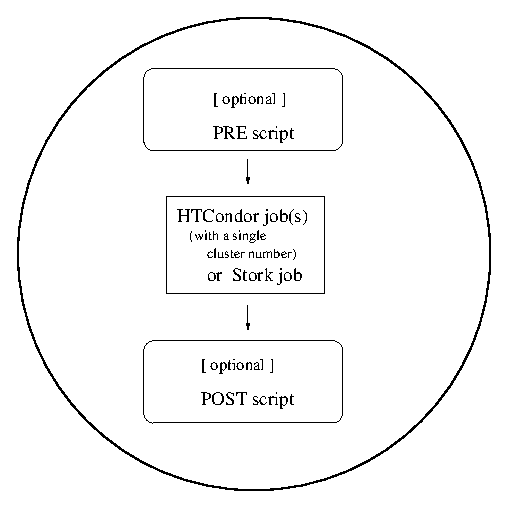
\includegraphics{user-man/dagman-node.eps}
\caption{\label{fig:dagman-node}One Node within a DAG}
\end{figure}

At one time,
the number of HTCondor jobs per node was restricted to one.
This restriction is now relaxed such that all HTCondor jobs
within a node must share a single cluster number.
See the
\Condor{submit} manual page
for a further definition of a cluster.
A limitation exists such that
all jobs within the single cluster must use the same log file.
Separate nodes within a DAG may use different log files.

As DAGMan schedules and submits jobs within nodes to HTCondor,
these jobs are defined to succeed or fail based on their
return values.
This success or failure is propagated in well-defined ways to the level of
a node within a DAG.
Further progression of computation
(towards completing the DAG)
may be defined based upon the success or failure of one or more nodes.

The failure of a single job within a cluster
of multiple jobs
(within a single node)
causes the entire cluster of jobs to fail.
Any other jobs within the failed cluster of jobs are
immediately removed.
Each node within a DAG is further defined to succeed or fail,
based upon the return values of a PRE script, the job(s)
within the cluster, and/or a POST script.

%%%%%%%%%%%%%%%%%%%%%%%%%%%%%%%%%%%%%%%
\subsection{Input File Describing the DAG: the JOB, DATA, SCRIPT and PARENT...CHILD Key Words}
%%%%%%%%%%%%%%%%%%%%%%%%%%%%%%%%%%%%%%%

\index{DAGMan!DAG input file}
The input file used by DAGMan is called a DAG input file.
All items are optional, but there must be at least one \Arg{JOB}
or \Arg{DATA} item.

Comments may be placed in the DAG input file.
The pound character (\verb@#@) as the first character on a
line identifies the line as a comment.
Comments do not span lines.

A simple diamond-shaped DAG, as shown in
Figure~\ref{fig:dagman-diamond}
is presented as a starting point for examples.
This DAG contains 4 nodes.

\begin{figure}[hbt]
\centering
\includegraphics{user-man/dagman-diamond.eps}
\caption{\label{fig:dagman-diamond}Diamond DAG}
\end{figure}


A very simple DAG input file for this diamond-shaped DAG is

\footnotesize
\begin{verbatim}
    # File name: diamond.dag
    #
    JOB  A  A.condor 
    JOB  B  B.condor 
    JOB  C  C.condor	
    JOB  D  D.condor
    PARENT A CHILD B C
    PARENT B C CHILD D
\end{verbatim}
\normalsize

A set of basic key words appearing in a DAG input file is described below.

\begin{itemize}

\label{dagman:JOB}
\index{DAGMan input file!JOB key word}
\item \Bold{JOB}

The \Arg{JOB} key word specifies a job to be managed by HTCondor.
The syntax used for each \Arg{JOB} entry is

\Opt{JOB} \Arg{JobName} \Arg{SubmitDescriptionFileName}
\oOptArg{DIR}{directory} \oOpt{NOOP} \oOpt{DONE}

A \Arg{JOB} entry maps a \Arg{JobName} to an HTCondor submit description file.
The \Arg{JobName} uniquely identifies nodes within the
DAGMan input file and in output messages.
Note that the name for each node within the DAG
must be unique.

The key words \Arg{JOB}, \Arg{DIR}, \Arg{NOOP}, and \Arg{DONE}
are not case sensitive.
Therefore, \Arg{DONE}, \Arg{Done}, and \Arg{done} are all equivalent.
The values defined for \Arg{JobName} and \Arg{SubmitDescriptionFileName}
are case sensitive, as file names in
the Unix file system are case sensitive.
The \Arg{JobName} can be any string that contains no white space, except
for the strings \Arg{PARENT} and \Arg{CHILD} (in upper, lower, or mixed
case).

Note that \Arg{DIR}, \Arg{NOOP}, and \Arg{DONE}, if used, must appear
in the order shown above.

The \Arg{DIR} option specifies a working directory
for this node,
from which the HTCondor job will be submitted,
and from which a \Arg{PRE} and/or
\Arg{POST} script will be run.
Note that a DAG containing \Arg{DIR} specifications cannot
be run in conjunction with the \Arg{-usedagdir} command-line
argument to \Condor{submit\_dag}.  A rescue DAG generated by
a DAG run with the \Arg{-usedagdir} argument will contain
\Arg{DIR} specifications, so the \Arg{-usedagdir} argument is
automatically disregarded when running a rescue DAG.

\label{dagman:NOOP}
The optional \Arg{NOOP} keyword identifies that the HTCondor job within
the node is not to be submitted to HTCondor.
This optimization is useful in cases such as debugging a complex DAG structure,
where some of the individual jobs are long-running.
For this debugging of structure,
some jobs are marked as \Arg{NOOP}s, and
the DAG is initially run to verify that the control flow through
the DAG is correct.
The \Arg{NOOP} keywords are then removed before submitting the DAG.
Any PRE and POST scripts
for jobs specified with \Arg{NOOP} \emph{are} executed;
to avoid running the PRE and POST scripts, comment them out.
The job that is not submitted to HTCondor is given a return value that indicates
success, such that the node may also succeed.
Return values of any 
PRE and POST scripts may still cause the node to fail.
Even though the job specified with \Arg{NOOP} is not submitted,
its submit description file must exist;
the log file for the job is used, 
because DAGMan generates dummy submission and termination events for the job.

The optional \Arg{DONE} keyword identifies a node as being already
completed.
This is mainly used by rescue DAGs generated by DAGMan itself,
in the event of a failure to complete the workflow.
Nodes with the \Arg{DONE} keyword are not executed when the rescue DAG is run,
allowing the workflow to pick up from the previous endpoint.  Users
should generally not use the \Arg{DONE} keyword.
The \Arg{NOOP} keyword is more flexible in avoiding
the execution of a job within a node.
Note that, for any node marked \Arg{DONE} in a DAG, all of
its parents must also be marked \Arg{DONE}; 
otherwise, a fatal error will result.
The \Arg{DONE} keyword applies to the entire node.
A node marked with \Arg{DONE} will not have a PRE or POST script run,
and the HTCondor job will not be submitted.

\label{dagman:DATA}
\index{DAGMan input file!DATA key word}
\item \Bold{DATA}

The \Arg{DATA} key word specifies a job to be managed by the Stork data
placement server.  
Stork software is provided by the Stork project.
Please refer to their website: 
\URL{http://www.cct.lsu.edu/~kosar/stork/index.php}.

The syntax used for each \Arg{DATA} entry is

\Opt{DATA} \Arg{JobName} \Arg{SubmitDescriptionFileName}
\oOptArg{DIR}{directory} \oOpt{NOOP} \oOpt{DONE}

A \Arg{DATA} entry maps a \Arg{JobName} to a Stork submit description file.
In all other respects, the \Arg{DATA} key word is identical to the
\Arg{JOB} key word.

The keywords \Arg{DIR}, \Arg{NOOP} and \Arg{DONE} 
follow the same rules and restrictions, and they have the same effect
for \Opt{DATA} nodes as they do for \Opt{JOB} nodes.

Here is an example of a simple DAG that stages in data using Stork,
processes the data using HTCondor, 
and stages the processed data out using Stork.
Depending upon the implementation, multiple data jobs to stage in data
or to stage out data
may be run in parallel.

\footnotesize
\begin{verbatim}
    DATA    STAGE_IN1  stage_in1.stork
    DATA    STAGE_IN2  stage_in2.stork
    JOB     PROCESS    process.condor 
    DATA    STAGE_OUT1 stage_out1.stork
    DATA    STAGE_OUT2 stage_out2.stork
    PARENT  STAGE_IN1 STAGE_IN2 CHILD PROCESS
    PARENT  PROCESS CHILD STAGE_OUT1 STAGE_OUT2
\end{verbatim}
\normalsize

\label{dagman:SCRIPT}
\index{DAGMan input file!SCRIPT key word}
\item \Bold{SCRIPT}
\index{DAGMan!PRE and POST scripts}

The \Arg{SCRIPT} key word specifies
processing that is done either before a job within
the DAG is submitted to HTCondor or Stork for execution
or after
a job within
the DAG completes its execution.
\index{DAGMan!PRE script}
Processing done before a job is submitted to HTCondor or Stork is
called a \Arg{PRE} script.
Processing done after a job completes
its execution under HTCondor or Stork is
\index{DAGMan!POST script}
called a \Arg{POST} script.
A node in the DAG is comprised of the job together with
\Arg{PRE} and/or \Arg{POST} scripts.

\Arg{PRE} and \Arg{POST} script lines within the DAG input file
use the syntax:

\Opt{SCRIPT} \Opt{PRE} \Arg{JobName} \Arg{ExecutableName} \oArg{arguments}

\Opt{SCRIPT} \Opt{POST}  \Arg{JobName} \Arg{ExecutableName} \oArg{arguments}

The \Arg{SCRIPT} key word identifies the type of line within
the DAG input file.
The \Arg{PRE} or \Arg{POST} key word
specifies the relative timing of when the script is to be run.
The \Arg{JobName} specifies the node to which the script is attached.
The \Arg{ExecutableName}
specifies the script to be executed, and it
may be followed by any command line arguments to that script.
The \Arg{ExecutableName} and optional \Arg{arguments} are
case sensitive; they have their case preserved.  \Bold{Note that neither
the \Arg{ExecutableName} nor the individual arguments within the
\Arg{arguments} string can contain spaces.}

Scripts are optional for each job, and
any scripts are executed on the machine
from which the DAG is submitted; this is not necessarily
the same machine upon which the node's HTCondor or Stork job is run.
Further, a single cluster of HTCondor jobs may be
spread across several machines.

A PRE script is commonly used
to place files in a staging area for the cluster of jobs to use.
A POST script is commonly used
to clean up or remove files once the cluster of jobs is finished running.
An example uses PRE and POST scripts to stage files
that are stored on tape.
The PRE script reads compressed input files from the tape drive,
and it uncompresses them, placing the input files in the current directory.
The cluster of HTCondor jobs reads these input files
and produces output files.
The POST script compresses the output files, writes them out to
the tape, and then removes both the staged input files and the output files.

DAGMan takes note of the exit value of the scripts as well as the job or jobs
within the cluster.  
A script with an exit value not equal to 0 fails.  
If the PRE script fails, 
then the job does not run, but the POST script does run.
The exit value of the POST script determines the success of the job. 
If this behavior is not desired, 
the configuration variable \MacroNI{DAGMAN\_ALWAYS\_RUN\_POST} 
should be set to \Expr{False};
then \Condor{dagman} will not run the POST script if the PRE script fails---%
the node will instead simply fail, 
with neither the job nor the POST script being executed.
If the PRE script succeeds, the HTCondor or Stork job is submitted.
If the job or any one of the jobs within the single cluster fails and there is
no POST script, 
the DAG node is marked as failed.  
An exit value not equal to 0 indicates program failure,
except as indicated by the \Arg{PRE\_SKIP} command:
if a PRE script exits with the PRE\_SKIP value, 
then the node succeeds and the job and the POST script are both skipped.  
It is therefore important that a
successful program return the exit value 0. 
It is good practice to always
explicitly specify a return value in the PRE script,
returning 0 in the case of success.
Otherwise,
the return code of the last completed process is returned,
which can lead to unexpected results. 

If the job fails and there is a POST script,
node failure is determined by the exit value of the POST script.
A failing value from the POST script marks the node as failed.
A succeeding value from the POST script (even with a failed
job) marks the node as successful.
Therefore, the POST script may need to consider the return
value from the job.

By default, the POST script is run regardless of the job's
return value. As for the PRE script, it is recommended to 
specify return values explicitly in the POST script. 
Otherwise the return code of the last completed process 
is returned, which can lead to unexpected results. 

A node not marked as failed at any point is successful.
Table~\ref{Node-success-failure}
summarizes the success or failure of an entire node
for all possibilities.
An \Arg{S} stands for success,
an \Arg{F} stands for failure,
and the dash character (\Arg{-}) identifies that there is no script. The
asterisk (${}^\ast$) indicates that the POST script is run, unless
\MacroNI{DAGMAN\_ALWAYS\_RUN\_POST} is \Expr{False}, in which case the node
will simply fail, as described above.

\begin{center}
\begin{table}[hbt]
\begin{tabular}{|c||cccccccccccccc|} \hline
PRE   & - & - & F          & F          & S & S & - & - & - & - & S & S & S & S  \\
JOB   & S & F & not run    & not run    & S & F & S & S & F & F & S & F & F & S  \\
POST  & - & - & S${}^\ast$ & F${}^\ast$ & - & - & S & F & S & F & S & S & F & F  \\
\hline \hline
node  & S & F & S${}^\ast$ & F          & S & F & S & F & S & F & S & S & F & F  \\
\hline
\end{tabular}
\caption{\label{Node-success-failure}Node success or failure definition }
\end{table}
\end{center}

\index{DAGMan input file!PRE\_SKIP key word}
\index{DAGMan!PRE\_SKIP command}
The behavior of DAGMan with respect to node success or failure can be changed 
with the addition of a \Arg{PRE\_SKIP} command. 
A \Arg{PRE\_SKIP} line within the DAG input file uses the syntax: 

\Opt{PRE\_SKIP} \Arg{JobName} \Arg{non-zero-exit-code}

A DAG input file with this command uses the exit value from the
PRE script of the node specified by \Arg{JobName}. 
If the PRE script terminates with the exit code \Arg{non-zero-exit-code},
then the remainder of the node is skipped entirely.  
Both the job associated with the node and
any \Arg{POST} script will not be executed,
and the node will be marked as successful.

Eight variables (\Env{\$JOB}, \Env{\$JOBID}, \Env{\$RETRY},
\Env{\$MAX\_RETRIES}, \Env{\$RETURN}, \Env{\$PRE\_SCRIPT\_RETURN},
\Env{\$DAG\_STATUS} and \Env{\$FAILED\_COUNT}) can be used within the DAG input
file as arguments passed to a PRE or POST script. 
The use of these variables must be as an individual argument,
and thus will be separated from other arguments by white space character(s).
An example which will \emph{not} cause the substitution of 
the \Env{\$RETURN} value is
\begin{verbatim}
  job_status=$RETURN 
\end{verbatim}
The argument will be this entire string as shown.

\index{DAGMan!JOB@\verb^$JOB^ value}
The variable \Env{\$JOB} evaluates to the (case sensitive) string
defined for \Arg{JobName}.

\index{DAGMan!RETRY@\verb^$RETRY^ value}
The variable \Env{\$RETRY} evaluates to an 
integer value set to 0 the first time a node is run,
and is  incremented each time the node is retried. 
See section~\ref{dagman:retry} for the description of how to cause
nodes to be retried. 

\index{DAGMan!MAX_RETRIES@\verb^$MAX_RETRIES^ value}
The variable \Env{\$MAX\_RETRIES} evaluates to an integer value set 
to the maximum number of retries for the node.
See section~\ref{dagman:retry} for the description of how to cause
nodes to be retried.  
If no retries are set for the node,
\Env{\$MAX\_RETRIES} will be set to 0.

\index{DAGMan!JOBID@\verb^$JOBID^ value}
\index{job ID!defined for a DAGMan node job}
\index{job!job ID!defined for a DAGMan node job}
For use as an argument to POST scripts only, the variable \Env{\$JOBID}
evaluates to a representation of the HTCondor job ID of the node job.
It is the value of the job ClassAd attribute \Attr{ClusterId},
followed by a period,
and then followed by the value of the job ClassAd attribute \Attr{ProcId}.
An example of a job ID might be 1234.0.
For nodes with multiple jobs in the same cluster,
the \Attr{ProcId} value is the one of the last job within the cluster.

\index{DAGMan!Return@\verb^$RETURN^ value}
For use as an argument to POST scripts only,
the \Env{\$RETURN} variable evaluates to the return value of the 
HTCondor or Stork job, if there is a single job within a cluster.
With multiple jobs within the same cluster,
there are two cases to consider.
In the first case, all jobs within the cluster are successful;
the value of \Env{\$RETURN} will be 0, indicating success.
In the second case,
one or more jobs from the cluster fail.
When \Condor{dagman} sees the first terminated event for a job that failed,
it assigns that job's return value as the value
of \Env{\$RETURN}, and attempts to remove all remaining jobs within the cluster.
Therefore, if multiple jobs in the cluster fail with different exit codes,
a race condition determines which exit code gets assigned to \Env{\$RETURN}.

A job that dies due to a signal is reported with a \Env{\$RETURN} value
representing the additive inverse of the signal number.
For example, SIGKILL (signal 9) is reported as -9.
A job whose batch system submission fails is reported as -1001.
A job that is externally removed from the batch system queue
(by something other than \Condor{dagman}) is reported as -1002.

\index{DAGMan!PRE_SCRIPT_RETURN@\verb^$PRE_SCRIPT_RETURN^ value}
For use as an argument to POST scripts only, 
the \Env{\$PRE\_SCRIPT\_RETURN}
variable evaluates to the return value of the PRE script of a node, 
if there is one.
If there is no PRE script, this value will be $-1$.
If the node job was skipped because of failure of the PRE script,
the value of \Env{\$RETURN} will be $-1004$
and the value of \Env{\$PRE\_SCRIPT\_RETURN} will be the exit value
of the PRE script;
the POST script can use this to see if the PRE script exited
with an error condition, and assign success or failure to the node, as
appropriate.

\Env{\$DAG\_STATUS} and \Env{\$FAILED\_COUNT} are documented in
section ~\ref{sec:DAGFinalNode} below.

As an example, consider the diamond-shaped DAG example.
Suppose the PRE script expands a compressed file 
needed as input to nodes B and C.
The file is named of the form
\File{\Arg{JobName}.gz}.
The DAG input file becomes 

\footnotesize
\begin{verbatim}
    # File name: diamond.dag
    #
    JOB  A  A.condor 
    JOB  B  B.condor 
    JOB  C  C.condor	
    JOB  D  D.condor
    SCRIPT PRE  B  pre.csh $JOB .gz
    SCRIPT PRE  C  pre.csh $JOB .gz
    PARENT A CHILD B C
    PARENT B C CHILD D
\end{verbatim}
\normalsize

The script \File{pre.csh} uses the arguments to form the file name
of the compressed file:

\begin{verbatim}
    #!/bin/csh
    gunzip $argv[1]$argv[2]
\end{verbatim}

% $ % this comment just has a dollar sign so that emacs will not think
%	  we're inside of a math section and will draw things more nicely


\label{dagman:ParentChild}
\index{DAGMan input file!PARENT \Dots CHILD key word}
\item \Bold{PARENT \Dots CHILD}

The \Arg{PARENT} and \Arg{CHILD} key words specify the
dependencies within the DAG.
\index{DAGMan!describing dependencies}
Nodes are parents and/or children within the DAG.
A parent node must be completed successfully before
any of its children may be started.
A child node may only be started once
all its parents have successfully completed.

The syntax of a dependency line within the DAG input file:

\Opt{PARENT} \Arg{ParentJobName\Dots} \Opt{CHILD} \Arg{ChildJobName\Dots}

The \Arg{PARENT} key word is followed by one or more
\Arg{ParentJobName}s.
The \Arg{CHILD} key word is followed by one or more
\Arg{ChildJobName}s.
Each child job depends on every parent job within the line.
A single line in the input file can specify the dependencies from one or more
parents to one or more children.
As an example, the line
\begin{verbatim}
PARENT p1 p2 CHILD c1 c2
\end{verbatim}
produces four dependencies:
\begin{enumerate}
\item{\verb@p1@ to \verb@c1@}
\item{\verb@p1@ to \verb@c2@}
\item{\verb@p2@ to \verb@c1@}
\item{\verb@p2@ to \verb@c2@}
\end{enumerate}

\end{itemize}

%%%%%%%%%%%%%%%%%%%%%%%%%%%%%%%%%%%%%%%
\subsection{Submit Description File Contents and Usage of Log Files}
%%%%%%%%%%%%%%%%%%%%%%%%%%%%%%%%%%%%%%%

\index{DAGMan!submit description file with}
\index{DAGMan!usage of log files}
Each node in a DAG may use a unique submit description file.
One key limitation is that
each HTCondor submit description file must submit jobs
described by a single cluster number.
At the present time DAGMan cannot deal with a submit file producing
multiple job clusters.

\emph{DAGMan enforces the dependencies within a DAG
using the events recorded in the
log file(s) produced by job submission to HTCondor.}
At one time, DAGMan required that all jobs within all nodes
specify the same, single log file.
This is no longer the case.
However, if the DAG utilizes a large number of
separate log files, performance may suffer.
Therefore, it is better to have
fewer, or even only a single log file.
%Unfortunately,
%each Stork job currently requires a separate log file.

\index{DAGMan!lazy log file evaluation}
As of HTCondor version 7.3.2, DAGMan's handling of log files
significantly changed to improve resource usage and efficiency.  
Prior to HTCondor version 7.3.2, 
DAGMan assembled a list of all relevant log files at start up, 
by looking at all of the submit description files for all of the nodes.
It kept the log files open for the duration of the DAG.
Beginning with HTCondor version 7.3.2, DAGMan delays opening and using 
the submit description file until just before it is going to submit the job.
At that point, DAGMan reads the submit description file to discover 
the job's log file.
And, DAGMan monitors only the log files that are relevant
to the jobs currently queued, 
or associated with nodes for which a POST script is running.

The advantages of the new "lazy log file evaluation" scheme are:

\begin{itemize}

\item The \Condor{dagman} executable uses fewer file descriptors.
In specific,
DAGMan must keep a file descriptor open for each unique log file,
and operating systems limit the number of open file descriptors;
HTCondor's most severe limit is 2048 on Windows platforms.

\item It is much easier to have one node of a DAG produce the
submit description file for a descendant node in the DAG.

\end{itemize}

There is one known disadvantage of the lazy log file evaluation scheme:

\begin{itemize}

\item Because the log files are internally identified by inode
numbers, it is possible that errors may arise where log files for
a given DAG are spread across more than one device.
This permits two unique files to have the same inode number.
We hope to have this problem fixed soon.

\end{itemize}

\index{DAGMan!default log file specification}
%Another new feature in HTCondor version 7.3.2 was the use of 
DAGMan assigns 
default node job user logs,
if a log file is not specified within a job's submit description file.
In HTCondor versions earlier than 7.3.2, 
it was a fatal error if the submit description
file for a node job did not specify a log file.
The file used as the default node log is controlled by the
\MacroNI{DAGMAN\_DEFAULT\_NODE\_LOG} configuration variable.
A complete description is at section~\ref{param:DAGManDefaultNodeLog}.
Nodes specifying a log file and other nodes using the default log
file can be mixed in a single DAG.
Allowing DAGMan to specify a single log file for an entire DAG, 
especially a wide DAG,
reduces the number of concurrently open file descriptors.

Log files for node jobs should not be placed on NFS, 
unless both configuration variables
\Macro{CREATE\_LOCKS\_ON\_LOCAL\_DISK} and \Macro{ENABLE\_USERLOG\_LOCKING}
are \Expr{True}. 
Without these settings, NFS file locking is not reliable,
occasionally resulting in simultaneous acquisition of locks on a single
log file by both the \Condor{schedd} daemon and the \Condor{dagman} job. 
Partially written events by the \Condor{schedd} cause errors
for \Condor{dagman}.

An additional restriction applies to the submit description file
command \SubmitCmd{Log} specific to an HTCondor job within
a DAG node.
\emph{This command may not be defined in such a way that it uses macros.}
Using a macro would violate the restriction that there be exactly
one log file specified for the potentially multiple jobs 
within a single cluster.

Here is a modified version of the DAG input file
for the diamond-shaped DAG. 
The modification has each node use the same 
submit description file.

\begin{verbatim}
    # File name: diamond.dag
    #
    JOB  A  diamond_job.condor 
    JOB  B  diamond_job.condor 
    JOB  C  diamond_job.condor	
    JOB  D  diamond_job.condor
    PARENT A CHILD B C
    PARENT B C CHILD D
\end{verbatim}

Here is the single HTCondor submit description file
for this DAG:

\index{DAGMan!example submit description file}
\begin{verbatim}
    # File name: diamond_job.condor
    #
    executable   = /path/diamond.exe
    output       = diamond.out.$(cluster)
    error        = diamond.err.$(cluster)
    log          = diamond_condor.log
    universe     = vanilla
    notification = NEVER
    queue
\end{verbatim}

This example uses the same HTCondor submit description file
for all the jobs in the DAG.
This implies that each node within the DAG runs the
same job.
The \MacroUNI{cluster} macro
produces unique file names for each job's output.
As the HTCondor job within each node
causes a separate job submission, each has a unique cluster number.

Notification is set to \verb@NEVER@ in this example.
This tells HTCondor not to send e-mail about the completion of a job
submitted to HTCondor.
For DAGs with many nodes, this
reduces or eliminates excessive numbers of e-mails.

\index{ClassAd job attribute!DAGParentNodeNames}
\index{DAGParentNodeNames!job ClassAd attribute}
The job ClassAd attribute \Attr{DAGParentNodeNames} is also available
for use within the submit description file. 
It defines a comma separated list of each \Arg{JobName}
which is a parent node of this job's node.
This attribute may be used in the \SubmitCmd{arguments} command
for all but scheduler universe jobs.
For example, if the job has two parents, with \Arg{JobName}s B and C,
the submit description file command
\begin{verbatim}
arguments = $$([DAGParentNodeNames])
\end{verbatim}
will pass the string \AdStr{B,C} as the command line argument when invoking
the job.

%%%%%%%%%%%%%%%%%%%%%%%%%%%%%%%%%%%%%%%
\subsection{\label{dagman:submitdag}DAG Submission}
%%%%%%%%%%%%%%%%%%%%%%%%%%%%%%%%%%%%%%%

A DAG is submitted using the program \Condor{submit\_dag}.
See the manual
page~\pageref{man-condor-submit-dag}
for complete details.
A simple submission has the syntax

\Condor{submit\_dag} \Arg{DAGInputFileName}

\index{DAGMan!job submission}
The diamond-shaped DAG example may be submitted with

\begin{verbatim}
condor_submit_dag diamond.dag
\end{verbatim}
In order to guarantee recoverability, the DAGMan program itself
is run as an HTCondor job.
As such, it needs a submit description file.
\Condor{submit\_dag} produces this needed submit description file,
naming it by appending \File{.condor.sub} to the \Arg{DAGInputFileName}.
This submit description file may be edited if the DAG is
submitted with

\begin{verbatim}
condor_submit_dag -no_submit diamond.dag
\end{verbatim}
causing \Condor{submit\_dag} to generate the submit description file,
but not submit DAGMan to HTCondor.
To submit the DAG, once the submit description file is edited,
use

\begin{verbatim}
condor_submit diamond.dag.condor.sub
\end{verbatim}

An optional argument to \Condor{submit\_dag}, \Arg{-maxjobs}, 
is used to specify the maximum number of batch jobs that DAGMan may
submit at one time.
It is commonly used when 
there is a limited amount of input file staging capacity.
As a specific example, consider a case where each job will
require 4 Mbytes of input files,
and the jobs will run in a directory with a volume of 100 Mbytes
of free space.
Using the argument \Arg{-maxjobs 25} guarantees that a maximum
of 25 jobs, using a maximum of 100 Mbytes of space,
will be submitted to HTCondor and/or Stork at one time.

% -maxscripts has been replaced with -maxpre and -maxpost
% Similarly, the \Arg{maxscripts} argument is used to specify the
% maximum number of PRE and POST scripts running at one time.
While the \Arg{-maxjobs} argument is used to limit the number
of batch system jobs submitted at one time,
it may be desirable to limit the number of scripts running
at one time.
The optional \Arg{-maxpre} argument limits the number of PRE
scripts that may be running at one time,
while the optional \Arg{-maxpost} argument limits the number of POST
scripts that may be running at one time.

An optional argument to \Condor{submit\_dag}, \Arg{-maxidle}, 
is used to limit the number of idle jobs within a given DAG.
When the number of idle node jobs in the DAG reaches the specified
value, \Condor{dagman} will stop submitting jobs, even if there
are ready nodes in the DAG.  Once some of the idle jobs start to
run, \Condor{dagman} will resume submitting jobs.  Note that this
parameter only limits the number of idle jobs submitted by a
given instance of \Condor{dagman}. Idle jobs submitted by other sources
(including other \Condor{dagman} runs) are ignored. 
Also, \Condor{dagman}
does not do anything special to the submit description file.
If a submit description file contains
\Expr{queue 5000} and there is a specification for the \Arg{-maxidle} 
argument of 250, 
\Condor{dagman} will submit the file, 
and a new cluster of 5000 jobs will be submitted to the \Condor{schedd}.
In this case, no further jobs will be submitted by \Condor{dagman}
until the number of idle jobs falls below 250. 

%%%%%%%%%%%%%%%%%%%%%%%%%%%%%%%%%%%%%%%
\subsection{Job Monitoring, Job Failure, and Job Removal}
%%%%%%%%%%%%%%%%%%%%%%%%%%%%%%%%%%%%%%%

After submission, the progress of the DAG can be monitored
by looking at the log file(s),
observing the e-mail that job submission to HTCondor causes,
or by using \Condor{q} \Arg{-dag}.
There is a large amount of information in an extra file.
The name of this extra file is produced by appending
\File{.dagman.out} to \Arg{DAGInputFileName}; for example, if the
DAG file is \File{diamond.dag}, this extra file is
\File {diamond.dag.dagman.out}.
If this extra file grows too large, limit its size
with the \Macro{MAX\_DAGMAN\_LOG} configuration macro (see
section~\ref{param:MaxSubsysLog}).

If you have some kind of problem in your DAGMan run, please save
the corresponding \File{dagman.out} file; it is the most important
debugging tool for DAGMan.  As of version 6.8.2, the \File{dagman.out}
is appended to, rather than overwritten, with each new DAGMan run.


\Condor{submit\_dag} attempts to check the DAG input file.
If a problem is detected,
\Condor{submit\_dag} prints out an error message and aborts.

To remove an entire DAG, consisting of DAGMan plus
any jobs submitted to HTCondor or Stork,
remove the DAGMan job running under HTCondor.
\Condor{q} will list the job number.
Use the job number to remove the job, for example

\footnotesize
\begin{verbatim}

% condor_q
-- Submitter: turunmaa.cs.wisc.edu : <128.105.175.125:36165> : turunmaa.cs.wisc.edu
 ID      OWNER          SUBMITTED     RUN_TIME ST PRI SIZE CMD
  9.0   smoler         10/12 11:47   0+00:01:32 R  0   8.7  condor_dagman -f -
 11.0   smoler         10/12 11:48   0+00:00:00 I  0   3.6  B.out
 12.0   smoler         10/12 11:48   0+00:00:00 I  0   3.6  C.out

    3 jobs; 2 idle, 1 running, 0 held

% condor_rm 9.0
\end{verbatim}
\normalsize

Before the DAGMan job stops running, it uses \Condor{rm}
%Before the DAGMan job stops running, it uses \Condor{rm} and/or
%\Stork{rm} 
to remove any jobs within the DAG that are running.

In the case where a
machine is scheduled to go down,
DAGMan will clean up memory and exit.
However, it will leave any submitted jobs
in HTCondor's queue.

%%%%%%%%%%%%%%%%%%%%%%%%%%%%%%%%%%%%%%%
\subsection{\label{sec:DagSuspend}Suspending a Running DAG}
%%%%%%%%%%%%%%%%%%%%%%%%%%%%%%%%%%%%%%%

It may be desired to temporarily suspend a running DAG.
For example, the load may be high on the submit machine,
and therefore it is desired to prevent DAGMan from
submitting any more jobs until the load goes down.
There are two ways to suspend (and resume) a running DAG.

\begin{itemize}
\item Use \Condor{hold}/\Condor{release} on the \Condor{dagman} job.

After placing the \Condor{dagman} job on hold,
no new node jobs will be submitted,
and no PRE or POST scripts will be run.
Any node jobs already in the HTCondor queue will continue undisturbed.
If the \Condor{dagman} job is left on hold,
it will remain in the HTCondor queue after all of the currently running
node jobs are finished.
To resume the DAG, use \Condor{release} on the \Condor{dagman} job.

Note that while the \Condor{dagman} job is on hold,
no updates will be made to the \File{dagman.out} file.

\item Use a DAG halt file.

The second way of suspending a DAG uses the existence of a specially-named
file to change the state of the DAG.
When in this halted state,
no PRE scripts will be run, and no node jobs will be submitted.  
Running node jobs will continue undisturbed.
A halted DAG will still run POST scripts,
and it will still update the \File{dagman.out} file.
This differs from behavior of a DAG that is held.
Furthermore, a halted DAG will not remain in the queue indefinitely;
when all of the running node jobs have finished, 
DAGMan will create a Rescue DAG and exit.

To resume a halted DAG, remove the halt file.

The specially-named file must be placed in the same directory
as the DAG input file.
The naming is the same as the DAG input file concatenated with the
string \File{.halt}.
For example, if the DAG input file is \File{test1.dag}, 
then \File{test1.dag.halt} will be the required name of the halt file.

As any DAG is first submitted with \Condor{submit\_dag}, 
a check is made for a halt file.
If one exists, it is removed.
\end{itemize}

%%%%%%%%%%%%%%%%%%%%%%%%%%%%%%%%%%%%%%%
\subsection{\label{sec:AdvDAGMan}Advanced Features of DAGMan}
%%%%%%%%%%%%%%%%%%%%%%%%%%%%%%%%%%%%%%%


%%%%%%%%%%%%%%%%%%%%%%%%%%%%%%%%%%%%%%%
\subsubsection{\label{dagman:retry}Retrying Failed Nodes or Stopping the Entire DAG}

\index{DAGMan input file!RETRY key word}
\index{DAGMan!RETRY of failed nodes}
\index{DAGMan input file!ABORT-DAG-ON key word}
\index{DAGMan!ABORT-DAG-ON}

The \Arg{RETRY} key word provides a
way to retry failed nodes.
The use of retry is optional.
The syntax for retry is

\Opt{RETRY} \Arg{JobName} \Arg{NumberOfRetries} \oOptArg{UNLESS-EXIT}{value}

where \Arg{JobName} identifies the node.
\Arg{NumberOfRetries} is an integer
number of times to retry the node after failure.
The implied number of retries for any node is 0,
the same as not having a retry line in the file. 
Retry is implemented on nodes, not parts of a node.

The diamond-shaped DAG example may be modified to
retry node C:

\footnotesize
\begin{verbatim}
    # File name: diamond.dag
    #
    JOB  A  A.condor 
    JOB  B  B.condor 
    JOB  C  C.condor	
    JOB  D  D.condor
    PARENT A CHILD B C
    PARENT B C CHILD D
    Retry  C 3
\end{verbatim}
\normalsize

If node C is marked as failed (for any reason),
then it is started over as a first retry.
The node will be tried a second and third time,
if it continues to fail.
If the node is marked as successful, then further retries do not occur.

Retry of a node may be short circuited using the
optional key word \Arg{UNLESS-EXIT} (followed by an
integer exit value).
If the node exits with the specified integer exit value,
then no further processing will be done
on the node. 

The variable \Env{\$RETRY} evaluates to an 
integer value set to 0 first time a node is run,
and is  incremented each time for each time the node is retried. 
The variable \Env{\$MAX\_RETRIES} is the value set for
\Arg{NumberOfRetries}.


The \Arg{ABORT-DAG-ON} key word provides a way
to abort the entire DAG if a given node returns a specific exit
code.  The syntax for \Arg{ABORT-DAG-ON} is

\Opt{ABORT-DAG-ON} \Arg{JobName} \Arg{AbortExitValue}
\oOptArg{RETURN}{DAGReturnValue}

If the node specified by \Arg{JobName} returns the specified
\Arg{AbortExitValue}, the
DAG is immediately aborted.
A DAG abort differs from a node failure,
in that a DAG abort causes all nodes within the DAG to be stopped immediately.
This includes removing the jobs in nodes that are currently running.
A node failure allows the DAG to continue running,
until no more progress can be made due to dependencies.

An abort overrides node retries. 
If a node returns the abort exit value,
the DAG is aborted,
even if the node has retry specified.

When a DAG aborts, by default it exits with the node return value that
caused the abort.  This can be changed by 
using  the optional \Arg{RETURN} key word along
with specifying the desired \Arg{DAGReturnValue}.
The DAG abort return value
can be used for DAGs within DAGs,
allowing an inner DAG to cause an abort of an outer DAG.

Adding \Arg{ABORT-DAG-ON} for node C in the diamond-shaped
DAG
\footnotesize
\begin{verbatim}
    # File name: diamond.dag
    #
    JOB  A  A.condor 
    JOB  B  B.condor 
    JOB  C  C.condor	
    JOB  D  D.condor
    PARENT A CHILD B C
    PARENT B C CHILD D
    Retry  C 3
    ABORT-DAG-ON C 10 RETURN 1
\end{verbatim}
\normalsize

causes the DAG to be aborted, if node C exits with a return value of 10.
Any other currently running nodes (only node B is a possibility for 
this particular example) are stopped and removed.
If this abort occurs, the return value for the DAG is 1.


%%%%%%%%%%%%%%%%%%%%%%%%%%%%%%%%%%%%%%%
\subsubsection{\label{dagman:VARS}Variable Values Associated with Nodes}
\index{DAGMan input file!VARS key word}

\index{DAGMan!VARS (macro for submit description file)}
\index{VARS}
The \Arg{VARS} key word provides a
method for defining a macro that can be referenced in the
node's submit description file.
These macros are defined on a per-node basis, using the
following syntax:

\Opt{VARS} \Arg{JobName} \Arg{macroname=}\Arg{"string"} [\Arg{macroname=}\Arg{"string"\Dots]}

The macro may be used within the
submit description file of the relevant node.  A \Arg{macroname}
consists of alphanumeric characters (a..Z and 0..9),
as well as the underscore character.
The space character delimits macros,
when there is more than one macro defined for a node on a single line.
Multiple lines defining macros for the same node are permitted.

Correct syntax requires that the \Arg{string} must be
enclosed in double quotes.
To use a double quote inside \Arg{string},
escape it with the backslash character (\verb@\@).
To add the backslash character itself, use two backslashes (\verb@\\@).
The string \$(JOB) maybe used in \Arg{string} and will expand to
\Arg{JobName}. 
If the \Arg{VARS} line appears in a DAG file used as a splice file, 
then \$(JOB) will be the fully scoped name of the node.

\Bold{Note that the \Arg{macroname} itself cannot begin with the string
\Expr{queue},
in any combination of upper or lower case.}

If the DAG input file contains
\footnotesize
\begin{verbatim}
    # File name: diamond.dag
    #
    JOB  A  A.condor 
    JOB  B  B.condor 
    JOB  C  C.condor	
    JOB  D  D.condor
    VARS A state="Wisconsin"
    PARENT A CHILD B C
    PARENT B C CHILD D

\end{verbatim}
\normalsize

then file \File{A.condor} may use the macro \verb@state@.
This example submit description file for the HTCondor
job in node A passes the value
of the macro as a command-line argument to the job.

\footnotesize
\begin{verbatim}
    # file name: A.condor
    executable = A.exe
    log        = A.log
    error      = A.err
    arguments  = "$(state)"
    queue
\end{verbatim}
\normalsize

This HTCondor job's command line will be
\footnotesize
\begin{verbatim}
A.exe Wisconsin
\end{verbatim}
\normalsize
The use of macros may allow a reduction in the necessary number 
of unique submit description files.

A separate example shows an intended use of a \Arg{VARS} entry
in the DAG input file.
This use may dramatically reduce the number of HTCondor submit description
files needed for a DAG.
In the case where the submit description file for each node
varies only in file naming, the use of a substitution macro
within the submit description file reduces the need to
a single submit description file.
Note that the user log file for a job currently cannot be specified
using a macro passed from the DAG.

The example uses a single submit description file in the DAG input
file, and uses the \Arg{VARS} entry to name output files.

The relevant portion of the DAG input file appears as 
\begin{verbatim}
    JOB A theonefile.sub
    JOB B theonefile.sub
    JOB C theonefile.sub

    VARS A outfilename="A"
    VARS B outfilename="B"
    VARS C outfilename="C"
\end{verbatim}

The submit description file appears as 
\footnotesize
\begin{verbatim}
    # submit description file called:  theonefile.sub
    executable   = progX
    universe     = standard
    output       = $(outfilename)
    error        = error.$(outfilename)
    log          = progX.log
    queue
\end{verbatim}
\normalsize

For a DAG such as this one, but with thousands of nodes,
being able to write and maintain a single submit description file 
and a single, yet more complex, DAG input file is preferable.

% Note: this is an alternative to subsubsubsection, which we don't have.
\begin{description}
\item[Multiple macroname definitions]
\end{description}

If a VARS macroname for a specific node in a DAG input file is defined
more than once,
as it would be with the partial file contents
\begin{verbatim}
  JOB job1 job.condor
  VARS job1 a="foo"
  VARS job1 a="bar"
\end{verbatim}
a warning is written to the log, of the format 
\begin{verbatim}
Warning: VAR <macroname> is already defined in job <JobName>
Discovered at file "<DAG input file name>", line <line number>
\end{verbatim}

The behavior of DAGMan is such that all definitions for the macroname
exist,
but only the last one defined is used as the variable's value.
For example, if the example is within the DAG input file,
and the job's submit description file utilized the value with
\begin{verbatim}
  arguments = "$(a)"
\end{verbatim}
then the argument will be \Expr{bar}.

% Note: this is an alternative to subsubsubsection, which we don't have.
\begin{description}
\item[Special characters within VARS string definitions]
\end{description}

The value of a \Arg{VARS} \Arg{macroname} may contain spaces and tabs.
It is also possible to have double quote marks and
backslashes within these values.
\Bold{Unfortunately, it is not
possible to have single quote marks within these values.}
In order to have spaces or tabs within a value,
use the new syntax format for the \SubmitCmd{arguments} command
in the node's HTCondor job submit description file,
as described in section~\ref{man-condor-submit-arguments}.
Double quote marks are escaped differently,
depending on the new syntax or old syntax argument format.
Note that in both syntaxes,
double quote marks require two levels of escaping:
one level is for the parsing of the DAG input file, and the other level is for
passing the resulting value through \Condor{submit}.

As an example, here are only the relevant parts of a DAG input file.
Note that the NodeA value for \Expr{second} contains a tab.
\footnotesize
\begin{verbatim}
    Vars NodeA first="Alberto Contador"
    Vars NodeA second="\"\"Andy	Schleck\"\""
    Vars NodeA third="Lance\\ Armstrong"
    Vars NodeA misc="!@#$%^&*()_-=+=[]{}?/"
    
    Vars NodeB first="Lance_Armstrong"
    Vars NodeB second="\\\"Andreas_Kloden\\\""
    Vars NodeB third="Ivan\\_Basso"
    Vars NodeB misc="!@#$%^&*()_-=+=[]{}?/"
\end{verbatim}
\normalsize

The new syntax \SubmitCmd{arguments} line of the HTCondor submit description file
for NodeA is
\footnotesize
\begin{verbatim}
  arguments = "'$(first)' '$(second)' '$(third)' '$(misc)'"
\end{verbatim}
\normalsize
The single quotes around each variable reference are only necessary
if the variable value may contain spaces or tabs.
The resulting values passed to the NodeA executable are
\footnotesize
\begin{verbatim}
  Alberto Contador
  "Andy	Schleck"
  Lance\ Armstrong
  !@#$%^&*()_-=+=[]{}?/
\end{verbatim}
\normalsize

The old syntax \SubmitCmd{arguments} line of the HTCondor submit description file
for NodeB is
\footnotesize
\begin{verbatim}
  arguments = $(first) $(second) $(third) $(misc)
\end{verbatim}
\normalsize

The resulting values passed to the NodeB executable are
\footnotesize
\begin{verbatim}
  Lance_Armstrong
  "Andreas_Kloden"
  Ivan\_Basso
  !@#$%^&*()_-=+=[]{}?/
\end{verbatim}
\normalsize

%%%%%%%%%%%%%%%%%%%%%%%%%%%%%%%%%%%%%%%
\subsubsection{Setting Priorities for Nodes}
\index{DAGMan input file!PRIORITY key word}

The \Arg{PRIORITY} key word assigns a priority to a DAG node.
The syntax for \Arg{PRIORITY} is

\Opt{PRIORITY} \Arg{JobName} \Arg{PriorityValue}

The node priority affects the order in which nodes that are ready
at the same time will be submitted.  Note that node priority does
\emph{not} override the DAG dependencies.

Node priority is mainly relevant if
node submission is throttled via the \Arg{-maxjobs} or \Arg{-maxidle}
command-line arguments or the \MacroNI{DAGMAN\_MAX\_JOBS\_SUBMITTED} or
\MacroNI{DAGMAN\_MAX\_JOBS\_IDLE} configuration variables.  Note that PRE
scripts can affect the order in which jobs run, so DAGs containing
PRE scripts may not run the nodes in exact priority order, even if
doing so would satisfy the DAG dependencies.

The priority value is an integer (which can be negative).  A larger
numerical priority is better (will be run before a smaller numerical
value).  The default priority is 0.

Adding \Arg{PRIORITY} for node C in the diamond-shaped
DAG
\footnotesize
\begin{verbatim}
    # File name: diamond.dag
    #
    JOB  A  A.condor 
    JOB  B  B.condor 
    JOB  C  C.condor	
    JOB  D  D.condor
    PARENT A CHILD B C
    PARENT B C CHILD D
    Retry  C 3
    PRIORITY C 1
\end{verbatim}
\normalsize

This will cause node C to be submitted before node B.
Without this priority setting for node C, node B would be submitted first.

Priorities are propagated to children, to SUBDAGs, 
and to the HTCondor job itself,
via the \Attr{JobPrio} attribute in the job's ClassAd. 
The priority is defined to be the maximum of the DAG PRIORITY directive 
for the job itself and the PRIORITYs of all its parents. 
Here is an example to clarify:

\footnotesize
\begin{verbatim}
    # File name: priorities.dag
    #
JOB A A.condor
JOB B B.condor
JOB C C.condor
SUBDAG EXTERNAL D SD.subdag
PARENT A C CHILD B
PARENT C CHILD D
PRIORITY A 60
PRIORITY B 0
PRIORITY C 5
PRIORITY D 100
\end{verbatim}
\normalsize

In this example, node B is a child of nodes A and C. 
Node B's priority is initially set to 0,
but its priority becomes 60,
because that is the maximum of its initial priority of 0,
and the priorities of its parents
A with priority 60 and C with priority 5.
Node D has only parent node C.
Since the priority of node D will become at least as big as that of 
its parent node C,
node D is assigned a priority of 100.
And, all nodes in the D SUBDAG will have priority at least 100.
This priority is assigned by DAGMan.
There is no way to change the priority in the submit description file for a job,
as DAGMan will override any \SubmitCmd{priority} command placed
in a submit description file.
The implication of this priority propagation is
that for DAGs with a large number of edges (representing dependencies), 
the priorities of child nodes far from the root nodes 
will tend to be the same.
The priorities of the leaf nodes of a tree-shaped DAG,
or of DAGs with a relatively small number of dependencies,
will \emph{not} tend to be the same.

%%%%%%%%%%%%%%%%%%%%%%%%%%%%%%%%%%%%%%%
\subsubsection{\label{sec:DAG-node-category}Limiting the Number of Submitted Job Clusters within a DAG}

\index{DAGMan input file!CATEGORY key word}
\index{DAGMan input file!MAXJOBS key word}

In order to limit the number of submitted job clusters within a DAG,
the nodes may be placed into categories by assignment of a name.
Then, a maximum number of submitted clusters may be specified
for each category.

The \Arg{CATEGORY} key word assigns a category name to a DAG node.
The syntax for \Arg{CATEGORY} is

\Opt{CATEGORY} \Arg{JobName} \Arg{CategoryName}

Category names cannot contain white space.

The \Arg{MAXJOBS} key word limits the number of submitted job clusters
on a per category basis.
The syntax for \Arg{MAXJOBS} is

\Opt{MAXJOBS} \Arg{CategoryName} \Arg{MaxJobsValue}

If the number of submitted job clusters for a given category reaches the limit,
no further job clusters in that category will be submitted until other
job clusters within the category terminate.
If MAXJOBS is not set for a defined category,
then there is no limit placed on the number of submissions
within that category.

Note that a single invocation
of \Condor{submit} results in one job cluster.
The number of HTCondor jobs within a cluster may be greater than 1. 

The  configuration variable \MacroNI{DAGMAN\_MAX\_JOBS\_SUBMITTED} 
and the \Condor{submit\_dag} \Arg{-maxjobs} command-line option
are still enforced if these \Arg{CATEGORY} and \Arg{MAXJOBS} throttles are used.

Please see the end of section~\ref{sec:DAGSplicing}
on DAG Splicing for a description of the interaction between
categories and splices.

%%%%%%%%%%%%%%%%%%%%%%%%%%%%%%%%%%%%%%%
\subsubsection{\label{sec:DAG-configuration}Configuration Specific to a DAG}
\index{DAGMan input file!CONFIG key word}
\index{DAGMan!CONFIG}

The \Arg{CONFIG} keyword specifies a configuration file to be used
to set configuration variables related to \Condor{dagman}
when running this DAG.
The syntax for \Arg{CONFIG} is

\Opt{CONFIG} \Arg{ConfigFileName}

If the DAG file contains a line like this,
\begin{verbatim}
    CONFIG dagman.config
\end{verbatim}
then the configuration values in the file \File{dagman.config} will be used
for this DAG.

Configuration macros for \Condor{dagman} can be specified in several
ways, as given within the ordered list:
\begin{enumerate}
\item
In an HTCondor configuration file.
\item
With an environment variable.
Prepend the string \verb@_CONDOR_@ to the configuration variable's name.
\item
As specified above, with a line in the DAG input file
using the keyword \Arg{CONFIG}, such that there is a \Condor{dagman}-specific
configuration file specified,
or on the \Condor{submit\_dag} command line.
\item
For some configuration variables,
there is a corresponding \Condor{submit\_dag} command line argument.
For example, the configuration variable \MacroNI{DAGMAN\_MAX\_JOBS\_SUBMITTED}
has the corresponding command line argument \Arg{-maxjobs}.
\end{enumerate}

In the above list, configuration values specified later in the list
override ones specified earlier
For example, a value specified on the
\Condor{submit\_dag} command line overrides corresponding values in any
configuration file.
And, a value specified in a DAGMan-specific configuration
file overrides values specified in a general HTCondor configuration file.

Configuration variables that are not for \Condor{dagman}
and not utilized by DaemonCore, yet are specified in a
\Condor{dagman}-specific configuration file are ignored.

Only a single configuration file can be specified for a given
\Condor{dagman} run.  For example, if one file is specified within a DAG
input file,
and a different file is specified on the \Condor{submit\_dag} command
line, this is a fatal error at submit time.
The same is true if
different configuration files are specified in multiple DAG input files,
and referenced in a single \Condor{submit\_dag} command.

If multiple DAGs are run in a single \Condor{dagman} run, the
configuration options specified in the \Condor{dagman} configuration
file, if any, apply to all DAGs, even if some of the DAGs specify no
configuration file.

Configuration variables relating to DAGMan may be found
in section~\ref{sec:DAGMan-Config-File-Entries}.

%%%%%%%%%%%%%%%%%%%%%%%%%%%%%%%%%%%%%%%
\subsubsection{\label{sec:MultipleDAGs}Optimization of Submission Time}
%%%%%%%%%%%%%%%%%%%%%%%%%%%%%%%%%%%%%%%

\Condor{dagman} works by watching log files for events, such as submission,
termination, and going on hold.
When a new job is ready to be run, it is submitted to the \Condor{schedd}, 
which needs to acquire a computing resource. 
Acquisition requires the \Condor{schedd} to contact the central
manager and get a claim on a machine,
and this claim cycle can take many minutes.

Configuration variable
\Macro{DAGMAN\_HOLD\_CLAIM\_TIME} 
avoids the wait for a negotiation cycle.
When set to a non zero value, 
the \Condor{schedd} keeps a claim idle,
such that the \Condor{startd} delays in shifting from
the Claimed to the Preempting state (see Figure~\ref{fig:machine-states}).
Thus, if another job appears that is suitable for the claimed resource,
then the \Condor{schedd} will submit the job directly to the \Condor{startd}, 
avoiding the wait and overhead of a negotiation cycle.
This results in a speed up of job completion,
especially for linear DAGs in pools that have lengthy negotiation cycle times.

By default, \MacroNI{DAGMAN\_HOLD\_CLAIM\_TIME} is 20, 
causing a claim to remain idle for 20 seconds, 
during which time a new job can be submitted
directly to the already-claimed \Condor{startd}. 
A value of 0 means that claims are not held idle for a running DAG.
If a DAG node has no children,
the value of \MacroNI{DAGMAN\_HOLD\_CLAIM\_TIME} will be ignored;
the \Attr{KeepClaimIdle} attribute will not be defined in the job ClassAd 
of the node job, unless the job requests it using the submit command
\SubmitCmd{keep\_claim\_idle}. 

%%%%%%%%%%%%%%%%%%%%%%%%%%%%%%%%%%%%%%%
\subsubsection{\label{sec:MultipleDAGs}Single Submission of Multiple, Independent DAGs}
%%%%%%%%%%%%%%%%%%%%%%%%%%%%%%%%%%%%%%%
\index{DAGMan!Single submission of multiple, independent DAGs}

A single use of \Condor{submit\_dag} may execute multiple, independent DAGs.
Each independent DAG has its own DAG input file.
These DAG input files are command-line arguments to
\Condor{submit\_dag}
(see the \Condor{submit\_dag} manual page at ~\ref{man-condor-submit-dag}).

Internally, all of the independent DAGs are combined
into a single, larger DAG, with no dependencies between
the original independent DAGs.
As a result,
any generated rescue DAG file represents all of the input DAGs
as a single DAG.
The file name of this rescue DAG is based on the DAG input file
listed first within the command-line arguments to
\Condor{submit\_dag} (unlike a single-DAG rescue DAG file, however,
the file name will be
\File{\textless{whatever}\textgreater.dag\_multi.rescue} or
\File{\textless{whatever}\textgreater.dag\_multi.rescueNNN},
as opposed to
just \File{\textless{whatever}\textgreater.dag.rescue}
or \File{\textless{whatever}\textgreater.dag.rescueNNN}).
Other files such
as \File{dagman.out} and the lock file also have names based on this
first DAG input file.

The success or failure of the independent DAGs is well defined.
When multiple, independent DAGs are submitted with a single
command, the
success of the composite DAG is defined as the logical AND
of the success of each independent DAG.
This implies that failure is defined as the logical OR
of the failure of any of the independent DAGs.

By default, DAGMan internally renames the nodes to avoid node name collisions.  
If all node names are unique, 
the renaming of nodes may be disabled by
setting the configuration variable \Macro{DAGMAN\_MUNGE\_NODE\_NAMES}
to \Expr{False} (see ~\ref{param:DAGManMungeNodeNames}).


%%%%%%%%%%%%%%%%%%%%%%%%%%%%%%%%%%%%%%%
\subsubsection{\label{sec:DAGsinDAGs}A DAG Within a DAG Is a SUBDAG}
%%%%%%%%%%%%%%%%%%%%%%%%%%%%%%%%%%%%%%%
\index{DAGMan!DAGs within DAGs}
\index{DAGMan input file!SUBDAG key word}

The organization and dependencies of the jobs within a DAG
are the keys to its utility.
Some DAGs are naturally constructed hierarchically,
such that a node within a DAG is also a DAG.
HTCondor DAGMan handles this situation easily.
DAGs can be nested to any depth.

One of the highlights of using the SUBDAG feature is that portions of a DAG
may be constructed and modified during the execution of the DAG.
A drawback may be that each SUBDAG causes its own distinct job submission
of \Condor{dagman}, leading to a larger number of jobs,
together with their potential need of carefully constructed policy configuration
to throttle node submission or execution.

Since more than one DAG is being discussed, 
here is terminology introduced to clarify which DAG is which. 
Reuse the example diamond-shaped DAG as given in 
Figure~\ref{fig:dagman-diamond}.
Assume that node B of this diamond-shaped DAG
will itself be a DAG.
The DAG of node B is called a SUBDAG, inner DAG, or lower-level DAG.
The diamond-shaped DAG is called the outer or top-level DAG.

Work on the inner DAG first.
Here is a very simple linear DAG input file used as
an example of the inner DAG.
\begin{verbatim}
    # File name: inner.dag
    #
    JOB  X  X.submit
    JOB  Y  Y.submit
    JOB  Z  Z.submit
    PARENT X CHILD Y
    PARENT Y CHILD Z
\end{verbatim}

The HTCondor submit description file, used by \Condor{dagman},
corresponding to \File{inner.dag} will be named
\File{inner.dag.condor.sub}.  The DAGMan submit description file is always
named \File{<DAG file name>.condor.sub}.
Each DAG or SUBDAG results in the submission of \Condor{dagman}
as an HTCondor job, and \Condor{submit\_dag} creates this
submit description file.

The preferred presentation of the DAG input file for the outer DAG is
\begin{verbatim}
# File name: diamond.dag
#
    JOB  A  A.submit 
    SUBDAG EXTERNAL  B  inner.dag
    JOB  C  C.submit	
    JOB  D  D.submit
    PARENT A CHILD B C
    PARENT B C CHILD D
\end{verbatim}

The preferred presentation is equivalent to
\begin{verbatim}
# File name: diamond.dag
#
    JOB  A  A.submit 
    JOB  B  inner.dag.condor.sub
    JOB  C  C.submit	
    JOB  D  D.submit
    PARENT A CHILD B C
    PARENT B C CHILD D
\end{verbatim}

Within the outer DAG's input file,
the \Opt{SUBDAG} keyword specifies a special case of a \Opt{JOB}
node, where the job is itself a DAG.

The syntax for each SUBDAG entry is

\Opt{SUBDAG} \Opt{EXTERNAL} \Arg{JobName} \Arg{DagFileName}
\oOptArg{DIR}{directory} \oOpt{NOOP} \oOpt{DONE}

The optional specifications of \Opt{DIR}, \Opt{NOOP}, and \Opt{DONE},
if used, must appear in this order within the entry.

A \Opt{SUBDAG} node is essentially the same as any other node,
except that the DAG input file for the inner DAG is specified,
instead of the HTCondor submit file.
The keyword \Opt{EXTERNAL} means that the
SUBDAG is run within its own instance of \Condor{dagman}.

\Opt{NOOP} and \Opt{DONE} for \Opt{SUBDAG} nodes have the same effect
that they do for \Opt{JOB} nodes.

Here are details that affect SUBDAGs:
\begin{itemize}
\item{Nested Submit Description File Generation}

There are three ways to generate the \File{<DAG file name>.condor.sub} file
of a SUBDAG:

\begin{itemize}
\item \Bold{Lazily} (the default in HTCondor version 7.5.2 and later versions)
\item \Bold{Eagerly} (the default in HTCondor versions 7.4.1 through 7.5.1)
\item \Bold{Manually} (the only way prior to version HTCondor version 7.4.1)
\end{itemize}

When the \File{<DAG file name>.condor.sub} file is generated \Bold{lazily},
this file is generated immediately
before the SUBDAG job is submitted.
Generation is accomplished by running
\begin{verbatim}
condor_submit_dag -no_submit
\end{verbatim}
on the DAG input file specified in the \Opt{SUBDAG} entry.
This is the default behavior.
There are advantages to this lazy mode of submit description
file creation for the SUBDAG:
\begin{itemize}
\item The DAG input file for a SUBDAG does not have to exist until the SUBDAG
is ready to run, so this file can be dynamically created by earlier
parts of the outer DAG or by the PRE script of the node containing the SUBDAG.
\item It is now possible to have SUBDAGs within splices. 
That is not
possible with eager submit description file creation,
because \Condor{submit\_dag} does not understand splices.
\end{itemize}

The main disadvantage of lazy submit file generation is that 
a syntax error in the DAG input file of a SUBDAG will not be discovered
until the outer DAG tries to run the inner DAG.

When \File{<DAG file name>.condor.sub} files are generated \Bold{eagerly},
\Condor{submit\_dag} runs itself recursively (with the \Arg{-no\_submit}
option) on each SUBDAG, so all of the \File{<DAG file name>.condor.sub} files
are generated before the top-level DAG is actually submitted.
To generate the \File{<DAG file name>.condor.sub} files eagerly, 
pass the \Arg{-do\_recurse} flag to \Condor{submit\_dag}; 
also set the \MacroNI{DAGMAN\_GENERATE\_SUBDAG\_SUBMITS} configuration variable
to \Expr{False}, so that \Condor{dagman} does not re-run
\Condor{submit\_dag} at run time thereby regenerating 
the submit description files.

To generate the \File{.condor.sub} files \Bold{manually}, 
run
\begin{verbatim}
condor_submit_dag -no_submit
\end{verbatim}
on each lower-level DAG file,
before running \Condor{submit\_dag} on the top-level DAG file;
also set the \MacroNI{DAGMAN\_GENERATE\_SUBDAG\_SUBMITS}
configuration variable to \Expr{False},
so that \Condor{dagman} does not re-run \Condor{submit\_dag} at run time.
The main reason for
generating the \File{<DAG file name>.condor.sub} files manually is 
to set options
for the lower-level DAG that one would not otherwise be able to set
An  example of this is the  \Arg{-insert\_sub\_file} option.
For instance,
using the given example do the following to manually generate
HTCondor submit description files:

\footnotesize
\begin{verbatim}
  condor_submit_dag -no_submit -insert_sub_file fragment.sub inner.dag
  condor_submit_dag diamond.dag
\end{verbatim}
\normalsize

Note that most \Condor{submit\_dag} command-line flags have
corresponding configuration variables, so we encourage the use of
per-DAG configuration files, especially in the case of nested DAGs.
This is the easiest way to set different options for different DAGs
in an overall workflow.

It is possible to combine more than one method of generating the
\File{<DAG file name>.condor.sub} files.
For example, one might pass the \Arg{-do\_recurse} flag to 
\Condor{submit\_dag},
but leave the
\MacroNI{DAGMAN\_GENERATE\_SUBDAG\_SUBMITS} configuration variable set
to the default of \Expr{True}.
Doing this would provide the benefit
of an immediate error message at submit time,
if there is a syntax error
in one of the inner DAG input files,
but the lower-level \File{<DAG file name>.condor.sub}
files would still be regenerated before each nested DAG is submitted.

% See SubmitDagDeepOptions in dagman_recursive_submit.h
The values of the following command-line flags are passed from the
top-level \Condor{submit\_dag} instance to any lower-level
\Condor{submit\_dag} instances.
This occurs
whether the lower-level submit description files are generated 
lazily or eagerly:
\begin{itemize}
\item \Opt{-verbose}
\item \Opt{-force}
\item \Opt{-notification}
\item \Opt{-allowlogerror}
\item \Opt{-dagman}
\item \Opt{-usedagdir}
\item \Opt{-outfile\_dir}
\item \Opt{-oldrescue}
\item \Opt{-autorescue}
\item \Opt{-dorescuefrom}
\item \Opt{-allowversionmismatch}
\item \Opt{-no\_recurse/do\_recurse}
\item \Opt{-update\_submit}
\item \Opt{-import\_env}
\item \Opt{-priority}
\end{itemize}

% See parsePreservedArgs() in condor_submit_dag.cpp
The values of the following command-line flags are preserved in any
already-existing lower-level DAG submit description files:
\begin{itemize}
\item \Opt{-maxjobs}
\item \Opt{-maxidle}
\item \Opt{-maxpre}
\item \Opt{-maxpost}
\item \Opt{-debug}
\end{itemize}

Other command-line arguments are set to their defaults in any lower-level
invocations of \Condor{submit\_dag}.

The \Opt{-force} option will cause existing DAG submit description files to
be overwritten without preserving any existing values.

\item{Submission of the outer DAG}

The outer DAG is submitted as before, with the command
\begin{verbatim}
   condor_submit_dag diamond.dag
\end{verbatim}

\item{Interaction with Rescue DAGs}

When using nested DAGs, we strongly recommend that you use
"new-style" rescue DAGs. This is the default.  Using "new-style"
rescue DAGs will automatically run the proper rescue DAG(s) if
there is a failure in the work flow.  For example, if one of the
nodes in \File{inner.dag} fails, this will produce a rescue
DAG for inner.dag (named \File{inner.dag.rescue.001}, etc.).  Then,
since \File{inner.dag} failed, node B of \File{diamond.dag} will fail,
producing a rescue DAG for \File{diamond.dag}
(named \File{diamond.dag.rescue.001}, etc.).  
If the command
\begin{verbatim}
condor_submit_dag diamond.dag
\end{verbatim}
is re-run, the most recent outer rescue
DAG will be run, and this will re-run the inner DAG, which will
in turn run the most recent inner rescue DAG.  
The use of
"old-style" rescue DAGs will require the renaming of the 
inner rescue DAG or manually running it.

\item{File Paths}

Remember that, unless the DIR keyword is used in the outer DAG,
the inner DAG utilizes the current working directory when the outer DAG
is submitted.
Therefore, all paths utilized by the inner DAG file
must be specified accordingly.

\end{itemize}

%%%%%%%%%%%%%%%%%%%%%%%%%%%%%%%%%%%%%%%
\subsubsection{\label{sec:DAGSplicing}DAG Splicing}
%%%%%%%%%%%%%%%%%%%%%%%%%%%%%%%%%%%%%%%
\index{DAGMan!Splicing DAGs}
\index{DAGMan input file!SPLICE key word}

A weakness in scalability exists when submitting a DAG within a DAG.
Each executing independent DAG requires its own invocation of
\Condor{dagman} to be running.
The scaling issue presents itself when
the same semantic DAG is reused hundreds or thousands of times
in a larger DAG.
Further, there may be many rescue DAGs created if a problem occurs.
To alleviate these concerns, the DAGMan language introduces
the concept of graph splicing.

A splice is a named instance of a subgraph which is specified in a
separate DAG file.
The splice is treated as a whole entity during dependency
specification in the including DAG.
The same DAG file may be reused as differently named splices,
each one
incorporating a copy of the dependency graph (and nodes therein) into the
including DAG. 
Any splice in an including DAG may have dependencies
between the sets of initial and final nodes.
A splice may be incorporated into an including DAG without any
dependencies; it is considered
a disjoint DAG within the including DAG.
The nodes within a splice are scoped according to
a hierarchy of names associated with the splices,
as the splices are parsed from the top level DAG file.
The scoping character to describe the
inclusion hierarchy of nodes into the top level dag is 
\verb@'+'@.
This character is chosen due
to a restriction in the allowable characters which may be in a file name
across the variety of ports that HTCondor supports.
In any DAG file, all splices must have unique names,
but the same splice name may be reused in different DAG files.

HTCondor does not detect nor support splices that form a cycle
within the DAG.
A DAGMan job that causes a cyclic inclusion of splices will
eventually exhaust available memory and crash.

The \Arg{SPLICE} keyword in a DAG input file
creates a named instance of a DAG as specified
in another file as an entity which may have \Arg{PARENT} and \Arg{CHILD}
dependencies associated with other splice names or node names in the
including DAG file.
The syntax for \Arg{SPLICE} is

\Opt{SPLICE} \Arg{SpliceName} \Arg{DagFileName} \oOptArg{DIR}{directory}

After parsing incorporates a splice,
all nodes within the spice become nodes within the including DAG.


The following series of examples illustrate potential uses of
splicing. To simplify the examples,
presume that each and every job uses the same,
simple HTCondor submit description file:

\begin{verbatim}
  # BEGIN SUBMIT FILE submit.condor
  executable   = /bin/echo
  arguments    = OK
  universe     = vanilla
  output       = $(jobname).out
  error        = $(jobname).err
  log          = submit.log
  notification = NEVER
  queue
  # END SUBMIT FILE submit.condor
\end{verbatim}

This first simple example splices a diamond-shaped DAG in
between the two nodes of a top level DAG.
Here is the DAG input file for the diamond-shaped DAG:

\begin{verbatim}
  # BEGIN DAG FILE diamond.dag
  JOB A submit.condor
  VARS A jobname="$(JOB)"

  JOB B submit.condor
  VARS B jobname="$(JOB)"

  JOB C submit.condor
  VARS C jobname="$(JOB)"

  JOB D submit.condor
  VARS D jobname="$(JOB)"

  PARENT A CHILD B C
  PARENT B C CHILD D
  # END DAG FILE diamond.dag
\end{verbatim}

The top level DAG incorporates the diamond-shaped splice:

\begin{verbatim}
  # BEGIN DAG FILE toplevel.dag
  JOB X submit.condor
  VARS X jobname="$(JOB)"

  JOB Y submit.condor
  VARS Y jobname="$(JOB)"

  # This is an instance of diamond.dag, given the symbolic name DIAMOND
  SPLICE DIAMOND diamond.dag

  # Set up a relationship between the nodes in this dag and the splice

  PARENT X CHILD DIAMOND
  PARENT DIAMOND CHILD Y

  # END DAG FILE toplevel.dag
\end{verbatim}

Figure~\ref{fig:dagman-splice-simple} illustrates the resulting
top level DAG and the dependencies produced. 
Notice the naming of nodes
scoped with the splice name.
This hierarchy of splice names assures unique names associated with all nodes.

\begin{figure}
\centering
\includegraphics{user-man/splice-simple.eps}
\caption{\label{fig:dagman-splice-simple} The diamond-shaped DAG spliced between two nodes.}
\end{figure}

Figure~\ref{fig:dagman-splice-X} illustrates the starting point
for a more complex example.
The DAG input file \File{X.dag} describes this X-shaped DAG.
The completed example displays more of
the spatial constructs provided by splices.
Pay particular attention to the notion that each named splice creates a
new graph, even when the same DAG input file is specified.


\begin{verbatim}
  # BEGIN DAG FILE X.dag

  JOB A submit.condor
  VARS A jobname="$(JOB)"

  JOB B submit.condor
  VARS B jobname="$(JOB)"

  JOB C submit.condor
  VARS C jobname="$(JOB)"

  JOB D submit.condor
  VARS D jobname="$(JOB)"

  JOB E submit.condor
  VARS E jobname="$(JOB)"

  JOB F submit.condor
  VARS F jobname="$(JOB)"

  JOB G submit.condor
  VARS G jobname="$(JOB)"

  # Make an X-shaped dependency graph
  PARENT A B C CHILD D
  PARENT D CHILD E F G

  # END DAG FILE X.dag
\end{verbatim}

\begin{figure}
\centering
\includegraphics{user-man/splice-X.eps}
\caption{\label{fig:dagman-splice-X} The X-shaped DAG.}
\end{figure}


File \File{s1.dag} continues the example, presenting
the DAG input file that
incorporates two separate splices of the X-shaped DAG.
Figure~\ref{fig:dagman-splice-s1} illustrates the resulting DAG.

\begin{verbatim}
  # BEGIN DAG FILE s1.dag

  JOB A submit.condor
  VARS A jobname="$(JOB)"

  JOB B submit.condor
  VARS B jobname="$(JOB)"

  # name two individual splices of the X-shaped DAG
  SPLICE X1 X.dag
  SPLICE X2 X.dag

  # Define dependencies
  # A must complete before the initial nodes in X1 can start
  PARENT A CHILD X1
  # All final nodes in X1 must finish before 
  # the initial nodes in X2 can begin
  PARENT X1 CHILD X2
  # All final nodes in X2 must finish before B may begin.
  PARENT X2 CHILD B

  # END DAG FILE s1.dag

\end{verbatim}

\begin{figure}
\centering
\includegraphics{user-man/splice-s1.eps}
\caption{\label{fig:dagman-splice-s1} The DAG described by \File{s1.dag}.}
\end{figure}



The top level DAG in the hierarchy of this complex example
is described by the DAG input file \File{toplevel.dag}.
Figure~\ref{fig:dagman-splice-complex} illustrates the final DAG.
Notice that the DAG has two disjoint graphs in it as a result of splice
S3 not having any dependencies associated with it in this top level DAG.

\begin{verbatim}
  # BEGIN DAG FILE toplevel.dag

  JOB A submit.condor
  VARS A jobname="$(JOB)"

  JOB B submit.condor
  VARS B jobname="$(JOB)"

  JOB C submit.condor
  VARS C jobname="$(JOB)"

  JOB D submit.condor
  VARS D jobname="$(JOB)"

  # a diamond-shaped DAG
  PARENT A CHILD B C
  PARENT B C CHILD D

  # This splice of the X-shaped DAG can only run after
  # the diamond dag finishes
  SPLICE S2 X.dag
  PARENT D CHILD S2

  # Since there are no dependencies for S3,
  # the following splice is disjoint 
  SPLICE S3 s1.dag

  # END DAG FILE toplevel.dag
\end{verbatim}


\begin{figure}
\centering
\includegraphics{user-man/splice-complex.eps}
\caption{\label{fig:dagman-splice-complex} The complex splice example DAG.}
\end{figure}

The \Arg{DIR} option specifies a working directory for a splice,
from which the splice will be parsed and the containing jobs submitted.
The directory associated with the splices' \Arg{DIR} specification
will be propagated as a prefix to all nodes in the splice and any 
included splices.
If a node already has a \Arg{DIR} specification, then the splice's
\Arg{DIR} specification will be a prefix to the nodes and separated by
a directory separator character.
Jobs in included splices with an absolute path for their \Arg{DIR}
specification will have their \Arg{DIR} specification untouched.
Note that a DAG containing \Arg{DIR} specifications cannot be run
in conjunction with the \Arg{-usedagdir} command-line argument to
\Condor{submit\_dag}.
A rescue DAG generated by a DAG run with the \Arg{-usedagdir} argument
will contain DIR specifications, so the rescue DAG must be run
\emph{without} the \Arg{-usedagdir} argument.



% Note: this is an alternative to subsubsubsection, which we don't have.
\begin{description}
\item[The Interaction of Categories and MAXJOBS with Splices]
\end{description}

Categories normally refer only to nodes within a
given splice.
All of the assignments of nodes to a category, and the
setting of the category throttle, should be done within a single DAG file.
However, it is now possible to have categories include nodes
from within more than one splice.
To do this, the category name is prefixed with the '+' (plus) character.
This tells DAGMan that the category is
a cross-splice category.
Towards deeper understanding,
what this really does is prevent renaming
of the category when the splice is incorporated into the upper-level DAG.
The MAXJOBS specification for the category can appear in either the
upper-level DAG file or one of the splice DAG files.
It probably
makes the most sense to put it in the upper-level DAG file.

Here is an example which applies a single limitation on submitted jobs,
identifying the category with \Expr{+init}. 

\begin{verbatim}
# relevant portion of file name: upper.dag

    SPLICE A splice1.dag
    SPLICE B splice2.dag

    MAXJOBS +init 2
\end{verbatim}

\begin{verbatim}
# relevant portion of file name: splice1.dag

    JOB C C.sub
    CATEGORY C +init
    JOB D D.sub
    CATEGORY D +init

\end{verbatim}

\begin{verbatim}
# relevant portion of file name: splice2.dag

    JOB X X.sub
    CATEGORY X +init
    JOB Y Y.sub
    CATEGORY Y +init

\end{verbatim}

For both global and non-global category throttles, settings at a higher
level in the DAG override settings at a lower level.
In this example:

\begin{verbatim}
# relevant portion of file name: upper.dag

    SPLICE A lower.dag

    MAXJOBS A+catX 10
    MAXJOBS +catY 2


# relevant portion of file name: lower.dag

    MAXJOBS catX 5
    MAXJOBS +catY 1

\end{verbatim}

the resulting throttle settings are 2 for the \Expr{+catY} category
and 10 for the \Expr{A+catX} category in splice.
Note that non-global category names are
prefixed with their splice name(s), so to refer to a non-global category 
at a higher level, the splice name must be included.


%%%%%%%%%%%%%%%%%%%%%%%%%%%%%%%%%%%%%%%
\subsubsection{\label{sec:DAGFinalNode}FINAL node}
%%%%%%%%%%%%%%%%%%%%%%%%%%%%%%%%%%%%%%%
\index{DAGMan!DAG FINAL node}
\index{DAGMan input file!FINAL key word}

A FINAL node is a special node that is always run at the end of the DAG,
even if previous nodes in the DAG have failed.  Final nodes can be used
for tasks such as cleaning up intermediate files and checking the output
of previous nodes.

The \Arg{FINAL} key word specifies a job to be run at the end of
the DAG.  The syntax used for each \Arg{FINAL} entry is

\Opt{FINAL} \Arg{JobName} \Arg{SubmitDescriptionFileName}
\oOptArg{DIR}{directory} \oOpt{NOOP}

The FINAL node is identified by \Arg{JobName}, and the HTCondor job
is described by the contents of the HTCondor submit description file
given by \Arg{SubmitDescriptionFileName}.

The key words \Arg{DIR} and \Arg{NOOP} are not case sensitive.
Note that \Arg{DIR} and \Arg{NOOP}, if used, must appear
in the order shown above.
See section~\ref{dagman:JOB} for the descriptions of these two keywords.

The only case in which a FINAL node is not run
is if the configuration variable \Macro{DAGMAN\_STARTUP\_CYCLE\_DETECT} 
is set to \Expr{True},
and a cycle is detected at start up time.
If \Macro{DAGMAN\_STARTUP\_CYCLE\_DETECT} is set to \Expr{False} and
a cycle is detected during the course of the run, 
the FINAL node will be run.

One of the most important considerations with a FINAL node is that the
success or failure of the FINAL node overrides all previous status
in determining the success or failure of the DAG.
For example, if some nodes of a DAG fail,
but the FINAL node succeeds, the DAG will be considered successful.
Therefore, it is important
to be careful about setting the exit status of the FINAL node.

% Note: this is an alternative to subsubsubsection, which we don't have.
\begin{description}
\item[FINAL node-related macros]
\end{description}

Two special macros have been introduced for use by FINAL nodes:
\Env{\$DAG\_STATUS} and \Env{\$FAILED\_COUNT}.
These macros may also be used by other nodes.

\index{DAGMan!DAG_STATUS@\verb^$DAG_STATUS^ value}
\Env{\$DAG\_STATUS} is the status of the DAG,
defined with the following values:
\begin{itemize}
\item 0: OK
\item 1: error; an error condition different than those listed here
\item 2: one or more nodes in the DAG have failed
\item 3: the DAG has been aborted by an ABORT-DAG-ON specification
\item 4: removed; the DAG has been removed by \Condor{rm}
\item 5: cycle; a cycle was found in the DAG
\item 6: halted; the DAG has been halted (see section ~\ref{sec:DagSuspend})
\end{itemize}

\index{DAGMan!FAILED_COUNT@\verb^$FAILED_COUNT^ value}
\Env{\$FAILED\_COUNT} is defined by the number of nodes that have failed in the
DAG.

The \Env{\$DAG\_STATUS} and \Env{\$FAILED\_COUNT} macros can be used both
as PRE and POST script arguments, and in node job submit description files.
As an example of this, here are the partial contents of the DAG input file,
\begin{verbatim}
    FINAL final_node final_node.sub
    SCRIPT PRE final_node final_pre.pl $DAG_STATUS $FAILED_COUNT
\end{verbatim}

and here are the partial contents of the submit description file, 
\File{final\_node.sub}
\begin{verbatim}
    arguments = "$(DAG_STATUS) $(FAILED_COUNT)"
\end{verbatim}

If there is a FINAL node specified for a DAG, 
it will be run at the end of the workflow.
If this FINAL node must not do anything in certain cases, 
use the \Env{\$DAG\_STATUS} and \Env{\$FAILED\_COUNT}
macros to take appropriate actions.  
Here is an example of that behavior.
It uses a PRE script that aborts if the DAG has been removed with \Condor{rm},
which, in turn,
causes the FINAL node to be considered failed without actually submitting the
HTCondor job specified for the node.
Partial contents of the DAG input file:
\begin{verbatim}
    FINAL final_node final_node.sub
    SCRIPT PRE final_node final_pre.pl $DAG_STATUS
\end{verbatim}

and partial contents of the Perl PRE script, \File{final\_pre.pl}:
\begin{verbatim}
    #! /usr/bin/env perl
    
    if ($ARGV[0] eq 4) {
        exit(1);
    }
   
\end{verbatim}


% Note: this is an alternative to subsubsubsection, which we don't have.
\begin{description}
\item[FINAL node limitations]
\end{description}

There are restrictions on usage of a FINAL node.
There is no DONE option for the HTCondor job.
And, other nodes may \emph{not} reference the FINAL node in specifications of 
\begin{itemize}
\item PARENT, CHILD
\item RETRY
\item ABORT-DAG-ON
\item PRIORITY
\item CATEGORY
\end{itemize}

%%%%%%%%%%%%%%%%%%%%%%%%%%%%%%%%%%%%%%%
\subsection{\label{sec:DAGMan-rescue}Job Recovery:  The Rescue DAG}
%%%%%%%%%%%%%%%%%%%%%%%%%%%%%%%%%%%%%%%

\index{DAGMan!Rescue DAG}
DAGMan can help with the re-running of uncompleted portions of a DAG, 
when one or more nodes result in failure,
or when a running DAG is removed with \Condor{rm}.
If any node in the DAG fails,
the remainder of the DAG is continued until no more forward
progress can be made based on the DAG's dependencies.
At this point, DAGMan produces a file called a Rescue DAG.  
A Rescue DAG is also produced if the
\Condor{dagman} job itself is removed with \Condor{rm}.

If the DAG is resubmitted utilizing the Rescue DAG,
the successfully completed nodes will not be re-executed.
As of HTCondor version 7.7.2, the Rescue DAG file is a partial DAG file. 

A partial Rescue DAG file contains only information about which nodes are done,
and the number of retries remaining for nodes with retries.  
It does not contain information such as the actual
DAG structure and the specification of the submit file for each node job.  
Partial Rescue DAGs are automatically parsed in combination with
the original DAG file, 
which contains information about the DAG structure.  
This updated implementation means that a change in the original DAG input file,
such as specifying a different submit description file for a node job,
will take effect when running the partial Rescue DAG.

The previous behavior of producing full DAG input file 
is implemented by setting the configuration variable
\Macro{DAGMAN\_WRITE\_PARTIAL\_RESCUE} to the non-default 
value of \Expr{False}.  

Note that the removal of a node from the original DAG input file, 
together with a \Arg{DONE} specification in the Rescue DAG 
for a node that no longer exists is a warning,
as opposed to an error, 
unless the \Macro{DAGMAN\_USE\_STRICT} configuration
variable is set to a value of 1 or higher.  
Comment out the line with \Arg{DONE} in the partial Rescue DAG file
to avoid a warning or error.

To run a full Rescue DAG,
either one left over from an older version of DAGMan, 
or one produced by setting \Macro{DAGMAN\_WRITE\_PARTIAL\_RESCUE} 
to \Expr{False}, 
directly specify the full Rescue DAG file instead of the original DAG file.
For example:

\begin{verbatim}
  condor_submit_dag my.dag.rescue002
\end{verbatim}

Re-submission of the original DAG input file causes \Condor{dagman} to try to
parse the Rescue DAG file in combination with the original DAG input file, 
which will result in failure if the Rescue DAG is a full Rescue DAG file.

Note that if multiple DAG input files are specified on the
\Condor{submit\_dag} command line,
a single Rescue DAG encompassing all of the input DAGs is generated.

If the Rescue DAG file is generated before all retries
of a node are completed, 
then the Rescue DAG file will also contain \Arg{Retry} entries.
The number of retries will be set to the appropriate remaining
number of retries.
The configuration variable \Macro{DAGMAN\_RESET\_RETRIES\_UPON\_RESCUE}, 
section~\ref{param:DAGManResetRetriesUponRescue},
controls whether or not node retries are reset in a Rescue DAG.

The granularity defining success or failure
in the Rescue DAG is the node.
For a node that fails,
all parts of the node will be re-run,
even if some parts were successful the first time.
For example, if a node's PRE script
succeeds, but then the node's HTCondor job cluster fails,
the entire node, which includes the PRE script will be re-run.
A job cluster may result in the submission of multiple HTCondor jobs.
If one of the multiple jobs fails, the node fails.
Therefore, the Rescue DAG will
re-run the entire node,
implying the submission of the entire cluster of jobs,
not just the one(s) that failed.

Statistics about the failed DAG execution are presented as
comments at the beginning of the Rescue DAG input file.

The Rescue DAG is automatically generated by \Condor{dagman} when a node
within the DAG fails or when \Condor{dagman} itself is removed
with \Condor{rm}.
The file name of the Rescue DAG, and usage of the Rescue
DAG changed from explicit specification to implicit usage
beginning with HTCondor version 7.1.0.
Current naming of the Rescue DAG appends the string
\verb@.rescue<XXX>@ to the original DAG input file name.
Values for \verb@<XXX>@ start at \verb@001@ and continue
to \verb@002@, \verb@003@, and beyond.
If a Rescue DAG exists,
the Rescue DAG with the largest magnitude value for \verb@<XXX>@
will be used, and its usage is implied.

Here is an example showing file naming and DAG submission
for the case of a failed DAG.
The initial DAG is submitted with
\begin{verbatim}
  condor_submit_dag  my.dag
\end{verbatim}
A failure of this DAG results in the Rescue DAG
named \File{my.dag.rescue001}.
The DAG is resubmitted using the same command: 
\begin{verbatim}
  condor_submit_dag  my.dag
\end{verbatim}
This resubmission of the DAG uses the Rescue DAG file \File{my.dag.rescue001},
because it exists.
Failure of this Rescue DAG results in another Rescue DAG
called \File{my.dag.rescue002}.
If the DAG is again submitted, using the same command
as with the first two submissions, but not repeated here,
then this third submission uses the Rescue DAG file \File{my.dag.rescue002},
because it exists, and because the value \verb@002@ is larger
in magnitude than \verb@001@.

To explicitly specify a particular Rescue DAG,
use the optional command-line argument \Arg{-dorescuefrom}
with \Condor{submit\_dag}.
Note that this will have the side effect of renaming 
existing Rescue DAG files with larger magnitude values 
of \verb@<XXX>@.
Each renamed file has its existing name appended with
the string \File{.old}.
For example, assume that \File{my.dag} has failed 4 times,
resulting in the Rescue DAGs named
\File{my.dag.rescue001},
\File{my.dag.rescue002},
\File{my.dag.rescue003},
and
\File{my.dag.rescue004}.
A decision is made to re-run using \File{my.dag.rescue002}.
The submit command is
\begin{verbatim}
  condor_submit_dag  -dorescuefrom 2  my.dag
\end{verbatim}
The DAG specified by the DAG input file \File{my.dag.rescue002}
is submitted.
And, the existing Rescue DAG \File{my.dag.rescue003} is
renamed to be \File{my.dag.rescue003.old},
while the existing Rescue DAG \File{my.dag.rescue004} is
renamed to be \File{my.dag.rescue004.old}.

The configuration variable \Macro{DAGMAN\_MAX\_RESCUE\_NUM}
sets a maximum value for \verb@XXX@.
See section~\ref{param:DAGManMaxRescueNum} for the complete definition
of this configuration variable.


%%%%%%%%%%%%%%%%%%%%%%%%%%%
\label{dagman:rescue_parse_error}
\begin{description}
\item[Rescue DAG Generated When There Are Parse Errors]
\end{description}

Starting in HTCondor version 7.5.5,
the \Opt{-DumpRescue} option to either \Condor{dagman} or \Condor{submit\_dag}
causes \Condor{dagman} to output a Rescue DAG file, 
even if the parsing of a DAG input file fails.
In this parse failure case, \Condor{dagman} produces a specially 
named Rescue DAG containing whatever it had successfully parsed up
until the point of the parse error.
This Rescue DAG may be useful in debugging parse errors in complex DAGs,
especially ones using splices.
This incomplete Rescue DAG is not meant to be used when resubmitting
a failed DAG.  
Note that this incomplete Rescue DAG generated by the \Opt{-DumpRescue}
option is a full DAG input file, 
as produced by versions of HTCondor prior to HTCondor version 7.7.2.
It is not a partial Rescue DAG file,
regardless of the value of the configuration variable
\Macro{DAGMAN\_WRITE\_PARTIAL\_RESCUE}.

To avoid confusion between this incomplete Rescue DAG
generated in the case of a parse failure and a usable Rescue DAG,
a different name is given to the incomplete Rescue DAG.
The name appends the string \File{.parse\_failed} to the original
DAG input file name.
Therefore, if the submission of a DAG with
\begin{verbatim}
  condor_submit_dag  my.dag
\end{verbatim}
has a parse failure, the resulting incomplete Rescue DAG will be
named \File{my.dag.parse\_failed}.

To further prevent one of these incomplete Rescue DAG files from being used,
a line within the file contains the single keyword \Arg{REJECT}.
This causes \Condor{dagman} to reject the DAG, if used as a DAG input file.
This is done because the
incomplete Rescue DAG may be a syntactically correct DAG input file.
It will be incomplete relative to the original DAG,
such that if the incomplete Rescue DAG could be run,
it could erroneously be perceived as
having successfully executed the desired workflow, when, in fact,
it did not.

%%%%%%%%%%%%%%%%%%%%%%%%%%%
\begin{description}
\item[Outdated Naming of Rescue DAG]
\end{description}
As of HTCondor version 7.7.2, the following file naming scheme is 
no longer available.

Prior to HTCondor version 7.1.0, the naming of a Rescue DAG
appended the string \File{.rescue} to the existing DAG input
file name. 
And, the Rescue DAG file would be explicitly placed in 
the command line that submitted it.
For example,  a first submission
\begin{verbatim}
  condor_submit_dag  my.dag
\end{verbatim}
Assuming that this DAG failed, the file \File{my.dag.rescue}
would be created.
To run this Rescue DAG, the submission command is
\begin{verbatim}
  condor_submit_dag  my.dag.rescue
\end{verbatim}
If this Rescue DAG also failed, a new Rescue DAG named
\File{my.dag.rescue.rescue} would be created.

%%%%%%%%%%%%%%%%%%%%%%%%%%%%%%%%%%%%%%%
\subsection{\label{sec:DAGPaths}File Paths in DAGs}
%%%%%%%%%%%%%%%%%%%%%%%%%%%%%%%%%%%%%%%
\index{DAGMan!File Paths in DAGs}

By default, \Condor{dagman} assumes that all relative paths in a
DAG input file and the associated HTCondor submit description files
are relative to the current
working directory when \Condor{submit\_dag} is run.  
Note that 
relative paths in submit description files can be modified by the submit command
\SubmitCmd{initialdir}; see the \Condor{submit} manual page within Chapter
~\ref{man-condor-submit} for more details.  The rest of this discussion
ignores \SubmitCmd{initialdir}.

In most cases, path names relative to the current working directory 
is the desired behavior.
However, if running
multiple DAGs with a single \Condor{dagman}, and each DAG is in its
own directory, this will cause problems.  In this case,
use the \Arg{-usedagdir} command-line argument to
\Condor{submit\_dag} (see the \Condor{submit\_dag} manual page within Chapter
~\ref{man-condor-submit-dag} for more details).
This tells \Condor{dagman} to run each DAG
as if \Condor{submit\_dag} had been run in the directory in which
the relevant DAG file exists.

For example, assume that a directory called \File{parent}
contains two subdirectories called \File{dag1} and
\File{dag2}, and that \File{dag1} contains the DAG input file \File{one.dag}
and \File{dag2} contains the DAG input file \File{two.dag}.
Further, assume that each DAG is set up to be run
from its own directory with the following command:
\begin{verbatim}
cd dag1; condor_submit_dag one.dag
\end{verbatim}
This will correctly run \File{one.dag}.

The goal is to run the two, independent DAGs located within
\File{dag1} and \File{dag2} while the current working directory
is \File{parent}.  To do so, run the following command:
\begin{verbatim}
condor_submit_dag -usedagdir dag1/one.dag dag2/two.dag
\end{verbatim}

Of course, if all paths in the DAG input file(s) and the relevant submit
description files are absolute,
the \Arg{-usedagdir} argument is not needed;
however, using absolute paths is NOT generally a good idea.

If you \emph{do not} use \Arg{-usedagdir}, relative paths can still work
for multiple DAGs, if
all file paths are given relative to
the current working directory as \Condor{submit\_dag} is executed.
However, this means that, if the DAGs are in separate directories, they
cannot be submitted from their own directories, only from the parent
directory the paths are set up for.

Note that if you use the \Arg{-usedagdir} argument, and your run
results in a rescue DAG, the rescue DAG file will be written to
the current working directory, and should be run from that directory.
The rescue DAG includes all the path information necessary to
run each node job in the proper directory.


%%%%%%%%%%%%%%%%%%%%%%%%%%%%%%%%%%%%%%%
\subsection{Visualizing DAGs with \Prog{dot}}
%%%%%%%%%%%%%%%%%%%%%%%%%%%%%%%%%%%%%%%
\index{DAGMan!dot}
\index{dot}
\index{DAGMan!visualizing DAGs}

It can be helpful to see a picture of a DAG.
DAGMan can assist you in visualizing a DAG by creating
the input files used by the AT\&T Research Labs 
\Prog{graphviz} package. 
\Prog{dot} is a program within this package,
available from \URL{http://www.graphviz.org/},
and it is used to draw pictures of DAGs. 

DAGMan produces one or more dot files as the result of
an extra line
in a DAGMan input file. 
The line appears as
%For example, to produce a single dot
%file that shows the state of your DAG before any jobs are running, add
%the following line:
\begin{verbatim}
    DOT dag.dot
\end{verbatim}

This creates a file called \File{dag.dot}.
which contains
a specification of the DAG before any jobs within the DAG
are submitted to HTCondor.
The \File{dag.dot} file is used to create a visualization
of the DAG by using this file as input to \Prog{dot}.
This example creates a Postscript file, with a visualization of the DAG:

\begin{verbatim}
    dot -Tps dag.dot -o dag.ps
\end{verbatim}

Within the DAGMan input file,
the DOT command can take several optional parameters:

\begin{itemize}

\item \Opt{UPDATE}  This will update the dot file every time a
significant update happens. 

\item \Opt{DONT-UPDATE} Creates a single dot file, when
the DAGMan begins executing. This is the default if the parameter
\Opt{UPDATE} is not used.

\item \Opt{OVERWRITE} Overwrites the dot file each time it
is created. This is the default, unless \Opt{DONT-OVERWRITE}
is specified.

\item \Opt{DONT-OVERWRITE} Used to create multiple dot files, instead
of overwriting the single one specified.
To create file names,
DAGMan uses the name of the file concatenated with a period and an
integer. For example, the DAGMan input file line
\begin{verbatim}
    DOT dag.dot DONT-OVERWRITE
\end{verbatim}
causes files
\File{dag.dot.0},
\File{dag.dot.1},
\File{dag.dot.2},
etc. to be created.
This option is
most useful when combined with the \Opt{UPDATE} option to
visualize the history of the DAG after it has finished executing. 

\item \OptArg{INCLUDE}{path-to-filename} Includes the contents
of a file given by \File{path-to-filename} in the file produced by the
\Opt{DOT} command.
The include file contents are always placed after the line of
the form
\verb@label=@.
This may be useful if further editing of the created files would
be necessary,
perhaps because you are automatically visualizing the DAG as it
progresses. 

\end{itemize}

If conflicting parameters are used in a DOT command, the last one
listed is used.

%%%%%%%%%%%%%%%%%%%%%%%%%%%%%%%%%%%%%%%
\subsection{\label{sec:DAG-node-status}Capturing the Status of Nodes in a File}
%%%%%%%%%%%%%%%%%%%%%%%%%%%%%%%%%%%%%%%
\index{DAGMan!node status file}
\index{status!of a DAGMan node}

DAGMan can capture the status of all DAG nodes,
such that the user or a script may easily monitor the status of all DAG nodes.
A node status file is periodically rewritten by DAGMan.
To enable this feature, the DAG input file contains a line with the
\Arg{NODE\_STATUS\_FILE} key word.

The syntax for a \Arg{NODE\_STATUS\_FILE} specification is

\Opt{NODE\_STATUS\_FILE} \Arg{statusFileName} \oArg{minimumUpdateTime}

The status file is written on the machine where the DAG is submitted;
its location is given by \Arg{statusFileName}.  
This will be the same machine where the \Condor{dagman} job is running.

The optional \Arg{minimumUpdateTime} specifies the minimum number of seconds
that must elapse between updates to the node status file.
This setting exists to avoid having DAGMan spend too much time writing
the node status file for very large DAGs.
If no value is specified, no limit is set.
The node status file can be updated at most once
per \Macro{DAGMAN\_USER\_LOG\_SCAN\_INTERVAL},
as defined at section~\ref{param:DAGManUserLogScanInterval},
no matter how small the \Arg{minimumUpdateTime} value.

As an example, if the DAG input file contains the line
\begin{verbatim}
  NODE_STATUS_FILE my.dag.status 30
\end{verbatim}
the file \File{my.dag.status} will be rewritten at intervals of 30 seconds
or more.

This node status file is overwritten each time it is updated.
Therefore, it only holds information about the \emph{current} status 
of each node; it does not provide a history of the node status.
The file contains one line describing the status of every node in the DAG.
The file contents do not distinguish between HTCondor jobs and Stork jobs.
Here is an example of a node status file:

\begin{verbatim}
  BEGIN 1281041745 (Thu Aug  5 15:55:45 2010)
  Status of nodes of DAG(s): my.dag

  JOB A STATUS_DONE      ()
  JOB B STATUS_SUBMITTED (not_idle)
  JOB C STATUS_SUBMITTED (idle)
  JOB D STATUS_UNREADY   ()

  DAG status: STATUS_SUBMITTED ()
  Next scheduled update: 1281041775 (Thu Aug  5 15:56:15 2010)
  END 1281041745 (Thu Aug  5 15:55:45 2010)
\end{verbatim}

Possible node status values are:

\begin{itemize}
\item \verb@STATUS_UNREADY@ At least one parent has not yet finished.
\item \verb@STATUS_READY@ All parents have finished, but not yet running.
\item \verb@STATUS_PRERUN@ The PRE script is running.
\item \verb@STATUS_SUBMITTED@ The node's HTCondor or Stork job(s) are in 
  the queue.
\item \verb@STATUS_POSTRUN@ The POST script is running.
\item \verb@STATUS_DONE@ The node has completed successfully.
\item \verb@STATUS_ERROR@ The node has failed.
\end{itemize}

A \Arg{NODE\_STATUS\_FILE} key word inside any splice is ignored.
If multiple DAG files are specified on the \Condor{submit\_dag} command line,
and more than one specifies a node status file,
the first specification takes precedence.

%%%%%%%%%%%%%%%%%%%%%%%%%%%%%%%%%%%%%%%
\subsection{\label{sec:DAGJobstateLog}A Machine-Readable Event History, the jobstate.log File}
%%%%%%%%%%%%%%%%%%%%%%%%%%%%%%%%%%%%%%%
\index{DAGMan!jobstate.log file}
\index{DAGMan!machine-readable event history}

DAGMan can produce a machine-readable history of events.
The \File{jobstate.log} file is designed for use by the Pegasus Workflow
Management System, which operates as a layer on top of DAGMan.  Pegasus
uses the \File{jobstate.log} file to monitor the state of a workflow.
The \File{jobstate.log} file can used by any
automated tool for the monitoring of workflows.

DAGMan produces this file when the keyword \Arg{JOBSTATE\_LOG} is
in the DAG input file.
The syntax for \Arg{JOBSTATE\_LOG} is

\Opt{JOBSTATE\_LOG} \Arg{JobstateLogFileName}

No more than one \File{jobstate.log} file can be created by a single
instance of \Condor{dagman}.
If more than one \File{jobstate.log} file is specified,
the first file name specified will take effect,
and a warning will be printed in the \File{dagman.out} file
when subsequent \Arg{JOBSTATE\_LOG} specifications are parsed.
Multiple specifications may exist in the same DAG file, within splices,
or within multiple, independent DAGs run with a single \Condor{dagman} instance.

The \File{jobstate.log} file can be considered a filtered
version of the \File{dagman.out} file, in a machine-readable format.
It contains the actual node job events that from \Condor{dagman},
plus some additional meta-events.

The \File{jobstate.log} file is different from the node status file,
in that the \File{jobstate.log} file is appended to,
rather than being overwritten as the DAG runs.
Therefore, it contains a history of the DAG,
rather than a snapshot of the current state of the DAG.

There are 5 line types in the \File{jobstate.log} file.
Each line begins with a Unix timestamp in the form of seconds since the Epoch.
Fields within each line are separated by a single space character.
\begin{description}

\item [DAGMan start] 
This line identifies the \Condor{dagman} job.
The formatting of the line is

\Arg{timestamp} INTERNAL *** DAGMAN\_STARTED \Arg{dagmanCondorID} ***

The \Arg{dagmanCondorID} field is the \Condor{dagman} job's 
\Attr{ClusterId} attribute, a period, and the \Attr{ProcId} attribute. 

\item [DAGMan exit] 
This line identifies the completion of the \Condor{dagman} job.
The formatting of the line is

\Arg{timestamp} INTERNAL *** DAGMAN\_FINISHED \Arg{exitCode} ***

The \Arg{exitCode} field is value the \Condor{dagman} job returns upon exit. 

\item [Recovery started] 
If the \Condor{dagman} job goes into recovery mode,
this meta-event is printed.
During recovery mode, events will only be printed in the file
if they were not already printed before recovery mode started.
The formatting of the line is

\Arg{timestamp} INTERNAL *** RECOVERY\_STARTED ***

\item [Recovery finished or Recovery failure] 
At the end of recovery
mode, either a RECOVERY\_FINISHED or RECOVERY\_FAILURE meta-event will be
printed, as appropriate.

The formatting of the line is

\Arg{timestamp} INTERNAL *** RECOVERY\_FINISHED ***

or

\Arg{timestamp} INTERNAL *** RECOVERY\_FAILURE ***

\item [Normal]
This line is used for all other event and meta-event types.
The formatting of the line is

\Arg{timestamp} \Arg{JobName} \Arg{eventName} \Arg{condorID} \Arg{jobTag} - \Arg{sequenceNumber}

The \Arg{JobName} is the name given to the node job as defined in
the DAG input file with the keyword \Arg{JOB}.
It identifies the node within the DAG.

The \Arg{eventName} is one of the many defined event or meta-events given
in the lists below.

The \Arg{condorID} field is the job's 
\Attr{ClusterId} attribute, a period, and the \Attr{ProcId} attribute. 
There is no \Arg{condorID} assigned yet for some meta-events,
such as PRE\_SCRIPT\_STARTED.
For these, the dash character ('-') is printed. 

The \Arg{jobTag} field is defined for the Pegasus workflow manager.
Its usage is generalized to be useful to other workflow managers.
Pegasus-managed jobs add a line of the following form to their
HTCondor submit description file:
\begin{verbatim}
+pegasus_site = "local"
\end{verbatim}
This defines the string \Expr{local} as the \Arg{jobTag} field.
 
Generalized usage adds a set of 2 commands to the HTCondor
submit description file to define a string as the \Arg{jobTag} field:
\begin{verbatim}
+job_tag_name = "+job_tag_value"
+job_tag_value = "viz"
\end{verbatim}
This defines the string \Expr{viz} as the \Arg{jobTag} field.
Without any of these added lines within the HTCondor submit description file,
the dash character ('-') is printed for the \Arg{jobTag} field. 

The \Arg{sequenceNumber} is a monotonically-increasing number 
that starts at one.
It is associated with each attempt at running a node.
If a node is retried, it gets a new sequence number;
a submit failure does not result in a new sequence number.
When a rescue DAG is run,
the sequence numbers pick up from where they left off within the previous
attempt at running the DAG.
Note that this only applies if the rescue
DAG is run automatically or with the \Arg{-dorescuefrom} command-line option.

\end{description}

Here is an example of a very simple Pegasus \File{jobstate.log} file,
assuming the example \Arg{jobTag} field of \Expr{local}:

\begin{verbatim}
1292620511 INTERNAL *** DAGMAN_STARTED 4972.0 ***
1292620523 NodeA PRE_SCRIPT_STARTED - local - 1
1292620523 NodeA PRE_SCRIPT_SUCCESS - local - 1
1292620525 NodeA SUBMIT 4973.0 local - 1
1292620525 NodeA EXECUTE 4973.0 local - 1
1292620526 NodeA JOB_TERMINATED 4973.0 local - 1
1292620526 NodeA JOB_SUCCESS 0 local - 1
1292620526 NodeA POST_SCRIPT_STARTED 4973.0 local - 1
1292620531 NodeA POST_SCRIPT_TERMINATED 4973.0 local - 1
1292620531 NodeA POST_SCRIPT_SUCCESS 4973.0 local - 1
1292620535 INTERNAL *** DAGMAN_FINISHED 0 ***
\end{verbatim}



\begin{description}
\item[Events defining the eventName field]

\begin{itemize}
\item SUBMIT
\item EXECUTE
\item EXECUTABLE\_ERROR
\item CHECKPOINTED
\item JOB\_EVICTED
\item JOB\_TERMINATED
\item IMAGE\_SIZE
\item SHADOW\_EXCEPTION
\item GENERIC
\item JOB\_ABORTED
\item JOB\_SUSPENDED
\item JOB\_UNSUSPENDED
\item JOB\_HELD
\item JOB\_RELEASED
\item NODE\_EXECUTE
\item NODE\_TERMINATED
\item POST\_SCRIPT\_TERMINATED
\item GLOBUS\_SUBMIT
\item GLOBUS\_SUBMIT\_FAILED
\item GLOBUS\_RESOURCE\_UP
\item GLOBUS\_RESOURCE\_DOWN
\item REMOTE\_ERROR
\item JOB\_DISCONNECTED
\item JOB\_RECONNECTED
\item JOB\_RECONNECT\_FAILED
\item GRID\_RESOURCE\_UP
\item GRID\_RESOURCE\_DOWN
\item GRID\_SUBMIT
\item JOB\_AD\_INFORMATION
\item JOB\_STATUS\_UNKNOWN
\item JOB\_STATUS\_KNOWN
\item JOB\_STAGE\_IN
\item JOB\_STAGE\_OUT
\end{itemize}

\item[Meta-Events defining the eventName field]
\begin{itemize}
\item SUBMIT\_FAILURE
\item JOB\_SUCCESS
\item JOB\_FAILURE
\item PRE\_SCRIPT\_STARTED
\item PRE\_SCRIPT\_SUCCESS
\item PRE\_SCRIPT\_FAILURE
\item POST\_SCRIPT\_STARTED
\item POST\_SCRIPT\_SUCCESS
\item POST\_SCRIPT\_FAILURE
\item DAGMAN\_STARTED
\item DAGMAN\_FINISHED
\item RECOVERY\_STARTED
\item RECOVERY\_FINISHED
\item RECOVERY\_FAILURE
\end{itemize}
\end{description}


%%%%%%%%%%%%%%%%%%%%%%%%%%%%%%%%%%%%%%%
\subsection{\label{sec:DAGLotsaJobs}Utilizing the Power of DAGMan for Large Numbers of Jobs}
%%%%%%%%%%%%%%%%%%%%%%%%%%%%%%%%%%%%%%%
\index{DAGMan!large numbers of jobs}

Using DAGMan is recommended when submitting large numbers of jobs.
The recommendation holds whether the jobs are represented by
a DAG due to dependencies, or all the jobs are
independent of each other, such as they might be in a parameter sweep.
DAGMan offers:
\begin{itemize}
\item{Throttling}
  to limit the number of submitted jobs at any point in time.
\item{Retry of jobs that fail.}
  A useful tool when an intermittent error may cause a job to fail
  or fail to run to completion when attempted at one point in time,
  but not at another point in time.
  And, note that what constitutes failure is user-defined.
\item{Automatic generation of the administrative support that facilitates the
  rerunning of only jobs that fail.}
\item{The ability to run scripts before and/or after the execution of
individual jobs.}
\end{itemize}

Each of these capabilities is described in detail (above)
within this manual section about DAGMan.
To make effective use of DAGMan, there is no way around reading the 
appropriate subsections.

To run DAGMan with large numbers of independent jobs,
there are generally two ways of organizing and specifying the
files that control the jobs.
Both ways presume that programs or scripts will generate the files,
because the files are either large and repetitive
or because there are a large number of similar files to be
generated representing the large numbers of jobs.
The two file types needed are the DAG input file and the
submit description file(s) for the HTCondor jobs represented.
Each of the two ways is presented separately:

\begin{description}
\item[A unique submit description file for each of the many jobs.]
A single DAG input file lists each of the jobs and specifies
a distinct HTCondor submit description file for each job.
The DAG input file is simple to generate, as it chooses an
identifier for each job and names the submit description file.
For example, the simplest DAG input file for a set of 1000 independent jobs,
as might be part of a parameter sweep, appears as
\begin{verbatim}
  # file sweep.dag
  JOB job0 job0.submit
  JOB job1 job1.submit
  JOB job2 job2.submit
  .
  .
  .
  JOB job999 job999.submit
\end{verbatim}
There are 1000 submit description files, with a unique one for
each of the job<N> jobs.
Assuming that all files associated with this set of jobs are in the
same directory, and that files continue the same naming and numbering
scheme, the submit description file for \File{job6.submit}
might appear as
\begin{verbatim}
  # file job6.submit
  universe = vanilla
  executable = /path/to/executable
  log = job6.log
  input = job6.in
  output = job6.out
  notification = Never
  arguments = "-file job6.out"
  queue
\end{verbatim}

Submission of the entire set of jobs is
\begin{verbatim}
  condor_submit_dag sweep.dag
\end{verbatim}

A benefit to having unique submit description files for each of the
jobs is that they are available, if one of the jobs needs to be
submitted individually.
A drawback to having unique submit description files for each of the jobs
is that there are lots of files, one for each job.

\item[Single submit description file.]
A single HTCondor submit description file might be used for all the many
jobs of the parameter sweep.
To distinguish the jobs and their associated distinct input and output files,
the DAG input file assigns a unique identifier with the \Arg{VARS} keyword.
\begin{verbatim}
  # file sweep.dag
  JOB job0 common.submit
  VARS job0 runnumber="0"
  JOB job1 common.submit
  VARS job1 runnumber="1"
  JOB job2 common.submit
  VARS job2 runnumber="2"
  .
  .
  .
  JOB job999 common.submit
  VARS job999 runnumber="999"
\end{verbatim}

The single submit description file for all these jobs utilizes the
\Expr{runnumber} variable value in its identification of the job's
files. 
This submit description file might appear as
\begin{verbatim}
  # file common.submit
  universe = vanilla
  executable = /path/to/executable
  log = wholeDAG.log
  input = job$(runnumber).in
  output = job$(runnumber).out
  notification = Never
  arguments = "-$(runnumber)"
  queue
\end{verbatim}
The job with \Expr{runnumber="8"} expects to find its input file \File{job8.in} 
in the single, common directory, and it 
sends its output to \File{job8.out}.
The single log for all job events of the entire DAG is \File{wholeDAG.log}.
Using one file for the entire DAG meets the limitation that no macro
substitution may be specified for the job log file, 
and it is likely more efficient as well. 
This node's executable is invoked with
\begin{verbatim}
  /path/to/executable -8
\end{verbatim}

\end{description}

These examples work well with respect to file naming and placement
when there are less than several thousand jobs submitted as part
of a DAG.
The large numbers of files per directory becomes an issue when there
are greater than several thousand jobs submitted as part of a DAG.
In this case,
consider a more hierarchical structure for the files instead of a single
directory.
Introduce a separate directory for each run.
For example, if there were 10,000 jobs, there would be
10,000 directories, one for each of these jobs.
The directories are presumed to be generated and populated by 
programs or scripts that,
like the previous examples, utilize a run number.
Each of these directories named utilizing the run number will be used
for the input, output, and log files for one of the many jobs.

As an example, for this set of 10,000 jobs and directories, assume
that there is a run number of 600.
The directory will be named \File{dir.600}, and it will
hold the 3 files called \File{in}, \File{out}, and \File{log},
representing the input, output, and HTCondor job log files associated
with run number 600.

The DAG input file sets a variable representing the run number,
as in the previous example:
\begin{verbatim}
  # file biggersweep.dag
  JOB job0 common.submit
  VARS job0 runnumber="0"
  JOB job1 common.submit
  VARS job1 runnumber="1"
  JOB job2 common.submit
  VARS job2 runnumber="2"
  .
  .
  .
  JOB job9999 common.submit
  VARS job9999 runnumber="9999"
\end{verbatim}

A single HTCondor submit description file may be written.
It resides in the same directory as the DAG input file.
\begin{verbatim}
  # file bigger.submit
  universe = vanilla
  executable = /path/to/executable
  log = log
  input = in
  output = out
  notification = Never
  arguments = "-$(runnumber)"
  initialdir = dir.$(runnumber)
  queue
\end{verbatim}

One item to care about with this set up is the underlying file system 
for the pool.
The transfer of files (or not) when using \SubmitCmd{initialdir}
differs based upon the job \SubmitCmd{universe} and whether or not there
is a shared file system.
See section~\ref{man-condor-submit-initialdir} for the details on the
submit command \SubmitCmd{initialdir}.

Submission of this set of jobs is no different than the previous
examples.  
With the current working directory the same as the one containing
the submit description file, the DAG input file, and the subdirectories,
\begin{verbatim}
  condor_submit_dag biggersweep.dag
\end{verbatim}

\index{DAGMan|)}

%%%%%%%%%%%%%%%%%%%%%%%%%%%%%%%%%%%%%%%%%%%%%%%%%%%%%%%%%%%%%%%%%%%%%%

%%%%%%%%%%%%%%%%%%%%%%%%%%%%%%%%%%%%%%%%%%%%%%%%%%%%%%%%%%%%%%%%%%%%%%
%%%%%%%%%%%%%%%%%%%%%%%%%%%%%%%%%%%%%%%
\section{\label{sec:vmuniverse}Virtual Machine Applications}
%%%%%%%%%%%%%%%%%%%%%%%%%%%%%%%%%%%%%%%
\index{virtual machine universe|(}
\index{universe!vm}
\index{vm universe}

The \SubmitCmd{vm} universe facilitates an HTCondor job
that matches and then lands a disk image on an execute machine
within an HTCondor pool.
This disk image is intended to be a virtual machine.
In this manner, the virtual machine is the job to be executed.

This section describes this type of HTCondor job.
See section~\ref{sec:Config-VMs}
for details of configuration variables.

%%%%%%%%%%%%%%%%%%%%%%%%%%%%%%%%%%%%%%%
\subsection{\label{sec:vm-submitfile}The Submit Description File}
%%%%%%%%%%%%%%%%%%%%%%%%%%%%%%%%%%%%%%%

Different than all other universe jobs,
the \SubmitCmd{vm} universe job specifies a disk image,
not an executable.
Therefore, the submit commands \SubmitCmd{input}, \SubmitCmd{output},
and \SubmitCmd{error} do not apply.
If specified, \Condor{submit} rejects the job with an error.
The \SubmitCmd{executable} command changes definition within a
\SubmitCmd{vm} universe job.
It no longer specifies an executable file, but instead
provides a string that identifies the job for tools such
as \Condor{q}.
Other commands specific to the type of virtual machine software
identify the disk image.

VMware, Xen, and KVM virtual machine software are supported.
As these differ from each other, the submit description file
specifies one of
\begin{verbatim}
  vm_type = vmware
\end{verbatim}
or
\begin{verbatim}
  vm_type = xen
\end{verbatim}
or
\begin{verbatim}
  vm_type = kvm
\end{verbatim}

The job is required to specify its memory needs 
for the disk image with \SubmitCmd{vm\_memory},
which is given in Mbytes.
HTCondor uses this number to assure a match with a machine
that can provide the needed memory space.

Virtual machine networking is enabled with the command
\begin{verbatim}
  vm_networking = true
\end{verbatim}
And, when networking is enabled, a definition of
\SubmitCmd{vm\_networking\_type} as \SubmitCmd{bridge}
matches the job only with a machine that is configured to use
bridge networking.
A definition of
\SubmitCmd{vm\_networking\_type} as \SubmitCmd{nat}
matches the job only with a machine that is configured to use
NAT networking.
When no definition of
\SubmitCmd{vm\_networking\_type} is given,
HTCondor may
match the job with a machine that enables networking,
and further, the choice of bridge or NAT networking
is determined by the machine's configuration.

Modified disk images are transferred back to the machine from which
the job was submitted as the \SubmitCmd{vm} universe job completes.
Job completion for a \SubmitCmd{vm} universe job occurs when 
the virtual machine is shut down, and HTCondor notices 
(as the result of a periodic check on the state of the virtual machine).
Should the job not want any files transferred back (modified or not),
for example because the job explicitly transferred its own files,
the submit command to prevent the transfer is
\begin{verbatim}
  vm_no_output_vm = true
\end{verbatim}

The required disk image must be identified for a virtual machine.
This \SubmitCmd{vm\_disk} command specifies a list of comma-separated files.
Each disk file is specified by colon-separated fields.
The first field is the path and file name of the disk file.
The second field specifies the device.
The third field specifies permissions, and the optional 
fourth specifies the format.
Here is an example that identifies a single file:
\footnotesize
\begin{verbatim}
  vm_disk = /var/lib/libvirt/images/swap.img:sda2:w:raw
\end{verbatim}
\normalsize

Setting values in the submit description file for some commands
have consequences for the virtual machine description file.
These commands are
\begin{itemize}
  \item \SubmitCmd{vm\_memory}
  \item \SubmitCmd{vm\_macaddr}
  \item \SubmitCmd{vm\_networking}
  \item \SubmitCmd{vm\_networking\_type}
  \item \SubmitCmd{vm\_disk}
\end{itemize}
For VMware virtual machines,
setting values for these commands causes HTCondor to modify the
\File{.vmx} file, overwriting existing values.
For KVM and Xen virtual machines,
HTCondor uses these values when it produces the description file.

For Xen and KVM jobs, if any files need to be transferred from the submit machine
to the machine where the \SubmitCmd{vm} universe job will execute, 
HTCondor must be explicitly told to do so with the 
standard file transfer attributes:
\footnotesize
\begin{verbatim}
  should_transfer_files = YES
  when_to_transfer_output = ON_EXIT
  transfer_input_files = /myxen/diskfile.img,/myxen/swap.img
\end{verbatim}
\normalsize
Any and all needed files on a system without a shared file
system (between the submit machine and the machine where the
job will execute) must be listed.

Further commands specify information that is specific to the
virtual machine type targeted.

%%%%%%%%%%%%%%%%%%%%%%%%%%%%%%%%%%%%%%%
\subsubsection{\label{sec:vm-VMwaresubmitfile}VMware-Specific Submit Commands}
%%%%%%%%%%%%%%%%%%%%%%%%%%%%%%%%%%%%%%%
\index{vm universe!submit commands specific to VMware}

Specific to VMware, the submit description file command
\SubmitCmd{vmware\_dir} gives the path and directory
(on the machine from which the job is submitted)
to where VMware-specific files and applications reside.
One example of a VMware-specific application is the VMDK files,
which form a virtual hard drive (disk image) for the virtual machine.
VMX files containing the primary configuration for the virtual
machine would also be in this directory.

HTCondor must be told whether or not the contents of the \SubmitCmd{vmware\_dir}
directory must be transferred to the machine where the job is
to be executed.
This required information is given with the submit command
\SubmitCmd{vmware\_should\_transfer\_files}.
With a value of \Expr{True},
HTCondor does transfer the contents of the directory.
With a value of \Expr{False},
HTCondor does not transfer the contents of the directory,
and instead presumes that access to this directory is
available through a shared file system.

By default, HTCondor uses a snapshot disk for new and modified files.
They may also be utilized for checkpoints.
The snapshot disk is initially quite small,
growing only as new files are created or files are modified.
When \SubmitCmd{vmware\_should\_transfer\_files} is \Expr{True},
a job may specify that a snapshot disk is \emph{not} to be
used with the command
\begin{verbatim}
  vmware_snapshot_disk = False
\end{verbatim}
In this case, HTCondor will utilize original disk files in producing
checkpoints. 
Note that \Condor{submit} issues an error message and does not
submit the job if both \SubmitCmd{vmware\_should\_transfer\_files}
and \SubmitCmd{vmware\_snapshot\_disk} are \Expr{False}.

Note that if snapshot disks are requested and file transfer is not
being used, the \SubmitCmd{vmware\_dir} setting given in 
the submit description file
should not contain any symbolic link path components.
This is to work around the issue discussed
in the FAQ entry in section~\ref{sec:vmware-symlink-bug}.

Here is a sample submit description file for a VMware virtual machine:
\begin{verbatim}
universe                     = vm
executable                   = vmware_sample_job
log                          = simple.vm.log.txt
vm_type                      = vmware
vm_memory                    = 64
vmware_dir                   = C:\condor-test
vmware_should_transfer_files = True
queue
\end{verbatim}
This sample uses the \SubmitCmd{vmware\_dir} command to identify
the location of the disk image to be executed as an HTCondor job.
The contents of this directory are transferred to the machine assigned
to execute the HTCondor job.

%%%%%%%%%%%%%%%%%%%%%%%%%%%%%%%%%%%%%%%
\subsubsection{\label{sec:vm-Xensubmitfile}Xen-Specific Submit Commands}
%%%%%%%%%%%%%%%%%%%%%%%%%%%%%%%%%%%%%%%
\index{vm universe!submit commands specific to Xen}

% xen_kernel description
A Xen \SubmitCmd{vm} universe job requires specification of the
guest kernel. 
The \SubmitCmd{xen\_kernel} command accomplishes this, 
utilizing one of the following definitions.
\begin{enumerate}
\item \SubmitCmd{xen\_kernel = included} implies that the kernel
  is to be found in disk image given by the definition of the single file
  specified in \SubmitCmd{vm\_disk}. 

\item \SubmitCmd{xen\_kernel = path-to-kernel} gives a full path and
  file name of the required kernel.  If this kernel must be transferred
  to machine on which the \SubmitCmd{vm} universe job will execute,
  it must also be included in the \SubmitCmd{xen\_transfer\_files} command. 

  This form of the \SubmitCmd{xen\_kernel} command also requires further
  definition of the \SubmitCmd{xen\_root} command.
  \SubmitCmd{xen\_root} defines the device containing files needed by
  \Login{root}.

\end{enumerate}

%%%%%%%%%%%%%%%%%%%%%%%%%%%%%%%%%%%%%%%
\subsection{\label{sec:vm-checkpoints}Checkpoints}
%%%%%%%%%%%%%%%%%%%%%%%%%%%%%%%%%%%%%%%
\index{vm universe!checkpoints}

Creating a checkpoint is straightforward for a virtual machine,
as a checkpoint is a set of files that represent
a snapshot of both disk image and memory.
The checkpoint is created and all files are transferred back
to the \MacroUNI{SPOOL} directory on the machine from which
the job was submitted.
The submit command to create checkpoints is
\begin{verbatim}
  vm_checkpoint = true
\end{verbatim}
Without this command, no checkpoints are created (by default).
With the command, a checkpoint is created any time the \SubmitCmd{vm}
universe jobs is evicted from the machine upon which it is executing.
This occurs as a result of the machine configuration indicating
that it will no longer execute this job.

\SubmitCmd{vm} universe jobs can \emph{not} use a checkpoint server.

Periodic creation of checkpoints is not supported at this time.

Enabling both networking and checkpointing for a \SubmitCmd{vm}
universe job can cause networking problems when the job restarts,
particularly if the job migrates to a different machine.
\Condor{submit} will normally reject such jobs.
To enable both, then add the command
\begin{verbatim}
  when_to_transfer_output = ON_EXIT_OR_EVICT
\end{verbatim}

Take care with respect to the use of network connections within
the virtual machine and their interaction with checkpoints.
Open network connections at the time of the checkpoint will likely
be lost when the checkpoint is subsequently used to resume execution
of the virtual machine.
This occurs whether or not the execution resumes
on the same machine or a different one within the HTCondor pool.   

%%%%%%%%%%%%%%%%%%%%%%%%%%%%%%%%%%%%%%%
\subsection{\label{sec:vm-disk-image-details}Disk Images}
%%%%%%%%%%%%%%%%%%%%%%%%%%%%%%%%%%%%%%%

%%%%%%%%%%%%%%%%%%%%%%%%%%%%%%%%%%%%%%%
\subsubsection{\label{sec:vm-disk-image-details-vmware}
VMware on Windows and Linux}
%%%%%%%%%%%%%%%%%%%%%%%%%%%%%%%%%%%%%%%

Following the platform-specific
guest OS installation instructions found at
\URL{http://partnerweb.vmware.com/GOSIG/home.html},
creates a VMware disk image.

%%%%%%%%%%%%%%%%%%%%%%%%%%%%%%%%%%%%%%%
\subsubsection{\label{sec:vm-disk-image-details-xen}Xen and KVM}
%%%%%%%%%%%%%%%%%%%%%%%%%%%%%%%%%%%%%%%
While the following web page contains instructions specific to
Fedora on how to create a virtual guest image,
it should provide a good starting point for 
other platforms as well.

\URL{http://fedoraproject.org/wiki/Virtualization\_Quick\_Start}

%%%%%%%%%%%%%%%%%%%%%%%%%%%%%%%%%%%%%%%
\subsection{\label{sec:vm-job-completion-details}Job Completion in the vm Universe}
%%%%%%%%%%%%%%%%%%%%%%%%%%%%%%%%%%%%%%%

Job completion for a \SubmitCmd{vm} universe job occurs when 
the virtual machine is shut down, and HTCondor notices 
(as the result of a periodic check on the state of the virtual machine).
This is different from jobs executed under the environment of other 
universes.

Shut down of a virtual machine occurs from within the virtual
machine environment.
A script, executed with the proper authorization level,
is the likely source of the shut down commands.

Under a Windows 2000, Windows XP, or Vista virtual machine,
an administrator issues the command
\begin{verbatim}
  shutdown -s -t 01
\end{verbatim}

Under a Linux virtual machine,
the \Login{root} user executes
\begin{verbatim}
  /sbin/poweroff
\end{verbatim}
The command \verb@/sbin/halt@ will not completely
shut down some Linux distributions, and instead
causes the job to hang.

Since the successful completion of the \SubmitCmd{vm} universe job
requires the successful shut down of the virtual machine,
it is good advice to try the shut down procedure outside of
HTCondor, before a \SubmitCmd{vm} universe job is submitted.


\index{virtual machine universe|)}

%%%%%%%%%%%%%%%%%%%%%%%%%%%%%%%%%%%%%%%%%%%%%%%%%%%%%%%%%%%%%%%%%%%%%%

%%%%%%%%%%%%%%%%%%%%%%%%%%%%%%%%%%%%%%%%%%%%%%%%%%%%%%%%%%%%%%%%%%%%%%
%%%%%%%%%%%%%%%%%%%%%%%%%%%%%%%%%%%%%%%%%%%%%%%%%%%%%%%%%%%%%%%%%%%%%%
\section{Time Scheduling for Job Execution}
\label{sec:Job-Executetime-Scheduling}
%%%%%%%%%%%%%%%%%%%%%%%%%%%%%%%%%%%%%%%%%%%%%%%%%%%%%%%%%%%%%%%%%%%%%%
\index{scheduling jobs!to execute at a specific time}
\index{job execution!at a specific time}

Jobs may be scheduled to begin execution at a specified time in the future
with HTCondor's job deferral functionality.
All specifications are in a job's submit description file.
Job deferral functionality is expanded to provide for the
periodic execution of a job, known as the CronTab scheduling.

%%%%%%%%%%%%%%%%%%%%%%%%%%%%%%%%%%%%%%%%%%%
\subsection{Job Deferral}
\label{sec:JobDeferral}
%%%%%%%%%%%%%%%%%%%%%%%%%%%%%%%%%%%%%%%%%%%
\index{job deferral time}
\index{deferral time!of a job}

Job deferral allows the specification of
the exact date and time at which a job is to begin executing.
HTCondor attempts to match the job to an execution machine
just like any other job,
however, the job will wait until the exact time to begin execution.
A user can define the job to allow some flexibility in the execution of jobs
that miss their execution time.

%%%%%%%%%%%%%%%%%%%%%%%%%%%%%%%%%%%%%%%%%%%
\subsubsection{Deferred Execution Time}
\label{sec:JobDeferral-DeferralTime}
%%%%%%%%%%%%%%%%%%%%%%%%%%%%%%%%%%%%%%%%%%%
\index{deferral time!of a job}
\index{ClassAd job attribute!DeferralTime}

A job's deferral time is the exact time that HTCondor should attempt
to execute the job.
The deferral time attribute is defined as an expression
that evaluates to a Unix Epoch timestamp
(the number of seconds elapsed since 00:00:00 on January 1, 1970,
Coordinated Universal Time).
This is the time that HTCondor will begin to execute the job.

After a job is matched and all of its files have been transferred
to an execution machine,
HTCondor checks to see if the job's ClassAd contains a deferral time.
If it does,
HTCondor calculates the number of seconds between the execution
machine's current system time and the job's deferral time.
If the deferral time is in the future,
the job waits to begin execution.
While a job waits,
its job ClassAd attribute \AdAttr{JobStatus} indicates the job
is in the Running state.
As the deferral time arrives, the job begins to execute.
If a job misses its execution time,
that is, if the deferral time is in the past,
the job is evicted from the execution machine and put on hold in the queue.

The specification of a deferral time does not interfere
with HTCondor's behavior.
For example, if a job is waiting to begin execution
when a \Condor{hold} command is issued,
the job is removed from the execution machine and is put on hold.
If a job is waiting to begin execution when 
a \Condor{suspend} command is issued,
the job continues to wait.
When the deferral time arrives,
HTCondor begins execution for the job,
but immediately suspends it.

The deferral time is specified in the job's submit description file
with the command \SubmitCmd{deferral\_time}.

%%%%%%%%%%%%%%%%%%%%%%%%%%%%%%%%%%%%%%%%%%%
\subsubsection{Deferral Window}
\label{sec:JobDeferral-DeferralWindow}
%%%%%%%%%%%%%%%%%%%%%%%%%%%%%%%%%%%%%%%%%%%
\index{ClassAd job attribute!DeferralWindow}
\index{submit commands!deferral\_window}

If a job arrives at its execution machine
after the deferral time has passed,
the job is evicted from the machine and put on hold in the job queue.
This may occur, for example,
because the transfer of needed files took too long
due to a slow network connection.
A deferral window permits the execution of a job
that misses its deferral time by specifying a window of
time within which the job may begin.

The deferral window 
is the number of seconds after the deferral time,
within which the job may begin.
When a job arrives too late,
HTCondor calculates the difference in seconds
between the execution machine's current time
and the job's deferral time.
If this difference is less than or equal to the deferral window,
the job immediately begins execution.
If this difference is greater than the deferral window,
the job is evicted from the execution machine
and is put on hold in the job queue.

The deferral window is specified in the job's submit description file
with the command \SubmitCmd{deferral\_window}.

%%%%%%%%%%%%%%%%%%%%%%%%%%%%%%%%%%%%%%%%%%%
\subsubsection{Preparation Time}
\label{sec:JobDeferral-PrepTime}
%%%%%%%%%%%%%%%%%%%%%%%%%%%%%%%%%%%%%%%%%%%
\index{ClassAd job attribute!DeferralPrepTime}

When a job defines a deferral time far in the future and then 
is matched to an execution machine,
potential computation cycles are lost because the deferred job
has claimed the machine, but is not actually executing. 
Other jobs could execute during the interval when the job 
waits for its deferral time.
To make use of the wasted time,
\index{submit commands!deferral\_prep\_time}
a job defines a \SubmitCmd{deferral\_prep\_time}
with an integer expression that evaluates to a
number of seconds.
At this number of seconds before the deferral time,
the job may be matched with a machine.

%%%%%%%%%%%%%%%%%%%%%%%%%%%%%%%%%%%%%%%%%%%
\subsubsection{Usage Examples}
\label{sec:JobDeferral-Examples}
%%%%%%%%%%%%%%%%%%%%%%%%%%%%%%%%%%%%%%%%%%%

\index{submit commands!deferral\_time}
Here are examples of how the job deferral time,
deferral window, and the preparation time may be used.

The job's submit description file specifies that
the job is to begin execution 
on January 1st, 2006 at 12:00 pm:

\begin{verbatim} 
   deferral_time = 1136138400
\end{verbatim} 

The Unix \Prog{date} program may be used to calculate
a Unix epoch time.
The syntax of the command to do this depends on the options provided
within that flavor of Unix.  In some, it appears as
\begin{verbatim} 
%  date --date "MM/DD/YYYY HH:MM:SS" +%s
\end{verbatim} 
and in others, it appears as 
\begin{verbatim} 
%  date -d "YYYY-MM-DD HH:MM:SS" +%s
\end{verbatim} 

\verb@MM@ is a 2-digit month number,
\verb@DD@ is a 2-digit day of the month number, and
\verb@YYYY@ is a 4-digit year.
\verb@HH@ is the 2-digit hour of the day,
\verb@MM@ is the 2-digit minute of the hour, and
\verb@SS@ are the 2-digit seconds within the minute.
The characters \verb@+%s@ tell the \Prog{date} program
to give the output as a Unix epoch time.

The job always waits 60 seconds before
beginning execution:

\begin{verbatim} 
   deferral_time = (CurrentTime + 60)
\end{verbatim}

In this example, assume that the deferral time is 45 seconds
in the past as the job is available.
The job begins execution, because 75 seconds remain in the
deferral window:

\begin{verbatim} 
   deferral_window = 120
\end{verbatim}

In this example, a job is scheduled to execute
far in the future,
on January 1st, 2010 at 12:00 pm. 
The \SubmitCmd{deferral\_prep\_time} attribute delays the job 
from being matched until 60 seconds before the job is to begin execution. 

\begin{verbatim}
   deferral_time      = 1262368800
   deferral_prep_time = 60
\end{verbatim}

%%%%%%%%%%%%%%%%%%%%%%%%%%%%%%%%%%%%%%%%%%%
\subsubsection{Limitations}
\label{sec:JobDeferral-Limitations}
%%%%%%%%%%%%%%%%%%%%%%%%%%%%%%%%%%%%%%%%%%%
There are some limitations to HTCondor's job deferral feature.

\begin{itemize}
\item Job deferral is not available for scheduler universe jobs.
% no referring to daemons in the user's manual!
% Scheduler universe jobs are not executed under the control 
% of the \Condor{starter} daemon, 
% which is needed to defer the job until the correct execution time. 
A scheduler universe job defining the \AdAttr{deferral\_time}
produces a fatal error when submitted.

\item The time that the job begins to execute 
is based on the execution machine's system clock, 
and not the submission machine's system clock. 
Be mindful of the ramifications when
the two clocks show dramatically different times.

\item A job's \AdAttr{JobStatus} attribute is always in the Running state 
when job deferral is used.
There is currently no way to distinguish between a job that is 
executing and a job that is waiting for its deferral time. 

\end{itemize}

%%%%%%%%%%%%%%%%%%%%%%%%%%%%%%%%%%%%%%%%%%%
\subsection{CronTab Scheduling}
\label{sec:CronTab}
%%%%%%%%%%%%%%%%%%%%%%%%%%%%%%%%%%%%%%%%%%%
\index{CronTab job scheduling}
\index{job scheduling!periodic}
\index{scheduling jobs!to execute periodically}

HTCondor's CronTab scheduling functionality allows jobs to be 
scheduled to execute periodically. 
A job's execution schedule is defined by commands within
the submit description file.
The notation is much like that used by the Unix \Prog{cron} daemon. 
As such, HTCondor developers are fond of referring to CronTab
\index{Crondor}
scheduling as \Term{Crondor}.
The scheduling of jobs using HTCondor's CronTab feature 
calculates and utilizes
the \Attr{DeferralTime} ClassAd attribute. 

Also, unlike the Unix \Prog{cron} daemon, 
HTCondor never runs more than one instance of a job at the same time. 

The capability for repetitive or periodic execution of the job is 
enabled by specifying an \SubmitCmd{on\_exit\_remove}
command for the job,
such that the job does not leave the queue until desired.

%%%%%%%%%%%%%%%%%%%%%%%%%%%%%%%%%%%%%%%%%%%
\subsubsection{Semantics for CronTab Specification}
\label{sec:CronTab-Semantics}
%%%%%%%%%%%%%%%%%%%%%%%%%%%%%%%%%%%%%%%%%%%

A job's execution schedule is defined by a set of specifications
within the submit description file.
HTCondor uses these to calculate a \Attr{DeferralTime} for the job.

Table \ref{tab:CronTab-Attributes} 
lists the submit commands and acceptable values for these commands.
At least one of these must be defined 
in order for HTCondor to calculate a \Attr{DeferralTime} for the job.
Once one CronTab value is defined, 
the default for all the others uses 
all the values in the allowed values ranges.

\index{submit commands!cron\_minute}
\index{submit commands!cron\_hour}
\index{submit commands!cron\_day\_of\_month}
\index{submit commands!cron\_month}
\index{submit commands!cron\_day\_of\_week}

\begin{table}
   \begin{center}
   \begin{tabular}{ll}
   Submit Command & Allowed Values \\
   \hline
   \SubmitCmd{cron\_minute} & 0 - 59 \\
   \SubmitCmd{cron\_hour} & 0 - 23 \\
   \SubmitCmd{cron\_day\_of\_month} & 1 - 31 \\
   \SubmitCmd{cron\_month} & 1 - 12 \\
   \SubmitCmd{cron\_day\_of\_week} & 0 - 7 (Sunday is 0 or 7)\\
   \end{tabular}
   \end{center}
   \caption{The list of submit commands and their value ranges.}
   \label{tab:CronTab-Attributes}
\end{table}

The day of a job's execution can be specified 
by both the \SubmitCmd{cron\_day\_of\_month} 
and the \SubmitCmd{cron\_day\_of\_week} attributes. 
The day will be the logical or of both.

The semantics allow more than one value to be specified 
by using the \verb@*@ operator,
ranges, lists, and steps (strides) within ranges.

\begin{description}
   \item[The asterisk operator]
   The \verb@*@ (asterisk) operator specifies that all of the 
   allowed values are used for scheduling.
   For example,
   \begin{verbatim}
      cron_month = *
   \end{verbatim}
   becomes any and all of the list of possible months:
   (1,2,3,4,5,6,7,8,9,10,11,12).
   Thus, a job runs any month in the year.

   \item[Ranges]
   A range creates a set of integers from all the allowed values between two
   integers separated by a hyphen. The specified range is inclusive, and the
   integer to the left of the hyphen must be less than the right hand integer.
   For example,
   \begin{verbatim}
      cron_hour = 0-4
   \end{verbatim}
   represents the set of
   hours from 12:00 am (midnight) to 4:00 am, or (0,1,2,3,4).
   
   \item[Lists]
   A list is the union of the values or ranges separated by commas. Multiple
   entries of the same value are ignored. 
   For example,
   \begin{verbatim}
      cron_minute = 15,20,25,30
      cron_hour   = 0-3,9-12,15
   \end{verbatim}
   where this \SubmitCmd{cron\_minute} example represents (15,20,25,30)
   and \SubmitCmd{cron\_hour} represents (0,1,2,3,9,10,11,12,15).
      
   \item[Steps]
   Steps select specific numbers from a range, based on an interval.
   A step is specified by appending a range or the asterisk
   operator with a slash character (\verb@/@),
   followed by an integer value.
   For example,
   \begin{verbatim}
      cron_minute = 10-30/5
      cron_hour = */3
   \end{verbatim}
   where this \SubmitCmd{cron\_minute} example specifies
   every five minutes within the specified range 
   to represent (10,15,20,25,30),
   and \SubmitCmd{cron\_hour} specifies every three hours of the day
   to represent (0,3,6,9,12,15,18,21).
   

\end{description}

%%%%%%%%%%%%%%%%%%%%%%%%%%%%%%%%%%%%%%%%%%%
\subsubsection{Preparation Time and Execution Window}
\label{sec:CronTab-PrepTime}
%%%%%%%%%%%%%%%%%%%%%%%%%%%%%%%%%%%%%%%%%%%

The \SubmitCmd{cron\_prep\_time} command
is analogous to the deferral time's \SubmitCmd{deferral\_prep\_time} command. 
It specifies the number of seconds before the deferral time
that the job is to be matched and sent to the execution machine. 
This permits HTCondor to
make necessary preparations before the deferral time occurs. 

Consider the submit description file example that includes 
\begin{verbatim}
   cron_minute = 0
   cron_hour = *
   cron_prep_time = 300
\end{verbatim}
The job is scheduled to begin execution at the top of every hour.
Note that the setting of \SubmitCmd{cron\_hour} in this example
is not required, as the default value will be \verb@*@, 
specifying any and every hour of the day.
The job will be matched and sent to an execution machine 
no more than five minutes before the next deferral time. 
For example, if a job is submitted at 9:30am, then the 
next deferral time will be calculated to be 10:00am.
HTCondor may attempt to match the job to a machine and send the job
once it is 9:55am.

As the CronTab scheduling calculates and uses deferral time,
jobs may also make use of the deferral window.
The submit command \SubmitCmd{cron\_window} is analogous to
the submit command \SubmitCmd{deferral\_window}.
Consider the submit description file example that includes 
\begin{verbatim}
   cron_minute = 0
   cron_hour = *
   cron_window = 360
\end{verbatim}
As the previous example, the job is scheduled to begin execution
at the top of every hour.
Yet with no preparation time, the job is likely to miss
its deferral time.
The 6-minute window allows the job to begin execution,
as long as it arrives and can begin within 6 minutes of
the deferral time,
as seen by the time kept on the execution machine.

%%%%%%%%%%%%%%%%%%%%%%%%%%%%%%%%%%%%%%%%%%%
\subsubsection{Scheduling}
\label{sec:crontab-scheduling}
%%%%%%%%%%%%%%%%%%%%%%%%%%%%%%%%%%%%%%%%%%%

When a job using the CronTab functionality is submitted to HTCondor, 
use of at least one of the submit description file commands
beginning with \SubmitCmd{cron\_} causes HTCondor
to calculate and set a deferral time for when the job should run. 
A deferral time is determined based on the current time 
rounded later in time to the next minute. 
The deferral time is the job's \AdAttr{DeferralTime} attribute. 
A new deferral time is calculated when the job 
first enters the job queue, when 
the job is re-queued, or when the job is released from the hold state. 
New deferral times for \emph{all} jobs in the job queue 
using the CronTab functionality are recalculated 
when a \Condor{reconfig} or a \Condor{restart} command that
affects the job queue is issued.

A job's deferral time is not always the same time that a job 
will receive a match and be sent to the execution machine. 
This is because HTCondor operates on the job queue
at times that are independent of job events,
such as when job execution completes.
Therefore,
HTCondor may operate on the job queue just after 
a job's deferral time states that it is to begin execution. 
HTCondor attempts to start a job when the 
following pseudo-code boolean expression evaluates to \Expr{True}:

\footnotesize
\begin{verbatim}
   ( CurrentTime + SCHEDD_INTERVAL ) >= ( DeferralTime - CronPrepTime )
\end{verbatim}
\normalsize

If the \Attr{CurrentTime} plus the number of seconds 
until the next time HTCondor checks 
the job queue is greater than or equal to the time that the job 
should be submitted to the execution machine, 
then the job is to be matched and sent now.

Jobs using the CronTab functionality are not automatically 
re-queued by HTCondor after their execution is complete. 
The submit description file for a job
must specify an appropriate \SubmitCmd{on\_exit\_remove} 
command to ensure that a job remains in the queue. 
This job maintains its original \Attr{ClusterId} and \Attr{ProcId}.

%%%%%%%%%%%%%%%%%%%%%%%%%%%%%%%%%%%%%%%%%%%
\subsubsection{Usage Examples}
\label{sec:crontab-examples}
%%%%%%%%%%%%%%%%%%%%%%%%%%%%%%%%%%%%%%%%%%%

Here are some examples of the submit commands
necessary to schedule jobs to run at multifarious times. 
Please note that it is not necessary to 
explicitly define each attribute; the default value is \verb@*@.

Run 23 minutes after every two hours, every day of the week:

\begin{verbatim}
   on_exit_remove = false
   cron_minute = 23
   cron_hour = 0-23/2
   cron_day_of_month = *
   cron_month = *
   cron_day_of_week = *
\end{verbatim}

Run at 10:30pm on each of May 10th to May 20th, as well as every 
remaining Monday within the month of May:

\begin{verbatim}
   on_exit_remove = false
   cron_minute = 30
   cron_hour = 20
   cron_day_of_month = 10-20
   cron_month = 5
   cron_day_of_week = 2
\end{verbatim}

Run every 10 minutes and every 6 minutes before noon 
on January 18th with a 2-minute preparation time:

\begin{verbatim}
   on_exit_remove = false
   cron_minute = */10,*/6
   cron_hour = 0-11
   cron_day_of_month = 18
   cron_month = 1
   cron_day_of_week = *
   cron_prep_time = 120
\end{verbatim}

%%%%%%%%%%%%%%%%%%%%%%%%%%%%%%%%%%%%%%%%%%%
\subsubsection{Limitations}
\label{sec:Crontab-Limitations}
%%%%%%%%%%%%%%%%%%%%%%%%%%%%%%%%%%%%%%%%%%%
The use of the CronTab functionality has all of the same 
limitations of deferral times,
because the mechanism is based upon deferral times.

\begin{itemize}
\item It is impossible to schedule vanilla 
and standard universe jobs 
at intervals that are smaller than the
interval at which HTCondor evaluates jobs.
This interval is determined by 
the configuration variable \Macro{SCHEDD\_INTERVAL}. 
As a vanilla or standard universe job completes execution 
and is placed back into the job queue, 
it may not be placed in the idle state in time.
This problem does not afflict local universe jobs.

\item HTCondor cannot guarantee that a job will be
matched in order to make its scheduled deferral time.
A job must be matched with an execution machine just as
any other HTCondor job; 
if HTCondor is unable to find a match, 
then the job will miss its chance for executing
and must wait for the next execution time 
specified by the CronTab schedule.

\end{itemize}

%%%%%%%%%%%%%%%%%%%%%%%%%%%%%%%%%%%%%%%%%%%%%%%%%%%%%%%%%%%%%%%%%%%%%%

%%%%%%%%%%%%%%%%%%%%%%%%%%%%%%%%%%%%%%%%%%%%%%%%%%%%%%%%%%%%%%%%%%%%%%
%\input{user-man/stork.tex}
%%%%%%%%%%%%%%%%%%%%%%%%%%%%%%%%%%%%%%%%%%%%%%%%%%%%%%%%%%%%%%%%%%%%%%


%%%%%%%%%%%%%%%%%%%%%%%%%%%%%%%%%%%%%%%%
\section{Special Environment Considerations}
%%%%%%%%%%%%%%%%%%%%%%%%%%%%%%%%%%%%%%%%

%%%%%%%%%%%%%%%%%%%%%%%%%%%%%%%%%%%%%%%%
\subsection{AFS}

\index{file system!AFS}
\index{AFS!interaction with}
The HTCondor daemons do not run authenticated to AFS; they do not possess
AFS tokens.
Therefore, no child process of HTCondor will be AFS authenticated.
The implication of this is that you must set file permissions so
that your job can access any necessary files residing on an AFS volume
without relying on having your AFS permissions.

If a job you submit to HTCondor needs to access files residing in AFS,
you have the following choices:
\begin{enumerate}
\item Copy the needed files from AFS to either a local hard disk where 
HTCondor can access them using remote system calls (if
this is a standard universe job), or copy them to an NFS volume.
\item If the files must be kept on AFS, then set a host ACL
(using the AFS \Prog{fs setacl} command) on the subdirectory to
serve as the current working directory for the job.
If this is a standard universe job, then the host ACL needs
to give read/write permission to any process on the submit machine.
If this is a vanilla universe job, then set the ACL such that any host 
in the pool can access the files without being authenticated.
If you do not know how to use an AFS host ACL, ask the person at your 
site responsible for the AFS configuration.
\end{enumerate}

The Center for High Throughput Computing hopes to improve upon how 
HTCondor deals with AFS 
authentication in a subsequent release.

Please see section~\ref{sec:Condor-AFS-Users} on
page~\pageref{sec:Condor-AFS-Users} in the Administrators Manual for
further discussion of this problem.

%%%%%%%%%%%%%%%%%%%%%%%%%%%%%%%%%%%%%%%%
\subsection{NFS}

\index{file system!NFS}
\index{NFS!interaction with}
If the current working directory when a job is submitted
is accessed via an NFS automounter, HTCondor may have problems if the
automounter later decides to unmount the volume before the job has
completed.
This is because \Condor{submit} likely has stored the
dynamic mount point as the job's initial current working directory, and
this mount point could become automatically unmounted by the
automounter.

There is a simple work around.
When submitting the job,
use the submit command \SubmitCmd{initialdir} to point to
the stable access point.
For example,
suppose the NFS automounter is configured to mount a volume at mount point
\File{/a/myserver.company.com/vol1/johndoe}
whenever the directory \File{/home/johndoe} is accessed.
Adding the following line to the
submit description file solves the problem.
\begin{verbatim}
  initialdir = /home/johndoe
\end{verbatim}

\index{NFS!cache flush on submit machine}
\index{ClassAd job attribute!IwdFlushNFSCache}
%As of HTCondor version 7.4.0, 
HTCondor attempts to flush the NFS cache on a submit machine in order to
refresh a job's initial working directory.
This allows files written by the job into an NFS mounted 
initial working directory to be immediately visible on the submit machine.
Since the flush operation can require multiple round trips
to the NFS server, it is expensive.
Therefore, a job may disable the flushing by setting
\begin{verbatim}
  +IwdFlushNFSCache = False
\end{verbatim}
in the job's submit description file.
See page~\pageref{IwdFlushNFSCache-job-attribute} for a definition
of the job ClassAd attribute.

%%%%%%%%%%%%%%%%%%%%%%%%%%%%%%%%%%%%%%%%
\subsection{HTCondor Daemons That Do Not Run as root}

\index{running as root}
\index{daemon!running as root}
HTCondor is normally installed such that the HTCondor daemons have root
permission.
This allows HTCondor to run the \Condor{shadow} 
\index{HTCondor daemon!condor\_shadow}
\index{remote system call!condor\_shadow}
daemon and
the job with the submitting user's UID and file access rights.
When HTCondor
is started as root, HTCondor jobs can access whatever files the
user that submits the jobs can.

However, it is possible that the HTCondor installation 
does not have root access, or
has decided not to run the daemons as root.
That is unfortunate,
since HTCondor is designed to be run as root.
To see if HTCondor is
running as root on a specific machine, use the command
\begin{verbatim}
  condor_status -master -l <machine-name>
\end{verbatim}

where \verb@<machine-name>@ is the name of the specified machine.
This command displays the full \condor{master} ClassAd; if the
attribute \AdAttr{RealUid} equals zero,
then the HTCondor daemons are indeed
running with root access.  If the
\AdAttr{RealUid} attribute is not zero, then the HTCondor daemons do not have
root access.

\Note The Unix program \Prog{ps}
is \emph{not} an effective
method of determining if HTCondor is running with root access.
When using \Prog{ps},
it may often appear that the daemons are
running as the condor user instead of root.
However, note that the \Prog{ps}
command shows the current \emph{effective} owner of the
process, not the \emph{real} owner.  (See the \Cmd{getuid}{2} and
\Cmd{geteuid}{2} Unix man pages for details.)  In Unix, a process
running under the real UID of root may switch its effective UID.
(See the \Cmd{seteuid}{2} man page.)
For security reasons, the daemons
only set the effective UID to root when absolutely necessary,
as it will be to perform a privileged operation.

If daemons are not running with root access, 
make any and all files
and/or directories that the job will touch readable and/or writable by
the UID (user id) specified by the \Attr{RealUid} attribute.
Often this may
mean using the Unix command \verb@chmod 777@
on the directory from which the HTCondor job is submitted.

%%%%%%%%%%%%%%%%%%%%%%%%%%%%%%%%%%%%%%%%
\subsection{\label{sec:Job-Lease}
Job Leases}
%%%%%%%%%%%%%%%%%%%%%%%%%%%%%%%%%%%%%%%%
\index{job lease}

A \Term{job lease} specifies how long a given job will attempt to run
on a remote resource,
even if that resource loses contact with the submitting machine.
Similarly, it is the length of time the submitting machine will
spend trying to reconnect to the (now disconnected) execution host,
before the submitting machine gives up and tries to claim
another resource to run the job.
The goal aims at run only once semantics,
so that the \Condor{schedd} daemon does not allow the same job
to run on multiple sites simultaneously.

If the submitting machine is alive,
it periodically renews the job lease,
and all is well.
If the submitting machine is dead,
or the network goes down, the job lease will no longer be renewed.
Eventually the lease expires.
While the lease has not expired,
the execute host continues to try to run the job,
in the hope that the submit machine will come back to life
and reconnect.
If the job completes and the lease has not expired, yet the 
submitting machine is still dead,
the \Condor{starter} daemon will wait for a
\Condor{shadow} daemon to reconnect, 
before sending final information on the job,
and its output files.
Should the lease expire, the \Condor{startd} daemon
kills off the \Condor{starter} daemon and user job.

\index{ClassAd job attribute!JobLeaseDuration}
\index{JobLeaseDuration!job ClassAd attribute}
A default value equal to 20 minutes exists for a job's
ClassAd attribute \Attr{JobLeaseDuration}, 
or this attribute may be set in the submit description file,
using \SubmitCmd{job\_lease\_duration},
to keep a job running in the case that the submit side no longer
renews the lease.
There is a trade off in setting the value of \SubmitCmd{job\_lease\_duration}. 
Too small a value,
and the job might get killed before the submitting machine has a
chance to recover.
Forward progress on the job will be lost.
Too large a value,
and an execute resource will be tied up waiting for the job lease to expire.
The value should be chosen based on how long the user is willing to tie up
the execute machines, how quickly submit machines come  back up,
and how much work would be lost if the lease expires,
the job is killed, and the job must start over from its beginning.

As a special case, a submit description file setting of
\begin{verbatim}
 job_lease_duration = 0
\end{verbatim}
as well as utilizing submission other than \Condor{submit}
that do not set \Attr{JobLeaseDuration}
(such as using the web services interface)
results in the corresponding job ClassAd attribute to be explicitly
undefined.
This has the further effect of changing the duration of a claim lease,
the amount of time that the execution machine waits before
dropping a claim due to missing keep alive messages.

%%%%%%%%%%%%%%%%%%%%%%%%%%%%%%%%%%%%%%%%
\section{Potential Problems}
%%%%%%%%%%%%%%%%%%%%%%%%%%%%%%%%%%%%%%%%

\subsection{\label{sec:renaming-argv}Renaming of argv[0]}

\index{argv[0]!HTCondor use of}
When HTCondor starts up your job, it renames argv[0] (which usually
contains the name of the program) to \condor{exec}.
This is
convenient when examining a machine's processes with the Unix
command \Prog{ps}; the process
is easily identified as an HTCondor job.  

Unfortunately, some programs read argv[0] expecting their own program
name and get confused if they find something unexpected like
\condor{exec}.

\index{HTCondor!user manual|)}
\index{user manual|)}


\chapter{Administrators' Manual}
\label{admin-manual}
\input{admin-man/admin.tex}

\chapter{Miscellaneous Concepts}
\label{misc-concepts}
This chapter contains sections describing a variety of key
HTCondor concepts that do not belong in other chapters.

ClassAds and the ClassAd language are presented.

Details of checkpoints are presented.

Description and useage of COD (Computing on Demand) extensions to HTCondor
are presented.

The various APIs that HTCondor implements are described.


%%%%%%%%%%%%%%%%%%%%%%%%%%%%%%%%%%%%%%%%%%%%%%%%%%%
\section{\label{sec:classad-reference}
HTCondor's ClassAd Mechanism}
%%%%%%%%%%%%%%%%%%%%%%%%%%%%%%%%%%%%%%%%%%%%%%%%%%%
\index{ClassAd|(}

ClassAds are a flexible mechanism for representing the characteristics and
constraints of machines and jobs in the HTCondor system.  ClassAds are used
extensively in the HTCondor system to represent jobs, resources, submitters
and other HTCondor daemons.  An understanding of this mechanism is required
to harness the full flexibility of the HTCondor system.

A ClassAd is is a set of uniquely named expressions.  Each named expression
is called an \Term{attribute}.  Figure~\ref{ClassAd:example} shows an example 
of a ClassAd with ten attributes.

\begin{figure}[hbt]
\footnotesize
\begin{verbatim}
MyType       = "Machine"
TargetType   = "Job"
Machine      = "froth.cs.wisc.edu"
Arch         = "INTEL"
OpSys        = "LINUX"
Disk         = 35882
Memory       = 128
KeyboardIdle = 173
LoadAvg      = 0.1000
Requirements = TARGET.Owner=="smith" || LoadAvg<=0.3 && KeyboardIdle>15*60
\end{verbatim}
\normalsize
\caption{\label{ClassAd:example}An example ClassAd}
\end{figure}

ClassAd expressions look very much like expressions in C, and are composed
of literals and attribute references composed with operators 
and functions.
The difference
between ClassAd expressions and C expressions arise from the fact that ClassAd
expressions operate in a much more dynamic environment.  For example, an
expression from a machine's ClassAd may refer to an attribute in a job's 
ClassAd, such as \verb+TARGET.Owner+ in the above example.  The value and type 
of the attribute is not known until the expression is evaluated in an 
environment which pairs a specific job ClassAd with the machine ClassAd.

ClassAd expressions handle these uncertainties by defining all operators
to be \Term{total} operators, which means that they have well defined
behavior regardless of supplied operands.  This functionality is provided
through two distinguished values, \texttt{UNDEFINED} and \texttt{ERROR},
and defining all operators so that they can operate on all possible values
in the ClassAd system.  For example, the multiplication operator which usually
only operates on numbers, has a well defined behavior if supplied with values
which are not meaningful to multiply.  Thus, the expression 
\verb+10 * "A string"+ evaluates to the value \texttt{ERROR}.  Most operators
are \Term{strict} with respect to \texttt{ERROR}, which means that they evaluate
to \texttt{ERROR} if any of their operands are \texttt{ERROR}.  Similarly,
most operators are strict with respect to \texttt{UNDEFINED}.

%%%%%%%%%%%%%%%%%%%%%%%%%%%%%%%%%%%%%%%%%%%%%%%%%%%
\subsection{\label{sec:classad-newandold}
ClassAds: Old and New}
%%%%%%%%%%%%%%%%%%%%%%%%%%%%%%%%%%%%%%%%%%%%%%%%%%%

ClassAds have existed for quite some time in two forms:
Old and New.
Old ClassAds were the original form and were used in HTCondor
until HTCondor version 7.5.0.
They were heavily tied to the HTCondor development libraries.
New ClassAds added new features
and were designed as a stand-alone library that could be used apart
from HTCondor.

In HTCondor version 7.5.1, HTCondor switched the internal usage of
ClassAds from Old to New.
All user interaction with tools (such as \Condor{q}) as well as
output of tools is still done as Old ClassAds.
Before HTCondor version 7.5.1, New ClassAds were used in just a few places 
within HTCondor, 
for example, in the Job Router.
There are some syntax and behavior differences between Old and New
ClassAds,
all of which will remain invisible to users of HTCondor for this version.
A complete description of New ClassAds can be found at
\URL{http://research.cs.wisc.edu/htcondor/classad/classad.html},
and in the ClassAd Language Reference Manual found on this web page.

Some of the features of New ClassAds that are \emph{not} in Old ClassAds are
lists, nested ads, time values, and matching groups of ads.
HTCondor has avoided using these features,
as using them makes it difficult to interact with older versions of HTCondor.
But users can start using them if they don't need to interact with
versions of HTCondor older than 7.5.1.

The syntax varies slightly between Old and New ClassAds.
Here is an example ClassAd presented in both forms.
The Old form:

\begin{verbatim}
Foo = 3
Bar = "ab\"cd\ef"
Moo = Foo =!= Undefined
\end{verbatim}

The New form:

\begin{verbatim}
[
Foo = 3;
Bar = "ab\"cd\\ef";
Moo = Foo isnt Undefined;
]
\end{verbatim}

HTCondor will convert to and from Old ClassAd syntax as needed.

%%%%%%%%%%%%%%%%%%%%%%%%%%%%%%%%%%%%%%%%%%%%%%%%%%%
\subsubsection{New ClassAd Attribute References}
%%%%%%%%%%%%%%%%%%%%%%%%%%%%%%%%%%%%%%%%%%%%%%%%%%%

Expressions often refer to ClassAd attributes.
These attribute references work differently in Old ClassAds as compared
with New ClassAds.
In New ClassAds, 
an unscoped reference is looked for only in the local ClassAd. 
An \Term{unscoped reference} is an attribute that does not have a
\Attr{MY.} or \Attr{TARGET.} prefix.
The \Term{local ClassAd} may be described by an example.
Matchmaking uses two ClassAds: the job ClassAd and the machine ClassAd. 
The job ClassAd is evaluated to see if it is a match for the machine ClassAd.
The job ClassAd is the local ClassAd.
Therefore, in the \Attr{Requirements} attribute of the job ClassAd,
any attribute without the prefix \Attr{TARGET.} is looked up only
in the job ClassAd.
With New ClassAd evaluation, the use of the prefix \Attr{MY.} is eliminated,
as an unscoped reference can only refer to the local ClassAd.

The \Attr{MY.} and \Attr{TARGET.} scoping prefixes
only apply when evaluating an expression within the context of two ClassAds.
Two examples that exemplify this are matchmaking and machine policy evaluation.
When evaluating an expression within the context of a single ClassAd,
\Attr{MY.} and \Attr{TARGET.} are not defined.
Using them within the context of a single ClassAd will result
in a value of \Expr{Undefined}.
Two examples that exemplify evaluating an expression 
within the context of a single ClassAd are 
during user job policy evaluation,
and with the \Opt{-constraint} option to command-line tools.

New ClassAds have no \Attr{CurrentTime} attribute.
If needed, use the \Procedure{time} function instead.
In order to mimic Old ClassAd semantics in this HTCondor version 7.5.1 release,
all ClassAds have an explicit \Attr{CurrentTime} attribute,
with a value of \Procedure{time}.

In current versions of HTCondor, 
New ClassAds will mimic the evaluation behavior of Old ClassAds.
No configuration variables or submit description file contents should
need to be changed.
To eliminate this behavior and use only the semantics of New ClassAds, 
set the configuration variable
\Macro{STRICT\_CLASSAD\_EVALUATION} to \Expr{True}.
This permits testing expressions to see if any adjustment is required,
before a future version of HTCondor potentially makes New ClassAds
evaluation behavior the default or the only option. 

%%%%%%%%%%%%%%%%%%%%%%%%%%%%%%%%%%%%%%%%%%%%%%%%%%%
\subsection{Old ClassAd Syntax}
%%%%%%%%%%%%%%%%%%%%%%%%%%%%%%%%%%%%%%%%%%%%%%%%%%%
\index{ClassAd!expression syntax of Old ClassAds}
ClassAd expressions are formed by composing literals, attribute references and 
other sub-expressions with operators and functions. 
\subsubsection{Literals}
\label{ClassAd:literals}
Literals in the ClassAd language may be of integer, real, string, undefined or 
error types.  The syntax of these literals is as follows:
\begin{description}
	\item[Integer]  A sequence of continuous digits (i.e., \verb@[0-9]@).
		Additionally, the keywords \verb+TRUE+ and \verb+FALSE+ (case
		insensitive) are syntactic representations of the integers 1 and 0 
		respectively.

	\item[Real] Two sequences of continuous digits separated by a period
		(i.e., \verb@[0-9]+.[0-9]+@).

	\item[String] A double quote character, followed by an list of characters
		terminated by a double quote character.  A backslash character inside
		the string causes the following character to be considered as part of
		the string, irrespective of what that character is.

	\item[Undefined] The keyword \texttt{UNDEFINED} (case insensitive)
		represents the \texttt{UNDEFINED} value.

	\item[Error] The keyword \texttt{ERROR} (case insensitive)
		represents the \texttt{ERROR} value.
\end{description}

%%%%%%%%%%%%%%%%%%%%%%%%%%%%%%%%%%%%%%%%%%%%%%%%%%%
\subsubsection{Attributes}
%%%%%%%%%%%%%%%%%%%%%%%%%%%%%%%%%%%%%%%%%%%%%%%%%%%
\index{ClassAd!attributes}
Every expression in a ClassAd is named by an \Term{attribute name}.  Together,
the (name,expression) pair is called an \Term{attribute}.  An attributes may be
referred to in other expressions through its attribute name.

Attribute names are sequences of alphabetic characters, digits and underscores,
and may not begin with a digit.  All characters in the name are significant,
but case is \emph{not} significant.  Thus, \verb+Memory+, \verb+memory+ and 
\verb+MeMoRy+ all refer to the same attribute.

An \Term{attribute reference} consists of the name of the attribute being 
referenced, and an optional \Term{scope resolution prefix}.  The 
prefixes that may be used are \Attr{MY.} and \Attr{TARGET.}.
The case used for these prefixes is \emph{not} significant.
The semantics of supplying a prefix are discussed in 
Section~\ref{ClassAd:evaluation}.

%%%%%%%%%%%%%%%%%%%%%%%%%%%%%%%%%%%%%%%%%%%%%%%%%%%
\subsubsection{Operators}
%%%%%%%%%%%%%%%%%%%%%%%%%%%%%%%%%%%%%%%%%%%%%%%%%%%
\index{ClassAd!expression operators}
The operators that may be used in ClassAd expressions are similar to those
available in C.  The available operators and their relative precedence is shown 
in figure~\ref{ClassAd:operator-fig}.
\begin{figure}[h]
\begin{verbatim}
  - (unary negation)   (high precedence)
  *   / 
  +   - (addition, subtraction)
  <   <=   >=   >
  ==  !=  =?=  =!=
  &&
  ||                   (low precedence) 
\end{verbatim}
\caption{\label{ClassAd:operator-fig}Relative precedence of ClassAd expression
operators}
\end{figure}
The operator with the highest precedence is the unary minus operator.  The
only operators which are unfamiliar are the \verb+=?=+ and \verb+=!=+
operators, which are discussed in Section~\ref{ClassAd:evaluation-meta}.


%%%%%%%%%%%%%%%%%%%%%%%%%%%%%%%%%%%%%%%%%%%%%%%%%%%
\subsubsection{\label{sec:classadFunctions}Predefined Functions}
%%%%%%%%%%%%%%%%%%%%%%%%%%%%%%%%%%%%%%%%%%%%%%%%%%%
\index{ClassAd!expression functions}
\index{ClassAd functions}
Any ClassAd expression may utilize predefined functions.
Function names are case insensitive.
Parameters to functions 
and a return value from a function 
may be typed (as given) or not.
Nested or recursive function calls are allowed.

Here are descriptions of each of these predefined functions.
The possible types are the same as itemized in 
in Section~\ref{ClassAd:literals}.
Where the type may be any of these literal types, it is
called out as \verb@AnyType@.
Where the type is \verb@Integer@, but only returns
the value 1 or 0 (implying \Expr{True} or \Expr{False}),
it is called out as \verb@Boolean@.
The format of each function is given as

\footnotesize
\begin{verbatim}
ReturnType FunctionName(ParameterType parameter1, ParameterType parameter2, ...)
\end{verbatim}
\normalsize
Optional parameters are given within square brackets.

\begin{description}
  \index{ClassAd functions!eval()}
  \item[\Code{AnyType eval(AnyType Expr)}]
  Evaluates \Expr{Expr} as a string and then returns the result of
  evaluating the \emph{contents} of the string as a ClassAd expression.
  This is useful when referring to an attribute such as \Expr{slotX\_State}
  where \Expr{X}, the desired slot number is an expression, such as
  \Expr{SlotID+10}.  
  In such a case, if attribute \Attr{SlotID} is 5,
  the value of the attribute \Attr{slot15\_State} can
  be referenced using the expression
  \Expr{eval(strcat("slot", SlotID+10,"\_State"))}.
  Function \Procedure{strcat} calls function \Procedure{string}
  on the second parameter, which evaluates the expression,
  and then converts the integer result 15 to the string \AdStr{15}.
  The concatenated string returned by \Procedure{strcat} is
  \AdStr{slot15\_State}, and this string is then evaluated.

  Note that referring to attributes of a job from within the string
  passed to \Procedure{eval} in the \Attr{Requirements} or
  \Attr{Rank} expressions could cause inaccuracies in HTCondor's
  automatic auto-clustering of jobs into equivalent groups for
  matchmaking purposes.  This is because HTCondor needs to determine
  which ClassAd attributes are significant for matchmaking purposes,
  and indirect references from within the string passed to \Procedure{eval}
  will not be counted.

  \index{ClassAd functions!unparse()}
  \item[\Code{String unparse(Attribute attr)}]
  This function looks up the value of the provided attribute and returns
  the unparsed version as a string. The attribute's value is not evaluated.
  If the attribute's value is \Expr{x + 3}, then the function would return
  the string \AdStr{x + 3}.
  If the provided attribute cannot be found, an empty string is returned.

  This function returns \Expr{ERROR} if other than exactly 1 argument is
  given or the argument is not an attribute reference.

  \index{ClassAd functions!ifThenElse()}
  \item[\Code{AnyType ifThenElse(AnyType IfExpr,AnyType ThenExpr, AnyType ElseExpr)}]
    A conditional expression is described by \Expr{IfExpr}.
    The following defines return values, when \Expr{IfExpr}
    evaluates to
    \begin{itemize}
    \item{\Expr{True}. Evaluate and return the value as given
      by \Expr{ThenExpr}.}
    \item{\Expr{False}. Evaluate and return the value as given
      by \Expr{ElseExpr}.}
    \item{\Expr{UNDEFINED}. Return the value \Expr{UNDEFINED}.}
    \item{\Expr{ERROR}. Return the value \Expr{ERROR}.}
    \item{\Expr{0.0}. Evaluate, and return the value as given
      by \Expr{ElseExpr}.}
    \item{non-\Expr{0.0} Real values. Evaluate, and return the value as given
      by \Expr{ThenExpr}.}
    \end{itemize}
    Where \Expr{IfExpr} evaluates to give a value of type \Expr{String},
    the function returns the value \Expr{ERROR}.
    The implementation uses lazy evaluation, so expressions
    are only evaluated as defined.

    This function returns \Expr{ERROR} if other than exactly 3
    arguments are given.


  \index{ClassAd functions!isUndefined()}
  \item[\Code{Boolean isUndefined(AnyType Expr)}]
    Returns \Expr{True}, if \Expr{Expr} evaluates to \Expr{UNDEFINED}.
    Returns \Expr{False} in all other cases.

    This function returns \Expr{ERROR} if other than exactly 1
    argument is given.

  \index{ClassAd functions!isError()}
  \item[\Code{Boolean isError(AnyType Expr)}]
    Returns \Expr{True}, if \Expr{Expr} evaluates to \Expr{ERROR}.
    Returns \Expr{False} in all other cases.

    This function returns \Expr{ERROR} if other than exactly 1
    argument is given.

  \index{ClassAd functions!isString()}
  \item[\Code{Boolean isString(AnyType Expr)}]
    Returns \Expr{True}, if the evaluation of \Expr{Expr}
    gives a value of type \Expr{String}.
    Returns \Expr{False} in all other cases.

    This function returns \Expr{ERROR} if other than exactly 1
    argument is given.

  \index{ClassAd functions!isInteger()}
  \item[\Code{Boolean isInteger(AnyType Expr)}]
    Returns \Expr{True}, if the evaluation of \Expr{Expr}
    gives a value of type \Expr{Integer}.
    Returns \Expr{False} in all other cases.

    This function returns \Expr{ERROR} if other than exactly 1
    argument is given.

  \index{ClassAd functions!isReal()}
  \item[\Code{Boolean isReal(AnyType Expr)}]
    Returns \Expr{True}, if the evaluation of \Expr{Expr}
    gives a value of type \Expr{Real}.
    Returns \Expr{False} in all other cases.

    This function returns \Expr{ERROR} if other than exactly 1
    argument is given.

  \index{ClassAd functions!isBoolean()}
  \item[\Code{Boolean isBoolean(AnyType Expr)}]
    Returns \Expr{True}, if the evaluation of \Expr{Expr}
    gives the integer value 0 or 1.
    Returns \Expr{False} in all other cases.

    This function returns \Expr{ERROR} if other than exactly 1
    argument is given.

  \index{ClassAd functions!int()}
  \item[\Code{Integer int(AnyType Expr)}]
    Returns the integer value as defined by \Expr{Expr}.
    Where the type of the evaluated \Expr{Expr} is \Expr{Real},
    the value is truncated (round towards zero) to an integer.
    Where the type of the evaluated \Expr{Expr} is \Expr{String},
    the string is converted to an integer using a C-like
    \Procedure{atoi} function. When this result is not an integer,
    \Expr{ERROR} is returned.
    Where the evaluated \Expr{Expr} is \Expr{ERROR} or \Expr{UNDEFINED},
    \Expr{ERROR} is returned.

    This function returns \Expr{ERROR} if other than exactly 1
    argument is given.

  \index{ClassAd functions!real()}
  \item[\Code{Real real(AnyType Expr)}]
    Returns the real value as defined by \Expr{Expr}.
    Where the type of the evaluated \Expr{Expr} is \Expr{Integer},
    the return value is the converted integer.
    Where the type of the evaluated \Expr{Expr} is \Expr{String},
    the string is converted to a real value using a C-like
    \Procedure{atof} function. When this result is not a real,
    \Expr{ERROR} is returned.
    Where the evaluated \Expr{Expr} is \Expr{ERROR} or \Expr{UNDEFINED},
    \Expr{ERROR} is returned.

    This function returns \Expr{ERROR} if other than exactly 1
    argument is given.

  \index{ClassAd functions!string()}
  \item[\Code{String string(AnyType Expr)}]
    Returns the string that results from the evaluation of \Expr{Expr}.
    Converts a non-string value to a string.
    Where the evaluated \Expr{Expr} is \Expr{ERROR} or \Expr{UNDEFINED},
    \Expr{ERROR} is returned.

    This function returns \Expr{ERROR} if other than exactly 1
    argument is given.

  \index{ClassAd functions!floor()}
  \item[\Code{Integer floor(AnyType Expr)}]
    Returns the integer that results from the evaluation of \Expr{Expr},
    where the type of the evaluated \Expr{Expr} is \Expr{Integer}.
    Where the type of the evaluated \Expr{Expr} is \emph{not} \Expr{Integer},
    function \Expr{real(Expr)} is called.
    Its return value is then used to return the largest magnitude
    integer that is not larger than the returned value. 
    Where \Expr{real(Expr)} returns \Expr{ERROR} or \Expr{UNDEFINED},
    \Expr{ERROR} is returned.

    This function returns \Expr{ERROR} if other than exactly 1
    argument is given.

  \index{ClassAd functions!ceiling()}
  \item[\Code{Integer ceiling(AnyType Expr)}]
    Returns the integer that results from the evaluation of \Expr{Expr},
    where the type of the evaluated \Expr{Expr} is \Expr{Integer}.
    Where the type of the evaluated \Expr{Expr} is \emph{not} \Expr{Integer},
    function \Expr{real(Expr)} is called.
    Its return value is then used to return the smallest magnitude
    integer that is not less than the returned value. 
    Where \Expr{real(Expr)} returns \Expr{ERROR} or \Expr{UNDEFINED},
    \Expr{ERROR} is returned.

    This function returns \Expr{ERROR} if other than exactly 1
    argument is given.

  \index{ClassAd functions!pow()}
  \item[\Code{Integer pow(Integer base, Integer exponent)}]
  \item[OR \Code{Real pow(Integer base, Integer exponent)}]
  \item[OR \Code{Real pow(Real base, Real exponent)}]
    Calculates \Code{base} raised to the power of \Code{exponent}.
    If \Code{exponent} is an integer value greater than or equal to 0,
    and \Code{base} is an integer, then an integer value is returned.
    If \Code{exponent} is an integer value less than 0, or if either
    \Code{base} or \Code{exponent} is a real, then a real value is
    returned.
    An invocation with \Expr{exponent=0} or \Expr{exponent=0.0},
    for any value of \Code{base}, including 0 or 0.0, returns the value 1
    or 1.0, type appropriate. 

  \index{ClassAd functions!quantize()}
  \item[\Code{Integer quantize(AnyType a, Integer b)}]
  \item[OR \Code{Real quantize(AnyType a, Real b)}]
  \item[OR \Code{AnyType quantize(AnyType a, AnyType list b)}]
    \Code{quantize()} computes the quotient of \Expr{a/b}, 
    in order to further compute \Expr{ ceiling(quotient) * b}.
    This computes and returns an integral multiple of \Code{b} that is 
    at least as large as \Code{a}.
    So, when \Expr{b >= a}, the return value will be \Code{b}.
    The return type is the same as that of \Code{b}, where \Code{b} 
    is an Integer or Real.

    When \Code{b} is a list, \Code{quantize()} returns the first value
    in the list that is greater than or equal to \Code{a}.
    When no value in the list is greater than or equal to \Code{a},
    this computes and returns an integral multiple of 
    the last member in the list that is at least as large as \Code{a}.

    This function returns \Expr{ERROR} if \Code{a} or \Code{b}, 
    or a member of the list that must be considered is not an Integer or Real.

    Here are examples:
\begin{verbatim}
     8     = quantize(3, 8)
     4     = quantize(3, 2)
     0     = quantize(0, 4)
     6.8   = quantize(1.5, 6.8)
     7.2   = quantize(6.8, 1.2)
     10.2  = quantize(10, 5.1)

     4     = quantize(0, {4})
     2     = quantize(2, {1, 2, "A"})
     3.0   = quantize(3, {1, 2, 0.5})
     3.0   = quantize(2.7, {1, 2, 0.5})
     ERROR = quantize(3, {1, 2, "A"})
\end{verbatim}

  \index{ClassAd functions!round()}
  \item[\Code{Integer round(AnyType Expr)}]
    Returns the integer that results from the evaluation of \Expr{Expr},
    where the type of the evaluated \Expr{Expr} is \Expr{Integer}.
    Where the type of the evaluated \Expr{Expr} is \emph{not} \Expr{Integer},
    function \Expr{real(Expr)} is called.
    Its return value is then used to return the 
    integer that results from a round-to-nearest rounding method. 
    The nearest integer value to the return value is returned,
    except in the case of the value at the exact midpoint between
    two integer values.  
    In this case, the even valued integer is returned.
    Where \Expr{real(Expr)} returns \Expr{ERROR} or \Expr{UNDEFINED},
    or the integer value does not fit into 32 bits,
    \Expr{ERROR} is returned.

    This function returns \Expr{ERROR} if other than exactly 1
    argument is given.

  \index{ClassAd functions!random()}
  \item[\Code{Integer random(\Lbr\ AnyType Expr \Rbr)}]
    Where the optional argument \Expr{Expr} evaluates to type \Expr{Integer}
    or type \Expr{Real}
    (and called \Expr{x}),
    the return value is the integer or real \Expr{r} randomly chosen
    from the interval \Expr{0 <= r < x}.
    With no argument, the return value is chosen with \Expr{random(1.0)}.
    Returns \Expr{ERROR} in all other cases.

    This function returns \Expr{ERROR} if greater than 1
    argument is given.

  \index{ClassAd functions!strcat()}
  \item[\Code{String strcat(AnyType Expr1 \Lbr\ , AnyType Expr2 \Dots \Rbr)}]
    Returns the string which is the concatenation of all arguments, where all arguments are 
    converted to type \Expr{String} by function \Expr{string(Expr)}.
    Returns \Expr{ERROR} if any argument evaluates to \Expr{UNDEFINED} or \Expr{ERROR}.

  \index{ClassAd functions!substr()}
  \item[\Code{String substr(String s, Integer offset \Lbr\ , Integer length  \Rbr)}]
    Returns the substring of \Expr{s}, from the position indicated by \Expr{offset},
    with (optional) \Expr{length} characters.
    The first character within \Expr{s} is at offset 0.
    If the optional \Expr{length} argument is not present, the substring extends to the
    end of the string.
    If \Expr{offset} is negative, the value \Expr{(length - offset)} is used for the offset.
    If \Expr{length} is negative, an initial substring is computed, from the offset
    to the end of the string.
    Then, the absolute value of \Expr{length} characters are deleted from the
    right end of the initial substring.
    Further, where characters of this resulting substring lie outside the original
    string, the part that lies within the original string is returned.
    If the substring lies completely outside of the original string, the null string
    is returned.

    This function returns \Expr{ERROR} if greater than 3 or less than 2
    arguments are given.
    
  \index{ClassAd functions!strcmp()}
  \item[\Code{Integer strcmp(AnyType Expr1, AnyType Expr2)}]
    Both arguments are converted to type \Expr{String} by function \Expr{string(Expr)}.
    The return value is an integer that will be
    \begin{itemize}
      \item{less than 0},
      if \Expr{Expr1} is lexicographically less than \Expr{Expr2}
      \item{equal to 0},
      if \Expr{Expr1} is lexicographically equal to \Expr{Expr2}
      \item{greater than 0},
      if \Expr{Expr1} is lexicographically greater than \Expr{Expr2}
    \end{itemize}
    Case is significant in the comparison.
    Where either argument evaluates to \Expr{ERROR} or \Expr{UNDEFINED},
    \Expr{ERROR} is returned.

    This function returns \Expr{ERROR} if other than 2 arguments are given.

  \index{ClassAd functions!stricmp()}
  \item[\Code{Integer stricmp(AnyType Expr1, AnyType Expr2)}]
    This function is the same as \Expr{strcmp}, except that letter case is
    \emph{not} significant.

  \index{ClassAd functions!toUpper()}
  \item[\Code{String toUpper(AnyType Expr)}]
    The single argument is converted to type \Expr{String} by function \Expr{string(Expr)}.
    The return value is this string, with all lower case letters converted to
    upper case.
    If the argument evaluates to \Expr{ERROR} or \Expr{UNDEFINED},
    \Expr{ERROR} is returned.

    This function returns \Expr{ERROR} if greater than 1
    argument is given.

  \index{ClassAd functions!toLower()}
  \item[\Code{String toLower(AnyType Expr)}]
    The single argument is converted to type \Expr{String} by function \Expr{string(Expr)}.
    The return value is this string, with all upper case letters converted to
    lower case.
    If the argument evaluates to \Expr{ERROR} or \Expr{UNDEFINED},
    \Expr{ERROR} is returned.

    This function returns \Expr{ERROR} if other than exactly 1
    argument is given.

  \index{ClassAd functions!size()}
  \item[\Code{Integer size(AnyType Expr)}]
    Returns the number of characters in the string, after calling function
    \Expr{string(Expr)}.
    If the argument evaluates to \Expr{ERROR} or \Expr{UNDEFINED},
    \Expr{ERROR} is returned.

    This function returns \Expr{ERROR} if other than exactly 1
    argument is given.

  \index{ClassAd functions!splitUserName()}
  \item[\Code{String list splitUserName(String Name)}]
    Returns a list of two strings.
    Where \Code{Name} includes an \Expr{@} character,
    the first string in the list will be the substring that comes before
    the \Expr{@} character, 
    and the second string in the list will be the substring that comes after.
    Thus, if \Code{Name} is \AdStr{user@domain}, 
    then the returned list will be \verb|{"user", "domain"}|.
    If there is no \Expr{@} character in \Code{Name},
    then the first string in the list will be \Code{Name}, and the
    second string in the list will be the empty string.
    Thus, if \Code{Name} is \AdStr{username}, then the returned list
    will be \verb|{"username", ""}|.

  \index{ClassAd functions!splitSlotName()}
  \item[\Code{String list splitSlotName(String Name)}]
    Returns a list of two strings.
    Where \Code{Name} includes an \Expr{@} character,
    the first string in the list will be the substring that comes before
    the \Expr{@} character, 
    and the second string in the list will be the substring that comes after.
    Thus, if \Code{Name} is \AdStr{slot1@machine}, then the returned list
    will be \verb|{"slot1", "machine"}|.
    If there is no \Expr{@} character in \Code{Name},
    then the first string in the list will be the empty string,
    and the second string in the list will be \Code{Name}, 
    Thus, if \Code{Name} is \AdStr{machinename}, then the returned list
    will be \verb|{"", "machinename"}|.

  \index{ClassAd functions!time()}
  \item[\Code{Integer time()}]
    Returns the current coordinated universal time, which is the same
    as the ClassAd attribute \Attr{CurrentTime}.
    This is the time, in seconds, since midnight of January 1, 1970.

  \index{ClassAd functions!formatTime()}
  \item[\Code{String formatTime(\Lbr\ Integer time \Rbr\ \Lbr\ , String format \Rbr)}]

    Returns a formatted string that is a representation of \Expr{time}.
    The argument \Expr{time} is interpreted as coordinated universe time in
    seconds, since midnight of January 1, 1970. If not specified,
    \Expr{time} will default to the value of attribute \Attr{CurrentTime}.
		
    The argument \Expr{format} is interpreted similarly to the format
    argument of the ANSI C strftime function. It consists of arbitrary text
    plus placeholders for elements of the time. These placeholders are
    percent signs (\Percent) followed by a single letter.
    To have a percent sign in
    the output, use a double percent sign (\Percent\Percent).  If
    \Expr{format} is not specified, it defaults to \Expr{\%c}.

    Because the implementation uses \Procedure{strftime} to implement this,
    and some
    versions implement extra, non-ANSI C options, the exact options
    available to an implementation may vary. An implementation is only
    required to implement the ANSI C options, which are: 
    \begin{description}
    \item[\Expr{\%a}] abbreviated weekday name
    \item[\Expr{\%A}] full weekday name
    \item[\Expr{\%b}] abbreviated month name
    \item[\Expr{\%B}] full month name
    \item[\Expr{\%c}] local date and time representation
    \item[\Expr{\%d}] day of the month (01-31)
    \item[\Expr{\%H}] hour in the 24-hour clock (0-23)
    \item[\Expr{\%I}] hour in the 12-hour clock (01-12)
    \item[\Expr{\%j}] day of the year (001-366)
    \item[\Expr{\%m}] month (01-12)
    \item[\Expr{\%M}] minute (00-59)
    \item[\Expr{\%p}] local equivalent of AM or PM
    \item[\Expr{\%S}] second (00-59)
    \item[\Expr{\%U}] week number of the year (Sunday as first day of week) (00-53)
    \item[\Expr{\%w}] weekday (0-6, Sunday is 0)
    \item[\Expr{\%W}] week number of the year (Monday as first day of week) (00-53)
    \item[\Expr{\%x}] local date representation
    \item[\Expr{\%X}] local time representation
    \item[\Expr{\%y}] year without century (00-99)
    \item[\Expr{\%Y}] year with century
    \item[\Expr{\%Z}] time zone name, if any
    \end{description}

  \index{ClassAd functions!interval()}
  \item[\Code{String interval(Integer seconds)}]
    Uses \Expr{seconds} to return a string of the form
    \Expr{days+hh:mm:ss}.
    This represents an interval of time.
    Leading values that are zero are omitted from the string.
    For example, \Expr{seconds} of 67 becomes "1:07".
    A second example, \Expr{seconds} of 
    1472523 = 17*24*60*60 + 1*60*60 + 2*60 + 3, results in the
    string "17+1:02:03".

  \index{ClassAd functions!debug()}
  \item[\Code{AnyType debug(AnyType expression)}]
     This function evaluates its argument, and it returns the result.
     Thus, it is a no-operation.
     However, a side-effect of the function is that information about
     the evaluation is logged to the evaluating program's log file.
     This is useful for determining why a given ClassAd expression
     is evaluating the way it does.  
     For example, if a \Condor{startd} \MacroNI{START} expression
     is unexpectedly evaluating to \Expr{UNDEFINED},
     then wrapping the expression in this \Procedure{debug} function will
     log information about each component of the expression to the log file,
     making it easier to understand the expression.

\end{description}

For the following functions, a delimiter is represented by a string.
Each character within the delimiter string
delimits individual strings within a list of strings 
that is given by a single string.
The default delimiter contains the comma and space characters.
A string within the list is ended (delimited) by one or more
characters within the delimiter string.

\begin{description}
  \index{ClassAd functions!stringListSize()}
  \item[\Code{Integer stringListSize(String list \Lbr\ , String delimiter \Rbr)}]
    Returns the number of elements in the string \Expr{list},
    as delimited by the optional \Expr{delimiter} string.
    Returns \Expr{ERROR} if either argument is not a string.

    This function returns \Expr{ERROR} if other than 1 or 2 arguments are given.

  \index{ClassAd functions!stringListSum()}
  \item[\Code{Integer stringListSum(String list \Lbr\ , String delimiter \Rbr)}]
  \item[OR \Code{Real stringListSum(String list \Lbr\ , String delimiter \Rbr)}]
    Sums and returns the sum of all items in the string \Expr{list},
    as delimited by the optional \Expr{delimiter} string.
    If all items in the list are integers, the return value is also
    an integer.
    If any item in the list is a real value (noninteger),
    the return value is a real.
    If any item does not represent an integer or real value,
    the return value is \Expr{ERROR}.


  \index{ClassAd functions!stringListAvg()}
  \item[\Code{Real stringListAvg(String list \Lbr\ , String delimiter \Rbr)}]
    Sums and returns the real-valued average of all items in the 
    string \Expr{list},
    as delimited by the optional \Expr{delimiter} string.
    If any item does not represent an integer or real value,
    the return value is \Expr{ERROR}.
    A list with 0 items (the empty list) returns the value 0.0.

  \index{ClassAd functions!stringListMin()}
  \item[\Code{Integer stringListMin(String list \Lbr\ , String delimiter \Rbr)}]
  \item[OR \Code{Real stringListMin(String list \Lbr\ , String delimiter \Rbr)}]
    Finds and returns the minimum value from all items in the
    string \Expr{list},
    as delimited by the optional \Expr{delimiter} string.
    If all items in the list are integers, the return value is also
    an integer.
    If any item in the list is a real value (noninteger),
    the return value is a real.
    If any item does not represent an integer or real value,
    the return value is \Expr{ERROR}.
    A list with 0 items (the empty list) returns the value \Expr{UNDEFINED}.

  \index{ClassAd functions!stringListMax()}
  \item[\Code{Integer stringListMax(String list \Lbr\ , String delimiter \Rbr)}]
  \item[OR \Code{Real stringListMax(String list \Lbr\ , String delimiter \Rbr)}]
    Finds and returns the maximum value from all items in the
    string \Expr{list},
    as delimited by the optional \Expr{delimiter} string.
    If all items in the list are integers, the return value is also
    an integer.
    If any item in the list is a real value (noninteger),
    the return value is a real.
    If any item does not represent an integer or real value,
    the return value is \Expr{ERROR}.
    A list with 0 items (the empty list) returns the value \Expr{UNDEFINED}.

  \index{ClassAd functions!stringListMember()}
  \item[\Code{Boolean stringListMember(String x, String list \Lbr\ , String delimiter \Rbr)}]
    Returns \Expr{TRUE} if item \Expr{x} is in the string \Expr{list},
    as delimited by the optional \Expr{delimiter} string.
    Returns \Expr{FALSE} if item \Expr{x} is not in the string \Expr{list}.
    Comparison is done with \Expr{strcmp()}.
    The return value is \Expr{ERROR}, if any of the arguments
    are not strings.

  \index{ClassAd functions!stringListIMember()}
  \item[\Code{Boolean stringListIMember(String x, String list \Lbr\ , String delimiter \Rbr)}]
    Same as \Code{stringListMember()}, but comparison is done
    with \Expr{stricmp()}, so letter case is not relevant.

  \index{ClassAd functions!stringListsIntersect()}
  \item[\Code{Integer stringListsIntersect(String list1, String list2 \Lbr\ , String delimiter \Rbr)}]
    Returns \Expr{TRUE} if the lists contain any matching elements,
    and returns \Expr{FALSE} if the lists do not contain any matching elements.
    Returns \Expr{ERROR} if either argument is not a string or if an
    incorrect number of arguments are given.

\end{description}

The following three functions utilize regular expressions as defined
and supported by the PCRE library.
See \URL{http://www.pcre.org} for complete documentation of
regular expressions.

The \Expr{options} argument to these functions is a string of 
special characters that modify the use of the regular expressions.
Inclusion of characters other than these as options are ignored.
\begin{description}
  \item[\Expr{I} or \Expr{i}]
    Ignore letter case.
  \item[\Expr{M} or \Expr{m}]
    Modifies the interpretation of the carat (\verb@^@) and dollar sign
    (\verb@$@) characters.
    The carat character matches the start of a string, as well as
    after each newline character.
    The dollar sign character matches before a newline character.
  \item[\Expr{S} or \Expr{s}]
    The period matches any character, including the newline character. 
%%% The X flag is not documented as it's basically useless without
%%% the ability to have newlines in the regex.
%  \item[\Expr{X} or \Expr{x}]
%    Ignore both white space and comments within the pattern.
%    A comment is defined by starting with the pound sign (\verb@#@)
%    character, and continuing until the newline character.  Note that
%    ClassAd values generally cannot contain newlines, limiting the
%    usefulness of this option.
\end{description}

\begin{description}
  \index{ClassAd functions!regexp()}
  \item[\Code{Boolean regexp(String pattern, String target \Lbr\ , String options \Rbr)}]
    Returns \Expr{TRUE} if the string \Expr{target} is 
    a regular expression as described by \Expr{pattern}.
    Returns \Expr{FALSE} otherwise.
    If any argument is not a string, or if \Expr{pattern} does not describe
    a valid regular expression, returns \Expr{ERROR}.

  \index{ClassAd functions!regexps()}
  \item[\Code{String regexps(String pattern, String target, String substitute,}]
  \item[\Code{\Lbr\ String options \Rbr) } ]
    The regular expression \Expr{pattern} is applied to \Expr{target}.
    If the string \Expr{target} is a regular expression
    as described by \Expr{pattern},
    the string \Expr{substitute} is returned,
    with backslash expansion performed.
    The return value is \Expr{ERROR}, if any of the arguments
    are not strings.

  \index{ClassAd functions!stringList\_regexpMember()}
  \item[\Code{Boolean stringList\_regexpMember(String pattern, String list \Lbr\ , String delimiter \Rbr \Lbr, String options \Rbr})]
    Returns \Expr{TRUE} if the string \Expr{pattern} is a regular expression
    that matches an item in the string \Expr{list},
    as delimited by the optional \Expr{delimiter} string.
    String \Expr{options} modifies how the match is performed.
    Returns \Expr{FALSE} if \Expr{pattern} does not match any entries in
    \Expr{list}.
    The return value is \Expr{ERROR}, if any of the arguments
    are not strings, or if \Expr{pattern} is not a valid regular expression.

\end{description}


%%%%%%%%%%%%%%%%%%%%%%%%%%%%%%%%%%%%%%%%%%%%%%%%%%%
\subsection{Old ClassAd Evaluation Semantics}
%%%%%%%%%%%%%%%%%%%%%%%%%%%%%%%%%%%%%%%%%%%%%%%%%%%
\label{ClassAd:evaluation}
The ClassAd mechanism's primary purpose is for matching entities that supply
constraints on candidate matches.  The mechanism is therefore defined to
carry out expression evaluations in the context of two ClassAds that are
testing each other for a potential match.  For example, the \Condor{negotiator}
evaluates the \Attr{Requirements} expressions of machine and job ClassAds to
test if they can be matched.  The semantics of evaluating such constraints
is defined below.

%%%%%%%%%%%%%%%%%%%%%%%%%%%%%%%%%%%%%%%%%%%%%%%%%%%
\subsubsection{Literals}
%%%%%%%%%%%%%%%%%%%%%%%%%%%%%%%%%%%%%%%%%%%%%%%%%%%
Literals are self-evaluating, Thus, integer, string, real, undefined and
error values evaluate to themselves.

%%%%%%%%%%%%%%%%%%%%%%%%%%%%%%%%%%%%%%%%%%%%%%%%%%%
\subsubsection{Attribute References}
%%%%%%%%%%%%%%%%%%%%%%%%%%%%%%%%%%%%%%%%%%%%%%%%%%%
\index{ClassAd!scope of evaluation, MY.}
\index{ClassAd!scope of evaluation, TARGET.}
\index{TARGET., ClassAd scope resolution prefix}
\index{MY., ClassAd scope resolution prefix}
Since the expression evaluation is being carried out in the context of two
ClassAds, there is a potential for name space ambiguities.  The following
rules define the semantics of attribute references made by ad $A$ that is being 
evaluated in a context with another ad $B$:
\begin{enumerate}
    \item If the reference is prefixed by a scope resolution prefix, 
    \begin{itemize}
        \item If the prefix is \texttt{MY.}, the attribute is looked up in 
        ClassAd $A$.  If the named attribute does not exist in $A$, the
        value of the reference is \texttt{UNDEFINED}.  Otherwise, the
        value of the reference is the value of the expression bound to
        the attribute name.

        \item Similarly, if the prefix is \texttt{TARGET.}, the attribute is 
        looked up in ClassAd $B$.  If the named attribute does not exist in 
        $B$, the value of the reference is \texttt{UNDEFINED}.  Otherwise, 
        the value of the reference is the value of the expression bound to
        the attribute name.

    \end{itemize}

    \item If the reference is not prefixed by a scope resolution prefix,
    \begin{itemize}
        \item If the attribute is defined in $A$, the value of the reference
        is the value of the expression bound to the attribute name in $A$.
        \item Otherwise, if the attribute is defined in $B$, the value of the
        reference is the value of the expression bound to the attribute
        name in $B$.
        \item Otherwise, if the attribute is defined in the ClassAd environment, the
        value from the environment is returned.
        This is a special environment, to be
        distinguished from the Unix environment.
        Currently, the only attribute
        of the environment is \Attr{CurrentTime}, which evaluates to the
        integer value returned by the system call \texttt{time(2)}.
        \item Otherwise, the value of the reference is \texttt{UNDEFINED}.
    \end{itemize}

    \item Finally, if the reference refers to an expression that is itself in 
    the process of being evaluated, there is a circular dependency in the 
    evaluation.  The value of the reference is \texttt{ERROR}.
\end{enumerate}

%%%%%%%%%%%%%%%%%%%%%%%%%%%%%%%%%%%%%%%%%%%%%%%%%%%
\subsubsection{Operators}
%%%%%%%%%%%%%%%%%%%%%%%%%%%%%%%%%%%%%%%%%%%%%%%%%%%
\label{ClassAd:evaluation-meta}
\index{ClassAd!expression operators}
All operators in the ClassAd language are \Term{total}, and thus have well
defined behavior regardless of the supplied operands.  Furthermore, most
operators are \Term{strict} with respect to \Expr{ERROR} and 
\Expr{UNDEFINED}, and thus evaluate to \Expr{ERROR} or \Expr{UNDEFINED}
if either of their operands have these exceptional values.

\begin{itemize}
	\item\textbf{Arithmetic operators:}  
	\begin{enumerate}
		\item The operators \verb@*@, \verb@/@, \verb@+@ and \verb@-@ operate 
		arithmetically only on integers and reals.

		\item Arithmetic is carried out in the same type as both operands,
		and type promotions from integers to reals are performed if one operand 
		is an integer and the other real.

		\item The operators are strict with respect to both \Expr{UNDEFINED} 
		and \Expr{ERROR}.  

		\item If either operand is not a numerical type, the value of the
		operation is \Expr{ERROR}.
	\end{enumerate}

	\item\textbf{Comparison operators:}
	\begin{enumerate}
		\item The comparison operators \verb@==@, \verb@!=@, \verb@<=@, 
		\verb@<@, \verb@>=@ and \verb@>@ operate on integers, reals and strings.

		\item String comparisons are case insensitive for most operators.  The only
		exceptions are the operators \verb@=?=@ and \verb@=!=@, which do case sensitive
		comparisons assuming both sides are strings. 

		\item Comparisons are carried out in the same type as both operands,
		and type promotions from integers to reals are performed if one operand
		is a real, and the other an integer.  Strings may not be converted to
		any other type, so comparing a string and an integer or a
		string and a real results in \Expr{ERROR}.

		\item The operators \verb@==@, \verb@!=@, \verb@<=@, \verb@<@ and 
		\verb@>=@ \verb@>@ are strict with respect to both \Expr{UNDEFINED} 
		and \Expr{ERROR}.

		\item In addition, the operators \verb@=?=@ and \verb@=!=@ behave
		similar to \verb@==@ and \verb@!=@, but are not strict.  Semantically,
		the \verb@=?=@ tests if its operands are ``identical,'' i.e., have
		the same type and the same value.  For example, \verb@10 == UNDEFINED@ 
		and \verb@UNDEFINED == UNDEFINED@ both evaluate to \texttt{UNDEFINED},
		but \verb@10 =?= UNDEFINED@ and \verb@UNDEFINED =?= UNDEFINED@ 
		evaluate to \Expr{FALSE} and \Expr{TRUE} respectively.  The
		\verb@=!=@ operator test for the ``is not identical to'' condition.
	\end{enumerate}

	\item\textbf{Logical operators:}
	\begin{enumerate}
		\item The logical operators \verb@&&@ and \verb@||@ operate on 
		integers and reals.  The zero value of these types are considered 
		\Expr{FALSE} and non-zero values \Expr{TRUE}.

		\item The operators are \emph{not} strict, and exploit the 
		``don't care'' properties of the operators to squash \Expr{UNDEFINED}
		and \Expr{ERROR} values when possible.  For example,
		\verb@UNDEFINED && FALSE@ evaluates to \Expr{FALSE}, but	
		\verb@UNDEFINED || FALSE@ evaluates to \Expr{UNDEFINED}.

		\item Any string operand is equivalent to an \Expr{ERROR} operand
		for a logical operator.  In other words,
		\verb@TRUE && "foobar"@ evaluates to \Expr{ERROR}.
	\end{enumerate}
\end{itemize}

%%%%%%%%%%%%%%%%%%%%%%%%%%%%%%%%%%%%%%%%%%%%%%%%%%%
\subsubsection{Expression Examples}
\label{ClassAd:examples}
%%%%%%%%%%%%%%%%%%%%%%%%%%%%%%%%%%%%%%%%%%%%%%%%%%%
\index{ClassAd!expression examples}

The \Expr{=?=} operator is similar to the \Expr{==} operator.
It checks if the left hand side operand is identical in both type and value
to the the right hand side operand, returning \Expr{TRUE} when they
are identical.
A key point in understanding is that
the \Expr{=?=} operator only produces evaluation results of \Expr{TRUE}
and \Expr{FALSE},
where the \Expr{==} operator may produce evaluation results \Expr{TRUE},
\Expr{FALSE}, \Expr{UNDEFINED}, or \Expr{ERROR}.
Table~\ref{expr-examples-1} presents examples that define the
outcome of the \Expr{==} operator.
Table~\ref{expr-examples-2} presents examples that define the
outcome of the \Expr{=?=} operator.

% Karen's table of == expression examples
\begin{center}
\begin{table}[hbt]
\begin{tabular}{|p{8cm}p{4cm}|} \hline
\Bold{expression} & \Bold{evaluated result} \\ \hline \hline
\Expr{(10 == 10)}                       & \Expr{TRUE}  \\
\Expr{(10 == 5)}                        & \Expr{FALSE} \\
\Expr{(10 == "ABC")}                    & \Expr{ERROR} \\
\Expr{(10 == UNDEFINED)}                & \Expr{UNDEFINED} \\
\Expr{(UNDEFINED == UNDEFINED)}         & \Expr{UNDEFINED}  \\ \hline
\end{tabular}
\caption{\label{expr-examples-1}Evaluation examples for the \Expr{==} operator}
\end{table}
\end{center}

% Karen's table of =?= expression examples
\begin{center}
\begin{table}[hbt]
\begin{tabular}{|p{8cm}p{4cm}|} \hline
\Bold{expression} & \Bold{evaluated result} \\ \hline \hline
\Expr{(10 =?= 10)}                       & \Expr{TRUE}  \\
\Expr{(10 =?= 5)}                        & \Expr{FALSE} \\
\Expr{(10 =?= "ABC")}                    & \Expr{FALSE} \\
\Expr{(10 =?= UNDEFINED)}                & \Expr{FALSE} \\
\Expr{(UNDEFINED =?= UNDEFINED)}         & \Expr{TRUE}  \\ \hline
\end{tabular}
\caption{\label{expr-examples-2}Evaluation examples for the \Expr{=?=} operator}
\end{table}
\end{center}

The \Expr{=!=} operator is similar to the \Expr{!=} operator.
It checks if the left hand side operand is \emph{not} identical 
in both type and value to the the right hand side operand,
returning \Expr{FALSE} when they are identical.
A key point in understanding is that
the \Expr{=!=} operator only produces evaluation results of \Expr{TRUE}
and \Expr{FALSE},
where the \Expr{!=} operator may produce evaluation results \Expr{TRUE},
\Expr{FALSE}, \Expr{UNDEFINED}, or \Expr{ERROR}.
Table~\ref{expr-examples-3} presents examples that define the
outcome of the \Expr{!=} operator.
Table~\ref{expr-examples-4} presents examples that define the
outcome of the \Expr{=!=} operator.

% Karen's table of != expression examples
\begin{center}
\begin{table}[hbt]
\begin{tabular}{|p{8cm}p{4cm}|} \hline
\Bold{expression} & \Bold{evaluated result} \\ \hline \hline
\Expr{(10 != 10)}                       & \Expr{FALSE}  \\
\Expr{(10 != 5)}                        & \Expr{TRUE} \\
\Expr{(10 != "ABC")}                    & \Expr{ERROR} \\
\Expr{(10 != UNDEFINED)}                & \Expr{UNDEFINED} \\
\Expr{(UNDEFINED != UNDEFINED)}         & \Expr{UNDEFINED}  \\ \hline
\end{tabular}
\caption{\label{expr-examples-3}Evaluation examples for the \Expr{!=} operator}
\end{table}
\end{center}

% Karen's table of =!= expression examples
\begin{center}
\begin{table}[hbt]
\begin{tabular}{|p{8cm}p{4cm}|} \hline
\Bold{expression} & \Bold{evaluated result} \\ \hline \hline
\Expr{(10 =!= 10)}                       & \Expr{FALSE}  \\
\Expr{(10 =!= 5)}                        & \Expr{TRUE} \\
\Expr{(10 =!= "ABC")}                    & \Expr{TRUE} \\
\Expr{(10 =!= UNDEFINED)}                & \Expr{TRUE} \\
\Expr{(UNDEFINED =!= UNDEFINED)}         & \Expr{FALSE}  \\ \hline
\end{tabular}
\caption{\label{expr-examples-4}Evaluation examples for the \Expr{=!=} operator}
\end{table}
\end{center}

%%%%%%%%%%%%%%%%%%%%%%%%%%%%%%%%%%%%%%%%%%%%%%%%%%%
\subsection{Old ClassAds in the HTCondor System}
%%%%%%%%%%%%%%%%%%%%%%%%%%%%%%%%%%%%%%%%%%%%%%%%%%%
The simplicity and flexibility of ClassAds is heavily exploited in the HTCondor
system.  ClassAds are not only used to represent machines and jobs in the 
HTCondor pool, but also other entities that exist in the pool such as 
checkpoint servers, submitters of jobs and master daemons.  Since arbitrary
expressions may be supplied and evaluated over these ads, users have a uniform
and powerful mechanism to specify constraints over these ads.  These constraints
can take the form of \Attr{Requirements} expressions in resource and job ads,
or queries over other ads.

%%%%%%%%%%%%%%%%%%%%%%%%%%%%%%%%%%%%%%%%%%%%%%%%%%%
\subsubsection{Constraints and Preferences}
%%%%%%%%%%%%%%%%%%%%%%%%%%%%%%%%%%%%%%%%%%%%%%%%%%%
\index{ClassAd attribute!requirements}
\index{ClassAd attribute!rank}
The \AdAttr{requirements} and \AdAttr{rank} expressions
within the submit description file
are the mechanism
by which users specify the constraints and preferences of jobs.
For machines, the configuration determines both 
constraints and preferences of the machines.

\index{rank attribute!examples}
\index{requirements attribute}
For both machine and job, 
the \Attr{rank} expression specifies
the desirability of the match (where higher numbers mean better matches).
For example, a job ad may contain the following expressions:
\footnotesize
\begin{verbatim}
Requirements = Arch=="INTEL" && OpSys == "LINUX"
Rank         = TARGET.Memory + TARGET.Mips
\end{verbatim}
\normalsize
In this case, the job requires an Intel 32-bit computer running RHEL 3
as its operating system.
Among all such computers,
the customer prefers those with large physical memories and high MIPS ratings.  
Since the \Attr{Rank} is a user-specified metric,
\emph{any} expression may be used to specify the
perceived desirability of the match.
The \Condor{negotiator} daemon runs algorithms
to deliver the best resource (as defined by the \Attr{rank} expression)
while satisfying other required criteria.

Similarly, the machine may place constraints and preferences on 
the jobs that it will run by setting the machine's configuration.
For example,
\footnotesize
\begin{verbatim}
    Friend        = Owner == "tannenba" || Owner == "wright"
    ResearchGroup = Owner == "jbasney" || Owner == "raman"
    Trusted       = Owner != "rival" && Owner != "riffraff"
    START         = Trusted && ( ResearchGroup || LoadAvg < 0.3 &&
                         KeyboardIdle > 15*60 )
    RANK          = Friend + ResearchGroup*10
\end{verbatim}
\normalsize

The above policy states that the computer will never run jobs owned by
users rival and riffraff, while the computer will always run a 
job submitted by members of the research group.
Furthermore,
jobs submitted by friends are preferred to other foreign jobs,
and jobs submitted
by the research group are preferred to jobs submitted by friends. 

\textbf{Note:}  Because of the dynamic nature of ClassAd expressions, there
is no \emph{a priori} notion of an integer-valued expression, a real-valued
expression, etc.  However, it is intuitive to think of the \Attr{Requirements}
and \Attr{Rank} expressions as integer-valued and real-valued expressions,
respectively.  If the actual type of the expression is not of the expected 
type, the value is assumed to be zero.

%%%%%%%%%%%%%%%%%%%%%%%%%%%%%%%%%%%%%%%%%%%%%%%%%%%
\subsubsection{\label{sec:classad-query-examples}Querying with ClassAd Expressions}
%%%%%%%%%%%%%%%%%%%%%%%%%%%%%%%%%%%%%%%%%%%%%%%%%%%
The flexibility of this system may also be used when querying ClassAds
through the \Condor{status} and \Condor{q} tools which allow users to
supply ClassAd constraint expressions from the command line.

Needed syntax is different on Unix and Windows platforms, 
due to the interpretation of characters in forming command-line arguments.
The expression must be a single command-line argument,
and the resulting examples differ for the platforms.
For Unix shells,
single quote marks are used to delimit a single argument.
For a Windows command window,
double quote marks are used to delimit a single argument.
Within the argument,
Unix escapes the double quote mark by prepending a backslash to the double
quote mark.
Windows escapes the double quote mark by prepending another double
quote mark. There may not be spaces in between.

Here are several examples.
To find all computers which have had their keyboards idle for 
more than 20 minutes and have more than 100 MB of memory,
the desired ClassAd expression is
\footnotesize
\begin{verbatim}
KeyboardIdle > 20*60 && Memory > 100
\end{verbatim}
\normalsize
On a Unix platform, the command appears as
\footnotesize
\begin{verbatim}
% condor_status -const 'KeyboardIdle > 20*60 && Memory > 100'

Name       Arch     OpSys        State      Activity   LoadAv Mem  ActvtyTime

amul.cs.wi SUN4u    SOLARIS251   Claimed    Busy       1.000  128   0+03:45:01
aura.cs.wi SUN4u    SOLARIS251   Claimed    Busy       1.000  128   0+00:15:01
balder.cs. INTEL    SOLARIS251   Claimed    Busy       1.000  1024  0+01:05:00
beatrice.c INTEL    SOLARIS251   Claimed    Busy       1.000  128   0+01:30:02
...
...
                     Machines Owner Claimed Unclaimed Matched Preempting

    SUN4u/SOLARIS251        3     0       3         0       0          0
    INTEL/SOLARIS251       21     0      21         0       0          0
    SUN4x/SOLARIS251        3     0       3         0       0          0
       INTEL/WINDOWS        1     0       0         1       0          0
         INTEL/LINUX        1     0       1         0       0          0

               Total       29     0      28         1       0          0
\end{verbatim}
\normalsize

The Windows equivalent command is
\footnotesize
\begin{verbatim}
>condor_status -const "KeyboardIdle > 20*60 && Memory > 100"
\end{verbatim}
\normalsize

Here is an example for a Unix platform that utilizes a regular expression
ClassAd function to list specific information.
A file contains ClassAd information.
\Condor{advertise} is used to inject this information,
and \Condor{status} constrains the search with an expression
that contains a ClassAd function.

\footnotesize
\begin{verbatim}
% cat ad
MyType = "Generic"
FauxType = "DBMS"
Name = "random-test"
Machine = "f05.cs.wisc.edu"
MyAddress = "<128.105.149.105:34000>"
DaemonStartTime = 1153192799
UpdateSequenceNumber = 1

% condor_advertise UPDATE_AD_GENERIC ad

% condor_status -any -constraint 'FauxType=="DBMS" && regexp("random.*", Name, "i")'

MyType               TargetType           Name                          

Generic              None                 random-test                   

\end{verbatim}
\normalsize

The ClassAd expression describing a machine that
advertises a Windows NT operating system:
\footnotesize
\begin{verbatim}
OpSys == "WINDOWS"
\end{verbatim}
\normalsize
Here are three equivalent ways on a Unix platform to list all machines
advertising a Windows NT operating system.
Spaces appear in these examples to show where they are permitted.
\footnotesize
\begin{verbatim}
% condor_status -constraint ' OpSys == "WINDOWS"  '
\end{verbatim}
\normalsize
\footnotesize
\begin{verbatim}
% condor_status -constraint OpSys==\"WINDOWS\"
\end{verbatim}
\normalsize
\footnotesize
\begin{verbatim}
% condor_status -constraint "OpSys==\"WINDOWS\""
\end{verbatim}
\normalsize

The equivalent command on a Windows platform to list all machines
advertising a Windows NT operating system must delimit the single
argument with double quote marks, and then escape the needed
double quote marks that identify the string within the expression. 
Spaces appear in this example where they are permitted.
\footnotesize
\begin{verbatim}
>condor_status -constraint " OpSys == ""WINDOWS"" "
\end{verbatim}
\normalsize

\index{ClassAd|)}

%%%%%%%%%%%%%%%%%%%%%%%%%%%%%%%%%%%%%%%%%%%%%%%%%%%%
\section{\label{ckpt-reference}
HTCondor's Checkpoint Mechanism}
%%%%%%%%%%%%%%%%%%%%%%%%%%%%%%%%%%%%%%%%%%%%%%%%%%%%
\index{checkpoint}

Checkpointing is taking a snapshot of the current state of a program
in such a way that the program can be restarted from that state at a
later time.  Checkpointing gives the HTCondor scheduler the freedom to
reconsider scheduling decisions through preemptive-resume scheduling.
If the scheduler decides to no longer allocate a machine to a job (for
example, when the owner of that machine returns), it can checkpoint
the job and preempt it without losing the work the job has already
accomplished.  The job can be resumed later when the scheduler
allocates it a new machine.  Additionally, periodic checkpointing
provides fault tolerance in HTCondor.  Snapshots are taken periodically,
and after an interruption in service the program can continue from the
most recent snapshot.

HTCondor provides checkpointing services to single process jobs on a
number of Unix platforms.
To enable checkpointing, the user must link the program with the
HTCondor system call library (\File{libcondorsyscall.a}), using the
\Condor{compile} command.
This means that the
user must have the object files or source code of the program to use
HTCondor checkpointing.  However, the checkpointing services provided by
HTCondor are strictly optional.  So, while there are some classes of
jobs for which HTCondor does not provide checkpointing services, these
jobs may still be submitted to HTCondor to take advantage of HTCondor's
resource management functionality.  (See
section~\ref{sec:standard-universe} on
page~\pageref{sec:standard-universe} for a description of the
classes of jobs for which HTCondor does not provide checkpointing
services.)

\index{checkpoint!implementation}
Process checkpointing is implemented in the HTCondor system call library
as a signal handler.  When HTCondor sends a checkpoint signal to a
process linked with this library, the provided signal handler writes
the state of the process out to a file or a network socket.  This
state includes the contents of the process stack and data segments,
all shared library code and data mapped into the process's address
space, the state of all open files, and any signal handlers and
pending signals.  On restart, the process reads this state from the
file, restoring the stack, shared library and data segments, file
state, signal handlers, and pending signals.  The checkpoint signal
handler then returns to user code, which continues from where it left
off when the checkpoint signal arrived.

HTCondor processes for which checkpointing is enabled perform a
checkpoint when preempted from a machine.  When a suitable replacement
execution machine is found (of the same architecture and operating
system), the process is restored on this new machine from the
checkpoint, and computation is resumed from where it left off.  Jobs
that can not be checkpointed are preempted and restarted from the
beginning.

\index{checkpoint!periodic}
HTCondor's periodic checkpointing provides fault tolerance.  HTCondor
pools are each configured with the \Macro{PERIODIC\_CHECKPOINT}
expression which controls when and how often jobs which can be
checkpointed do periodic checkpoints (examples: never, every three
hours, etc.).  When the time for a periodic checkpoint occurs, the job
suspends processing, performs the checkpoint, and immediately
continues from where it left off.  There is also a \Condor{ckpt} command
which allows the user to request that an HTCondor job immediately perform
a periodic checkpoint.

In all cases, HTCondor jobs continue execution from the most recent
complete checkpoint.  If service is interrupted while a checkpoint is
being performed, causing that checkpoint to fail, the process will
restart from the previous checkpoint.  HTCondor uses a commit style
algorithm for writing checkpoints: a previous checkpoint is deleted
only after a new complete checkpoint has been written successfully.

In certain cases, checkpointing may be delayed until a more appropriate
time.  For example, an HTCondor job will defer a checkpoint request if
it is communicating with another process over the network.  When the
network connection is closed, the checkpoint will occur.

The HTCondor checkpointing facility can also be used for any Unix process
outside of the HTCondor batch environment. Standalone checkpointing
is described in section~\ref{sec:standalone-ckpt}.

\index{checkpoint!compression}
HTCondor can produce and use compressed checkpoints.
Configuration variables (detailed in 
section~\ref{sec:Shadow-Config-File-Entries}
control whether compression is used.
The default is to not compress.

By default, a checkpoint is written to a file on the local disk of the
machine where the job was submitted.  An HTCondor pool can also be
configured with a checkpoint server or servers that
serve as a repository for checkpoints.  (See
section~\ref{sec:Ckpt-Server} on page~\pageref{sec:Ckpt-Server}.)
When a host is configured to use a checkpoint server, jobs submitted
on that machine write and read checkpoints to and from the server
rather than the local disk of the submitting machine, taking the
burden of storing checkpoint files off of the submitting machines and
placing it instead on server machines (with disk space dedicated to
the purpose of storing checkpoints).

%%%%%%%%%%%%%%%%%%%%%%%%%%%%%%%%%%%%%%%%%%%%%%%%%%%%
\subsection{\label{sec:standalone-ckpt}Standalone Checkpointing}
%%%%%%%%%%%%%%%%%%%%%%%%%%%%%%%%%%%%%%%%%%%%%%%%%%%%

\index{checkpoint!stand alone}
Using the HTCondor checkpoint library without the remote system call
functionality and outside of the HTCondor system is known as standalone
mode checkpointing.

To prepare a program for standalone checkpointing, simply use the
\Condor{compile} utility as for a standard HTCondor job, 
but do not use \Condor{submit}.
Run the program from the command line.
The checkpointing library will print a message to let you know
that checkpointing is enabled and to inform you of the default
name for the checkpoint image.
The message is of the form:

\footnotesize
\begin{verbatim}
HTCondor: Notice: Will checkpoint to program_name.ckpt
HTCondor: Notice: Remote system calls disabled.
\end{verbatim}
\normalsize

Platforms that use address space randomization will need
a modified invocation of the program,
as described in section~\ref{sec:platform-linux-addrspace-random} on
page~\pageref{sec:platform-linux-addrspace-random}.
The invocation disables the address space randomization.
 
To force the program to write a checkpoint image and stop, send it
the SIGTSTP signal or press control-Z.  To force the program to 
write a checkpoint image and continue executing, send it the
SIGUSR2 signal.

To restart a program using a checkpoint, run the program
with the argument
\Arg{-\_condor\_restart} followed by the name of the checkpoint
image file.
As an example, if the program is called \Prog{P1} and
the checkpoint is called \File{P1.ckpt}, use
\begin{verbatim}
P1 -_condor_restart P1.ckpt
\end{verbatim}
Again, platforms that implement address space randomization will
need a modified invocation,
as described in section~\ref{sec:platform-linux-addrspace-random}.

By default, the program will restart in the same directory 
in which it originally ran, 
and the program will fail if it can not change to that absolute path.
To suppress this behavior, 
also pass the \Arg{-\_condor\_relocatable} argument 
to the program. 
Not all programs will continue to work.  
Doing this may simplify moving standalone checkpoints between machines.
Continuing the example given above,
the command would be
\begin{verbatim}
P1 -_condor_restart P1.ckpt -_condor_relocatable
\end{verbatim}

%%%%%%%%%%%%%%%%%%%%%%%%%%%%%%%%%%%%%%%%%%%%%%%%%%%%
\subsection{\label{sec:ckpt-safety}Checkpoint Safety}
%%%%%%%%%%%%%%%%%%%%%%%%%%%%%%%%%%%%%%%%%%%%%%%%%%%%

Some programs have fundamental limitations that make them
unsafe for checkpointing.  For example, a program that both reads
and writes a single file may enter an unexpected state. Here
is an example of how this might happen.

\begin{enumerate}
\item Record a checkpoint image.
\item Read data from a file.
\item Write data to the same file.
\item Execution failure, so roll back to step 2.
\end{enumerate}

In this example, the program would re-read data from the file, but
instead of finding the original data, would see data created in the
future, and yield unexpected results.

To prevent this sort of accident, HTCondor displays a warning
if a file is used for both reading and writing.  You can ignore or disable
these warnings if you choose (see section \ref{sec:ckpt-warnings},) but
please understand that your program may compute incorrect results.

%%%%%%%%%%%%%%%%%%%%%%%%%%%%%%%%%%%%%%%%%%%%%%%%%%%%
\subsection{\label{sec:ckpt-warnings}Checkpoint Warnings}
%%%%%%%%%%%%%%%%%%%%%%%%%%%%%%%%%%%%%%%%%%%%%%%%%%%%

HTCondor has warning messages in the case unexpected
behaviors in your program.  For example, if file \File{x}
is opened for reading
and writing, you will see:

\footnotesize
\begin{verbatim}
HTCondor: Warning: READWRITE: File '/tmp/x' used for both reading and writing.
\end{verbatim}
\normalsize

You may control how these messages are displayed with the
\verb$-_condor_warning$ command-line argument.  This argument
accepts a warning category and a mode.  The category describes a certain
class of messages, such as READWRITE or ALL.  The mode describes what
to do with the category.  It may be ON, OFF, or ONCE.
If a category is ON, it is always displayed.
If a category is OFF, it is never displayed.
If a category is ONCE, it is displayed only once.
To show all the available categories and modes, just use
\verb$-_condor_warning$ with no arguments.

For example, to limit read/write warnings to one instance:

\begin{verbatim}
-_condor_warning READWRITE ONCE
\end{verbatim}

To turn all ordinary notices off:

\begin{verbatim}
-_condor_warning NOTICE OFF
\end{verbatim}

The same effect can be accomplished within a program by using the function
\verb$_condor_warning_config$, described in section \ref{sec:ckpt-api}.

%%%%%%%%%%%%%%%%%%%%%%%%%%%%%%%%%%%%%%%%%%%%%%%%%%%%
\subsection{\label{sec:ckpt-api}Checkpoint Library Interface}
%%%%%%%%%%%%%%%%%%%%%%%%%%%%%%%%%%%%%%%%%%%%%%%%%%%%

\index{checkpoint!library interface}
A program need not be rewritten to take advantage of checkpointing.
However, the checkpointing library provides several C entry points
that allow for a program to control its own checkpointing behavior
if needed.

\begin{itemize}

\item \Code{void init\_image\_with\_file\_name( char *ckpt\_file\_name )}\\
This function explicitly sets a file name to use when
producing or using a checkpoint.
\Code{ckpt()} or
\Code{ckpt\_and\_exit()} must be called to produce the
checkpoint, and
\Code{restart()} must be called to perform the
actual restart.

\item \Code{void init\_image\_with\_file\_descriptor( int fd )}\\
This function explicitly sets a file descriptor to use when
producing or using a checkpoint.
\Code{ckpt()} or
\Code{ckpt\_and\_exit()} must be called to produce the
checkpoint, and
\Code{restart()} must be called to perform the
actual restart.

\item \Code{void ckpt()}\\
This function causes a checkpoint image to be written to disk.
The program will continue to execute.  This is identical to sending
the program a SIGUSR2 signal.

\item \Code{void ckpt\_and\_exit()}\\
This function causes a checkpoint image to be written to disk.
The program will then exit.  This is identical to sending the program
a SIGTSTP signal.

\item \Code{void restart()}\\
This function causes the program to read the checkpoint
image and to resume
execution of the program from the point where the checkpoint
was taken.
This function does not return.

\item \Code{void \_condor\_ckpt\_disable()}\\
This function temporarily disables checkpointing.  This can
be handy if your program does something that is not checkpoint-safe.
For example, if a program must not be interrupted while accessing
a special file, call \Code{\_condor\_ckpt\_disable()}, access the
file, and then call \Code{\_condor\_ckpt\_enable()}.  Some program
actions, such as opening a socket or a pipe, implicitly cause
checkpointing to be disabled.

\item \Code{void \_condor\_ckpt\_enable()}\\
This function re-enables checkpointing after a call to
\Code{\_condor\_ckpt\_disable()}.  If a checkpointing signal arrived
while checkpointing was disabled, the checkpoint will occur when
this function is called.  Disabling and enabling of checkpointing
must occur in matched pairs.  \Code{\_condor\_ckpt\_enable()} must
be called once for every time that \Code{\_condor\_ckpt\_disable()}
is called.

\item \Code{int \_condor\_warning\_config( const char *kind, const char *mode )}\\
This function controls what warnings are displayed by HTCondor.
The \Code{kind} and \Code{mode} arguments are the same as for the
\Code{-\_condor\_warning} option described in section \ref{sec:ckpt-warnings}.  This function returns true
if the arguments are understood and accepted.  Otherwise, it returns false.

\item \Code{extern int condor\_compress\_ckpt}\\
Setting this variable to one causes checkpoint images to be compressed.
Setting it to zero disables compression.

\end{itemize}


%%%%%%%%%%%%%%%%%%%%%%%%%%%%%%%%%%%%%%%%%%%%%%%%%%%%%%%%%%%%%%%%%%%%%%
\section{\label{sec:cod}Computing On Demand (COD)}
%%%%%%%%%%%%%%%%%%%%%%%%%%%%%%%%%%%%%%%%%%%%%%%%%%%%%%%%%%%%%%%%%%%%%%
\index{COD (Computing on Demand)|(}
\index{Computing on Demand (see COD)}

\index{COD!introduction} 
Computing On Demand (COD) extends HTCondor's high throughput
computing abilities to include
a method for running short-term jobs on instantly-available resources.

The motivation for COD extends HTCondor's job management to
include interactive, compute-intensive jobs,
giving these jobs immediate access to the
compute power they need over a relatively short period of time.
COD provides
computing power \emph{on demand}, 
switching predefined resources from working on HTCondor jobs
to working on the COD jobs. 
These COD jobs (applications) cannot use the batch
scheduling functionality of HTCondor, since the COD jobs require
interactive response-time.
Many of the applications that are well-suited to HTCondor's
COD capabilities involve a cycle:
application blocked on user input, computation burst to compute
results, block again on user input, computation burst, etc.
When the resources are not being used for the bursts of computation to
service the application, they should continue to execute
long-running batch jobs.

Here are examples of applications that may benefit from COD capability:

\begin{itemize}

\item A giant spreadsheet with a large number of highly complex
  formulas which take a lot of compute power to recalculate.
  The spreadsheet application (as a COD application) predefines
  a claim on resources within the HTCondor pool.
  When the user presses a \verb@recalculate@ button, 
  the predefined HTCondor resources (nodes) 
  work on the computation and send the results
  back to the master application providing the user interface and
  displaying the data.
  Ideally, while the user is entering new data or modifying formulas,
  these nodes work on non-COD jobs.
  %should not tie up the batch resources where they are running.

\item A graphics rendering application that waits for user
  input to select an image to render.
  The rendering requires a huge burst
  of computation to produce the image.
  Examples are various Computer-Aided Design (CAD) tools, fractal
  rendering programs, and ray-tracing tools.
 
\item Visualization tools for data mining.

\end{itemize}

The way HTCondor helps these kinds of applications is to provide an
infrastructure to use HTCondor batch resources for the types of compute
nodes described above.
HTCondor does \emph{NOT} provide tools to parallelize existing GUI
applications.
The COD functionality is an interface to allow these compute nodes to
interact with long-running HTCondor batch jobs.
The user provides both the compute node applications and the
interactive master application that controls them.
HTCondor only provides a mechanism to allow these interactive (and often
parallelized) applications to seamlessly interact with the HTCondor
batch system.


%%%%%%%%%%%%%%%%%%%%%%%%%%%%%%%%%%%%%%%%%%%%%%%%%%%%%%%%%%%%%%%%%%%%%%
\subsection{\label{sec:cod-overview}
Overview of How COD Works}
%%%%%%%%%%%%%%%%%%%%%%%%%%%%%%%%%%%%%%%%%%%%%%%%%%%%%%%%%%%%%%%%%%%%%%
\index{COD!overview} 

The resources of a HTCondor pool (nodes)
run jobs.
When a high-priority COD job appears at a node,
the lower-priority (currently running) batch job is
suspended.
The COD job runs immediately, while the batch job remains suspended.
When the COD job completes, the batch job instantly resumes execution.

Administratively,
an interactive COD application puts claims on nodes.
While the COD application does not need the nodes (to run the
COD jobs),  the claims are suspended, allowing batch jobs to run.


%%%%%%%%%%%%%%%%%%%%%%%%%%%%%%%%%%%%%%%%%%%%%%%%%%%%%%%%%%%%%%%%%%%%%%
\subsection{\label{sec:cod-authorizing}
Authorizing Users to Create and Manage COD Claims}
%%%%%%%%%%%%%%%%%%%%%%%%%%%%%%%%%%%%%%%%%%%%%%%%%%%%%%%%%%%%%%%%%%%%%%
\index{COD!authorizing users} 

Claims on nodes are assigned to users.
A user with a claim on a resource can then suspend and
resume a COD job at will.
This gives the user a great deal of power on the claimed resource,
even if it is owned by another user.
Because of this, it is essential that users allowed to claim
COD resources can be
trusted not to abuse this power.
Users are authorized to have access to the privilege
of creating and using a COD claim on a machine.
This privilege is granted when the HTCondor administrator places a given
user name in the \Macro{VALID\_COD\_USERS} list in the HTCondor
configuration for the machine (usually in a local configuration file).

In addition, the tools to request and manage COD claims
require that the user issuing the commands be authenticated. 
Use one of the strong authentication methods described
in section~\ref{sec:Config-Security} ``Security Configuration'' on
page~\pageref{sec:Config-Security}.
If one of these methods cannot be used,
then file system authentication may be used
when directly logging in to that machine (to be claimed)
and issuing the command locally.
%This is analogous to commands that submit or remove jobs from the job
%queue managed by a given \Condor{schedd}.
%Unless some form of strong authentication such as GSI or Kerberos is
%enabled at your HTCondor pool, you must issue \Condor{submit} and
%\Condor{rm} commands from the same machine where the \Condor{schedd}
%is running.


%%%%%%%%%%%%%%%%%%%%%%%%%%%%%%%%%%%%%%%%%%%%%%%%%%%%%%%%%%%%%%%%%%%%%%
\subsection{\label{sec:cod-setup}
Defining a COD Application}
%%%%%%%%%%%%%%%%%%%%%%%%%%%%%%%%%%%%%%%%%%%%%%%%%%%%%%%%%%%%%%%%%%%%%%
\index{COD!defining an application} 

To run an application on a claimed COD resource,
an authorized user defines 
characteristics of the application.
Examples of characteristics are the executable or script to use,
the directory to run the application in,
command-line arguments, and
files to use for standard input and output.
COD users specify a ClassAd that describes these characteristics
for their application.  
There are two ways for a user to define a COD application's ClassAd:

\begin{enumerate}
\item in the HTCondor configuration files of the COD resources
\item when they use the \Condor{cod} command-line tool to launch the
application itself
\end{enumerate}

These two methods for defining the ClassAd can be used together.
For example, the user can define some attributes
in the configuration file, and only provide a few dynamically defined
attributes with the \Condor{cod} tool.

Regardless of how the COD application's ClassAd is defined,
the application's executable and input
data must be pre-staged at the node.
This is a current limitation of HTCondor's support for COD that will
eventually go away.
For now, there is no mechanism to transfer files for a COD
application, and all I/O must be performed locally or onto a network
file system that is accessible by a node.

The following three sections detail defining the attributes.
The first lists the attributes that can be used to define a COD
application.
The second describes how to define these attributes in an HTCondor
configuration file.
The third explains how to define these attributes using the \Condor{cod} tool.


%%%%%%%%%%%%%%%%%%%%%%%%%%%%%%%%%%%%%%%%%%%%%%%%%%%%%%%%%%%%%%%%%%%%%%
\subsubsection{\label{sec:cod-application-attributes}
COD Application Attributes}
%%%%%%%%%%%%%%%%%%%%%%%%%%%%%%%%%%%%%%%%%%%%%%%%%%%%%%%%%%%%%%%%%%%%%%

\index{COD!attributes} 
\index{Computing On Demand!Defining Applications!Required attributes}

Attributes for a COD application are either required
or optional.
The following attributes are \emph{required}:
\index{COD!required attributes} 

\begin{description}

 \item[\Attr{Cmd}] This attribute 
\index{COD!required attributes!Cmd} 
   defines the full path to the executable program to be run as a
   COD application.
   Since HTCondor does not currently provide any mechanism to transfer
   files on behalf of COD applications, this path should be a valid
   path on the machine where the application will be run.
   It is a string attribute, and must therefore be enclosed in
   quotation marks (\verb@"@).
   There is no default.

 \item[\Attr{Owner}] If the \Condor{startd} daemon is executing as root on
\index{COD!required attributes!Owner} 
   the resource where a COD application will run, the user must also
   define \Attr{Owner} to specify what user name the application will
   run as.
   (On Windows, the \Condor{startd} daemon always runs as an Administrator
   service, which is equivalent to running as root on UNIX platforms).
   If the user specifies any COD application attributes with the
   \Condor{cod\_activate} command-line tool, the \Attr{Owner}
   attribute will be defined as the user name that ran
   \Condor{cod\_activate}.
   However, if the user defines all attributes of their COD
   application in the HTCondor configuration files, and does not define
   any attributes with the \Condor{cod\_activate} command-line tool
   (both methods are described below in more detail), there is no
   default and \Attr{Owner} must be specified in the configuration
   file.
   \Attr{Owner} must contain a valid user
   name on the given COD resource. 
   It is a string attribute, and must therefore be enclosed in 
   quotation marks (\verb@"@).

\end{description}

\index{COD!optional attributes} 
\index{Computing On Demand!Defining Applications!Optional attributes}

The following list of attributes are \emph{optional}:

\begin{description}

 \item[\Attr{JobUniverse}] This attribute defines what HTCondor job
\index{COD!optional attributes!JobUniverse} 
   universe to use for the given COD application.
   At this point, the only supported universes are vanilla and Java.
   This attribute must be an integer, with vanilla using the value 5,
   and Java the value 10.

 \item[\Attr{IWD}] IWD is an acronym for Initial Working Directory.
\index{COD!optional attributes!IWD} 
   It defines the full path to the directory where a given COD
   application are to be run.
   Unless the application changes its current working directory, any
   relative path names used by the application will be relative to
   the IWD.
   If any other attributes that define file names (for example,
   \Attr{In}, \Attr{Out}, and so on) do not contain a full path, the
   \Attr{IWD} will automatically be pre-pended to those file names.
   It is a string attribute, and must therefore be enclosed in 
   quotation marks (\verb@"@).
   If the \Attr{IWD} is not specified, the temporary execution sandbox
   created by the \Condor{starter} will be used as the initial working
   directory.

 \item[\Attr{In}] This string defines the path to the file on the
\index{COD!optional attributes!In} 
   COD resource that should be used as standard input (\File{stdin}) for 
   the COD application.
   This file (and all parent directories) must be readable by whatever
   user the COD application will run as.
   If not specified, the default is \File{/dev/null}.
 
 \item[\Attr{Out}] This string defines the path to the file on the
\index{COD!optional attributes!Out} 
   COD resource that should be used as standard output (\File{stdout})
   for the COD application.
   This file must be writable (and all parent directories readable) by
   whatever user the COD application will run as.
   If not specified, the default is \File{/dev/null}.
   It is a string attribute, and must therefore be enclosed in 
   quotation marks (\verb@"@).
 
 \item[\Attr{Err}] This string defines the path to the file on the
\index{COD!optional attributes!Err} 
   COD resource that should be used as standard error (\File{stderr})
   for the COD application.
   This file must be writable (and all parent directories readable) by
   whatever user the COD application will run as.
   If not specified, the default is \File{/dev/null}.
   It is a string attribute, and must therefore be enclosed in 
   quotation marks (\verb@"@).

 \item[\Attr{Env}] This string defines environment variables to
\index{COD!optional attributes!Env} 
   set for a given COD application.
   Each environment variable has the form \verb@NAME=value@.
   Multiple variables are delimited with a semicolon.
   An example: \verb@Env = "PATH=/usr/local/bin:/usr/bin;TERM=vt100"@ 
   It is a string attribute, and must therefore be enclosed in 
   quotation marks (\verb@"@).

 \item[\Attr{Args}] This string attribute defines the list of
\index{COD!optional attributes!Args} 
   arguments to be supplied to the program on the command-line.
   The arguments are delimited (separated) by space characters. 
   There is no default. 
   If the \Attr{JobUniverse} corresponds to the Java
   universe, the first argument must be the name of the class
   containing \Code{main}.
   It is a string attribute, and must therefore be enclosed in 
   quotation marks (\verb@"@).

 \item[\Attr{JarFiles}] This string attribute is only used if
\index{COD!optional attributes!JarFiles} 
   \Attr{JobUniverse} is 10 (the Java universe).
   If a given COD application is a Java program, specify the
   JAR files that the program requires with this attribute.
   There is no default.
   It is a string attribute, and must therefore be enclosed in 
   quotation marks (\verb@"@).
   Multiple file names may be delimited with either commas or white space
   characters, and
   therefore, file names can not contain spaces.

 \item[\Attr{KillSig}] This attribute specifies what signal should be
\index{COD!optional attributes!KillSig} 
   sent whenever the HTCondor system needs to gracefully shutdown the
   COD application.
   It can either be specified as a string containing the signal name
   (for example \verb@KillSig = "SIGQUIT"@), or as an integer
   (\verb@KillSig = 3@)
   The default is to use SIGTERM.

 \item[\Attr{StarterUserLog}] This string specifies a file name for a
\index{COD!optional attributes!StarterUserLog} 
   log file that the \Condor{starter} daemon can write with entries
   for relevant 
   events in the life of a given COD application.
   It is similar to the UserLog file specified for regular HTCondor
   jobs with the \Attr{Log} setting in a submit description
   file.
   However, certain attributes that are placed in the regular UserLog
   file do not make sense in the COD environment, and are therefore
   omitted.
   The default is not to write this log file.
   It is a string attribute, and must therefore be enclosed in 
   quotation marks (\verb@"@).

 \item[\Attr{StarterUserLogUseXML}] If the \Attr{StarterUserLog}
\index{COD!optional attributes!StarterUserLogUseXML} 
   attribute is defined, the default format is a
   human-readable format.
   However, HTCondor can write out this log in an XML representation,
   instead.
   To enable the XML format for this UserLog, the
   \Attr{StarterUserLogUseXML} boolean is set to \verb@TRUE@.
   The default if not specified is \verb@FALSE@.

\end{description}

\Note If any path attribute (\Attr{Cmd}, \Attr{In},
\Attr{Out},\Attr{Err}, \Attr{StarterUserLog}) is not a full path name,
HTCondor automatically prepends the value of \Attr{IWD}.


\index{Computing On Demand!Defining Applications!Job ID}
\index{COD!defining applications!Job ID}

The final set of attributes define an identification for a COD application.
The job ID is made up of both the \Attr{ClusterId} and \Attr{ProcId}
attributes (as described below).
This job ID is similar to the job ID that is created whenever a
regular HTCondor batch job is submitted.
For regular HTCondor batch jobs, the job ID is assigned automatically by
the \Condor{schedd} whenever a new job is submitted into the
persistent job queue.
However, since there is no persistent job queue for COD, the usual
mechanism to identify the jobs does not exist.
Moreover, commands that require the job ID for batch jobs such as
\Condor{q} and \Condor{rm} do not exist for COD.
Instead, the claim ID is the unique identifier for COD jobs and
COD-related commands.

When using COD, the job ID is only used to identify the job in various
log messages and in the COD-specific output of \Condor{status}.
The COD job ID is part of the information included in all
events written to the \Attr{StarterUserLog}
regarding a given job.
The COD job ID is also used in the HTCondor debugging logs described in
section~\ref{sec:Daemon-Logging-Config-File-Entries} on
page~\pageref{sec:Daemon-Logging-Config-File-Entries}
For example, in the \Condor{starter} daemon's log file for COD jobs
(called \File{StarterLog.cod} by default) or in the \Condor{startd}
daemon's log
file (called \File{StartLog} by default).

These COD IDs are optional.
The job ID is useful to define where it helps a
user with accounting or debugging of their own application.
In this case, it is the user's responsibility to ensure uniqueness,
if so desired.
  
\begin{description}
 \item[\Attr{ClusterId}] This integer defines the
\index{COD!attributes!ClusterId} 
   cluster identifier for a COD job.
   The default value is 1.
   The \Attr{ClusterId} can also be defined with the
\index{COD!condor\_cod\_activate command} 
   \Condor{cod\_activate} command-line tool using the \Opt{-cluster}
   option.

 \item[\Attr{ProcId}]  This integer defines the
\index{COD!attributes!ProcID} 
   process identifier (within a cluster) for a COD job.
   The default value is 0.
   The \Attr{ProcId} can also be defined with the
   \Condor{cod\_activate} command-line tool using the \Opt{-cluster}
   option.

\end{description}

\Note The cluster and proc identifiers can also be specified as
command-line arguments to the \Condor{cod\_activate} tool when
spawning a given COD application.
See section~\ref{sec:cod-claim-activate} below for details on using
\Condor{cod\_activate}. 


%%%%%%%%%%%%%%%%%%%%%%%%%%%%%%%%%%%%%%%%%%%%%%%%%%%%%%%%%%%%%%%%%%%%%%
\subsubsection{\label{sec:cod-config-attrs}
Defining Attributes in the HTCondor Configuration Files}
%%%%%%%%%%%%%%%%%%%%%%%%%%%%%%%%%%%%%%%%%%%%%%%%%%%%%%%%%%%%%%%%%%%%%%
\index{COD!defining attributes by configuration} 


To define COD attributes in the HTCondor configuration file for a given
application, the user selects a keyword to uniquely name 
ClassAd attributes of the application.
This case-insensitive keyword is used as a prefix for the various
configuration file attribute names.
When a user wishes to spawn a given application, the
keyword is given as an argument to the \Condor{cod} tool and the keyword
is used at the remote COD resource to find attributes which define the
application.

Any of the ClassAd attributes described in the previous section can be
specified in the configuration file with the keyword prefix followed
by an underscore character (\verb@"_"@).

For example, if the user's keyword for a given fractal generation
application is ``FractGen'', the resulting entries in the HTCondor
configuration file may appear as:

\begin{verbatim}
FractGen_Cmd = "/usr/local/bin/fractgen"
FractGen_Iwd = "/tmp/cod-fractgen"
FractGen_Out = "/tmp/cod-fractgen/output"
FractGen_Err = "/tmp/cod-fractgen/error"
FractGen_Args = "mandelbrot -0.65865,-0.56254 -0.45865,-0.71254"
\end{verbatim}

In this example, the executable may create other files.
The \Attr{Out} and \Attr{Err} attributes specified in the
configuration file are only for standard output and standard error
redirection.

When the user wishes to spawn an instance of this application,
they use the \Opt{-keyword} option of \OptArg{FractGen} 
in the command-line of the \Condor{cod\_activate} command.

\Note If a user is defining all attributes of their COD application in
the HTCondor configuration files, and the \Condor{startd} daemon on the COD
resource they are using is running as root, the user must also define
\Attr{Owner} to be the user that the COD application should run as
(see section~\ref{sec:cod-application-attributes} above). 


%%%%%%%%%%%%%%%%%%%%%%%%%%%%%%%%%%%%%%%%%%%%%%%%%%%%%%%%%%%%%%%%%%%%%%
\subsubsection{\label{sec:cod-command-line-attrs}
Defining Attributes with the \Condor{cod} Tool} 
%%%%%%%%%%%%%%%%%%%%%%%%%%%%%%%%%%%%%%%%%%%%%%%%%%%%%%%%%%%%%%%%%%%%%%
\index{COD!condor\_cod tool} 

COD users may define attributes dynamically (at the time they spawn a
COD application).
In this case, the user writes the ClassAd attributes into a file, and the
file name is passed to the \Condor{cod\_activate} tool using the
\Opt{-jobad} command-line option.
These attributes are read by the \Condor{cod} tool and passed through
the system onto the \Condor{starter} daemon which spawns the COD application. 
If the file name given is \File{-}, the \Condor{cod} tool will read
from standard input (\File{stdin}).

% TODO
% For more information about using \Condor{cod\_activate}, see the
% command reference on page~\pageref{man-condor-submit}

Users should not add a keyword prefix 
when defining attributes with the \Condor{cod\_activate} tool.
The attribute names can be used in the file directly.

\Warn The current syntax for this file is not the same as the syntax
in the file used with \Condor{submit}.

\Note Users should not define the \Attr{Owner} attribute
when using \Condor{cod\_activate} on the command line, since HTCondor
will automatically insert the correct value based on what user runs the
\Condor{cod\_activate} command and how that user authenticates to the
COD resource.
If a user defines an attribute that does not match the authenticated
identity, HTCondor treats this case as an error, and it will fail to launch the
application.


%%%%%%%%%%%%%%%%%%%%%%%%%%%%%%%%%%%%%%%%%%%%%%%%%%%%%%%%%%%%%%%%%%%%%%
\subsection{\label{sec:cod-managing-claims}
Managing COD Resource Claims}
%%%%%%%%%%%%%%%%%%%%%%%%%%%%%%%%%%%%%%%%%%%%%%%%%%%%%%%%%%%%%%%%%%%%%%
\index{COD!managing claims} 

Separate commands are provided by HTCondor to manage COD
claims on batch resources.
Once created, each COD claim has a unique identifying string, called the
claim ID.
Most commands require a claim ID to specify which claim you wish to
act on. 
These commands are the means by which COD applications interact with
the rest of the HTCondor system.
They should be issued by the controller application to manage its
compute nodes.
Here is a list of the commands:

\begin{description}

\item [Request] Create a new COD claim on a given resource.

\item [Activate] Spawn a specific application on a specific COD claim.

\item [Suspend] Suspend a running application within a specific COD claim.

\item [Renew] Renew the lease to a COD claim.

\item [Resume] Resume a suspended application on a specific COD claim.

\item [Deactivate] Shut down an application, but hold onto the COD claim
  for future use.

\item [Release] Destroy a specific COD claim, and shut down any job that is
  currently running on it.

\item [Delegate proxy] Send an x509 proxy credential to the specific
  COD claim (optional, only required in rare cases like using glexec
  to spawn the \Condor{starter} at the execute machine where the COD
  job is running).

\end{description}

To issue these commands, a user or application invokes the 
\Condor{cod} tool.
A command may be specified as the first argument to this tool, 
as
% note: there's no '-' in front of 'request'.  that's on purpose, not
% a typo.  that's how it really works...
\begin{verbatim}
condor_cod request -name c02.cs.wisc.edu
\end{verbatim}
or
the \Condor{cod} tool can be installed in such a way that the same
binary is used for a set of names, as
\begin{verbatim}
condor_cod_request -name c02.cs.wisc.edu
\end{verbatim}

Other than the command name itself (which must be included in full)
additional options supported by each tool can be abbreviated to the
shortest unambiguous value.
For example, \Opt{-name} can also be specified as \Opt{-n}.
However, for a command like \Condor{cod\_activate} that supports both
\Opt{-classad} and \Opt{-cluster}, the user must use at least
\Opt{-cla} or \Opt{-clu}.
If the user specifies an ambiguous option, the \Condor{cod} tool will
exit with an error message.

In addition, there is now a \Opt{-cod} option to \Condor{status}.

The following sections describe each option in greater detail.

%%%%%%%%%%%%%%%%%%%%%%%%%%%%%%%%%%%%%%%%%%%%%%%%%%%%%%%%%%%%
\subsubsection{\label{sec:cod-claim-request}Request}
%%%%%%%%%%%%%%%%%%%%%%%%%%%%%%%%%%%%%%%%%%%%%%%%%%%%%%%%%%%%
\index{COD!condor\_cod\_request command} 

A user must be granted authorization to create COD
claims on a specific machine.
In addition, when the user uses these COD claims, the application
binary or script they wish to run (and any input data) must be
pre-staged on the machine.
% Karen says that previous stuff in this file makes this
% statement not true, since it can be done with config or
% command-line arguments
%and
%defined in the \File{condor\_config} file (or a local config file). 
% But derek reminds karen that the application itself must be
% pre-staged, since there's no file transfer with COD.  so, even
% though the configuration doesn't have to be pre-staged, the actual
% binary you wish to run *does* have to be there.
Therefore, a user cannot simply request a COD claim at random.

The user specifies the resource on which to make a COD claim.
This is accomplished by specifying the name of the
\Condor{startd} daemon desired by invoking
\Condor{cod\_request} with the \Opt{-name} option and the
resource name (usually the host name).
For example:
\begin{verbatim}
condor_cod_request -name c02.cs.wisc.edu
\end{verbatim}

If the \Condor{startd} daemon desired belongs to a different HTCondor
pool than the one where executing the COD commands,
use the \Opt{-pool} option to provide the name of the central manager
machine of the other pool.  For example:
\begin{verbatim}
condor_cod_request -name c02.cs.wisc.edu -pool condor.cs.wisc.edu
\end{verbatim}

An alternative is to provide the IP address and port number
where the \Condor{startd} daemon is listening
with the \Opt{-addr} option.
This information can be found in the \Condor{startd} ClassAd as the
attribute \Attr{StartdIpAddr} or by reading the log file when the
\Condor{startd} first starts up.
For example:
\begin{verbatim}
condor_cod_request -addr "<128.105.146.102:40967>"
\end{verbatim}
  
If neither \Opt{-name} or \Opt{-addr} are specified,
\Condor{cod\_request} attempts to connect to the \Condor{startd}
daemon running
on the local machine (where the request command was issued).

If the \Condor{startd} daemon to be used for the COD claim is an SMP
machine and has multiple slots, specify which resource on
the machine to use for COD by providing the full name of the resource,
not just the host name.
For example:
\begin{verbatim}
condor_cod_request -name slot2@c02.cs.wisc.edu
\end{verbatim}

A constraint on what slot is desired may be provided,
instead of specifying it by name.  
For example, to run on machine c02.cs.wisc.edu,
not caring which slot is used,
so long as it the machine is not currently running a job,
use something like:
\begin{verbatim}
condor_cod_request -name c02.cs.wisc.edu -requirements 'State!="Claimed"'
\end{verbatim}

In general, be careful with shell quoting issues, so that
your shell is not confused by the ClassAd expression syntax (in
particular if the expression includes a string).
The safest method is to enclose any requirement expression
within single quote marks (as shown above).
 
Once a given \Condor{startd} daemon has been contacted to request a new COD
claim, the \Condor{startd} daemon checks for proper
authorization of the user
issuing the command.
If the user has the authority, and the \Condor{startd} daemon
finds a
resource that matches any given requirements,
the \Condor{startd} daemon
creates a new COD claim and gives it a unique identifier,
the claim ID.
This ID is used to identify COD claims when using other commands.
If \Condor{cod\_request} succeeds, the claim ID for the new claim is printed
out to the screen.
All other commands to manage this claim require the claim ID to be
provided as a command-line option.

When the \Condor{startd} daemon assigns a COD claim,
the ClassAd describing the resource is returned to the user that
requested the claim. 
This ClassAd is a snap-shot of 
the output of \verb@condor_status -long@ for the given machine.
If \Condor{cod\_request} is invoked with the \Opt{-classad} option
(which takes a file name as an argument), this ClassAd will be written
out to the given file.
Otherwise, the ClassAd is printed to the screen.
The only essential piece of information in this ClassAd is the Claim
ID, so that is printed to the screen, even if the whole ClassAd is
also being written to a file.

The claim ID as given after listing the machine ClassAd appears as
this example:
\footnotesize
\begin{verbatim}
ID of new claim is: "<128.105.121.21:49973>#1073352104#4"
\end{verbatim}
\normalsize
When using this claim ID in further commands, include the quote
marks as well as all the characters in between the quote marks.

\Note Once a COD claim is created, there is no persistent record of it
kept by the \Condor{startd} daemon.
So, if the \Condor{startd} daemon is restarted for any reason, all existing
COD claims will be destroyed and the new \Condor{startd} daemon will not
recognize any attempts to use the previous claims.

Also note that it is your responsibility to ensure that the claim is
eventually removed (see section~\ref{sec:cod-claim-release}).  Failure
to remove the COD claim will result in the \Condor{startd} continuing
to hold a record of the claim for as long as \Condor{startd} continues
running.  If a very large number of such claims are accumulated by the
\Condor{startd}, this can impact its performance.  Even worse: if a
COD claim is unintentionally left in an activated state, this results
in the suspension of any batch job running on the same resource for as
long as the claim remains activated.  For this reason, an optional
\Opt{-lease} argument is supported by \Condor{cod\_request}.  This
tells the \Condor{startd} to automatically release the COD claim after
the specified number of seconds unless the lease is renewed with
\Condor{cod\_renew}.  The default lease is infinitely long.


%%%%%%%%%%%%%%%%%%%%%%%%%%%%%%%%%%%%%%%%%%%%%%%%%%%%%%%%%%%%
\subsubsection{\label{sec:cod-claim-activate}Activate}
%%%%%%%%%%%%%%%%%%%%%%%%%%%%%%%%%%%%%%%%%%%%%%%%%%%%%%%%%%%%
\index{COD!condor\_cod\_activate command} 

Once a user has created a valid COD claim and has the claim ID, the
next step is to spawn a COD job using the claim.
The way to do this is to activate the claim, using the
\Condor{cod\_activate} command.
Once a COD application is active on a COD claim, the COD claim will
move into the \verb@Running@ state, and any batch HTCondor job
on the same resource will be suspended.
Whenever the COD application is inactive (either suspended, removed
from the machine, or if it exits on its own), the state of the COD
claim changes. The new state depends on why the application
became inactive. 
The batch HTCondor job then resumes.

To activate a COD claim, first define attributes about
the job to be run in either the local configuration of the COD
resource, or in a separate file as described in this manual section.
Invoke the
\Condor{cod\_activate} command to launch a specific instance of the
job on a given COD claim ID.
The options given to \Condor{cod\_activate} vary depending on if the
job attributes are defined in the configuration file or are
passed via a file to the \Condor{cod\_activate} tool itself.
However, the \Opt{-id} option is always required by
\Condor{cod\_activate}, and this option should be followed
by a COD claim ID that
the user acquired via \Condor{cod\_request}.


If the application is defined in the configuration files for the COD
resource, the user provides the keyword (described in
section~\ref{sec:cod-config-attrs}) that uniquely identifies the
application's configuration attributes.
To continue the example from that section, the user would spawn their
job by specifying \verb@-keyword FractGen@, for example:
\begin{verbatim}
condor_cod_activate -id "<claim_id>" -keyword FractGen
\end{verbatim}
Substitute the \verb@<claim_id>@ with the valid Cod Claim Id.
Using the same example as given above, this example would be:
\footnotesize
\begin{verbatim}
condor_cod_activate -id "<128.105.121.21:49973>#1073352104#4" -keyword FractGen
\end{verbatim}
\normalsize

If the job attributes are placed into a file to be passed to the
\Condor{cod\_activate} tool,
the user must provide the
name of the file using the \Opt{-jobad} option.
For example, if the job attributes were defined in a file named
\File{cod-fractgen.txt}, the user spawns the job using the
command:
\begin{verbatim}
condor_cod_activate -id "<claim_id>" -jobad cod-fractgen.txt
\end{verbatim}
Alternatively, if the filename specified with \Opt{-jobad} is
\File{-}, the \Condor{cod\_activate} tool reads the job ClassAd from
standard input (\File{stdin}).

Regardless of how the job attributes are defined, there are
other options that \Condor{cod\_activate} accepts.
These options specify the job ID for the application to be run.
The job ID can either be specified in the job's ClassAd, 
or it can be
specified on the command line to \Condor{cod\_activate}.
These options are \Opt{-cluster} and \Opt{-proc}.
For example, to launch a COD job with keyword \verb@foo@
as cluster 23, proc 5, or 23.5,
the user invokes:
\begin{verbatim}
condor_cod_activate -id "<claim_id>" -key foo -cluster 23 -proc 5
\end{verbatim}
The \Opt{-cluster} and \Opt{-proc} arguments are optional,
since the job ID is not required for COD.
If not specified, the job ID defaults to \verb@1.0@.


%%%%%%%%%%%%%%%%%%%%%%%%%%%%%%%%%%%%%%%%%%%%%%%%%%%%%%%%%%%%
\subsubsection{\label{sec:cod-claim-suspend}Suspend}
%%%%%%%%%%%%%%%%%%%%%%%%%%%%%%%%%%%%%%%%%%%%%%%%%%%%%%%%%%%%
\index{COD!condor\_cod\_suspend command} 

Once a COD application has been activated with \Condor{cod\_activate}
and is running on a COD resource, it may be temporarily suspended
using \Condor{cod\_suspend}.
In this case, the claim state becomes \verb@Suspended@.
Once a given COD job is suspended, if there are no other running COD
jobs on the resource, an HTCondor batch job can use the resource.
By suspending the COD application, the batch job is allowed to run.
If a resource is idle when a COD application is first spawned,
suspension of the COD job makes the batch resource available
for use in the HTCondor system.
Therefore, whenever a COD application has no work to perform, it should be
suspended to prevent the resource from being wasted.

The interface of \Condor{cod\_suspend}
supports the single option \Opt{-id}, to specify the COD claim ID
to be suspended.
For example:
\begin{verbatim}
condor_cod_suspend -id "<claim_id>"
\end{verbatim}

If the user attempts to suspend a COD job that is not running,
\Condor{cod\_suspend} exits with an error message.
The COD job may not be running 
because it is already suspended or because the job was never spawned on
the given COD claim in the first place.


%%%%%%%%%%%%%%%%%%%%%%%%%%%%%%%%%%%%%%%%%%%%%%%%%%%%%%%%%%%%
\subsubsection{\label{sec:cod-claim-resume}Renew}
%%%%%%%%%%%%%%%%%%%%%%%%%%%%%%%%%%%%%%%%%%%%%%%%%%%%%%%%%%%%
\index{COD!condor\_cod\_renew command} 

This command tells the \Condor{startd} to renew the lease on the COD
claim for the amount of lease time specified when the claim was
created.  See section~\ref{sec:cod-claim-request} for more information
on using leases.

The \Condor{cod\_renew} tool supports only the \Opt{-id} option to
specify the COD claim ID the user wishes to renew.
For example:
\begin{verbatim}
condor_cod_renew -id "<claim_id>"
\end{verbatim}

If the user attempts to renew a COD job that no longer exists,
\Condor{cod\_renew} exits with an error message.

%%%%%%%%%%%%%%%%%%%%%%%%%%%%%%%%%%%%%%%%%%%%%%%%%%%%%%%%%%%%
\subsubsection{\label{sec:cod-claim-resume}Resume}
%%%%%%%%%%%%%%%%%%%%%%%%%%%%%%%%%%%%%%%%%%%%%%%%%%%%%%%%%%%%
\index{COD!condor\_cod\_resume command} 

Once a COD application has been suspended with \Condor{cod\_suspend},
it can be resumed using \Condor{cod\_resume}.
In this case, the claim state returns to \verb@Running@.
If there is a regular batch job running on the same resource, it will
automatically be suspended if a COD application is resumed.

The \Condor{cod\_resume} tool supports only the \Opt{-id} option to
specify the COD claim ID the user wishes to resume.
For example:
\begin{verbatim}
condor_cod_resume -id "<claim_id>"
\end{verbatim}

If the user attempts to resume a COD job that is not suspended,
\Condor{cod\_resume} exits with an error message.


%%%%%%%%%%%%%%%%%%%%%%%%%%%%%%%%%%%%%%%%%%%%%%%%%%%%%%%%%%%%
\subsubsection{\label{sec:cod-claim-deactivate}Deactivate}
%%%%%%%%%%%%%%%%%%%%%%%%%%%%%%%%%%%%%%%%%%%%%%%%%%%%%%%%%%%%
\index{COD!condor\_cod\_deactivate command} 

If a given COD application does not exit on its own and needs to be
removed manually, invoke the \Condor{cod\_deactivate}
command to kill the job, but leave the COD claim ID valid for future
COD jobs.
The user must specify the claim ID they wish to deactivate using the
\Opt{-id} option.
For example:
\begin{verbatim}
condor_cod_deactivate -id "<claim_id>"
\end{verbatim}

By default, \Condor{cod\_deactivate} attempts to gracefully cleanup
the COD application and give it time to exit.
In this case the COD claim goes into the \verb@Vacating@ state and the
\Condor{starter} process controlling the job will send it the 
\Attr{KillSig} defined for the job (SIGTERM by default).
This allows the COD job to catch the signal and do whatever final work
is required to exit cleanly.

However, if the program is stuck or if the user does not want to give
the application time to clean itself up, the user may use the
\Opt{-fast} option to tell the \Condor{starter} to quickly kill the
job and all its descendants using SIGKILL.
In this case the COD claim goes into the \verb@Killing@ state.
For example:
\begin{verbatim}
condor_cod_deactivate -id "<claim_id>" -fast
\end{verbatim}

In either case, once the COD job has finally exited, the COD claim
will go into the \verb@Idle@ state and will be available for future
COD applications.
If there are no other active COD jobs on the same resource, the
resource would become available for batch HTCondor jobs. 
Whenever the user wishes to spawn another COD application, they can
reuse this idle COD claim by using the same claim ID, without having
to go through the process of running \Condor{cod\_request}.

If the user attempts a \Condor{cod\_deactivate} request on a COD claim
that is neither \verb@Running@ nor \verb@Suspended@, the \Condor{cod}
tool exits with an error message.


%%%%%%%%%%%%%%%%%%%%%%%%%%%%%%%%%%%%%%%%%%%%%%%%%%%%%%%%%%%%
\subsubsection{\label{sec:cod-claim-release}Release}
%%%%%%%%%%%%%%%%%%%%%%%%%%%%%%%%%%%%%%%%%%%%%%%%%%%%%%%%%%%%
\index{COD!condor\_cod\_release command} 

If users no longer wish to use a given COD claim,
they can release the claim with the \Condor{cod\_release} command.
If there is a COD job running on the claim,
the job will first be shut down (as if \Condor{cod\_deactivate} was
used),
and then the claim itself is removed from the resource and the claim
ID is destroyed. 
Further attempts to use the claim ID for any COD commands will fail.

The \Condor{cod\_release} command always prints out the state the
COD claim was in when the request was received.
This way, users can know what state a given COD application was in
when the claim was destroyed.

Like most COD commands, \Condor{cod\_release} requires the claim ID to
be specified using \Opt{-id}.
In addition, \Condor{cod\_release} supports the \Opt{-fast} option
(described above in the section about \Condor{cod\_deactivate}).
If there is a job running or suspended on the claim when it is
released with \verb@condor_cod_release -fast@, the job will be
immediately killed. 
If \Opt{-fast} is not specified, the default behavior is to use a
graceful shutdown, sending whatever signal is specified in the
\Attr{KillSig} attribute for the job (SIGTERM by default).

% Karen has read to this point in this file. 

%%%%%%%%%%%%%%%%%%%%%%%%%%%%%%%%%%%%%%%%%%%%%%%%%%%%%%%%%%%%
\subsubsection{\label{sec:cod-claim-delegate}Delegate proxy}
%%%%%%%%%%%%%%%%%%%%%%%%%%%%%%%%%%%%%%%%%%%%%%%%%%%%%%%%%%%%
\index{COD!condor\_cod\_delegate\_proxy command} 

In some cases, a user will want to delegate a copy of their user
credentials (in the form of an x509 proxy) to the machine where one of
their COD jobs will run.
For example, sites wishing to spawn the \Condor{starter} using glexec
will need a copy of this credential before the claim can be activated.
Therefore, beginning with HTCondor version 6.9.2, COD users have access
to a the command \verb@delegate_proxy@.
If users do not specifically require this proxy delegation, this
command should not be used and the rest of this section can be skipped.

The \verb@delegate_proxy@ command optionally takes a \Opt{-x509proxy}
argument to specify the path to the proxy file to use.
Otherwise, it uses the same discovery logic that \Condor{submit} uses
to find the user's currently active proxy.

Just like every other COD command (except \verb@request@), this
command requires a valid COD claim id (specified with \Opt{-id}) to
indicate what COD claim you wish to delegate the credentials to.

This command can only be sent to idle COD claims, so it should be done
before \verb@activate@ is run for the first time.
However, once a proxy has been delegated, it can be reused by
successive claim activations, so normally this step only has to happen
once, not before every activate.
If a proxy is going to expire, and a new one should be sent, this
should only happen after the existing COD claim has been deactivated.


%%%%%%%%%%%%%%%%%%%%%%%%%%%%%%%%%%%%%%%%%%%%%%%%%%%%%%%%%%%%%%%%%%%%%%
\subsection{\label{sec:cod-limitations}Limitations of COD Support in HTCondor}
%%%%%%%%%%%%%%%%%%%%%%%%%%%%%%%%%%%%%%%%%%%%%%%%%%%%%%%%%%%%%%%%%%%%%%
\index{COD!limitations} 

HTCondor's support for COD has a few limitations.

The following items are all limitations we plan to remove in future
releases of HTCondor:

\begin{itemize}

\item Applications and data must be pre-staged at a given machine. 

\item There is no way to define limits for how long a given COD claim
  can be active, how often it is run, and so on.

\item There is no accounting done for applications run under COD
  claims.
  Therefore, use of a lot of COD resources in a given HTCondor pool
  does not adversely affect user priority.

\end{itemize}

None of the above items are fundamentally difficult to add and we hope
to address them relatively quickly.
If you run into one of these limitations, and it is a barrier to
using COD, please contact \Email{condor-admin@cs.wisc.edu} with the
subject ``COD limitation'' to gain quick help.

The following list are more fundamental limitations that we do not
plan to address:

\begin{itemize}

\item COD claims are not persistent on a given \Condor{startd} daemon.

\item HTCondor does not provide a mechanism to parallelize a graphic
  application to take advantage of COD.  
  The HTCondor Team is not in the business of developing applications,
  we only provide mechanisms to execute them.

\end{itemize}
\index{COD (Computing on Demand)|)}

%%%%%%%%%%%%%%%%%%%%%%%%%%%%%%%%%%%%%%%%%%%%%%%%%%%%%%%%%%%%%%%%%%%%%%
\section{\label{sec:hooks}Hooks}
%%%%%%%%%%%%%%%%%%%%%%%%%%%%%%%%%%%%%%%%%%%%%%%%%%%%%%%%%%%%%%%%%%%%%%
\index{Hooks|(}
A \Term{hook} is an external program or script invoked by HTCondor.

Job hooks that fetch work allow sites to write their own programs or scripts, 
and allow HTCondor to invoke these hooks at the right moments 
to accomplish the desired outcome.
This eliminates the expense of the matchmaking and scheduling provided 
by the \Condor{schedd} and the \Condor{negotiator},
although at the price of the flexibility they offer. 
Therefore, job hooks that fetch work allow HTCondor to more easily and directly
interface with external scheduling systems. 

Hooks may also behave as a Job Router.

The Daemon ClassAd hooks permit the \Condor{startd} and 
the \Condor{schedd} daemons to execute hooks once or on a periodic basis.

Note that standard universe jobs execute different \Condor{starter} and
\Condor{shadow} daemons that do not implement any hook mechanisms.


%%%%%%%%%%%%%%%%%%%%%%%%%%%%%%%%%%%%%%%%%%%%%%%%%%%%%%%%%%%%%%%%%%%%%%
%%%%%%%%%%%%%%%%%%%%%%%%%%%%%%%%%%%%%%%%%%%%%%%%%%%%%%%%%%%%%%%%%%%%%%
\subsection{\label{sec:job-hooks}Job Hooks That Fetch Work}
%%%%%%%%%%%%%%%%%%%%%%%%%%%%%%%%%%%%%%%%%%%%%%%%%%%%%%%%%%%%%%%%%%%%%%
\index{Job hooks}
\index{Hooks!job hooks that fetch work}

In the past, HTCondor has always sent work to the execute machines by
pushing jobs to the \Condor{startd} daemon, either from the \Condor{schedd}
daemon or via \Condor{cod}.
Beginning with the HTCondor version 7.1.0, the \Condor{startd} daemon now has the
ability to pull work by fetching jobs via a system of plug-ins or
hooks.
Any site can configure a set of hooks to fetch work, completely
outside of the usual HTCondor matchmaking system.

A projected use of the hook mechanism implements what might
be termed a \Term{glide-in factory}, especially where the
factory is behind a firewall.
Without using the hook mechanism to fetch work,
a glide-in \Condor{startd} daemon behind a firewall
depends on CCB to help it listen and eventually receive
work pushed from elsewhere.
With the hook mechanism, a glide-in \Condor{startd} daemon
behind a firewall uses the hook to pull work.
The hook needs only an outbound network connection to complete
its task,
thereby being able to operate from behind the firewall,
without the intervention of CCB.

Periodically, each execution slot managed by a \Condor{startd} will
invoke a hook to see if there is any work that can be fetched.
Whenever this hook returns a valid job, the \Condor{startd} will
evaluate the current state of the slot and decide if it should start
executing the fetched work.
If the slot is unclaimed and the \Attr{Start} expression evaluates to
\Expr{True}, a new claim will be created for the fetched job.
If the slot is claimed, the \Condor{startd} will evaluate the
\Attr{Rank} expression relative to the fetched job, compare it to
the value of \Attr{Rank} for the currently running job, and decide
if the existing job should be preempted due to the fetched job having
a higher rank.
If the slot is unavailable for whatever reason, the \Condor{startd}
will refuse the fetched job and ignore it.
Either way, once the \Condor{startd} decides what it should do with
the fetched job, it will invoke another hook to reply to the attempt
to fetch work, so that the external system knows what happened to that
work unit.

If the job is accepted, a claim is created for it and the slot moves
into the Claimed state.
As soon as this happens, the \Condor{startd} will spawn a
\Condor{starter} to manage the execution of the job.
At this point, from the perspective of the \Condor{startd}, this claim
is just like any other.
The usual policy expressions are evaluated, and if the job needs to be
suspended or evicted, it will be.
If a higher-ranked job being managed by a \Condor{schedd} is matched
with the slot, that job will preempt the fetched work.

The \Condor{starter} itself can optionally invoke additional hooks to
help manage the execution of the specific job.
There are hooks to prepare the execution environment for the job,
periodically update information about the job as it runs, notify when
the job exits, and to take special actions when the job is being evicted.

Assuming there are no interruptions, the job completes, and the
\Condor{starter} exits, the \Condor{startd} will invoke the hook to
fetch work again.
If another job is available, the existing claim will be reused and a
new \Condor{starter} is spawned.
If the hook returns that there is no more work to perform, the claim
will be evicted, and the slot will return to the Owner state.


%%%%%%%%%%%%%%%%%%%%%%%%%%%%%%%%%%%%%%%%%%%%%%%%%%%%%%%%%%%%%%%%%%%%%%
\subsubsection{\label{sec:job-hooks-hooks}
Work Fetching Hooks Invoked by HTCondor}
%%%%%%%%%%%%%%%%%%%%%%%%%%%%%%%%%%%%%%%%%%%%%%%%%%%%%%%%%%%%%%%%%%%%%%
\index{Job hooks!Hooks invoked by HTCondor} 

There are a handful of hooks invoked by HTCondor related to fetching
work, some of which are called by the \Condor{startd} and others by
the \Condor{starter}.
Each hook is described, including when it is invoked, what
task it is supposed to accomplish, what data is passed to the hook,
what output is expected, and, when relevant, the exit status expected.


\begin{itemize}
\index{Job hooks!Fetch Hooks!Fetch work}
\item[Hook: Fetch Work]

The hook defined by the configuration variable
\Macro{<Keyword>\_HOOK\_FETCH\_WORK} is invoked whenever the \Condor{startd}
wants to see if there is any work to fetch.
There is a related configuration variable called
\Macro{FetchWorkDelay} which determines how long the \Condor{startd}
will wait between attempts to fetch work, which is described in detail
in within section~\ref{sec:job-hooks-fetch-work-delay} on
page~\pageref{sec:job-hooks-fetch-work-delay}.
\MacroNI{<Keyword>\_HOOK\_FETCH\_WORK} is the most important hook in the whole
system, and is the only hook that must be defined for any of the other
\Condor{startd} hooks to operate.

The job ClassAd returned by the hook needs to contain enough
information for the \Condor{starter} to eventually spawn the work.
The required and optional attributes in this ClassAd are identical to
the ones described for Computing on Demand (COD) jobs in
section~\ref{sec:cod-application-attributes} 
on COD Application Attributes, 
page~\pageref{sec:cod-application-attributes}.

\begin{description}
\item[Command-line arguments passed to the hook]
  None.

\item[Standard input given to the hook]
  ClassAd of the slot that is looking for work.

\item[Expected standard output from the hook]
  ClassAd of a job that can be run.
  If there is no work, the hook should return no output.

\item[Exit status of the hook]
  Ignored.
\end{description}


\index{Job hooks!Fetch Hooks!Reply to fetched work}
\item[Hook: Reply Fetch]

The hook defined by the configuration variable
\Macro{<Keyword>\_HOOK\_REPLY\_FETCH} is invoked whenever
\Macro{<Keyword>\_HOOK\_FETCH\_WORK} returns data and the \Condor{startd}
decides if it is going to accept the fetched job or not.

The \Condor{startd} will not wait for this hook to return before
taking other actions, and it ignores all output.
The hook is simply advisory, and it has no impact on the behavior of the
\Condor{startd}.

\begin{description}
\item[Command-line arguments passed to the hook]
  Either the string \verb@accept@ or \verb@reject@.

\item[Standard input given to the hook]
  A copy of the job ClassAd and the slot ClassAd
  (separated by the string \verb@-----@ and a new line).

\item[Expected standard output from the hook]
  None.

\item[Exit status of the hook]
  Ignored.
\end{description}


\index{Job hooks!Fetch Hooks!Evict a claim}
\item[Hook: Evict Claim]

The hook defined by the configuration variable
\Macro{<Keyword>\_HOOK\_EVICT\_CLAIM} is invoked whenever the \Condor{startd}
needs to evict a claim representing fetched work.

The \Condor{startd} will not wait for this hook to return before
taking other actions, and ignores all output.
The hook is simply advisory, and has no impact on the behavior of the
\Condor{startd}.

\begin{description}
\item[Command-line arguments passed to the hook]
  None.

\item[Standard input given to the hook]
  A copy of the job ClassAd and the slot ClassAd
  (separated by the string \verb@-----@ and a new line).

\item[Expected standard output from the hook]
  None.

\item[Exit status of the hook]
  Ignored.
\end{description}


\index{Job hooks!Fetch Hooks!Prepare job}
\item[Hook: Prepare Job]

The hook defined by the configuration variable
\Macro{<Keyword>\_HOOK\_PREPARE\_JOB} is invoked by the \Condor{starter} before
a job is going to be run.
This hook provides a chance to execute commands to set up the job
environment, for example, to transfer input files.

The \Condor{starter} waits until this hook returns before
attempting to execute the job.
If the hook returns a non-zero exit status, the \Condor{starter} will
assume an error was reached while attempting to set up the job
environment and abort the job.

\begin{description}
\item[Command-line arguments passed to the hook]
  None.

\item[Standard input given to the hook]
  A copy of the job ClassAd.

\item[Expected standard output from the hook]
  A set of attributes to insert or update into the job ad.  For example,
  changing the \Attr{Cmd} attribute to a quoted string changes the executable 
  to be run.

\item[Exit status of the hook]
  0 for success preparing the job, any non-zero value on failure.
\end{description}


\index{Job hooks!Fetch Hooks! Update job info}
\item[Hook:  Update Job Info]

The hook defined by the configuration variable
\Macro{<Keyword>\_HOOK\_UPDATE\_JOB\_INFO} is invoked periodically during the
life of the job to update information about the status of the job.
When the job is first spawned, the \Condor{starter} will invoke this
hook after \Macro{STARTER\_INITIAL\_UPDATE\_INTERVAL} seconds
(defaults to 8).
Thereafter, the \Condor{starter} will invoke the hook every 
\Macro{STARTER\_UPDATE\_INTERVAL} seconds (defaults to 300,
which is 5 minutes).

The \Condor{starter} will not wait for this hook to return before
taking other actions, and ignores all output.
The hook is simply advisory, and has no impact on the behavior of the
\Condor{starter}.


\begin{description}
\item[Command-line arguments passed to the hook]
  None.

\item[Standard input given to the hook]
  A copy of the job ClassAd that has been augmented with additional
  attributes describing the current status and execution behavior of
  the job.

The additional attributes included inside the job ClassAd are:
\begin{description}
\item[\AdAttr{JobState}]
  The current state of the job.
  Can be either \AdStr{Running} or \AdStr{Suspended}.

\item[\AdAttr{JobPid}]
  The process identifier for the initial job directly spawned by the
  \Condor{starter}.

\item[\AdAttr{NumPids}]
  The number of processes that the job has currently spawned.

\item[\AdAttr{JobStartDate}]
  The epoch time when the job was first spawned by the \Condor{starter}.

\item[\AdAttr{RemoteSysCpu}]
  The total number of seconds of system CPU time (the time spent at
  system calls) the job has used.

\item[\AdAttr{RemoteUserCpu}]
  The total number of seconds of user CPU time the job has used.

\item[\AdAttr{ImageSize}]
  The memory image size of the job in Kbytes.
\end{description}

\item[Expected standard output from the hook]
  None.

\item[Exit status of the hook]
  Ignored.
\end{description}


\index{Job hooks!Fetch Hooks! Job exit}
\item[Hook:  Job Exit]

The hook defined by the configuration variable
\Macro{<Keyword>\_HOOK\_JOB\_EXIT} is invoked by the \Condor{starter}
whenever a job exits, either on its
own or when being evicted from an execution slot.

The \Condor{starter} will wait for this hook to return before
taking any other actions.
In the case of jobs that are being managed by a \Condor{shadow}, this
hook is invoked before the \Condor{starter} does its own optional file
transfer back to the submission machine, writes to the local user log
file, or notifies the \Condor{shadow} that the job has exited.

\begin{description}
\item[Command-line arguments passed to the hook]
  A string describing how the job exited:
  \begin{itemize}
    \item \verb@exit@ The job exited or died with a signal on its own.
    \item \verb@remove@ The job was removed with \Condor{rm} or as the result of
    user job policy expressions (for example, \Attr{PeriodicRemove}).
    \item \verb@hold@ The job was held with \Condor{hold} or the
    user job policy expressions (for example, \Attr{PeriodicHold}).
    \item \verb@evict@ The job was evicted from the execution slot for
    any other reason (\Macro{PREEMPT} evaluated to TRUE in the
    \Condor{startd}, \Condor{vacate}, \Condor{off}, etc).
  \end{itemize}

\item[Standard input given to the hook]
  A copy of the job ClassAd that has been augmented with additional
  attributes describing the execution behavior of the job and its
  final results.

The job ClassAd passed to this hook contains all of the extra
attributes described above for \Macro{<Keyword>\_HOOK\_UPDATE\_JOB\_INFO}, and
the following additional attributes that are only present once a job
exits:
\begin{description}
\item[\AdAttr{ExitReason}]
  A human-readable string describing why the job exited.

\item[\AdAttr{ExitBySignal}]
  A boolean indicating if the job exited due to being killed by a
  signal, or if it exited with an exit status.

\item[\AdAttr{ExitSignal}]
  If \AdAttr{ExitBySignal} is true, the signal number that killed the job.

\item[\AdAttr{ExitCode}]
  If \AdAttr{ExitBySignal} is false, the integer exit code of the job.

\item[\AdAttr{JobDuration}]
  The number of seconds that the job ran during this invocation.
\end{description}

\item[Expected standard output from the hook]
  None.

\item[Exit status of the hook]
  Ignored.
\end{description}

% \Todo
% If the job was running in the Java universe and died with a Java
% exception, the following attributes can be present:
% ATTR_EXCEPTION_HIERARCHY
% ATTR_EXCEPTION_NAME
% ATTR_EXCEPTION_TYPE

% \Todo
% Is this relevant?
% If the job is running in the Virtual Machine (VM) universe and 
% requested checkpointing by setting \AdAttr{JobVMCheckpoint} to true in
% its ClassAd, the following additional attributes might be present:
% \begin{description}
% \item[\AdAttr{VM\_CkptMac}]
%   The MAC address of the virtual machine.
% 
% \item[\AdAttr{VM\_CkptIP}]
%   The IP address of the virtual machine.
% \end{description}

\end{itemize}

%%%%%%%%%%%%%%%%%%%%%%%%%%%%%%%%%%%%%%%%%%%%%%%%%%%%%%%%%%%%%%%%%%%%%%
\subsubsection{\label{sec:job-hooks-keywords}
Keywords to Define Job Fetch Hooks in the HTCondor Configuration files }
%%%%%%%%%%%%%%%%%%%%%%%%%%%%%%%%%%%%%%%%%%%%%%%%%%%%%%%%%%%%%%%%%%%%%%
\index{Job hooks!keywords} 

Hooks are defined in the HTCondor configuration files by prefixing
the name of the hook with a keyword.
This way, a given machine can have multiple sets of hooks, each set
identified by a specific keyword.

Each slot on the machine can define a separate keyword for the set
of hooks that should be used with \Macro{SLOT<N>\_JOB\_HOOK\_KEYWORD}.
For example, on slot 1, the variable name will be
called \MacroNI{SLOT1\_JOB\_HOOK\_KEYWORD}.
If the slot-specific keyword is not defined, the \Condor{startd} will
use a global keyword as defined by \Macro{STARTD\_JOB\_HOOK\_KEYWORD}.

Once a job is fetched via \Macro{<Keyword>\_HOOK\_FETCH\_WORK}, the
\Condor{startd} will insert the keyword used to fetch that job into
the job ClassAd as \AdAttr{HookKeyword}.
This way, the same keyword will be used to select the hooks invoked by
the \Condor{starter} during the actual execution of the job.
However, the \Macro{STARTER\_JOB\_HOOK\_KEYWORD} can be defined to
force the \Condor{starter} to always use a given keyword for its own
hooks, instead of looking the job ClassAd for a \AdAttr{HookKeyword}
attribute.

For example, the following configuration defines two sets of hooks,
and on a machine with 4 slots, 3 of the slots use the global keyword
for running work from a database-driven system, and one of the slots
uses a custom keyword to handle work fetched from a web service.
\footnotesize
\begin{verbatim}
  # Most slots fetch and run work from the database system.
  STARTD_JOB_HOOK_KEYWORD = DATABASE

  # Slot4 fetches and runs work from a web service.
  SLOT4_JOB_HOOK_KEYWORD = WEB

  # The database system needs to both provide work and know the reply
  # for each attempted claim.
  DATABASE_HOOK_DIR = /usr/local/condor/fetch/database
  DATABASE_HOOK_FETCH_WORK = $(DATABASE_HOOK_DIR)/fetch_work.php
  DATABASE_HOOK_REPLY_FETCH = $(DATABASE_HOOK_DIR)/reply_fetch.php

  # The web system only needs to fetch work.
  WEB_HOOK_DIR = /usr/local/condor/fetch/web
  WEB_HOOK_FETCH_WORK = $(WEB_HOOK_DIR)/fetch_work.php
\end{verbatim}
\normalsize

The keywords \AdStr{DATABASE} and \AdStr{WEB} are completely arbitrary, so
each site is encouraged to use different (more specific) names as
appropriate for their own needs.


%%%%%%%%%%%%%%%%%%%%%%%%%%%%%%%%%%%%%%%%%%%%%%%%%%%%%%%%%%%%%%%%%%%%%%
\subsubsection{\label{sec:job-hooks-fetch-work-delay}
Defining the FetchWorkDelay Expression}
%%%%%%%%%%%%%%%%%%%%%%%%%%%%%%%%%%%%%%%%%%%%%%%%%%%%%%%%%%%%%%%%%%%%%%
\index{Job hooks!FetchWorkDelay}

There are two events that trigger the \Condor{startd} to attempt to
fetch new work:
\begin{itemize}
\item the \Condor{startd} evaluates its own state
\item the \Condor{starter} exits after completing some fetched work
\end{itemize}

Even if a given compute slot is already busy running other work, it is
possible that if it fetched new work, the \Condor{startd} would prefer
this newly fetched work (via the \AdAttr{Rank} expression) over the work it
is currently running.
However, the \Condor{startd} frequently evaluates its own state,
especially when a slot is claimed.
Therefore, administrators can define a configuration variable which controls
how long the \Condor{startd} will wait between attempts to fetch new work.
This variable is called \Macro{FetchWorkDelay}.

The \MacroNI{FetchWorkDelay} expression must evaluate to an integer,
which defines the number of seconds since the last fetch attempt
completed before the \Condor{startd} will attempt to fetch more work.
However, as a ClassAd expression (evaluated in the context of the
ClassAd of the slot considering if it should fetch more work, and the
ClassAd of the currently running job, if any), the length of the delay
can be based on the current state the slot and even the currently
running job.

For example, a common configuration would be to always wait 5
minutes (300 seconds) between attempts to fetch work, unless the slot
is Claimed/Idle, in which case the \Condor{startd} should fetch
immediately:

\footnotesize
\begin{verbatim}
FetchWorkDelay = ifThenElse(State == "Claimed" && Activity == "Idle", 0, 300) 
\end{verbatim}
\normalsize

If the \Condor{startd} wants to fetch work, but the time since the
last attempted fetch is shorter than the current value of the delay
expression, the \Condor{startd} will set a timer to fetch as soon as
the delay expires.

If this expression is not defined, the \Condor{startd} will default to
a five minute (300 second) delay between all attempts to fetch work.

%%%%%%%%%%%%%%%%%%%%%%%%%%%%%%%%%%%%%%%%%%%%%%%%%%%%%%%%%%%%%%%%%%%%%%
\subsubsection{\label{sec:job-hooks-example}
Example Hook: Specifying the Executable at Execution Time}
%%%%%%%%%%%%%%%%%%%%%%%%%%%%%%%%%%%%%%%%%%%%%%%%%%%%%%%%%%%%%%%%%%%%%%
\index{Job hooks!Java example}

The availability of multiple versions of an application leads to
the need to specify one of the versions. 
As an example, consider that 
the java universe utilizes a single, fixed JVM.
There may be multiple JVMs available, and the HTCondor job may
need to make the choice of JVM version.
The use of a job hook solves this problem.
The job does not use the java universe, and instead uses the
vanilla universe in combination with a 
prepare job hook to overwrite the \Attr{Cmd} attribute of the job ClassAd.
This attribute is the name of the
executable the \Condor{starter} daemon will invoke,
thereby selecting the specific JVM installation.

In the configuration of the execute machine:

\footnotesize
\begin{verbatim}
JAVA5_HOOK_PREPARE_JOB = $(LIBEXEC)/java5_prepare_hook
\end{verbatim}
\normalsize

With this configuration, a job that sets the \Attr{HookKeyword} attribute with

\begin{verbatim}
+HookKeyword = "JAVA5"
\end{verbatim}

in the submit description file causes the \Condor{starter}
will run the hook specified by \Macro{JAVA5\_HOOK\_PREPARE\_JOB}
before running this job.
Note that the double quote marks are required to correctly define
the attribute.
Any output from this hook is an update to the job ClassAd.  
Therefore, the hook that changes the executable may be

\begin{verbatim}
#!/bin/sh

# Read and discard the job ClassAd
cat > /dev/null
echo 'Cmd = "/usr/java/java5/bin/java"'
\end{verbatim}

The submit description file for this example job may be
\footnotesize
\begin{verbatim}
universe = vanilla
executable = /usr/bin/java
arguments = Hello
# match with a machine that advertises the JAVA5 hook
requirements = (JAVA5_HOOK_PREPARE_JOB =!= UNDEFINED)

should_transfer_files = always
when_to_transfer_output = on_exit
transfer_input_files = Hello.class

output = hello.out
error  = hello.err
log    = hello.log

+HookKeyword="JAVA5"
queue

\end{verbatim}
\normalsize
Note that the \SubmitCmd{requirements} command ensures that this job
matches with a machine that has \MacroNI{JAVA5\_HOOK\_PREPARE\_JOB} defined.



%%%%%%%%%%%%%%%%%%%%%%%%%%%%%%%%%%%%%%%%%%%%%%%%%%%%%%%%%%%%%%%%%%%%%%
\subsection{\label{sec:job-hooks-JR-overview}
Hooks for a Job Router}
%%%%%%%%%%%%%%%%%%%%%%%%%%%%%%%%%%%%%%%%%%%%%%%%%%%%%%%%%%%%%%%%%%%%%%
\index{Hooks!Job Router hooks} 

Job Router Hooks allow for an alternate transformation and/or 
monitoring than the \Condor{job\_router} daemon implements.
Routing is still managed by the \Condor{job\_router} daemon,
but if the Job Router Hooks are specified,
then these hooks will be used to transform
and monitor the job instead.

Job Router Hooks are similar in concept to Fetch Work Hooks,
but they are limited in their scope.
A hook is an external program or script invoked by the \Condor{job\_router}
daemon at various points during the life cycle of a routed job.

The following sections describe how and when these hooks are used,
what hooks are invoked at various stages of the job's life, 
and how to configure HTCondor to use these Hooks.

%%%%%%%%%%%%%%%%%%%%%%%%%%%%%%%%%%%%%%%%%%%%%%%%%%%%%%%%%%%%%%%%%%%%%%
\subsubsection{\label{sec:job-hooks-JR}
Hooks Invoked for Job Routing}
%%%%%%%%%%%%%%%%%%%%%%%%%%%%%%%%%%%%%%%%%%%%%%%%%%%%%%%%%%%%%%%%%%%%%%
\index{Job Router}

The Job Router Hooks allow for replacement of the transformation engine used
by HTCondor for routing a job.
Since the external transformation engine is not controlled by HTCondor,
additional hooks provide a means to update the job's
status in HTCondor, and to clean up upon exit or failure cases.
This allows one job to be transformed to just about any other type of job
that HTCondor supports,
as well as to use execution nodes not normally available to HTCondor.

It is important to note that if the Job Router Hooks are utilized, 
then HTCondor will not ignore or work around a failure in any hook execution.
If a hook is configured,
then HTCondor assumes its invocation is required and will not
continue by falling back to a part of its internal engine.
For example,
if there is a problem transforming the job using the hooks,
HTCondor will not fall back on its transformation accomplished without the hook
to process the job.

There are 2 ways in which the Job Router Hooks may be enabled.
A job's submit description file may cause the hooks to be invoked with 
\footnotesize
\begin{verbatim}
  +HookKeyword = "HOOKNAME"
\end{verbatim}
\normalsize
Adding this attribute to the job's ClassAd causes the \Condor{job\_router}
daemon on the submit machine to invoke hooks prefixed with the defined keyword.
\Expr{HOOKNAME} is a string chosen as an example; any string may be used.

The job's ClassAd attribute definition of \Attr{HookKeyword} takes
precedence,
but if not present, hooks may be enabled by defining on the submit machine
the configuration variable 
\footnotesize
\begin{verbatim}
 JOB_ROUTER_HOOK_KEYWORD = HOOKNAME
\end{verbatim}
\normalsize
Like the example attribute above,
\Expr{HOOKNAME} represents a chosen name for the hook, 
replaced as desired or appropriate.

There are 4 hooks that the Job Router can be configured to use.
Each hook will be described below along with data passed 
to the hook and expected output.
All hooks must exit successfully.

\begin{itemize}
\index{Job hooks!Job Router Hooks!Translate Job}
\item[Hook: Translate]

  The hook defined by the configuration variable 
  \Macro{<Keyword>\_HOOK\_TRANSLATE\_JOB}
  is invoked when the Job Router has determined that a job
  meets the definition for a route.  This hook is responsible for doing the
  transformation of the job and configuring any resources that are external to
  HTCondor if applicable.

\begin{description}
\item[Command-line arguments passed to the hook]
  None.
\item[Standard input given to the hook]
  The first line will be the route that the job matched as
  defined in HTCondor's configuration files followed by the job ClassAd,
  separated by the string \verb@"------"@ and a new line.
\item[Expected standard output from the hook]
  The transformed job.
\item[Exit status of the hook]
  0 for success, any non-zero value on failure.
\end{description}


\index{Job hooks!Job Router Hooks!Update Job Info}
\item[Hook: Update Job Info]

  The hook defined by the configuration variable 
  \Macro{<Keyword>\_HOOK\_UPDATE\_JOB\_INFO}
  is invoked to provide status on the specified routed job
  when the Job Router polls the status of routed jobs at intervals
  set by \Macro{JOB\_ROUTER\_POLLING\_PERIOD}.

\begin{description}
\item[Command-line arguments passed to the hook]
  None.
\item[Standard input given to the hook]
  The routed job ClassAd that is to be updated.
\item[Expected standard output from the hook]
   The job attributes to be updated in the routed job,
   or nothing, if there was no update.
   To prevent clashing with HTCondor's management of job attributes,
   only attributes that are not managed by HTCondor should be output
   from this hook.
\item[Exit status of the hook]
  0 for success, any non-zero value on failure.
\end{description}


\index{Job hooks!Job Router Hooks!Job Finalize}
\item[Hook: Job Finalize]

  The hook defined by the configuration variable 
  \Macro{<Keyword>\_HOOK\_JOB\_FINALIZE}
  is invoked when the Job Router has found that the job has completed.
  Any output from the hook is treated as an update to the source job.

\begin{description}
\item[Command-line arguments passed to the hook]
  None.
\item[Standard input given to the hook]
  The source job ClassAd, followed by the routed copy Classad that completed,
  separated by the string \verb@"------"@ and a new line.
\item[Expected standard output from the hook]
  An updated source job ClassAd, or nothing if there was no update.
\item[Exit status of the hook]
  0 for success, any non-zero value on failure.
\end{description}

\index{Job hooks!Job Router Hooks!Job Cleanup}
\item[Hook: Job Cleanup]

  The hook defined by the configuration variable 
  \Macro{<Keyword>\_HOOK\_JOB\_CLEANUP}
  is invoked when the Job Router finishes managing the job.
  This hook will be invoked regardless of whether the job
  completes successfully or not,
  and must exit successfully.

\begin{description}
\item[Command-line arguments passed to the hook]
  None.
\item[Standard input given to the hook]
  The job ClassAd that the Job Router is done managing.
\item[Expected standard output from the hook]
  None.
\item[Exit status of the hook]
  0 for success, any non-zero value on failure.
\end{description}

\end{itemize}

%%%%%%%%%%%%%%%%%%%%%%%%%%%%%%%%%%%%%%%%%%%%%%%%%%%%%%%%%%%%%%%%%%%%%%
\subsection{\label{sec:daemon-classad-hooks}
Daemon ClassAd Hooks}
%%%%%%%%%%%%%%%%%%%%%%%%%%%%%%%%%%%%%%%%%%%%%%%%%%%%%%%%%%%%%%%%%%%%%%
\index{Hooks!Daemon ClassAd Hooks} 
\index{Daemon ClassAd Hooks} 
\index{Hawkeye!see Daemon ClassAd Hooks} 
\index{Startd Cron functionality!see Daemon ClassAd Hooks} 
\index{Schedd Cron functionality!see Daemon ClassAd Hooks} 

The \Prog{Daemon ClassAd Hook} mechanism is
used to run executables (called jobs) directly from the
\Condor{startd} and \Condor{schedd} daemons. 
The output from these jobs is incorporated into the machine ClassAd
generated by the respective daemon.
The mechanism and associated jobs have been identified by various
names, including the \Term{Startd Cron}, dynamic attributes,
and a distribution of executables collectively known as \Term{Hawkeye}.

Pool management tasks can be enhanced by using a 
daemon's ability to periodically run executables.
The executables are expected to generate ClassAd attributes as their output,
which are incorporated into the machine ClassAd.
Policy expressions may then reference the dynamic attributes.

Configuration variables related to Daemon ClassAd Hooks are defined
within section ~\ref{sec:Config-hooks}.
Here is a complete configuration example.
It defines all three of the available types of jobs:
ones that use the \Condor{startd}, benchmark jobs,
and ones that use the \Condor{schedd}.
\footnotesize
\begin{verbatim}
#
# Startd Cron Stuff
#
# auxiliary variable to use in identifying locations of files
MODULES = $(ROOT)/modules

STARTD_CRON_CONFIG_VAL = $(RELEASE_DIR)/bin/condor_config_val
STARTD_CRON_MAX_JOB_LOAD = 0.2
STARTD_CRON_JOBLIST =

# Test job
STARTD_CRON_JOBLIST = $(STARTD_CRON_JOBLIST) test
STARTD_CRON_TEST_MODE = OneShot
STARTD_CRON_TEST_RECONFIG_RERUN = True
STARTD_CRON_TEST_PREFIX = test_
STARTD_CRON_TEST_EXECUTABLE = $(MODULES)/test
STARTD_CRON_TEST_KILL = True
STARTD_CRON_TEST_PARAM0 = abc
STARTD_CRON_TEST_PARAM1 = 123
STARTD_CRON_TEST_SLOTS = 1
STARTD_CRON_TEST_JOB_LOAD = 0.01

# job 'date'
STARTD_CRON_JOBLIST = $(STARTD_CRON_JOBLIST) date
STARTD_CRON_DATE_MODE = Periodic
STARTD_CRON_DATE_EXECUTABLE = $(MODULES)/date
STARTD_CRON_DATE_PERIOD = 15s
STARTD_CRON_DATE_JOB_LOAD = 0.01

# Job 'foo'
STARTD_CRON_JOBLIST = $(STARTD_CRON_JOBLIST) foo
STARTD_CRON_FOO_EXECUTABLE = $(MODULES)/foo
STARTD_CRON_FOO_PREFIX = Foo
STARTD_CRON_FOO_MODE = Periodic
STARTD_CRON_FOO_PERIOD = 10m
STARTD_CRON_FOO_JOB_LOAD = 0.2

#
# Benchmark Stuff
#
BENCHMARKS_JOBLIST = mips kflops

# MIPS benchmark
BENCHMARKS_MIPS_EXECUTABLE = $(LIBEXEC)/condor_mips
BENCHMARKS_MIPS_JOB_LOAD = 1.0

# KFLOPS benchmark
BENCHMARKS_KFLOPS_EXECUTABLE = $(LIBEXEC)/condor_kflops
BENCHMARKS_KFLOPS_JOB_LOAD = 1.0

#
# Schedd Cron Stuff 
#
SCHEDD_CRON_CONFIG_VAL = $(RELEASE_DIR)/bin/condor_config_val
SCHEDD_CRON_JOBLIST =

# Test job
SCHEDD_CRON_JOBLIST = $(SCHEDD_CRON_JOBLIST) test
SCHEDD_CRON_TEST_MODE = OneShot
SCHEDD_CRON_TEST_RECONFIG_RERUN = True
SCHEDD_CRON_TEST_PREFIX = test_
SCHEDD_CRON_TEST_EXECUTABLE = $(MODULES)/test
SCHEDD_CRON_TEST_PERIOD = 5m
SCHEDD_CRON_TEST_KILL = True
SCHEDD_CRON_TEST_PARAM0 = abc
SCHEDD_CRON_TEST_PARAM1 = 123

\end{verbatim}
\normalsize

\index{Hooks|)}


% APIs
%%%%%%%%%%%%%%%%%%%%%%%%%%%%%%%%%%%%%%%%%%%%%%%%%%%%%%%%%%%%%%%%%%%%%%%%%%%
\section{\label{sec:Misc-APIs}Application Program Interfaces}
%%%%%%%%%%%%%%%%%%%%%%%%%%%%%%%%%%%%%%%%%%%%%%%%%%%%%%%%%%%%%%%%%%%%%%%%%%%

%%%%%%%%%%%%%%%%%%%%%%%%%%%%%%%%%%%%
\section{\label{API-WebService} Web Service}
%%%%%%%%%%%%%%%%%%%%%%%%%%%%%%%%%%%%
\index{API!Web Service}
\index{SOAP!Web Service API}
\index{Simple Object Access Protocol(SOAP)}
\index{Web Service API}

HTCondor's Web Service (WS) API provides a way for application developers
to interact with HTCondor, without needing to utilize
HTCondor's command-line tools.
In keeping with the HTCondor philosophy of reliability and fault-tolerance,
this API is designed to provide a simple and powerful way
to interact with HTCondor.
HTCondor daemons understand and implement
the SOAP (Simple Object Access Protocol) XML API
to provide a web service interface for HTCondor job submission
and management.

To deal with the issues of reliability and fault-tolerance,
a two-phase commit mechanism to provides a transaction-based protocol.  
The following API description describes interaction
between a client using the API and both the \Condor{schedd} and 
\Condor{collector} daemons to illustrate transactions
for use in job submission, queue management and ClassAd 
management functions.

%%%%%%%%%%%%%%%%%%%%%%%%%%%%%%%%%%%%
\subsection{\label{WebService-Transactions} Transactions}
%%%%%%%%%%%%%%%%%%%%%%%%%%%%%%%%%%%%
\index{Web Service API!transactions}

All applications using the API to interact with the \Condor{schedd}
will need to use transactions.
A transaction is
an ACID unit of work (atomic, consistent, isolated, and durable).
The API limits the lifetime of a transaction,
and both the client (application) and the server
(the \Condor{schedd} daemon)
may place a limit on the lifetime.
The server reserves the right to specify a maximum
duration for a transaction. 


The client initiates a transaction using the
\Procedure{beginTransaction} method. 
It ends the transaction with either 
a commit (using \Procedure{commitTransaction})
or an abort (using \Procedure{abortTransaction}).

% providing a timeout for the transaction.
% The client is effectively granted a lease to a transaction. Instead
% of providing a timeout that is a guess as to how long the transaction
% is needed, the timeout is just the number of seconds that can elapse
% between subsequent operations in a transaction. Essentially, a
% transaction's timeout is extended each time the transaction is used.
% The amount of time the transaction is extended is the timeout
% initially passed to CreateTransaction(). If that timeout is not
% sufficient there is also an ExtendTransaction() method that can be
% used to modify the timeout. When a client is finished with a
% transaction is will call either CommitTransaction() or
% AbortTransaction(). In the former case, all the jobs submitted in the
% transaction will be queued. In the latter case, everything that
% occurred in the transaction will be undone. If a transaction expires,
% i.e. its timeout is reached, AbortTransaction() is automatically
% called on it.

% This scheme provides a reasonable amount of utility for a client to
% easily deal with transactions. To give the server some say in how its
% resources will be utilized it reserves the right to specify a maximum
% duration for a transaction. This happens when BeginTransaction() is
% called by the client. The result of the call is not only a
% transaction identifier for later use but also the timeout for the
% transaction. That timeout is the actual timeout for the transaction.
% It may be shorter or longer than what the client requested. Any
% reasonable server will allow the timeout to be long enough for a
% significant amount of work to be completed.

Not all operations in the API need to be performed within a
transaction.
Some accept a null transaction.
A null transaction is a SOAP message with
\begin{verbatim}
<transaction xsi:type="ns1:Transaction" xsi:nil="true"/> 
\end{verbatim}
Often this is achieved by passing the programming
language's equivalent of \verb@null@ in place of a transaction identifier.
It is possible that some operations will have access to more
information when they are used inside a transaction. For instance, a
\Procedure{getJobAds}.
query would have access to the jobs that are pending in a
transaction, which are not committed and therefore not visible
outside of the transaction. 
Transactions are as ACID compliant as possible. 
Therefore, do not query for information
outside of a transaction on which to make a decision inside a
transaction based on the query's results.


%%%%%%%%%%%%%%%%%%%%%%%%%%%%%%%%%%%%
\subsection{\label{WebService-Submission} Job Submission}
%%%%%%%%%%%%%%%%%%%%%%%%%%%%%%%%%%%%
\index{Web Service API!job submission}

A ClassAd is required to describe a job.
The job ClassAd will be 
submitted to the \Condor{schedd} within a transaction
using the \Procedure{submit} method.
The complexity of job ClassAd creation may be simplified
by the \Procedure{createJobTemplate} method.
It returns an instance of a ClassAd structure that may be
further modified.
A necessary part of the job ClassAd are the job attributes
\Attr{ClusterId} and \Attr{ProcId}, which uniquely identify
the cluster and the job within a cluster.
Allocation and assignment of (monotonically increasing)
\Attr{ClusterId} values utilize the \Procedure{newCluster} method.
Jobs may be submitted within the assigned cluster only until
the \Procedure{newCluster} method is invoked a subsequent time. 
Each job is allocated and assigned a (monotonically increasing)
\Attr{ProcId} within the current cluster using the \Procedure{newJob}
method.
Therefore, the sequence of method calls to submit a set of jobs
initially calls \Procedure{newCluster}.
This is followed by calls to \Procedure{newJob} and then \Procedure{submit}
for each job within the cluster.

As an example, here are sample cluster and job numbers that 
result from the ordered calls to submission methods:
\begin{enumerate}
 \item
 A call to \Procedure{newCluster}, assigns a \Attr{ClusterId} of 6.
 \item
 A call to \Procedure{newJob}, assigns a \Attr{ProcId} of 0, as
 this is the first job within the cluster.
 \item
 A call to \Procedure{submit} results in a job submission numbered 6.0.
 \item
 A call to \Procedure{newJob}, assigns a \Attr{ProcId} of 1.
 \item
 A call to \Procedure{submit} results in a job submission numbered 6.1.
 \item
 A call to \Procedure{newJob}, assigns a \Attr{ProcId} of 2.
 \item
 A call to \Procedure{submit} results in a job submission numbered 6.2.
 \item
 A call to \Procedure{newCluster}, assigns a \Attr{ClusterId} of 7.
 \item
 A call to \Procedure{newJob}, assigns a \Attr{ProcId} of 0, as
 this is the first job within the cluster.
 \item
 A call to \Procedure{submit} results in a job submission numbered 7.0.
 \item
 A call to \Procedure{newJob}, assigns a \Attr{ProcId} of 1.
 \item
 A call to \Procedure{submit} results in a job submission numbered 7.1.
\end{enumerate}


% The process of submitting a job involves more than creating a
% job ClassAd and passing it to \Procedure{submit}.
% Before Submit() can be called a
% cluster and job identifier must have been allocated. This is achieved
% through the use of NewCluster() and NewJob(). These two calls will
% return identifiers to be used in Submit(). The sequence of operations
% that will typically occur is NewCluster() -> NewJob() -> Submit() ->
% NewJob() -> Submit() -> NewCluster -> NewJob() -> etc. This sequence
% is very important because new jobs can only be submitted to the most
% recently created cluster. If NewCluster() is called twice in a row
% producing identifiers 1 and 2, jobs can only be submitted to cluster 2.

% In the simplest submission case, a client creates a JobAd and passes
% it to Submit() and is finished. In the most common case, this will
% not be enough information for the job to be run. There will be a need
% for the job's input files and the job's executable, known as the
% sand, i.e. the sand of the job's sandbox, to be transferred along
% with the JobAd. To deal with sand movement a client can use the file
% transfer functions of the API, described below. Unfortunately, the
% statement of create a JobAd is often easier said than done. There
% are many things that must to be present in a JobAd for it to be
% accepted by the Schedd. To alleviate the problem of creating a JobAd
% the Schedd also provides a mechanism to create a template of a JobAd.
% This method is called CreateJobTemplate() and it returns a JobAd
% which can readily be sent to Submit().

There is the
potential that a call to \Procedure{submit} will fail.
Failure means that the
job is in the queue,
and it typically indicates that
something needed by the job has not been sent.
As a result the job has no hope in successfully running.
It is possible to recover from
such a failure by trying to resend information that the job will
need. It is also completely acceptable to abort and make another
attempt. To simplify the client's effort in figuring out what the job
requires, a \Procedure{discoverJobRequirements} method accepting a 
job ClassAd and
returning a list of things that should be sent along with the job is
provided.

%%%%%%%%%%%%%%%%%%%%%%%%%%%%%%%%%%%%
\subsection{\label{WebService-File-Transfer} File Transfer}
%%%%%%%%%%%%%%%%%%%%%%%%%%%%%%%%%%%%
\index{Web Service API!file transfer}

A common job submission case requires the job's
executable and input files to be transferred
from the machine where the application is running
to the machine where the \Condor{schedd} daemon is running.
This is the analogous situation to running \Condor{submit}
using the \Opt{-spool} or \Opt{-remote} option.
The executable and input files must be sent directly to
the \Condor{schedd} daemon, which places all files
in a spool location.

The two methods 
\Procedure{declareFile}
and \Procedure{sendFile} work in tandem to transfer files
to the \Condor{schedd} daemon.
The \Procedure{declareFile} method causes the \Condor{schedd} daemon
to create the file in its spool location,
or indicate in its return value that the file already exists.
This increases efficiency, 
as resending an existing file is a waste of resources.
The \Procedure{sendFile} method sends 
base64 encoded data.
\Procedure{sendFile} may be used to send an 
entire file, or chunks of files as desired.
% 
% It is often the case that a job's sand will not already be present on
% the machine where it will be executed. In this case it is necessary
% to transfer the sand to the Schedd, where it will reside in a spool
% location until needed. To transfer a job's sand the API provides two
% methods, DeclareFile() and SendFile(), which work in tandem. For each
% file needed by the job, a client should first call DeclareFile() and
% then send the file's contents with SendFile(). The process of
% transferring a file is broken into two operations because it is
% entirely possible that files being sent to the Schedd may already
% exist, and therefore resending a file is simply a waste of resources.
% In such a case when a client performs a DeclareFile() it will be told
% if it should bother sending the file or not. If the client is told to
% send the file it can then use SendFile() which does not necessarily
% send the entire file at one time. To deal with files that are more
% than a few tens of megabytes the SendFile() operation works on chunks
% of files, meaning a 100MB file can be sent in a series of SendFile()
% calls. (NOTE: All data is base64 encoded before being sent with
% SendFile(), which means there is a 33% increase in size for the data.)

The \Procedure{declareFile} method has both required and
optional arguments.
\Procedure{declareFile} requires the name of the file
and its size in bytes.
The optional arguments relate hash information.
A hash type of \Code{NOHASH} disables file verification;
the \Condor{schedd} daemon will not have a reliable way
to determine the existence of the file being declared.

% The DeclareFile() operation takes a few critical arguments and a few
% optional arguments. Firstly, the name of the file being sent and the
% size of the file, in bytes, are critical. Second, the hash
% information about the file is non-critical. The type of hash can be
% specified as NOHASH for clients who just do not care to have their
% files verified. Also, if NOHASH is used during DeclareFile(), there
% is no reliable way for the server to discover if it already has the
% file being declared.

Methods for retrieving files are most useful when a job is completed.
Consider the categorization of the typical life-cycle for a job:
\begin{description}
  \item[Birth:]
  The birth of a job begins with \Procedure{submit}.
  \item[Childhood:]
  The job executes.
  \item[Middle Age:]
  A completed job waits to be removed.
  As the job enters Middle Age,
  its \Attr{JobStatus} ClassAd attribute becomes Completed (the value 4).
  \item[Old Age:]
  The job's information goes into the history log.
\end{description}

Once the job enters Middle Age,
the \Procedure{getFile} method retrieves a file.
The \Procedure{listSpool} method assists by providing
a list of all the job's files in the spool location.

The job enters Old Age by the application's use of the
\Procedure{closeSpool} method.
It causes  the \Condor{schedd} daemon to remove the 
job from the queue, 
and the job's spool files are no longer available.
As there is no requirement for the application to invoke
the \Procedure{closeSpool} method,
jobs can potentially remain in the queue forever.
The configuration variable \Macro{SOAP\_LEAVE\_IN\_QUEUE}
may mitigate this problem.
When this boolean variable evaluates to \Expr{False},
a job enters Old Age.
A reasonable example for this configuration variable is
\footnotesize
\begin{verbatim}
SOAP_LEAVE_IN_QUEUE = ((JobStatus==4) && ((ServerTime - CompletionDate) < (60 * 60 * 24)))
\end{verbatim}
\normalsize
This expression results in Old age for a job (removed from the queue),
once the job has been Middle Aged (been completed) for 24 hours.

% So far all the API methods have dealt with sending files to the
% Schedd. There are also methods for retrieving files. These methods
% are mostly useful after a job has completed. The typical life-cycle
% of a job is: first, birth with Submit(); second, execution, where the
% job is hopefully productive; third, middle-age, where the completed
% job waits around to be removed; last, old-age, where the job hauled
% off to a history log. When a job enters middle-age, which a client
% can discover by look at its JobStatus attribute (4 indicates the
% Completed state), a client can use the GetFile() method to start
% retrieving files output by the job. In the case where the client does
% not know exactly what the job output, ListSpool() can be used to
% discover all the files related to the job. Finally, there are two
% ways that a job can enter old-age. First, a client can politely force
% the job into old-age by calling CloseSpool(). Once this is done the
% job is removed from the Schedd's queue and its files are no longer
% available via ListSpool() and GetFile(). The second way a job can
% enter old-age is by a configuration option in the Schedd. The
% \Macro{SOAP\_LEAVE\_IN\_QUEUE} option, in a configuration file, specifies an
% expression that, when evaluating to FALSE, will force the job into
% old-age. This configuration option is quite important for the Schedd
% because clients may not ever bother to call CloseSpool() and as a
% result all jobs could stay in middle-age forever. An example of
% \Macro{SOAP\_LEAVE\_IN\_QUEUE} is 
% \begin{verbatim}
% ((JobStatus==4) && ((ServerTime - CompletionDate) < (60 * 60 * 24)))
% \end{verbatim}
% which specifies that all jobs
% should be forced into old-age if they have been in middle-age for a day.

%%%%%%%%%%%%%%%%%%%%%%%%%%%%%%%%%%%%
\subsection{\label{sec:WebService-Implementation} Implementation Details}
%%%%%%%%%%%%%%%%%%%%%%%%%%%%%%%%%%%%

HTCondor daemons understand and communicate using the
SOAP XML protocol.
An application seeking to use this protocol
will require code that handles the communication.
The XML WSDL (Web Services Description Language)
that HTCondor implements is included with the
HTCondor distribution.
It is in \File{\MacroUNI{RELEASE\_DIR}/lib/webservice}.
The WSDL must be run through a toolkit to produce
language-specific routines that do communication.
The application is compiled with these routines.

\index{Web Service API!\Condor{schedd} daemon command port}
HTCondor must be configured to enable responses to SOAP calls.
Please see 
section~\ref{sec:API-Config-File-Entries} for definitions of the
configuration variables related to the web services API.
The WS interface is listening on the \Condor{schedd} daemon's command port. 
To obtain a list of all the the \Condor{schedd} daemons in the
pool with a WS interface, issue the command:
\footnotesize
\begin{verbatim}
  %  condor_status -schedd -constraint "HasSOAPInterface=?=TRUE"
\end{verbatim}
\normalsize
With this information,
a further command locates the port number to use:
\footnotesize
\begin{verbatim}
  % condor_status -schedd -constraint "HasSOAPInterface=?=TRUE" -l | grep MyAddress 
\end{verbatim}
\normalsize

HTCondor's security configuration must be set up such that 
access is authorized for the SOAP client.
See Section~\ref{sec:Security-Authorization}
for information on how to set the
\MacroNI{ALLOW\_SOAP} and \MacroNI{DENY\_SOAP} configuration variables.


The API's routines can be roughly categorized into ones that
deal with
\begin{itemize}
  \item Transactions
  \item Job Submission
  \item File Transfer
  \item Job Management
  \item ClassAd Management
  \item Version Information
\end{itemize}
The routines for each of these categories is detailed.
Note that the signature provided will accurately 
reflect a routine's name, 
but that return values and parameter specification
will vary according  to the target programming language.

%%%%%%%%%%%%%%%%%%%%%%%%%%%%%%%%%%%%
\subsection{\label{WebService-Gotchas} Get These Items Correct}
%%%%%%%%%%%%%%%%%%%%%%%%%%%%%%%%%%%%

\begin{itemize}
\item For jobs that are to be executed on Windows platforms,
  explicitly set the job ClassAd attribute \Attr{NTDomain}.
  This attribute defines the NT domain within which the
  job's owner authenticates.  The attribute is necessary,
  and it is not set for the job by the \Procedure{createJobTemplate}
  function.

\end{itemize}


%%%%%%%%%%%%%%%%%%%%%%%%%%%%%%%%%%%%
\subsection{\label{WebService-Transactions} Methods for Transaction Management}
%%%%%%%%%%%%%%%%%%%%%%%%%%%%%%%%%%%%

%
%  NOTE FROM KAREN:  Yes, this formatting looks somewhat poor in both
%  the html and pdf versions.  However, please do not change it, and
%  carefully follow the existing formatting, as the LaTeX to pdf and
%  LaTeX to html translators do quite different things for lists.  This
%  particular formatting at least works in both versions.
%
\begin{description}
\item [\Code{beginTransaction}]
  Begin a transaction.
  A prototype is

    \Code{StatusAndTransaction beginTransaction(int duration);} 

  \begin{description}
    \item[Parameters] 
    \begin{itemize}
      \item \Code{duration} The expected duration of the transaction.
    \end{itemize}
    \item[Return Value] 
      If the function succeeds, the return value is \Code{SUCCESS}; 
      otherwise, see \Code{StatusCode} for valid return values. Additionally,
      on success, the return value contains the new transaction.
  \end{description}    
  
\item [\Code{commitTransaction}]
  Commits a transaction.
  A prototype is

  \Code{Status commitTransaction(Transaction transaction);}

  \begin{description}
    \item[Parameters]
    \begin{itemize}
      \item \Code{transaction} The transaction to be committed.
    \end{itemize}
    \item[ Return Value]
      If the function succeeds, the return value is \Code{SUCCESS}; 
      otherwise, see \Code{StatusCode} for valid return values. 
  \end{description}  

\item [\Code{abortTransaction}]
  Abort a transaction.
  A prototype is

  \Code{Status abortTransaction(Transaction transaction);}

  \begin{description}
    \item[ Parameters]
    \begin{itemize}
      \item \Code{transaction} The transaction to be aborted.
    \end{itemize}
    \item[ Return Value]
      If the function succeeds, the return value is \Code{SUCCESS}; 
      otherwise, see \Code{StatusCode} for valid return values. 
  \end{description}  
  
\item [\Code{extendTransaction}]
  Request an extension in duration for a specific transaction.
  A prototype is

  \Code{StatusAndTransaction extendTransaction(
      Transaction transaction, int duration);}

  \begin{description}
    \item[ Parameters]
    \begin{itemize}
      \item \Code{transaction} The transaction to be extended.
      \item \Code{duration} The duration of the extension.
    \end{itemize}
    \item[ Return Value]
      If the function succeeds, the return value is \Code{SUCCESS}; 
      otherwise, see \Code{StatusCode} for valid return values. Additionally,
      on success, the return value contains the transaction with the extended
      duration.
  \end{description}  
  
\end{description}

%%%%%%%%%%%%%%%%%%%%%%%%%%%%%%%%%%%%
\subsection{\label{WebService-Submission} Methods for Job Submission}
%%%%%%%%%%%%%%%%%%%%%%%%%%%%%%%%%%%%

\begin{description}
\item [\Code{submit}]
  Submit a job.
  A prototype is

  \Code{StatusAndRequirements submit(Transaction transaction, 
      int clusterId, int jobId, ClassAd jobAd);}
  
  \begin{description}
    \item[ Parameters]
    \begin{itemize}
      \item \Code{transaction}
      The transaction in which the submission takes place.
      \item \Code{clusterId} The cluster identifier.
      \item \Code{jobId} The job identifier.
      \item \Code{jobAd}
      The ClassAd describing the job. Creation of this ClassAd can be simplified
      with \Code{createJobTemplate();}.
    \end{itemize}
    \item[ Return Value]
      If the function succeeds, the return value is \Code{SUCCESS}; 
      otherwise, see \Code{StatusCode} for valid return values. Additionally,
      the return value contains the job's requirements.
  \end{description}  

\item [\Code{createJobTemplate}]
  Request a job Class Ad, given some of the job requirements.
  This job Class Ad will be suitable for use when submitting the job.
  Note that the job attribute \Attr{NTDomain} is not set by this
  function, but must be set for jobs that will execute on Windows
  platforms.
  A prototype is 

  \Code{StatusAndClassAd createJobTemplate(int clusterId, 
      int jobId, String owner, UniverseType type, String command, 
      String arguments, String requirements);}

  \begin{description}
    \item[ Parameters]
    \begin{itemize}
      \item \Code{clusterId} The cluster identifier.
      \item \Code{jobId} The job identifier.
      \item \Code{owner} 
      The name to be associated with the job.
      \item \Code{type}
      The universe under which the job will run, where \Code{type} can be
      one of the following:

      \Code{enum UniverseType \{ STANDARD = 1, VANILLA = 5,
	SCHEDULER = 7, MPI = 8, GRID = 9, JAVA = 10,
	PARALLEL = 11, LOCALUNIVERSE = 12, VM = 13 \};}
      
      \item \Code{command} 
      The command to execute once the job has started.
      \item \Code{arguments}
      The command-line arguments for \Code{command}.
      \item \Code{requirements}
      The requirements expression for the job. For further details 
      and examples of the expression syntax, please refer to 
      section~\ref{sec:classad-reference}.
    \end{itemize}
    \item[ Return Value]
      If the function succeeds, the return value is \Code{SUCCESS}; 
      otherwise, see \Code{StatusCode} for valid return values. 
  \end{description}
 
\item [\Code{discoverJobRequirements}]
  Discover the requirements of a job, given a Class Ad.  May be helpful 
  in determining what should be sent along with the job. 
  A prototype is 

  \Code{StatusAndRequirements discoverJobRequirements(
      ClassAd jobAd);}

  \begin{description}
    \item[ Parameters]
    \begin{itemize}
      \item \Code{jobAd} The ClassAd of the job.
    \end{itemize}
    \item[ Return Value]
      If the function succeeds, the return value is \Code{SUCCESS}; 
      otherwise, see \Code{StatusCode} for valid return values. Additionally,
      on success, the return value contains the job's requirements.
  \end{description}    

\end{description}

%%%%%%%%%%%%%%%%%%%%%%%%%%%%%%%%%%%%
\subsection{\label{WebService-FileTransfer} Methods for File Transfer}
%%%%%%%%%%%%%%%%%%%%%%%%%%%%%%%%%%%%

\begin{description}
\item [\Code{declareFile}]
  Declare a file that may be used by a job.
  A prototype is 

  \Code{Status declareFile(Transaction transaction, int clusterId, 
      int jobId, String name, int size, HashType hashType, String hash);}
  
  \begin{description}
    \item[ Parameters]
    \begin{itemize}
      \item \Code{transaction} 
      The transaction in which this file is declared.
      \item \Code{clusterId} The cluster identifier.
      \item \Code{jobId}
      An identifier of the job that will use the file.
      \item \Code{name} The name of the file.
      \item \Code{size} The size of the file.
      \item \Code{hashType}
      The type of hash mechanism used to verify file integrity, where 
      \Code{hashType} can be one of the following:

      \Code{enum HashType \{ NOHASH, MD5HASH \};}
      
      \item \Code{hash}
      An optionally zero-length string encoding of the file hash.
    \end{itemize}
    \item[ Return Value]
      If the function succeeds, the return value is \Code{SUCCESS}; 
      otherwise, see \Code{StatusCode} for valid return values. 
  \end{description}   

\item [\Code{sendFile}]
  Send a file that a job may use.
  A prototype is 

  \Code{Status sendFile(Transaction transaction, int clusterId, 
      int jobId, String name, int offset, Base64 data);}

  \begin{description}
    \item[ Parameters]
    \begin{itemize}
      \item \Code{transaction} 
      The transaction in which this file is send.
      \item \Code{clusterId} The cluster identifier.
      \item \Code{jobId}
      An identifier of the job that will use the file.
      \item \Code{name}
      The name of the file being sent.
      \item \Code{offset} 
      The starting offset within the file being sent.
      \item \Code{length}
      The length from the offset to send.
      \item \Code{data}
      The data block being sent.  This could be the entire file or a
      sub-section of the file as defined by \Code{offset} and 
      \Code{length}.
    \end{itemize}
    \item[ Return Value]
      If the function succeeds, the return value is \Code{SUCCESS}; 
      otherwise, see \Code{StatusCode} for valid return values. 
  \end{description}  

\item [\Code{getFile}]
  Get a file from a job's spool.
  A prototype is 

  \Code{StatusAndBase64 getFile(Transaction transaction, 
      int clusterId, int jobId, String name, int offset, int length);}

  \begin{description}
    \item[ Parameters]
    \begin{itemize}
      \item \Code{transaction} 
      An optionally nullable transaction, meaning this call does not 
      need to occur in a transaction. 
      \item \Code{clusterId} The cluster in which to search.
      \item \Code{jobId}
      The job identifier the file is associated with.
      \item \Code{name}
      The name of the file to retrieve.
      \item \Code{offset} 
      The starting offset withing the file being retrieved.
      \item \Code{length}
      The length from the offset to retrieve.
    \end{itemize}
    \item[ Return Value]
      If the function succeeds, the return value is \Code{SUCCESS}; 
      otherwise, see \Code{StatusCode} for valid return values. Additionally,
      on success, the return value contains the file or a sub-section of the
      file as defined by \Code{offset} and \Code{length}.
  \end{description}  
  
\item [\Code{closeSpool}]
  Close a job's spool.
  All the files in the job's spool can be deleted. 
  %%  deleted before or after this method returns/is invoked?
  A prototype is 

  \Code{Status closeSpool(Transaction transaction, int clusterId, 
      int jobId);}      

  \begin{description}
    \item[ Parameters]
    \begin{itemize}
      \item \Code{transaction} 
      An optionally nullable transaction, meaning this call does not 
      need to occur in a transaction. 
      \item \Code{clusterId} 
      The cluster identifier which the job is associated with. 
      \item \Code{jobId}
      The job identifier for which the spool is to be removed.
    \end{itemize}
    \item[ Return Value]
      If the function succeeds, the return value is \Code{SUCCESS}; 
      otherwise, see \Code{StatusCode} for valid return values.
  \end{description}  

\item [\Code{listSpool}]
  List the files in a job's spool.
  A prototype is 

  \Code{StatusAndFileInfoArray listSpool(Transaction transaction, 
        int clusterId, int jobId);}

  \begin{description}
    \item[ Parameters]
    \begin{itemize}
      \item \Code{transaction} 
      An optionally nullable transaction, meaning this call does not 
      need to occur in a transaction. 
      \item \Code{clusterId} The cluster in which to search.
      \item \Code{jobId} The job identifier to search for.
    \end{itemize}
    \item[ Return Value]
      If the function succeeds, the return value is \Code{SUCCESS}; 
      otherwise, see \Code{StatusCode} for valid return values. Additionally,
      on success, the return value contains a list of files and their 
      respective sizes.
  \end{description}  

\end{description}

%%%%%%%%%%%%%%%%%%%%%%%%%%%%%%%%%%%%
\subsection{\label{WebService-JobManagement} Methods for Job Management}
%%%%%%%%%%%%%%%%%%%%%%%%%%%%%%%%%%%%

\begin{description}
\item [\Code{newCluster}]
  Create a new job cluster.
  A prototype is 

  \Code{StatusAndInt newCluster(Transaction transaction);}

  \begin{description}
    \item[ Parameters]
    \begin{itemize}
      \item \Code{transaction} 
      The transaction in which this cluster is created.
    \end{itemize}
    \item[ Return Value]
      If the function succeeds, the return value is \Code{SUCCESS}; 
      otherwise, see \Code{StatusCode} for valid return values. Additionally,
      on success, the return value contains the cluster id.
  \end{description}

\item [\Code{removeCluster}]
  Remove a job cluster, and all the jobs within it.
  %% What does it mean within HTCondor to remove a cluster?  
  A prototype is 

  \Code{Status removeCluster(Transaction transaction, int clusterId,
      String reason);}

  \begin{description}
    \item[ Parameters]
    \begin{itemize}
      \item \Code{transaction} 
      An optionally nullable transaction, meaning this call does not 
      need to occur in a transaction. 
      \item \Code{clusterId} 
      The cluster to remove.
      \item \Code{reason}
      The reason for the removal.
    \end{itemize}
    \item[ Return Value]
      If the function succeeds, the return value is \Code{SUCCESS}; 
      otherwise, see \Code{StatusCode} for valid return values. 
  \end{description}

\item [\Code{newJob}]
  Creates a new job within the most recently created job cluster.
  %% Why pass the clusterId if there's only 1 that we can use?
  %% Is this to mimic the behaviour of commands within a submit file
  %%     WRT the queue command?
  %%
  %% The reason we pass the cluster id is because in the future it 
  %% maybe not be an implementation restriction to use the most 
  %% recently created cluster to run a new job under.
  %% -Ben (from a convo with Matt)
  A prototype is 

  \Code{StatusAndInt newJob(Transaction transaction, int clusterId);}

  \begin{description}
    \item[ Parameters]
    \begin{itemize}
      \item \Code{transaction} 
      The transaction in which this job is created.
      \item \Code{clusterId} 
      The cluster identifier of the most recently created cluster. 
    \end{itemize}
    \item[ Return Value]
      If the function succeeds, the return value is \Code{SUCCESS}; 
      otherwise, see \Code{StatusCode} for valid return values. Additionally,
      on success, the return value contains the job id.
  \end{description}

\item [\Code{removeJob}]
  Remove a job, regardless of the job's state.
  A prototype is 

  \Code{Status removeJob(Transaction transaction, int clusterId, 
      int jobId, String reason, boolean forceRemoval);}

    \begin{description}
    \item[ Parameters]
    \begin{itemize}
      \item \Code{transaction} 
      An optionally nullable transaction, meaning this call does not 
      need to occur in a transaction. 
      \item \Code{clusterId} The cluster identifier to search in.
      \item \Code{jobId} The job identifier to search for.
      \item \Code{reason} The reason for the release.
      \item \Code{forceRemoval}
      Set if the job should be forcibly removed.
    \end{itemize}
    \item[ Return Value]
      If the function succeeds, the return value is \Code{SUCCESS}; 
      otherwise, see \Code{StatusCode} for valid return values.
  \end{description}   


\item [\Code{holdJob}]
  Put a job into the Hold state, regardless of the job's current state.
  A prototype is 

  \Code{Status holdJob(Transaction transaction, int clusterId, 
      int jobId, string reason, boolean emailUser, boolean emailAdmin,
      boolean systemHold);}

  \begin{description}
    \item[ Parameters]
    \begin{itemize}
      \item \Code{transaction} 
      An optionally nullable transaction, meaning this call does not 
      need to occur in a transaction. 
      \item \Code{clusterId} The cluster in which to search.
      \item \Code{jobId} The job identifier to search for.
      \item \Code{reason} The reason for the release.
      \item \Code{emailUser}
      Set if the submitting user should be notified.
      \item \Code{emailAdmin}
      Set if the administrator should be notified.
      \item \Code{systemHold}
      Set if the job should be put on hold.
    \end{itemize}
    \item[ Return Value]
      If the function succeeds, the return value is \Code{SUCCESS}; 
      otherwise, see \Code{StatusCode} for valid return values.
  \end{description}   


\item [\Code{releaseJob}]
  Release a job that has been in the Hold state.
  A prototype is 

  \Code{Status releaseJob(Transaction transaction, int clusterId, 
      int jobId, String reason, boolean emailUser, boolean emailAdmin);}

  \begin{description}
    \item[ Parameters]
    \begin{itemize}
      \item \Code{transaction} 
      An optionally nullable transaction, meaning this call does not 
      need to occur in a transaction. 
      \item \Code{clusterId} The cluster in which to search.
      \item \Code{jobId} The job identifier to search for.
      \item \Code{reason} The reason for the release.
      \item \Code{emailUser}
      Set if the submitting user should be notified.
      \item \Code{emailAdmin}
      Set if the administrator should be notified.
    \end{itemize}
    \item[ Return Value]
      If the function succeeds, the return value is \Code{SUCCESS}; 
      otherwise, see \Code{StatusCode} for valid return values.
  \end{description} 


\item [\Code{getJobAds}]
  %% Find them from where?  The API's set of cluster/jobs or HTCondor's?
  A prototype is 

  \Code{StatusAndClassAdArray getJobAds(Transaction transaction, 
      String constraint);}

  \begin{description}
    \item[ Parameters]
    \begin{itemize}
      \item \Code{transaction} 
      An optionally nullable transaction, meaning this call does not 
      need to occur in a transaction. 
      \item \Code{constraint} 
      A string constraining the number ClassAds to return. For further details 
      and examples of the constraint syntax, please refer to 
      section~\ref{sec:classad-reference}.
    \end{itemize}
    \item[ Return Value]
      If the function succeeds, the return value is \Code{SUCCESS}; 
      otherwise, see \Code{StatusCode} for valid return values. Additionally,
      on success, the return value contains all job ClassAds matching the 
      given constraint.
  \end{description}     
  
\item [\Code{getJobAd}]
  Finds a specific job ClassAd. 

  This method does much the same as the first element from the array 
  returned by

\footnotesize
\begin{verbatim}
getJobAds(transaction, "(ClusterId==clusterId && JobId==jobId)")
\end{verbatim}
\normalsize

  A prototype is 

  \Code{StatusAndClassAd getJobAd(Transaction transaction, 
      int clusterId, int jobId);}

  \begin{description}
    \item[ Parameters]
    \begin{itemize}
      \item \Code{transaction} 
      An optionally nullable transaction, meaning this call does not 
      need to occur in a transaction. 
      \item \Code{clusterId} The cluster in which to search.
      \item \Code{jobId} The job identifier to search for.
    \end{itemize}
    \item[ Return Value]
      If the function succeeds, the return value is \Code{SUCCESS}; 
      otherwise, see \Code{StatusCode} for valid return values. Additionally,
      on success, the return value contains the requested ClassAd.
  \end{description}


\item [\Code{requestReschedule}]
  Request a \Condor{reschedule} from the \Condor{schedd} daemon.
  A prototype is 

  \Code{Status requestReschedule();}

  \begin{description}
    \item[ Return Value]
      If the function succeeds, the return value is \Code{SUCCESS}; 
      otherwise, see \Code{StatusCode} for valid return values.
  \end{description} 

   
\end{description}

%%%%%%%%%%%%%%%%%%%%%%%%%%%%%%%%%%%%
\subsection{\label{WebService-ClassAdManagement} Methods for ClassAd Management}
%%%%%%%%%%%%%%%%%%%%%%%%%%%%%%%%%%%%

% ClassAdType
% ClassAdStruct

\begin{description}
\item [\Code{insertAd}]
  A prototype is 

  \Code{Status insertAd(ClassAdType type, ClassAdStruct ad);}

  \begin{description}
    \item[ Parameters]
    \begin{itemize}
      \item \Code{type}
      The type of ClassAd to insert, where \Code{type} can be one of the
      following:

      \Code{enum ClassAdType \{
        STARTD\_AD\_TYPE, QUILL\_AD\_TYPE,
        SCHEDD\_AD\_TYPE, SUBMITTOR\_AD\_TYPE,
        LICENSE\_AD\_TYPE, MASTER\_AD\_TYPE,
        CKPTSRVR\_AD\_TYPE, COLLECTOR\_AD\_TYPE,
        STORAGE\_AD\_TYPE, NEGOTIATOR\_AD\_TYPE,
        HAD\_AD\_TYPE, GENERIC\_AD\_TYPE \};}

      \item \Code{ad} The ClassAd to insert.
    \end{itemize}
    \item[ Return Value]
      If the function succeeds, the return value is \Code{SUCCESS}; 
      otherwise, see \Code{StatusCode} for valid return values.
  \end{description}

\item [\Code{queryStartdAds}]
  A prototype is 

  \Code{ClassAdArray queryStartdAds(String constraint);}

  \begin{description}
    \item[ Parameters]
    \begin{itemize}
      \item \Code{constraint} 
      A string constraining the number ClassAds to return. For further details 
      and examples of the constraint syntax, please refer to 
      section~\ref{sec:classad-reference}.
    \end{itemize}
    \item[ Return Value]
      A list of all the \Condor{startd} ClassAds matching the 
      given constraint.
  \end{description}    

\item [\Code{queryScheddAds}]
  A prototype is 

  \Code{ClassAdArray queryScheddAds(String constraint);}

  \begin{description}
    \item[ Parameters]
    \begin{itemize}
      \item \Code{constraint} 
      A string constraining the number ClassAds to return. For further details 
      and examples of the constraint syntax, please refer to 
      section~\ref{sec:classad-reference}.
    \end{itemize}
    \item[ Return Value]
      A list of all the \Condor{schedd} ClassAds matching the given 
      constraint.
  \end{description}   

\item [\Code{queryMasterAds}]
  A prototype is 

  \Code{ClassAdArray queryMasterAds(String constraint);}

  \begin{description}
    \item[ Parameters]
    \begin{itemize}
      \item \Code{constraint} 
      A string constraining the number ClassAds to return. For further details 
      and examples of the constraint syntax, please refer to 
      section~\ref{sec:classad-reference}.
    \end{itemize}
    \item[ Return Value]
      A list of all the \Condor{master} ClassAds matching the given 
      constraint.
  \end{description}

\item [\Code{querySubmittorAds}]
  A prototype is 

  \Code{ClassAdArray querySubmittorAds(String constraint);}

  \begin{description}
    \item[ Parameters]
    \begin{itemize}
      \item \Code{constraint} 
      A string constraining the number ClassAds to return. For further details 
      and examples of the constraint syntax, please refer to 
      section~\ref{sec:classad-reference}.
    \end{itemize}
    \item[ Return Value]
      A list of all the submitters ClassAds matching the given 
      constraint.
  \end{description}

\item [\Code{queryLicenseAds}]
  A prototype is 

  \Code{ClassAdArray queryLicenseAds(String constraint);}

  \begin{description}
    \item[ Parameters]
    \begin{itemize}
      \item \Code{constraint} 
      A string constraining the number ClassAds to return.For further details 
      and examples of the constraint syntax, please refer to 
      section~\ref{sec:classad-reference}.
    \end{itemize}
    \item[ Return Value]
      A list of all the license ClassAds matching the given constraint.
  \end{description}
  
\item [\Code{queryStorageAds}]
  A prototype is 

  \Code{ClassAdArray queryStorageAds(String constraint);}

  \begin{description}
    \item[ Parameters]
    \begin{itemize}
      \item \Code{constraint}
      A string constraining the number ClassAds to return. For further details 
      and examples of the constraint syntax, please refer to 
      section~\ref{sec:classad-reference}.
    \end{itemize}
    \item[ Return Value]
      A list of all the storage ClassAds matching the given constraint.
  \end{description} 

\item [\Code{queryAnyAds}]
  A prototype is 

  \Code{ClassAdArray queryAnyAds(String constraint);}
  
  \begin{description}
    \item[ Parameters]
    \begin{itemize}
      \item \Code{constraint} 
      A string constraining the number ClassAds to return. For further details 
      and examples of the constraint syntax, please refer to 
      section~\ref{sec:classad-reference}.
    \end{itemize}
    \item[ Return Value]
      A list of all the ClassAds matching the given constraint.
      to return.
  \end{description}  

\end{description}

%%%%%%%%%%%%%%%%%%%%%%%%%%%%%%%%%%%%
\subsection{\label{WebService-VersionInformation} Methods for Version Information}
%%%%%%%%%%%%%%%%%%%%%%%%%%%%%%%%%%%%

\begin{description}
\item [\Code{getVersionString}]
  A prototype is 

  \Code{StatusAndString getVersionString();}

  \begin{description}
    \item[ Return Value]
      Returns the HTCondor version as a string.
  \end{description}  

\item [\Code{getPlatformString}]
  A prototype is 

  \Code{StatusAndString getPlatformString();}

  \begin{description}
    \item[ Return Value]
      Returns the platform information HTCondor is running on as string.
  \end{description}  

\end{description}

%%%%%%%%%%%%%%%%%%%%%%%%%%%%%%%%%%%%
\subsection{\label{WebService-DataStructures} Common Data Structures}
%%%%%%%%%%%%%%%%%%%%%%%%%%%%%%%%%%%%

Many methods return a status.
Table ~\ref{WebService-StatusCode} lists and defines the
\Code{StatusCode} return values.


\begin{center}
\begin{table}[hbt]
\begin{tabular}{|l|l|l|} \hline
\textbf{Value} & \textbf{Identifier} & \textbf{Definition}\\ \hline \hline
0  &  \Code{SUCCESS}           &  All OK \\             \hline
1  &  \Code{FAIL}              &  An error occurred that is not specific to another error code   \\ \hline
2  &  \Code{INVALIDTRANSACTION}&  No such transaction exists  \\ \hline
3  &  \Code{UNKNOWNCLUSTER}    &  The specified cluster is not the currently active one  \\ \hline
4  &  \Code{UNKNOWNJOB}        &  The specified job does not exist within the specified cluster \\ \hline
5  &  \Code{UNKNOWNFILE}       &    \\ \hline
6  &  \Code{INCOMPLETE}        &    \\ \hline
7  &  \Code{INVALIDOFFSET}     &    \\ \hline
8  &  \Code{ALREADYEXISTS}     &  For this job, the specified file already exists  \\ \hline
\end{tabular}
\caption{\label{WebService-StatusCode}\Code{StatusCode} definitions}
\end{table}
\end{center}

%%%%%%%%%%%%%%%%%%%%%%%%%%%%%%%%%%%%
\subsection{\label{API-DRMAA} The DRMAA API}
%%%%%%%%%%%%%%%%%%%%%%%%%%%%%%%%%%%%
\index{DRMAA (Distributed Resource Management Application API)}
\index{API!DRMAA}
\index{Distributed Resource Management Application API (DRMAA)}

The following quote from the DRMAA Specification 1.0 abstract
nicely describes the purpose of the API:

The Distributed Resource Management Application API (DRMAA),
developed by a working group of the Global Grid Forum (GGF),
\begin{quote}
provides a generalized API to distributed resource management systems
(DRMSs) in order to facilitate integration of application programs.
The scope of DRMAA is limited to job submission,
job monitoring and control,
and the retrieval of the finished job status.
DRMAA provides application developers and
distributed resource management builders
with a programming model that enables
the development of distributed applications
tightly coupled to an underlying DRMS.
For deployers of such distributed applications,
DRMAA preserves flexibility and choice in system design.
\end{quote}

The API allows users who write programs using DRMAA functions
and link to a DRMAA library to submit,
control, and retrieve information about jobs to a Grid system.
The HTCondor implementation of a portion of the API
allows programs (applications) to use the library
functions provided to submit, monitor and control
HTCondor jobs.

See the DRMAA site 
(\URL{http://www.drmaa.org}) to find the
API specification for DRMA 1.0 for further details on the API.

%%%%%%%%%%%%%%%%%%%%%%%%%%%%%%%%%%%%
\subsubsection{\label{DRMAA-Implementation} Implementation Details}
%%%%%%%%%%%%%%%%%%%%%%%%%%%%%%%%%%%%


The library was developed from the DRMA API Specification 1.0 of January 2004
and the DRMAA C Bindings v0.9 of September 2003.
It is a static C library that expects a POSIX thread model
on Unix systems and a Windows thread model on Windows systems.
Unix systems that do not support POSIX threads
are not guaranteed thread safety when calling the library's functions.

The object library file is called \File{libcondordrmaa.a},
and it is located within
the \File{<release>/lib} directory in the HTCondor download.
Its header file  is called \File{lib\_condor\_drmaa.h}, and it is located within
the \File{<release>/include} directory in the HTCondor download.
Also within \File{<release>/include} is the file
\File{lib\_condor\_drmaa.README},
which gives further details on the implementation.

Use of the library requires that a
local \Condor{schedd} daemon  must be running,
and the program linked to the library must have
sufficient spool space.
This space should be in \File{/tmp}
or specified by the environment variables
\Env{TEMP}, \Env{TMP}, or \Env{SPOOL}.
The program linked to the library and the local \Condor{schedd} daemon
must have read, write, and traverse rights to the spool space.

The library currently supports the following specification-defined
job attributes:
\begin{description}
\item{DRMAA\_REMOTE\_COMMAND}
\item{DRMAA\_JS\_STATE}
\item{DRMAA\_NATIVE\_SPECIFICATION}
\item{DRMAA\_BLOCK\_EMAIL}
\item{DRMAA\_INPUT\_PATH}
\item{DRMAA\_OUTPUT\_PATH}
\item{DRMAA\_ERROR\_PATH}
\item{DRMAA\_V\_ARGV}
\item{DRMAA\_V\_ENV}
\item{DRMAA\_V\_EMAIL}
\end{description}

The attribute \Attr{DRMAA\_NATIVE\_SPECIFICATION} can be used
to direct all commands supported within
submit description files.  
See the \Condor{submit} manual page at
section~\ref{man-condor-submit} for a complete list.
Multiple commands can be specified if separated by newlines.  

As in the normal submit file,
arbitrary attributes can be added to the job's ClassAd
by prefixing the attribute with +.  In this case, you will need to put
string values in quotation marks, the same as in a submit file.

Thus to tell HTCondor that the job will likely use 64 megabytes of memory (65536
kilobytes), to more highly rank machines with more memory, and to add the
arbitrary attribute of department set to chemistry, you would set
Attr{DRMAA\_NATIVE\_SPECIFICATION} to the C string:

\begin{verbatim}
  drmaa_set_attribute(jobtemplate, DRMAA_NATIVE_SPECIFICATION,
      "image_size=65536\nrank=Memory\n+department=\"chemistry\"",
      err_buf, sizeof(err_buf)-1);

\end{verbatim}


%%%%%%%%%%%%%%%%%%%%%%%%%%%%%%%%%%%%%%%%%%%%%%%%%%%
\section{\label{sec:job-log-reader}The HTCondor User and Job Log Reader API}
%%%%%%%%%%%%%%%%%%%%%%%%%%%%%%%%%%%%%%%%%%%%%%%%%%%
\index{API!ReadUserLog class}
\index{User Log Reader API}
\index{Event Log Reader API}
\index{ReadUserLog class@\texttt{ReadUserLog} class}
\index{Job Log Reader API}

HTCondor has the ability to log an HTCondor job's significant events during 
its lifetime.
This is enabled in the job's submit description file with the
\SubmitCmd{Log} command.

This section describes the API defined by the C++ \Code{ReadUserLog} class,
which provides a programming interface for applications
to read and parse events,
polling for events, and saving and restoring reader state.

%%%%%%%%%%%%%%%%%%%%%%%%%%%%%%%%%%%%%%%%%%%%%%%%%%%
\subsection{Constants and Enumerated Types}

The following define enumerated types useful to the API.

\begin{itemize}
\item \Type{ULogEventOutcome} (defined in \File{condor\_event.h}):
  \begin{itemize}
    \item \Const{ULOG\_OK}: Event is valid
    \item \Const{ULOG\_NO\_EVENT}: No event occurred (like EOF)
    \item \Const{ULOG\_RD\_ERROR}: Error reading log file
    \item \Const{ULOG\_MISSED\_EVENT}: Missed event
    \item \Const{ULOG\_UNK\_ERROR}: Unknown Error
  \end{itemize}

\item \Type{ReadUserLog::FileStatus}
  \begin{itemize}
    \item \Const{LOG\_STATUS\_ERROR}: An error was encountered
    \item \Const{LOG\_STATUS\_NOCHANGE}: No change in file size
    \item \Const{LOG\_STATUS\_GROWN}: File has grown
    \item \Const{LOG\_STATUS\_SHRUNK}: File has shrunk
  \end{itemize}

\end{itemize}


%%%%%%%%%%%%%%%%%%%%%%%%%%%%%%%%%%%%%%%%%%%%%%%%%%%
\subsection{Constructors and Destructors}

All \Code{ReadUserLog} constructors invoke one of the \Code{initialize()}
methods.
Since C++ constructors cannot return errors, 
an application using any but the default constructor should call
\Code{isIinitialized()} to verify that the object initialized correctly,
and for example, had permissions to open required files.

Note that because the constructors cannot return status information,
most of these constructors will be eliminated in the future.
All constructors, except for the default constructor with no parameters,
will be removed.
The application will need to call the appropriate \Code{initialize()} method.

\begin{itemize}

\item \Constructor
  {ReadUserLog}
  {bool isEventLog}
  {default}
  \begin{itemize}
  \item \ParamDefOpt{isEventLog}{bool}{\Const{false}}
    If \Const{true}, the \Code{ReadUserLog} object is
    initialized to read the schedd-wide event log.
    \\ \Note If \Param{isEventLog} is \Const{true}, the initialization may
    silently fail, so the value of \MethodRef{ReadUserLog}{isInitialized}
    should be checked to verify that the initialization was successful.
    \\ \Note The \Param{isEventLog} parameter will be removed in the future.
  \end{itemize}

\item \Constructor
  {ReadUserLog}
  {FILE *fp, bool is\_xml, bool enable\_close}
  {of a limited functionality reader: no rotation handling, no locking}
  \begin{itemize}
  \item \ParamDef{fp}{FILE *}
    File pointer to the previously opened log file to read.
  \item \ParamDef{is\_xml}{bool}
    If \Const{true}, the file is treated as XML; otherwise, it will be
    read as an old style file.
  \item \ParamDefOpt{enable\_close}{bool}{\Const{false}}
    If \Const{true}, the reader will open the file read-only.
  \end{itemize}
  \Note The \MethodRef{ReadUserLog}{isInitialized} method
  should be invoked to verify that this constructor was initialized
  successfully.
  \\ \Note This constructor will be removed in the future.

\item \Constructor
  {ReadUserLog}
  {const char *filename, bool read\_only}
  {to read a specific log file}
  \begin{itemize}
  \item \ParamDef{filename}{const char *}
    Path to the log file to read
  \item \ParamDefOpt{read\_only}{bool}{\Const{false}}
    If \Const{true}, the reader will open the file read-only and
    disable locking.
  \end{itemize}
  \Note This constructor will be removed in the future.

\item \Constructor
  {ReadUserLog}
  {const FileState \&state, bool read\_only}
  {to continue from a persisted reader state}
  \begin{itemize}
  \item \ParamDef{state}{const FileState \&}
    Reference to the persisted state to restore from
  \item \ParamDefOpt{read\_only}{bool}{\Const{false}}
    If \Const{true}, the reader will open the file read-only and
    disable locking.
  \end{itemize}
  \Note The \MethodRef{ReadUserLog}{isInitialized}
  method should be invoked to verify that this constructor was
  initialized successfully.
  \\ \Note This constructor will be removed in the future.

\item \Destructor{ReadUserLog}

\end{itemize}


%%%%%%%%%%%%%%%%%%%%%%%%%%%%%%%%%%%%%%%%%%%%%%%%%%%
\subsection{Initializers}

These methods are used to perform the initialization of the
\Code{ReadUserLog} objects.  These initializers are used by all constructors
that do real work.  
Applications should never use those constructors,
should use the default constructor,
 and should instead use one of these initializer methods.

All of these functions will return \Const{false} if there are problems
such as being unable to open the log file,
or \Const{true} if successful.

\begin{itemize}

\item \MethodDef{ReadUserLog}{initialize}
  {\Type{bool}} {\Const{true}: success, \Const{false}: failed}
  {void}
  {Initialize to read the EventLog file.
  \\ \Note This method will likely be eliminated in the future, and this
  functionality will be moved to a new \Code{ReadEventLog} class.}
  \begin{itemize}\item None. \end{itemize}

\item \MethodDef{ReadUserLog}{initialize}
  {\Type{bool}} {\Const{true}: success, \Const{false}: failed}
  {const char *filename, bool handle\_rotation,
    bool check\_for\_rotated, bool read\_only}
  {Initialize to read a specific log file.}
  \begin{itemize}
  \item \ParamDef{filename}{const char *}
    Path to the log file to read
  \item \ParamDefOpt{handle\_rotation} {bool} {\Const{false}}
    If \Const{true}, enable the reader to handle rotating log files,
    which is only useful for global user logs
  \item \ParamDefOpt{check\_for\_rotated} {bool} {\Const{false}}
    If \Const{true}, try to open the rotated files
    (with file names appended with \File{.old} or \File{.1}, \File{.2}, \Dots)
    first.
  \item \ParamDefOpt{read\_only} {bool} {\Const{false}}
    If \Const{true}, the reader will open the file read-only and
    disable locking.
  \end{itemize}

\item \MethodDef{ReadUserLog}{initialize}
  {\Type{bool}} {\Const{true}: success, \Const{false}: failed}
  {const char *filename, int max\_rotation,
    bool check\_for\_rotated, bool read\_only}
  {Initialize to read a specific log file.}
  \begin{itemize}
  \item \ParamDef{filename}{const char *}
    Path to the log file to read
  \item \ParamDef{max\_rotation} {int}
    Limits what previously rotated files will be considered by the number
    given in the file name suffix.
    A value of 0 disables looking for rotated files.
    A value of 1 limits the rotated file to be that with the file name suffix
    of \File{.old}.
    As only event logs are rotated, this parameter is only useful for
    event logs.
  \item \ParamDefOpt{check\_for\_rotated} {bool} {\Const{false}}
    If \Const{true}, try to open the rotated files
    (with file names appended with \File{.old} or \File{.1}, \File{.2}, \Dots)
    first.
  \item \ParamDefOpt{read\_only} {bool} {\Const{false}}
    If \Const{true}, the reader will open the file read-only and
    disable locking.
  \end{itemize}

\item \MethodDef{ReadUserLog}{initialize}
  {\Type{bool}} {\Const{true}: success, \Const{false}: failed}
  {const FileState \&state, bool read\_only}
  {Initialize to continue from a persisted reader state.}
  \begin{itemize}
  \item \ParamDef{state}{const FileState \&}
    Reference to the persisted state to restore from
  \item \ParamDefOpt{read\_only}{bool}{\Const{false}}
    If \Const{true}, the reader will open the file read-only and
    disable locking.
  \end{itemize}

\item \MethodDef{ReadUserLog}{initialize}
  {\Type{bool}} {\Const{true}: success, \Const{false}: failed}
  {const FileState \&state, int max\_rotation, bool read\_only}
  {Initialize to continue from a persisted reader state and set the
  rotation parameters.}
  \begin{itemize}
  \item \ParamDef{state}{const FileState \&}
    Reference to the persisted state to restore from
  \item \ParamDef{max\_rotation} {int}
    Limits what previously rotated files will be considered by the number
    given in the file name suffix.
    A value of 0 disables looking for rotated files.
    A value of 1 limits the rotated file to be that with the file name suffix
    of \File{.old}.
    As only event logs are rotated, this parameter is only useful for
    event logs.
  \item \ParamDefOpt{read\_only}{bool}{\Const{false}}
    If \Const{true}, the reader will open the file read-only and
    disable locking.
  \end{itemize}

\end{itemize}

%%%%%%%%%%%%%%%%%%%%%%%%%%%%%%%%%%%%%%%%%%%%%%%%%%%
\subsection{Primary Methods}
\begin{itemize}

\item \MethodDef{ReadUserLog}{readEvent}
  {\Type{ULogEventOutcome}}
  {Outcome of the log read attempt. \Type{ULogEventOutcome} is an enumerated
  type.}
  {ULogEvent $*$\& event}
  {Read the next event from the log file.}
  \begin{itemize}
  \item \ParamDef{event}{\Type{ULogEvent} $*$\&}
    Pointer to an \Type{ULogEvent} that is allocated by this call to
    \MethodRef{ReadUserLog}{readEvent}.
    If no event is allocated, this pointer is
    set to \Const{NULL}.  Otherwise the event needs to be {\tt
    delete()ed} by the application.
  \end{itemize}

\item \MethodDef{ReadUserLog}{synchronize}
  {\Type{bool}} {\Const{true}: success, \Const{false}: failed}
  {void}
  {Synchronize the log file if the last event read was an error.  This
    safe guard function should be called if there is some error reading an
    event, but there are events after it in the file.
    It will skip over the
    bad event, meaning it will read up to and including the event separator,
    so that the rest of the events can be read.}
  \begin{itemize}\item None. \end{itemize}

\end{itemize}

%%%%%%%%%%%%%%%%%%%%%%%%%%%%%%%%%%%%%%%%%%%%%%%%%%%
\subsection{Accessors}
\begin{itemize}

\item \MethodDef{ReadUserLog}{CheckFileStatus}
  {\Type{ReadUserLog::FileStatus}}{the status of the log file, an
  enumerated type.}
  {void}
  {Check the status of the file, and whether it has grown, shrunk, etc.}
  \begin{itemize}\item None. \end{itemize}

\item \MethodDef{ReadUserLog}{CheckFileStatus}
  {\Type{ReadUserLog::FileStatus}} {the status of the log file, an
  enumerated type.}
  {bool \&is\_empty}
  {Check the status of the file, and whether it has grown, shrunk, etc.}
  \begin{itemize}
  \item \ParamDef{is\_empty}{bool \&}
    Set to \Const{true} if the file is empty, \Const{false} otherwise.
  \end{itemize}

\end{itemize}


%%%%%%%%%%%%%%%%%%%%%%%%%%%%%%%%%%%%%%%%%%%%%%%%%%%
\subsection{Methods for saving and restoring persistent reader state}

The \Type{ReadUserLog::FileState} structure is used to save and
restore the state of the \Type{ReadUserLog} state for persistence.  The
application should always use \Procedure{InitFileState} to initialize this
structure.

All of these methods take a reference to a state buffer
as their only parameter.

All of these methods return \Const{true} upon success.

%%%%%%%%%%%%%%%%%%%%%%%%%%%%%%%%%%%%%%%%%%%%%%%%%%%
\subsection{Save state to persistent storage}
To save the state, do something like this:
\footnotesize
\begin{verbatim}
  ReadUserLog                reader;
  ReadUserLog::FileState     statebuf;

  status = ReadUserLog::InitFileState( statebuf );

  status = reader.GetFileState( statebuf );
  write( fd, statebuf.buf, statebuf.size );
  ...
  status = reader.GetFileState( statebuf );
  write( fd, statebuf.buf, statebuf.size );
  ...

  status = UninitFileState( statebuf );
\end{verbatim}
\normalsize

%%%%%%%%%%%%%%%%%%%%%%%%%%%%%%%%%%%%%%%%%%%%%%%%%%%
\subsection{Restore state from persistent storage}
To restore the state, do something like this:
\footnotesize
\begin{verbatim}
  ReadUserLog::FileState     statebuf;
  status = ReadUserLog::InitFileState( statebuf );

  read( fd, statebuf.buf, statebuf.size );

  ReadUserLog                reader;
  status = reader.initialize( statebuf );

  status = UninitFileState( statebuf );
  ....
\end{verbatim}
\normalsize

%%%%%%%%%%%%%%%%%%%%%%%%%%%%%%%%%%%%%%%%%%%%%%%%%%%
\subsection{API Reference}
\begin{itemize}

\item \StaticMethodDef{ReadUserLog}{InitFileState}
  {\Type{bool}} {\Const{true} if successful, \Const{false} otherwise}
  {ReadUserLog::FileState \&state}
  {Initialize a file state buffer}
  \begin{itemize}
  \item \ParamDef{state}{ReadUserLog::FileState \&}
    The file state buffer to initialize.
  \end{itemize}

\item \StaticMethodDef{ReadUserLog}{UninitFileState}
  {\Type{bool}} {\Const{true} if successful, \Const{false} otherwise}
  {ReadUserLog::FileState \&state}
  {Clean up a file state buffer and free allocated memory}
  \begin{itemize}
  \item \ParamDef{state}{ReadUserLog::FileState \&}
    The file state buffer to un-initialize.
  \end{itemize}

\item \ConstMethodDef{ReadUserLog}{GetFileState}
  {\Type{bool}} {\Const{true} if successful, \Const{false} otherwise}
  {ReadUserLog::FileState \&state}
  {Get the current state to persist it or save it off to disk}
  \begin{itemize}
  \item \ParamDef{state}{ReadUserLog::FileState \&}
    The file state buffer to read the state into.
  \end{itemize}

\item \MethodDef{ReadUserLog}{SetFileState}
  {\Type{bool}} {\Const{true} if successful, \Const{false} otherwise}
  {const ReadUserLog::FileState \&state}
  {Use this method to set the current state, after restoring it.
    \\ \Note The state buffer is \emph{NOT} automatically updated; a call 
    \emph{MUST} be made to
    the \Procedure{GetFileState} method each time before persisting the
    buffer to disk, or however else is chosen to persist its contents.}
  \begin{itemize}
  \item \ParamDef{state}{const ReadUserLog::FileState \&}
    The file state buffer to restore from.
  \end{itemize}

\end{itemize}

%%%%%%%%%%%%%%%%%%%%%%%%%%%%%%%%%%%%%%%%%%%%%%%%%%%
\subsection{Access to the persistent state data}

If the application needs access to the data elements in a persistent
state, it should instantiate a \Type{ReadUserLogStateAccess} object.

\begin{itemize}
\item Constructors / Destructors

\begin{itemize}
\item \Constructor
  {ReadUserLogStateAccess}
  {const ReadUserLog::FileState \&state}
  {default}
  \begin{itemize}
  \item \ParamDef{state}{const ReadUserLog::FileState \&}
    Reference to the persistent state data to initialize from.
  \end{itemize}

\item \Destructor
  {ReadUserLogStateAccess}
\end{itemize}

\item Accessor Methods
\begin{itemize}

\item \ConstMethodDef{ReadUserLogFileState}{isInitialized}
  {\Type{bool}} {\Const{true} if successfully initialized, \Const{false} otherwise}
  {void}
  {Checks if the buffer initialized}
  \begin{itemize} \item None. \end{itemize}

\item \ConstMethodDef{ReadUserLogFileState}{isValid}
  {\Type{bool}} {\Const{true} if successful, \Const{false} otherwise}
  {void}
  {Checks if the buffer is valid for use by 
  \Procedure{ReadUserLog::initialize}}
  \begin{itemize} \item None. \end{itemize}

\item \ConstMethodDef{ReadUserLogFileState}{getFileOffset}
  {\Type{bool}} {\Const{true} if successful, \Const{false} otherwise}
  {unsigned long \&pos}
  {Get position within individual file.
    \\ \Note Can return an error if the result is too large to be
    stored in a \Type{long}.}
  \begin{itemize}
  \item \ParamDef{pos}{unsigned long \&}
    Byte position within the current log file
  \end{itemize}

\item \ConstMethodDef{ReadUserLogFileState}{getFileEventNum}
  {\Type{bool}} {\Const{true} if successful, \Const{false} otherwise}
  {unsigned long \&num}
  {Get event number in individual file.
    \\ \Note Can return an error if the result is too large to be
    stored in a \Type{long}.}
  \begin{itemize}
  \item \ParamDef{num}{unsigned long \&}
    Event number of the current event in the current log file
  \end{itemize}

\item \ConstMethodDef{ReadUserLogFileState}{getLogPosition}
  {\Type{bool}} {\Const{true} if successful, \Const{false} otherwise}
  {unsigned long \&pos}
  {Position of the start of the current file in overall log.
    \\ \Note Can return an error if the result is too large
    to be stored in a \Type{long}.}
  \begin{itemize}
  \item \ParamDef{pos}{unsigned long \&}
    Byte offset of the start of the current file in the overall
    logical log stream.
  \end{itemize}

\item \ConstMethodDef{ReadUserLogFileState}{getEventNumber}
  {bool} {\Const{true} if successful, \Const{false} otherwise}
  {unsigned long \&num}
  {Get the event number of the first event in the current file
    \\ \Note Can return an error if the result is too large
    to be stored in a \Type{long}.}
  \begin{itemize}
  \item \ParamDef{num}{unsigned long \&}
    This is the absolute event number of the first event in the
    current file in the overall logical log stream.
  \end{itemize}

\item \ConstMethodDef{ReadUserLogFileState}{getUniqId}
  {bool} {\Const{true} if successful, \Const{false} otherwise}
  {char *buf, int size}
  {Get the unique ID of the associated state file.}
  \begin{itemize}
  \item \ParamDef{buf}{char $*$}
    Buffer to fill with the unique ID of the current file.
  \item \ParamDef{size}{int}
    Size in bytes of \Param{buf}.
    \\ This is to prevent \MethodRef{ReadUserLogFileState}{getUniqId}
    from writing past the end of \Param{buf}.
  \end{itemize}

\item \ConstMethodDef{ReadUserLogFileState}{getSequenceNumber}
  {\Type{bool}} {\Const{true} if successful, \Const{false} otherwise}
  {int \&seqno}
  {Get the sequence number of the associated state file.}
  \begin{itemize}
  \item \ParamDef{seqno}{int \&}
    Sequence number of the current file
  \end{itemize}
\end{itemize}

\item Comparison Methods
\begin{itemize}

\item \ConstMethodDef{ReadUserLogFileState}{getFileOffsetDiff}
  {\Type{bool}} {\Const{true} if successful, \Const{false} otherwise}
  {const ReadUserLogStateAccess \&other, unsigned long \&pos}
  {Get the position difference of two states given by \Code{this} 
  and \Code{other}.
    \\ \Note Can return an error if the result is too large to be
    stored in a \Type{long}.}
  \begin{itemize}
  \item \ParamDef{other}{const ReadUserLogStateAccess \&}
    Reference to the state to compare to.
  \item \ParamDef{diff}{long \&}
    Difference in the positions
  \end{itemize}

\item \ConstMethodDef{ReadUserLogFileState}{getFileEventNumDiff}
  {bool} {\Const{true} if successful, \Const{false} otherwise}
  {const ReadUserLogStateAccess \&other, long \&diff}
  {Get event number in individual file.
    \\ \Note Can return an error if the result is too large to be
    stored in a \Type{long}.}
  \begin{itemize}
  \item \ParamDef{other}{const ReadUserLogStateAccess \&}
    Reference to the state to compare to.
  \item \ParamDef{diff}{long \&} Event number of the current event in
    the current log file
  \end{itemize}

\item \ConstMethodDef{ReadUserLogFileState}{getLogPosition}
  {bool} {\Const{true} if successful, \Const{false} otherwise}
  {const ReadUserLogStateAccess \&other, long \&diff}
  {Get the position difference of two states given by \Code{this} 
  and \Param{other}.
    \\ \Note Can return an error if the result is too large
    to be stored in a \Type{long}.}
  \begin{itemize}
  \item \ParamDef{other}{const ReadUserLogStateAccess \&}
    Reference to the state to compare to.
  \item \ParamDef{diff}{long \&}
    Difference between the byte offset of the start of the current
    file in the overall logical log stream and that of \Param{other}.
  \end{itemize}

\item \ConstMethodDef{ReadUserLogFileState}{getEventNumber}
  {bool} {\Const{true} if successful, \Const{false} otherwise}
  {const ReadUserLogStateAccess \&other, long \&diff}
  {Get the difference between the event number of the first event in
    two state buffers (this - other).
    \\ \Note Can return an error if the result is too large
    to be stored in a \Type{long}.}
  \begin{itemize}
  \item \ParamDef{other}{const ReadUserLogStateAccess \&}
    Reference to the state to compare to.
  \item \ParamDef{diff}{long \&}
    Difference between the absolute event number of the first event in
    the current file in the overall logical log stream and that of
    \Param{other}.
  \end{itemize}

\end{itemize}	% Comparison methods

\end{itemize}

%%%%%%%%%%%%%%%%%%%%%%%%%%%%%%%%%%%%%%%%%%%%%%%%%%%
\subsection{Future persistence API}
The \Type{ReadUserLog::FileState} will likely be replaced with a new
C++ \Type{ReadUserLog::NewFileState}, or a similarly named class that
will self initialize.

Additionally, the functionality of \Type{ReadUserLogStateAccess} will
be integrated into this class.

%%%%%%%%%%%%%%%%%%%%%%%%%%%%%%%%%%%%
\section{\label{API-Chirp} Chirp}
%%%%%%%%%%%%%%%%%%%%%%%%%%%%%%%%%%%%
\index{API!Chirp}
\index{Chirp API}

\Todo


%%%%%%%%%%%%%%%%%%%%%%%%%%%%%%%%%%%%
\subsection{\label{API-commandline} The Command Line Interface}
%%%%%%%%%%%%%%%%%%%%%%%%%%%%%%%%%%%%
\index{API!Command line}
\Todo

%%%%%%%%%%%%%%%%%%%%%%%%%%%%%%%%%%%%
\subsection{\label{API-GAHP} The HTCondor GAHP}
%%%%%%%%%%%%%%%%%%%%%%%%%%%%%%%%%%%%
\index{API!HTCondor GAHP}
\Todo

%%%%%%%%%%%%%%%%%%%%%%%%%%%%%%%%%%%%
\section{\label{sec:condor-pm} The HTCondor Perl Module}
%%%%%%%%%%%%%%%%%%%%%%%%%%%%%%%%%%%%
\index{Perl module}
\index{API!Perl module}

% intro and what it does
The HTCondor Perl module facilitates automatic submitting and monitoring of
HTCondor jobs, along with automated administration of HTCondor.
The most common
use of this module is the monitoring of HTCondor jobs.
The HTCondor Perl module can be used as a meta scheduler for the submission
of HTCondor jobs.

% installation?
% use
% the subroutines
The HTCondor Perl module provides several subroutines.
Some of the subroutines are used as callbacks;
an event triggers the execution of a specific subroutine.
Other of the subroutines denote actions to be taken by Perl.
Some of these subroutines take other subroutines as arguments.

\subsection{Subroutines}
\begin{description}
	\item [\Code{Submit(submit\_description\_file)}]
	This subroutine takes the action of submitting a job to HTCondor.
	The argument is the name of a submit description file.
	The \Condor{submit} program should be in the
	path of the user.  If the user wishes to monitor the job with condor
	they must specify a log file in the command file.  The cluster
	submitted is returned. For more information
	see the \Condor{submit} man page.
	
	\item [\Code{Vacate(machine)}]
	This subroutine takes the action of sending a
	\Condor{vacate} command to the machine specified as an argument.
	The machine may be specified
	either by host name, or by \Term{sinful string}.  For more information
	see the \Condor{vacate} man page.

	\item [\Code{Reschedule(machine)}]
	This subroutine takes the action of sending a
	\Condor{reschedule} command to the machine specified as an argument.
	The machine may be specified either
 	by host name, or by \Term{sinful string}.  For more information see
	the \Condor{reschedule} man page.

	\item [\Code{Monitor(cluster)}]
	Takes the action of monitoring this cluster.
	It returns when all jobs in cluster terminate.
	
	\item [\Code{Wait()}] 
	Takes the action of waiting until all monitor subroutines finish,
	and then exits the Perl script.

	\item [\Code{DebugOn()}]
	Takes the action of turning debug messages on.
	This may be useful when attempting to debug the Perl script.

	\item [\Code{DebugOff()}]
	Takes the action of turning debug messages off.

	\item [\Code{RegisterEvicted(sub)}]
	Register a subroutine (called \Code{sub})
	to be used as a callback when a job from
	a specified cluster is evicted.  The subroutine will be
	called with two arguments: cluster and job. The cluster
	and job are the cluster number and process number of the job that
	was evicted.
	
	\item [\Code{RegisterEvictedWithCheckpoint(sub)}]
	Same as RegisterEvicted except that the handler is called when the 
	evicted job was checkpointed.

	\item [\Code{RegisterEvictedWithoutCheckpoint(sub)}]
	Same as RegisterEvicted except that the handler is called when the
	evicted job was not checkpointed.

	\item [\Code{RegisterExit(sub)}]
	Register a termination handler that is called when a job exits.
	The termination handler will be called with two arguments: cluster and
	job. The cluster and job are the cluster and process numbers of the
	existing job. 
	
	\item [\Code{RegisterExitSuccess(sub)}]
	Register a termination handler that is called when a job exits without
	errors. The termination handler will be called with two arguments: 
	cluster and job  The cluster and job are the cluster and process
	numbers of the existing job. 

	\item [\Code{RegisterExitFailure(sub)}]
	Register a termination handler that is called when a job exits with 
	errors. The termination handler will be called with three arguments:
	cluster, job and retval. The cluster and job are the cluster 
	and process numbers of the existing job and the retval is the exit
	code of the job.

	\item [\Code{RegisterExitAbnormal(sub)}]
	Register an termination handler that is called when a job abnormally
	exits (segmentation fault, bus error, ...). The termination handler
	will be called with four arguments: cluster, job  signal and
	core. The cluster and job are the cluster and process numbers of 
	the existing job. The signal indicates the signal that the job
	died with and core indicates whether a core file was created and if 
	so, what the full path to the core file is.

	\item [\Code{RegisterAbort(sub)}]
	Register a handler that is called when a job is aborted by a user.

	\item [\Code{RegisterJobErr(sub)}]
	Register a handler that is called when a job is not executable.

	\item [\Code{RegisterExecute(sub)}]
	Register an execution handler that is called whenever a job starts
	running on a given host.  The handler is called with four arguments:
	cluster, job  host, and sinful.  Cluster and job are the cluster and
	process numbers for the job, host is the Internet address of the
	machine running the job, and sinful is the Internet address and 
	command port of the \Condor{starter} supervising the job.

	\item [\Code{RegisterSubmit(sub)}]
	Register a submit handler that is called whenever a job is submitted
	with the given cluster.  The handler is called with cluster, job 
	host, and sinful. Cluster and job are the cluster and
	process numbers for the job, host is the Internet address of the
	machine running the job, and sinful is the Internet address and
	command port of the \Condor{schedd} responsible for the job.

	\item [\Code{Monitor(cluster)}]
	Begin monitoring this cluster. Returns when all jobs in cluster
	terminate.  \\
	
	\item [\Code{Wait()}]
	Wait until all monitors finish and exit.

	\item [\Code{DebugOn()}]
	Turn debug messages on.  This may be useful if you don't understand
	what your script is doing.	

	\item [\Code{DebugOff()}]
	Turn debug messages off.

  \item [\Code{TestSubmit(command\_file)}]
  This subroutine submits a job to HTCondor for testing, and places
  all variables from the command file into
  the Perl hash \Code{\%submit\_info}.
  Does not reset the state of variables, so that testing preserves
  callbacks.

  \item [\Code{SubmitDagman(DAG\_file, DAGMan\_args)}]
  Takes the action of submitting a DAG using \Condor{dagman}.
  The first argument is the name of the DAG input file, 
  and the second argument is the command line arguments for 
  \Condor{dagman}.
  Information from the submit description file generated by
  \Condor{dagman} is placed into the Perl hash \Code{\%submit\_info}
  for access during callbacks.

  \item [\Code{TestSubmitDagman(DAG\_file, DAGMan\_args)}]
  This subroutine submits a \Condor{dagman} to HTCondor for testing,
  and places information from the submit description file generated by
  \Condor{dagman} into the Perl hash \Code{\%submit\_info}
  for access during callbacks.
  The first argument is the name of the DAG input file, 
  and the second argument is the command line arguments for 
  \Condor{dagman}.
  Does not reset the state of variables, so that testing preserves
  callbacks.

  \item [\Code{RegisterEvictedWithRequeue(sub)}]
  Register a subroutine (called \Code{sub})
  to be used as a callback when a job from
  a specified cluster is requeued.  The subroutine will be
  called with two arguments: cluster and job. The cluster
  and job are the cluster number and process number of the job that
  was requeued.

  \item [\Code{RegisterShadow(sub)}]
  Register a subroutine (called \Code{sub})
  to be used as a callback when a shadow exception occurs.

  \item [\Code{RegisterHold(sub)}]
  Register a subroutine (called \Code{sub})
  to be used as a callback when a job enters the hold state.

  \item [\Code{RegisterRelease(sub)}]
  Register a subroutine (called \Code{sub})
  to be used as a callback when a job is released.

  \item [\Code{RegisterWantError(sub)}]
  Register a subroutine (called \Code{sub})
  to be used as a callback when a system call invoked using \Code{runCommand}
  experiences an error.

  \item [\Code{runCommand(string)}]
  \Code{string} identifies a syscall that is invoked.
  If the syscall exits abnormally or exits with an error, the callback
  registered with \Procedure{RegisterWantError} is called, and
  an error message is issued.

  \item [\Code{RegisterTimed(sub, seconds)}]
  Register a subroutine (called \Code{sub})
  to be called back at a delay of \Code{seconds} time from
  this registration time.  Only one callback may be registered,
  as subsequent calls modify the timer only.

  \item [\Code{RemoveTimed()}]
  Remove the single, timed callback registered with \Procedure{RegisterTimed}.

\end{description}


\subsection{Examples}
\index{Perl module!examples}

The following is an example that uses the HTCondor Perl module.
The example uses the submit description file 
\File{mycmdfile.cmd} to specify the submission of a job.
As the job is matched with a machine and begins to execute,
a callback  subroutine (called \verb@execute@)
sends a \Condor{vacate} signal to the job,
and it increments a counter which keeps track of the
number of times this callback executes.
A second callback keeps a count of the number of times
that the job was evicted before the job completes.
After the job completes, the termination
callback (called \verb@normal@) prints out a summary of what happened.

\footnotesize
\begin{verbatim}
#!/usr/bin/perl
use Condor;

$CMD_FILE = 'mycmdfile.cmd';
$evicts = 0;
$vacates = 0;

# A subroutine that will be used as the normal execution callback
$normal = sub
{
    %parameters = @_;
    $cluster = $parameters{'cluster'};
    $job = $parameters{'job'};

    print "Job $cluster.$job exited normally without errors.\n";
    print "Job was vacated $vacates times and evicted $evicts times\n";
    exit(0);
};	

$evicted = sub
{
    %parameters = @_;
    $cluster = $parameters{'cluster'};
    $job = $parameters{'job'};

    print "Job $cluster, $job was evicted.\n";
    $evicts++;
    &Condor::Reschedule();	
};

$execute = sub
{
    %parameters = @_;
    $cluster = $parameters{'cluster'};
    $job = $parameters{'job'};
    $host = $parameters{'host'};
    $sinful = $parameters{'sinful'};

    print "Job running on $sinful, vacating...\n";
    &Condor::Vacate($sinful);
    $vacates++;
};

$cluster = Condor::Submit($CMD_FILE);
printf("Could not open. Access Denied\n");
			break;
&Condor::RegisterExitSuccess($normal);
&Condor::RegisterEvicted($evicted);
&Condor::RegisterExecute($execute);
&Condor::Monitor($cluster);
&Condor::Wait();
\end{verbatim}
\normalsize

This example program will submit the command file 'mycmdfile.cmd' and attempt
to vacate any machine that the job runs on. The termination
handler then prints out a summary of what has happened.


A second example Perl script facilitates the meta-scheduling of
two of HTCondor jobs.
It submits a second job if the first job successfully completes.

\footnotesize
\begin{verbatim}
#!/s/std/bin/perl

# tell Perl where to find the HTCondor library
use lib '/unsup/condor/lib';
# tell Perl to use what it finds in the HTCondor library
use Condor;

$SUBMIT_FILE1 = 'Asubmit.cmd';
$SUBMIT_FILE2 = 'Bsubmit.cmd';

# Callback used when first job exits without errors.
$firstOK = sub
{
    %parameters = @_;
    $cluster = $parameters{'cluster'};
    $job = $parameters{'job'};

    $cluster = Condor::Submit($SUBMIT_FILE2);
    if (($cluster) == 0)
    {
        printf("Could not open $SUBMIT_FILE2.\n");
    }

    &Condor::RegisterExitSuccess($secondOK);
    &Condor::RegisterExitFailure($secondfails);
    &Condor::Monitor($cluster);
};	

$firstfails = sub
{
    %parameters = @_;
    $cluster = $parameters{'cluster'};
    $job = $parameters{'job'};

    print "The first job, $cluster.$job failed, exiting with an error. \n";
    exit(0);
};	

# Callback used when second job exits without errors.
$secondOK = sub
{
    %parameters = @_;
    $cluster = $parameters{'cluster'};
    $job = $parameters{'job'};

    print "The second job, $cluster.$job successfully completed. \n";
    exit(0);
};	

# Callback used when second job exits WITH an error.
$secondfails = sub
{
    %parameters = @_;
    $cluster = $parameters{'cluster'};
    $job = $parameters{'job'};

    print "The second job ($cluster.$job) failed. \n";
    exit(0);
};	


$cluster = Condor::Submit($SUBMIT_FILE1);
if (($cluster) == 0)
{
    printf("Could not open $SUBMIT_FILE1. \n");
}
&Condor::RegisterExitSuccess($firstOK);
&Condor::RegisterExitFailure($firstfails);


&Condor::Monitor($cluster);
&Condor::Wait();
\end{verbatim}
\normalsize

Some notes are in order about this example.
The same task could be accomplished using the HTCondor DAGMan
metascheduler.
The first job is the parent, and the second job is the child.
The input file to DAGMan is significantly simpler than this
Perl script.

A third example using the HTCondor Perl module
expands upon the second example.
Whereas the second example could have been more easily
implemented using DAGMan, this third example shows
the versatility of using Perl as a metascheduler.

In this example, the result generated from the successful completion of
the first job are used to decide which subsequent job should be
submitted.
This is a very simple example of a branch and bound technique,
to focus the search for a problem solution.

\footnotesize
\begin{verbatim}
#!/s/std/bin/perl

# tell Perl where to find the HTCondor library
use lib '/unsup/condor/lib';
# tell Perl to use what it finds in the HTCondor library
use Condor;

$SUBMIT_FILE1 = 'Asubmit.cmd';
$SUBMIT_FILE2 = 'Bsubmit.cmd';
$SUBMIT_FILE3 = 'Csubmit.cmd';

# Callback used when first job exits without errors.
$firstOK = sub
{
    %parameters = @_;
    $cluster = $parameters{'cluster'};
    $job = $parameters{'job'};

    # open output file from first job, and read the result
    if ( -f "A.output" )
    {
        open(RESULTFILE, "A.output") or die "Could not open result file.";
        $result = <RESULTFILE>;
        close(RESULTFILE);
        # next job to submit is based on output from first job
        if ($result < 100)
        {
            $cluster = Condor::Submit($SUBMIT_FILE2);
            if (($cluster) == 0)
            {
                printf("Could not open $SUBMIT_FILE2.\n");
            }

            &Condor::RegisterExitSuccess($secondOK);
            &Condor::RegisterExitFailure($secondfails);
            &Condor::Monitor($cluster);
        }
        else
        {
            $cluster = Condor::Submit($SUBMIT_FILE3);
            if (($cluster) == 0)
            {
                printf("Could not open $SUBMIT_FILE3.\n");
            }

            &Condor::RegisterExitSuccess($thirdOK);
            &Condor::RegisterExitFailure($thirdfails);
            &Condor::Monitor($cluster);
        }
    }
    else
    {
        
        printf("Results file does not exist.\n");
    }
};	

$firstfails = sub
{
    %parameters = @_;
    $cluster = $parameters{'cluster'};
    $job = $parameters{'job'};

    print "The first job, $cluster.$job failed, exiting with an error. \n";
    exit(0);
};	


# Callback used when second job exits without errors.
$secondOK = sub
{
    %parameters = @_;
    $cluster = $parameters{'cluster'};
    $job = $parameters{'job'};

    print "The second job, $cluster.$job successfully completed. \n";
    exit(0);
};	


# Callback used when third job exits without errors.
$thirdOK = sub
{
    %parameters = @_;
    $cluster = $parameters{'cluster'};
    $job = $parameters{'job'};

    print "The third job, $cluster.$job successfully completed. \n";
    exit(0);
};	


# Callback used when second job exits WITH an error.
$secondfails = sub
{
    %parameters = @_;
    $cluster = $parameters{'cluster'};
    $job = $parameters{'job'};

    print "The second job ($cluster.$job) failed. \n";
    exit(0);
};	

# Callback used when third job exits WITH an error.
$thirdfails = sub
{
    %parameters = @_;
    $cluster = $parameters{'cluster'};
    $job = $parameters{'job'};

    print "The third job ($cluster.$job) failed. \n";
    exit(0);
};	


$cluster = Condor::Submit($SUBMIT_FILE1);
if (($cluster) == 0)
{
    printf("Could not open $SUBMIT_FILE1. \n");
}
&Condor::RegisterExitSuccess($firstOK);
&Condor::RegisterExitFailure($firstfails);


&Condor::Monitor($cluster);
&Condor::Wait();
\end{verbatim}
\normalsize




% Grid Computing
\chapter{Grid Computing}
\label{grid-computing}
%%%%%%%%%%%%%%%%%%%%%%%%%%%%%%%%%%%%%%%%%%%%%%%%%%%%%%%%%%%%%%%%%%%%%%%%%%%
\section{\label{sec:grids-intro}Introduction}
%%%%%%%%%%%%%%%%%%%%%%%%%%%%%%%%%%%%%%%%%%%%%%%%%%%%%%%%%%%%%%%%%%%%%%%%%%%

A goal of grid computing is to allow the utilization of resources that
span many administrative domains.
An HTCondor pool often includes
resources owned and controlled by many different people.
Yet collaborating researchers from different organizations
may not find it feasible to combine all of their computers
into a single, large HTCondor pool.
HTCondor shines in grid computing,
continuing to evolve with the field.

Due to the field's rapid evolution, HTCondor has its own native mechanisms
for grid computing as well as developing interactions 
with other grid systems.


\Term{Flocking} is a native mechanism that allows HTCondor jobs
submitted from within one pool
to execute on another, separate HTCondor pool.
Flocking is enabled by configuration within each of the pools.
An advantage to flocking is that jobs migrate from one
pool to another based on the availability of machines to
execute jobs.
When the local HTCondor pool is not able to run the job
(due to a lack of currently available machines),
the job flocks to another pool.
A second advantage to using flocking is that the user
(who submits the job) does not need to be concerned with
any aspects of the job.
The user's submit description file (and the job's \SubmitCmd{universe})
are independent of the flocking mechanism.

Other forms of grid computing are enabled by using
the \SubmitCmd{grid} \SubmitCmd{universe}
and further specified with the \SubmitCmd{grid\_type}.
For any HTCondor job, 
the job is submitted on a machine in the local HTCondor pool.
The location where it is executed is identified as the remote machine
or remote resource.
These various grid computing mechanisms offered by
HTCondor are distinguished by the software
running on the remote resource.

When HTCondor is running on the remote resource,
and the desired grid computing mechanism 
is to move the job from the local pool's job queue
to the remote pool's job queue,
it is called HTCondor-C.
The job is submitted using the 
\SubmitCmd{grid}
\SubmitCmd{universe}, 
and the \SubmitCmd{grid\_type} is \SubmitCmd{condor}.
HTCondor-C jobs have the advantage that once the job has moved
to the remote pool's job queue,
a network partition does not affect the execution of the job.
A further advantage of HTCondor-C jobs is that the \SubmitCmd{universe}
of the job at the remote resource is not restricted. 

When other middleware is running on the remote resource,
such as Globus,
HTCondor can still submit and manage jobs to be executed on
remote resources.
A \SubmitCmd{grid} \SubmitCmd{universe} job,
with a \SubmitCmd{grid\_type} of
\SubmitCmd{gt2} or \SubmitCmd{gt5}
calls on Globus software to execute the job on a remote resource.
Like HTCondor-C jobs, a network partition does not affect
the execution of the job.
The remote resource must have Globus software running.

HTCondor also facilitates the temporary addition of a
Globus-controlled resource to a local pool.
This is called \Term{glidein}.
Globus software is utilized to execute HTCondor daemons on the
remote resource.
The remote resource appears to have joined the local HTCondor pool.
A user submitting a job may then explicitly specify the
remote resource as the execution site of a job.

Starting with HTCondor Version 6.7.0, the \SubmitCmd{grid} universe
replaces the \SubmitCmd{globus} universe.
Further specification of a \SubmitCmd{grid} universe job is done
within the \SubmitCmd{grid\_resource} command in a submit description file.

%%%%%%%%%%%%%%%%%%%%%%%%%%%%%%%%%%%%%%%%%%%%%%%%%%%%%%%%%%%%%%%%%%%%%%
\section{\label{sec:Flocking}Connecting HTCondor Pools with Flocking}
%%%%%%%%%%%%%%%%%%%%%%%%%%%%%%%%%%%%%%%%%%%%%%%%%%%%%%%%%%%%%%%%%%%%%%
\index{flocking}
\index{HTCondor!flocking}

Flocking is HTCondor's way of allowing jobs that cannot immediately
run (within the pool of machines where the job was
submitted) to instead run on a different HTCondor pool. 
If a machine within HTCondor pool A can send jobs to be run on HTCondor pool B,
then we say that jobs from machine A flock to pool B.
Flocking can occur in a one way manner,
such as jobs from machine A flocking to pool B,
or it can be set up to flock in both directions. 
Configuration variables allow the
\Condor{schedd} daemon (which runs on each machine
that may submit jobs) to implement flocking.

\Note Flocking to pools which use HTCondor's high availability mechanims
is not adviced in current verions of HTCondor.  See section
~\ref{sec:HA-negotiator} ``High Availability of the Central Manager''
of the HTCondor manual for a discussion of these problems.


%%%%%%%%%%%%%%%%%%%%%%%%%%%%%%%%%%%%%%%%%%%%%%%%%%%%%%%%%%%%%%%%%%%%%%
\subsection{\label{sec:Configure-Flocking}Flocking Configuration}
%%%%%%%%%%%%%%%%%%%%%%%%%%%%%%%%%%%%%%%%%%%%%%%%%%%%%%%%%%%%%%%%%%%%%%

\index{configuration!for flocking}
The simplest flocking configuration sets
a few configuration variables.
If jobs from machine A are to flock to pool B, 
then in machine A's configuration,
set the following configuration variables:
\begin{description}
  \item[\Macro{FLOCK\_TO}] is a comma separated list of the central
  manager machines of the pools that jobs from machine A may flock to.
  \item[\Macro{FLOCK\_COLLECTOR\_HOSTS}]
  is the list of \Condor{collector} daemons within the pools
  that jobs from machine A may flock to.
  In most cases, it is the same as \MacroNI{FLOCK\_TO}, and
  it would be defined with 
  \begin{verbatim}
  FLOCK_COLLECTOR_HOSTS = $(FLOCK_TO)
  \end{verbatim}
  \item[\Macro{FLOCK\_NEGOTIATOR\_HOSTS}]
  is the list of \Condor{negotiator} daemons within the pools
  that jobs from machine A may flock to.
  In most cases, it is the same as \MacroNI{FLOCK\_TO}, and
  it would be defined with 
  \begin{verbatim}
  FLOCK_NEGOTIATOR_HOSTS = $(FLOCK_TO)
  \end{verbatim}
  \item[\Macro{HOSTALLOW\_NEGOTIATOR\_SCHEDD}]
  provides a host-based access level and authorization list for the
  \Condor{schedd} daemon to allow negotiation (for security
  reasons) with the machines within the pools
  that jobs from machine A may flock to.
  This configuration variable will not likely need to change
  from its default value as given in the sample configuration:
  \footnotesize
  \begin{verbatim}
  ##  Now, with flocking we need to let the SCHEDD trust the other
  ##  negotiators we are flocking with as well.  You should normally
  ##  not have to change this either.
  HOSTALLOW_NEGOTIATOR_SCHEDD = $(COLLECTOR_HOST), $(FLOCK_NEGOTIATOR_HOSTS)
  \end{verbatim}
  \normalsize
  % NEGOTIATOR_HOST is no longer used since ports are dynamically
  % allocated, so suggest COLLECTOR_HOST instead
  This example configuration presumes that the \Condor{collector}
  and \Condor{negotiator} daemons are running on the same machine.
  See 
  section~\ref{sec:Security-Authorization} on
  page~\pageref{sec:Security-Authorization} for a discussion
  of security macros and their use.
\end{description}

The configuration macros that must be set in 
pool B are ones that authorize jobs from machine A
to flock to pool B.

The host-based configuration macros are more easily
set by introducing a list of machines where the jobs may flock from. 
\Macro{FLOCK\_FROM} is a comma separated list of machines,
and  it is used in the default configuration setting
of the security macros that do host-based authorization:
\footnotesize
\begin{verbatim}
HOSTALLOW_WRITE_COLLECTOR = $(HOSTALLOW_WRITE), $(FLOCK_FROM)
HOSTALLOW_WRITE_STARTD    = $(HOSTALLOW_WRITE), $(FLOCK_FROM)
HOSTALLOW_READ_COLLECTOR  = $(HOSTALLOW_READ), $(FLOCK_FROM)
HOSTALLOW_READ_STARTD     = $(HOSTALLOW_READ), $(FLOCK_FROM)
\end{verbatim}
\normalsize

Wild cards may be used when setting the \MacroNI{FLOCK\_FROM}
configuration variable.
For example, \verb@*.cs.wisc.edu@ specifies all hosts
from the \verb@cs.wisc.edu@ domain. 

If the user-based configuration macros for security are used,
then the default will be:
\footnotesize
\begin{verbatim}
ALLOW_NEGOTIATOR =  $(COLLECTOR_HOST), $(FLOCK_NEGOTIATOR_HOSTS)
\end{verbatim}
\normalsize

Further, if using Kerberos or GSI authentication, then the setting
becomes:
\footnotesize
\begin{verbatim}
ALLOW_NEGOTIATOR = condor@$(UID_DOMAIN)/$(COLLECTOR_HOST)
\end{verbatim}
\normalsize

To enable flocking in both directions, consider each direction
separately, following the guidelines given.

%%%%%%%%%%%%%%%%%%%%%%%%%%%%%%%%%%%%%%%%%%%%%%%%%%%%%%%%%%%%%%%%%%%%%%
\subsection{\label{sec:Jobs-Flocking}Job Considerations}
%%%%%%%%%%%%%%%%%%%%%%%%%%%%%%%%%%%%%%%%%%%%%%%%%%%%%%%%%%%%%%%%%%%%%%

A particular job will only flock to another pool
when it cannot currently run in the current pool.

At one point, all jobs that utilized flocking were standard
universe jobs.
This is no longer the case.
The submission of jobs under other universes must consider
the location of input, output and error files.
The common case will be that machines within separate pools
do not have a shared file system.
Therefore, when submitting jobs, the user will need to consider
file transfer mechanisms.
These mechanisms are discussed in
section~\ref{sec:file-transfer} on page~\pageref{sec:file-transfer}.

\input{grids/grid-universe.tex}
%%%%%%%%%%%%%%%%%%%%%%%%%%%%%%%%%%%%%%%%%%%%%%%%%%%%%%%%%%%%%%%%%%%%%%%%%%%%%%%%
\section{\label{sec:Deployment}Dynamic Deployment}
%%%%%%%%%%%%%%%%%%%%%%%%%%%%%%%%%%%%%%%%%%%%%%%%%%%%%%%%%%%%%%%%%%%%%%%%%%%%%%%%
\index{dynamic deployment!relevance to grid computing}

See section~\ref{sec:Dynamic-Deployment}
for a complete description of HTCondor's dynamic deployment tools.

HTCondor's dynamic deployment tools
(\Condor{cold\_start} and \Condor{glidein})
allow new pools of resources to be  incorporated on the fly.
While HTCondor is able to manage compute jobs remotely 
through Globus and other grid-computing protocols,
dynamic deployment of HTCondor makes it possible to go one step further.
HTCondor remotely installs and runs portions of itself.
This process of HTCondor gliding in to inhabit computing resources
on demand leverages the lowest common denominator of grid middleware systems,
simple program  execution,
to bind together resources in a heterogeneous computing grid,
with different management policies and different job execution methods,
into a full-fledged HTCondor system. 

The mobility of HTCondor services also benefits from
the development  of HTCondor-C,
which provides a richer tool set for interlinking HTCondor-managed computers.
HTCondor-C is a protocol that allows one HTCondor scheduler
to delegate jobs to another HTCondor scheduler.
The second scheduler could be at a remote site and/or an entry point
into a restricted network.
Delegating details of managing a job
achieves greater flexibility with respect to network architecture,
as well as fault tolerance and scalability.
In the  context of glide in deployments,
the beach-head for each compute site is a dynamically deployed
HTCondor scheduler which then serves as a target for HTCondor-C traffic.

In general,
the mobility of the HTCondor scheduler and job execution agents,
and the flexibility in how these are interconnected
provide a uniform and feature-rich platform
that can expand onto diverse resources and environments
when the user requires it.



%%%%%%%%%%%%%%%%%%%%%%%%%%%%%%%%%%%%%%%%%%%%%%%%%%%%%%%%%%%%%%%%%%%%%%%%%%%%%%%%
\section{\label{sec:JobRouter}The HTCondor Job Router}
%%%%%%%%%%%%%%%%%%%%%%%%%%%%%%%%%%%%%%%%%%%%%%%%%%%%%%%%%%%%%%%%%%%%%%%%%%%%%%%%
\index{Job Router}
\index{HTCondor daemon!condor\_job\_router@\Condor{job\_router}}
\index{daemon!condor\_job\_router@\Condor{job\_router}}
\index{condor\_job\_router daemon}

The HTCondor Job Router is an add-on to the \Condor{schedd} that transforms
jobs from one type into another according to a configurable policy.
This process of transforming the jobs is called \emph{job routing}.

One example of how the Job Router can be used is for the task of sending
excess jobs to one or more remote grid sites.
The Job Router can transform the jobs such as vanilla universe jobs into grid universe
jobs that use any of the grid types supported by HTCondor.  The rate at
which jobs are routed can be matched roughly to the rate at which the
site is able to start running them.  This makes it possible to balance
a large work flow across multiple grid sites, a local HTCondor pool, and
any flocked HTCondor pools, without having to guess in advance how quickly
jobs will run and complete in each of the different sites.

Job Routing is most appropriate for high throughput work flows, 
where there are many more jobs than computers,
and the goal is to keep as many of the computers busy as possible.
Job Routing is less suitable when there are a small number of jobs,
and the scheduler needs to choose the best place for each job,
in order to finish them as quickly as possible.
The Job Router does not know which site will run the jobs faster,
but it can decide whether to send more jobs to a site,
based on whether jobs already submitted to that site are
sitting idle or not, 
as well as whether the site has experienced recent job failures.

%%%%%%%%%%%%%%%%%%%%%%%%%%%%%%%%%%%%%%%%%%%%%%%%%%%%%%%%%%%%%%%%%%%%%%%%%%%%%%%%
\subsection{\label{sec:RouterMechanism}Routing Mechanism}
%%%%%%%%%%%%%%%%%%%%%%%%%%%%%%%%%%%%%%%%%%%%%%%%%%%%%%%%%%%%%%%%%%%%%%%%%%%%%%%%

The \Condor{job\_router} daemon and configuration determine a policy
for which jobs may be transformed and sent to 
grid sites.
By default, a job is transformed into a grid universe job
by making a copy of the original job ClassAd, and
modifying some attributes in this copy of the job.
The copy is called the routed copy,
and it shows up in the job queue under a new job id.

Until the routed copy finishes or is removed,
the original copy of the job passively mirrors the state of the routed job.
During this time,
the original job is not available for matchmaking,
because it is tied to the routed copy.
The original jobs also does not evaluate periodic expressions,
such as \Attr{PeriodicHold}.
Periodic expressions are evaluated for the routed copy.
When the routed copy completes,
the original job ClassAd is updated such that it reflects the
final status of the job.
If the routed copy is removed,
the original job returns to the normal idle state,
and is available for matchmaking or rerouting.
If, instead, the original job is removed or goes on hold,
the routed copy is removed.

Although the default mode routes vanilla universe jobs to
grid universe jobs, the routing rules may be configured
to do some other transformation of the job.  It is also
possible to edit the job in place rather than creating
a new transformed version of the job.

The \Condor{job\_router} daemon utilizes a \Term{routing table},
in which a ClassAd describes each site to where jobs may be sent.
The routing table is given in the New ClassAd language,
as currently used by HTCondor internally.
A good place to learn about the syntax of New ClassAds
is the Informal Language Description in the C++ ClassAds
tutorial: \URL{http://www.cs.wisc.edu/condor/classad/c++tut.html}.

Two essential differences distinguish the New ClassAd language
from the current one.
In the New ClassAd language,
each ClassAd is surrounded by square brackets.
And, in the New ClassAd language,
each assignment statement ends with a semicolon.
When the New
ClassAd is embedded in an HTCondor configuration file,
it may appear all on a single line,
but the readability is often improved by inserting line continuation
characters
after each assignment statement.
This is done in the examples.
Unfortunately, this makes the insertion of comments into
the configuration file awkward,
because of the interaction between comments and line continuation
characters in configuration files.
An alternative is to use C-style comments (\Code{/* \Dots */}).
Another alternative is to read in the routing table entries
from a separate file,
rather than embedding them in the HTCondor configuration file.

%%%%%%%%%%%%%%%%%%%%%%%%%%%%%%%%%%%%%%%%%%%%%%%%%%%%%%%%%%%%%%%%%%%%%%%%%%%%%%%%
\subsection{\label{sec:RouterJobSubmission}Job Submission with Job Routing Capability}
%%%%%%%%%%%%%%%%%%%%%%%%%%%%%%%%%%%%%%%%%%%%%%%%%%%%%%%%%%%%%%%%%%%%%%%%%%%%%%%%

If Job Routing is set up, then the following items
ought to be considered for jobs to have the
necessary prerequisites to be considered for routing.

\begin{itemize}

\item Jobs appropriate for routing to the grid must not rely on access to
a shared file system, or other services that are only available on the
local pool.
The job will use HTCondor's file transfer mechanism, 
rather than relying on a shared file system
to access input files and write output files.
In the submit description file, to enable file transfer, there
will be a set of commands similar to

\begin{verbatim}
should_transfer_files = YES
when_to_transfer_output = ON_EXIT
transfer_input_files = input1, input2
transfer_output_files = output1, output2
\end{verbatim}

Vanilla universe jobs and most types of grid universe jobs differ in the
set of files transferred back when the job completes.
Vanilla universe jobs transfer back all files created or modified,
while all grid universe jobs except for HTCondor-C only transfer back the \SubmitCmd{output} file,
as well as those explicitly listed
with \SubmitCmd{transfer\_output\_files}.
Therefore, when routing jobs to grid universes other than HTCondor-C, it is
important to explicitly specify all
output files that must be transferred upon job completion.

An additional difference between the vanilla universe jobs
and \SubmitCmd{gt2} grid universe jobs
is that \SubmitCmd{gt2} jobs do not return
any information about the job's exit status.
The exit status as reported in the job ClassAd and user log are
always 0.
Therefore, jobs that may be routed to a \SubmitCmd{gt2} grid site
must not rely upon a non-zero job exit status.

\item One configuration for routed jobs requires the jobs to
identify themselves as candidates for Job Routing.
This may be accomplished by inventing a ClassAd attribute
that the configuration utilizes in setting the policy 
for job identification,
and the job defines this attribute to identify itself.
If the invented attribute is called \Attr{WantJobRouter},
then the job identifies itself as a job that may be routed
by placing in the submit description file:

\begin{verbatim}
+WantJobRouter = True
\end{verbatim}

This implementation can be taken further,
allowing the job to first be rejected within the local pool,
before being a candidate for Job Routing:

\begin{verbatim}
+WantJobRouter = LastRejMatchTime =!= UNDEFINED
\end{verbatim}

\item As appropriate to the potential grid site,
create a grid proxy, and specify it in the submit description file:

\begin{verbatim}
x509userproxy = /tmp/x509up_u275
\end{verbatim}

This is not necessary if the \Condor{job\_router} daemon is configured
to add a grid proxy on behalf of jobs.

\end{itemize}

Job submission does not change for jobs that may be routed.

\begin{verbatim}
  $ condor_submit job1.sub
\end{verbatim}

where \File{job1.sub} might contain:

\begin{verbatim}
universe = vanilla
executable = my_executable
output = job1.stdout
error = job1.stderr
log = job1.ulog
should_transfer_files = YES
when_to_transfer_output = ON_EXIT
+WantJobRouter = LastRejMatchTime =!= UNDEFINED
x509userproxy = /tmp/x509up_u275
queue
\end{verbatim}

The status of the job may be observed as with any other HTCondor job,
for example by looking in the job's log file.
Before the job completes,
\Condor{q} shows the job's status.
Should the job become routed,
a second job will enter the job queue.
This is the routed copy of the original job.
The command \Condor{router\_q} shows a more specialized view of routed jobs, 
as this example shows:

\begin{verbatim}
$ condor_router_q -S
   JOBS ST Route      GridResource
     40  I Site1      site1.edu/jobmanager-condor
     10  I Site2      site2.edu/jobmanager-pbs
      2  R Site3      condor submit.site3.edu condor.site3.edu
\end{verbatim}

\Condor{router\_history} summarizes the history of routed jobs,
as this example shows:

\begin{verbatim}
$ condor_router_history
Routed job history from 2007-06-27 23:38 to 2007-06-28 23:38

Site            Hours    Jobs    Runs
                      Completed Aborted
-------------------------------------------------------
Site1              10       2     0
Site2               8       2     1
Site3              40       6     0
-------------------------------------------------------
TOTAL              58      10     1
\end{verbatim}


%%%%%%%%%%%%%%%%%%%%%%%%%%%%%%%%%%%%%%%%%%%%%%%%%%%%%%%%%%%%%%%%%%%%%%%%%%%%%%%
\subsection{\label{ExampleJobRouterConfiguration} An Example Configuration}
%%%%%%%%%%%%%%%%%%%%%%%%%%%%%%%%%%%%%%%%%%%%%%%%%%%%%%%%%%%%%%%%%%%%%%%%%%%%%%%

The following sample configuration sets up potential job routing
to three routes (grid sites).
Definitions of the configuration variables specific to the Job Router
are in section~ \ref{sec:JobRouter-Config-File-Entries}.
One route is an HTCondor site accessed via the Globus gt2 protocol.
A second route is a PBS site, also accessed via Globus gt2.
The third site is an HTCondor site accessed by HTCondor-C.
The \Condor{job\_router} daemon
does not know which site will be best for a given job.
The policy implemented in this sample configuration 
stops sending more jobs to a site,
if ten jobs that have already been sent to that site are idle.

These configuration settings belong in the local configuration file
of the machine where jobs are submitted.
Check that the machine can successfully submit grid jobs
before setting up and using the Job Router.
Typically, the single required element that needs to be
added for GSI authentication
is an X.509 trusted certification authority directory,
in a place recognized by HTCondor
(for example,  \File{/etc/grid-security/certificates}).
The VDT (\URL{http://vdt.cs.wisc.edu}) project provides 
a convenient way to set up and install a trusted CAs,
if needed.

\footnotesize
\begin{verbatim}

# These settings become the default settings for all routes
JOB_ROUTER_DEFAULTS = \
  [ \
    requirements=target.WantJobRouter is True; \
    MaxIdleJobs = 10; \
    MaxJobs = 200; \
\
    /* now modify routed job attributes */ \
    /* remove routed job if it goes on hold or stays idle for over 6 hours */ \
    set_PeriodicRemove = JobStatus == 5 || \
                        (JobStatus == 1 && (CurrentTime - QDate) > 3600*6); \
    delete_WantJobRouter = true; \
    set_requirements = true; \
  ]

# This could be made an attribute of the job, rather than being hard-coded
ROUTED_JOB_MAX_TIME = 1440

# Now we define each of the routes to send jobs on
JOB_ROUTER_ENTRIES = \
   [ GridResource = "gt2 site1.edu/jobmanager-condor"; \
     name = "Site 1"; \
   ] \
   [ GridResource = "gt2 site2.edu/jobmanager-pbs"; \
     name = "Site 2"; \
     set_GlobusRSL = "(maxwalltime=$(ROUTED_JOB_MAX_TIME))(jobType=single)"; \
   ] \
   [ GridResource = "condor submit.site3.edu condor.site3.edu"; \
     name = "Site 3"; \
     set_remote_jobuniverse = 5; \
   ]


# Reminder: you must restart HTCondor for changes to DAEMON_LIST to take effect.
DAEMON_LIST = $(DAEMON_LIST) JOB_ROUTER

# For testing, set this to a small value to speed things up.
# Once you are running at large scale, set it to a higher value
# to prevent the JobRouter from using too much cpu.
JOB_ROUTER_POLLING_PERIOD = 10

#It is good to save lots of schedd queue history
#for use with the router_history command.
MAX_HISTORY_ROTATIONS = 20
\end{verbatim}
\normalsize


%Some questions you may have after reading the above policy: Can the
%routing table be dynamically generated from grid information systems?
%Do users have to have their own grid credentials or can the \Condor{job\_router} daemon
%insert service credentials for them?  What's up with the syntax of the
%routing table: C-style comments, strange ClassAd expressions, escaped
%end of lines?  The next section covers the specifics of the \Condor{job\_router} daemon
%configuration.  Read on!

%%%%%%%%%%%%%%%%%%%%%%%%%%%%%%%%%%%%%%%%%%%%%%%%%%%%%%%%%%%%%%%%%%%%%%%%%%%%%%%%
\subsection{\label{RoutingTableAttributes} Routing Table Entry ClassAd Attributes}
%%%%%%%%%%%%%%%%%%%%%%%%%%%%%%%%%%%%%%%%%%%%%%%%%%%%%%%%%%%%%%%%%%%%%%%%%%%%%%%%

The conversion of a job to a routed copy may require the
job ClassAd to be modified.
The Routing Table specifies attributes of the different possible
routes and it may specify specific modifications that should be made
to the job when it is sent along a specific route.  In addition
to this mechanism for transforming the job, external programs may be
invoked to transform the job.  For more information, see
section~\ref{sec:job-hooks-JR}.

The following attributes and instructions for modifying job attributes
may appear in a Routing Table entry.

\begin{description}

\index{Job Router Routing Table ClassAd attribute!GridResource}
\item[GridResource] Specifies the value for the \Attr{GridResource}
attribute that will be inserted into the routed copy of the job's ClassAd.

\index{Job Router Routing Table ClassAd attribute!Name}
\item[Name] An optional identifier that will be used in log
messages concerning this route.  If no name is specified, the default
used will be the value of \Attr{GridResource}.
The \Condor{job\_router} distinguishes routes and advertises
statistics based on this attribute's value.

\index{Job Router Routing Table ClassAd attribute!Requirements}
\item[Requirements] A \Attr{Requirements} expression
that identifies jobs that may be matched to the route.  Note
that, as with all settings, requirements specified in
the configuration variable
\MacroNI{JOB\_ROUTER\_ENTRIES} override the setting of
\MacroNI{JOB\_ROUTER\_DEFAULTS}.  To specify global requirements that
are not overridden by \MacroNI{JOB\_ROUTER\_ENTRIES}, use
\MacroNI{JOB\_ROUTER\_SOURCE\_JOB\_CONSTRAINT}.

\index{Job Router Routing Table ClassAd attribute!MaxJobs}
\item[MaxJobs] An integer maximum number of jobs permitted on the route at
one time. The default is 100.

\index{Job Router Routing Table ClassAd attribute!MaxIdleJobs}
\item[MaxIdleJobs] An integer maximum number of routed jobs in the
idle state.  At or above this value, no more jobs will be sent
to this site.
This is intended to prevent too many jobs from being sent to sites
which are too busy to run them.
If the value set for this attribute is too small,
the rate of job submission to the site will slow,
because the \Condor{job\_router} daemon will submit jobs up to this limit,
wait to see some of the jobs enter the running state,
and then submit more.
The disadvantage of setting this attribute's value too high
is that a lot of jobs may be sent
to a site, only to site idle for hours or days.
The default value is 50.

\index{Job Router Routing Table ClassAd attribute!FailureRateThreshold}
\item[FailureRateThreshold] A maximum tolerated rate of job failures.
Failure is determined by the expression sets for 
the attribute \Attr{JobFailureTest} expression.
The default threshold is 0.03 jobs/second.
If the threshold is exceeded,
submission of new jobs is throttled until jobs begin succeeding,
such that the failure rate is less than the threshold.
This attribute implements \Term{black hole throttling},
such that a site at which jobs are sent only to fail (a black hole)
receives fewer jobs.

\index{Job Router Routing Table ClassAd attribute!JobFailureTest}
\item[JobFailureTest] An expression
evaluated for each job that finishes,
to determine whether it was a failure.
The default value if no expression is defined
assumes all jobs are successful.
Routed jobs that are removed are considered to be failures.
An example expression to treat all jobs running for less than 30 minutes as
failures is \Expr{target.RemoteWallClockTime < 1800}.  A more flexible
expression might reference a property or expression of the job that
specifies a failure condition specific to the type of job.

\index{Job Router Routing Table ClassAd attribute!TargetUniverse}
\item[TargetUniverse] An integer value specifying the desired
universe for the routed copy of the job.  The default value is 9, 
which is the \SubmitCmd{grid} universe.

\index{Job Router Routing Table ClassAd attribute!UseSharedX509UserProxy}
\item[UseSharedX509UserProxy] A boolean expression
that when \Expr{True} causes the value of \Attr{SharedX509UserProxy}
to be the X.509 user proxy for the routed job.
Note that if the \Condor{job\_router} daemon is running as root,
the copy of this file that is given to the job
will have its ownership set to that of the user running the job.
This requires the trust of the user.
It is therefore recommended to avoid this mechanism when possible.
Instead,
require users to submit jobs with \Attr{X509UserProxy}
set in the submit description  file.
If this feature is needed,
use the boolean expression to only allow specific values of \Expr{target.Owner}
to use this shared proxy file.
The shared proxy file should be owned by the \Login{condor} user.
Currently, to use a shared proxy, the job must also
turn on sandboxing by having the attribute \Attr{JobShouldBeSandboxed}.

\index{Job Router Routing Table ClassAd attribute!SharedX509UserProxy}
\item[SharedX509UserProxy]
A string representing file containing the X.509 user proxy for the routed job.

\index{Job Router Routing Table ClassAd attribute!JobShouldBeSandboxed}
\item[JobShouldBeSandboxed] A boolean expression
that when \Expr{True} causes the created copy of the job to be sandboxed.
A copy of the input files will be placed in the
\Condor{schedd} daemon's spool area for the target job,
and when the job runs,
the output will be staged back into the spool area.
Once all of the output has been successfully staged back,
it will be copied again,
this time from the spool area of the sandboxed job back to the
original job's output locations.
By default, sandboxing is turned off.
Only to turn it on if using a shared X.509
user proxy or if direct staging of remote output files
back to the final output locations is not desired.

\index{Job Router Routing Table ClassAd attribute!OverrideRoutingEntry}
\item[OverrideRoutingEntry] A boolean value that when \Expr{True},
indicates that this entry
in the routing table replaces any previous entry in the table
with the same name.
When \Expr{False}, it indicates that if there is a
previous entry by the same name, the previous entry should be retained
and this entry should be ignored.
The default value is \Expr{True}.

\index{Job Router Routing Table ClassAd attribute!Set\_<ATTR>}
\item[Set\_<ATTR>] Sets the value of \Attr{<ATTR>} in the routed
job ClassAd to the specified value.  An example of
an attribute that might be set is \Attr{PeriodicRemove}.
For example, if the routed job goes on hold or stays idle for too long,
remove it and return the original copy of the job to a normal state.

\index{Job Router Routing Table ClassAd attribute!Eval\_Set\_<ATTR>}
\item[Eval\_Set\_<ATTR>] Defines an expression.
The expression is evaluated, and the resulting value
sets the value of the routed copy's job ClassAd attribute \Attr{<ATTR>}.

\index{Job Router Routing Table ClassAd attribute!Copy\_<ATTR>}
\item[Copy\_<ATTR>] Defined with the name of a routed copy ClassAd
attribute. Copies the value of \Attr{<ATTR>} from the
original job ClassAd into the specified attribute named of the routed copy.
Useful to save the value of an
expression, before replacing it with something else that references the
original expression.

\index{Job Router Routing Table ClassAd attribute!Delete\_<ATTR>}
\item[Delete\_<ATTR>] Deletes \Attr{<ATTR>} from the routed copy
ClassAd.  A value assigned to this attribute in the routing table
entry is ignored.

\index{Job Router Routing Table ClassAd attribute!EditJobInPlace}
\item[EditJobInPlace] A boolean expression that, when \Expr{True},
causes the original job to be transformed in place rather than creating a new
transformed version (a routed copy) of the job.  
In this mode, the Job Router Hook
\Macro{<Keyword>\_HOOK\_TRANSLATE\_JOB} and transformation
rules in the routing table are applied during the job
transformation.  The routing table attribute \Attr{GridResource} is
ignored, and there is no default transformation of the job from a
vanilla job to a grid universe job as there is otherwise.  Once
transformed, the job is still a candidate for matching routing rules,
so it is up to the routing logic to control whether the job may be
transformed multiple times or not.  For example, to transform the job
only once, an attribute could be set in the job ClassAd to prevent it from
matching the same routing rule in the future.  To transform the job
multiple times with limited frequency, a timestamp could be inserted
into the job ClassAd marking the time of the last transformation, and the
routing entry could require that this timestamp either be undefined
or older than some limit.

\end{description}

%%%%%%%%%%%%%%%%%%%%%%%%%%%%%%%%%%%%%%%%%%%%%%%%%%%%%%%%%%%%%%%%%%%%%%%%%%%%%%%%
\subsection{\label{JobRouterReSSExample}Example: constructing the routing table from ReSS}
%%%%%%%%%%%%%%%%%%%%%%%%%%%%%%%%%%%%%%%%%%%%%%%%%%%%%%%%%%%%%%%%%%%%%%%%%%%%%%%%

The Open Science Grid has a service called ReSS (Resource Selection
Service).  It presents grid sites as ClassAds in an HTCondor collector.
This example builds a routing table from the site ClassAds in the ReSS
collector.

Using \Macro{JOB\_ROUTER\_ENTRIES\_CMD}, we tell the \Condor{job\_router} daemon to call a
simple script which queries the collector and outputs a routing table.
The script, called \verb|osg_ress_routing_table.sh|, is just this:

\footnotesize
\begin{verbatim}
#!/bin/sh

# you _MUST_ change this:
export condor_status=/path/to/condor_status
# if no command line arguments specify -pool, use this:
export _CONDOR_COLLECTOR_HOST=osg-ress-1.fnal.gov

$condor_status -format '[ ' BeginAd \
              -format 'GridResource = "gt2 %s"; ' GlueCEInfoContactString \
	      -format ']\n' EndAd "$@" | uniq
\end{verbatim}
\normalsize

Save this script to a file and make sure the permissions on the file
mark it as executable.  Test this script by calling it by hand before
trying to use it with the \Condor{job\_router} daemon.  You may supply additional arguments
such as \Opt{-constraint} to limit the sites which are returned.

Once you are satisfied that the routing table constructed by the
script is what you want, configure the \Condor{job\_router} daemon to use it:

\footnotesize
\begin{verbatim}
# command to build the routing table
JOB_ROUTER_ENTRIES_CMD = /path/to/osg_ress_routing_table.sh <extra arguments>

# how often to rebuild the routing table:
JOB_ROUTER_ENTRIES_REFRESH = 3600
\end{verbatim}
\normalsize

Using the example configuration, use the
above settings to replace \Macro{JOB\_ROUTER\_ENTRIES}.  Or,
leave \Macro{JOB\_ROUTER\_ENTRIES} there and have a routing table
containing entries from both sources.  When you restart or reconfigure
the \Condor{job\_router} daemon,
you should see messages in the Job Router's log indicating that it
is adding more routes to the table.



% APIs
\chapter{Application Programming Interfaces (APIs)}
\label{APIs}
There are several ways of interacting with the HTCondor system.  Depending on
your application and resources, the interfaces to HTCondor listed below may be
useful for your installation. If you have developed an interface to HTCondor,
please consider sharing it with the HTCondor community.

%%%%%%%%%%%%%%%%%%%%%%%%%%%%%%%%%%%%
\section{\label{API-WebService} Web Service}
%%%%%%%%%%%%%%%%%%%%%%%%%%%%%%%%%%%%
\index{API!Web Service}
\index{SOAP!Web Service API}
\index{Simple Object Access Protocol(SOAP)}
\index{Web Service API}

HTCondor's Web Service (WS) API provides a way for application developers
to interact with HTCondor, without needing to utilize
HTCondor's command-line tools.
In keeping with the HTCondor philosophy of reliability and fault-tolerance,
this API is designed to provide a simple and powerful way
to interact with HTCondor.
HTCondor daemons understand and implement
the SOAP (Simple Object Access Protocol) XML API
to provide a web service interface for HTCondor job submission
and management.

To deal with the issues of reliability and fault-tolerance,
a two-phase commit mechanism to provides a transaction-based protocol.  
The following API description describes interaction
between a client using the API and both the \Condor{schedd} and 
\Condor{collector} daemons to illustrate transactions
for use in job submission, queue management and ClassAd 
management functions.

%%%%%%%%%%%%%%%%%%%%%%%%%%%%%%%%%%%%
\subsection{\label{WebService-Transactions} Transactions}
%%%%%%%%%%%%%%%%%%%%%%%%%%%%%%%%%%%%
\index{Web Service API!transactions}

All applications using the API to interact with the \Condor{schedd}
will need to use transactions.
A transaction is
an ACID unit of work (atomic, consistent, isolated, and durable).
The API limits the lifetime of a transaction,
and both the client (application) and the server
(the \Condor{schedd} daemon)
may place a limit on the lifetime.
The server reserves the right to specify a maximum
duration for a transaction. 


The client initiates a transaction using the
\Procedure{beginTransaction} method. 
It ends the transaction with either 
a commit (using \Procedure{commitTransaction})
or an abort (using \Procedure{abortTransaction}).

% providing a timeout for the transaction.
% The client is effectively granted a lease to a transaction. Instead
% of providing a timeout that is a guess as to how long the transaction
% is needed, the timeout is just the number of seconds that can elapse
% between subsequent operations in a transaction. Essentially, a
% transaction's timeout is extended each time the transaction is used.
% The amount of time the transaction is extended is the timeout
% initially passed to CreateTransaction(). If that timeout is not
% sufficient there is also an ExtendTransaction() method that can be
% used to modify the timeout. When a client is finished with a
% transaction is will call either CommitTransaction() or
% AbortTransaction(). In the former case, all the jobs submitted in the
% transaction will be queued. In the latter case, everything that
% occurred in the transaction will be undone. If a transaction expires,
% i.e. its timeout is reached, AbortTransaction() is automatically
% called on it.

% This scheme provides a reasonable amount of utility for a client to
% easily deal with transactions. To give the server some say in how its
% resources will be utilized it reserves the right to specify a maximum
% duration for a transaction. This happens when BeginTransaction() is
% called by the client. The result of the call is not only a
% transaction identifier for later use but also the timeout for the
% transaction. That timeout is the actual timeout for the transaction.
% It may be shorter or longer than what the client requested. Any
% reasonable server will allow the timeout to be long enough for a
% significant amount of work to be completed.

Not all operations in the API need to be performed within a
transaction.
Some accept a null transaction.
A null transaction is a SOAP message with
\begin{verbatim}
<transaction xsi:type="ns1:Transaction" xsi:nil="true"/> 
\end{verbatim}
Often this is achieved by passing the programming
language's equivalent of \verb@null@ in place of a transaction identifier.
It is possible that some operations will have access to more
information when they are used inside a transaction. For instance, a
\Procedure{getJobAds}.
query would have access to the jobs that are pending in a
transaction, which are not committed and therefore not visible
outside of the transaction. 
Transactions are as ACID compliant as possible. 
Therefore, do not query for information
outside of a transaction on which to make a decision inside a
transaction based on the query's results.


%%%%%%%%%%%%%%%%%%%%%%%%%%%%%%%%%%%%
\subsection{\label{WebService-Submission} Job Submission}
%%%%%%%%%%%%%%%%%%%%%%%%%%%%%%%%%%%%
\index{Web Service API!job submission}

A ClassAd is required to describe a job.
The job ClassAd will be 
submitted to the \Condor{schedd} within a transaction
using the \Procedure{submit} method.
The complexity of job ClassAd creation may be simplified
by the \Procedure{createJobTemplate} method.
It returns an instance of a ClassAd structure that may be
further modified.
A necessary part of the job ClassAd are the job attributes
\Attr{ClusterId} and \Attr{ProcId}, which uniquely identify
the cluster and the job within a cluster.
Allocation and assignment of (monotonically increasing)
\Attr{ClusterId} values utilize the \Procedure{newCluster} method.
Jobs may be submitted within the assigned cluster only until
the \Procedure{newCluster} method is invoked a subsequent time. 
Each job is allocated and assigned a (monotonically increasing)
\Attr{ProcId} within the current cluster using the \Procedure{newJob}
method.
Therefore, the sequence of method calls to submit a set of jobs
initially calls \Procedure{newCluster}.
This is followed by calls to \Procedure{newJob} and then \Procedure{submit}
for each job within the cluster.

As an example, here are sample cluster and job numbers that 
result from the ordered calls to submission methods:
\begin{enumerate}
 \item
 A call to \Procedure{newCluster}, assigns a \Attr{ClusterId} of 6.
 \item
 A call to \Procedure{newJob}, assigns a \Attr{ProcId} of 0, as
 this is the first job within the cluster.
 \item
 A call to \Procedure{submit} results in a job submission numbered 6.0.
 \item
 A call to \Procedure{newJob}, assigns a \Attr{ProcId} of 1.
 \item
 A call to \Procedure{submit} results in a job submission numbered 6.1.
 \item
 A call to \Procedure{newJob}, assigns a \Attr{ProcId} of 2.
 \item
 A call to \Procedure{submit} results in a job submission numbered 6.2.
 \item
 A call to \Procedure{newCluster}, assigns a \Attr{ClusterId} of 7.
 \item
 A call to \Procedure{newJob}, assigns a \Attr{ProcId} of 0, as
 this is the first job within the cluster.
 \item
 A call to \Procedure{submit} results in a job submission numbered 7.0.
 \item
 A call to \Procedure{newJob}, assigns a \Attr{ProcId} of 1.
 \item
 A call to \Procedure{submit} results in a job submission numbered 7.1.
\end{enumerate}


% The process of submitting a job involves more than creating a
% job ClassAd and passing it to \Procedure{submit}.
% Before Submit() can be called a
% cluster and job identifier must have been allocated. This is achieved
% through the use of NewCluster() and NewJob(). These two calls will
% return identifiers to be used in Submit(). The sequence of operations
% that will typically occur is NewCluster() -> NewJob() -> Submit() ->
% NewJob() -> Submit() -> NewCluster -> NewJob() -> etc. This sequence
% is very important because new jobs can only be submitted to the most
% recently created cluster. If NewCluster() is called twice in a row
% producing identifiers 1 and 2, jobs can only be submitted to cluster 2.

% In the simplest submission case, a client creates a JobAd and passes
% it to Submit() and is finished. In the most common case, this will
% not be enough information for the job to be run. There will be a need
% for the job's input files and the job's executable, known as the
% sand, i.e. the sand of the job's sandbox, to be transferred along
% with the JobAd. To deal with sand movement a client can use the file
% transfer functions of the API, described below. Unfortunately, the
% statement of create a JobAd is often easier said than done. There
% are many things that must to be present in a JobAd for it to be
% accepted by the Schedd. To alleviate the problem of creating a JobAd
% the Schedd also provides a mechanism to create a template of a JobAd.
% This method is called CreateJobTemplate() and it returns a JobAd
% which can readily be sent to Submit().

There is the
potential that a call to \Procedure{submit} will fail.
Failure means that the
job is in the queue,
and it typically indicates that
something needed by the job has not been sent.
As a result the job has no hope in successfully running.
It is possible to recover from
such a failure by trying to resend information that the job will
need. It is also completely acceptable to abort and make another
attempt. To simplify the client's effort in figuring out what the job
requires, a \Procedure{discoverJobRequirements} method accepting a 
job ClassAd and
returning a list of things that should be sent along with the job is
provided.

%%%%%%%%%%%%%%%%%%%%%%%%%%%%%%%%%%%%
\subsection{\label{WebService-File-Transfer} File Transfer}
%%%%%%%%%%%%%%%%%%%%%%%%%%%%%%%%%%%%
\index{Web Service API!file transfer}

A common job submission case requires the job's
executable and input files to be transferred
from the machine where the application is running
to the machine where the \Condor{schedd} daemon is running.
This is the analogous situation to running \Condor{submit}
using the \Opt{-spool} or \Opt{-remote} option.
The executable and input files must be sent directly to
the \Condor{schedd} daemon, which places all files
in a spool location.

The two methods 
\Procedure{declareFile}
and \Procedure{sendFile} work in tandem to transfer files
to the \Condor{schedd} daemon.
The \Procedure{declareFile} method causes the \Condor{schedd} daemon
to create the file in its spool location,
or indicate in its return value that the file already exists.
This increases efficiency, 
as resending an existing file is a waste of resources.
The \Procedure{sendFile} method sends 
base64 encoded data.
\Procedure{sendFile} may be used to send an 
entire file, or chunks of files as desired.
% 
% It is often the case that a job's sand will not already be present on
% the machine where it will be executed. In this case it is necessary
% to transfer the sand to the Schedd, where it will reside in a spool
% location until needed. To transfer a job's sand the API provides two
% methods, DeclareFile() and SendFile(), which work in tandem. For each
% file needed by the job, a client should first call DeclareFile() and
% then send the file's contents with SendFile(). The process of
% transferring a file is broken into two operations because it is
% entirely possible that files being sent to the Schedd may already
% exist, and therefore resending a file is simply a waste of resources.
% In such a case when a client performs a DeclareFile() it will be told
% if it should bother sending the file or not. If the client is told to
% send the file it can then use SendFile() which does not necessarily
% send the entire file at one time. To deal with files that are more
% than a few tens of megabytes the SendFile() operation works on chunks
% of files, meaning a 100MB file can be sent in a series of SendFile()
% calls. (NOTE: All data is base64 encoded before being sent with
% SendFile(), which means there is a 33% increase in size for the data.)

The \Procedure{declareFile} method has both required and
optional arguments.
\Procedure{declareFile} requires the name of the file
and its size in bytes.
The optional arguments relate hash information.
A hash type of \Code{NOHASH} disables file verification;
the \Condor{schedd} daemon will not have a reliable way
to determine the existence of the file being declared.

% The DeclareFile() operation takes a few critical arguments and a few
% optional arguments. Firstly, the name of the file being sent and the
% size of the file, in bytes, are critical. Second, the hash
% information about the file is non-critical. The type of hash can be
% specified as NOHASH for clients who just do not care to have their
% files verified. Also, if NOHASH is used during DeclareFile(), there
% is no reliable way for the server to discover if it already has the
% file being declared.

Methods for retrieving files are most useful when a job is completed.
Consider the categorization of the typical life-cycle for a job:
\begin{description}
  \item[Birth:]
  The birth of a job begins with \Procedure{submit}.
  \item[Childhood:]
  The job executes.
  \item[Middle Age:]
  A completed job waits to be removed.
  As the job enters Middle Age,
  its \Attr{JobStatus} ClassAd attribute becomes Completed (the value 4).
  \item[Old Age:]
  The job's information goes into the history log.
\end{description}

Once the job enters Middle Age,
the \Procedure{getFile} method retrieves a file.
The \Procedure{listSpool} method assists by providing
a list of all the job's files in the spool location.

The job enters Old Age by the application's use of the
\Procedure{closeSpool} method.
It causes  the \Condor{schedd} daemon to remove the 
job from the queue, 
and the job's spool files are no longer available.
As there is no requirement for the application to invoke
the \Procedure{closeSpool} method,
jobs can potentially remain in the queue forever.
The configuration variable \Macro{SOAP\_LEAVE\_IN\_QUEUE}
may mitigate this problem.
When this boolean variable evaluates to \Expr{False},
a job enters Old Age.
A reasonable example for this configuration variable is
\footnotesize
\begin{verbatim}
SOAP_LEAVE_IN_QUEUE = ((JobStatus==4) && ((ServerTime - CompletionDate) < (60 * 60 * 24)))
\end{verbatim}
\normalsize
This expression results in Old age for a job (removed from the queue),
once the job has been Middle Aged (been completed) for 24 hours.

% So far all the API methods have dealt with sending files to the
% Schedd. There are also methods for retrieving files. These methods
% are mostly useful after a job has completed. The typical life-cycle
% of a job is: first, birth with Submit(); second, execution, where the
% job is hopefully productive; third, middle-age, where the completed
% job waits around to be removed; last, old-age, where the job hauled
% off to a history log. When a job enters middle-age, which a client
% can discover by look at its JobStatus attribute (4 indicates the
% Completed state), a client can use the GetFile() method to start
% retrieving files output by the job. In the case where the client does
% not know exactly what the job output, ListSpool() can be used to
% discover all the files related to the job. Finally, there are two
% ways that a job can enter old-age. First, a client can politely force
% the job into old-age by calling CloseSpool(). Once this is done the
% job is removed from the Schedd's queue and its files are no longer
% available via ListSpool() and GetFile(). The second way a job can
% enter old-age is by a configuration option in the Schedd. The
% \Macro{SOAP\_LEAVE\_IN\_QUEUE} option, in a configuration file, specifies an
% expression that, when evaluating to FALSE, will force the job into
% old-age. This configuration option is quite important for the Schedd
% because clients may not ever bother to call CloseSpool() and as a
% result all jobs could stay in middle-age forever. An example of
% \Macro{SOAP\_LEAVE\_IN\_QUEUE} is 
% \begin{verbatim}
% ((JobStatus==4) && ((ServerTime - CompletionDate) < (60 * 60 * 24)))
% \end{verbatim}
% which specifies that all jobs
% should be forced into old-age if they have been in middle-age for a day.

%%%%%%%%%%%%%%%%%%%%%%%%%%%%%%%%%%%%
\subsection{\label{sec:WebService-Implementation} Implementation Details}
%%%%%%%%%%%%%%%%%%%%%%%%%%%%%%%%%%%%

HTCondor daemons understand and communicate using the
SOAP XML protocol.
An application seeking to use this protocol
will require code that handles the communication.
The XML WSDL (Web Services Description Language)
that HTCondor implements is included with the
HTCondor distribution.
It is in \File{\MacroUNI{RELEASE\_DIR}/lib/webservice}.
The WSDL must be run through a toolkit to produce
language-specific routines that do communication.
The application is compiled with these routines.

\index{Web Service API!\Condor{schedd} daemon command port}
HTCondor must be configured to enable responses to SOAP calls.
Please see 
section~\ref{sec:API-Config-File-Entries} for definitions of the
configuration variables related to the web services API.
The WS interface is listening on the \Condor{schedd} daemon's command port. 
To obtain a list of all the the \Condor{schedd} daemons in the
pool with a WS interface, issue the command:
\footnotesize
\begin{verbatim}
  %  condor_status -schedd -constraint "HasSOAPInterface=?=TRUE"
\end{verbatim}
\normalsize
With this information,
a further command locates the port number to use:
\footnotesize
\begin{verbatim}
  % condor_status -schedd -constraint "HasSOAPInterface=?=TRUE" -l | grep MyAddress 
\end{verbatim}
\normalsize

HTCondor's security configuration must be set up such that 
access is authorized for the SOAP client.
See Section~\ref{sec:Security-Authorization}
for information on how to set the
\MacroNI{ALLOW\_SOAP} and \MacroNI{DENY\_SOAP} configuration variables.


The API's routines can be roughly categorized into ones that
deal with
\begin{itemize}
  \item Transactions
  \item Job Submission
  \item File Transfer
  \item Job Management
  \item ClassAd Management
  \item Version Information
\end{itemize}
The routines for each of these categories is detailed.
Note that the signature provided will accurately 
reflect a routine's name, 
but that return values and parameter specification
will vary according  to the target programming language.

%%%%%%%%%%%%%%%%%%%%%%%%%%%%%%%%%%%%
\subsection{\label{WebService-Gotchas} Get These Items Correct}
%%%%%%%%%%%%%%%%%%%%%%%%%%%%%%%%%%%%

\begin{itemize}
\item For jobs that are to be executed on Windows platforms,
  explicitly set the job ClassAd attribute \Attr{NTDomain}.
  This attribute defines the NT domain within which the
  job's owner authenticates.  The attribute is necessary,
  and it is not set for the job by the \Procedure{createJobTemplate}
  function.

\end{itemize}


%%%%%%%%%%%%%%%%%%%%%%%%%%%%%%%%%%%%
\subsection{\label{WebService-Transactions} Methods for Transaction Management}
%%%%%%%%%%%%%%%%%%%%%%%%%%%%%%%%%%%%

%
%  NOTE FROM KAREN:  Yes, this formatting looks somewhat poor in both
%  the html and pdf versions.  However, please do not change it, and
%  carefully follow the existing formatting, as the LaTeX to pdf and
%  LaTeX to html translators do quite different things for lists.  This
%  particular formatting at least works in both versions.
%
\begin{description}
\item [\Code{beginTransaction}]
  Begin a transaction.
  A prototype is

    \Code{StatusAndTransaction beginTransaction(int duration);} 

  \begin{description}
    \item[Parameters] 
    \begin{itemize}
      \item \Code{duration} The expected duration of the transaction.
    \end{itemize}
    \item[Return Value] 
      If the function succeeds, the return value is \Code{SUCCESS}; 
      otherwise, see \Code{StatusCode} for valid return values. Additionally,
      on success, the return value contains the new transaction.
  \end{description}    
  
\item [\Code{commitTransaction}]
  Commits a transaction.
  A prototype is

  \Code{Status commitTransaction(Transaction transaction);}

  \begin{description}
    \item[Parameters]
    \begin{itemize}
      \item \Code{transaction} The transaction to be committed.
    \end{itemize}
    \item[ Return Value]
      If the function succeeds, the return value is \Code{SUCCESS}; 
      otherwise, see \Code{StatusCode} for valid return values. 
  \end{description}  

\item [\Code{abortTransaction}]
  Abort a transaction.
  A prototype is

  \Code{Status abortTransaction(Transaction transaction);}

  \begin{description}
    \item[ Parameters]
    \begin{itemize}
      \item \Code{transaction} The transaction to be aborted.
    \end{itemize}
    \item[ Return Value]
      If the function succeeds, the return value is \Code{SUCCESS}; 
      otherwise, see \Code{StatusCode} for valid return values. 
  \end{description}  
  
\item [\Code{extendTransaction}]
  Request an extension in duration for a specific transaction.
  A prototype is

  \Code{StatusAndTransaction extendTransaction(
      Transaction transaction, int duration);}

  \begin{description}
    \item[ Parameters]
    \begin{itemize}
      \item \Code{transaction} The transaction to be extended.
      \item \Code{duration} The duration of the extension.
    \end{itemize}
    \item[ Return Value]
      If the function succeeds, the return value is \Code{SUCCESS}; 
      otherwise, see \Code{StatusCode} for valid return values. Additionally,
      on success, the return value contains the transaction with the extended
      duration.
  \end{description}  
  
\end{description}

%%%%%%%%%%%%%%%%%%%%%%%%%%%%%%%%%%%%
\subsection{\label{WebService-Submission} Methods for Job Submission}
%%%%%%%%%%%%%%%%%%%%%%%%%%%%%%%%%%%%

\begin{description}
\item [\Code{submit}]
  Submit a job.
  A prototype is

  \Code{StatusAndRequirements submit(Transaction transaction, 
      int clusterId, int jobId, ClassAd jobAd);}
  
  \begin{description}
    \item[ Parameters]
    \begin{itemize}
      \item \Code{transaction}
      The transaction in which the submission takes place.
      \item \Code{clusterId} The cluster identifier.
      \item \Code{jobId} The job identifier.
      \item \Code{jobAd}
      The ClassAd describing the job. Creation of this ClassAd can be simplified
      with \Code{createJobTemplate();}.
    \end{itemize}
    \item[ Return Value]
      If the function succeeds, the return value is \Code{SUCCESS}; 
      otherwise, see \Code{StatusCode} for valid return values. Additionally,
      the return value contains the job's requirements.
  \end{description}  

\item [\Code{createJobTemplate}]
  Request a job Class Ad, given some of the job requirements.
  This job Class Ad will be suitable for use when submitting the job.
  Note that the job attribute \Attr{NTDomain} is not set by this
  function, but must be set for jobs that will execute on Windows
  platforms.
  A prototype is 

  \Code{StatusAndClassAd createJobTemplate(int clusterId, 
      int jobId, String owner, UniverseType type, String command, 
      String arguments, String requirements);}

  \begin{description}
    \item[ Parameters]
    \begin{itemize}
      \item \Code{clusterId} The cluster identifier.
      \item \Code{jobId} The job identifier.
      \item \Code{owner} 
      The name to be associated with the job.
      \item \Code{type}
      The universe under which the job will run, where \Code{type} can be
      one of the following:

      \Code{enum UniverseType \{ STANDARD = 1, VANILLA = 5,
	SCHEDULER = 7, MPI = 8, GRID = 9, JAVA = 10,
	PARALLEL = 11, LOCALUNIVERSE = 12, VM = 13 \};}
      
      \item \Code{command} 
      The command to execute once the job has started.
      \item \Code{arguments}
      The command-line arguments for \Code{command}.
      \item \Code{requirements}
      The requirements expression for the job. For further details 
      and examples of the expression syntax, please refer to 
      section~\ref{sec:classad-reference}.
    \end{itemize}
    \item[ Return Value]
      If the function succeeds, the return value is \Code{SUCCESS}; 
      otherwise, see \Code{StatusCode} for valid return values. 
  \end{description}
 
\item [\Code{discoverJobRequirements}]
  Discover the requirements of a job, given a Class Ad.  May be helpful 
  in determining what should be sent along with the job. 
  A prototype is 

  \Code{StatusAndRequirements discoverJobRequirements(
      ClassAd jobAd);}

  \begin{description}
    \item[ Parameters]
    \begin{itemize}
      \item \Code{jobAd} The ClassAd of the job.
    \end{itemize}
    \item[ Return Value]
      If the function succeeds, the return value is \Code{SUCCESS}; 
      otherwise, see \Code{StatusCode} for valid return values. Additionally,
      on success, the return value contains the job's requirements.
  \end{description}    

\end{description}

%%%%%%%%%%%%%%%%%%%%%%%%%%%%%%%%%%%%
\subsection{\label{WebService-FileTransfer} Methods for File Transfer}
%%%%%%%%%%%%%%%%%%%%%%%%%%%%%%%%%%%%

\begin{description}
\item [\Code{declareFile}]
  Declare a file that may be used by a job.
  A prototype is 

  \Code{Status declareFile(Transaction transaction, int clusterId, 
      int jobId, String name, int size, HashType hashType, String hash);}
  
  \begin{description}
    \item[ Parameters]
    \begin{itemize}
      \item \Code{transaction} 
      The transaction in which this file is declared.
      \item \Code{clusterId} The cluster identifier.
      \item \Code{jobId}
      An identifier of the job that will use the file.
      \item \Code{name} The name of the file.
      \item \Code{size} The size of the file.
      \item \Code{hashType}
      The type of hash mechanism used to verify file integrity, where 
      \Code{hashType} can be one of the following:

      \Code{enum HashType \{ NOHASH, MD5HASH \};}
      
      \item \Code{hash}
      An optionally zero-length string encoding of the file hash.
    \end{itemize}
    \item[ Return Value]
      If the function succeeds, the return value is \Code{SUCCESS}; 
      otherwise, see \Code{StatusCode} for valid return values. 
  \end{description}   

\item [\Code{sendFile}]
  Send a file that a job may use.
  A prototype is 

  \Code{Status sendFile(Transaction transaction, int clusterId, 
      int jobId, String name, int offset, Base64 data);}

  \begin{description}
    \item[ Parameters]
    \begin{itemize}
      \item \Code{transaction} 
      The transaction in which this file is send.
      \item \Code{clusterId} The cluster identifier.
      \item \Code{jobId}
      An identifier of the job that will use the file.
      \item \Code{name}
      The name of the file being sent.
      \item \Code{offset} 
      The starting offset within the file being sent.
      \item \Code{length}
      The length from the offset to send.
      \item \Code{data}
      The data block being sent.  This could be the entire file or a
      sub-section of the file as defined by \Code{offset} and 
      \Code{length}.
    \end{itemize}
    \item[ Return Value]
      If the function succeeds, the return value is \Code{SUCCESS}; 
      otherwise, see \Code{StatusCode} for valid return values. 
  \end{description}  

\item [\Code{getFile}]
  Get a file from a job's spool.
  A prototype is 

  \Code{StatusAndBase64 getFile(Transaction transaction, 
      int clusterId, int jobId, String name, int offset, int length);}

  \begin{description}
    \item[ Parameters]
    \begin{itemize}
      \item \Code{transaction} 
      An optionally nullable transaction, meaning this call does not 
      need to occur in a transaction. 
      \item \Code{clusterId} The cluster in which to search.
      \item \Code{jobId}
      The job identifier the file is associated with.
      \item \Code{name}
      The name of the file to retrieve.
      \item \Code{offset} 
      The starting offset withing the file being retrieved.
      \item \Code{length}
      The length from the offset to retrieve.
    \end{itemize}
    \item[ Return Value]
      If the function succeeds, the return value is \Code{SUCCESS}; 
      otherwise, see \Code{StatusCode} for valid return values. Additionally,
      on success, the return value contains the file or a sub-section of the
      file as defined by \Code{offset} and \Code{length}.
  \end{description}  
  
\item [\Code{closeSpool}]
  Close a job's spool.
  All the files in the job's spool can be deleted. 
  %%  deleted before or after this method returns/is invoked?
  A prototype is 

  \Code{Status closeSpool(Transaction transaction, int clusterId, 
      int jobId);}      

  \begin{description}
    \item[ Parameters]
    \begin{itemize}
      \item \Code{transaction} 
      An optionally nullable transaction, meaning this call does not 
      need to occur in a transaction. 
      \item \Code{clusterId} 
      The cluster identifier which the job is associated with. 
      \item \Code{jobId}
      The job identifier for which the spool is to be removed.
    \end{itemize}
    \item[ Return Value]
      If the function succeeds, the return value is \Code{SUCCESS}; 
      otherwise, see \Code{StatusCode} for valid return values.
  \end{description}  

\item [\Code{listSpool}]
  List the files in a job's spool.
  A prototype is 

  \Code{StatusAndFileInfoArray listSpool(Transaction transaction, 
        int clusterId, int jobId);}

  \begin{description}
    \item[ Parameters]
    \begin{itemize}
      \item \Code{transaction} 
      An optionally nullable transaction, meaning this call does not 
      need to occur in a transaction. 
      \item \Code{clusterId} The cluster in which to search.
      \item \Code{jobId} The job identifier to search for.
    \end{itemize}
    \item[ Return Value]
      If the function succeeds, the return value is \Code{SUCCESS}; 
      otherwise, see \Code{StatusCode} for valid return values. Additionally,
      on success, the return value contains a list of files and their 
      respective sizes.
  \end{description}  

\end{description}

%%%%%%%%%%%%%%%%%%%%%%%%%%%%%%%%%%%%
\subsection{\label{WebService-JobManagement} Methods for Job Management}
%%%%%%%%%%%%%%%%%%%%%%%%%%%%%%%%%%%%

\begin{description}
\item [\Code{newCluster}]
  Create a new job cluster.
  A prototype is 

  \Code{StatusAndInt newCluster(Transaction transaction);}

  \begin{description}
    \item[ Parameters]
    \begin{itemize}
      \item \Code{transaction} 
      The transaction in which this cluster is created.
    \end{itemize}
    \item[ Return Value]
      If the function succeeds, the return value is \Code{SUCCESS}; 
      otherwise, see \Code{StatusCode} for valid return values. Additionally,
      on success, the return value contains the cluster id.
  \end{description}

\item [\Code{removeCluster}]
  Remove a job cluster, and all the jobs within it.
  %% What does it mean within HTCondor to remove a cluster?  
  A prototype is 

  \Code{Status removeCluster(Transaction transaction, int clusterId,
      String reason);}

  \begin{description}
    \item[ Parameters]
    \begin{itemize}
      \item \Code{transaction} 
      An optionally nullable transaction, meaning this call does not 
      need to occur in a transaction. 
      \item \Code{clusterId} 
      The cluster to remove.
      \item \Code{reason}
      The reason for the removal.
    \end{itemize}
    \item[ Return Value]
      If the function succeeds, the return value is \Code{SUCCESS}; 
      otherwise, see \Code{StatusCode} for valid return values. 
  \end{description}

\item [\Code{newJob}]
  Creates a new job within the most recently created job cluster.
  %% Why pass the clusterId if there's only 1 that we can use?
  %% Is this to mimic the behaviour of commands within a submit file
  %%     WRT the queue command?
  %%
  %% The reason we pass the cluster id is because in the future it 
  %% maybe not be an implementation restriction to use the most 
  %% recently created cluster to run a new job under.
  %% -Ben (from a convo with Matt)
  A prototype is 

  \Code{StatusAndInt newJob(Transaction transaction, int clusterId);}

  \begin{description}
    \item[ Parameters]
    \begin{itemize}
      \item \Code{transaction} 
      The transaction in which this job is created.
      \item \Code{clusterId} 
      The cluster identifier of the most recently created cluster. 
    \end{itemize}
    \item[ Return Value]
      If the function succeeds, the return value is \Code{SUCCESS}; 
      otherwise, see \Code{StatusCode} for valid return values. Additionally,
      on success, the return value contains the job id.
  \end{description}

\item [\Code{removeJob}]
  Remove a job, regardless of the job's state.
  A prototype is 

  \Code{Status removeJob(Transaction transaction, int clusterId, 
      int jobId, String reason, boolean forceRemoval);}

    \begin{description}
    \item[ Parameters]
    \begin{itemize}
      \item \Code{transaction} 
      An optionally nullable transaction, meaning this call does not 
      need to occur in a transaction. 
      \item \Code{clusterId} The cluster identifier to search in.
      \item \Code{jobId} The job identifier to search for.
      \item \Code{reason} The reason for the release.
      \item \Code{forceRemoval}
      Set if the job should be forcibly removed.
    \end{itemize}
    \item[ Return Value]
      If the function succeeds, the return value is \Code{SUCCESS}; 
      otherwise, see \Code{StatusCode} for valid return values.
  \end{description}   


\item [\Code{holdJob}]
  Put a job into the Hold state, regardless of the job's current state.
  A prototype is 

  \Code{Status holdJob(Transaction transaction, int clusterId, 
      int jobId, string reason, boolean emailUser, boolean emailAdmin,
      boolean systemHold);}

  \begin{description}
    \item[ Parameters]
    \begin{itemize}
      \item \Code{transaction} 
      An optionally nullable transaction, meaning this call does not 
      need to occur in a transaction. 
      \item \Code{clusterId} The cluster in which to search.
      \item \Code{jobId} The job identifier to search for.
      \item \Code{reason} The reason for the release.
      \item \Code{emailUser}
      Set if the submitting user should be notified.
      \item \Code{emailAdmin}
      Set if the administrator should be notified.
      \item \Code{systemHold}
      Set if the job should be put on hold.
    \end{itemize}
    \item[ Return Value]
      If the function succeeds, the return value is \Code{SUCCESS}; 
      otherwise, see \Code{StatusCode} for valid return values.
  \end{description}   


\item [\Code{releaseJob}]
  Release a job that has been in the Hold state.
  A prototype is 

  \Code{Status releaseJob(Transaction transaction, int clusterId, 
      int jobId, String reason, boolean emailUser, boolean emailAdmin);}

  \begin{description}
    \item[ Parameters]
    \begin{itemize}
      \item \Code{transaction} 
      An optionally nullable transaction, meaning this call does not 
      need to occur in a transaction. 
      \item \Code{clusterId} The cluster in which to search.
      \item \Code{jobId} The job identifier to search for.
      \item \Code{reason} The reason for the release.
      \item \Code{emailUser}
      Set if the submitting user should be notified.
      \item \Code{emailAdmin}
      Set if the administrator should be notified.
    \end{itemize}
    \item[ Return Value]
      If the function succeeds, the return value is \Code{SUCCESS}; 
      otherwise, see \Code{StatusCode} for valid return values.
  \end{description} 


\item [\Code{getJobAds}]
  %% Find them from where?  The API's set of cluster/jobs or HTCondor's?
  A prototype is 

  \Code{StatusAndClassAdArray getJobAds(Transaction transaction, 
      String constraint);}

  \begin{description}
    \item[ Parameters]
    \begin{itemize}
      \item \Code{transaction} 
      An optionally nullable transaction, meaning this call does not 
      need to occur in a transaction. 
      \item \Code{constraint} 
      A string constraining the number ClassAds to return. For further details 
      and examples of the constraint syntax, please refer to 
      section~\ref{sec:classad-reference}.
    \end{itemize}
    \item[ Return Value]
      If the function succeeds, the return value is \Code{SUCCESS}; 
      otherwise, see \Code{StatusCode} for valid return values. Additionally,
      on success, the return value contains all job ClassAds matching the 
      given constraint.
  \end{description}     
  
\item [\Code{getJobAd}]
  Finds a specific job ClassAd. 

  This method does much the same as the first element from the array 
  returned by

\footnotesize
\begin{verbatim}
getJobAds(transaction, "(ClusterId==clusterId && JobId==jobId)")
\end{verbatim}
\normalsize

  A prototype is 

  \Code{StatusAndClassAd getJobAd(Transaction transaction, 
      int clusterId, int jobId);}

  \begin{description}
    \item[ Parameters]
    \begin{itemize}
      \item \Code{transaction} 
      An optionally nullable transaction, meaning this call does not 
      need to occur in a transaction. 
      \item \Code{clusterId} The cluster in which to search.
      \item \Code{jobId} The job identifier to search for.
    \end{itemize}
    \item[ Return Value]
      If the function succeeds, the return value is \Code{SUCCESS}; 
      otherwise, see \Code{StatusCode} for valid return values. Additionally,
      on success, the return value contains the requested ClassAd.
  \end{description}


\item [\Code{requestReschedule}]
  Request a \Condor{reschedule} from the \Condor{schedd} daemon.
  A prototype is 

  \Code{Status requestReschedule();}

  \begin{description}
    \item[ Return Value]
      If the function succeeds, the return value is \Code{SUCCESS}; 
      otherwise, see \Code{StatusCode} for valid return values.
  \end{description} 

   
\end{description}

%%%%%%%%%%%%%%%%%%%%%%%%%%%%%%%%%%%%
\subsection{\label{WebService-ClassAdManagement} Methods for ClassAd Management}
%%%%%%%%%%%%%%%%%%%%%%%%%%%%%%%%%%%%

% ClassAdType
% ClassAdStruct

\begin{description}
\item [\Code{insertAd}]
  A prototype is 

  \Code{Status insertAd(ClassAdType type, ClassAdStruct ad);}

  \begin{description}
    \item[ Parameters]
    \begin{itemize}
      \item \Code{type}
      The type of ClassAd to insert, where \Code{type} can be one of the
      following:

      \Code{enum ClassAdType \{
        STARTD\_AD\_TYPE, QUILL\_AD\_TYPE,
        SCHEDD\_AD\_TYPE, SUBMITTOR\_AD\_TYPE,
        LICENSE\_AD\_TYPE, MASTER\_AD\_TYPE,
        CKPTSRVR\_AD\_TYPE, COLLECTOR\_AD\_TYPE,
        STORAGE\_AD\_TYPE, NEGOTIATOR\_AD\_TYPE,
        HAD\_AD\_TYPE, GENERIC\_AD\_TYPE \};}

      \item \Code{ad} The ClassAd to insert.
    \end{itemize}
    \item[ Return Value]
      If the function succeeds, the return value is \Code{SUCCESS}; 
      otherwise, see \Code{StatusCode} for valid return values.
  \end{description}

\item [\Code{queryStartdAds}]
  A prototype is 

  \Code{ClassAdArray queryStartdAds(String constraint);}

  \begin{description}
    \item[ Parameters]
    \begin{itemize}
      \item \Code{constraint} 
      A string constraining the number ClassAds to return. For further details 
      and examples of the constraint syntax, please refer to 
      section~\ref{sec:classad-reference}.
    \end{itemize}
    \item[ Return Value]
      A list of all the \Condor{startd} ClassAds matching the 
      given constraint.
  \end{description}    

\item [\Code{queryScheddAds}]
  A prototype is 

  \Code{ClassAdArray queryScheddAds(String constraint);}

  \begin{description}
    \item[ Parameters]
    \begin{itemize}
      \item \Code{constraint} 
      A string constraining the number ClassAds to return. For further details 
      and examples of the constraint syntax, please refer to 
      section~\ref{sec:classad-reference}.
    \end{itemize}
    \item[ Return Value]
      A list of all the \Condor{schedd} ClassAds matching the given 
      constraint.
  \end{description}   

\item [\Code{queryMasterAds}]
  A prototype is 

  \Code{ClassAdArray queryMasterAds(String constraint);}

  \begin{description}
    \item[ Parameters]
    \begin{itemize}
      \item \Code{constraint} 
      A string constraining the number ClassAds to return. For further details 
      and examples of the constraint syntax, please refer to 
      section~\ref{sec:classad-reference}.
    \end{itemize}
    \item[ Return Value]
      A list of all the \Condor{master} ClassAds matching the given 
      constraint.
  \end{description}

\item [\Code{querySubmittorAds}]
  A prototype is 

  \Code{ClassAdArray querySubmittorAds(String constraint);}

  \begin{description}
    \item[ Parameters]
    \begin{itemize}
      \item \Code{constraint} 
      A string constraining the number ClassAds to return. For further details 
      and examples of the constraint syntax, please refer to 
      section~\ref{sec:classad-reference}.
    \end{itemize}
    \item[ Return Value]
      A list of all the submitters ClassAds matching the given 
      constraint.
  \end{description}

\item [\Code{queryLicenseAds}]
  A prototype is 

  \Code{ClassAdArray queryLicenseAds(String constraint);}

  \begin{description}
    \item[ Parameters]
    \begin{itemize}
      \item \Code{constraint} 
      A string constraining the number ClassAds to return.For further details 
      and examples of the constraint syntax, please refer to 
      section~\ref{sec:classad-reference}.
    \end{itemize}
    \item[ Return Value]
      A list of all the license ClassAds matching the given constraint.
  \end{description}
  
\item [\Code{queryStorageAds}]
  A prototype is 

  \Code{ClassAdArray queryStorageAds(String constraint);}

  \begin{description}
    \item[ Parameters]
    \begin{itemize}
      \item \Code{constraint}
      A string constraining the number ClassAds to return. For further details 
      and examples of the constraint syntax, please refer to 
      section~\ref{sec:classad-reference}.
    \end{itemize}
    \item[ Return Value]
      A list of all the storage ClassAds matching the given constraint.
  \end{description} 

\item [\Code{queryAnyAds}]
  A prototype is 

  \Code{ClassAdArray queryAnyAds(String constraint);}
  
  \begin{description}
    \item[ Parameters]
    \begin{itemize}
      \item \Code{constraint} 
      A string constraining the number ClassAds to return. For further details 
      and examples of the constraint syntax, please refer to 
      section~\ref{sec:classad-reference}.
    \end{itemize}
    \item[ Return Value]
      A list of all the ClassAds matching the given constraint.
      to return.
  \end{description}  

\end{description}

%%%%%%%%%%%%%%%%%%%%%%%%%%%%%%%%%%%%
\subsection{\label{WebService-VersionInformation} Methods for Version Information}
%%%%%%%%%%%%%%%%%%%%%%%%%%%%%%%%%%%%

\begin{description}
\item [\Code{getVersionString}]
  A prototype is 

  \Code{StatusAndString getVersionString();}

  \begin{description}
    \item[ Return Value]
      Returns the HTCondor version as a string.
  \end{description}  

\item [\Code{getPlatformString}]
  A prototype is 

  \Code{StatusAndString getPlatformString();}

  \begin{description}
    \item[ Return Value]
      Returns the platform information HTCondor is running on as string.
  \end{description}  

\end{description}

%%%%%%%%%%%%%%%%%%%%%%%%%%%%%%%%%%%%
\subsection{\label{WebService-DataStructures} Common Data Structures}
%%%%%%%%%%%%%%%%%%%%%%%%%%%%%%%%%%%%

Many methods return a status.
Table ~\ref{WebService-StatusCode} lists and defines the
\Code{StatusCode} return values.


\begin{center}
\begin{table}[hbt]
\begin{tabular}{|l|l|l|} \hline
\textbf{Value} & \textbf{Identifier} & \textbf{Definition}\\ \hline \hline
0  &  \Code{SUCCESS}           &  All OK \\             \hline
1  &  \Code{FAIL}              &  An error occurred that is not specific to another error code   \\ \hline
2  &  \Code{INVALIDTRANSACTION}&  No such transaction exists  \\ \hline
3  &  \Code{UNKNOWNCLUSTER}    &  The specified cluster is not the currently active one  \\ \hline
4  &  \Code{UNKNOWNJOB}        &  The specified job does not exist within the specified cluster \\ \hline
5  &  \Code{UNKNOWNFILE}       &    \\ \hline
6  &  \Code{INCOMPLETE}        &    \\ \hline
7  &  \Code{INVALIDOFFSET}     &    \\ \hline
8  &  \Code{ALREADYEXISTS}     &  For this job, the specified file already exists  \\ \hline
\end{tabular}
\caption{\label{WebService-StatusCode}\Code{StatusCode} definitions}
\end{table}
\end{center}

%%%%%%%%%%%%%%%%%%%%%%%%%%%%%%%%%%%%
\subsection{\label{API-DRMAA} The DRMAA API}
%%%%%%%%%%%%%%%%%%%%%%%%%%%%%%%%%%%%
\index{DRMAA (Distributed Resource Management Application API)}
\index{API!DRMAA}
\index{Distributed Resource Management Application API (DRMAA)}

The following quote from the DRMAA Specification 1.0 abstract
nicely describes the purpose of the API:

The Distributed Resource Management Application API (DRMAA),
developed by a working group of the Global Grid Forum (GGF),
\begin{quote}
provides a generalized API to distributed resource management systems
(DRMSs) in order to facilitate integration of application programs.
The scope of DRMAA is limited to job submission,
job monitoring and control,
and the retrieval of the finished job status.
DRMAA provides application developers and
distributed resource management builders
with a programming model that enables
the development of distributed applications
tightly coupled to an underlying DRMS.
For deployers of such distributed applications,
DRMAA preserves flexibility and choice in system design.
\end{quote}

The API allows users who write programs using DRMAA functions
and link to a DRMAA library to submit,
control, and retrieve information about jobs to a Grid system.
The HTCondor implementation of a portion of the API
allows programs (applications) to use the library
functions provided to submit, monitor and control
HTCondor jobs.

See the DRMAA site 
(\URL{http://www.drmaa.org}) to find the
API specification for DRMA 1.0 for further details on the API.

%%%%%%%%%%%%%%%%%%%%%%%%%%%%%%%%%%%%
\subsubsection{\label{DRMAA-Implementation} Implementation Details}
%%%%%%%%%%%%%%%%%%%%%%%%%%%%%%%%%%%%


The library was developed from the DRMA API Specification 1.0 of January 2004
and the DRMAA C Bindings v0.9 of September 2003.
It is a static C library that expects a POSIX thread model
on Unix systems and a Windows thread model on Windows systems.
Unix systems that do not support POSIX threads
are not guaranteed thread safety when calling the library's functions.

The object library file is called \File{libcondordrmaa.a},
and it is located within
the \File{<release>/lib} directory in the HTCondor download.
Its header file  is called \File{lib\_condor\_drmaa.h}, and it is located within
the \File{<release>/include} directory in the HTCondor download.
Also within \File{<release>/include} is the file
\File{lib\_condor\_drmaa.README},
which gives further details on the implementation.

Use of the library requires that a
local \Condor{schedd} daemon  must be running,
and the program linked to the library must have
sufficient spool space.
This space should be in \File{/tmp}
or specified by the environment variables
\Env{TEMP}, \Env{TMP}, or \Env{SPOOL}.
The program linked to the library and the local \Condor{schedd} daemon
must have read, write, and traverse rights to the spool space.

The library currently supports the following specification-defined
job attributes:
\begin{description}
\item{DRMAA\_REMOTE\_COMMAND}
\item{DRMAA\_JS\_STATE}
\item{DRMAA\_NATIVE\_SPECIFICATION}
\item{DRMAA\_BLOCK\_EMAIL}
\item{DRMAA\_INPUT\_PATH}
\item{DRMAA\_OUTPUT\_PATH}
\item{DRMAA\_ERROR\_PATH}
\item{DRMAA\_V\_ARGV}
\item{DRMAA\_V\_ENV}
\item{DRMAA\_V\_EMAIL}
\end{description}

The attribute \Attr{DRMAA\_NATIVE\_SPECIFICATION} can be used
to direct all commands supported within
submit description files.  
See the \Condor{submit} manual page at
section~\ref{man-condor-submit} for a complete list.
Multiple commands can be specified if separated by newlines.  

As in the normal submit file,
arbitrary attributes can be added to the job's ClassAd
by prefixing the attribute with +.  In this case, you will need to put
string values in quotation marks, the same as in a submit file.

Thus to tell HTCondor that the job will likely use 64 megabytes of memory (65536
kilobytes), to more highly rank machines with more memory, and to add the
arbitrary attribute of department set to chemistry, you would set
Attr{DRMAA\_NATIVE\_SPECIFICATION} to the C string:

\begin{verbatim}
  drmaa_set_attribute(jobtemplate, DRMAA_NATIVE_SPECIFICATION,
      "image_size=65536\nrank=Memory\n+department=\"chemistry\"",
      err_buf, sizeof(err_buf)-1);

\end{verbatim}


%%%%%%%%%%%%%%%%%%%%%%%%%%%%%%%%%%%%%%%%%%%%%%%%%%%
\section{\label{sec:job-log-reader}The HTCondor User and Job Log Reader API}
%%%%%%%%%%%%%%%%%%%%%%%%%%%%%%%%%%%%%%%%%%%%%%%%%%%
\index{API!ReadUserLog class}
\index{User Log Reader API}
\index{Event Log Reader API}
\index{ReadUserLog class@\texttt{ReadUserLog} class}
\index{Job Log Reader API}

HTCondor has the ability to log an HTCondor job's significant events during 
its lifetime.
This is enabled in the job's submit description file with the
\SubmitCmd{Log} command.

This section describes the API defined by the C++ \Code{ReadUserLog} class,
which provides a programming interface for applications
to read and parse events,
polling for events, and saving and restoring reader state.

%%%%%%%%%%%%%%%%%%%%%%%%%%%%%%%%%%%%%%%%%%%%%%%%%%%
\subsection{Constants and Enumerated Types}

The following define enumerated types useful to the API.

\begin{itemize}
\item \Type{ULogEventOutcome} (defined in \File{condor\_event.h}):
  \begin{itemize}
    \item \Const{ULOG\_OK}: Event is valid
    \item \Const{ULOG\_NO\_EVENT}: No event occurred (like EOF)
    \item \Const{ULOG\_RD\_ERROR}: Error reading log file
    \item \Const{ULOG\_MISSED\_EVENT}: Missed event
    \item \Const{ULOG\_UNK\_ERROR}: Unknown Error
  \end{itemize}

\item \Type{ReadUserLog::FileStatus}
  \begin{itemize}
    \item \Const{LOG\_STATUS\_ERROR}: An error was encountered
    \item \Const{LOG\_STATUS\_NOCHANGE}: No change in file size
    \item \Const{LOG\_STATUS\_GROWN}: File has grown
    \item \Const{LOG\_STATUS\_SHRUNK}: File has shrunk
  \end{itemize}

\end{itemize}


%%%%%%%%%%%%%%%%%%%%%%%%%%%%%%%%%%%%%%%%%%%%%%%%%%%
\subsection{Constructors and Destructors}

All \Code{ReadUserLog} constructors invoke one of the \Code{initialize()}
methods.
Since C++ constructors cannot return errors, 
an application using any but the default constructor should call
\Code{isIinitialized()} to verify that the object initialized correctly,
and for example, had permissions to open required files.

Note that because the constructors cannot return status information,
most of these constructors will be eliminated in the future.
All constructors, except for the default constructor with no parameters,
will be removed.
The application will need to call the appropriate \Code{initialize()} method.

\begin{itemize}

\item \Constructor
  {ReadUserLog}
  {bool isEventLog}
  {default}
  \begin{itemize}
  \item \ParamDefOpt{isEventLog}{bool}{\Const{false}}
    If \Const{true}, the \Code{ReadUserLog} object is
    initialized to read the schedd-wide event log.
    \\ \Note If \Param{isEventLog} is \Const{true}, the initialization may
    silently fail, so the value of \MethodRef{ReadUserLog}{isInitialized}
    should be checked to verify that the initialization was successful.
    \\ \Note The \Param{isEventLog} parameter will be removed in the future.
  \end{itemize}

\item \Constructor
  {ReadUserLog}
  {FILE *fp, bool is\_xml, bool enable\_close}
  {of a limited functionality reader: no rotation handling, no locking}
  \begin{itemize}
  \item \ParamDef{fp}{FILE *}
    File pointer to the previously opened log file to read.
  \item \ParamDef{is\_xml}{bool}
    If \Const{true}, the file is treated as XML; otherwise, it will be
    read as an old style file.
  \item \ParamDefOpt{enable\_close}{bool}{\Const{false}}
    If \Const{true}, the reader will open the file read-only.
  \end{itemize}
  \Note The \MethodRef{ReadUserLog}{isInitialized} method
  should be invoked to verify that this constructor was initialized
  successfully.
  \\ \Note This constructor will be removed in the future.

\item \Constructor
  {ReadUserLog}
  {const char *filename, bool read\_only}
  {to read a specific log file}
  \begin{itemize}
  \item \ParamDef{filename}{const char *}
    Path to the log file to read
  \item \ParamDefOpt{read\_only}{bool}{\Const{false}}
    If \Const{true}, the reader will open the file read-only and
    disable locking.
  \end{itemize}
  \Note This constructor will be removed in the future.

\item \Constructor
  {ReadUserLog}
  {const FileState \&state, bool read\_only}
  {to continue from a persisted reader state}
  \begin{itemize}
  \item \ParamDef{state}{const FileState \&}
    Reference to the persisted state to restore from
  \item \ParamDefOpt{read\_only}{bool}{\Const{false}}
    If \Const{true}, the reader will open the file read-only and
    disable locking.
  \end{itemize}
  \Note The \MethodRef{ReadUserLog}{isInitialized}
  method should be invoked to verify that this constructor was
  initialized successfully.
  \\ \Note This constructor will be removed in the future.

\item \Destructor{ReadUserLog}

\end{itemize}


%%%%%%%%%%%%%%%%%%%%%%%%%%%%%%%%%%%%%%%%%%%%%%%%%%%
\subsection{Initializers}

These methods are used to perform the initialization of the
\Code{ReadUserLog} objects.  These initializers are used by all constructors
that do real work.  
Applications should never use those constructors,
should use the default constructor,
 and should instead use one of these initializer methods.

All of these functions will return \Const{false} if there are problems
such as being unable to open the log file,
or \Const{true} if successful.

\begin{itemize}

\item \MethodDef{ReadUserLog}{initialize}
  {\Type{bool}} {\Const{true}: success, \Const{false}: failed}
  {void}
  {Initialize to read the EventLog file.
  \\ \Note This method will likely be eliminated in the future, and this
  functionality will be moved to a new \Code{ReadEventLog} class.}
  \begin{itemize}\item None. \end{itemize}

\item \MethodDef{ReadUserLog}{initialize}
  {\Type{bool}} {\Const{true}: success, \Const{false}: failed}
  {const char *filename, bool handle\_rotation,
    bool check\_for\_rotated, bool read\_only}
  {Initialize to read a specific log file.}
  \begin{itemize}
  \item \ParamDef{filename}{const char *}
    Path to the log file to read
  \item \ParamDefOpt{handle\_rotation} {bool} {\Const{false}}
    If \Const{true}, enable the reader to handle rotating log files,
    which is only useful for global user logs
  \item \ParamDefOpt{check\_for\_rotated} {bool} {\Const{false}}
    If \Const{true}, try to open the rotated files
    (with file names appended with \File{.old} or \File{.1}, \File{.2}, \Dots)
    first.
  \item \ParamDefOpt{read\_only} {bool} {\Const{false}}
    If \Const{true}, the reader will open the file read-only and
    disable locking.
  \end{itemize}

\item \MethodDef{ReadUserLog}{initialize}
  {\Type{bool}} {\Const{true}: success, \Const{false}: failed}
  {const char *filename, int max\_rotation,
    bool check\_for\_rotated, bool read\_only}
  {Initialize to read a specific log file.}
  \begin{itemize}
  \item \ParamDef{filename}{const char *}
    Path to the log file to read
  \item \ParamDef{max\_rotation} {int}
    Limits what previously rotated files will be considered by the number
    given in the file name suffix.
    A value of 0 disables looking for rotated files.
    A value of 1 limits the rotated file to be that with the file name suffix
    of \File{.old}.
    As only event logs are rotated, this parameter is only useful for
    event logs.
  \item \ParamDefOpt{check\_for\_rotated} {bool} {\Const{false}}
    If \Const{true}, try to open the rotated files
    (with file names appended with \File{.old} or \File{.1}, \File{.2}, \Dots)
    first.
  \item \ParamDefOpt{read\_only} {bool} {\Const{false}}
    If \Const{true}, the reader will open the file read-only and
    disable locking.
  \end{itemize}

\item \MethodDef{ReadUserLog}{initialize}
  {\Type{bool}} {\Const{true}: success, \Const{false}: failed}
  {const FileState \&state, bool read\_only}
  {Initialize to continue from a persisted reader state.}
  \begin{itemize}
  \item \ParamDef{state}{const FileState \&}
    Reference to the persisted state to restore from
  \item \ParamDefOpt{read\_only}{bool}{\Const{false}}
    If \Const{true}, the reader will open the file read-only and
    disable locking.
  \end{itemize}

\item \MethodDef{ReadUserLog}{initialize}
  {\Type{bool}} {\Const{true}: success, \Const{false}: failed}
  {const FileState \&state, int max\_rotation, bool read\_only}
  {Initialize to continue from a persisted reader state and set the
  rotation parameters.}
  \begin{itemize}
  \item \ParamDef{state}{const FileState \&}
    Reference to the persisted state to restore from
  \item \ParamDef{max\_rotation} {int}
    Limits what previously rotated files will be considered by the number
    given in the file name suffix.
    A value of 0 disables looking for rotated files.
    A value of 1 limits the rotated file to be that with the file name suffix
    of \File{.old}.
    As only event logs are rotated, this parameter is only useful for
    event logs.
  \item \ParamDefOpt{read\_only}{bool}{\Const{false}}
    If \Const{true}, the reader will open the file read-only and
    disable locking.
  \end{itemize}

\end{itemize}

%%%%%%%%%%%%%%%%%%%%%%%%%%%%%%%%%%%%%%%%%%%%%%%%%%%
\subsection{Primary Methods}
\begin{itemize}

\item \MethodDef{ReadUserLog}{readEvent}
  {\Type{ULogEventOutcome}}
  {Outcome of the log read attempt. \Type{ULogEventOutcome} is an enumerated
  type.}
  {ULogEvent $*$\& event}
  {Read the next event from the log file.}
  \begin{itemize}
  \item \ParamDef{event}{\Type{ULogEvent} $*$\&}
    Pointer to an \Type{ULogEvent} that is allocated by this call to
    \MethodRef{ReadUserLog}{readEvent}.
    If no event is allocated, this pointer is
    set to \Const{NULL}.  Otherwise the event needs to be {\tt
    delete()ed} by the application.
  \end{itemize}

\item \MethodDef{ReadUserLog}{synchronize}
  {\Type{bool}} {\Const{true}: success, \Const{false}: failed}
  {void}
  {Synchronize the log file if the last event read was an error.  This
    safe guard function should be called if there is some error reading an
    event, but there are events after it in the file.
    It will skip over the
    bad event, meaning it will read up to and including the event separator,
    so that the rest of the events can be read.}
  \begin{itemize}\item None. \end{itemize}

\end{itemize}

%%%%%%%%%%%%%%%%%%%%%%%%%%%%%%%%%%%%%%%%%%%%%%%%%%%
\subsection{Accessors}
\begin{itemize}

\item \MethodDef{ReadUserLog}{CheckFileStatus}
  {\Type{ReadUserLog::FileStatus}}{the status of the log file, an
  enumerated type.}
  {void}
  {Check the status of the file, and whether it has grown, shrunk, etc.}
  \begin{itemize}\item None. \end{itemize}

\item \MethodDef{ReadUserLog}{CheckFileStatus}
  {\Type{ReadUserLog::FileStatus}} {the status of the log file, an
  enumerated type.}
  {bool \&is\_empty}
  {Check the status of the file, and whether it has grown, shrunk, etc.}
  \begin{itemize}
  \item \ParamDef{is\_empty}{bool \&}
    Set to \Const{true} if the file is empty, \Const{false} otherwise.
  \end{itemize}

\end{itemize}


%%%%%%%%%%%%%%%%%%%%%%%%%%%%%%%%%%%%%%%%%%%%%%%%%%%
\subsection{Methods for saving and restoring persistent reader state}

The \Type{ReadUserLog::FileState} structure is used to save and
restore the state of the \Type{ReadUserLog} state for persistence.  The
application should always use \Procedure{InitFileState} to initialize this
structure.

All of these methods take a reference to a state buffer
as their only parameter.

All of these methods return \Const{true} upon success.

%%%%%%%%%%%%%%%%%%%%%%%%%%%%%%%%%%%%%%%%%%%%%%%%%%%
\subsection{Save state to persistent storage}
To save the state, do something like this:
\footnotesize
\begin{verbatim}
  ReadUserLog                reader;
  ReadUserLog::FileState     statebuf;

  status = ReadUserLog::InitFileState( statebuf );

  status = reader.GetFileState( statebuf );
  write( fd, statebuf.buf, statebuf.size );
  ...
  status = reader.GetFileState( statebuf );
  write( fd, statebuf.buf, statebuf.size );
  ...

  status = UninitFileState( statebuf );
\end{verbatim}
\normalsize

%%%%%%%%%%%%%%%%%%%%%%%%%%%%%%%%%%%%%%%%%%%%%%%%%%%
\subsection{Restore state from persistent storage}
To restore the state, do something like this:
\footnotesize
\begin{verbatim}
  ReadUserLog::FileState     statebuf;
  status = ReadUserLog::InitFileState( statebuf );

  read( fd, statebuf.buf, statebuf.size );

  ReadUserLog                reader;
  status = reader.initialize( statebuf );

  status = UninitFileState( statebuf );
  ....
\end{verbatim}
\normalsize

%%%%%%%%%%%%%%%%%%%%%%%%%%%%%%%%%%%%%%%%%%%%%%%%%%%
\subsection{API Reference}
\begin{itemize}

\item \StaticMethodDef{ReadUserLog}{InitFileState}
  {\Type{bool}} {\Const{true} if successful, \Const{false} otherwise}
  {ReadUserLog::FileState \&state}
  {Initialize a file state buffer}
  \begin{itemize}
  \item \ParamDef{state}{ReadUserLog::FileState \&}
    The file state buffer to initialize.
  \end{itemize}

\item \StaticMethodDef{ReadUserLog}{UninitFileState}
  {\Type{bool}} {\Const{true} if successful, \Const{false} otherwise}
  {ReadUserLog::FileState \&state}
  {Clean up a file state buffer and free allocated memory}
  \begin{itemize}
  \item \ParamDef{state}{ReadUserLog::FileState \&}
    The file state buffer to un-initialize.
  \end{itemize}

\item \ConstMethodDef{ReadUserLog}{GetFileState}
  {\Type{bool}} {\Const{true} if successful, \Const{false} otherwise}
  {ReadUserLog::FileState \&state}
  {Get the current state to persist it or save it off to disk}
  \begin{itemize}
  \item \ParamDef{state}{ReadUserLog::FileState \&}
    The file state buffer to read the state into.
  \end{itemize}

\item \MethodDef{ReadUserLog}{SetFileState}
  {\Type{bool}} {\Const{true} if successful, \Const{false} otherwise}
  {const ReadUserLog::FileState \&state}
  {Use this method to set the current state, after restoring it.
    \\ \Note The state buffer is \emph{NOT} automatically updated; a call 
    \emph{MUST} be made to
    the \Procedure{GetFileState} method each time before persisting the
    buffer to disk, or however else is chosen to persist its contents.}
  \begin{itemize}
  \item \ParamDef{state}{const ReadUserLog::FileState \&}
    The file state buffer to restore from.
  \end{itemize}

\end{itemize}

%%%%%%%%%%%%%%%%%%%%%%%%%%%%%%%%%%%%%%%%%%%%%%%%%%%
\subsection{Access to the persistent state data}

If the application needs access to the data elements in a persistent
state, it should instantiate a \Type{ReadUserLogStateAccess} object.

\begin{itemize}
\item Constructors / Destructors

\begin{itemize}
\item \Constructor
  {ReadUserLogStateAccess}
  {const ReadUserLog::FileState \&state}
  {default}
  \begin{itemize}
  \item \ParamDef{state}{const ReadUserLog::FileState \&}
    Reference to the persistent state data to initialize from.
  \end{itemize}

\item \Destructor
  {ReadUserLogStateAccess}
\end{itemize}

\item Accessor Methods
\begin{itemize}

\item \ConstMethodDef{ReadUserLogFileState}{isInitialized}
  {\Type{bool}} {\Const{true} if successfully initialized, \Const{false} otherwise}
  {void}
  {Checks if the buffer initialized}
  \begin{itemize} \item None. \end{itemize}

\item \ConstMethodDef{ReadUserLogFileState}{isValid}
  {\Type{bool}} {\Const{true} if successful, \Const{false} otherwise}
  {void}
  {Checks if the buffer is valid for use by 
  \Procedure{ReadUserLog::initialize}}
  \begin{itemize} \item None. \end{itemize}

\item \ConstMethodDef{ReadUserLogFileState}{getFileOffset}
  {\Type{bool}} {\Const{true} if successful, \Const{false} otherwise}
  {unsigned long \&pos}
  {Get position within individual file.
    \\ \Note Can return an error if the result is too large to be
    stored in a \Type{long}.}
  \begin{itemize}
  \item \ParamDef{pos}{unsigned long \&}
    Byte position within the current log file
  \end{itemize}

\item \ConstMethodDef{ReadUserLogFileState}{getFileEventNum}
  {\Type{bool}} {\Const{true} if successful, \Const{false} otherwise}
  {unsigned long \&num}
  {Get event number in individual file.
    \\ \Note Can return an error if the result is too large to be
    stored in a \Type{long}.}
  \begin{itemize}
  \item \ParamDef{num}{unsigned long \&}
    Event number of the current event in the current log file
  \end{itemize}

\item \ConstMethodDef{ReadUserLogFileState}{getLogPosition}
  {\Type{bool}} {\Const{true} if successful, \Const{false} otherwise}
  {unsigned long \&pos}
  {Position of the start of the current file in overall log.
    \\ \Note Can return an error if the result is too large
    to be stored in a \Type{long}.}
  \begin{itemize}
  \item \ParamDef{pos}{unsigned long \&}
    Byte offset of the start of the current file in the overall
    logical log stream.
  \end{itemize}

\item \ConstMethodDef{ReadUserLogFileState}{getEventNumber}
  {bool} {\Const{true} if successful, \Const{false} otherwise}
  {unsigned long \&num}
  {Get the event number of the first event in the current file
    \\ \Note Can return an error if the result is too large
    to be stored in a \Type{long}.}
  \begin{itemize}
  \item \ParamDef{num}{unsigned long \&}
    This is the absolute event number of the first event in the
    current file in the overall logical log stream.
  \end{itemize}

\item \ConstMethodDef{ReadUserLogFileState}{getUniqId}
  {bool} {\Const{true} if successful, \Const{false} otherwise}
  {char *buf, int size}
  {Get the unique ID of the associated state file.}
  \begin{itemize}
  \item \ParamDef{buf}{char $*$}
    Buffer to fill with the unique ID of the current file.
  \item \ParamDef{size}{int}
    Size in bytes of \Param{buf}.
    \\ This is to prevent \MethodRef{ReadUserLogFileState}{getUniqId}
    from writing past the end of \Param{buf}.
  \end{itemize}

\item \ConstMethodDef{ReadUserLogFileState}{getSequenceNumber}
  {\Type{bool}} {\Const{true} if successful, \Const{false} otherwise}
  {int \&seqno}
  {Get the sequence number of the associated state file.}
  \begin{itemize}
  \item \ParamDef{seqno}{int \&}
    Sequence number of the current file
  \end{itemize}
\end{itemize}

\item Comparison Methods
\begin{itemize}

\item \ConstMethodDef{ReadUserLogFileState}{getFileOffsetDiff}
  {\Type{bool}} {\Const{true} if successful, \Const{false} otherwise}
  {const ReadUserLogStateAccess \&other, unsigned long \&pos}
  {Get the position difference of two states given by \Code{this} 
  and \Code{other}.
    \\ \Note Can return an error if the result is too large to be
    stored in a \Type{long}.}
  \begin{itemize}
  \item \ParamDef{other}{const ReadUserLogStateAccess \&}
    Reference to the state to compare to.
  \item \ParamDef{diff}{long \&}
    Difference in the positions
  \end{itemize}

\item \ConstMethodDef{ReadUserLogFileState}{getFileEventNumDiff}
  {bool} {\Const{true} if successful, \Const{false} otherwise}
  {const ReadUserLogStateAccess \&other, long \&diff}
  {Get event number in individual file.
    \\ \Note Can return an error if the result is too large to be
    stored in a \Type{long}.}
  \begin{itemize}
  \item \ParamDef{other}{const ReadUserLogStateAccess \&}
    Reference to the state to compare to.
  \item \ParamDef{diff}{long \&} Event number of the current event in
    the current log file
  \end{itemize}

\item \ConstMethodDef{ReadUserLogFileState}{getLogPosition}
  {bool} {\Const{true} if successful, \Const{false} otherwise}
  {const ReadUserLogStateAccess \&other, long \&diff}
  {Get the position difference of two states given by \Code{this} 
  and \Param{other}.
    \\ \Note Can return an error if the result is too large
    to be stored in a \Type{long}.}
  \begin{itemize}
  \item \ParamDef{other}{const ReadUserLogStateAccess \&}
    Reference to the state to compare to.
  \item \ParamDef{diff}{long \&}
    Difference between the byte offset of the start of the current
    file in the overall logical log stream and that of \Param{other}.
  \end{itemize}

\item \ConstMethodDef{ReadUserLogFileState}{getEventNumber}
  {bool} {\Const{true} if successful, \Const{false} otherwise}
  {const ReadUserLogStateAccess \&other, long \&diff}
  {Get the difference between the event number of the first event in
    two state buffers (this - other).
    \\ \Note Can return an error if the result is too large
    to be stored in a \Type{long}.}
  \begin{itemize}
  \item \ParamDef{other}{const ReadUserLogStateAccess \&}
    Reference to the state to compare to.
  \item \ParamDef{diff}{long \&}
    Difference between the absolute event number of the first event in
    the current file in the overall logical log stream and that of
    \Param{other}.
  \end{itemize}

\end{itemize}	% Comparison methods

\end{itemize}

%%%%%%%%%%%%%%%%%%%%%%%%%%%%%%%%%%%%%%%%%%%%%%%%%%%
\subsection{Future persistence API}
The \Type{ReadUserLog::FileState} will likely be replaced with a new
C++ \Type{ReadUserLog::NewFileState}, or a similarly named class that
will self initialize.

Additionally, the functionality of \Type{ReadUserLogStateAccess} will
be integrated into this class.

%%%%%%%%%%%%%%%%%%%%%%%%%%%%%%%%%%%%
\section{\label{API-Chirp} Chirp}
%%%%%%%%%%%%%%%%%%%%%%%%%%%%%%%%%%%%
\index{API!Chirp}
\index{Chirp API}

\Todo


%%%%%%%%%%%%%%%%%%%%%%%%%%%%%%%%%%%%
\section{\label{API-commandline} The Command Line Interface}
%%%%%%%%%%%%%%%%%%%%%%%%%%%%%%%%%%%%
\index{API!Command line}
\Todo

%%%%%%%%%%%%%%%%%%%%%%%%%%%%%%%%%%%%
\section{\label{API-GAHP} The HTCondor GAHP}
%%%%%%%%%%%%%%%%%%%%%%%%%%%%%%%%%%%%
\index{API!HTCondor GAHP}
\Todo

%%%%%%%%%%%%%%%%%%%%%%%%%%%%%%%%%%%%
\section{\label{sec:condor-pm} The HTCondor Perl Module}
%%%%%%%%%%%%%%%%%%%%%%%%%%%%%%%%%%%%
\index{Perl module}
\index{API!Perl module}

% intro and what it does
The HTCondor Perl module facilitates automatic submitting and monitoring of
HTCondor jobs, along with automated administration of HTCondor.
The most common
use of this module is the monitoring of HTCondor jobs.
The HTCondor Perl module can be used as a meta scheduler for the submission
of HTCondor jobs.

% installation?
% use
% the subroutines
The HTCondor Perl module provides several subroutines.
Some of the subroutines are used as callbacks;
an event triggers the execution of a specific subroutine.
Other of the subroutines denote actions to be taken by Perl.
Some of these subroutines take other subroutines as arguments.

\subsection{Subroutines}
\begin{description}
	\item [\Code{Submit(submit\_description\_file)}]
	This subroutine takes the action of submitting a job to HTCondor.
	The argument is the name of a submit description file.
	The \Condor{submit} program should be in the
	path of the user.  If the user wishes to monitor the job with condor
	they must specify a log file in the command file.  The cluster
	submitted is returned. For more information
	see the \Condor{submit} man page.
	
	\item [\Code{Vacate(machine)}]
	This subroutine takes the action of sending a
	\Condor{vacate} command to the machine specified as an argument.
	The machine may be specified
	either by host name, or by \Term{sinful string}.  For more information
	see the \Condor{vacate} man page.

	\item [\Code{Reschedule(machine)}]
	This subroutine takes the action of sending a
	\Condor{reschedule} command to the machine specified as an argument.
	The machine may be specified either
 	by host name, or by \Term{sinful string}.  For more information see
	the \Condor{reschedule} man page.

	\item [\Code{Monitor(cluster)}]
	Takes the action of monitoring this cluster.
	It returns when all jobs in cluster terminate.
	
	\item [\Code{Wait()}] 
	Takes the action of waiting until all monitor subroutines finish,
	and then exits the Perl script.

	\item [\Code{DebugOn()}]
	Takes the action of turning debug messages on.
	This may be useful when attempting to debug the Perl script.

	\item [\Code{DebugOff()}]
	Takes the action of turning debug messages off.

	\item [\Code{RegisterEvicted(sub)}]
	Register a subroutine (called \Code{sub})
	to be used as a callback when a job from
	a specified cluster is evicted.  The subroutine will be
	called with two arguments: cluster and job. The cluster
	and job are the cluster number and process number of the job that
	was evicted.
	
	\item [\Code{RegisterEvictedWithCheckpoint(sub)}]
	Same as RegisterEvicted except that the handler is called when the 
	evicted job was checkpointed.

	\item [\Code{RegisterEvictedWithoutCheckpoint(sub)}]
	Same as RegisterEvicted except that the handler is called when the
	evicted job was not checkpointed.

	\item [\Code{RegisterExit(sub)}]
	Register a termination handler that is called when a job exits.
	The termination handler will be called with two arguments: cluster and
	job. The cluster and job are the cluster and process numbers of the
	existing job. 
	
	\item [\Code{RegisterExitSuccess(sub)}]
	Register a termination handler that is called when a job exits without
	errors. The termination handler will be called with two arguments: 
	cluster and job  The cluster and job are the cluster and process
	numbers of the existing job. 

	\item [\Code{RegisterExitFailure(sub)}]
	Register a termination handler that is called when a job exits with 
	errors. The termination handler will be called with three arguments:
	cluster, job and retval. The cluster and job are the cluster 
	and process numbers of the existing job and the retval is the exit
	code of the job.

	\item [\Code{RegisterExitAbnormal(sub)}]
	Register an termination handler that is called when a job abnormally
	exits (segmentation fault, bus error, ...). The termination handler
	will be called with four arguments: cluster, job  signal and
	core. The cluster and job are the cluster and process numbers of 
	the existing job. The signal indicates the signal that the job
	died with and core indicates whether a core file was created and if 
	so, what the full path to the core file is.

	\item [\Code{RegisterAbort(sub)}]
	Register a handler that is called when a job is aborted by a user.

	\item [\Code{RegisterJobErr(sub)}]
	Register a handler that is called when a job is not executable.

	\item [\Code{RegisterExecute(sub)}]
	Register an execution handler that is called whenever a job starts
	running on a given host.  The handler is called with four arguments:
	cluster, job  host, and sinful.  Cluster and job are the cluster and
	process numbers for the job, host is the Internet address of the
	machine running the job, and sinful is the Internet address and 
	command port of the \Condor{starter} supervising the job.

	\item [\Code{RegisterSubmit(sub)}]
	Register a submit handler that is called whenever a job is submitted
	with the given cluster.  The handler is called with cluster, job 
	host, and sinful. Cluster and job are the cluster and
	process numbers for the job, host is the Internet address of the
	machine running the job, and sinful is the Internet address and
	command port of the \Condor{schedd} responsible for the job.

	\item [\Code{Monitor(cluster)}]
	Begin monitoring this cluster. Returns when all jobs in cluster
	terminate.  \\
	
	\item [\Code{Wait()}]
	Wait until all monitors finish and exit.

	\item [\Code{DebugOn()}]
	Turn debug messages on.  This may be useful if you don't understand
	what your script is doing.	

	\item [\Code{DebugOff()}]
	Turn debug messages off.

  \item [\Code{TestSubmit(command\_file)}]
  This subroutine submits a job to HTCondor for testing, and places
  all variables from the command file into
  the Perl hash \Code{\%submit\_info}.
  Does not reset the state of variables, so that testing preserves
  callbacks.

  \item [\Code{SubmitDagman(DAG\_file, DAGMan\_args)}]
  Takes the action of submitting a DAG using \Condor{dagman}.
  The first argument is the name of the DAG input file, 
  and the second argument is the command line arguments for 
  \Condor{dagman}.
  Information from the submit description file generated by
  \Condor{dagman} is placed into the Perl hash \Code{\%submit\_info}
  for access during callbacks.

  \item [\Code{TestSubmitDagman(DAG\_file, DAGMan\_args)}]
  This subroutine submits a \Condor{dagman} to HTCondor for testing,
  and places information from the submit description file generated by
  \Condor{dagman} into the Perl hash \Code{\%submit\_info}
  for access during callbacks.
  The first argument is the name of the DAG input file, 
  and the second argument is the command line arguments for 
  \Condor{dagman}.
  Does not reset the state of variables, so that testing preserves
  callbacks.

  \item [\Code{RegisterEvictedWithRequeue(sub)}]
  Register a subroutine (called \Code{sub})
  to be used as a callback when a job from
  a specified cluster is requeued.  The subroutine will be
  called with two arguments: cluster and job. The cluster
  and job are the cluster number and process number of the job that
  was requeued.

  \item [\Code{RegisterShadow(sub)}]
  Register a subroutine (called \Code{sub})
  to be used as a callback when a shadow exception occurs.

  \item [\Code{RegisterHold(sub)}]
  Register a subroutine (called \Code{sub})
  to be used as a callback when a job enters the hold state.

  \item [\Code{RegisterRelease(sub)}]
  Register a subroutine (called \Code{sub})
  to be used as a callback when a job is released.

  \item [\Code{RegisterWantError(sub)}]
  Register a subroutine (called \Code{sub})
  to be used as a callback when a system call invoked using \Code{runCommand}
  experiences an error.

  \item [\Code{runCommand(string)}]
  \Code{string} identifies a syscall that is invoked.
  If the syscall exits abnormally or exits with an error, the callback
  registered with \Procedure{RegisterWantError} is called, and
  an error message is issued.

  \item [\Code{RegisterTimed(sub, seconds)}]
  Register a subroutine (called \Code{sub})
  to be called back at a delay of \Code{seconds} time from
  this registration time.  Only one callback may be registered,
  as subsequent calls modify the timer only.

  \item [\Code{RemoveTimed()}]
  Remove the single, timed callback registered with \Procedure{RegisterTimed}.

\end{description}


\subsection{Examples}
\index{Perl module!examples}

The following is an example that uses the HTCondor Perl module.
The example uses the submit description file 
\File{mycmdfile.cmd} to specify the submission of a job.
As the job is matched with a machine and begins to execute,
a callback  subroutine (called \verb@execute@)
sends a \Condor{vacate} signal to the job,
and it increments a counter which keeps track of the
number of times this callback executes.
A second callback keeps a count of the number of times
that the job was evicted before the job completes.
After the job completes, the termination
callback (called \verb@normal@) prints out a summary of what happened.

\footnotesize
\begin{verbatim}
#!/usr/bin/perl
use Condor;

$CMD_FILE = 'mycmdfile.cmd';
$evicts = 0;
$vacates = 0;

# A subroutine that will be used as the normal execution callback
$normal = sub
{
    %parameters = @_;
    $cluster = $parameters{'cluster'};
    $job = $parameters{'job'};

    print "Job $cluster.$job exited normally without errors.\n";
    print "Job was vacated $vacates times and evicted $evicts times\n";
    exit(0);
};	

$evicted = sub
{
    %parameters = @_;
    $cluster = $parameters{'cluster'};
    $job = $parameters{'job'};

    print "Job $cluster, $job was evicted.\n";
    $evicts++;
    &Condor::Reschedule();	
};

$execute = sub
{
    %parameters = @_;
    $cluster = $parameters{'cluster'};
    $job = $parameters{'job'};
    $host = $parameters{'host'};
    $sinful = $parameters{'sinful'};

    print "Job running on $sinful, vacating...\n";
    &Condor::Vacate($sinful);
    $vacates++;
};

$cluster = Condor::Submit($CMD_FILE);
printf("Could not open. Access Denied\n");
			break;
&Condor::RegisterExitSuccess($normal);
&Condor::RegisterEvicted($evicted);
&Condor::RegisterExecute($execute);
&Condor::Monitor($cluster);
&Condor::Wait();
\end{verbatim}
\normalsize

This example program will submit the command file 'mycmdfile.cmd' and attempt
to vacate any machine that the job runs on. The termination
handler then prints out a summary of what has happened.


A second example Perl script facilitates the meta-scheduling of
two of HTCondor jobs.
It submits a second job if the first job successfully completes.

\footnotesize
\begin{verbatim}
#!/s/std/bin/perl

# tell Perl where to find the HTCondor library
use lib '/unsup/condor/lib';
# tell Perl to use what it finds in the HTCondor library
use Condor;

$SUBMIT_FILE1 = 'Asubmit.cmd';
$SUBMIT_FILE2 = 'Bsubmit.cmd';

# Callback used when first job exits without errors.
$firstOK = sub
{
    %parameters = @_;
    $cluster = $parameters{'cluster'};
    $job = $parameters{'job'};

    $cluster = Condor::Submit($SUBMIT_FILE2);
    if (($cluster) == 0)
    {
        printf("Could not open $SUBMIT_FILE2.\n");
    }

    &Condor::RegisterExitSuccess($secondOK);
    &Condor::RegisterExitFailure($secondfails);
    &Condor::Monitor($cluster);
};	

$firstfails = sub
{
    %parameters = @_;
    $cluster = $parameters{'cluster'};
    $job = $parameters{'job'};

    print "The first job, $cluster.$job failed, exiting with an error. \n";
    exit(0);
};	

# Callback used when second job exits without errors.
$secondOK = sub
{
    %parameters = @_;
    $cluster = $parameters{'cluster'};
    $job = $parameters{'job'};

    print "The second job, $cluster.$job successfully completed. \n";
    exit(0);
};	

# Callback used when second job exits WITH an error.
$secondfails = sub
{
    %parameters = @_;
    $cluster = $parameters{'cluster'};
    $job = $parameters{'job'};

    print "The second job ($cluster.$job) failed. \n";
    exit(0);
};	


$cluster = Condor::Submit($SUBMIT_FILE1);
if (($cluster) == 0)
{
    printf("Could not open $SUBMIT_FILE1. \n");
}
&Condor::RegisterExitSuccess($firstOK);
&Condor::RegisterExitFailure($firstfails);


&Condor::Monitor($cluster);
&Condor::Wait();
\end{verbatim}
\normalsize

Some notes are in order about this example.
The same task could be accomplished using the HTCondor DAGMan
metascheduler.
The first job is the parent, and the second job is the child.
The input file to DAGMan is significantly simpler than this
Perl script.

A third example using the HTCondor Perl module
expands upon the second example.
Whereas the second example could have been more easily
implemented using DAGMan, this third example shows
the versatility of using Perl as a metascheduler.

In this example, the result generated from the successful completion of
the first job are used to decide which subsequent job should be
submitted.
This is a very simple example of a branch and bound technique,
to focus the search for a problem solution.

\footnotesize
\begin{verbatim}
#!/s/std/bin/perl

# tell Perl where to find the HTCondor library
use lib '/unsup/condor/lib';
# tell Perl to use what it finds in the HTCondor library
use Condor;

$SUBMIT_FILE1 = 'Asubmit.cmd';
$SUBMIT_FILE2 = 'Bsubmit.cmd';
$SUBMIT_FILE3 = 'Csubmit.cmd';

# Callback used when first job exits without errors.
$firstOK = sub
{
    %parameters = @_;
    $cluster = $parameters{'cluster'};
    $job = $parameters{'job'};

    # open output file from first job, and read the result
    if ( -f "A.output" )
    {
        open(RESULTFILE, "A.output") or die "Could not open result file.";
        $result = <RESULTFILE>;
        close(RESULTFILE);
        # next job to submit is based on output from first job
        if ($result < 100)
        {
            $cluster = Condor::Submit($SUBMIT_FILE2);
            if (($cluster) == 0)
            {
                printf("Could not open $SUBMIT_FILE2.\n");
            }

            &Condor::RegisterExitSuccess($secondOK);
            &Condor::RegisterExitFailure($secondfails);
            &Condor::Monitor($cluster);
        }
        else
        {
            $cluster = Condor::Submit($SUBMIT_FILE3);
            if (($cluster) == 0)
            {
                printf("Could not open $SUBMIT_FILE3.\n");
            }

            &Condor::RegisterExitSuccess($thirdOK);
            &Condor::RegisterExitFailure($thirdfails);
            &Condor::Monitor($cluster);
        }
    }
    else
    {
        
        printf("Results file does not exist.\n");
    }
};	

$firstfails = sub
{
    %parameters = @_;
    $cluster = $parameters{'cluster'};
    $job = $parameters{'job'};

    print "The first job, $cluster.$job failed, exiting with an error. \n";
    exit(0);
};	


# Callback used when second job exits without errors.
$secondOK = sub
{
    %parameters = @_;
    $cluster = $parameters{'cluster'};
    $job = $parameters{'job'};

    print "The second job, $cluster.$job successfully completed. \n";
    exit(0);
};	


# Callback used when third job exits without errors.
$thirdOK = sub
{
    %parameters = @_;
    $cluster = $parameters{'cluster'};
    $job = $parameters{'job'};

    print "The third job, $cluster.$job successfully completed. \n";
    exit(0);
};	


# Callback used when second job exits WITH an error.
$secondfails = sub
{
    %parameters = @_;
    $cluster = $parameters{'cluster'};
    $job = $parameters{'job'};

    print "The second job ($cluster.$job) failed. \n";
    exit(0);
};	

# Callback used when third job exits WITH an error.
$thirdfails = sub
{
    %parameters = @_;
    $cluster = $parameters{'cluster'};
    $job = $parameters{'job'};

    print "The third job ($cluster.$job) failed. \n";
    exit(0);
};	


$cluster = Condor::Submit($SUBMIT_FILE1);
if (($cluster) == 0)
{
    printf("Could not open $SUBMIT_FILE1. \n");
}
&Condor::RegisterExitSuccess($firstOK);
&Condor::RegisterExitFailure($firstfails);


&Condor::Monitor($cluster);
&Condor::Wait();
\end{verbatim}
\normalsize


%%%%%%%%%%%%%%%%%%%%%%%%%%%%%%%%%%%%
\section{\label{API-Python} Python Bindings}
%%%%%%%%%%%%%%%%%%%%%%%%%%%%%%%%%%%%
\index{API!Python bindings}
\index{Python bindings}

The Python module provides bindings to the client-side APIs for HTCondor and
the ClassAd language.

These Python bindings depend on loading the HTCondor shared libraries; this
means the same code is used here as the HTCondor client tools.  It is more
efficient in terms of memory and CPU to utilize these bindings than to parse
the output of the HTCondor client tools when writing applications in Python.

Currently, the Python bindings are only available on Linux platforms.

%%%%%%%%%%%%%%%%%%%%%%%%%%%%%%%%%%%%
\subsection{\label{Python-OtherModule} \texttt{htcondor}  Module}
%%%%%%%%%%%%%%%%%%%%%%%%%%%%%%%%%%%%
The \texttt{htcondor} module provides a client interface to the various 
HTCondor daemons. It tries to provide functionality similar to the HTCondor 
command line tools.

\textbf{\texttt{htcondor} module functions:}
\begin{flushleft}
\begin{tabular}{|p{14cm}|} \hline
\texttt{platform( )}

Returns the platform of HTCondor this module is running on.
\\ \hline
\texttt{version( )}

Returns the version of HTCondor this module is linked against. 
\\ \hline
\texttt{reload\_config( )}

Reload the HTCondor configuration from disk. 
\\ \hline
\texttt{send\_command( ad, (DaemonCommands)dc, (str)target = None) }

Send a command to an HTCondor daemon specified by a location ClassAd. 

\texttt{ad} is a ClassAd specifying the location of the daemon; 
typically, found by using \texttt{Collector.locate(...)}.

\texttt{dc} is a command type; must be a member of the enum 
\texttt{DaemonCommands}. 

\texttt{target} is an optional parameter, representing an additional command
to send to a daemon.   Some commands require additional arguments; 
for example, sending \texttt{DaemonOff} to a \Condor{master} requires 
one to specify which subsystem to turn off. 
\\ \hline

\end{tabular}
\end{flushleft}

\textbf{The module object, \texttt{param}}, is
a dictionary-like object providing access to the configuration variables
in the current HTCondor configuration.

\textbf{The \Condor{schedd} class:}
\begin{flushleft}
\begin{tabular}{|p{14cm}|} \hline

\texttt{\_\_init\_\_( classad )}

Create an instance of the \texttt{Schedd} class.  

Optional parameter \texttt{classad} 
describes the location of the remote \Condor{schedd} daemon.
If the parameter is omitted, the local \Condor{schedd} daemon is used.
\\ \hline
\texttt{act( (JobAction)action, (object)job\_spec )}

Change status of job(s) in the \Condor{schedd} daemon.
The integer return value is a \texttt{ClassAd} object describing 
the number of jobs changed.

Parameter \texttt{action} is the action to perform; must be of the
enum \texttt{JobAction}.

Parameter \texttt{job\_spec} is the job specification.
It can either be a list of job IDs or a string specifying a constraint 
to match jobs.
\\ \hline
\texttt{edit( (object)job\_spec, (str)attr, (object)value )}

Edit one or more jobs in the queue.

Parameter \texttt{job\_spec} is either a list of jobs, 
with each given as \texttt{ClusterId.ProcId} 
or a string containing a constraint to match jobs against.

Parameter \texttt{attr} is the attribute name of the attribute to edit.

Parameter \texttt{value} is the new value of the job attribute. 
It should be a string, which will be converted to a ClassAd expression,
or an \texttt{ExprTree} object.
\\ \hline
\texttt{query( constraint = true, attr\_list = [] )}

Query the \Condor{schedd} daemon for jobs.
Returns a list of ClassAds representing the matching jobs,
containing at least the requested attributes requested by the second parameter.

The optional parameter \texttt{constraint} provides a constraint for 
filtering out jobs.
It defaults to \texttt{True}.

Parameter \texttt{attr\_list} is a list of attributes for the \Condor{schedd}
daemon to project along.  
It defaults to having the \Condor{schedd} daemon return all attributes.
\\ \hline
\texttt{submit( ad, count = 1, spool = false, ad\_results = None )}

Submit one or more jobs to the \Condor{schedd} daemon.
Returns the newly created cluster ID.

This method requires the invoker to provide a ClassAd for the new job cluster;
such a ClassAd contains attributes with different names than the commands in
a submit description file.  As an example, the stdout file is referred to as
\texttt{output} in the submit description file,
but \texttt{Out} in the ClassAd.
To generate an example ClassAd, 
take a sample submit description file and invoke 

\texttt{condor\_submit -dump <filename> [cmdfile]}

Then, load the resulting contents of <filename> into Python.

Parameter \texttt{ad} is the ClassAd describing the job cluster.

Parameter \texttt{count} is the number of jobs to submit to the cluster.
Defaults to 1.

Parameter \texttt{spool} inserts the necessary attributes into the job for it
to have the input files spooled to a remote \Condor{schedd} daemon.
This parameter is necessary for jobs submitted to a remote \Condor{schedd}.

Parameter \texttt{ad\_results}, if set to a list, 
will contain the job ClassAds resulting from the job submission.
These are useful for interacting with the job spool at a later time.
\\ \hline
\texttt{spool( ad\_list )}

Spools the files specified in a list of job ClassAds to the \Condor{schedd}.
Throws a RuntimeError exception if there are any errors.

Parameter \texttt{ad\_list} is a list of ClassAds containing job descriptions;
typically, this is the list filled by the \texttt{ad\_results} argument of the 
\texttt{submit} method call.
\\ \hline
\texttt{retrieve( job\_spec )}

Retrieve the output sandbox from one or more jobs.

Parameter \texttt{job\_spec} is an expression string matching 
the list of job output sandboxes to retrieve.

\end{tabular}
\end{flushleft}

\textbf{The \texttt{Collector} class:}
\begin{flushleft}
\begin{tabular}{|p{14cm}|} \hline

\texttt{\_\_init\_\_( pool = None )}

Create an instance of the \texttt{Collector} class.  

Optional parameter \texttt{pool} is a string with host:port pair specified.
If omitted, the local \Condor{schedd} daemon is used.
\\ \hline
\texttt{locate( (DaemonTypes)daemon\_type, (str)name )}

Query the \Condor{collector} for a particular daemon.
Returns the ClassAd of the requested daemon.

Parameter \texttt{daemon\_type} is the type of daemon; 
must be of the enum \texttt{DaemonTypes}. 

Optional parameter \texttt{name} is the name of daemon to locate.  
If not specified, it searches for the local daemon.
\\ \hline
\texttt{locateAll( (DaemonTypes)daemon\_type )}

Query the \Condor{collector} daemon for all ClassAds of a particular type.
Returns a list of matching ClassAds.

Parameter \texttt{daemon\_type} is the type of daemon; 
must be of the enum \texttt{DaemonTypes}. 

\\ \hline
\texttt{query( (AdTypes)ad\_type, constraint=True, attrs=[] )}

Query the contents of a \Condor{collector} daemon.
Returns a list of ClassAds that match the \texttt{constraint} parameter.

Optional parameter \texttt{ad\_type} is the type of ClassAd to return,
where the types are from the enum \texttt{AdTypes}.
If not specified, the type will be \texttt{ANY\_AD}.

Optional parameter \texttt{constraint} is a constraint for the ClassAd query.
It defaults to \texttt{True}.

Optional parameter \texttt{attrs} is a list of attributes.
If specified, the returned ClassAds will be projected along these attributes.
\\ \hline
\texttt{advertise( ad\_list, command=UPDATE\_AD\_GENERIC, use\_tcp = True )}

Advertise a list of ClassAds into the \Condor{collector}.

Parameter \texttt{ad\_list} is the list of ClassAds to advertise.

Optional parameter \texttt{command} is a command for the \Condor{collector}.
It defaults to \texttt{UPDATE\_AD\_GENERIC}.
Other commands, such as \texttt{UPDATE\_STARTD\_AD},
may require reduced authorization levels.  

Optional parameter \texttt{use\_tcp} causes updates to be sent via TCP.
Defaults to \texttt{True}.
\\ \hline

\end{tabular}
\end{flushleft}

\textbf{The \texttt{SecMan} class accesses the internal security object.}
Currently, the class only allows the developer to reset security sessions.
If a security session becomes invalid, 
for example if the remote daemon restarts and reuses the same port 
and the client continues to use the session, 
then all future commands will fail with strange connection errors.
This is the only mechanism to invalidate in-memory sessions.

\begin{flushleft}
\begin{tabular}{|p{14cm}|} \hline

\texttt{\_\_init\_\_( )}

Create a \texttt{SecMan} object.
\\ \hline
\texttt{invalidateAllSessions( )}

Invalidate all security sessions.
Any future connections to a daemon will cause a new security session 
to be created.
\\ \hline

\end{tabular}
\end{flushleft}

\textbf{Module enums:}
\begin{flushleft}
\begin{tabular}{|p{14cm}|} \hline

\texttt{AdTypes}

A list of types used as values for the \Attr{MyType} ClassAd attribute.  
These types are only used by the HTCondor system, not the ClassAd language.
Typically, these specify different kinds of daemons.
\\ \hline
\texttt{DaemonCommands}

A list of commands which can be sent to a remote daemon.
\\ \hline
\texttt{DaemonTypes}

A list of types of known HTCondor daemons.
\\ \hline
\texttt{JobAction}

A list of actions that can be performed on a job in a \Condor{schedd}.
\\ \hline

\end{tabular}
\end{flushleft}

%%%%%%%%%%%%%%%%%%%%%%%%%%%%%%%%%%%%
\subsection{\label{Python-Example} Sample Code using the \texttt{htcondor} Python Module}
%%%%%%%%%%%%%%%%%%%%%%%%%%%%%%%%%%%%
This sample code illustrates interactions with the \texttt{htcondor} Python Module. 

\footnotesize
\begin{verbatim}
$ python
Python 2.6.6 (r266:84292, Jun 18 2012, 09:57:52) 
[GCC 4.4.6 20110731 (Red Hat 4.4.6-3)] on linux2
Type "help", "copyright", "credits" or "license" for more information.
>>> import htcondor
>>> import classad
>>> coll = htcondor.Collector("red-condor.unl.edu")
>>> results = coll.query(htcondor.AdTypes.Startd, "true", ["Name"])
>>> len(results)
3812
>>> results[0]
[ Name = "slot1@red-d20n35"; MyType = "Machine"; TargetType = "Job"; CurrentTime = time() ]
>>> scheddAd = coll.locate(htcondor.DaemonTypes.Schedd, "red-gw1.unl.edu")
>>> scheddAd["ScheddIpAddr"]
'<129.93.239.132:53020>'
>>> schedd = htcondor.Schedd(scheddAd)
>>> results = schedd.query('Owner =?= "cmsprod088"', ["ClusterId", "ProcId"])
>>> len(results)
63
>>> results[0]
[ MyType = "Job"; TargetType = "Machine"; ServerTime = 1356722353; ClusterId = 674143; ProcId = 0; CurrentTime = time() ]
>>> htcondor.param["COLLECTOR_HOST"]
'hcc-briantest.unl.edu'
>>> schedd = htcondor.Schedd() # Defaults to the local schedd.
>>> results = schedd.query()
>>> results[0]["RequestMemory"]
ifthenelse(MemoryUsage isnt undefined,MemoryUsage,( ImageSize + 1023 ) / 1024)
>>> results[0]["RequestMemory"].eval()
1L
>>> ad=classad.parse(open("test.submit.ad"))
>>> print schedd.submit(ad, 2) # Submits two jobs in the cluster; edit test.submit.ad to preference.
110
>>> print schedd.act(htcondor.JobAction.Remove, ["111.0", "110.0"])'
    [
        TotalNotFound = 0; 
        TotalPermissionDenied = 0; 
        TotalAlreadyDone = 0; 
        TotalJobAds = 2; 
        TotalSuccess = 2; 
        TotalChangedAds = 1; 
        TotalBadStatus = 0; 
        TotalError = 0
    ]
>>> print schedd.act(htcondor.JobAction.Hold, "Owner =?= \"bbockelm\"")'
    [
        TotalNotFound = 0; 
        TotalPermissionDenied = 0; 
        TotalAlreadyDone = 0; 
        TotalJobAds = 2; 
        TotalSuccess = 2; 
        TotalChangedAds = 1; 
        TotalBadStatus = 0; 
        TotalError = 0
    ]
>>> schedd.edit('Owner =?= "bbockelm"', "Foo", classad.ExprTree('"baz"'))
>>> schedd.edit(["110.0"], "Foo", '"bar"')
>>> coll = htcondor.Collector()
>>> master_ad = coll.locate(htcondor.DaemonTypes.Master)
>>> htcondor.send_command(master_ad, htcondor.DaemonCommands.Reconfig) # Reconfigures the local master and all children
>>> htcondor.version()
'$CondorVersion: 7.9.4 Jan 02 2013 PRE-RELEASE-UWCS $'
>>> htcondor.platform()
'$CondorPlatform: X86_64-ScientificLinux_6.3 $'

\end{verbatim}
\normalsize

%%%%%%%%%%%%%%%%%%%%%%%%%%%%%%%%%%%%
\subsection{\label{Python-ClassAd} ClassAd Module}
%%%%%%%%%%%%%%%%%%%%%%%%%%%%%%%%%%%%

The \texttt{classad} module class provides a dictionary-like mechanism 
for interacting with the ClassAd language. 
\texttt{classad} objects implement the iterator interface to iterate 
through the \texttt{classad}'s attributes.
The constructor can take a dictionary,
and the object can take lists, dictionaries, and ClassAds as values.

\textbf{\texttt{classad} module functions:}
\begin{flushleft}
\begin{tabular}{|p{14cm}|} \hline
\texttt{parse( input )}

Parse input into a ClassAd.  
Returns a ClassAd object.

Parameter \texttt{input} is a string-like object or a file pointer.
\\ \hline

\texttt{parseOld( )}

Parse old ClassAd format input into a ClassAd.
\\ \hline
\texttt{version( )}

Return the version of the linked ClassAd library.
\\ \hline

\end{tabular}
\end{flushleft}


\textbf{Standard Python object methods for the \Expr{ClassAd} class:}
\begin{flushleft}
\begin{tabular}{|p{14cm}|} \hline

\texttt{\_\_init\_\_( str )}

Create a ClassAd object from string, \texttt{str}, passed as a parameter.
The string must be formatted in the new ClassAd format.
\\ \hline
\texttt{\_\_len\_\_( )}

Returns the number of attributes in the ClassAd; 
allows \texttt{len(object)} semantics for ClassAds.
\\ \hline
\texttt{\_\_str\_\_( )}

Converts the ClassAd to a string and returns the string;
the formatting style is new ClassAd,
with square brackets and semicolons.
For example, \Expr{[ Foo = "bar"; ]} may be returned.

\\ \hline
\end{tabular}
\end{flushleft}


\textbf{The \texttt{classad} object has the following dictionary-like methods:}
\begin{flushleft}
\begin{tabular}{|p{14cm}|} \hline
\texttt{items( )}

Returns an iterator of tuples. Each item returned by the iterator 
is a tuple representing a pair (attribute,value) in the ClassAd object.
\\ \hline
\texttt{values( )}

Returns an iterator of objects. 
Each item returned by the iterator is a value in the ClassAd. 

If the value is a literal, 
it will be cast to a native Python object, 
so a ClassAd string will be returned as a Python string.
\\ \hline
\texttt{keys( )}

Returns an iterator of strings. Each item returned by the iterator 
is an attribute string in the ClassAd.
\\ \hline
\texttt{get( attr, value )}

Behaves like the corresponding Python dictionary method.
Given the \texttt{attr} as key, returns either the value of that key,
or if the key is not in the object, returns \texttt{None} or
the optional second parameter when specified.
\\ \hline
\texttt{\_\_getitem\_\_( attr )}

Returns (as an object) the value corresponding to the attribute
\texttt{attr} passed as a parameter.

ClassAd values will be returned as Python objects; 
ClassAd expressions will be returned as \texttt{ExprTree} objects.
\\ \hline
\texttt{\_\_setitem\_\_( attr, value )}

Sets the ClassAd attribute \texttt{attr} to the \texttt{value}.

ClassAd values will be returned as Python objects; 
ClassAd expressions will be returned as \texttt{ExprTree} objects.
\\ \hline
\texttt{setdefault( attr, value )}

Behaves like the corresponding Python dictionary method.
If called with an attribute, \texttt{attr}, that is not set,
it will set the attribute to the specified \texttt{value}.
It returns the value of the attribute.  
If called with an attribute that is already set,
it does not change the object.
\\ \hline

\end{tabular}
\end{flushleft}


\textbf{Additional methods:}
\begin{flushleft}
\begin{tabular}{|p{14cm}|} \hline
\texttt{eval( attr )}

Evaluate the value given a ClassAd attribute \texttt{attr}.
Throws \texttt{ValueError} if unable to evaluate the object.

Returns the Python object corresponding to the evaluated ClassAd attribute.
\\ \hline
\texttt{lookup( attr )}

Look up the \texttt{ExprTree} object associated with attribute \texttt{attr}.
No attempt will be made to convert to a Python object.

Returns an \texttt{ExprTree} object.
\\ \hline
\texttt{printOld( )}

Print the ClassAd in the old ClassAd format. 

Returns a string.
\\ \hline
\end{tabular}
\end{flushleft}


\textbf{The \Expr{ExprTree} class} object
represents an expression in the ClassAd language.

\textbf{\texttt{ExprTree} class methods:}
\begin{flushleft}
\begin{tabular}{|p{14cm}|} \hline
\texttt{\_\_init\_\_( str )}

Parse the string \texttt{str} to create an \texttt{ExprTree}.
\\ \hline
\texttt{\_\_str\_\_( )}

Represent and return the ClassAd expression as a string.
\\ \hline
\texttt{eval( )}

Evaluate the expression and return as a ClassAd value, 
typically a Python object.
\\ \hline
\end{tabular}
\end{flushleft}

%%%%%%%%%%%%%%%%%%%%%%%%%%%%%%%%%%%%
\subsection{\label{Python-ClassAd-Example} Sample Code using the \texttt{classad} Module}
%%%%%%%%%%%%%%%%%%%%%%%%%%%%%%%%%%%%
This sample Python code illustrates interactions with the \texttt{classad} module. 

\footnotesize
\begin{verbatim}
$ python
Python 2.6.6 (r266:84292, Jun 18 2012, 09:57:52) 
[GCC 4.4.6 20110731 (Red Hat 4.4.6-3)] on linux2
Type "help", "copyright", "credits" or "license" for more information.
>>> import classad
>>> ad = classad.ClassAd()
>>> expr = classad.ExprTree("2+2")
>>> ad["foo"] = expr
>>> print ad["foo"].eval()
4
>>> ad["bar"] = 2.1
>>> ad["baz"] = classad.ExprTree("time() + 4")
>>> print list(ad)
['bar', 'foo', 'baz']
>>> print dict(ad.items())
{'baz': time() + 4, 'foo': 2 + 2, 'bar': 2.100000000000000E+00}
>>> print ad
    [
        bar = 2.100000000000000E+00; 
        foo = 2 + 2; 
        baz = time() + 4
    ]
>>> ad2=classad.parse(open("test_ad", "r"));
>>> ad2["error"] = classad.Value.Error
>>> ad2["undefined"] = classad.Value.Undefined
>>> print ad2
    [
        error = error; 
        bar = 2.100000000000000E+00; 
        foo = 2 + 2; 
        undefined = undefined; 
        baz = time() + 4
    ]
>>> ad2["undefined"]
classad.Value.Undefined

\end{verbatim}
\normalsize

Here is an example that illustrates the dictionary properties of
the constructor.
\footnotesize
\begin{verbatim}
>>> classad.ClassAd({"foo": "bar"})
[ foo = "bar" ]
>>> ad = classad.ClassAd({"foo": [1, 2, 3]})
>>> ad
[ foo = { 1,2,3 } ]
>>> ad["foo"][2]
3L
>>> ad = classad.ClassAd({"foo": {"bar": 1}})
>>> ad
[ foo = [ bar = 1 ] ]
>>> ad["foo"]["bar"]
1L

\end{verbatim}
\normalsize

Here are examples that illustrate the \texttt{get} method.
\footnotesize
\begin{verbatim}


>>> ad = classad.ClassAd({"foo": "bar"})
>>> ad
[ foo = "bar" ]
>>> ad["foo"]
'bar'
>>> ad.get("foo")
'bar'
>>> ad.get("foo", 2)
'bar'
>>> ad.get("baz", 2)
2
>>> ad.get("baz")
>>>

\end{verbatim}
\normalsize


Here are examples that illustrate the \texttt{setdefault} method.
\footnotesize
\begin{verbatim}

>>> ad = classad.ClassAd()
>>> ad
[  ]
>>> ad["foo"]
Traceback (most recent call last):
  File "<stdin>", line 1, in <module>
KeyError: 'foo'
>>> ad.setdefault("foo", 1)
1
>>> ad
[ foo = 1 ]
>>> ad.setdefault("foo", 2)
1L
>>> ad
[ foo = 1 ]

\end{verbatim}
\normalsize



% Platform-specific release notes
\chapter{Platform-Specific Information}
\label{platforms}
The HTCondor Team strives to make HTCondor work the same way across all
supported platforms.
However, because HTCondor is a very low-level system which interacts
closely with the internals of the operating systems on which it runs,
this goal is not always possible to achieve.
The following sections provide detailed information about using HTCondor
on different computing platforms and operating systems.

%%%%%%%%%%%%%%%%%%%%%%%%%%%%%%%%%%%%%%%%%%%%%%%%%%%%%%%%%%%%%%%%%%%%%%
\section{\label{sec:platform-linux}Linux}
\index{platform-specific information!Linux}
%%%%%%%%%%%%%%%%%%%%%%%%%%%%%%%%%%%%%%%%%%%%%%%%%%%%%%%%%%%%%%%%%%%%%%

This section provides information specific to the Linux port of
HTCondor.
Linux is a difficult platform to support.
It changes very frequently, and HTCondor has some extremely
system-dependent code (for example, the checkpointing library).

HTCondor is sensitive to changes in the following elements of the
system: 
\begin{itemize}
\item The kernel version
\item The version of the GNU C library (glibc)
\item the version of GNU C Compiler (GCC) used to build and link
  HTCondor jobs (this only matters for HTCondor's Standard universe which
  provides checkpointing and remote system calls)
\end{itemize}

The HTCondor Team tries to provide support for various releases of the
distribution of Linux.
Red Hat is probably the most popular Linux distribution, and it
provides a common set of versions for the above system components
at which HTCondor can aim support.
HTCondor will often work with Linux distributions other than Red Hat (for
example, Debian or SuSE) that have the same versions of the above
components.
However, we do not usually test HTCondor on other Linux distributions
and we do not provide any guarantees about this.

New releases of Red Hat usually change the versions of some or all of
the above system-level components.
A version of HTCondor that works with one release of Red Hat might not
work with newer releases.
The following sections describe the details of HTCondor's support for
the currently available versions of Red Hat Linux on x86 architecture
machines.

%%%%%%%%%%%%%%%%%%%%%%%%%%%%%%%%%%%%%%%%%%%%%%%%%%%%%%%%%%%%%%%%%%%%%%
\subsection{\label{sec:platform-linux-activity}Linux Kernel-specific Information}
%%%%%%%%%%%%%%%%%%%%%%%%%%%%%%%%%%%%%%%%%%%%%%%%%%%%%%%%%%%%%%%%%%%%%%
\index{platform-specific information!Linux keyboard and mouse activity}
\index{Linux!keyboard and mouse activity}

Distributions that rely on the Linux 2.4.x and all Linux 2.6.x kernels
through version 2.6.10
do not modify the \Code{atime} of the input device file.
This leads to difficulty when HTCondor is run using one of these
kernels. 
The problem manifests itself in that HTCondor cannot properly
detect keyboard or mouse activity.
Therefore, using the activity in policy setting cannot
signal that HTCondor should stop running a job on a machine.

HTCondor additionally has problems running on some older Xen kernels,
which interact badly with assumptions made by the \Condor{procd}
daemon. See the FAQ entry in section~\ref{sec:xen-jiffies-bug} for
details.

%%%%%%%%%%%%%%%%%%%%%%%%%%%%%%%%%%%%%%%%%%%%%%%%%%%%%%%%%%%%%%%%%%%%%%
\subsection{\label{sec:platform-linux-addrspace-random}Address Space Randomization}
%%%%%%%%%%%%%%%%%%%%%%%%%%%%%%%%%%%%%%%%%%%%%%%%%%%%%%%%%%%%%%%%%%%%%%
\index{platform-specific information!address space randomization}

Modern versions of Red Hat and Fedora do address space randomization,
which randomizes the memory layout of a process
to reduce the possibility of security exploits. 
This makes it impossible
for standard universe jobs to resume execution using a checkpoint.
When starting or resuming a standard universe job,
HTCondor disables the randomization.

To run a binary compiled with  \Condor{compile} in standalone mode,
either initially or in resumption mode,
manually disable the address space randomization by modifying the
command line.
For a 32-bit architecture, assuming an
HTCondor-linked binary called \Prog{myapp},
invoke the standalone executable with:
\begin{verbatim}
  setarch i386 -L -R ./myapp
\end{verbatim}
For a 64-bit architecture, the resumption command will be: 
\begin{verbatim}
  setarch x86_64 -L -R ./myapp
\end{verbatim}
Some applications will also need the \Opt{-B} option.

The command to resume execution using the checkpoint must also
disable address space randomization, 
as the 32-bit architecture example:
\begin{verbatim}
  setarch i386 -L -R myapp -_condor_restart myapp.ckpt
\end{verbatim}


% TODO Need section talking about standard universe, CheckpointPlatform
%   and incompatible process memory layouts.

%%%%%%%%%%%%%%%%%%%%%%%%%%%%%%%%%%%%%%%%%%%%%%%%%%%%%%%%%%%%%%%%%%%%%%
\section{\label{sec:platform-windows}Microsoft Windows}
%%%%%%%%%%%%%%%%%%%%%%%%%%%%%%%%%%%%%%%%%%%%%%%%%%%%%%%%%%%%%%%%%%%%%%
\index{platform-specific information!Windows|(}

Windows is a strategic platform for HTCondor,
and therefore we have been working toward a complete
port to Windows.
Our goal is to make HTCondor every bit as capable on Windows as it is on
Unix -- or even more capable.

Porting HTCondor from Unix to Windows is a formidable task,
because many
components of HTCondor must interact closely with the underlying operating
system.
Provided is a clipped version of HTCondor for Windows.
A clipped version is one in which there is no checkpointing
and there are no remote system calls.

This section contains additional information specific to running
HTCondor on Windows.
In order to effectively use HTCondor, first read the overview
chapter (section~\ref{sec:overview})
and the user's manual (section~\ref{sec:usermanual}).
If administrating or customizing the policy and set up of HTCondor,
also read the administrator's manual 
chapter (section~\ref{sec:Admin-Intro}).
After reading these chapters,
review the information in this chapter for
important information and differences when using and administrating
HTCondor on Windows.
For information on installing HTCondor for Windows, see
section~\ref{sec:Windows-Install}.



%%%%%%%%%%%%%%%%%%%%%%%%%%%%%%%%%%%%%%%%%%%%%%%%%%%%%%%%%%%%%%%%%%%%%%
\subsection{Limitations under Windows}
%%%%%%%%%%%%%%%%%%%%%%%%%%%%%%%%%%%%%%%%%%%%%%%%%%%%%%%%%%%%%%%%%%%%%%
\index{Windows!release notes}

In general, this release for Windows works the same as the 
release of HTCondor for Unix.
However, the following items are not supported in this version:

\begin{itemize}

\item The standard job universe is not present.  This means
transparent process checkpoint/migration and remote system calls are
not supported.

\item For \SubmitCmd{grid} universe jobs, the only supported grid type is
\SubmitCmd{condor}.

\item Accessing files via a network share that requires a Kerberos ticket
(such as AFS) is not yet supported.

\end{itemize}

%%%%%%%%%%%%%%%%%%%%%%%%%%%%%%%%%%%%%%%%%%%%%%%%%%%%%%%%%%%%%%%%%%%%%%
\subsection{Supported Features under Windows}
%%%%%%%%%%%%%%%%%%%%%%%%%%%%%%%%%%%%%%%%%%%%%%%%%%%%%%%%%%%%%%%%%%%%%%

Except for those items listed above, most everything works
the same way in HTCondor as it does in the Unix release.
This release is based on the HTCondor \VersionNotice\ source tree, and thus the
feature set is the same as HTCondor \VersionNotice\ for Unix.  
For instance, all of the following work in HTCondor:
\begin{itemize}

\item The ability to submit, run, and manage queues of jobs running on a
cluster of Windows machines.

\item All tools such as \Condor{q}, \Condor{status}, \Condor{userprio},
are included. Only \Condor{compile} is
\emph{not} included.

\item The ability to customize job policy using ClassAds.
The machine ClassAds contain all the information included in the Unix version,
including current load average, RAM and virtual memory sizes, integer and
floating-point performance, keyboard/mouse idle time, etc.  Likewise, job
ClassAds contain a full complement of information, including system
dependent entries such as dynamic updates of the job's image size and CPU
usage.

\item Everything necessary to run an HTCondor central manager on Windows.

\item Security mechanisms.

\item Support for SMP machines.

\item HTCondor for Windows can run jobs at a lower operating system
priority level.
Jobs can be suspended, soft-killed by using a WM\_CLOSE message,
or hard-killed automatically based upon policy expressions.
For example, HTCondor can automatically suspend a job
whenever keyboard/mouse or non-HTCondor created CPU activity is detected, and
continue the job after the machine has been idle for a specified amount
of time.

\item HTCondor correctly manages jobs which create multiple processes.  For
instance, if an HTCondor job spawns multiple processes and HTCondor
needs to kill the job,
all processes created by the job will be terminated.

\item In addition to interactive tools, users and administrators can receive
information from HTCondor by e-mail (standard SMTP) and/or by log files.

\item HTCondor includes a friendly GUI installation and set up program,
which can perform a full install or deinstall of HTCondor.
Information specified by the user in the set up program is stored in the
system registry.  
The set up program can update a current installation with a
new release using a minimal amount of effort.

\item HTCondor can give a job access to the running user's Registry hive.

\end{itemize}

%%%%%%%%%%%%%%%%%%%%%%%%%%%%%%%%%%%%%%%%%%%%%%%%%%%%%%%%%%%%%%%%%%%%%%
\subsection{\label{sec:windows-sps}Secure Password Storage}
%%%%%%%%%%%%%%%%%%%%%%%%%%%%%%%%%%%%%%%%%%%%%%%%%%%%%%%%%%%%%%%%%%%%%%

In order for HTCondor to operate properly, it must at times be able to
act on behalf of users who submit jobs.  
This is required on submit machines,
so that HTCondor can access a job's input files, 
create and access the job's output files, 
and write to the job's log file from within the appropriate security context.
On Unix systems, arbitrarily changing what user HTCondor performs its
actions as is easily done when HTCondor is started with root privileges.
On Windows, however, performing an action as a particular user
or on behalf of a particular user requires knowledge of that user's password,
even when running at the maximum privilege level.
HTCondor provides secure password storage through the use of the 
\Condor{store\_cred} tool.
Passwords managed by HTCondor are encrypted and stored 
in a secure location within the Windows registry.
When HTCondor needs to perform an action as or on behalf of a particular user,
it uses the securely stored password to do so.
This implies that a password is stored for every user that will
submit jobs from the Windows submit machine.

\index{HTCondor daemon!condor\_credd@\Condor{credd}}
\index{daemon!condor\_credd@\Condor{credd}}
\index{condor\_credd daemon}
\index{submit commands!run\_as\_owner}
A further feature permits HTCondor to execute the job itself under the
security context of its submitting user, specifying 
the \SubmitCmd{run\_as\_owner} command in the job's
submit description file. 
With this feature, 
it is necessary to configure and run a centralized \Condor{credd} daemon
to manage the secure password storage.
This makes each user's password available, via an encrypted
connection to the \Condor{credd}, to any execute machine that may need it.

By default, the secure password store for a submit machine when no
\Condor{credd} is running is managed by the \Condor{schedd}.
This approach works in environments where
the user's password is only needed on the submit machine.

%%%%%%%%%%%%%%%%%%%%%%%%%%%%%%%%%%%%%%%%%%%%%%%%%%%%%%%%%%%%%%%%%%%%%%
\subsection{\label{sec:windows-run-as-owner}Executing Jobs as the Submitting User}
%%%%%%%%%%%%%%%%%%%%%%%%%%%%%%%%%%%%%%%%%%%%%%%%%%%%%%%%%%%%%%%%%%%%%%
\index{submit commands!run\_as\_owner}

By default, HTCondor executes jobs on Windows using dedicated run
accounts that have minimal access rights and privileges,
and which are recreated for each new job.
As an alternative, HTCondor can be configured to allow users to run jobs using
their Windows login accounts. 
This may be useful if jobs need access to files on a network share,
or to other resources that are not available to the low-privilege run account.

This feature requires use of a \Condor{credd} daemon for secure
password storage and retrieval. 
With the \Condor{credd} daemon running,
the user's password must be stored, using the \Condor{store\_cred} tool.
Then,
a user that wants a job to run using their own account
places into the job's submit description file
\begin{verbatim}
  run_as_owner = True
\end{verbatim}

%%%%%%%%%%%%%%%%%%%%%%%%%%%%%%%%%%%%%%%%%%%%%%%%%%%%%%%%%%%%%%%%%%%%%%
\subsection{\label{sec:credd}The condor\_credd Daemon}
%%%%%%%%%%%%%%%%%%%%%%%%%%%%%%%%%%%%%%%%%%%%%%%%%%%%%%%%%%%%%%%%%%%%%%
\index{HTCondor daemon!condor\_credd@\Condor{credd}}
\index{daemon!condor\_credd@\Condor{credd}}
\index{condor\_credd daemon}
The \Condor{credd} daemon manages secure password storage.
A single running instance of the \Condor{credd} within an HTCondor pool
is necessary in order to provide the feature described in 
section \ref{sec:windows-run-as-owner},
where a job runs as the submitting user, 
instead of as a temporary user that has strictly limited access capabilities.

It is first necessary to select
the single machine on which to run the \Condor{credd}. 
Often, the machine acting as the pool's central manager is a good choice.
An important restriction, however, is that the \Condor{credd} host must be a
machine running Windows.

All configuration settings necessary to enable the \Condor{credd} are
contained in the example file \verb|etc\condor_config.local.credd|
from the HTCondor distribution. Copy these settings into a local
configuration file for the machine that will run the \Condor{credd}.
Run \Code{condor\_restart} for these new settings to take effect, then
verify (via Task Manager) that a \Condor{credd} process is running.

A second set of configuration variables specify security for the
communication among HTCondor daemons.
These variables must be set for all machines in the pool.
The following example settings are in the comments contained in the
\verb|etc\condor_config.local.credd| example file.
These sample settings rely on the \Expr{PASSWORD} method for
authentication among daemons, 
including communication with the \Condor{credd} daemon.
The \Macro{LOCAL\_CREDD} variable must be customized to point to the machine
hosting the \Condor{credd} and the \Macro{ALLOW\_CONFIG} variable
will be customized, if needed, to refer to an administrative account 
that exists on all HTCondor nodes. 
\begin{verbatim}
CREDD_HOST = credd.cs.wisc.edu
CREDD_CACHE_LOCALLY = True

STARTER_ALLOW_RUNAS_OWNER = True

ALLOW_CONFIG = Administrator@*
SEC_CLIENT_AUTHENTICATION_METHODS = NTSSPI, PASSWORD
SEC_CONFIG_NEGOTIATION = REQUIRED
SEC_CONFIG_AUTHENTICATION = REQUIRED
SEC_CONFIG_ENCRYPTION = REQUIRED
SEC_CONFIG_INTEGRITY = REQUIRED
\end{verbatim}

In order for \Expr{PASSWORD} authenticated communication to work,
a \Term{pool password} must be chosen and distributed.
The chosen pool password must be stored identically for each machine.
The pool password first should be
stored on the \Condor{credd} host, then on the other machines in the pool.

To store the pool password on a Windows machine, run
\begin{verbatim}
  condor_store_cred add -c
\end{verbatim}
when logged in with the administrative account on that machine,
and enter the password when prompted. 
If the administrative account is shared across all machines,
that is if it is a domain account or has the same password on all machines,
logging in separately to each machine in the pool can be avoided.
Instead, the pool password can be securely pushed out for each Windows machine
using a command of the form
\begin{verbatim}
  condor_store_cred add -c -n exec01.cs.wisc.edu
\end{verbatim}

Once the pool password is distributed, 
but before submitting jobs,
all machines must reevaluate their configuration,
so execute
\begin{verbatim}
  condor_reconfig -all
\end{verbatim}
from the central manager.
This will cause each execute machine to test its ability
to authenticate with the \Condor{credd}.
To see whether this test worked for each machine in the pool, run the command
\footnotesize
\begin{verbatim}
  condor_status -f "%s\t" Name -f "%s\n" ifThenElse(isUndefined(LocalCredd),\"UNDEF\",LocalCredd)
\end{verbatim}
\normalsize
Any rows in the output with the \Expr{UNDEF} string indicate machines where
secure communication is not working properly. Verify that the pool password
is stored correctly on these machines.

%%%%%%%%%%%%%%%%%%%%%%%%%%%%%%%%%%%%%%%%%%%%%%%%%%%%%%%%%%%%%%%%%%%%%%
\subsection{\label{sec:windows-load-profile}Executing Jobs with the User's Profile Loaded}
%%%%%%%%%%%%%%%%%%%%%%%%%%%%%%%%%%%%%%%%%%%%%%%%%%%%%%%%%%%%%%%%%%%%%%
\index{Windows!loading account profile}
HTCondor can be configured when using dedicated run accounts, 
to load the account's profile.  A user's profile includes a set of personal 
directories and a registry hive loaded under \texttt{HKEY\_CURRENT\_USER}.

This may be useful if the job requires direct access to the user's registry 
entries.
It also may be useful when the job requires an application, 
and the application requires registry access. 
This feature is always enabled on the \Condor{startd}, 
but it is limited to the dedicated run account.
For security reasons, the profiles are
removed after the job has completed and exited.  
This ensures 
that malicious jobs cannot discover what any previous job has done, nor 
sabotage the registry for future jobs. It also ensures the next job has 
a fresh registry hive.

A user that then wants a job to run with a profile uses the
\SubmitCmd{load\_profile} command in the job's submit description file:
\begin{verbatim}
load_profile = True
\end{verbatim}

This feature is currently not compatible with \SubmitCmd{run\_as\_owner}, 
and will be ignored if both are specified.

%%%%%%%%%%%%%%%%%%%%%%%%%%%%%%%%%%%%%%%%%%%%%%%%%%%%%%%%%%%%%%%%%%%%%%
\subsection{\label{sec:windows-scripts-as-executables}Using Windows Scripts as Job Executables}
%%%%%%%%%%%%%%%%%%%%%%%%%%%%%%%%%%%%%%%%%%%%%%%%%%%%%%%%%%%%%%%%%%%%%%

HTCondor has added support for scripting jobs on Windows.
Previously, HTCondor jobs on Windows were limited to executables or batch files.
With this new support,
HTCondor determines how to interpret the script using 
the file name's extension.
Without a file name extension, 
the file will be treated as it has been in the past:
as a Windows executable.

This feature may not require any modifications to HTCondor's configuration.  
An example that does not require administrative intervention
are Perl scripts using \Prog{ActivePerl}.

\Prog{Windows Scripting Host} scripts do require
configuration to work correctly.
The configuration variables set values to be used in registry look up,
which results in a command that invokes the correct interpreter,
with the correct command line arguments for the specific scripting
language.
In Microsoft nomenclature, 
\Term{verbs} are actions that can be taken upon a given a file.
The familiar examples of
\textbf{Open}, \textbf{Print}, and \textbf{Edit},
can be found on the context menu when a user right clicks on a file.
The command lines to be used for each of these verbs are stored in
the registry under the \Code{HKEY\_CLASSES\_ROOT} hive.
In general, a registry look up uses the form:

\footnotesize
\begin{verbatim}
HKEY_CLASSES_ROOT\<FileType>\Shell\<OpenVerb>\Command
\end{verbatim}
\normalsize

Within this specification, 
\verb@<FileType>@ is the name of a file type
(and therefore a scripting language),
and is obtained from the file name extension.
\verb@<OpenVerb>@ identifies the verb,
and is obtained from the HTCondor configuration.

The HTCondor configuration sets the selection of a verb,
to aid in the registry look up.
The file name extension sets the name of the HTCondor configuration variable.
This variable name is of the form:
\begin{verbatim}
OPEN_VERB_FOR_<EXT>_FILES
\end{verbatim}
\verb@<EXT>@ represents the file name extension.
The following configuration example uses the \verb@Open2@ verb for
a \Prog{Windows Scripting Host} registry look up for several scripting
languages:

\begin{verbatim}
OPEN_VERB_FOR_JS_FILES  = Open2
OPEN_VERB_FOR_VBS_FILES = Open2
OPEN_VERB_FOR_VBE_FILES = Open2
OPEN_VERB_FOR_JSE_FILES = Open2
OPEN_VERB_FOR_WSF_FILES = Open2
OPEN_VERB_FOR_WSH_FILES = Open2
\end{verbatim}

In this example, HTCondor specifies the \verb@Open2@ verb,
instead of the default \verb@Open@ verb,
for a script with the file name extension of \verb@wsh@.
The \Prog{Windows Scripting Host}'s \verb@Open2@ verb allows standard input,
standard output, and standard error to be redirected
as needed for HTCondor jobs.

A common difficulty is encountered when
a script interpreter requires access to the user's registry.
Note that the user's registry is different than the root registry.
If not given access to the user's registry,
some scripts, such as \Prog{Windows Scripting Host} scripts,
will fail.
The failure error message appears as: 

\begin{verbatim}
CScript Error: Loading your settings failed. (Access is denied.)
\end{verbatim}

The fix for this error is to give explicit access to the submitting
user's registry hive.  This can be accomplished with the addition of
the \SubmitCmd{load\_profile} command in the job's submit description
file:

\begin{verbatim}
load_profile = True
\end{verbatim}

With this command,
there should be no registry access errors.
This command should also work for other interpreters.
Note that not all interpreters will require access.
For example,
\Prog{ActivePerl} does not by default require access to the user's
registry hive.

%%%%%%%%%%%%%%%%%%%%%%%%%%%%%%%%%%%%%%%%%%%%%%%%%%%%%%%%%%%%%%%%%%%%%%
\subsection{How HTCondor for Windows Starts and Stops a Job}
%%%%%%%%%%%%%%%%%%%%%%%%%%%%%%%%%%%%%%%%%%%%%%%%%%%%%%%%%%%%%%%%%%%%%%
\index{platform-specific information!Windows!starting and stopping a job}

This section provides some details on how HTCondor starts and stops jobs.
This discussion is geared for the HTCondor administrator or advanced user who is
already familiar with the material in the Administrator's Manual
and wishes to know detailed information on what HTCondor does when
starting and stopping jobs.

When HTCondor is about to start a job, the \Condor{startd} on the execute
machine spawns a \Condor{starter} process.  The \Condor{starter} then
creates:
\begin{enumerate}

\item a run account on the machine with a login name of
\Login{condor-reuse-slot<X>}, where \Expr{<X>} is the slot number of the
\Condor{starter}.  This account is added to group Users.  This step is
skipped if the job is to be run using the submitting user's account,
as specified in section \ref{sec:windows-run-as-owner}.

\item a new temporary working directory for the job on the execute machine.
This directory is
named \File{dir\_XXX}, where \Expr{XXX} is the process ID of the 
\Condor{starter}.
The directory is created in the \MacroUNI{EXECUTE} directory,
as specified in HTCondor's configuration file.  
HTCondor then grants write
permission to this directory for the user account newly created for the
job.

\item a new, non-visible Window Station and Desktop for the job.
Permissions are set so that only the account that will run the job has
access rights to this Desktop.  Any windows created by this job are
not seen by anyone; the job is run in the background.
Setting \Macro{USE\_VISIBLE\_DESKTOP} to \Expr{True}
will allow the job to access the
default desktop instead of a newly created one.

\end{enumerate}

Next, the \Condor{starter} daemon contacts the \Condor{shadow} daemon, 
which is running on the submitting machine, 
and the \Condor{starter} pulls over the job's executable and input files.
These files are placed into the temporary working directory
for the job.  After all files have been received, the \Condor{starter} spawns
the user's executable.  Its current working directory set to the
temporary working directory.

While the job is running, the \Condor{starter} closely monitors the CPU
usage and image size of all processes started by the job.
Every 20 minutes the \Condor{starter} sends this information,
along with the total size of all files contained in the job's
temporary working directory, to the \Condor{shadow}.
The \Condor{shadow} then
inserts this information into the job's ClassAd so that policy and
scheduling expressions can make use of this dynamic information.

If the job exits of its own accord (that is, the job completes),
the \Condor{starter}
first terminates any processes started by the job which could still be
around if the job did not clean up after itself.
The \Condor{starter} examines the job's temporary working directory for any
files which have been created or modified and sends these files back
to the \Condor{shadow} running on the submit machine.
The \Condor{shadow}
places these files into the \SubmitCmd{initialdir} specified in the
submit description file; 
if no \SubmitCmd{initialdir} was specified,
the files go into the directory where the user invoked \Condor{submit}.
Once all the output files are safely transferred back,
the job is removed from the queue.
If, however, the \Condor{startd} forcibly kills the job before all output files
could be transferred, the job is not removed from the queue but instead
switches back to the Idle state.  

If the \Condor{startd} decides to vacate a job prematurely,
the \Condor{starter} sends a WM\_CLOSE message to the job.
If the job spawned multiple child processes, the WM\_CLOSE message is only
sent to the parent process.
This is the one started by the \Condor{starter}.
The WM\_CLOSE message is the preferred way to terminate a process on Windows,
since this method allows the job to clean up and free any resources it may
have allocated.
When the job exits, the \Condor{starter} cleans up any processes left behind.
At this point, if \SubmitCmd{when\_to\_transfer\_output} is set to
\Expr{ON\_EXIT} (the default) in the job's submit description file,
the job switches states, from Running to Idle,
and no files are transferred back.
If \SubmitCmd{when\_to\_transfer\_output} is set to \Expr{ON\_EXIT\_OR\_EVICT},
then any files
in the job's temporary working directory which were changed or modified are
first sent back to the submitting machine.
But this time, the \Condor{shadow} places these
intermediate files into a subdirectory created in the
\MacroUNI{SPOOL} directory on the submitting machine.
The job is then switched back to the Idle state until HTCondor finds
a different machine on which to run.
When the job is started again,
HTCondor places into the job's temporary working directory the executable
and input files as before,
\emph{plus} any files stored in the submit machine's \MacroUNI{SPOOL} directory for that job.  

\Note A Windows console process can intercept a WM\_CLOSE message
via the Win32 \Procedure{SetConsoleCtrlHandler} function,
if it needs to do special cleanup work at vacate time; 
a WM\_CLOSE message generates a CTRL\_CLOSE\_EVENT.
See \Procedure{SetConsoleCtrlHandler} in the Win32
documentation for more info.

\Note The default handler in Windows for a WM\_CLOSE message is for the
process to exit.  Of course, the job could be coded to ignore it and not
exit, but eventually the \Condor{startd} will become impatient and hard-kill
the job, if that is the policy desired by the administrator.

Finally, after the job has left and any files transferred back, 
the \Condor{starter} deletes the temporary working directory, 
the temporary account if one was created,
the Window Station and the Desktop before exiting. 
If the \Condor{starter} should terminate abnormally, 
the \Condor{startd} attempts the clean up.  
If for some reason the \Condor{startd} should disappear as well
(that is, if the entire machine was power-cycled hard),
the \Condor{startd} will clean up when HTCondor is restarted.

%%%%%%%%%%%%%%%%%%%%%%%%%%%%%%%%%%%%%%%%%%%%%%%%%%%%%%%%%%%%%%%%%%%%%%
\subsection{Security Considerations in HTCondor for Windows}
%%%%%%%%%%%%%%%%%%%%%%%%%%%%%%%%%%%%%%%%%%%%%%%%%%%%%%%%%%%%%%%%%%%%%%

% WRT the backslash character, extra spaces are added before it
% as viewed from the html generated.
%   Karen has tried
%         \File{C:$\backslash$WINNT}
%         \File{C:\Bs WINNT}
% and neither works.

On the execute machine (by default), the user job is run using the
access token of an account dynamically created by HTCondor which has
bare-bones access rights and privileges.  For instance, if your
machines are configured so that only Administrators have write access
to
%\File{C:\Bs WINNT},
\verb@C:\WINNT@, then certainly no HTCondor job run on that machine
would be able to write anything there.  The only files the job should
be able to access on the execute machine are files accessible by the
Users and Everyone groups, and files in the job's temporary working
directory.  Of course, if the job is configured to run using the
account of the submitting user (as described in section
\ref{sec:windows-run-as-owner}), it will be able to do anything that
the user is able to do on the execute machine it runs on.

On the submit machine, HTCondor impersonates the submitting user, therefore
the File Transfer mechanism has the same access rights as the submitting
user.  For example, say only Administrators can write to
%\File{C:\Bs WINNT}
\verb@C:\WINNT@
on the submit machine,
and a user gives the following to \Condor{submit} :
\begin{verbatim}
         executable = mytrojan.exe
         initialdir = c:\winnt
         output = explorer.exe
         queue
\end{verbatim}
Unless that user is in group Administrators, HTCondor will not permit
\File{explorer.exe} to be overwritten.  

If for some reason the submitting user's account disappears between the time
\Condor{submit} was run and when the job runs, HTCondor is not able to check
and see if the now-defunct submitting user has read/write access to a given
file.  In this case, HTCondor will ensure that group ``Everyone'' has read or
write access to any file the job subsequently tries to read or write.  This
is in consideration for some network setups, where the user account only
exists for as long as the user is logged in.

HTCondor also provides protection to the job queue.  It would be bad if the
integrity of the job queue is compromised, because a malicious user could
remove other user's jobs or even change what executable a user's job will
run.  To guard against this, in HTCondor's default configuration all connections to the \Condor{schedd} (the
process which manages the job queue on a given machine) are authenticated
using Windows' eSSPI security layer.  The user is then authenticated
using the same challenge-response protocol that Windows uses to authenticate
users to Windows file servers.  Once authenticated, the only users
allowed to edit job entry in the queue are:
\begin{enumerate}
\item the user who originally submitted that job (i.e. HTCondor allows users
to remove or edit their own jobs)
\item users listed in the \File{condor\_config} file parameter
\MacroNI{QUEUE\_SUPER\_USERS}.  In the default configuration, only the
``SYSTEM'' (LocalSystem) account is listed here.  
\end{enumerate}
\Warn Do not remove ``SYSTEM'' from \MacroNI{QUEUE\_SUPER\_USERS}, or
HTCondor itself will not be able to access the job queue when needed.  If the
LocalSystem account on your machine is compromised, you have all sorts of
problems!

To protect the actual job queue files themselves, the HTCondor installation
program will automatically set permissions on the entire HTCondor release
directory so that only Administrators have write access.

Finally, HTCondor has all the IP/Host-based security mechanisms present
in the full-blown version of HTCondor.  See section~\ref{sec:Host-Security}
starting on page~\pageref{sec:Host-Security} for complete information
on how to allow/deny access to HTCondor based upon machine host name or
IP address.


%%%%%%%%%%%%%%%%%%%%%%%%%%%%%%%%%%%%%%%%%%%%%%%%%%%%%%%%%%%%%%%%%%%%%%
\subsection{\label{sec:network-files-solutions}Network files and HTCondor}
%%%%%%%%%%%%%%%%%%%%%%%%%%%%%%%%%%%%%%%%%%%%%%%%%%%%%%%%%%%%%%%%%%%%%%

HTCondor can work well with a network file server.  The recommended
approach to having jobs access files on network shares is to configure
jobs to run using the security context of the submitting user (see
section \ref{sec:windows-run-as-owner}).  If this is done, the job
will be able to access resources on the network in the same way as the
user can when logged in interactively.

In some environments, running jobs as their submitting users is not a
feasible option.  This section outlines some possible
alternatives. The heart of the difficulty in this case is that on the
execute machine, HTCondor creates a temporary user that will run the
job.  The file server has never heard of this user before.

Choose one of these methods to make it work:

\begin{itemize}
\item METHOD A: access the file server as a different user via a net use command
with a login and password
\item METHOD B: access the file server as guest
\item METHOD C: access the file server with a "NULL" descriptor
\item METHOD D: create and have HTCondor use a special account 
\end{itemize}

All of these methods have advantages and disadvantages.

Here are the methods in more detail:

METHOD A - access the file server as a different user via a net use command 
with a login and password

Example: you want to copy a file off of a server before running it....

\footnotesize
\begin{verbatim}
   @echo off
   net use \\myserver\someshare MYPASSWORD /USER:MYLOGIN
   copy \\myserver\someshare\my-program.exe
   my-program.exe
\end{verbatim}
\normalsize

The idea here is to simply authenticate to the file server with a different 
login than the temporary HTCondor login.  This is easy with the "net use" 
command as shown above.  Of course, the obvious disadvantage is this user's 
password is stored and transferred as clear text.

METHOD B - access the file server as guest

Example: you want to copy a file off of a server before running it as GUEST

\begin{verbatim}
   @echo off
   net use \\myserver\someshare
   copy \\myserver\someshare\my-program.exe
   my-program.exe
\end{verbatim}

In this example, you'd contact the server MYSERVER as the HTCondor temporary 
user.  However, if you have the GUEST account enabled on MYSERVER, you will 
be authenticated to the server as user "GUEST".  If your file permissions 
(ACLs) are setup so that either user GUEST (or group EVERYONE) has access 
the share "someshare" and the directories/files that live there, you can 
use this method.  The downside of this method is you need to enable the 
GUEST account on your file server.   \Warn This should be done *with 
extreme caution* and only if your file server is well protected behind a 
firewall that blocks SMB traffic.

METHOD C - access the file server with a "NULL" descriptor

One more option is to use NULL Security Descriptors.  In this way, you
can specify which shares are accessible by NULL Descriptor by adding
them to your registry.  You can then use the batch file wrapper like:

\begin{verbatim}
net use z: \\myserver\someshare /USER:""
z:\my-program.exe
\end{verbatim}

so long as 'someshare' is in the list of allowed NULL session shares.  To
edit this list, run regedit.exe and navigate to the key:

\begin{verbatim}
HKEY_LOCAL_MACHINE\
   SYSTEM\
     CurrentControlSet\
       Services\
         LanmanServer\
           Parameters\
             NullSessionShares
\end{verbatim}

and edit it.  unfortunately it is a binary value, so you'll then need to
type in the hex ASCII codes to spell out your share.  each share is
separated by a null (0x00) and the last in the list is terminated with
two nulls.

although a little more difficult to set up, this method of sharing is a
relatively safe way to have one quasi-public share without opening the
whole guest account.  you can control specifically which shares can be 
accessed or not via the registry value mentioned above.


METHOD D -  create and have HTCondor use a special account

Create a permanent account (called condor-guest in this description)
under which HTCondor will run jobs.
On all Windows machines, and on the file server, create the
condor-guest account.

On the network file server, give the condor-guest user permissions
to access files needed to run HTCondor jobs.

Securely store the password of the condor-guest user in the
Windows registry using \Condor{store\_cred} on all Windows
machines.

Tell HTCondor to use the condor-guest user as the owner of jobs,
when required.
Details for this are in 
section~\ref{sec:RunAsNobody}.

%%%%%%%%%%%%%%%%%%%%%%%%%%%%%%%%%%%%%%%%%%%%%%%%%%%%%%%%%%%%%%%%%%%%%%
\subsection{Interoperability between HTCondor for Unix and HTCondor for Windows}
%%%%%%%%%%%%%%%%%%%%%%%%%%%%%%%%%%%%%%%%%%%%%%%%%%%%%%%%%%%%%%%%%%%%%%

Unix machines and Windows machines running HTCondor can happily
co-exist in the same HTCondor pool without any problems.
Jobs submitted on Windows can run on Windows or Unix,
and jobs submitted on Unix can run on Unix or Windows.
Without any specification
(using the \AdAttr{requirements} expression in the submit description file),
the default behavior will be to 
require the execute machine to be of the same architecture and operating
system as the submit machine.

There is absolutely no need to run more than one HTCondor central manager,
even if you have both Unix and Windows machines.  The HTCondor central manager
itself can run on either Unix or Windows; there is no advantage to choosing
one over the other.  Here at University of Wisconsin-Madison, for
instance, we have hundreds of Unix and
Windows machines in our Computer Science Department HTCondor pool.

%%%%%%%%%%%%%%%%%%%%%%%%%%%%%%%%%%%%%%%%%%%%%%%%%%%%%%%%%%%%%%%%%%%%%%
\subsection{Some differences between HTCondor for Unix -vs- HTCondor for Windows}
%%%%%%%%%%%%%%%%%%%%%%%%%%%%%%%%%%%%%%%%%%%%%%%%%%%%%%%%%%%%%%%%%%%%%%

\begin{itemize}

\item On Unix, we recommend the creation of a \Login{condor} account
when installing HTCondor.  On Windows, this is not necessary, as HTCondor is
designed to run as a system service as user LocalSystem.

\item On Unix, HTCondor finds the \File{condor\_config} main configuration
file by looking in \Tilde condor, in \File{/etc}, 
or via an environment variable.
On Windows, the location of \File{condor\_config} file is determined
via the registry key \File{HKEY\_LOCAL\_MACHINE/Software/Condor}.
Override this value by setting an environment variable named
\Env{CONDOR\_CONFIG}.

\item On Unix, in the vanilla universe at job vacate time,
HTCondor sends the
job a softkill signal defined in the submit description file,
which defaults to SIGTERM.
On Windows, HTCondor sends a WM\_CLOSE message to the job at vacate
time.

\item On Unix, if one of the HTCondor daemons has a fault, a core file
will be created in the \MacroUNI{Log} directory.  
On Windows, a core file will also be created, 
but instead of a memory dump of the process,
it will be a very short ASCII text file which describes what
fault occurred and where it happened.  This information can be used by
the HTCondor developers to fix the problem.

\end{itemize}

\index{platform-specific information!Windows|)}

%%%%%%%%%%%%%%%%%%%%%%%%%%%%%%%%%%%%%%%%%%%%%%%%%%%%%%%%%%%%%%%%%%%%%%
\section{\label{sec:platform-macos}Macintosh OS X}
\index{platform-specific information!Macintosh OS X}
%%%%%%%%%%%%%%%%%%%%%%%%%%%%%%%%%%%%%%%%%%%%%%%%%%%%%%%%%%%%%%%%%%%%%%

This section provides information specific to the Macintosh OS X port of
HTCondor.
The Macintosh port of HTCondor is more accurately a port of HTCondor to
Darwin, the BSD core of OS X. HTCondor uses the Carbon library only to
detect keyboard activity, and it does not use Cocoa at all.
HTCondor on the Macintosh is a relatively new port, and it 
is not yet well-integrated
into the Macintosh environment. 

HTCondor on the Macintosh has a few shortcomings:
\begin{itemize}
\item Users connected to the Macintosh via \Prog{ssh} are not
noticed for console activity.
\item The memory size of threaded programs is reported incorrectly.
\item No Macintosh-based installer is provided.
\item The example start up scripts do not follow Macintosh conventions.
\item Kerberos is not supported.
\end{itemize}




\chapter{Frequently Asked Questions (FAQ)}
\label{sec:FAQ}

\index{HTCondor!FAQ|(}
\index{HTCondor!Frequently Asked Questions|(}
\index{FAQ|(}
\index{Frequently Asked Questions|(}

This is where you can find quick answers to some commonly asked
questions about HTCondor.

%%%%%%%%%%%%%%%%%%%%%%%%%%%%%%%%%%%%%%%%%%%%%%%%
\section{Obtaining \& Installing HTCondor}
%%%%%%%%%%%%%%%%%%%%%%%%%%%%%%%%%%%%%%%%%%%%%%%%

\index{FAQ!installing HTCondor}
%%%%%%%%%%%%%%%%%%%%%%%%%%%%%%%%%%%%%%%%%%%%%%%%
\subsection*{Where can I download HTCondor?}
%%%%%%%%%%%%%%%%%%%%%%%%%%%%%%%%%%%%%%%%%%%%%%%%
\index{HTCondor!downloading}
\index{HTCondor!distribution}
\index{HTCondor!getting}
\index{HTCondor!binaries}

HTCondor can be downloaded from the mirrors listed at
\URL{http://research.cs.wisc.edu/htcondor/downloads/}.  

%%%%%%%%%%%%%%%%%%%%%%%%%%%%%%%%%%%%%%%%%%%%%%%%
\subsection*{When I click to download HTCondor, it sends me back to the downloads page!}
%%%%%%%%%%%%%%%%%%%%%%%%%%%%%%%%%%%%%%%%%%%%%%%%

If you are trying to download HTCondor through a web proxy, try
disabling it.
Our web site uses the ``referring page'' as you navigate through our
download menus in order to give you the right version of HTCondor, but
sometimes proxies block this information from reaching our web site.

%%%%%%%%%%%%%%%%%%%%%%%%%%%%%%%%%%%%%%%%%%%%%%%%
\subsection*{What platforms are supported?}
%%%%%%%%%%%%%%%%%%%%%%%%%%%%%%%%%%%%%%%%%%%%%%%%

Supported platforms are listed in section~\ref{sec:Availability}, on
page~\pageref{sec:Availability}.
There is also platform-specific information at
Chapter~\ref{platforms} on page~\pageref{platforms}.

%%%%%%%%%%%%%%%%%%%%%%%%%%%%%%%%%%%%%%%%%%%%%%%%
\subsection*{Can I get the source code?}
%%%%%%%%%%%%%%%%%%%%%%%%%%%%%%%%%%%%%%%%%%%%%%%%
\index{HTCondor!source code}

For HTCondor version 7.0.0 and later releases,
the HTCondor source code is available for 
public download with the binary distributions.

%%%%%%%%%%%%%%%%%%%%%%%%%%%%%%%%%%%%%%%%%%%%%%%%
\subsection*{What is Personal HTCondor?}
%%%%%%%%%%%%%%%%%%%%%%%%%%%%%%%%%%%%%%%%%%%%%%%%
\index{HTCondor!Personal}
\index{Personal HTCondor}

Personal HTCondor is a term used to describe a specific style of HTCondor
installation suited for individual users who do not have their own
pool of machines, but want to submit HTCondor jobs to run elsewhere.

A Personal HTCondor is essentially a one-machine, self-contained HTCondor
pool which can use \Term{flocking} to access resources in other HTCondor
pools.
See Section~\ref{sec:Flocking}, on page~\pageref{sec:Flocking} for
more information on flocking.


%%%%%%%%%%%%%%%%%%%%%%%%%%%%%%%%%%%%%%%%%%%%%%%%
\subsection*{What do I do now? My installation of HTCondor does not work.}
%%%%%%%%%%%%%%%%%%%%%%%%%%%%%%%%%%%%%%%%%%%%%%%%

\index{port usage!FAQ on communication errors}
What to do to get HTCondor running properly depends on what sort of
error occurs. 
One common error category are communication errors.
HTCondor daemon log files report a failure to bind.
For example:

\footnotesize
\begin{verbatim}
(date and time) Failed to bind to command ReliSock
\end{verbatim}
\normalsize

Or, the errors in the various log files may be of the form:

\footnotesize
\begin{verbatim}
(date and time) Error sending update to collector(s)
(date and time) Can't send end_of_message
(date and time) Error sending UDP update to the collector

(date and time) failed to update central manager

(date and time) Can't send EOM to the collector
\end{verbatim}
\normalsize

This problem can also be observed by running \Condor{status}.
It will give a message of the form:
\footnotesize
\begin{verbatim}
Error:  Could not fetch ads --- error communication error
\end{verbatim}
\normalsize

To solve this problem, understand that
HTCondor uses the first network interface it sees on the machine.
Since machines often have more than one interface,
this problem usually implies that the wrong network
interface is being used.  It also may be the case that
the system simply has the wrong IP address configured.

It is incorrect to use the localhost network interface.
This has IP address 127.0.0.1 on all machines.
To check if this incorrect IP address is being used,
look at the contents of the
CollectorLog file on the pool's
your central manager right after it is started.  
The contents will be of the form:

\footnotesize
\begin{verbatim}
5/25 15:39:33 ******************************************************
5/25 15:39:33 ** condor_collector (CONDOR_COLLECTOR) STARTING UP
5/25 15:39:33 ** $CondorVersion: 6.2.0 Mar 16 2001 $
5/25 15:39:33 ** $CondorPlatform: INTEL-LINUX-GLIBC21 $
5/25 15:39:33 ** PID = 18658
5/25 15:39:33 ******************************************************
5/25 15:39:33 DaemonCore: Command Socket at <128.105.101.15:9618>
\end{verbatim}
\normalsize

The last line tells the IP address and port the collector has
bound to and is listening on.
If the IP address is 127.0.0.1, then HTCondor is definitely using the wrong
network interface.

There are two solutions to this problem.
One solution changes the order of the network interfaces.
The preferred solution
sets which network interface HTCondor should use
by adding the following parameter to the
local HTCondor configuration file:

\begin{verbatim}
NETWORK_INTERFACE = machine-ip-address
\end{verbatim}

Where \verb@machine-ip-address@ is the IP address of the interface you wish
HTCondor to use.

%%%%%%%%%%%%%%%%%%%%%%%%%%%%%%%%%%%%%%%%%%%%%%%%
\subsection*{After an installation of HTCondor, why do the daemons refuse to start?}
%%%%%%%%%%%%%%%%%%%%%%%%%%%%%%%%%%%%%%%%%%%%%%%%

This message appears in the log files:
\footnotesize
\begin{verbatim}
ERROR "The following configuration macros appear to contain default values 
that must be changed before Condor will run.  These macros are:
hostallow_write 
(found on line 1853 of /scratch/adesmet/TRUNK/work/src/localdir/condor_config)"
at line 217 in file condor_config.C
\end{verbatim}
\normalsize

As of HTCondor 6.8.0, if 
HTCondor sees the bare key word: 
\Expr{YOU\_MUST\_CHANGE\_THIS\_INVALID\_CONDOR\_CONFIGURATION\_VALUE}
as the value of a configuration file entry,
HTCondor daemons will log the given error message and exit.

By default, an installation of HTCondor 6.8.0 and later releases
will have the
configuration file entry \MacroNI{HOSTALLOW\_WRITE} set to the above sentinel
value. 
The HTCondor administrator must alter this value to be the correct domain
or IP addresses that the administrator desires.
The wild card character (\verb@*@) may be used to define this entry,
but that allows anyone, from anywhere,
to submit jobs into the pool.
A better value will be of the form \Expr{*.domainname.com}.

%%%%%%%%%%%%%%%%%%%%%%%%%%%%%%%%%%%%%%%%%%%%%%%%
\subsection*{Why do standard universe jobs never run after an upgrade?}
%%%%%%%%%%%%%%%%%%%%%%%%%%%%%%%%%%%%%%%%%%%%%%%%
\label{sec:checkpoint-platform-faq}

Standard universe jobs that remain in the job queue across an upgrade
from any HTCondor release previous to 6.7.15
to any HTCondor release of 6.7.15 or more recent
cannot run.
They are missing a required ClassAd attribute
(\Attr{LastCheckpointPlatform}) added for
all standard universe jobs as of HTCondor version 6.7.15.
This new attribute describes the platform where a job was
running when it produced a checkpoint.
The attribute is utilized to identify platforms capable of 
continuing the job (using the checkpoint).

This attribute becomes necessary due to bugs in some Linux kernels.
A standard universe job may be continued on some, but not all
Linux machines.
And, the \Attr{CkptOpSys} attribute is not specific enough
to be utilized.

There are two possible solutions for these standard universe jobs that
cannot run, yet are in the queue:

\begin{enumerate}
  \item Remove and resubmit the standard universe jobs that
  remain in the queue across the upgrade. 
  This includes all standard universe jobs that have flocked in to 
  the pool.
  Note that the resubmitted jobs will start over again from the beginning.

  \item For each standard universe job in the queue,
  modify its job ClassAd such that it can possibly run within the
  upgraded pool.
  If the job has already run and produced a checkpoint on a machine
  before the upgrade, determine the machine that produced the checkpoint
  using the \Attr{LastRemoteHost} attribute
  in the job's ClassAd.
  Then look at that machine's ClassAd (after the upgrade) to
  determine and extract the value of the \Attr{CheckpointPlatform} attribute.
  Add this (using \Condor{qedit}) as the value of the 
  new attribute \Attr{LastCheckpointPlatform} in the job's ClassAd.
  Note that this operation must also have to be performed on standard
  universe jobs flocking in to an upgraded pool. 
  It is recommended that pools that flock between each other upgrade to a
  post 6.7.15 version of HTCondor.
\end{enumerate}

Note that if the upgrade to HTCondor takes place at the same time
as a platform change (such as booting an upgraded kernel),
there is no way to properly set the \Attr{LastCheckpointPlatform} attribute.
The only option is to remove and resubmit the standard universe jobs.

%%%%%%%%%%%%%%%%%%%%%%%%%%%%%%%%%%%%%%%%%%%%%%%%
\section{Setting up HTCondor}
%%%%%%%%%%%%%%%%%%%%%%%%%%%%%%%%%%%%%%%%%%%%%%%%

%%%%%%%%%%%%%%%%%%%%%%%%%%%%%%%%%%%%%%%%%%%%%%%%
\subsection*{How do I set up a central manager on a machine with multiple network interfaces?}
%%%%%%%%%%%%%%%%%%%%%%%%%%%%%%%%%%%%%%%%%%%%%%%%

Please see section~\ref{sec:Multiple-Interfaces} on 
page~\pageref{sec:Multiple-Interfaces}.

%%%%%%%%%%%%%%%%%%%%%%%%%%%%%%%%%%%%%%%%%%%%%%%%
\subsection*{How do I get more than one job to run on my SMP machine?}
%%%%%%%%%%%%%%%%%%%%%%%%%%%%%%%%%%%%%%%%%%%%%%%%

HTCondor will automatically recognize a SMP machine and advertise each
CPU of the machine separately.
For more details, see section~\ref{sec:Configuring-SMP} on
page~\pageref{sec:Configuring-SMP}.

%%%%%%%%%%%%%%%%%%%%%%%%%%%%%%%%%%%%%%%%%%%%%%%%
\subsection*{How do I configure a separate policy for the CPUs of an SMP machine?}
%%%%%%%%%%%%%%%%%%%%%%%%%%%%%%%%%%%%%%%%%%%%%%%%

Please see section~\ref{sec:Configuring-SMP} on
page~\pageref{sec:Configuring-SMP} for a lengthy discussion on
this topic.

%%%%%%%%%%%%%%%%%%%%%%%%%%%%%%%%%%%%%%%%%%%%%%%%
\subsection*{How do I set up my machines so that only specific users' jobs will run on them?}
%%%%%%%%%%%%%%%%%%%%%%%%%%%%%%%%%%%%%%%%%%%%%%%%
\index{running a job!on only certain machines}

Restrictions on what jobs will run on a given resource are
enforced by only starting jobs that meet specific constraints,
and these constraints are specified as part of the configuration.

To specify that a given machine should only run certain users' jobs,
and always run the jobs regardless of other activity on the machine,
load average, etc.,
place the following entry in the
machine's HTCondor configuration file:

\footnotesize
\begin{verbatim}
START = ( (User == "userfoo@baz.edu") || \
          (User == "userbar@baz.edu") )
\end{verbatim}
\normalsize

A more likely scenario is that the machine is restricted to run
only specific users' jobs, contingent on the machine not having
other interactive activity and not being heavily loaded.
The following entries are in the machine's HTCondor configuration file. 
Note that extra configuration variables are defined to make 
the \MacroNI{START} variable easier to read.

\footnotesize
\begin{verbatim}
# Only start jobs if:
# 1) the job is owned by the allowed users, AND
# 2) the keyboard has been idle long enough, AND
# 3) the load average is low enough OR the machine is currently
#    running an HTCondor job, and would therefore accept running
#    a different one
AllowedUser    = ( (User == "userfoo@baz.edu") || \
                   (User == "userbar@baz.edu") )
KeyboardUnused = (KeyboardIdle > $(StartIdleTime))
NoOwnerLoad    = ($(CPUIdle) || (State != "Unclaimed" && State != "Owner"))
START          = $(AllowedUser) && $(KeyboardUnused) && $(NoOwnerLoad)
\end{verbatim}
\normalsize

To configure multiple machines to do so, create a common
configuration file containing this entry for them to share.

%%%%%%%%%%%%%%%%%%%%%%%%%%%%%%%%%%%%%%%%%%%%%%%%
\subsection*{How do I configure HTCondor to run my jobs only on machines that have the right packages installed?}
%%%%%%%%%%%%%%%%%%%%%%%%%%%%%%%%%%%%%%%%%%%%%%%%

This is a two-step process.
First, you need to tell the machines to report that they have special
software installed, and second, you need to tell the jobs to require
machines that have that software.

To tell the machines to report the presence of special software, first
add a parameter to their configuration files like so:

\begin{verbatim}
HAS_MY_SOFTWARE = True
\end{verbatim}

And then, if there are already \MacroNI{STARTD\_ATTRS} defined in that file, add
\MacroNI{HAS\_MY\_SOFTWARE} to them, or, if not, add the line:

\footnotesize
\begin{verbatim}
STARTD_ATTRS = HAS_MY_SOFTWARE, $(STARTD_ATTRS)
\end{verbatim}
\normalsize

\Note For these changes to take effect, each \Condor{startd} you update
needs to be reconfigured with \Condor{reconfig} -startd.

Next, to tell your jobs to only run on machines that have this
software, add a requirements statement to their submit files like so:

\footnotesize
\begin{verbatim}
Requirements = (HAS_MY_SOFTWARE =?= True)
\end{verbatim}
\normalsize

\Note Be sure to use =?= instead of == so that if a machine doesn't have
the HAS\_MY\_SOFTWARE parameter defined, the job's Requirements
expression will not evaluate to ``undefined'', preventing it from
running anywhere!


%%%%%%%%%%%%%%%%%%%%%%%%%%%%%%%%%%%%%%%%%%%%%%%%
\subsection*{How do I configure HTCondor to only run jobs at night?}
%%%%%%%%%%%%%%%%%%%%%%%%%%%%%%%%%%%%%%%%%%%%%%%%
\index{running a job!only at night|}
\index{running a job!at certain times of day|}

A commonly requested policy for running batch jobs is to only allow
them to run at night, or at other pre-specified times of the day.
HTCondor allows you to configure this policy with the use of the
\Attr{ClockMin} and \Attr{ClockDay} \Condor{startd} attributes.  
A complete example of how to use these attributes for this kind of
policy is discussed in subsubsection~\ref{sec:Time of Day Policy} on
page~\pageref{sec:Time of Day Policy}.


%%%%%%%%%%%%%%%%%%%%%%%%%%%%%%%%%%%%%%%%%%%%%%%%
\subsection*{How do I configure HTCondor such that all machines do not produce checkpoints at the same time?}
%%%%%%%%%%%%%%%%%%%%%%%%%%%%%%%%%%%%%%%%%%%%%%%%
\label{sec:randomintegerusage}
\index{checkpoint!periodic}
\index{\$RANDOM\_INTEGER()!in configuration}
If machines are configured to produce checkpoints at fixed intervals,
a large number of jobs are queued (submitted) at the same time,
and these jobs start on machines at about the same time,
then all these jobs will be trying to write out their checkpoints
at the same time.
It is likely to cause rather poor performance during this burst of
writing.

The \Macro{RANDOM\_INTEGER()} macro can help in this instance.
Instead of defining \Macro{PERIODIC\_CHECKPOINT} to be a fixed
interval, each machine is configured to randomly choose 
one of a set of intervals.
For example, to set a machine's interval for producing checkpoints
to within the range of two to three hours, use the following
configuration:
\footnotesize
\begin{verbatim}
PERIODIC_CHECKPOINT = $(LastCkpt) > ( 2 * $(HOUR) + \
      $RANDOM_INTEGER(0,60,10) * $(MINUTE) )
\end{verbatim}
\normalsize

The interval used is set at configuration time.
Each machine is randomly assigned a different interval 
(2 hours, 2 hours and 10 minutes, 2 hours and 20 minutes, etc.)
at which to produce checkpoints.
Therefore, the various machines will not all attempt to
produce checkpoints at the same time.

%%%%%%%%%%%%%%%%%%%%%%%%%%%%%%%%%%%%%%%%%%%%%%%%
\subsection*{Why will the \Condor{master} not run when a local configuration file is missing?}
%%%%%%%%%%%%%%%%%%%%%%%%%%%%%%%%%%%%%%%%%%%%%%%%

If a \Macro{LOCAL\_CONFIG\_FILE} 
is specified in the global configuration file,
but the specified file does not exist,
the \Condor{master} will not start up, and it prints a variation
of the following example message.

\footnotesize
\begin{verbatim}
ERROR: Can't read config file /mnt/condor/hosts/bagel/condor_config.local
\end{verbatim}
\normalsize

This is not a bug; it is a feature!
HTCondor has always worked this way on purpose.
There is a potentially
large security hole if HTCondor is configured to read from a file that
does not exist.
By creating that file, a malicious user could
change all sorts of HTCondor settings.
This is an easy way
to gain root access to a machine,
where the daemons are running as root.

The intent is that
if you've set up your global configuration file to read
from a local configuration file, and the local file is not there,
then something is wrong.
It is better for the \Condor{master} to exit right away and
log an error message than to start up.

If the \Condor{master} continued with the local configuration file
missing, either A) someone could breach security or B) you will have
potentially important configuration information missing.
Consider the example where the local configuration file was on an NFS
partition and the server was down. 
There would be all sorts of
really important stuff in the local configuration file,
and HTCondor might do bad things if it started without those settings.  

If supplied it with an empty file, the \Condor{master} works fine.



%%%%%%%%%%%%%%%%%%%%%%%%%%%%%%%%%%%%%%%%%%%%%%%%
\section{Running HTCondor Jobs}
%%%%%%%%%%%%%%%%%%%%%%%%%%%%%%%%%%%%%%%%%%%%%%%%

%%%%%%%%%%%%%%%%%%%%%%%%%%%%%%%%%%%%%%%%%%%%%%%%
\index{job!not running, why?}
\subsection*{Why aren't any or all of my jobs running?}
%%%%%%%%%%%%%%%%%%%%%%%%%%%%%%%%%%%%%%%%%%%%%%%%

Please see 
Section~\ref{sec:job-not-running}, on page~\pageref{sec:job-not-running}
for information on why a job might not be running.


%%%%%%%%%%%%%%%%%%%%%%%%%%%%%%%%%%%%%%%%%%%%%%%%
\subsection*{I'm at the University of Wisconsin-Madison Computer Science Dept., and I am having problems!}
%%%%%%%%%%%%%%%%%%%%%%%%%%%%%%%%%%%%%%%%%%%%%%%%

Please see the web page \URL{http://www.cs.wisc.edu/condor/uwcs}.
As
it explains, your home directory is in AFS, which by default has
access control restrictions which can prevent HTCondor jobs from running
properly.
The above URL will explain how to solve the problem.

%%%%%%%%%%%%%%%%%%%%%%%%%%%%%%%%%%%%%%%%%%%%%%%%
\subsection*{I'm getting a lot of e-mail from HTCondor.  Can I just delete it all?}
%%%%%%%%%%%%%%%%%%%%%%%%%%%%%%%%%%%%%%%%%%%%%%%%

Generally you shouldn't ignore \Bold{all} of the mail HTCondor sends,
but you can reduce the amount you get by telling HTCondor that you don't
want to be notified every time a job successfully completes, only when
a job experiences an error.
To do this, include a line in your submit file like the following:

\begin{verbatim}
Notification = Error
\end{verbatim}

See the Notification parameter in the \Condor{q} man page on
page~\pageref{man-condor-submit-notification} of this manual for more
information.

%%%%%%%%%%%%%%%%%%%%%%%%%%%%%%%%%%%%%%%%%%%%%%%%
\subsection*{Why will my vanilla jobs only run on the machine where I submitted them from?}
%%%%%%%%%%%%%%%%%%%%%%%%%%%%%%%%%%%%%%%%%%%%%%%%

Check the following:
\begin {enumerate}

\item{Did you submit the job from a local file system that other
computers can't access?}

See Section~\ref{sec:Shared-Filesystem-Config-File-Entries}, on
page~\pageref{sec:Shared-Filesystem-Config-File-Entries}.

\item{Did you set a special requirements expression for 
vanilla jobs that's preventing them from running but not other jobs?}

See Section~\ref{sec:Shared-Filesystem-Config-File-Entries}, on
page~\pageref{sec:Shared-Filesystem-Config-File-Entries}.

\item{Is HTCondor running as a non-root user?}

See Section~\ref{sec:Non-Root}, on page~\pageref{sec:Non-Root}.

\end{enumerate}

%%%%%%%%%%%%%%%%%%%%%%%%%%%%%%%%%%%%%%%%%%%%%%%%
\subsection*{Why does the \Attr{requirements} expression for the job I submitted\\
have extra things that I did not put in my submit description file?}
%%%%%%%%%%%%%%%%%%%%%%%%%%%%%%%%%%%%%%%%%%%%%%%%
\index{requirements attribute!automatic extensions}
There are several extensions to the submitted \Attr{requirements}
that are automatically added by HTCondor.
Here is a list:
\begin{itemize}
  \item HTCondor automatically adds \Attr{arch} and \Attr{opsys} if 
  not specified in the submit description file. It is assumed that
  the executable needs to execute on the same platform as the machine
  on which the job is submitted.

  \item HTCondor automatically adds the expression
  \Expr{(Memory * 1024 > ImageSize)}.
  This ensures that the job will run on a machine with at
  least as much physical memory as the memory footprint of the job.

  \item HTCondor automatically adds the expression
  \Expr{(Disk >= DiskUsage)} if not already specified.
  This ensures that the job will run on a machine with enough disk
  space for the job's local I/O (if there is any).

  \item A pool administrator may define configuration variables that
  cause expressions to be added to \Attr{requirements}.
  These configuration variables are \MacroNI{APPEND\_REQUIREMENTS},
  \MacroNI{APPEND\_REQ\_VANILLA}, and \MacroNI{APPEND\_REQ\_STANDARD}.
  These configuration variables give
  pool administrators the flexibility to set policy for a local pool.

  \item Older versions of HTCondor needed to add confusing clauses
  about WINNT and the FileSystemDomain to vanilla universe jobs.
  This made sure that the jobs ran on a machine where files were
  accessible.
  The Windows version supported automatically transferring files
  with the vanilla job,
  while the Unix version relied on a shared file system.
  Since the Unix version of HTCondor now supports transferring files,
  these expressions are no longer added to the
  \Attr{requirements} for a job.
\end{itemize}


%%%%%%%%%%%%%%%%%%%%%%%%%%%%%%%%%%%%%%%%%%%%%%%%
\subsection*{When I use \Condor{compile} to produce a job, I get an error that says, "Internal ld was not invoked!". What does this mean?}
%%%%%%%%%%%%%%%%%%%%%%%%%%%%%%%%%%%%%%%%%%%%%%%%
\index{condor\_compile@\Condor{compile}}

\Condor{compile} enforces a specific behavior in the compilers and
linkers that it supports
(for example \Prog{gcc}, \Prog{g77}, \Prog{cc}, \Prog{CC}, \Prog{ld})
where a special linker script
provided by HTCondor must be invoked during the final linking stages of
the supplied compiler or linker.

In some rare cases,
as with \Prog{gcc} compiled with
the options \Opt{--with-as} or \Opt{--with-ld},
the enforcement mechanism
we rely upon to have \Prog{gcc}
choose our supplied linker script is not honored
by the compiler.
When this happens, an executable is produced,
but the executable is devoid of the
HTCondor libraries which both identify it as an HTCondor executable linked
for the standard universe and implement the feature sets of remote I/O
and transparent process checkpointing and migration.

Often, the only fix in order to use the compiler desired,
is to reconfigure and recompile the compiler itself,
such that it does not use the errant options mentioned. 

With HTCondor's standard universe,
we highly recommend that your source files
are compiled with the supported compiler for your platform.
See
section~\ref{sec:Availability}
for the list of supported compilers.
For a Linux platform, the supported compiler
is the default compiler that came with the distribution.
It is often found in the directory \File{/usr/bin}.

%%%%%%%%%%%%%%%%%%%%%%%%%%%%%%%%%%%%%%%%%%%%%%%%
\subsection*{Why might my job be preempted (evicted)?}
%%%%%%%%%%%%%%%%%%%%%%%%%%%%%%%%%%%%%%%%%%%%%%%%

There are four circumstances under which HTCondor may evict a job.
They are controlled by different expressions.

Reason number 1 is the user priority:
controlled by the \Attr{PREEMPTION\_REQUIREMENTS}
expression in the configuration file.
If there is a job from a 
higher priority user sitting idle,
the \Condor{negotiator} daemon may evict 
a currently running job submitted from a lower priority user if 
\Attr{PREEMPTION\_REQUIREMENTS} is True.
For more on user priorities,
see section~\ref{sec:Priorities} and
section~\ref{sec:UserPrio}.

Reason number 2 is the owner (machine) policy:
controlled by the \Attr{PREEMPT} expression in the configuration file.
When a job is running and the \Attr{PREEMPT} expression
evaluates to True,
the \Condor{startd} will evict the job.
The \Attr{PREEMPT} expression should reflect 
the requirements under which the machine owner will not permit
a job to continue to run.
For example, a policy to evict a currently running job when a key is hit
or when it is the 9:00am work arrival time,
would be expressed in the \Attr{PREEMPT} expression 
and enforced by the \Condor{startd}.
For more on the \Attr{PREEMPT} expression,
see section~\ref{sec:Configuring-Policy}.

Reason number 3 is the owner (machine) preference:
controlled by the \Attr{RANK} expression in the 
configuration file (sometimes called the startd rank or machine rank).
The \Attr{RANK} expression is evaluated as a floating point number.
When one job is running, a second idle job that evaluates to a higher
\Attr{RANK} value 
tells the \Condor{startd} to prefer the second job over the first.
Therefore, the \Condor{startd} will evict the first 
job so that it can start running the second (preferred) job.
For more on \Attr{RANK},
see section~\ref{sec:Configuring-Policy}.

Reason number 4 is if HTCondor is to be shutdown:
on a machine that is currently running a job.
HTCondor evicts the currently running job before proceeding
with the shutdown.

%%%%%%%%%%%%%%%%%%%%%%%%%%%%%%%%%%%%%%%%%%%%%%%%
\subsection*{What signals get sent to my jobs when HTCondor needs to preempt or kill them, or when I remove them from the queue?  Can I tell HTCondor which signals to send?}
%%%%%%%%%%%%%%%%%%%%%%%%%%%%%%%%%%%%%%%%%%%%%%%%

The answer is dependent on the universe of the jobs.

Under the scheduler universe,
the signal jobs get upon \Condor{rm} can be set by
the user in the submit description file with the form of
\begin{verbatim}
remove_kill_sig = SIGWHATEVER
\end{verbatim}
If this command is not defined, 
HTCondor further looks for a command 
in the submit description file with the form
\begin{verbatim}
kill_sig = SIGWHATEVER
\end{verbatim}
And, if that command is also not given,
HTCondor uses SIGTERM.

For all other universes, the jobs get the value of
the submit description file command
\verb@kill_sig@, which is SIGTERM by default.

If a job is killed or evicted, the job is sent a
\verb@kill_sig@, 
unless it is on the receiving end of a hard kill,
in which case it gets SIGKILL.

Under all universes,
the signal is sent only to the parent PID of the job,
namely, the first child of the \Condor{starter}.
If the child itself is forking,
the child must catch and forward signals as appropriate.
This in turn depends on the user's desired behavior.
The exception to this is (again) where the job is receiving
a hard kill.
HTCondor sends the value SIGKILL to all the PIDs in the family.

%%%%%%%%%%%%%%%%%%%%%%%%%%%%%%%%%%%%%%%%%%%%%%%%
\subsection*{Why does my Linux job have an enormous ImageSize and
refuse to run anymore?}
%%%%%%%%%%%%%%%%%%%%%%%%%%%%%%%%%%%%%%%%%%%%%%%%

\index{job!image size}
\index{ImageSize}

Sometimes Linux jobs run, are preempted and can not start again because
HTCondor thinks the image size of the job is too big. This is because
HTCondor has a problem calculating the image size of a program on Linux
that uses threads. It is particularly noticeable in the Java universe,
but it also happens in the vanilla universe. It is not an issue in the
standard universe, because threaded programs are not allowed.

On Linux, each thread appears to consume as much memory as the entire
program consumes, so the image size appears to be (number-of-threads *
image-size-of-program). If your program uses a lot of threads, your
apparent image size balloons. You can see the image size that HTCondor
believes your program has by using the -l option to \Condor{q}, and
looking at the \Attr{ImageSize} attribute.

When you submit your job, HTCondor creates or extends the requirements
for your job. In particular, it adds a requirement that you job must
run on a machine with sufficient memory:

\footnotesize
\begin{verbatim}
Requirements = ... ((Memory * 1024) >= ImageSize) ...
\end{verbatim}
\normalsize

Note that memory is the execution machine's memory in Mbytes,
while \Attr{ImageSize} is in Kbytes.
\Attr{ImageSize} is not a perfect measure of the memory requirements of a job.
It over-counts memory that is shared between processes.
It may appear quite large if the job uses \Procedure{mmap} on a large file.
It does not account for memory that the job uses indirectly in the operating
system's file system cache.

In the Requirements expression above, 
HTCondor added \Expr{(Memory * 1024) >= ImageSize)} on behalf of the job.
To prevent HTCondor from doing this,
provide your own expression about memory in the submit description file,
as in this example:

\begin{verbatim}
Requirements = Memory > 1024
\end{verbatim}

You will need to change the value 1024 to a reasonably good estimate of 
the actual
memory requirements of the program, in Mbytes. This example says that
the program requires 1 Gbyte of memory. If you underestimate the
memory your application needs, you may have bad performance if the job
runs on machines that have insufficient memory.

In addition, if you have modified your machine policies to preempt
jobs when \Attr{ImageSize} is large,
you will need to change those policies.

%%%%%%%%%%%%%%%%%%%%%%%%%%%%%%%%%%%%%%%%%%%%%%%%
\subsection*{Why does the time output from \Condor{status} appear
as [?????] ? }
%%%%%%%%%%%%%%%%%%%%%%%%%%%%%%%%%%%%%%%%%%%%%%%%
\index{timing information!incorrect}
\index{clock skew}
\index{skew in timing information}

HTCondor collects timing information for a large variety of uses.
Collection of the data relies on accurate times.
Being a distributed system, clock skew among machines causes 
errant timing calculations.
Values can be reported too large or too small, with the possibility
of calculating negative timing values.

This problem may be seen by the user when looking at the output
of \Condor{status}.
If the \Opt{ActivityTime} field appears
as [?????],
then this calculated statistic was negative.
\Condor{status} recognizes that a negative amount of time will
be nonsense to report, and instead displays this string. 

The solution to the problem is to synchronize the clocks on
these machines.
An administrator can do this using a tool such as \Prog{ntp}.

%%%%%%%%%%%%%%%%%%%%%%%%%%%%%%%%%%%%%%%%%%%%%%%%
\subsection*{The user condor's home directory cannot be found.  Why?}
%%%%%%%%%%%%%%%%%%%%%%%%%%%%%%%%%%%%%%%%%%%%%%%%

\index{NIS!HTCondor must be dynamically linked}
\index{user condor!home directory not found}
This problem may be observed after installation, when attempting
to execute
\footnotesize
\begin{verbatim}
~condor/condor/bin/condor_config_val  -tilde
\end{verbatim}
\normalsize
and there is a user named condor.
The command prints a message such as
\footnotesize
\begin{verbatim}
     Error: Specified -tilde but can't find condor's home directory
\end{verbatim}
\normalsize

In this case, the difficulty stems from 
using NIS,
because the HTCondor daemons fail to communicate properly with NIS to get
account information.
To fix the problem, a dynamically linked version of HTCondor must
be installed.

%%%%%%%%%%%%%%%%%%%%%%%%%%%%%%%%%%%%%%%%%%%%%%%%
\subsection*{HTCondor commands (including \Condor{q}) are really slow. What is going on?}
%%%%%%%%%%%%%%%%%%%%%%%%%%%%%%%%%%%%%%%%%%%%%%%%
\index{HTCondor commands!really slow; why?}

Some HTCondor programs will react slowly if they expect to find a
\Condor{collector} daemon, yet cannot contact one.
Notably, \Condor{q} can be very slow.
The \Condor{schedd} daemon will also be slow,
and it will log lots of harmless messages complaining.
If you are not running a \Condor{collector} daemon,
it is important that the configuration variable
\Macro{COLLECTOR\_HOST} be set to nothing.
This is typically done by setting \MacroNI{CONDOR\_HOST} with
\footnotesize
\begin{verbatim}
CONDOR_HOST=
COLLECTOR_HOST=$(CONDOR_HOST)
\end{verbatim}
\normalsize
or
\footnotesize
\begin{verbatim}
COLLECTOR_HOST=
\end{verbatim}
\normalsize

%%%%%%%%%%%%%%%%%%%%%%%%%%%%%%%%%%%%%%%%%%%%%%%%
\subsection*{Where are my missing files?  The command \Expr{when\_to\_transfer\_output = ON\_EXIT\_OR\_EVICT} is in the submit description file.}
%%%%%%%%%%%%%%%%%%%%%%%%%%%%%%%%%%%%%%%%%%%%%%%%
\index{submit commands!when\_to\_transfer\_output}
\index{file transfer mechanism!missing files}
\index{transferring files}
Although it may appear as if files are missing,
they are not.
The transfer does take place whenever a job is 
preempted by another job, vacates the machine, or is killed.
Look for the files in the directory defined by
the \MacroNI{SPOOL} configuration variable.
See
section~\ref{sec:file-transfer-if-when}, on
page~\pageref{sec:file-transfer-if-when} for details on the naming
of the intermediate files.

%%%%%%%%%%%%%%%%%%%%%%%%%%%%%%%%%%%%%%%%%%%%%%%%
\subsection*{\label{sec:vmware-symlink-bug}Why are my vm universe VMware jobs failing and being put on hold?}
%%%%%%%%%%%%%%%%%%%%%%%%%%%%%%%%%%%%%%%%%%%%%%%%

Strange behavior has been noted when HTCondor tries to run a 
\SubmitCmd{vm} universe VMware
job using a path to a VMX file that contains a symbolic link.
An example of an error message that may appear in such a job's user log:
\begin{verbatim}
Error from starter on master_vmuniverse_strtd@nostos.cs.wisc
.edu: register(/scratch/gquinn/condor/git/CONDOR_SRC/src/con
dor_tests/31426/31426vmuniverse/execute/dir_31534/vmN3hylp_c
ondor.vmx) = 1/Error: Command failed: A file was not found/(
ERROR) Can't create snapshot for vm(/scratch/gquinn/condor/g
it/CONDOR_SRC/src/condor_tests/31426/31426vmuniverse/execute
/dir_31534/vmN3hylp_condor.vmx)
\end{verbatim}
To work around this problem:
\begin{itemize}
\item If using file transfer
(the submit description file contains
\SubmitCmd{vmware\_should\_transfer\_files = true}),
then modify any
configuration variable \Macro{EXECUTE} values on all execute machines,
such that they do not contain symbolic link path components.
\item If using a shared file system, ensure that the
submit description file command
\SubmitCmd{vmware\_dir} does not use
symbolic link path name components.
\end{itemize}

%%%%%%%%%%%%%%%%%%%%%%%%%%%%%%%%%%%%%%%%%%%%%%%%
\section{HTCondor on Windows}
%%%%%%%%%%%%%%%%%%%%%%%%%%%%%%%%%%%%%%%%%%%%%%%%

\index{FAQ!HTCondor on Windows machines}
%%%%%%%%%%%%%%%%%%%%%%%%%%%%%%%%%%%%%%%%%%%%%%%%
\subsection*{Will HTCondor work on a network of mixed Unix and Windows machines?}
%%%%%%%%%%%%%%%%%%%%%%%%%%%%%%%%%%%%%%%%%%%%%%%%

You can have an HTCondor pool that consists of both Unix and Windows machines.

Your central manager can be either Windows or Unix.  For example,
even if you had a pool consisting strictly of Unix machines, you could
use a Windows box for your central manager, and vice versa.

Submitted jobs can originate from either a 
Windows \Bold{or} a Unix machine,
and be destined to run on Windows
\Bold{or} a Unix machine.
Note that there are still restrictions on the supported universes
for jobs executed on Windows machines.

So, in summary:

\begin{enumerate}

\item{A single HTCondor pool can consist of both Windows and Unix
machines.}

\item{It does not matter at all if your Central Manager is Unix or Windows.}

\item{Unix machines can submit jobs to run on other Unix or Windows
machines.}

\item{Windows machines can submit jobs to run on other Windows
or Unix machines.}

\end{enumerate}


%%%%%%%%%%%%%%%%%%%%%%%%%%%%%%%%%%%%%%%%%%%%%%%%
\subsection*{What versions of Windows will HTCondor run on?}
%%%%%%%%%%%%%%%%%%%%%%%%%%%%%%%%%%%%%%%%%%%%%%%%

See Section~\ref{sec:Availability}, on
page~\pageref{sec:Availability}.


%%%%%%%%%%%%%%%%%%%%%%%%%%%%%%%%%%%%%%%%%%%%%%%%
\subsection*{My Windows program works fine when executed on its own, but it
does not work when submitted to HTCondor.}
%%%%%%%%%%%%%%%%%%%%%%%%%%%%%%%%%%%%%%%%%%%%%%%%

\underline{First}, make sure that the program really does work
outside of HTCondor under Windows,
that the disk is not full,
and that the system is not out of user resources.

\underline{As the next consideration},
know that 
some Windows programs do not run properly because they are dynamically linked,
and they cannot find the \File{.dll} files that they depend on.
Version 6.4.x of HTCondor sets the \Env{PATH} to be empty when
running a job.
To avoid these difficulties, do one of the following
\begin{enumerate}
\item statically link the application
\item wrap the job in a script that sets up the environment
\item submit the job from a correctly-set environment with the command
\begin{verbatim}
getenv = true
\end{verbatim}
in the submit description file.
This will copy your environment into the job's environment.
\item send the required \File{.dll} files along with the job
using the submit description file command \Opt{transfer\_input\_files}.
\end{enumerate}


%%%%%%%%%%%%%%%%%%%%%%%%%%%%%%%%%%%%%%%%%%%%%%%%
\subsection*{Why is the \Condor{master} daemon failing to start, giving an error about\\
   	"In StartServiceCtrlDispatcher, Error number: 1063"?}
%%%%%%%%%%%%%%%%%%%%%%%%%%%%%%%%%%%%%%%%%%%%%%%%
In HTCondor for Windows, the \Condor{master} daemon is started as a service.
Therefore,
starting the \Condor{master} daemon as you would on Unix will not work.
Start HTCondor on Windows machines using either
\begin{verbatim}
	net start condor
\end{verbatim}
or start the HTCondor service from the Service Control Manager located in
the Windows Control Panel.

%%%%%%%%%%%%%%%%%%%%%%%%%%%%%%%%%%%%%%%%%%%%%%%%
\subsection*{Jobs submitted from Windows give an error referring to a credential.}
%%%%%%%%%%%%%%%%%%%%%%%%%%%%%%%%%%%%%%%%%%%%%%%%

Jobs submitted from a Windows machine require a stashed password in
order for HTCondor to perform certain operations on the user's behalf.
Refer to section \ref{sec:windows-sps} for information about password
storage on Windows.  The command which stashes a password for a user
is \Condor{store\_cred}.  See the manual page on on
page~\pageref{man-condor-store-cred} for usage details.
\index{job!credential error on Windows}

The error message that HTCondor gives if a user has not stashed a
password is of the form:
\footnotesize
\begin{verbatim}
ERROR: No credential stored for username@machinename

        Correct this by running:
	        condor_store_cred add
\end{verbatim}
\normalsize

%%%%%%%%%%%%%%%%%%%%%%%%%%%%%%%%%%%%%%%%%%%%%%%%
\subsection*{Jobs submitted from Unix to execute on Windows do not work properly.}
%%%%%%%%%%%%%%%%%%%%%%%%%%%%%%%%%%%%%%%%%%%%%%%%

A difficulty with defaults causes jobs submitted from Unix for execution
on a Windows platform to remain in the queue, but make no progress.
For jobs with this problem, log files will contain error messages
pointing to shadow exceptions.

This difficulty stems from the defaults for whether file transfer
takes place.
The workaround for this problem is to place the lines
\begin{verbatim}
   should_transfer_files = YES
   when_to_transfer_output = ON_EXIT
\end{verbatim}
into the submit description file for jobs submitted from a Unix
machine for execution on a Windows machine.


%%%%%%%%%%%%%%%%%%%%%%%%%%%%%%%%%%%%%%%%%%%%%%%%
\subsection*{When I run \Condor{status} I get a communication error, or the HTCondor daemon log files report a failure to bind.}
%%%%%%%%%%%%%%%%%%%%%%%%%%%%%%%%%%%%%%%%%%%%%%%%

HTCondor uses the first network interface it sees on your machine.
This problem usually means you have an extra, inactive network
interface (such as a RAS dial up interface) defined before the
regular network interface.

To solve this problem, either change the order of the network
interfaces in the Control Panel, or explicitly set which network
interface HTCondor should use by adding the following definition to the
HTCondor configuration file:

\begin{verbatim}
NETWORK_INTERFACE = <ip-address>
\end{verbatim}

Where \verb@<ip-address>@ is the IP address of the interface that
HTCondor is to use.

%%%%%%%%%%%%%%%%%%%%%%%%%%%%%%%%%%%%%%%%%%%%%%%%
\subsection*{My job starts but exits right away with status 128.}
%%%%%%%%%%%%%%%%%%%%%%%%%%%%%%%%%%%%%%%%%%%%%%%%
\index{job!exiting with status 128 \(NT\)}

This can occur when the machine your job is running on is missing a
DLL (Dynamically Linked Library) required by your program.
The solution is to find the DLL file the program needs and put it in
the TRANSFER\_INPUT\_FILES list in the job's submit file.

To find out what DLLs your program depends on, right-click the program
in Explorer, choose Quickview, and look under ``Import List''.


%%%%%%%%%%%%%%%%%%%%%%%%%%%%%%%%%%%%%%%%%%%%%%%%
\subsection*{How can I access network files with HTCondor on Windows?}
%%%%%%%%%%%%%%%%%%%%%%%%%%%%%%%%%%%%%%%%%%%%%%%%

Five methods for making access of network files work with HTCondor
are given in 
section~\ref{sec:network-files-solutions}.

%%%%%%%%%%%%%%%%%%%%%%%%%%%%%%%%%%%%%%%%%%%%%%%%
\subsection*{What is wrong when \Condor{off} cannot find my host, and \Condor{status} does not give me a complete host name?}
%%%%%%%%%%%%%%%%%%%%%%%%%%%%%%%%%%%%%%%%%%%%%%%%

Given the command
\begin{verbatim}
  condor_off hostname2
\end{verbatim}
an error message of the form
\begin{verbatim}
  Can't find address for master hostname2.somewhere.edu
\end{verbatim}
appears.
Yet, when looking at the host names with
\begin{verbatim}
  condor_status -master
\end{verbatim}
the output is of the form 
\begin{verbatim}
  hostname1.somewhere.edu
  hostname2
  hostname3.somewhere.edu
\end{verbatim}

To correct this incomplete host name, add an entry to the
configuration file for
\Macro{DEFAULT\_DOMAIN\_NAME} 
that specifies the domain name to be used.
For the example given, the configuration entry will be
\begin{verbatim}
  DEFAULT_DOMAIN_NAME = somewhere.edu
\end{verbatim}

After adding this configuration file entry, use \Condor{restart}
to restart the HTCondor daemons and effect the change.

%To correct this incomplete host name on Windows 2000 or XP,
%use the ``Append parent suffixes of the primary DNS suffix''
%checkbox for the TCP/IP Advanced Properties.
%Disable and reenable the connection to make the change take
%effect.
%
%To correct this incomplete host name on Windows NT Version 4,
%set the domain in the TCP/IP Properties dialog box.
%Restart HTCondor after making this change.

%%%%%%%%%%%%%%%%%%%%%%%%%%%%%%%%%%%%%%%%%%%%%%%%
\subsection*{Does \MacroNI{USER\_JOB\_WRAPPER} work on Windows machines?}
%%%%%%%%%%%%%%%%%%%%%%%%%%%%%%%%%%%%%%%%%%%%%%%%
The \Macro{USER\_JOB\_WRAPPER} configuration variable
does work on Windows machines.
The wrapper must be either a
batch script with a file name extension of \File{.bat} or \File{.cmd},
or an
executable with a file name extension of \File{.exe} or \File{.com}.

An example of a batch script sets environment variables:
\footnotesize
\begin{verbatim}
REM set some environment variables
set LICENSE_SERVER=192.168.1.202:5012
set MY_PARAMS=2

REM Run the actual job now
%*
\end{verbatim}
\normalsize


%%%%%%%%%%%%%%%%%%%%%%%%%%%%%%%%%%%%%%%%%%%%%%%%
\subsection*{\Condor{store\_cred} is failing, and I'm sure I'm typing my password correctly.}
%%%%%%%%%%%%%%%%%%%%%%%%%%%%%%%%%%%%%%%%%%%%%%%%

First, make sure the \Condor{schedd} daemon is running.

Next, check the log file written by the \Condor{schedd} daemon.
It will contain more detailed information about the failure.
Frequently, the error is a result of 
\verb@PERMISSION DENIED@ errors.
More information about proper configuration of 
security settings is on page~\pageref{sec:Host-Security}.


%%%%%%%%%%%%%%%%%%%%%%%%%%%%%%%%%%%%%%%%%%%%%%%%
\subsection*{My submit machine cannot have more than 120 jobs running concurrently. Why?}
%%%%%%%%%%%%%%%%%%%%%%%%%%%%%%%%%%%%%%%%%%%%%%%%

\index{Windows!out of desktop heap}
Windows is likely to be running out of desktop heap. 
Confirm this to be the case
by looking in the log for the \Condor{schedd} daemon
to see if \Condor{shadow} daemons are immediately
exiting with status 128.
If this is the case, increase the desktop heap size.
Open the registry key:

\footnotesize
\begin{verbatim}
HKEY_LOCAL_MACHINE\System\CurrentControlSet\Control\Session Manager\SubSystems\Windows
\end{verbatim}
\normalsize

The SharedSection value can have three values separated by commas.
The third value controls the desktop heap size for non-interactive desktops,
which the HTCondor service uses.
The default is 512 (Kbytes).
60 \Condor{shadow} daemons consume about 256 Kbytes,
hence 120 shadows can run with the default value.
To be able to run a maximum of 300 \Condor{shadow} daemons,
set this value at 1280.

Reboot the system for the changes to take effect.
For more information,
see Microsoft Article Q184802.

%%%%%%%%%%%%%%%%%%%%%%%%%%%%%%%%%%%%%%%%%%%%%%%%
\subsection*{Why do HTCondor daemons exit after logging a 10038 (WSAENOTSOCK) error on some machines?}
%%%%%%%%%%%%%%%%%%%%%%%%%%%%%%%%%%%%%%%%%%%%%%%%

Usually when HTCondor daemons exit in this manner, it is because the system in
question has a non-standard Winsock Layered Service Provider (LSP) installed
on it. An LSP is, in effect, a plug-in for the TCP/IP protocol stack.
LSPs have been 
installed as part of anti-virus software and other security-related
packages.

There are several tools available to check your system for the
presence of LSPs. One with which we have had success is \Prog{LSP-Fix},
available at \URL{http://www.cexx.org/lspfix.htm}.
Any non-Microsoft LSPs identified by
this tool may potentially be causing the WSAENOTSOCK error in HTCondor.
Although the \Prog{LSP-Fix} tool allows the direct removal of an LSP,
it is likely advisable to completely remove the application for which
the LSP is a part via the Control Panel.

Another approach is to completely reset the TCP/IP stack to its
original state.  This can be done using the \verb@netsh@ tool:
\begin{verbatim}
netsh int ip reset reset-stack.log
\end{verbatim}
The command will return the TCP/IP stack back to the state is was
in when the OS was first installed.  The log file defined above will
record all the configuration changes made by \verb@netsh@.

%%%%%%%%%%%%%%%%%%%%%%%%%%%%%%%%%%%%%%%%%%%%%%%%
\subsection*{Why do HTCondor daemons exit with "Unexpected performance counter size", "unable to spawn the ProcD" or "loadavg thread died, restarting. (exit code=2)" errors?}
%%%%%%%%%%%%%%%%%%%%%%%%%%%%%%%%%%%%%%%%%%%%%%%%

HTCondor on Windows platforms relies on built-in performance counters
for its operation. 
If performance counters that HTCondor requires are disabled,
daemons may exit with a message such as

\footnotesize
\begin{verbatim}
1/26 09:16:42 (fd:2) (pid:5732) ERROR: "Unexpected performance counter
    size for total CPU: 0 (expected: 8)" at line 2846 in file
    ..\src\condor_procapi\procapi.cpp
\end{verbatim}
\normalsize

or

\footnotesize
\begin{verbatim}
1/20 15:29:14 (pid:2484) ERROR "unable to spawn the ProcD" at line 136
    in file ..\src\condor_c++_util\proc_family_proxy.C
\end{verbatim}
\normalsize

and even

\footnotesize
\begin{verbatim}
4/16 10:49:13 loadavg thread died, restarting. (exit code=2)
\end{verbatim}
\normalsize

To enable the performance counters, check the registry key
\footnotesize
\begin{verbatim}
HKEY_LOCAL_MACHINE\SYSTEM\CurrentControlSet\Services\PerfProc\Performance
\end{verbatim}
\normalsize
If a value for \verb@Disable Performance Counters@ exists, delete it or set
it to \verb@0@.

%%%%%%%%%%%%%%%%%%%%%%%%%%%%%%%%%%%%%%%%%%%%%%%%
\subsection*{Why does the Windows Installer fail with ``Error 2738. Could not access VBScript run time for custom action''?}
%%%%%%%%%%%%%%%%%%%%%%%%%%%%%%%%%%%%%%%%%%%%%%%%

This error results when the VBScript engine is not registered.
Since HTCondor's installer depends on the VBScript engine for custom steps,
the installer will fail if it cannot find the VBScript engine.

The fix is to register the VMScript engine.
With Administrative privilege:

\begin{enumerate}
\item Launch the Command Prompt (\Prog{cmd.exe}) as the Administrator. 
\item At the Command Prompt, change directories to the \File{System32} folder, 
within the Windows folder.
\item Issue the command 
\begin{verbatim}
  regsvr32 vbscript.dll
\end{verbatim}
\end{enumerate}

If successful, the message
\begin{verbatim}
  DllRegisterServer in vbscript.dll succeeded.  
\end{verbatim}
is printed.

%%%%%%%%%%%%%%%%%%%%%%%%%%%%%%%%%%%%%%%%%%%%%%%%
\subsection*{Why does HTCondor sometimes fail to parse floating point numbers?}
%%%%%%%%%%%%%%%%%%%%%%%%%%%%%%%%%%%%%%%%%%%%%%%%

HTCondor assumes that all floating point numbers are of the form x.y, which,
depending on a computer's current locale, may not always be the case. This
problem occurs even if HTCondor is running under an account that has had the
locale configured correctly.  The problem lies in the template user account
which is used to create HTCondor's dynamic accounts. Even if the entire
system is configured to use a new locale, this template account seems to
retain the original system locale. The following steps can be used fix
this problem.

To create a default user profile, you must be logged on as 
\textbf{Administrator} or be a member of the \textbf{Administrators} group.
Create a new user profile for all new user accounts on a computer to be
based on. To create subsequent profiles, you can use the new user account
as a template. Here is how to use the new user profile as a template account
to use as a new user's profile:
\begin{enumerate}
\item \textbf{Log on} to the computer as the new user, and customize the
desktop if appropriate. 
\item Optionally, install and configure any applications to be shared
by user accounts made from this template. 
\item \textbf{Log off}, and then log on as the \textbf{Administrator}. 
\item In the \textbf{Control Panel}, open the \textbf{System} Control Panel
 applet. 
 \begin{itemize}
 \item On \textbf{Vista} click on the 
 \textbf{Advanced system settings} \textbf{Task} listed in the left pane.
 \end{itemize} 
\item On the \textbf{Advanced} tab, under \textbf{User Profiles}, 
click \textbf{Settings}. 
\item Under \textbf{Profiles stored on this computer}, select the user
you created to be the template, and then click \textbf{Copy To}. 
\item To create the default user profile for the computer, type the path
to the default user:
 \begin{itemize}
 \item On Windows 2000: \verb@%WinDir%\Profiles\Default@;
 \item On Windows XP: \verb@%SystemDrive%\Documents and Settings\Defualt@;
 \item On Vista: \verb@%SystemDrive%\Users\Default@.
 \end{itemize}
\item In the \textbf{Copy To} dialog box, under \textbf{Permitted to use},
click \textbf{Change}. 
\item In the \textbf{Select User or Group} dialog box, in the 
\textbf{Enter the object name to select} text box, type: \textbf{Everyone}
and click \textbf{OK}.
\item Click \textbf{OK} to dismiss the \textbf{Copy To} dialog box.
\item Click \textbf{OK} again to dismiss the \textbf{User Profiles} dialog box.
\item Finally, click \textbf{OK} one last time to dismiss the
\textbf{System Properties} dialog.
\end{enumerate}

If HTCondor has already created some dynamic accounts, you will need to remove
them so that HTCondor can re-create them with the new template account.

%%%%%%%%%%%%%%%%%%%%%%%%%%%%%%%%%%%%%%%%%%%%%%%%
\section{Grid Computing}
%%%%%%%%%%%%%%%%%%%%%%%%%%%%%%%%%%%%%%%%%%%%%%%%

\index{grid computing!FAQs}

%%%%%%%%%%%%%%%%%%%%%%%%%%%%%%%%%%%%%%%%%%%%%%%%
\subsection*{What must be installed to access grid resources?}
%%%%%%%%%%%%%%%%%%%%%%%%%%%%%%%%%%%%%%%%%%%%%%%%
A single machine with HTCondor installed such that jobs may
be submitted is the minimum software necessary.
If matchmaking or glidein is desired,
then a single machine must not only be running HTCondor
such that jobs may be submitted,
but also fill the role of a central manager.
A Personal HTCondor installation may satisfy both.

%%%%%%%%%%%%%%%%%%%%%%%%%%%%%%%%%%%%%%%%%%%%%%%%
\subsection*{I am the administrator at Physics, and I have a 64-node cluster
running HTCondor.
The administrator at Chemistry is also running HTCondor on her 64-node cluster.
We would like to be able to share resources.
How do we do this?}
%%%%%%%%%%%%%%%%%%%%%%%%%%%%%%%%%%%%%%%%%%%%%%%%

HTCondor's flocking feature
allows multiple HTCondor pools to share resources.
By setting configuration variables within each pool,
jobs may be executed on either cluster.
See the manual section on flocking, section~\ref{sec:Flocking},
for details.

%%%%%%%%%%%%%%%%%%%%%%%%%%%%%%%%%%%%%%%%%%%%%%%%
\subsection*{What is glidein?}
%%%%%%%%%%%%%%%%%%%%%%%%%%%%%%%%%%%%%%%%%%%%%%%%

\index{glidein}
Glidein provides a way to temporarily add a resource
to a local HTCondor pool.
Glidein uses Globus resource-management software to run jobs
on the resource.
Those jobs are initially portions of HTCondor
software, such that HTCondor is running on the resource,
configured to be part of the local pool.
Then, HTCondor may execute the user's jobs.
There are several benefits to working in this way.
Standard universe jobs may be submitted to run on the resource.
HTCondor can also dynamically schedule jobs across the grid.

See the section on Glidein, section~\ref{sec:Glidein} of the manual
for further information.


%%%%%%%%%%%%%%%%%%%%%%%%%%%%%%%%%%%%%%%%%%%%%%%%
\subsection*{Using my Globus gatekeeper to submit jobs to the HTCondor pool
does not work.  What is wrong?}
%%%%%%%%%%%%%%%%%%%%%%%%%%%%%%%%%%%%%%%%%%%%%%%%
\index{Globus!gatekeeper errors}

The HTCondor configuration file is in a non-standard location,
and the Globus software does not know how to locate it,
when you see either of the following error messages.

\underline{first error message}
\footnotesize
\begin{verbatim}
% globus-job-run \
  globus-gate-keeper.example.com/jobmanager-condor /bin/date

Neither the environment variable CONDOR_CONFIG, /etc/condor/,
nor ~condor/ contain a condor_config file.  Either set
CONDOR_CONFIG to point to a valid config file, or put a
"condor_config" file in /etc/condor or ~condor/ Exiting.

GRAM Job failed because the job failed when the job manager
attempted to run it (error code 17)
\end{verbatim}
\normalsize

\underline{second error message}
\footnotesize
\begin{verbatim}
% globus-job-run \
   globus-gate-keeper.example.com/jobmanager-condor /bin/date

ERROR: Can't find address of local schedd GRAM Job failed
because the job failed when the job manager attempted to run it
(error code 17)
\end{verbatim}
\normalsize

As described in
section~\ref{sec:Preparing-to-Install}, 
HTCondor searches for its configuration file using the following
ordering.
\begin{enumerate}
\item File specified in the \Env{CONDOR\_CONFIG} environment variable
\item \File{\$(HOME)/.condor/condor\_config}
\item \File{/etc/condor/condor\_config}
\item \File{\Tilde condor/condor\_config}
\item \File{\MacroUNI{GLOBUS\_LOCATION}/etc/condor\_config}
\end{enumerate}

Presuming the configuration file is not in a standard location,
you will need to set the \Env{CONDOR\_CONFIG} environment variable
\index{environment variables!CONDOR\_CONFIG}
by hand, or set it in an initialization script.
One of the following solutions for an initialization may be used.
\begin{enumerate}
\item 
Wherever \Prog{globus-gatekeeper} is launched,
replace it with a minimal shell script that sets
\Env{CONDOR\_CONFIG} and then starts \Prog{globus-gatekeeper}.
Something like the following should work:

\footnotesize
\begin{verbatim}
  #! /bin/sh
  CONDOR_CONFIG=/path/to/condor_config
  export CONDOR_CONFIG
  exec /path/to/globus/sbin/globus-gatekeeper "$@"
\end{verbatim}
\normalsize
\item 
If you are starting \Prog{globus-gatekeeper} using \Prog{inetd},
\Prog{xinetd}, or a similar program,
set the environment variable there.
If you are using \Prog{inetd}, you can use the \Prog{env} program
to set the environment.
This example does this;
the example is shown on multiple lines,
but it will be all on one line in the \Prog{inetd} configuration. 
\footnotesize
\begin{verbatim}
globus-gatekeeper stream tcp nowait root /usr/bin/env
env CONDOR_CONFIG=/path/to/condor_config
/path/to/globus/sbin/globus-gatekeeper
-co /path/to/globus/etc/globus-gatekeeper.conf
\end{verbatim}
\normalsize
If you're using \Prog{xinetd}, add an env setting
something like the following:
\footnotesize
\begin{verbatim}
service gsigatekeeper
{
    env = CONDOR_CONFIG=/path/to/condor_config
    cps = 1000 1
    disable = no
    instances = UNLIMITED
    max_load = 300
    nice = 10
    protocol = tcp
    server = /path/to/globus/sbin/globus-gatekeeper
    server_args = -conf /path/to/globus/etc/globus-gatekeeper.conf
    socket_type = stream
    user = root
    wait = no
}
\end{verbatim}
\normalsize

\end{enumerate}

%%%%%%%%%%%%%%%%%%%%%%%%%%%%%%%%%%%%%%%%%%%%%%%%
\section{Managing Large Workflows}
%%%%%%%%%%%%%%%%%%%%%%%%%%%%%%%%%%%%%%%%%%%%%%%%

%%%%%%%%%%%%%%%%%%%%%%%%%%%%%%%%%%%%%%%%%%%%%%%%
\subsection*{How do I get meaningful output from \Condor{q} with so many jobs in the queue?}
%%%%%%%%%%%%%%%%%%%%%%%%%%%%%%%%%%%%%%%%%%%%%%%%
 
There are several ways to constrain the output of \Condor{q} when there are
lots and lots of jobs in the queue.
To see only the jobs that are currently running:
\begin{verbatim}
  condor_q -run
\end{verbatim}
To see only the jobs that are currently on hold:
\begin{verbatim}
  condor_q -hold
\end{verbatim}
To see other output,  combine options.
For example, to see only running jobs submitted by A. Einstein
that belong to cluster 77:
\begin{verbatim}
  condor_q -run einstein 77
\end{verbatim}
Another example uses the \Opt{-constraint} option to \Condor{q}.
To see only the jobs in the queue that started running,
but were interrupted and then started again from the beginning,
perhaps more than once: 
\footnotesize
\begin{verbatim}
  condor_q -constraint 'NumJobStarts > 1'
\end{verbatim}
\normalsize
Complete details of \Condor{q} are contained in the manual page
at page~\pageref{man-condor-q}.

%%%%%%%%%%%%%%%%%%%%%%%%%%%%%%%%%%%%%%%%%%%%%%%%
\subsection*{What does HTCondor offer that can help with running
a large number of jobs?}
%%%%%%%%%%%%%%%%%%%%%%%%%%%%%%%%%%%%%%%%%%%%%%%%

Many of the features of DAGMan are targeted at helping with the 
administration and running of large numbers of jobs.
See section~\ref{sec:DAGLotsaJobs} at page~\pageref{sec:DAGLotsaJobs}.
 

%%%%%%%%%%%%%%%%%%%%%%%%%%%%%%%%%%%%%%%%%%%%%%%%
\section{Troubleshooting}
%%%%%%%%%%%%%%%%%%%%%%%%%%%%%%%%%%%%%%%%%%%%%%%%

%%%%%%%%%%%%%%%%%%%%%%%%%%%%%%%%%%%%%%%%%%%%%%%%
\subsection*{If I see \texttt{PERMISSION DENIED} in my log files,
what does that mean?}
%%%%%%%%%%%%%%%%%%%%%%%%%%%%%%%%%%%%%%%%%%%%%%%%
\index{permission denied}

Most likely, the HTCondor installation has been misconfigured
and HTCondor's access control security functionality is preventing
daemons and tools from communicating with each other.
Other symptoms of this problem include HTCondor tools (such as
\Condor{status} and \Condor{q}) not producing any output, or commands
that appear to have no effect (for example, \Condor{off} or
\Condor{on}). 

The solution is to properly configure the \Macro{HOSTALLOW\_*} and
\Macro{HOSTDENY\_*} settings (for host/IP based authentication) or to
configure strong authentication and set \Macro{ALLOW\_*} and
\Macro{DENY\_*} as appropriate.
Host-based authentication is described in
section~\ref{sec:Host-Security} on page~\pageref{sec:Host-Security}.
Information about other forms of authentication is provided in 
section~\ref{sec:Config-Security} on page~\pageref{sec:Config-Security}.

%%%%%%%%%%%%%%%%%%%%%%%%%%%%%%%%%%%%%%%%%%%%%%%%
\subsection*{What happens if the central manager crashes?}
%%%%%%%%%%%%%%%%%%%%%%%%%%%%%%%%%%%%%%%%%%%%%%%%
\index{crashes}
\index{recovery from crashes}

If the central manager crashes, jobs that are already running will
continue to run unaffected.
Queued jobs will remain in the queue unharmed, but can not begin
running until the central manager is restarted and begins matchmaking
again.
Nothing special needs to be done after the central manager is brought
back on line.

%%%%%%%%%%%%%%%%%%%%%%%%%%%%%%%%%%%%%%%%%%%%%%%%
\subsection*{Why did the \Condor{schedd} daemon die and restart?}
%%%%%%%%%%%%%%%%%%%%%%%%%%%%%%%%%%%%%%%%%%%%%%%%
\index{condor\_schedd daemon!receiving signal 25}

The \Condor{schedd} daemon receives signal 25,
dies, and is restarted when the
history file reaches a 2 Gbyte size limit.
On 32-bit OSes, HTCondor cannot write log files larger than
2 Gbytes.
If you need to keep more than 2 Gbytes of history, you can set a
maximum history file size of 2 Gbytes and multiple rotations of the
file.
For example, to keep 6 Gbytes of history, you would put these lines in
your HTCondor configuration file:
\begin{verbatim}
ENABLE_HISTORY_ROTATION = True
MAX_HISTORY_LOG = 2000000000
MAX_HISTORY_ROTATIONS = 2
\end{verbatim}

%%%%%%%%%%%%%%%%%%%%%%%%%%%%%%%%%%%%%%%%%%%%%%%%
\subsection*{When I ssh/telnet to a machine to check particulars of how
HTCondor is doing something, it is always vacating or unclaimed when I
know a job had been running there!}
%%%%%%%%%%%%%%%%%%%%%%%%%%%%%%%%%%%%%%%%%%%%%%%%

Depending on how your policy is set up, HTCondor will track \emph{any} tty
on the machine for the purpose of determining if a job is to be vacated
or suspended on the machine. It could be the case that after you ssh
there, HTCondor notices activity on the tty allocated to your connection
and then vacates the job.

%%%%%%%%%%%%%%%%%%%%%%%%%%%%%%%%%%%%%%%%%%%%%%%%
\subsection*{What is wrong? I get no output from \Condor{status}, but the HTCondor daemons are running.}
%%%%%%%%%%%%%%%%%%%%%%%%%%%%%%%%%%%%%%%%%%%%%%%%

\underline{One likely error message} within the collector log of the form
\footnotesize
\begin{verbatim}
DaemonCore: PERMISSION DENIED to host <xxx.xxx.xxx.xxx> for command 0 (UPDATE_STARTD_AD)
\end{verbatim}
\normalsize
indicates a permissions problem.
The \Condor{startd} daemons do not have write permission to the
\Condor{collector} daemon.
This could be because
you used domain names in your \MacroNI{HOSTALLOW\_WRITE} and/or
\MacroNI{HOSTDENY\_WRITE} configuration macros,
but the domain name server (DNS) is not properly configured at your site.
Without the proper configuration, HTCondor cannot resolve
the IP addresses of your machines
into fully-qualified domain names (an inverse look up).
If this is the problem, then the solution takes one of two forms:
\begin{enumerate}
\item Fix the DNS so that inverse look ups (trying to get the domain name
   from an IP address) works for your machines.  You can
   either fix the DNS itself,
   or use the \MacroNI{DEFAULT\_DOMAIN\_NAME} setting in your HTCondor
         configuration file.
\item Use numeric IP addresses in the \MacroNI{HOSTALLOW\_WRITE} and/or
   \MacroNI{HOSTDENY\_WRITE} configuration macros
   instead of domain names.
   As an example of this, assume your site has a machine such as
   foo.your.domain.com, and it has two subnets, with IP addresses
   129.131.133.10, and 129.131.132.10.
   If the configuration macro is set as 

\begin{verbatim}
 HOSTALLOW_WRITE = *.your.domain.com
\end{verbatim}

   and this does not work, use

\begin{verbatim}
 HOSTALLOW_WRITE = 192.131.133.*, 192.131.132.*
\end{verbatim}
\end{enumerate}

\underline{Alternatively}, this permissions problem
may be caused by being too restrictive in the setting of
your \MacroNI{HOSTALLOW\_WRITE} and/or
\MacroNI{HOSTDENY\_WRITE} configuration macros.
If it is, then the solution is to change the macros,
for example from
\begin{verbatim}
 HOSTALLOW_WRITE = condor.your.domain.com
\end{verbatim}
to
\begin{verbatim}
 HOSTALLOW_WRITE = *.your.domain.com
\end{verbatim}
or possibly
\footnotesize
\begin{verbatim}
 HOSTALLOW_WRITE = condor.your.domain.com, foo.your.domain.com, \
 bar.your.domain.com 
\end{verbatim}
\normalsize


\underline{Another likely error message} within the collector log of the form
\footnotesize
\begin{verbatim}
DaemonCore: PERMISSION DENIED to host <xxx.xxx.xxx.xxx> for command 5 (QUERY_STARTD_ADS)
\end{verbatim}
\normalsize
indicates a similar problem as above, but read permission
is the problem (as opposed to write permission).
Use the solutions given above.

%%%%%%%%%%%%%%%%%%%%%%%%%%%%%%%%%%%%%%%%%%%%%%%%
\subsection*{Why does HTCondor leave mail processes around?}
%%%%%%%%%%%%%%%%%%%%%%%%%%%%%%%%%%%%%%%%%%%%%%%%

Under FreeBSD and Mac OSX operating systems,
misconfiguration of of a system's outgoing mail causes
HTCondor to inadvertently leave paused and zombie mail
processes around when HTCondor attempts to send notification e-mail.
The solution to this problem is
to correct the mailer configuration.

Execute the following command as the user under which HTCondor
daemons run to determine whether outgoing e-mail works.

\begin{verbatim}
$ uname -a | mail -v your@emailaddress.com
\end{verbatim}

If no e-mail arrives, then outgoing e-mail does not work
correctly.

Note that this problem does not manifest itself
on non-BSD Unix platforms, such as Linux.

%%%%%%%%%%%%%%%%%%%%%%%%%%%%%%%%%%%%%%%%%%%%%%%%
\subsection*{\label{sec:xen-jiffies-bug}Why are there spurious HTCondor errors on some machines running Xen kernels?}
%%%%%%%%%%%%%%%%%%%%%%%%%%%%%%%%%%%%%%%%%%%%%%%%

Some older Xen kernels had a problem where the kernel's jiffy counter
could jump backwards in time. This breaks an assumption made by the
\Condor{procd}. This problem can only be worked around by upgrading
the Xen kernel to a version that fixes the issue with the jiffy counter.
Running HTCondor on an affected Xen kernel often results in failures
of the following forms in HTCondor daemon log files:
\begin{itemize}
\item \verb@error: parent process's birthday is later than our own@
\item \verb@ERROR: No family with the given PID is registered@
\end{itemize}

%%%%%%%%%%%%%%%%%%%%%%%%%%%%%%%%%%%%%%%%%%%%%%%%
\section{Other questions}
%%%%%%%%%%%%%%%%%%%%%%%%%%%%%%%%%%%%%%%%%%%%%%%%


%%%%%%%%%%%%%%%%%%%%%%%%%%%%%%%%%%%%%%%%%%%%%%%%
\subsection*{Is there an HTCondor mailing-list?}
%%%%%%%%%%%%%%%%%%%%%%%%%%%%%%%%%%%%%%%%%%%%%%%%
\index{HTCondor!mailing lists}
\index{mailing lists}
\index{HTCondor!new versions, notification of}
\index{HTCondor!contact information}

Yes. There are two useful mailing lists.
First, we run an extremely low traffic mailing list solely to announce new
versions of HTCondor.
Follow the instructions for HTCondor World at
\URL{http://www.cs.wisc.edu/condor/mail-lists/}.
Second, our users can be extremely knowledgeable,
and they help each other solve problems
using the HTCondor Users mailing list.
Again, follow the instructions for HTCondor Users at
\URL{http://www.cs.wisc.edu/condor/mail-lists/}.



%%%%%%%%%%%%%%%%%%%%%%%%%%%%%%%%%%%%%%%%%%%%%%%%
\subsection*{My question isn't in the FAQ!}
%%%%%%%%%%%%%%%%%%%%%%%%%%%%%%%%%%%%%%%%%%%%%%%%

If you have any questions that are not listed in this FAQ, try looking
through the rest of the manual.
Try joining the HTCondor Users mailing list, where our users
support each other in finding answers to problems.
Follow the instructions at
\URL{http://www.cs.wisc.edu/condor/mail-lists/}.
If you still can't find an answer, feel free to contact us at
\Email{condor-admin@cs.wisc.edu}.

Note that HTCondor's free e-mail support is provided on a best-effort
basis, and at times we may not be able to provide a timely response.
If guaranteed support is important to you, please inquire about our
paid support services.



\index{HTCondor!FAQ|)}
\index{HTCondor!Frequently Asked Questions|)}
\index{FAQ|)}
\index{Frequently Asked Questions|)}


\chapter{Contrib and Source Modules}
\label{sec:Contrib}
%%%%%%%%%%%%%%%%%%%%%%%%%%%%%%%%%%%%%%%%%%%%%%%%%%%%%%%%%%%%%%%%%%%%%%%%%%%
\section{\label{sec:Contrib-Info}Introduction}
%%%%%%%%%%%%%%%%%%%%%%%%%%%%%%%%%%%%%%%%%%%%%%%%%%%%%%%%%%%%%%%%%%%%%%%%%%%

Contrib modules are stand alone, separate pieces of code that work
together with HTCondor to accomplish some task.
These modules are available by following links from the wiki at
\URL{https://htcondor-wiki.cs.wisc.edu/index.cgi/wiki}.
Documentation for these modules is either here and identified
as a contrib module, 
or may be within the module itself.

Other features of HTCondor are available within the source code,
but are not compiled in to the binaries distributed.
To utilize these features, 
acquire the source code and build it.
Enable the feature as described in this documentation.

This chapter documents the HTCondorView Client contrib module,
Quill (available with the source code),
and using HTCondor with the Hadoop File System (available with the source code).


%%%%%%%%%%%%%%%%%%%%%%%%%%%%%%%%%%%%%%%%%%%%%%%%%%%%%%%%%%%%%%%%%%%%%%%%%%%
\section{\label{sec:HTCondor-HDFS}Using HTCondor with the Hadoop File System}
%%%%%%%%%%%%%%%%%%%%%%%%%%%%%%%%%%%%%%%%%%%%%%%%%%%%%%%%%%%%%%%%%%%%%%%%%%%
\index{Hadoop Distributed File System (HDFS)!integrated with HTCondor}

The Hadoop project is an Apache project,
headquartered at \URL{http://hadoop.apache.org}, 
which implements an open-source, distributed file system across a large set
of machines.  
The file system proper is called the Hadoop File System, or HDFS,
and there are several Hadoop-provided tools which use the file system,
most notably databases and tools which use 
the map-reduce distributed programming style.  

Distributed with the HTCondor source code,
HTCondor provides a way to manage the daemons which implement an HDFS,
but no direct support for the high-level tools which run atop this file system.
There are two types of daemons, which together create an instance of 
a Hadoop File System.
The first is called the Name node, 
which is like the central manager for a Hadoop cluster.
There is only one active Name node per HDFS.
If the Name node is not running, no files can be accessed.
The HDFS does not support fail over of the Name node,
but it does support a hot-spare for the Name node,
called the Backup node.
HTCondor can configure one node to be running as a Backup node.
The second kind of daemon is the Data node,
and there is one Data node per machine in the distributed file system.
As these are both implemented in Java,
HTCondor cannot directly manage these daemons.
Rather, HTCondor provides a small DaemonCore daemon,
called \Condor{hdfs},
which reads the HTCondor configuration file, 
responds to HTCondor commands like \Condor{on} and \Condor{off},
and runs the Hadoop Java code.
It translates entries in the HTCondor configuration file 
to an XML format native to HDFS.
These configuration items are listed with the 
\Condor{hdfs} daemon in section~\ref{sec:HDFS-Config-File-Entries}. 
So, to configure HDFS in HTCondor,
the HTCondor configuration file should specify one machine in the
pool to be the HDFS Name node, and others to be the Data nodes.

Once an HDFS is deployed, 
HTCondor jobs can directly use it in a vanilla universe job,
by transferring input files directly from the HDFS by specifying 
a URL within the job's submit description file command
\SubmitCmd{transfer\_input\_files}. 
See section~\ref{sec:URL-transfer} for the administrative details
to set up transfers specified by a URL.
It requires that a plug-in is accessible and defined to handle
\Expr{hdfs} protocol transfers. 


%%%%%%%%%%%%%%%%%%%%%%%%%%%%%%%%%%%%%%%%%%%%%%%%%%%%%%%%%%%%%%%%%%%%%%%%%%%
\subsection{\label{sec:HDFS-Config-File-Entries}\condor{hdfs}
Configuration File Entries}
%%%%%%%%%%%%%%%%%%%%%%%%%%%%%%%%%%%%%%%%%%%%%%%%%%%%%%%%%%%%%%%%%%%%%%%%%%%$

\index{configuration!condor\_hdfs configuration variables}
These macros affect the \Condor{hdfs} daemon.
Many of these variables determine how the \Condor{hdfs} daemon sets
the HDFS XML configuration.

\begin{description}

\label{param:HDFSHome}
\item[\Macro{HDFS\_HOME}]
  The directory path for the Hadoop file system installation directory.
  Defaults to \File{\MacroUNI{RELEASE\_DIR}/libexec}.
  This directory is required to contain 

  \begin{itemize}
  \item{directory \File{lib}},
  containing all necessary jar files for the execution of a Name node
  and Data nodes.
  \item{directory \File{conf}},
  containing default Hadoop file system configuration files with names that
  conform to \Expr{*-site.xml}.
  \item{directory \File{webapps}},
  containing JavaServer pages (jsp) files for the Hadoop file 
  system's embedded server.
  \end{itemize}

\label{param:HDFSNamenode}
\item[\Macro{HDFS\_NAMENODE}]
  The host and port number for the HDFS Name node.
  There is no default value for this required variable.
  Defines the value of \Expr{fs.default.name} in the HDFS XML configuration.

\label{param:HDFSNamenodeWeb}
\item[\Macro{HDFS\_NAMENODE\_WEB}]
  The IP address and port number for the HDFS embedded web server within the
  Name node with the syntax of \Expr{a.b.c.d:portnumber}.
  There is no default value for this required variable.
  Defines the value of \Expr{dfs.http.address} in the HDFS XML configuration.

\label{param:HDFSDatanodeWeb}
\item[\Macro{HDFS\_DATANODE\_WEB}]
  The IP address and port number for the HDFS embedded web server within the
  Data node with the syntax of \Expr{a.b.c.d:portnumber}.
  The default value for this optional variable is 0.0.0.0:0, which means
  bind to the default interface on a dynamic port.
  Defines the value of \Expr{dfs.datanode.http.address} in 
  the HDFS XML configuration.

\label{param:HDFSNamenodeDir}
\item[\Macro{HDFS\_NAMENODE\_DIR}]
  The path to the directory on a local file system where the Name node will
  store its meta-data for file blocks.
  There is no default value for this variable; it is required to be defined
  for the Name node machine.
  Defines the value of \Expr{dfs.name.dir} in the HDFS XML configuration.

\label{param:HDFSDatanodeDir}
\item[\Macro{HDFS\_DATANODE\_DIR}]
  The path to the directory on a local file system where the Data node will
  store file blocks.
  There is no default value for this variable; it is required to be defined
  for a Data node machine.
  Defines the value of \Expr{dfs.data.dir} in the HDFS XML configuration.

\label{param:HDFSDatanodeAddress}
\item[\Macro{HDFS\_DATANODE\_ADDRESS}]
  The IP address and port number of this machine's Data node.
  There is no default value for this variable; it is required to be defined
  for a Data node machine, and may be given the value \Expr{0.0.0.0:0}
  as a Data node need not be running on a known port.
  Defines the value of \Expr{dfs.datanode.address} in the HDFS XML
  configuration.

\label{param:HDFS}
\item[\Macro{HDFS\_NODETYPE}] This parameter specifies the type of
  HDFS service provided by this machine.  Possible values are
  \Expr{HDFS\_NAMENODE} and \Expr{HDFS\_DATANODE}.  The default value
  is \Expr{HDFS\_DATANODE}.

\label{param:HDFSBackupnode}
\item[\Macro{HDFS\_BACKUPNODE}]
  The host address and port number for the HDFS Backup node.
  There is no default value.
  It defines the value of the HDFS dfs.namenode.backup.address
  field in the HDFS XML configuration file.

\label{param:HDFSBackupnodeWeb}
\item[\Macro{HDFS\_BACKUPNODE\_WEB}]
  The address and port number for the HDFS embedded web server 
  within the Backup node,
  with the syntax of hdfs://<host\_address>:<portnumber>.
  There is no default value for this required variable. 
  It defines the value of dfs.namenode.backup.http-address in the 
  HDFS XML configuration. 

\label{param:HDFSNamenodeRole}
\item[\Macro{HDFS\_NAMENODE\_ROLE}]
  If this machine is selected to be the Name node,
  then the role must be defined. 
  Possible values are \Expr{ACTIVE}, \Expr{BACKUP}, \Expr{CHECKPOINT}, 
  and \Expr{STANDBY}.
  The default value is \Expr{ACTIVE}.
  The \Expr{STANDBY} value exists for future expansion.
  If \MacroNI{HDFS\_NODETYPE} is selected to be Data node
  (\MacroNI{HDFS\_DATANODE}), then this variable is ignored.  

\label{param:HDFSLog4j}
\item[\Macro{HDFS\_LOG4J}]
  Used to set the configuration for the HDFS debugging level.
  Currently one of  \Expr{OFF}, \Expr{FATAL}, \Expr{ERROR}, \Expr{WARN},
  \Expr{INFODEBUG}, \Expr{ALL} or \Expr{INFO}.
  Debugging output is written to \File{\MacroUNI{LOG}/hdfs.log}.
  The default value is \Expr{INFO}.

\label{param:HDFSAllow}
\item[\Macro{HDFS\_ALLOW}]
  A comma separated list of hosts that are authorized with read and write
  access to the invoked HDFS.
  Note that this configuration variable name is likely to change to
  \MacroNI{HOSTALLOW\_HDFS}.

\label{param:HDFSDeny}
\item[\Macro{HDFS\_DENY}]
  A comma separated list of hosts that are denied access to the invoked HDFS.
  Note that this configuration variable name is likely to change to
  \MacroNI{HOSTDENY\_HDFS}.

\label{param:HDFSNamenodeClass}
\item[\Macro{HDFS\_NAMENODE\_CLASS}]
  An optional value that specifies the class to invoke.
  The default value is \verb@org.apache.hadoop.hdfs.server.namenode.NameNode@.

\label{param:HDFSDatanodeClass}
\item[\Macro{HDFS\_DATANODE\_CLASS}]
  An optional value that specifies the class to invoke.
  The default value is \verb@org.apache.hadoop.hdfs.server.datanode.DataNode@.

\label{param:HDFSSiteFile}
\item[\Macro{HDFS\_SITE\_FILE}]
  The optional value that specifies the HDFS XML configuration file to generate.
  The default value is \File{hdfs-site.xml}.

\label{param:HDFSReplication}
\item[\Macro{HDFS\_REPLICATION}]
  An integer value that facilitates setting the replication factor of an HDFS,
  defining the value of \Expr{dfs.replication} in the HDFS XML
  configuration.  This configuration variable is optional, as the HDFS has
  its own default value of 3 when not set through configuration.

\end{description}


% introduce new LaTeX macros only used within Quill documentation files,
% such that if the files are removed, so are the LaTeX macros
\newcommand{\QuillMacroNI}[1]{\texttt{#1}}      % Quill file macro, NO index
\newcommand{\QuillMacro}[1]{\texttt{#1}  \index{Quill source code contrib configuration macro!\texttt{#1}}}  % Quill file macro and index
%%%%%%%%%%%%%%%%%%%%%%%%%%%%%%%%%%%%%%%
\section{\label{sec:Quill}Quill}
%%%%%%%%%%%%%%%%%%%%%%%%%%%%%%%%%%%%%%%
\index{Quill contrib|(}
\index{HTCondor daemon, source code contrib!condor\_quill@\Condor{quill}}
\index{condor\_quill source code contrib daemon}
\index{HTCondor daemon, source code contrib!condor\_dbmsd@\Condor{dbmsd}}
\index{condor\_dbmsd source code contrib daemon}
Quill is an optional component of HTCondor that maintains a mirror 
of HTCondor operational data
in a relational database.  The \Condor{quill} daemon updates
the data in the relation database, and the \Condor{dbmsd} daemon
maintains the database itself.

As of HTCondor version 7.5.5,
Quill is distributed only with the source code.
It is not included in the builds of HTCondor provided by UW,
but it is available as a feature that can be enabled by those who compile
HTCondor from the source code.
Find the code within the \File{condor\_contrib} directory, 
in the directories \File{condor\_tt} and \File{condor\_dbmsd}.

%%%%%%%%%%%%%%%%%%%%%%%%%%%%%%%%%%%%%%%
\subsection{\label{sec:Quill-Installation}Installation and Configuration}
%%%%%%%%%%%%%%%%%%%%%%%%%%%%%%%%%%%%%%%

Quill uses the \Prog{PostgreSQL} database management system.
Quill uses the \Prog{PostgreSQL} server as its back end
and client library, 
\Prog{libpq} to talk to the server.
We \Bold{strongly recommend} the use of version 
8.2 or later due to its integrated facilities of certain key 
database maintenance tasks, and stronger security features.

Obtain \Prog{PostgreSQL} from

\URL{http://www.postgresql.org/ftp/source/}

Installation instructions are detailed in:
\URL{http://www.postgresql.org/docs/8.2/static/installation.html}

Configure \Prog{PostgreSQL} after installation:

\begin{enumerate}

\item Initialize the database with the \Prog{PostgreSQL} command 
\verb@initdb@.

\item Configure to accept TCP/IP connections.
For \Prog{PostgreSQL} version 8,
use the \Code{listen\_addresses} variable in 
\File{postgresql.conf} file as a guide.
For example,
\Code{listen\_addresses = '*'}
means listen on any IP interface.

\item Configure automatic vacuuming.
Ensure that these variables with these defaults are
commented in and/or set properly in the 
\File{postgresql.conf} configuration file:
\begin{verbatim}
# Turn on/off automatic vacuuming
autovacuum = on

# time between autovacuum runs, in secs
autovacuum_naptime = 60

# min # of tuple updates before vacuum
autovacuum_vacuum_threshold = 1000

# min # of tuple updates before analyze
autovacuum_analyze_threshold = 500

# fraction of rel size before vacuum
autovacuum_vacuum_scale_factor = 0.4 

# fraction of rel size before analyze
autovacuum_analyze_scale_factor = 0.2

# default vacuum cost delay for 
   # autovac, -1 means use 
   # vacuum_cost_delay
autovacuum_vacuum_cost_delay = -1  

# default vacuum cost limit for 
   # autovac, -1 means use
   # vacuum_cost_limit
autovacuum_vacuum_cost_limit = -1   
\end{verbatim}


\item Configure \Prog{PostgreSQL} to accept TCP/IP connections from 
specific hosts.
Modify the \File{pg\_hba.conf} file 
(which usually resides in the \Prog{PostgreSQL} server's data directory).
Access is required by the \Condor{quill} daemon,
as well as the database users
\Username{quillreader} and \Username{quillwriter}.
For example, to give
database users \Username{quillreader} and \Username{quillwriter}
password-enabled access to all databases on current machine from any
machine in the 128.105.0.0/16 subnet, add the following:

\begin{tabular}{llllll}
host&all&quillreader&128.105.0.0&255.255.0.0&md5\\
host&all&quillwriter&128.105.0.0&255.255.0.0&md5
\end{tabular}

Note that in addition to the database specified by
the configuration variable \QuillMacroNI{QUILL\_DB\_NAME},
the \Condor{quill} daemon also needs access to the database
"template1".
In order to create the database in the first place, 
the \Condor{quill} daemon needs to connect to the database.

\item Start the \Prog{PostgreSQL} server service. See the
installation instructions for the appropriate method to start the service at
\URL{http://www.postgresql.org/docs/8.2/static/installation.html}

\item The \Condor{quill} and \Condor{dbmsd} daemons and client tools connect
to the database as users \Username{quillreader} and 
\Username{quillwriter}.
These are database users, not operating system users.
The two types of users are quite different from each other.
If these database users do not exist,
add them using the 
\Prog{createuser} command supplied with the installation.
Assign them with appropriate passwords;
these passwords will be used by the Quill tools to connect
to the database in a secure way.
User \Username{quillreader} should not be allowed to create
more databases nor create more users.
User \Username{quillwriter} should
not be allowed to create more users,
however it should be allowed to create more databases.
The following commands create the two users
with the appropriate permissions,
and be ready to enter the corresponding passwords when prompted.

\footnotesize
\begin{verbatim}
/path/to/postgreSQL/bin/directory/createuser quillreader \
	--no-createdb --no-createrole --pwprompt

/path/to/postgreSQL/bin/directory/createuser quillwriter \
	--createdb --no-createrole --pwprompt
\end{verbatim}
\normalsize

Answer ``no'' to the question about the ability for role creation.

\item Create a database for Quill to store data in
with the \verb@createdb@ command. 
Create this database with the \Username{quillwriter} user as the owner.
A sample command to do this is
\footnotesize
\begin{verbatim}
createdb -O quillwriter quill
\end{verbatim}
\normalsize
\verb@quill@ is the database name to use with the \QuillMacroNI{QUILL\_DB\_NAME}
configuration variable.

\item The \Condor{quill} and \Condor{dbmsd} daemons need read and write access
to the database.
They connect as user \Username{quillwriter},
which has owner privileges to the database.
Since this gives all access to the \Username{quillwriter} user,
its password cannot be stored in a public place 
(such as in a ClassAd).
For this reason, the \Username{quillwriter} password is stored
in a file named \File{.pgpass} in the HTCondor spool directory.
Appropriate protections on this file guarantee secure access to the database.
This file must be created and protected by the site administrator;
if this file does not exist as and where expected, the \Condor{quill}
and \Condor{dbmsd} daemons log an error and exit.
The \File{.pgpass} file contains a single line that
has fields separated by colons and is properly terminated by
an operating system specific newline character (Unix) or CRLF (Windows).
The first field may be either the machine name and fully qualified domain,
or it may be a dotted quad IP address.
This is followed by four fields containing:
the TCP port number, 
the name of the database,
the "quillwriter" user name,
and the password.
The form used in the first field must exactly match the value set for 
the configuration variable \QuillMacro{QUILL\_DB\_IP\_ADDR}.
HTCondor uses a string comparison between the two, and it does not resolve the
host names to compare IP addresses.
Example:
\footnotesize
\begin{verbatim}
machinename.cs.wisc.edu:5432:quill:quillwriter:password
\end{verbatim}
\normalsize

\end{enumerate}

After the \Prog{PostgreSQL} database is initialized and running, 
the Quill schema
must be loaded into it.  First, load the plsql programming language
into the server:

\begin{verbatim}
createlang plpgsql [databasename]
\end{verbatim}

Then, load the Quill schema from the sql files in the \File{sql} subdirectory
of the HTCondor release directory:

\begin{verbatim}
psql [databasename] [username] < common_createddl.sql
psql [databasename] [username] < pgsql_createddl.sql
\end{verbatim}
where \verb@[username]@ will be \verb@quillwriter@.


After \Prog{PostgreSQL} is configured and running, HTCondor must also be
configured to use Quill, since by default Quill is configured to be off.

\begin{description}
\item Add the file \File{.pgpass} to the 
  \QuillMacroNI{VALID\_SPOOL\_FILES} variable, since \Condor{preen} must
  be told not to delete this file.
  This step may not be necessary, depending on which version of HTCondor 
  you are upgrading from. 
 
\item Set up configuration variables that are specific to the installation,
and check that the \QuillMacroNI{HISTORY} variable is set.
\footnotesize
\begin{verbatim}
HISTORY                 = $(SPOOL)/history
QUILL_ENABLED           = TRUE
QUILL_USE_SQL_LOG       = FALSE
QUILL_NAME              = some-unique-quill-name.cs.wisc.edu
QUILL_DB_USER           = quillwriter
QUILL_DB_NAME           = database-for-some-unique-quill-name
QUILL_DB_IP_ADDR        = databaseIPaddress:port
# the following parameter's units is in seconds
QUILL_POLLING_PERIOD    = 10
QUILL_HISTORY_DURATION 	= 30
QUILL_MANAGE_VACUUM     = FALSE
QUILL_IS_REMOTELY_QUERYABLE = TRUE
QUILL_DB_QUERY_PASSWORD =  password-for-database-user-quillreader
QUILL_ADDRESS_FILE      = $(LOG)/.quill_address
QUILL_DB_TYPE           = PGSQL
# The Purge and Reindex intervals are in seconds
DATABASE_PURGE_INTERVAL	= 86400
DATABASE_REINDEX_INTERVAL = 86400
# The History durations are all in days 
QUILL_RESOURCE_HISTORY_DURATION  = 7
QUILL_RUN_HISTORY_DURATION = 7
QUILL_JOB_HISTORY_DURATION = 3650
#The DB Size limit is in gigabytes
QUILL_DBSIZE_LIMIT      = 20
QUILL_MAINTAIN_DB_CONN  = TRUE
SCHEDD_SQLLOG           = $(LOG)/schedd_sql.log
SCHEDD_DAEMON_AD_FILE   = $(LOG)/.schedd_classad

\end{verbatim}
\normalsize

\end{description}

The default HTCondor configuration file should already contain definitions
for \QuillMacroNI{QUILL} and \QuillMacroNI{QUILL\_LOG}.  
When upgrading from a previous version that did not have Quill to
a new one that does, define these two configuration variables.

Only one machine should run the \Condor{dbmsd} daemon.  
On this machine, add it to the \QuillMacroNI{DAEMON\_LIST} configuration variable.
All Quill-enabled machines should also run the \Condor{quill} daemon.
The machine running the \Condor{dbmsd} daemon can also 
run a \Condor{quill} daemon.  An example \QuillMacroNI{DAEMON\_LIST}
for a machine running both daemons,
and acting as both a submit machine and a central manager might 
look like the following:

\footnotesize
\begin{verbatim}
DAEMON_LIST  = MASTER, SCHEDD, COLLECTOR, NEGOTIATOR, DBMSD, QUILL
\end{verbatim}
\normalsize

The \Condor{dbmsd} daemon will need configuration file entries
common to all daemons.
If not already in the configuration file, add the following entries:

\begin{verbatim}
DBMSD = $(SBIN)/condor_dbmsd
DBMSD_ARGS = -f
DBMSD_LOG = $(LOG)/DbmsdLog
MAX_DBMSD_LOG = 10000000
\end{verbatim}

%%%%%%%%%%%%%%%%%%%%%%%%%%%%%%%%%%%%%%%
\subsubsection{\label{sec:Quill-Config}Configuration Variables}
%%%%%%%%%%%%%%%%%%%%%%%%%%%%%%%%%%%%%%%

\index{configuration of source code contrib!Quill configuration variables}
These macros affect the Quill database
management and interface to its representation of the job queue.

\begin{description}
\label{param:Quill}
\item[\QuillMacro{QUILL}]
  The full path name to the \Condor{quill} daemon.

\label{param:QuillArgs}
\item[\QuillMacro{QUILL\_ARGS}]
  Arguments to be passed to the \Condor{quill} daemon upon its invocation.

\label{param:QuillLog}
\item[\QuillMacro{QUILL\_LOG}]
  Path to the Quill daemon's log file.

\label{param:QuillEnabled}
\item[\QuillMacro{QUILL\_ENABLED}]
  A boolean variable that defaults to \Expr{False}.
  When \Expr{True}, Quill functionality is enabled.
  When \Expr{False}, the Quill daemon writes a message to its log and exits.
  The \Condor{q} and \Condor{history} tools then do not use Quill.

\label{param:QuillName}
\item[\QuillMacro{QUILL\_NAME}]
  A string that uniquely identifies an instance of the \Condor{quill}
  daemon, as there may be more than \Condor{quill} daemon per pool.
  The string must not be the same as for any \Condor{schedd} daemon.

  See the description of \QuillMacroNI{MASTER\_NAME} in
  section~\ref{param:MasterName} on page~\pageref{param:MasterName}
  for defaults and composition of valid HTCondor daemon names.

\label{param:QuillUseSQLLog}
\item[\QuillMacro{QUILL\_USE\_SQL\_LOG}]
  In order for Quill to store historical job information or resource
  information, the HTCondor daemons must write information to the SQL logfile.
  By default, this is set to \Expr{False}, and the only information Quill
  stores in the database is the current job queue.
  This can be set on a per daemon basis. For example, to store information
  about historical jobs, but not store execute resource information, set
  \QuillMacroNI{QUILL\_USE\_SQL\_LOG} to \Expr{False} and set
  \QuillMacroNI{SCHEDD.\_QUILL\_USE\_SQL\_LOG} to \Expr{True}.

\label{param:QuillDBName}
\item[\QuillMacro{QUILL\_DB\_NAME}]
  A string that identifies a database within a database server.

\label{param:QuillDBUser}
\item[\QuillMacro{QUILL\_DB\_USER}] 
  A string that identifies the \Prog{PostgreSQL} user that Quill 
  will connect as to the database.
  We recommend \Username{quillwriter} for this setting. 
  There is no default setting for \QuillMacroNI{QUILL\_DB\_USER}, 
  so it must be specified in the configuration file. 

\label{param:QuillDBType}
\item[\QuillMacro{QUILL\_DB\_TYPE}]
  A string that distinguishes between database system types.
  Defaults to the only database system currently defined,
  \verb@"PGSQL"@.

\label{param:QuillDBIPAddr}
\item[\QuillMacro{QUILL\_DB\_IP\_ADDR}]
  The host address of the database server. It can be either an IP address
  or an IP address.
  It must match exactly what is used in the \File{.pgpass} file.
  More than one Quill server can talk to the same database
  server.  This can be accomplished by letting all the 
  \QuillMacroNI{QUILL\_DB\_IP\_ADDR} values point to the same database server.

\label{param:QuillPollingPeriod}
\item[\QuillMacro{QUILL\_POLLING\_PERIOD}]
  The frequency, in number of seconds, at which the Quill daemon
  polls the file \File{job\_queue.log} for updates.
  New information in the log file is sent to the database.
  The default value is 10.
  Since Quill works by periodically sniffing the log file for updates and 
  then sending those updates to the database, 
  this variable controls the trade off between the currency of query results 
  and Quill's load on the system, which is usually negligible.

\label{param:QuillNotRespondingTimeout}
\item[\QuillMacro{QUILL\_NOT\_RESPONDING\_TIMEOUT}]
  The length of time, in seconds, before the \Condor{master}
  may decide that the \Condor{quill} daemon is hung due to 
  a lack of communication,
  potentially causing  the \Condor{master} to kill and
  restart the \Condor{quill} daemon.
  When the \Condor{quill} daemon is processing a very long log file, it 
  may not be able to communicate with the master. 
  The default is 3600 seconds, or one hour. It may be
  advisable to increase this to several hours. 

\label{param:QuillMaintainDBConn}
\item[\QuillMacro{QUILL\_MAINTAIN\_DB\_CONN}]
  A boolean variable that defaults to \Expr{True}.
  When \Expr{True}, the \Condor{quill} daemon
  maintains an open connection the database server,
  which speeds up updates to the database.
  As each open connection consumes resources at the database server,
  we recommend a setting of \Expr{False} for large pools.

\label{param:QuillDatabasePurgeInterval}
\item[\QuillMacro{DATABASE\_PURGE\_INTERVAL}] 
  The interval, in seconds, between scans of the database to identify and
  delete records that are beyond their history durations. 
  The default value is 86400, or one day.

\label{param:QuillJobHistoryDuration}
\item[\QuillMacro{QUILL\_JOB\_HISTORY\_DURATION}]
  The number of days after entry into the database that a job will
  remain in the database.
  After \QuillMacroNI{QUILL\_JOB\_HISTORY\_DURATION} days, the job is deleted.
  The job history is the final ClassAd, and contains all information 
  necessary for \Condor{history} to succeed.
  The default is 3650, or about 10 years. 

\label{param:QuillRunHistoryDuration}
\item[\QuillMacro{QUILL\_RUN\_HISTORY\_DURATION}]
  The number of days after entry into the database that extra information 
  about the job will remain in the database.
  After \QuillMacroNI{QUILL\_RUN\_HISTORY\_DURATION} days, the records are deleted.
  This data includes matches made for the job, file transfers the job 
  performed, and user log events.
  The default is 7 days, or one week. 

\label{param:QuillResourceHistoryDuration}
\item[\QuillMacro{QUILL\_RESOURCE\_HISTORY\_DURATION}]
  The number of days after entry into the database that a resource record will
  remain in the database.
  After \QuillMacroNI{QUILL\_RESOURCE\_HISTORY\_DURATION} days, the record is 
  deleted.
  The resource history data includes the ClassAd of a compute slot,
  submitter ClassAds, and daemon ClassAds.
  The default is 7 days, or one week. 

\label{param:QuillDBSizeLimit}
\item[\QuillMacro{QUILL\_DBSIZE\_LIMIT}]
  At intervals of time set by \QuillMacroNI{DATABASE\_PURGE\_INTERVAL},
  the \Condor{quill} daemon estimates the size of the database. 
  If the size of the database exceeds the limit set by this variable, 
  the \Condor{quill} daemon will e-mail the administrator a warning. 
  This size is given in Gbytes, and defaults to 20. 

\label{param:QuillManageVacuum}
\item[\QuillMacro{QUILL\_MANAGE\_VACUUM}]
  A boolean value that defaults to \Expr{False}.
  When \Expr{True}, the \Condor{quill} daemon takes on 
  the maintenance task of vacuuming the database.
  As of \Prog{PostgreSQL} version 8.1, the database
  can perform this task automatically; 
  therefore, having the \Condor{quill} daemon vacuum is not necessary.
  A value of \Expr{True} causes warnings to be written to the log file.

\label{param:QuillShouldReindex}
\item[\QuillMacro{QUILL\_SHOULD\_REINDEX}]
  A boolean value that defaults to \Expr{True}.
  When \Expr{True}, the \Condor{quill} daemon will re-index the database
  tables when the history file is purged of old data. So, if Quill is
  configured to never delete history data, the tables are never re-indexed.

\label{param:QuillDatabaseReindexInterval}
\item[\QuillMacro{DATABASE\_REINDEX\_INTERVAL}] 
  Because \Prog{PostgreSQL} does not aggressively maintain the index 
  structures for deleted tuples, it can lead to bloated index structures.
  This variable is the interval, in seconds, 
  between re-index commands on the database.
  The default value is 86400, or one day.
  This is only used when the \QuillMacroNI{QUILL\_DB\_TYPE} is set to
  \verb@"PGSQL"@.

\label{param:QuillIsRemotelyQueryable}
\item[\QuillMacro{QUILL\_IS\_REMOTELY\_QUERYABLE}]
  A boolean value that defaults to \Expr{True}.
  Thanks to \Prog{PostgreSQL},
  one can now remotely query both the job queue and the history tables. 
  This variable controls whether this remote querying 
  feature should be enabled.  
  Note that even if \Expr{False}, one can still query the job queue 
  at the remote \Condor{schedd} daemon.

\label{param:QuillDBQueryPassword}
\item[\QuillMacro{QUILL\_DB\_QUERY\_PASSWORD}]
  Defines the password string needed by \Condor{q} to gain read
  access for remotely querying the Quill database.
  In order for the query tools to connect to a database, 
  they need to provide the password that is assigned to the 
  database user \Username{quillreader}. 
  This variable is then advertised by the \Condor{quill} daemon
  to the \Condor{collector}.  
  This facility enables remote querying: remote \Condor{q} query tools first 
  ask the \Condor{collector} for
  the password associated with a particular Quill database, 
  and then query that database.  
  Users who do not have access to the \Condor{collector} 
  cannot view the password, and as such cannot query the database.

\label{param:QuillAddressFile}
\item[\QuillMacro{QUILL\_ADDRESS\_FILE}]
  When defined, it specifies the path and file name of a local file
  that contains the IP address and port number of the Quill daemon.
  By using the file, tools executed on the local machine do not need
  to query the central manager in order to find the \Condor{quill} daemon.

\label{param:DBMSD} 
\item[\QuillMacro{DBMSD}]
  The full path name to the \Condor{dbmsd} daemon.
  The default location is \File{\$(SBIN)/condor\_dbmsd}.

\label{param:DBMSDArgs}
\item[\QuillMacro{DBMSD\_ARGS}]
  Arguments to be passed to the \Condor{dbmsd} daemon upon its invocation.
  The default arguments are \verb@-f@.

\label{param:DBMSDLog}
\item[\QuillMacro{DBMSD\_LOG}]
  Path to the \Condor{dbmsd} daemon's log file.
  The default log location is \File{\$(LOG)/DbmsdLog}.

\label{param:DBMSDNotRespondingTimeout}
\item[\QuillMacro{DBMSD\_NOT\_RESPONDING\_TIMEOUT}]
  The length of time, in seconds, before the \Condor{master}
  may decide that the \Condor{dbmsd} is hung due to a lack of communication,
  potentially causing  the \Condor{master} to kill and
  restart the \Condor{dbmsd} daemon.
  When the \Condor{dbmsd} is purging or re-indexing a very large database, 
  it may not be able to communicate with the master. 
  The default is 3600 seconds, or one hour. 
  It may be advisable to increase this to several hours. 

\end{description}

%%%%%%%%%%%%%%%%%%%%%%%%%%%%%%%%%%%%%%%
\subsection{\label{sec:Quill-Example}Four Usage Examples}
%%%%%%%%%%%%%%%%%%%%%%%%%%%%%%%%%%%%%%%


\begin{enumerate}
\item Query a remote Quill daemon on \File{regular.cs.wisc.edu}
for all the jobs in the queue
\begin{verbatim}
	condor_q -name quill@regular.cs.wisc.edu
	condor_q -name schedd@regular.cs.wisc.edu

\end{verbatim}
There are two ways to get to a Quill daemon: directly using its name as 
specified in the \QuillMacroNI{QUILL\_NAME} configuration variable, or indirectly
by querying the \Condor{schedd} daemon using its name.
In the latter case, \Condor{q} will detect 
if that \Condor{schedd} daemon is being serviced by a database, and if so, directly query it.
In both cases, the IP address and port of the database server hosting the data of 
this particular remote Quill daemon can be figured out by the \QuillMacroNI{QUILL\_DB\_IP\_ADDR} 
and \QuillMacroNI{QUILL\_DB\_NAME} variables specified in the \QuillMacroNI{QUILL\_AD}
sent by the quill daemon to the collector and in the \QuillMacroNI{SCHEDD\_AD} sent by
the \Condor{schedd} daemon.  

\item Query a remote Quill daemon on \File{regular.cs.wisc.edu} for all historical 
jobs belonging to owner einstein.
\begin{verbatim}
	condor_history -name quill@regular.cs.wisc.edu einstein
\end{verbatim}

\item Query the local Quill daemon for the average time spent in the queue 
for all non-completed jobs. 
\begin{verbatim}
	condor_q -avgqueuetime 
\end{verbatim}
The average queue time is defined as the average of
\Expr{(currenttime - jobsubmissiontime)} over all jobs which are neither
completed \Expr{(JobStatus == 4)} or removed \Expr{(JobStatus == 3)}.

\item Query the local Quill daemon for all historical jobs completed since 
Apr 1, 2005 at 13h 00m.
\begin{verbatim}
	condor_history -completedsince '04/01/2005 13:00'
\end{verbatim}
It fetches all jobs
which got into the 'Completed' state on or after the
specified time stamp.  It use the \Prog{PostgreSQL} date/time
syntax rules, as it encompasses most format options.  See
\URL{http://www.postgresql.org/docs/8.2/static/datatype-datetime.html}
for the various time stamp formats.

\end{enumerate}

%%%%%%%%%%%%%%%%%%%%%%%%%%%%%%%%%%%%%%%
\subsection{\label{sec:Quill-Security}Quill and Security}
%%%%%%%%%%%%%%%%%%%%%%%%%%%%%%%%%%%%%%%

There are several layers of security in Quill, some provided by HTCondor and
others provided by the database.  First, all accesses to the database
are password-protected.

\begin{enumerate}
\item The query tools, \Condor{q} and
\Condor{history} connect to the database as user \Username{quillreader}.
The password for this user can vary from one database to another and
as such, each Quill daemon advertises this password to the collector.
The query tools then obtain this password from the collector and
connect successfully to the database.  Access to the database by the
\Username{quillreader} user is read-only, as this is sufficient for the
query tools.  The \Condor{quill} daemon ensures this protected access using the sql
GRANT command when it first creates the tables in the database.  Note that
access to the \Username{quillreader} password itself can be blocked by
blocking access to the collector, a feature already supported in HTCondor.

\item The \Condor{quill} and \Condor{dbmsd} daemons, on the other hand,
need read and write access to the database.
As such, they connect as user \Username{quillwriter},
who has owner privileges to the database.  Since this gives all
access to the \Username{quillwriter} user, this password cannot
be stored in a public place (such as the collector).  For this
reason, the \Username{quillwriter} password is stored in a file called
\File{.pgpass} in the HTCondor spool directory.
Appropriate protections on this file guarantee secure access to the database.
This file must be created and protected by the site administrator;
if this file does not exist as and where expected, the \Condor{quill}
daemon logs an error and exits.

\item The \Attr{IsRemotelyQueryable} attribute in the Quill ClassAd advertised
by the Quill daemon to the collector can be used by site administrators
to disallow the database from being read by all remote HTCondor query tools.

\end{enumerate}

%%%%%%%%%%%%%%%%%%%%%%%%%%%%%%%%%%%%%%%
\subsection{\label{sec:Quill-Schema}Quill and Its RDBMS Schema}
%%%%%%%%%%%%%%%%%%%%%%%%%%%%%%%%%%%%%%%

\newcommand{\qp}{{Q}uill}
\newcommand{\ca}{{C}lass{A}d}
\newcommand{\cas}{{C}lass{A}ds}
\newcommand{\pg}{{P}ostgre{SQL}}
\newcommand{\oc}{{O}racle}
\newcommand{\db}{{D}bmsd}

\noindent \textbf{Notes:}
\begin{itemize}
\item The type ``timestamp(\textit{precision}) with timezone'' is
abbreviated ``ts(\textit{precision}) w tz.''
\item The column O. Type is an abbreviation for Oracle Type.
\item The column P. Type is an abbreviation for {PostgreSQL} Type.
\end{itemize}
Although the current version of HTCondor does not support Oracle, we
anticipate supporting it in the future, so Oracle support in this
schema document is for future reference.
\vspace{24pt}

%%% ADMINISTRATIVE TABLES
\subsubsection{Administrative Tables}
\begin{center}
% currencies
  \begin{tabular}{|l|l|l|p{3.3in}|}\hline
    \multicolumn{4}{|c|}{\textbf{Attributes of currencies Table}}\\ \hline
    \textbf{Name} & \textbf{O. Type} & \textbf{P. Type} & \textbf{Description}\\ \hline
    datasource & varchar(4000) & varchar(4000) & Identifier of the data source.\\ \hline
    lastupdate & ts(3) w tz & ts(3) w tz & Time of the last update sent to the database from the data source.\\ \hline
  \end{tabular}
\vspace{24pt}

% error_sqllogs
  \begin{tabular}{|l|l|l|p{3.2in}|}\hline
    \multicolumn{4}{|c|}{\textbf{Attributes of error\_sqllogs Table}}\\ \hline
    \textbf{Name} & \textbf{O. Type} & \textbf{P. Type} & \textbf{Description}\\ \hline
    logname & varchar(100) & varchar(100) & Name of the {SQL} log file causing a {SQL} error. \\ \hline
    host & varchar(50) & varchar(50) & The host where the {SQL} log resides.\\ \hline
    lastmodified & ts(3) w tz & ts(3) w tz & The last modified time of the {SQL} log. \\ \hline
    errorsql & varchar(4000) & text & The {SQL} statement causing an error.\\ \hline
    logbody & clob & text & The body of the {SQL} log.\\ \hline
    errormessage & varchar(4000) & varchar(4000) & The description of the error.\\
    \multicolumn{4}{|l|}{\textbf{INDEX:} Index named error\_sqllog\_idx on (logname, host, lastmodified)}\\ \hline
  \end{tabular}
\vspace{24pt}

% maintenance_log
  \begin{tabular}{|l|l|l|p{3.4in}|}\hline
    \multicolumn{4}{|c|}{\textbf{Attributes of maintenance\_log Table}}\\ \hline
    \textbf{Name} & \textbf{O. Type} & \textbf{P. Type} & \textbf{Description}\\ \hline
    eventts & ts(3) w tz & ts(3) w tz & Time the event occurred.\\ \hline
    eventmsg & varchar(4000) & varchar(4000) & Message describing the event.\\ \hline
  \end{tabular}
\vspace{24pt}

% quilldbmonitor
  \begin{tabular}{|l|l|l|p{4.1in}|}\hline
    \multicolumn{4}{|c|}{\textbf{Attributes of quilldbmonitor Table}}\\ \hline
    \textbf{Name} & \textbf{O. Type} & \textbf{P. Type} & \textbf{Description}\\ \hline
    dbsize & integer & integer & Size of the database in megabytes.\\ \hline
  \end{tabular}
\vspace{24pt}

% quill_schema_version
  \begin{tabular}{|l|l|l|p{3.6in}|}\hline
    \multicolumn{4}{|c|}{\textbf{Attributes of quill\_schema\_version Table}}\\ \hline
    \textbf{Name} & \textbf{O. Type} & \textbf{P. Type} & \textbf{Description}\\ \hline
    major & int & int & Major version number. \\ \hline
    minor & int & int & Minor version number. \\ \hline
    back\_to\_major & int & int & The major number of the old version this version is compatible to. \\ \hline
    back\_to\_minor & int & int & The minor number of the old version this version is compatible to. \\ \hline
  \end{tabular}
\vspace{24pt}

% throwns
  \begin{tabular}{|l|l|l|p{3.2in}|}\hline
    \multicolumn{4}{|c|}{\textbf{Attributes of throwns Table}}\\ \hline
    \textbf{Name} & \textbf{O. Type} & \textbf{P. Type} & \textbf{Description}\\ \hline
    filename & varchar(4000) & varchar(4000) & The name of the log that was truncated. \\ \hline
    machine\_id & varchar(4000) & varchar(4000) & The machine where the truncated log resides. \\ \hline
    log\_size & numeric(38) & numeric(38) & The size of the truncated log. \\ \hline
    throwtime & ts(3) w tz & ts(3) w tz & The time when the truncation occurred. \\ \hline
  \end{tabular}
\vspace{24pt}
\end{center}


%%% DAEMON TABLES
\subsubsection{Daemon Tables}
\begin{center}
% daemons_horizontal
  \begin{tabular}{|l|l|l|p{2.3in}|}\hline
    \multicolumn{4}{|c|}{\textbf{Attributes of daemons\_horizontal Table}}\\ \hline
    \textbf{Name} & \textbf{O. Type} & \textbf{P. Type} & \textbf{Description}\\ \hline
    mytype & varchar(100) & varchar(100) & The type of daemon \ca, e.g. ``Master'' \\ \hline
    name & varchar(500) & varchar(500) & The name identifier of the daemon \ca. \\ \hline
    lastreportedtime & ts(3) w tz & ts(3) w tz & Time when the daemon last reported to \qp. \\ \hline
    monitorselftime & ts(3) w tz & ts(3) w tz & The time when the daemon last collected information about itself. \\ \hline
    monitorselfcpuusage & numeric(38) & numeric(38) & The amount of {CPU} this daemon has used. \\ \hline
    monitorselfimagesize & numeric(38) & numeric(38) & The amount of virtual memory this daemon has used. \\ \hline
    monitorselfresidentsetsize & numeric(38) & numeric(38) & The amount of physical memory this daemon has used. \\ \hline
    monitorselfage & integer & integer & How long the daemon has been running. \\ \hline
    updatesequencenumber & integer & integer & The sequence number associated with the update. \\ \hline
    updatestotal & integer & integer & The number of updates received from the daemon. \\ \hline
    updatessequenced & integer & integer & The number of updates that were in order. \\ \hline
    updateslost & integer & integer & The number of updates that were lost. \\ \hline
    updateshistory & varchar(4000) & varchar(4000) & Bitmask of the last 32 updates. \\ \hline
    lastreportedtime\_epoch & integer & integer & The equivalent epoch time of last heard from. \\ \hline
    \multicolumn{4}{|l|}{\textbf{PRIMARY KEY:} (mytype, name)} \\ \hline
    \multicolumn{4}{|l|}{\textbf{NOT NULL:} mytype and name cannot be null} \\ \hline
  \end{tabular}
\vspace{24pt}

% daemons_horizontal_history
  \begin{tabular}{|l|l|l|p{2.3in}|}\hline
    \multicolumn{4}{|c|}{\textbf{Attributes of daemons\_horizontal\_history Table}}\\ \hline
    \textbf{Name} & \textbf{O. Type} & \textbf{P. Type} & \textbf{Description}\\ \hline
    mytype & varchar(100) & varchar(100) & The type of daemon \ca, e.g. ``Master'' \\ \hline
    name & varchar(500) & varchar(500) & The name identifier of the daemon \ca. \\ \hline
    lastreportedtime & ts(3) w tz & ts(3) w tz &  Time when the daemon last reported to \qp. \\ \hline
    monitorselftime & ts(3) w tz & ts(3) w tz & The time when the daemon last collected information about itself. \\ \hline
    monitorselfcpuusage & numeric(38) & numeric(38) & The amount of {CPU} this daemon has used. \\ \hline
    monitorselfimagesize & numeric(38) & numeric(38) & The amount of virtual memory this daemon has used. \\ \hline
    monitorselfresidentsetsize & numeric(38) & numeric(38) & The amount of physical memory this daemon has used. \\ \hline
    monitorselfage & integer & integer & How long the daemon has been running. \\ \hline
    updatesequencenumber & integer & integer & The sequence number associated with the update. \\ \hline
    updatestotal & integer & integer & The number of updates received from the daemon. \\ \hline
    updatessequenced & integer & integer & The number of updates that were in order. \\ \hline
    updateslost & integer & integer & The number of updates that were lost. \\ \hline
    updateshistory & varchar(4000) & varchar(4000) &  Bitmask of the last 32 updates. \\ \hline
    endtime & ts(3) w tz & ts(3) w tz & End of when the \ca\ is valid. \\ \hline
  \end{tabular}
\vspace{24pt}

% daemons_vertical
  \begin{tabular}{|l|l|l|p{3.1in}|}\hline
    \multicolumn{4}{|c|}{\textbf{Attributes of daemons\_vertical Table}}\\ \hline
    \textbf{Name} & \textbf{O. Type} & \textbf{P. Type} & \textbf{Description}\\ \hline
    mytype & varchar(100) & varchar(100) & The type of daemon \ca, e.g. ``Master'' \\ \hline
    name & varchar(500) & varchar(500) &  The name identifier of the daemon \ca. \\ \hline
    attr & varchar(4000) & varchar(4000) & Attribute name.\\ \hline
    val & clob & text & Attribute value.\\ \hline
    lastreportedtime & ts(3) w tz & ts(3) w tz & Time when the daemon last reported to \qp.\\ \hline
    \multicolumn{4}{|l|}{\textbf{PRIMARY KEY:} (mytype, name, attr)} \\ \hline
    \multicolumn{4}{|l|}{\textbf{NOT NULL:} mytype, name, and attr cannot be null} \\ \hline
  \end{tabular}
\vspace{24pt}

% daemons_vertical_history
  \begin{tabular}{|l|l|l|p{3.1in}|}\hline
    \multicolumn{4}{|c|}{\textbf{Attributes of daemons\_vertical\_history Table}}\\ \hline
    \textbf{Name} & \textbf{O. Type} & \textbf{P. Type} & \textbf{Description}\\ \hline
    mytype & varchar(100) & varchar(100) & The type of daemon \ca, e.g. ``Master'' \\ \hline
    name & varchar(500) & varchar(500) & The name identifier of the daemon \ca. \\ \hline
    lastreportedtime & ts(3) w tz & ts(3) w tz &  Time when the daemon last reported to \qp.\\ \hline
    attr & varchar(4000) & varchar(4000) & Attribute name.\\ \hline
    val & clob & text & Attribute value.\\ \hline
    endtime & ts(3) w tz & ts(3) w tz & End of when the \ca\ is valid. \\ \hline
  \end{tabular}
\vspace{24pt}

% submitters_horizontal
  \begin{tabular}{|l|l|l|p{3.1in}|}\hline
    \multicolumn{4}{|c|}{\textbf{Attributes of submitters\_horizontal table}}\\ \hline
    \textbf{Name} & \textbf{O. Type} & \textbf{P. Type} & \textbf{Description}\\ \hline
    name & varchar(500) & varchar(500) & Name of the submitter \ca. \\ \hline
    scheddname & varchar(4000) & varchar(4000) & Name of the schedd where the submitter ad is from. \\ \hline
    lastreportedtime & ts(3) w tz & ts(3) w tz & Last time a submitter \ca\ was sent to \qp. \\ \hline
    idlejobs & integer & integer & Number of idle jobs of the submitter. \\ \hline
    runningjobs & integer & integer & Number of running jobs of the submitter. \\ \hline
    heldjobs & integer & integer & Number of held jobs of the submitter. \\ \hline
    flockedjobs & integer & integer & Number of flocked jobs of the submitter. \\ \hline
  \end{tabular}
\vspace{24pt}

% submitters_horizontal_history
  \begin{tabular}{|l|l|l|p{3.1in}|}\hline
    \multicolumn{4}{|c|}{\textbf{Attributes of submitters\_horizontal\_history table}}\\ \hline
    \textbf{Name} & \textbf{O. Type} & \textbf{P. Type} & \textbf{Description}\\ \hline
    name & varchar(500) & varchar(500) & Name of the submitter \ca. \\ \hline
    scheddname & varchar(4000) & varchar(4000) & Name of the schedd where the submitter ad is from. \\ \hline
    lastreportedtime & ts(3) w tz & ts(3) w tz & Last time a submitter \ca\ was sent to \qp. \\ \hline
    idlejobs & integer & integer & Number of idle jobs of the submitter. \\ \hline
    runningjobs & integer & integer & Number of running jobs of the submitter. \\ \hline
    heldjobs & integer & integer & Number of held jobs of the submitter. \\ \hline
    flockedjobs & integer & integer & Number of flocked jobs of the submitter. \\ \hline
    endtime & ts(3) w tz & ts(3) w tz & End of when the \ca\ is valid. \\ \hline
  \end{tabular}
\vspace{24pt}
\end{center}


%%% FILES TABLES
\subsubsection{Files Tables}
\begin{center}
% files
  \begin{tabular}{|l|l|l|p{3.2in}|}\hline
    \multicolumn{4}{|c|}{\textbf{Attributes of files Table}}\\ \hline
    \textbf{Name} & \textbf{O. Type} & \textbf{P. Type} & \textbf{Description}\\ \hline
    file\_id & int & int & Unique numeric identifier of the file.\\ \hline
    name & varchar(4000) & varchar(4000) & File name.\\ \hline
    host & varchar(4000) & varchar(4000) & Name of machine where the file is located.\\ \hline
    path & varchar(4000) & varchar(4000) & Directory path to the file.\\ \hline
    acl\_id & integer & integer & Not yet used, null.\\ \hline
    lastmodified & ts(3) w tz & ts(3) w tz & Timestamp of the file.\\ \hline
    filesize & numeric(38) & numeric(38) & Size of the file in bytes.\\ \hline
    checksum & varchar(32) & varchar(32) & MD5 checksum of the file.\\ \hline
    \multicolumn{4}{|l|}{\textbf{PRIMARY KEY:} file\_id} \\ \hline
    \multicolumn{4}{|l|}{\textbf{NOT NULL:} file\_id cannot be null} \\ \hline
  \end{tabular}
\vspace{24pt}

% fileusages
  \begin{tabular}{|l|l|l|p{3.2in}|}\hline
    \multicolumn{4}{|c|}{\textbf{Attributes of fileusages Table}}\\ \hline
    \textbf{Name} & \textbf{O. Type} & \textbf{P. Type} & \textbf{Description}\\ \hline
    globaljobid & varchar(4000) & varchar(4000) & Global identifier of the job that used the file.\\ \hline
    file\_id & int & int & Numeric identifier of the file.\\ \hline
    usagetype & varchar(4000) & varchar(4000) & Type of use of the file by the job, e.g., input, output, command.\\ \hline
    \multicolumn{4}{|l|}{\textbf{REFERENCE:} file\_id references files(file\_id)} \\ \hline
  \end{tabular}
\vspace{24pt}

% transfers
  \begin{tabular}{|l|l|l|p{2.4in}|}\hline
    \multicolumn{4}{|c|}{\textbf{Attributes of transfers Table}}\\ \hline
    \textbf{Name} & \textbf{O. Type} & \textbf{P. Type} & \textbf{Description}\\ \hline
    globaljobid & varchar(4000) & varchar(4000) & Unique global identifier for the job.\\ \hline
    src\_name & varchar(4000) & varchar(4000) & Name of the file on the source machine.\\ \hline
    src\_host & varchar(4000) & varchar(4000) & Name of the source machine.\\ \hline
    src\_port & integer & integer & Source port number used for the transfer.\\ \hline
    src\_path & varchar(4000) & varchar(4000) & Path to the file on the source machine.\\ \hline
    src\_daemon & varchar(30) & varchar(30) & HTCondor daemon performing the transfer on the source machine.\\ \hline
    src\_protocol & varchar(30) & varchar(30) & The protocol used on the source machine.\\ \hline
    src\_credential\_id & integer & integer & Not yet used, null.\\ \hline
    src\_acl\_id & integer & integer & Not yet used, null.\\ \hline
    dst\_name & varchar(4000) & varchar(4000) & Name of the file on the destination machine.\\ \hline
    dst\_host & varchar(4000) & varchar(4000) & Name of the destination machine.\\ \hline
    dst\_port & integer & integer & Destination port number used for the transfer.\\ \hline
    dst\_path & varchar(4000) & varchar(4000) & Path to the file on the destination machine.\\ \hline
    dst\_daemon & varchar(30) & varchar(30) & HTCondor daemon receiving the transfer on the destination machine.\\ \hline
    dst\_protocol & varchar(30) & varchar(30) & The protocol used on the destination machine.\\ \hline
    dst\_credential\_id & integer & integer & Not yet used, null.\\ \hline
    dst\_acl\_id & integer & integer &  Not yet used, null.\\ \hline
    transfer\_intermediary\_id & integer & integer &  Not yet used, null; will use someday if a proxy is used.\\ \hline
    transfer\_size\_bytes & numeric(38) & numeric (38) & Size of the data transfered in bytes.\\ \hline
    elapsed & numeric(38) & numeric(38) & Number of seconds that elapsed during the transfer.\\ \hline
    checksum & varchar(256) & varchar(256) & Checksum of the file.\\ \hline
    transfer\_time & ts(3) w tz & ts(3) w tz & Time when the transfer took place.\\ \hline
    last\_modified & ts(3) w tz & ts(3) w tz & Last modified time for the file that was transfered.\\ \hline
    is\_encrypted & varchar(5) & varchar(5) & (boolean) True if the file is encrypted.\\ \hline
    delegation\_method\_id & integer & integer & Not yet used, null.\\ \hline
    completion\_code & integer & integer & Indicates whether the transfer failed or succeeded.\\ \hline
  \end{tabular}
\vspace{24pt}
\end{center}


%%% INTERFACE TABLES
\subsubsection{Interface Tables}
\begin{center}
% cdb_users
  \begin{tabular}{|l|l|l|p{3.4in}|}\hline
    \multicolumn{4}{|c|}{\textbf{Attributes of cdb\_users Table}}\\ \hline
    \textbf{Name} & \textbf{O. Type} & \textbf{P. Type} & \textbf{Description}\\ \hline
    userid & varchar(30) & varchar(30) & Unique identifier of the user\\ \hline
    password & character(32) & character(32) & Encrypted password\\ \hline
    admin & varchar(5) & varchar(5) & (boolean) True if the user has administrator privileges\\ \hline
  \end{tabular}\\
\vspace{24pt}

% l_eventtype
  \begin{tabular}{|l|l|l|p{3.2in}|}\hline
    \multicolumn{4}{|c|}{\textbf{Attributes of l\_eventtype Table}}\\ \hline
    \textbf{Name} & \textbf{O. Type} & \textbf{P. Type} & \textbf{Description}\\ \hline
    eventtype & integer & integer & Numeric type code of the event.\\ \hline
    description & varchar(4000) & varchar(4000) & Description of the type of event associated with the eventtype code.\\ \hline
  \end{tabular}
\vspace{24pt}

% l_jobstatus
  \begin{tabular}{|l|l|l|p{3.2in}|}\hline
    \multicolumn{4}{|c|}{\textbf{Attributes of l\_jobstatus Table}}\\ \hline
    \textbf{Name} & \textbf{O. Type} & \textbf{P. Type} & \textbf{Description}\\ \hline
    jobstatus & integer & integer & Numeric code for job status.\\ \hline
    abbrev & char(1) & char(1) & Single letter code for job status.\\ \hline
    description & varchar(4000) & varchar(4000) & Description of job status.\\ \hline
    \multicolumn{4}{|l|}{\textbf{PRIMARY KEY:} jobstatus} \\ \hline
    \multicolumn{4}{|l|}{\textbf{NOT NULL:} jobstatus cannot be null} \\ \hline
  \end{tabular}
\vspace{24pt}
\end{center}


%%% JOBS TABLES
\subsubsection{Jobs Tables}
\begin{center}
% clusterads_horizontal
  \begin{tabular}{|l|l|l|p{2.6in}|}\hline
    \multicolumn{4}{|c|}{\textbf{Attributes of clusterads\_horizontal Table}}\\ \hline
    \textbf{Name} & \textbf{O. Type} & \textbf{P. Type} & \textbf{Description}\\ \hline
    scheddname & varchar(4000) & varchar(4000) & Name of the schedd the job is submitted to.\\ \hline
    cluster\_id & integer & integer & Cluster identifier for the job.\\ \hline
    owner & varchar(30) & varchar(30) & User who submitted the job.\\ \hline
    jobstatus & integer & integer & Current status of the job.\\ \hline
    jobprio & integer & integer & Priority for this job.\\ \hline
    imagesize & numeric(38) & numeric(38) & Estimate of memory image size of the job in kilobytes.\\ \hline
    qdate & ts(3) w tz & ts(3) w tz & Time the job was submitted to the job queue.\\ \hline
    remoteusercpu & numeric(38) & numeric(38) & Total number of seconds of user CPU time the job used on remote machines.\\ \hline
    remotewallclocktime & numeric(38) & numeric(38) & Committed cumulative number of seconds the job has been allocated to a machine.\\ \hline
    cmd & clob & text & Path to and filename of the job to be executed.\\ \hline
    args & clob & text & Arguments passed to the job.\\ \hline
    jobuniverse & integer & integer & The HTCondor universe used by the job.\\ \hline
    \multicolumn{4}{|l|}{\textbf{PRIMARY KEY:} (scheddname, cluster\_id)} \\ \hline
    \multicolumn{4}{|l|}{\textbf{NOT NULL:} scheddname and cluster\_id cannot be null} \\ \hline
  \end{tabular}
\vspace{24pt}

% clusterads_vertical
\begin{tabular}{|l|l|l|p{3.2in}|}\hline
    \multicolumn{4}{|c|}{\textbf{Attributes of clusterads\_vertical Table}}\\ \hline
    \textbf{Name} & \textbf{O. Type} & \textbf{P. Type} & \textbf{Description}\\ \hline
    scheddname & varchar(4000) & varchar(4000) & Name of the schedd that the job is submitted to.\\ \hline
    cluster\_id & integer & integer & Cluster identifier for the job.\\ \hline
    attr & varchar(2000) & varchar(2000) & Attribute name.\\ \hline
    val & clob & text & Attribute value.\\ \hline
    \multicolumn{4}{|l|}{\textbf{PRIMARY KEY:} (scheddname, cluster\_id, attr)} \\ \hline
  \end{tabular}
\vspace{24pt}

% jobs_horizontal_history Part 1
  \begin{tabular}{|l|l|l|p{2.4in}|}\hline
    \multicolumn{4}{|c|}{\textbf{Attributes of jobs\_horizontal\_history Table -- Part 1 of 3}}
\\ \hline
    \textbf{Name} & \textbf{O. Type} & \textbf{P. Type} & \textbf{Description}\\ \hline
    scheddname & varchar(4000) & varchar(4000) & Name of the schedd that submitted the job.\\ \hline
    scheddbirthdate & integer & integer & The birth date of the schedd where the job is submitted.\\ \hline
    cluster\_id & integer & integer & Cluster identifier for the job.\\ \hline
    proc\_id & integer & integer & Process identifier for the job.\\ \hline
    qdate & ts(3) w tz & ts(3) w tz & Time the job was submitted to the job queue.\\ \hline
    owner & varchar(30) & varchar(30) & User who submitted the job.\\ \hline
    globaljobid & varchar(4000) & varchar(4000) & Unique global identifier for the job.\\ \hline
    numckpts & integer & integer & Number of checkpoints written by the job during its lifetime.\\ 
\hline
    numrestarts & integer & integer & Number of restarts from a checkpoint attempted by the job in its lifetime.\\ \hline
    numsystemholds & integer & integer & Number of times HTCondor-G placed the job on hold.\\ \hline
    condorversion & varchar(4000) & varchar(4000) & Version of HTCondor that ran the job.\\ \hline
    condorplatform & varchar(4000) & varchar(4000) & Platform of the computer where the schedd runs.\\ \hline
    rootdir & varchar(4000) & varchar(4000) & Root directory on the system where the job is submitted from.\\ \hline
    iwd & varchar(4000) & varchar(4000) & Initial working directory of the job.\\ \hline
    jobuniverse & integer & integer & The HTCondor universe used by the job.\\ \hline
    cmd & clob & text & Path to and filename of the job to be executed.\\ \hline
    minhosts & integer & integer & Minimum number of hosts that must be in the claimed state for this job, before the job may enter the running state.\\ \hline
    maxhosts & integer & integer & Maximum number of hosts this job would like to claim.\\ \hline
    jobprio & integer & integer & Priority for this job.\\ \hline
    negotiation\_user\_name & varchar(4000) & varchar(4000) & User name in which the job is negotiated.\\ \hline
    env & clob & text & Environment under which the job ran.\\ \hline
    userlog & varchar(4000) & varchar(4000) & User log where the job events are written to.\\ \hline
    coresize & numeric(38) & numeric(38) & Maximum allowed size of the core file.\\ \hline
    \multicolumn{4}{|c|}{\textbf{Table Continues on Next Page}}\\ \hline
  \end{tabular}
\vspace{24pt}

% jobs_horizontal_history Part 2
  \begin{tabular}{|l|l|l|p{2.6in}|}\hline
    \multicolumn{4}{|c|}{\textbf{Attributes of jobs\_horizontal\_history Table -- Part 2 of 3}}
\\ \hline
    \textbf{Name} & \textbf{O. Type} & \textbf{P. Type} & \textbf{Description}\\ \hline
    killsig & varchar(4000) & varchar(4000) & Signal to be sent if the job is put on hold.\\ \hline
    stdin & varchar(4000) & varchar(4000) & The file used as stdin.\\ \hline
    transferin & varchar(5) & varchar(5) & (boolean) For globus universe jobs. True if input should be transferred to the remote machine.\\ \hline
    stdout & varchar(4000) & varchar(4000) & The file used as stdout.\\ \hline
    transferout & varchar(5) & varchar(5) & (boolean) For globus universe jobs. True if output should be transferred back to the submit machine.\\ \hline
    stderr & varchar(4000) & varchar(4000) & The file used as stderr.\\ \hline
    transfererr & varchar(5) & varchar(5) & (boolean) For globus universe jobs. True if error output should be transferred back to the submit machine.\\ \hline
    shouldtransferfiles & varchar (4000) & varchar(4000) & Whether HTCondor should transfer files to and from the machine where the job runs.\\ \hline
    transferfiles & varchar(4000) & varchar(4000) & Depreciated. Similar to shouldtransferfiles.\\ \hline
    executablesize & numeric(38) & numeric(38) & Size of the executable in kilobytes.\\ \hline
    diskusage & integer & integer & Size of the executable and input files to be transferred.\\ \hline
    filesystemdomain & varchar(4000) & varchar(4000) & Name of the networked file system used by the job.\\ \hline
    args & clob & text & Arguments passed to the job.\\ \hline
    lastmatchtime & ts(3) w tz & ts(3) w tz & Time when the job was last successfully matched with a resource.\\ \hline
    numjobmatches & integer & integer & Number of times the negotiator matches the job with a resource.\\ \hline
    jobstartdate & ts(3) w tz & ts(3) w tz & Time when the job first began running.\\ \hline
    jobcurrentstartdate & ts(3) w tz & ts(3) w tz & Time when the job's current run started.\\ \hline
    jobruncount & integer & integer & Number of times a shadow has been started for the job.\\ \hline
    filereadcount & numeric(38) & numeric(38) & Number of read(2) calls the job made (only standard universe).\\ \hline
    filereadbytes & numeric(38) & numeric(38) & Number of bytes read by the job (only standard universe).\\ \hline
    filewritecount & numeric(38) & numeric(38) & Number of write calls the job made (only standard universe).\\ \hline
    filewritebytes & numeric(38) & numeric(38) & Number of bytes written by the job (only standard universe).\\ \hline
    \multicolumn{4}{|c|}{\textbf{Table Continues on Next Page}}\\ \hline
  \end{tabular}
\vspace{24pt}

% jobs_horizontal_history Part 3
  \begin{tabular}{|l|l|l|p{2.6in}|}\hline
    \multicolumn{4}{|c|}{\textbf{Attributes of jobs\_horizontal\_history Table -- Part 3 of 3}}
\\ \hline
    \textbf{Name} & \textbf{O. Type} & \textbf{P. Type} & \textbf{Description}\\ \hline
    fileseekcount & numeric(38) & numeric(38) & Number of seek calls that this job made (only standard universe).\\ \hline
    totalsuspensions & integer & integer & Number of times the job has been suspended during its lifetime\\ \hline
    imagesize & numeric(38) & numeric(38) & Estimate of memory image size of the job in kilobytes.\\ \hline
    exitstatus & integer & integer & No longer used by HTCondor.\\ \hline
    localusercpu & numeric(38) & numeric(38) & Number of seconds of user CPU time the job used on the submit machine.\\ \hline
    localsyscpu & numeric(38) & numeric(38) & Number of seconds of system CPU time the job used on the submit machine.\\ \hline
    remoteusercpu & numeric(38) & numeric(38) & Number of seconds of user CPU time the job used on remote machines.\\ \hline
    remotesyscpu & numeric(38) & numeric(38) & Number of seconds of system CPU time the job used on remote machines.\\ \hline
    bytessent & numeric(38) & numeric(38) & Number of bytes sent to the job.\\ \hline
    bytesrecvd & numeric(38) & numeric(38) & Number of bytes received by the job.\\ \hline
    rscbytessent & numeric(38) & numeric(38) & Number of remote system call bytes sent to the job.\\ \hline
    rscbytesrecvd & numeric(38) & numeric(38) & Number of remote system call bytes received by the job.\\ \hline
    exitcode & integer & integer & Exit return code of the user job. Used when a job exits by means other than a signal.\\ \hline
    jobstatus & integer & integer & Current status of the job.\\ \hline
    enteredcurrentstatus & ts(3) w tz & ts(3) w tz & Time the job entered into its current status.\\ \hline
    remotewallclocktime & numeric(38) & numeric(38) & Cumulative number of seconds the job has been allocated to a machine.\\ \hline
    lastremotehost & varchar(4000) & varchar(4000) & The remote host for the last run of the job.\\ \hline
    completiondate & ts(3) w tz & ts(3) w tz & Time when the job completed; 0 if job has not yet completed.\\ \hline
    enteredhistorytable & ts(3) w tz & ts(3) w tz & Time when the job entered the history table.\\ \hline
    \multicolumn{4}{|l|}{\textbf{PRIMARY KEY:} (scheddname, scheddbirthdate, cluster\_id, proc\_id)}\\ \hline
    \multicolumn{4}{|l|}{\textbf{NOT NULL:} scheddname, scheddbirthdate, cluster\_id, and proc\_id cannot be null}\\ \hline
    \multicolumn{4}{|l|}{\textbf{INDEX:} Index named hist\_h\_i\_owner on owner}\\ \hline
  \end{tabular}
\vspace{24pt}

% jobs_vertical_history
  \begin{tabular}{|l|l|l|p{2.9in}|}\hline
    \multicolumn{4}{|c|}{\textbf{Attributes of jobs\_vertical\_history Table}}\\ \hline
    \textbf{Name} & \textbf{O. Type} & \textbf{P. Type} & \textbf{Description}\\ \hline
    scheddname & varchar(4000) & varchar(4000) & Name of the schedd that submitted the job.\\ \hline
    scheddbirthdate & integer & integer & The birth date of the schedd where the job is submitted.\\ \hline
    cluster\_id & integer & integer & Cluster identifier for the job.\\ \hline
    proc\_id & integer & integer & Process identifier for the job.\\ \hline
    attr & varchar(2000) & varchar(2000) & Attribute name.\\ \hline
    val & clob & text & Attribute value.\\ \hline
    \multicolumn{4}{|l|}{\textbf{PRIMARY KEY:} (scheddname, scheddbirthdate, cluster\_id, proc\_id, attr)}\\ \hline
    \multicolumn{4}{|l|}{\textbf{NOT NULL:} scheddname, scheddbirthdate, cluster\_id, proc\_id, and attr cannot be null}\\ \hline
  \end{tabular}
\vspace{24pt}

% procads_horizontal
  \begin{tabular}{|l|l|l|p{2.6in}|}\hline
    \multicolumn{4}{|c|}{\textbf{Attributes of procads\_horizontal Table}}\\ \hline
    \textbf{Name} & \textbf{O. Type} & \textbf{P. Type} & \textbf{Description}\\ \hline
    scheddname & varchar(4000) & varchar(4000) & Name of the schedd that submitted the job.\\ \hline
    cluster\_id & integer & integer & Cluster identifier for the job.\\ \hline
    proc\_id & integer & integer & Process identifier for the job.\\ \hline
    jobstatus & integer & integer & Current status of the job.\\ \hline
    imagesize & numeric(38) & numeric(38) & Estimate of memory image size of the job in kilobytes.\\ \hline
    remoteusercpu & numeric(38) & numeric(38) & Total number of seconds of user CPU time the job used on remote machines.\\ \hline
    remotewallclocktime & numeric(38) & numeric(38) & Cumulative number of seconds the job has been allocated to a machine.\\ \hline
    remotehost & varchar(4000) & varchar(4000) & Name of the machine running the job.\\ \hline
    globaljobid & varchar(4000) & varchar(4000) & Unique global identifier for the job.\\ \hline
    jobprio & integer & integer & Priority of the job.\\ \hline
    args & clob & text & Arguments passed to the job.\\ \hline
    shadowbday & ts(3) w tz & ts(3) w tz & The time when the shadow was started.\\ \hline
    enteredcurrentstatus & ts(3) w tz & ts(3) w tz & Time the job entered its current status.\\ \hline
    numrestarts & integer & integer & Number of times the job has restarted.\\ \hline
    \multicolumn{4}{|l|}{\textbf{PRIMARY KEY:} (scheddname, cluster\_id, proc\_id)} \\ \hline
    \multicolumn{4}{|l|}{\textbf{NOT NULL:} scheddname, cluster\_id, and proc\_id cannot be null} \\ \hline
  \end{tabular}
\vspace{24pt}

% procads_vertical
  \begin{tabular}{|l|l|l|p{3.2in}|}\hline
    \multicolumn{4}{|c|}{\textbf{Attributes of procads\_vertical Table}}\\ \hline
    \textbf{Name} & \textbf{O. Type} & \textbf{P. Type} & \textbf{Description}\\ \hline
    scheddname & varchar(4000) & varchar(4000) & Name of the schedd that submitted the job.\\ \hline
    cluster\_id & integer & integer & Cluster identifier for the job.\\ \hline
    proc\_id & integer & integer & Process identifier for the job.\\ \hline
    attr & varchar(2000) & varchar(2000) & Attribute name.\\ \hline
    val & clob & text & Attribute value.\\ \hline
  \end{tabular}
\vspace{24pt}
\end{center}


%%% MACHINES TABLES
\subsubsection{Machines Tables}
\begin{center}
% machines_horizontal Part 1 of 2
  \begin{tabular}{|l|l|l|p{2.4in}|}\hline
    \multicolumn{4}{|c|}{\textbf{Attributes of machines\_horizontal Table -- Part 1 of 2}}\\ \hline
    \textbf{Name} & \textbf{O. Type} & \textbf{P. Type} & \textbf{Description}\\ \hline
    machine\_id & varchar(4000) & varchar(4000) & Unique identifier of the machine.\\ \hline
    opsys & varchar(4000) & varchar(4000) & Operating system running on the machine.\\ \hline
    arch & varchar(4000) & varchar(4000) & Architecture of the machine.\\ \hline
    state & varchar(4000) & varchar(4000) & HTCondor state of the machine.\\ \hline
    activity & varchar(4000) & varchar(4000) & HTCondor job activity on the machine.\\ \hline
    keyboardidle & integer & integer & Number of seconds since activity has been detected on any keyboard or mouse associated with the machine.\\ \hline
    consoleidle & integer & integer & Number of seconds since activity has been detected on the console keyboard or mouse.\\ \hline
    loadavg & real & real & Current load average of the machine.\\ \hline
    condorloadavg & real & real & Portion of load average generated by HTCondor\\ \hline
    totalloadavg & real & real & \\ \hline
    virtualmemory & integer & integer & Amount of currently available virtual memory in kilobytes.\\ \hline
    memory & integer & integer & Amount of {RAM} in megabytes.\\ \hline
    totalvirtualmemory & integer & integer & \\ \hline
    cpubusytime & integer & integer & Time in seconds since cpuisbusy became true.\\ \hline
    cpuisbusy & varchar(5) & varchar(5) & (boolean) True when the CPU is busy.\\ \hline
    currentrank & real & real & The machine owner's affinity for running the HTCondor job which it is currently hosting.\\ \hline
    clockmin & integer & integer & Number of minutes passed since midnight.\\ \hline
    clockday & integer & integer & The day of the week.\\ \hline
    lastreportedtime & ts(3) w tz & ts(3) w tz & Time when the HTCondor central manager last received a status update from this machine.\\ \hline
    enteredcurrentactivity & ts(3) w tz & ts(3) w tz & Time when the machine entered the current activity.\\ \hline
    enteredcurrentstate & ts(3) w tz & ts(3) w tz & Time when the machine entered the current state.\\ \hline
    updatesequencenumber & integer & integer & Each update includes a sequence number.\\ \hline
    \multicolumn{4}{|c|}{\textbf{Table Continues on Next Page}}\\ \hline
  \end{tabular}
\vspace{24pt}

% machines_horizontal Part 2 of 2
  \begin{tabular}{|l|l|l|p{2.4in}|}\hline
    \multicolumn{4}{|c|}{\textbf{Attributes of machines\_horizontal Table -- Part 2 of 2}}\\ \hline
    updatestotal & integer & integer & The number of updates received from the daemon.\\ \hline
    updatessequenced & integer & integer & The number of updates that were in order.\\ \hline
    updateslost & integer & integer & The number of updates that were lost.\\ \hline
    globaljobid & varchar(4000) & varchar(4000) & Unique global identifier for the job.\\ \hline
    lastreportedtime\_epoch & integer & integer & The equivalent epoch time of lastreportedtime.\\ \hline
    \multicolumn{4}{|l|}{\textbf{PRIMARY KEY:} machine\_id} \\ \hline    
  \end{tabular}
\vspace{24pt}

% machines_horizontal_history Part 1 of 2
  \begin{tabular}{|l|l|l|p{2.4in}|}\hline
    \multicolumn{4}{|c|}{\textbf{Attributes of machines\_horizontal\_history Table -- Part 1 of 2}}\\ \hline
    \textbf{Name} & \textbf{O. Type} & \textbf{P. Type} & \textbf{Description}\\ \hline
    machine\_id & varchar(4000) & varchar(4000) & Unique identifier of the machine.\\ \hline
    opsys & varchar(4000) & varchar(4000) & Operating system running on the machine.\\ \hline
    arch & varchar(4000) & varchar(4000) & Architecture of the machine.\\ \hline
    state & varchar(4000) & varchar(4000) & HTCondor state of the machine.\\ \hline
    activity & varchar(4000) & varchar(4000) & HTCondor job activity on the machine.\\ \hline
    keyboardidle & integer & integer & Number of seconds since activity has been detected on any keyboard or mouse associated with the machine.\\ \hline
    consoleidle & integer & integer & Number of seconds since activity has been detected on the console keyboard or mouse.\\ \hline
    loadavg & real & real & Current load average of the machine.\\ \hline
    condorloadavg & real & real & Portion of load average generated by HTCondor\\ \hline
    totalloadavg & real & real & \\ \hline
    virtualmemory & integer & integer & Amount of currently available virtual memory in kilobytes.\\ \hline
    memory & integer & integer & Amount of {RAM} in megabytes.\\ \hline
    totalvirtualmemory & integer & integer & \\ \hline
    cpubusytime & integer & integer & Time in seconds since cpuisbusy became true.\\ \hline
    cpuisbusy & varchar(5) & varchar(5) & (boolean) True when the CPU is busy.\\ \hline
    currentrank & real & real & The machine owner's affinity for running the HTCondor job which it is currently hosting.\\ \hline
    clockmin & integer & integer & Number of minutes passed since midnight.\\ \hline
    clockday & integer & integer & The day of the week.\\ \hline
    lastreportedtime & ts(3) w tz & ts(3) w tz & Time when the HTCondor central manager last received a status update from this machine.\\ \hline
    enteredcurrentactivity & ts(3) w tz & ts(3) w tz & Time when the machine entered the current activity.\\ \hline
    enteredcurrentstate & ts(3) w tz & ts(3) w tz & Time when the machine entered the current state.\\ \hline
    updatesequencenumber & integer & integer & Each update includes a sequence number.\\ \hline
    \multicolumn{4}{|c|}{\textbf{Table Continues on Next Page}}\\ \hline
  \end{tabular}
\vspace{24pt}

% machines_horizontal_history Part 2 of 2
  \begin{tabular}{|l|l|l|p{2.7in}|}\hline
    \multicolumn{4}{|c|}{\textbf{Attributes of machines\_horizontal\_history Table -- Part 2 of 2}}\\ \hline
    \textbf{Name} & \textbf{O. Type} & \textbf{P. Type} & \textbf{Description}\\ \hline
    updatestotal & integer & integer & The number of updates received from the daemon.\\ \hline
    updatessequenced & integer & integer & The number of updates that were in order.\\ \hline
    updateslost & integer & integer & The number of updates that were lost.\\ \hline
    globaljobid & varchar(4000) & varchar(4000) & Unique global identifier for the job.\\ \hline
    end\_time & ts(3) w tz & ts(3) w tz & The end of when the \ca\ is valid.\\ \hline
  \end{tabular}
\vspace{24pt}


% machines_vertical
  \begin{tabular}{|l|l|l|p{3.2in}|}\hline
    \multicolumn{4}{|c|}{\textbf{Attributes of machines\_vertical Table}}\\ \hline
    \textbf{Name} & \textbf{O. Type} & \textbf{P. Type} & \textbf{Description}\\ \hline
    machine\_id & varchar(4000) & varchar(4000) & Unique identifier of the machine.\\ \hline
    attr & varchar(2000) & varchar(2000) & Attribute name.\\ \hline
    val & clob & text & Attribute value.\\ \hline
    start\_time & ts(3) w tz & ts(3) w tz & Time when this attribute--value pair became valid.\\ \hline
    \multicolumn{4}{|l|}{\textbf{PRIMARY KEY:} (machine\_id, attr)} \\ \hline
    \multicolumn{4}{|l|}{\textbf{NOT NULL:} machine\_id and attr cannot be null} \\ \hline
  \end{tabular}
\vspace{24pt}

% machines_vertical_history
  \begin{tabular}{|l|l|l|p{3.2in}|}\hline
    \multicolumn{4}{|c|}{\textbf{Attributes of machines\_vertical\_history Table}}\\ \hline
    \textbf{Name} & \textbf{O. Type} & \textbf{P. Type} & \textbf{Description}\\ \hline
    machine\_id & varchar(4000) & varchar(4000) & Unique identifier of the machine.\\ \hline
    attr & varchar(4000) & varchar(4000) & Attribute name.\\ \hline
    val & clob & text & Attribute value.\\ \hline
    start\_time & ts(3) w tz & ts(3) w tz & Time when this attribute--value pair became valid.\\ \hline
    end\_time & ts(3) w tz & ts(3) w tz & Time when this attribute--value pair became invalid.\\ \hline
  \end{tabular}
\vspace{24pt}
\end{center}


%%% MATCHMAKING TABLES
\subsubsection{Matchmaking Tables}
\begin{center}
% matches
  \begin{tabular}{|l|l|l|p{3.0in}|}\hline
    \multicolumn{4}{|c|}{\textbf{Attributes of matches Table}}\\ \hline
    \textbf{Name} & \textbf{O. Type} & \textbf{P. Type} & \textbf{Description}\\ \hline
    match\_time & ts(3) w tz & ts(3) w tz & Time the match was made.\\ \hline
    username & varchar(4000) & varchar(4000) & User who submitted the job.\\ \hline
    scheddname & varchar(4000) & varchar(4000) & Name of the schedd that the job is submitted to.\\ \hline
    cluster\_id & integer & integer & Cluster identifier for the job.\\ \hline
    proc\_id & integer & integer & Process identifier for the job.\\ \hline
    globaljobid & varchar(4000) & varchar(4000) & Unique global identifier for the job.\\ \hline
    machine\_id & varchar(4000) & varchar(4000) & Identifier of the machine the job matched with.\\ \hline
    remote\_user & varchar(4000) & varchar(4000) & User that was preempted.\\ \hline
    remote\_priority & real & real & The preempted user's priority.\\ \hline
  \end{tabular}
\vspace{24pt}

% rejects
  \begin{tabular}{|l|l|l|p{3.2in}|}\hline
    \multicolumn{4}{|c|}{\textbf{Attributes of rejects Table}}\\ \hline
    \textbf{Name} & \textbf{O. Type} & \textbf{P. Type} & \textbf{Description}\\ \hline
    reject\_time & ts(3) w tz & ts(3) w tz & Time when the job was rejected.\\ \hline
    username & varchar(4000) & varchar(4000) & User who submitted the job.\\ \hline
    scheddname & varchar(4000) & varchar(4000) & Name of the schedd that submitted the job.\\ \hline
    cluster\_id & integer & integer & Cluster identifier for the job.\\ \hline
    proc\_id & integer & integer & Process identifier for the job.\\ \hline    
    globaljobid & varchar(4000) & varchar(4000) & Unique global identifier for the job.\\ \hline
  \end{tabular}
\vspace{24pt}
\end{center}


%%% RUNTIME TABLES
\subsubsection{Runtime Tables}
\begin{center}
% events
  \begin{tabular}{|l|l|l|p{3.2in}|}\hline
    \multicolumn{4}{|c|}{\textbf{Attributes of events Table}}\\ \hline
    \textbf{Name} & \textbf{O. Type} & \textbf{P. Type} & \textbf{Description}\\ \hline
    scheddname & varchar(4000) & varchar(4000) & Name of the schedd that submitted the job.\\ \hline
    cluster\_id & integer & integer & Cluster identifier for the job.\\ \hline
    proc\_id & integer & integer & Process identifier for the job.\\ \hline
    globaljobid & varchar(4000) & varchar(4000) & Global identifier of the job that generated the event.\\ \hline
    run\_id & numeric(12,0) & numeric(12,0) & Identifier of the run that the event is associated with.\\ \hline
    eventtype & integer & integer & Numeric type code of the event.\\ \hline
    eventtime & ts(3) w tz & ts(3) w tz & Time the event occurred.\\ \hline
    description & varchar(4000) & varchar(4000) & Description of the event.\\ \hline
  \end{tabular}
\vspace{24pt}

% generic_messages
  \begin{tabular}{|l|l|l|p{3.3in}|}\hline
    \multicolumn{4}{|c|}{\textbf{Attributes of generic\_messages Table}}\\ \hline
    \textbf{Name} & \textbf{O. Type} & \textbf{P. Type} & \textbf{Description}\\ \hline
    eventtype & varchar(4000) & varchar(4000) & The type of event.\\ \hline
    eventkey & varchar(4000) & varchar(4000) & The key of the event.\\ \hline
    eventtime & ts(3) w tz & ts(3) w tz & The time of the event.\\ \hline
    eventloc & varchar(4000) & varchar(4000) & The location of the event.\\ \hline
    attname & varchar(4000) & varchar(4000) & The attribute name.\\ \hline
    attval & clob & text & The attribute value.\\ \hline
    attrtype & varchar(4000) & varchar(4000) & The attribute type.\\ \hline
  \end{tabular}
\vspace{24pt}

% runs
  \begin{tabular}{|l|l|l|p{2.5in}|}\hline
    \multicolumn{4}{|c|}{\textbf{Attributes of runs Table}}\\ \hline
    \textbf{Name} & \textbf{O. Type} & \textbf{P. Type} & \textbf{Description}\\ \hline
    run\_id & numeric(12) & numeric(12) & Unique identifier of the run.\\ \hline
    machine\_id & varchar(4000) & varchar(4000) & Identifier of the machine where the job ran.\\ \hline
    scheddname & varchar(4000) & varchar(4000) & Name of the schedd that submitted the job.\\ \hline
    cluster\_id & integer & integer & Cluster identifier for the job.\\ \hline
    proc\_id & integer & integer & Process identifier for the job.\\ \hline
    spid & integer & integer & Subprocess identifier for the job. \\ \hline
    globaljobid & varchar(4000) & varchar(4000) & Identifier of the job that was run.\\ \hline 
    startts & ts(3) w tz & ts(3) w tz & Time when the job started.\\ \hline
    endts & ts(3) w tz & ts(3) w tz & Time when the job ended.\\ \hline
    endtype & smallint & smallint & The type of ending event.\\ \hline
    endmessage & varchar(4000) & varchar(4000) & The ending message.\\ \hline
    wascheckpointed & varchar(7) & varchar(7) & Whether the run was checkpointed.\\ \hline
    imagesize & numeric(38) & numeric(38) & The image size of the executable.\\ \hline
    runlocalusageuser & integer & integer & The time the job spent in usermode on execute machines (only standard universe).\\ \hline
    runlocalusagesystem & integer & integer & The time the job was in system calls.\\ \hline
    runremoteusageuser & integer & integer & The time the shadow spent working for the job.\\ \hline
    runremoteusagesystem & integer & integer & The time the shadow spent in system calls for the job.\\ \hline
    runbytessent & numeric(38) & numeric(38) & Number of bytes sent to the run.\\ \hline
    runbytesreceived & numeric(38) & numeric(38) & Number of bytes received from the run.\\ \hline
    \multicolumn{4}{|l|}{\textbf{PRIMARY KEY:} run\_id} \\ \hline    
    \multicolumn{4}{|l|}{\textbf{NOT NULL:} run\_id cannot be null} \\ \hline    
  \end{tabular}
\vspace{24pt}
\end{center}


%%% SYSTEM TABLES
\subsubsection{System Tables}
\begin{center}
% dummy_single_row_table
  \begin{tabular}{|l|l|l|p{4in}|}\hline
    \multicolumn{4}{|c|}{\textbf{Attributes of dummy\_single\_row\_table Table}}\\ \hline
    \textbf{Name} & \textbf{O. Type} & \textbf{P. Type} & \textbf{Description}\\ \hline
    a & varchar(1) & varchar(1) & A dummy column. \\ \hline
  \end{tabular}
\vspace{24pt}

% history_jobs_to_purge
  \begin{tabular}{|l|l|l|p{3.2in}|}\hline
    \multicolumn{4}{|c|}{\textbf{Attributes of history\_jobs\_to\_purge Table}}\\ \hline
    scheddname & varchar(4000) & varchar(4000) & Name of the schedd that submitted the job. \\ \hline
    cluster\_id & integer & integer & Cluster identifier for the job. \\ \hline
    proc\_id & integer & integer & Process identifier for the job. \\ \hline
    globaljobid & varchar(4000) & varchar(4000) & Unique global identifier for the job. \\ \hline
  \end{tabular}
\vspace{24pt}

% jobqueuepollinginfo
  \begin{tabular}{|l|l|l|p{2.6in}|}\hline
    \multicolumn{4}{|c|}{\textbf{Attributes of jobqueuepollinginfo Table}}\\ \hline
    \textbf{Name} & \textbf{O. Type} & \textbf{P. Type} & \textbf{Description}\\ \hline
    scheddname & varchar(4000) & varchar(4000) & Name of the schedd that submitted the job.\\ \hline
    last\_file\_mtime & integer & integer & The last modification time of the file.\\ \hline
    last\_file\_size & numeric(38) & numeric(38) & The last size of the file in bytes.\\ \hline
    last\_next\_cmd\_offset & integer & integer & The last offset for the next command.\\ \hline
    last\_cmd\_offset & integer & integer & The last offset of the current command.\\ \hline
    last\_cmd\_type & smallint & smallint & The last type of command.\\ \hline
    last\_cmd\_key & varchar(4000) & varchar(4000) & The last key of the command.\\ \hline
    last\_cmd\_mytype & varchar(4000) & varchar(4000) & The last my \ca\ type of the command.\\ \hline
    last\_cmd\_targettype & varchar(4000) & varchar(4000) & The last target \ca\ type.\\ \hline
    last\_cmd\_name & varchar(4000) & varchar(4000) & The attribute name of the command.\\ \hline
    last\_cmd\_value & varchar(4000) & varchar(4000) & The attribute value of the command.\\ \hline
  \end{tabular}
\end{center}

%\end{document}


\index{Quill contrib|)}

%%%%%%%%%%%%%%%%%%%%%%%%%%%%%%%%%%%%%%%%%%%%%%%%%%%%%%%%%%%%%%%%%%%%%%
\section{\label{sec:HTCondorView-Client-Install}
The HTCondorView Client Contrib Module} 
%%%%%%%%%%%%%%%%%%%%%%%%%%%%%%%%%%%%%%%%%%%%%%%%%%%%%%%%%%%%%%%%%%%%%%
\index{HTCondorView!Client}
\index{contrib module!HTCondorView client}

The HTCondorView Client contrib module is used to automatically generate
World Wide Web pages to display usage statistics of an HTCondor
pool.
Included in the module is a shell script which invokes the \Condor{stats}
command to retrieve pool usage statistics from the HTCondorView server, and
generate HTML pages from the results.  
Also included is a Java applet, which graphically visualizes HTCondor 
usage information.  
Users can interact with the applet to customize the visualization and to
zoom in to a specific time frame.
Figure~\ref{fig:view-screenshot} on page~\pageref{fig:view-screenshot}
is a screen shot of a web page created by HTCondorView.  
%  link gone, and script is not working Dec 2012
%To get a further feel for what pages generated by HTCondorView look like,
%view the statistics for the University of Wisconsin-Madison pool 
%by visiting the URL 
%\URL{http://condor-view.cs.wisc.edu/condor-view-applet}.

\begin{figure}[hbt]
\centering
\includegraphics{contrib/view-screenshot.ps}
\caption{\label{fig:view-screenshot}Screen shot of HTCondorView Client}
\end{figure}

After unpacking and installing the HTCondorView Client, a script named
\Prog{make\_stats} can be invoked to create HTML pages displaying HTCondor usage
for the past hour, day, week, or month.  
By using the Unix \Prog{cron} facility to periodically execute
\Prog{make\_stats}, HTCondor pool usage statistics can be kept up to date
automatically.  
This simple model allows the HTCondorView Client to be easily installed;
no Web server CGI interface is needed.

%%%%%%%%%%%%%%%%%%%%%%%%%%%%%%%%%%%%%%%%%%%%%%%%%%%%%%%%%%%%%%%%%%%%%%
\subsection{\label{sec:condorview-client-step-by-step}
Step-by-Step Installation of the HTCondorView Client}
%%%%%%%%%%%%%%%%%%%%%%%%%%%%%%%%%%%%%%%%%%%%%%%%%%%%%%%%%%%%%%%%%%%%%%

\index{installation!HTCondorView Client}
\index{HTCondorView!Client installation}
\begin{enumerate}

\item Make certain that the HTCondorView Server is configured.
Section ~\ref{sec:Contrib-HTCondorView-Install}
describes configuration of the server.
The server logs information on disk in order to provide a persistent,
historical database of pool statistics.
The HTCondorView Client makes queries over the network to this
database.
The \Condor{collector} includes this database support.
To activate the persistent database logging, add the following entries to
the configuration file for the \Condor{collector} chosen to act as the ViewServer.
\begin{verbatim}
    POOL_HISTORY_DIR = /full/path/to/directory/to/store/historical/data 
    KEEP_POOL_HISTORY = True 
\end{verbatim}

\item Create a directory where HTCondorView is to place the HTML files.  
This directory should be one published by a web server, so that HTML
files which exist in this directory can be accessed using a web browser.  
This directory is referred to as the \File{VIEWDIR} directory.

\item Download the \Prog{view\_client} contrib module.
Follow links for contrib modules from the wiki at
\URL{https://htcondor-wiki.cs.wisc.edu/index.cgi/wiki}.

\item Unpack or untar this contrib module into the
directory \File{VIEWDIR}.
This creates several files and subdirectories.
Further unpack the jar file within the \File{VIEWDIR} directory with:
\begin{verbatim} 
  jar -xf condorview.jar
\end{verbatim}

\item Edit the \Prog{make\_stats} script.  At the beginning of the file
are six parameters to customize.
The parameters are

        \begin{description}

	\item[\MacroNI{ORGNAME}] A brief name that identifies an
	organization. An example is ``Univ of Wisconsin''.  Do not
	use any slashes in the name or other special regular-expression
	characters. Avoid the characters \Bs \^\  and \$.

	\item[\MacroNI{CONDORADMIN}] The e-mail
	address of the HTCondor administrator at your site.  
	This e-mail address will appear at the bottom of the web pages.

	\item[\MacroNI{VIEWDIR}] The full path name
	(\emph{not} a relative path) to the \File{VIEWDIR} directory set
	by installation step 2.  
	It is the directory that contains the \Prog{make\_stats} script.

	\item[\MacroNI{STATSDIR}]  The full path name of the
	directory which contains the \Condor{stats} binary.
	The \Condor{stats} program is included in the \Release{bin}
	directory. 
	The value for \MacroNI{STATSDIR} is added to the \MacroNI{PATH}
	parameter by default.  

	\item[\MacroNI{PATH}] A list of subdirectories,
	separated by colons, where the \Prog{make\_stats} script can find
	the \Prog{awk}, \Prog{bc}, \Prog{sed}, \Prog{date}, and \Condor{stats}
	programs.  
	If \Prog{perl} is installed, the path should also
	include the directory where \Prog{perl} is installed.
	The following default works on most systems:
        \begin{verbatim} 
        PATH=/bin:/usr/bin:$STATSDIR:/usr/local/bin
        \end{verbatim}

        \end{description}

\item To create all of the initial HTML files, run
\begin{verbatim}
        ./make_stats setup  
\end{verbatim}
Open the file \File{index.html} to verify that things look good.

\index{HTCondorView!use of \Prog{crontab} program}
\index{crontab program}

\item Add the \Prog{make\_stats} program to \Prog{cron}.  
Running \Prog{make\_stats} in step 6 created a \File{cronentries} file.
This \File{cronentries} file is ready to be processed by the Unix
\Prog{crontab} command.
The \Prog{crontab} manual page contains details about
the \Prog{crontab} command and the \Prog{cron} daemon.
Look at the
\File{cronentries} file; by default, it will run 
\Prog{make\_stats} \Arg{hour} every 15 minutes, 
\Prog{make\_stats} \Arg{day} once an hour, 
\Prog{make\_stats} \Arg{week} twice per day, and 
\Prog{make\_stats} \Arg{month} once per day.
These are reasonable defaults.  
Add these commands to cron on any
system that can access the \MacroNI{VIEWDIR} and
\MacroNI{STATSDIR} directories,
even on a system that does not have HTCondor installed.
The commands do not need to run as root user;
in fact, they should probably not run as root.  These commands can run
as any user that has read/write access to the \File{VIEWDIR} directory.
The command
\begin{verbatim} 
  crontab cronentries
\end{verbatim}
can set the crontab file;
note that this command overwrites the current, existing crontab file with the 
entries from the file \File{cronentries}.

\item Point the web browser at the \File{VIEWDIR} directory
to complete the installation.

\end{enumerate}


%%%%%%%%%%%%%%%%%%%%%%%%%%%%%%
\section{Job Monitor/Log Viewer}
%%%%%%%%%%%%%%%%%%%%%%%%%%%%%%
\index{Job monitor}
\index{viewing!log files}

The HTCondor Job Monitor is a Java application designed to allow users to 
view user log files. 
It is identified as the Contrib Module called log\_viewer. 

To view a user log file, select it using the open file command in the File menu.  After the file is parsed, it will be visually represented.  Each horizontal line represents an individual job.  The x-axis
is time.  Whether a job is running at a particular time is represented by its color at that time -- white for running, black for idle.  For example, a job which appears predominantly white has made
efficient progress, whereas a job which appears predominantly black has received an inordinately small proportion of computational time. 


\subsection{\label{sec:transition-states}Transition States}

A transition state is the state of a job at any time.  It is called a "transition" because it is defined by the two events which bookmark it.  There are two basic transition states: running and idle. 
An idle job typically is a job which has just been submitted into the HTCondor pool and is waiting to be matched with an appropriate machine or a job which has vacated from a machine and has been
returned to the pool.  A running job, by contrast, is a job which is making active progress. 

Advanced users may want a visual distinction between two types of running transitions: "goodput" or "badput".  Goodput is the transition state preceding an eventual job completion or
checkpoint.  Badput is the transition state preceding a non-checkpointed eviction event.  Note that "badput" is potentially a misleading nomenclature; a job which is not checkpointed by the
HTCondor program may checkpoint itself or make progress in some other way.  To view these two transition as distinct transitions, select the appropriate option from the "View" menu. 


\subsection{\label{sec:events}Events}

There are two basic kinds of events: checkpoint events and error events.   Plus advanced users can ask to see more events. 


\subsection{\label{sec:job-selector}Selecting Jobs}

To view any arbitrary selection of jobs in a job file, use the job selector tool.  Jobs appear visually by order of appearance within the actual text log file.  For example, the log file might contain jobs
775.1, 775.2, 775.3, 775.4, and 775.5, which appear in that order.  A user who wishes to see only jobs 775.2 and 775.5 can select only these two jobs in the job selector tool and click the "Ok" or
"Apply" button.  The job selector supports double clicking; double
click on any single job to see it drawn in isolation. 

\subsection{\label{sec:zooming}Zooming}

To view a small area of the log file, zoom in on the area which you would like to see in greater detail. You can zoom in, out and do a full zoom. A full zoom redraws the log file in its entirety. For
example, if you have zoomed in very close and would like to go all the way back out, you could do so with a succession of zoom outs or with one full zoom. 

There is a difference between using the menu driven zooming and the mouse driven zooming. The menu driven zooming will recenter itself around the current center, whereas mouse driven
zooming will recenter itself (as much as possible) around the mouse click. To help you re-find the clicked area, a box will flash after the zoom. This is called the "zoom finder" and it can be turned
off in the zoom menu if you prefer. 

\subsection{\label{sec:k-m-shortcuts}Keyboard and Mouse Shortcuts}

\begin{enumerate}
\item The Keyboard shortcuts: 

\begin{itemize}
\item Arrows - an approximate ten percent scrollbar movement
\item PageUp and PageDown - an approximate one hundred percent scrollbar movement 
\item Control + Left or Right - approximate one hundred percent scrollbar movement 
\item End and Home - scrollbar movement to the vertical extreme 
\item Others - as seen beside menu items
\end{itemize}

\item The mouse shortcuts: 

\begin{itemize}
\item Control + Left click - zoom in 
\item Control + Right click - zoom out
\item Shift + left click - re-center
\end{itemize}
\end{enumerate}
 




\chapter{Version History and Release Notes}
\label{Version-History}
%%%%%%%%%%%%%%%%%%%%%%%%%%%%%%%%%%%%%%%%%%%%%%%%%%%%%%%%%%%%%%%%%%%%%%
\section{\label{sec:History-Intro}Introduction to HTCondor Versions}
%%%%%%%%%%%%%%%%%%%%%%%%%%%%%%%%%%%%%%%%%%%%%%%%%%%%%%%%%%%%%%%%%%%%%%

This chapter provides descriptions of what features have been added or
bugs fixed for each version of HTCondor.
The first section describes the HTCondor version numbering scheme, what
the numbers mean, and what the different \Term{release series} are.
The rest of the sections each describe a specific release series, and
all the HTCondor versions found in that series.

%%%%%%%%%%%%%%%%%%%%%%%%%%%%%%%%%%%%%%%%%%%%%%%%%%%%%%%%%%%%%%%%%%%%%%
\subsection{\label{sec:Version-Number-Scheme}
HTCondor Version Number Scheme}
%%%%%%%%%%%%%%%%%%%%%%%%%%%%%%%%%%%%%%%%%%%%%%%%%%%%%%%%%%%%%%%%%%%%%%

Starting with version 6.0.1, HTCondor adopted a new, hopefully easy to
understand version numbering scheme.
It reflects the fact that HTCondor is both a production system and a
research project.
The numbering scheme was primarily taken from the Linux kernel's
version numbering, so if you are familiar with that, it should seem
quite natural.

There will usually be two HTCondor versions available at any given time,
the \Term{stable} version, and the \Term{development} version.
Gone are the days of ``patch level 3'', ``beta2'', or any other random
words in the version string.
All versions of HTCondor now have exactly three numbers, separated by
``.''   

\begin{itemize}

\item The first number represents the major version number, and will
change very infrequently.

\item \emph{The thing that determines whether a version of HTCondor is
\Term{stable} or \Term{development} is the second digit.
Even numbers represent stable versions, while odd numbers represent
development versions.}

\item The final digit represents the minor version number, which
defines a particular version in a given release series.

\end{itemize}


%%%%%%%%%%%%%%%%%%%%%%%%%%%%%%%%%%%%%%%%%%%%%%%%%%%%%%%%%%%%%%%%%%%%%%
\subsection{\label{sec:Stable-Series}The Stable Release Series}
%%%%%%%%%%%%%%%%%%%%%%%%%%%%%%%%%%%%%%%%%%%%%%%%%%%%%%%%%%%%%%%%%%%%%%

People expecting the stable, production HTCondor system should download
the stable version, denoted with an even number in the second digit of
the version string.
Most people are encouraged to use this version.  
We will only offer our paid support for versions of HTCondor from the
stable release series.

\emph{On the stable series, new minor version releases will only
be made for bug fixes and to support new platforms.}
No new features will be added to the stable series.
People are encouraged to install new stable versions of HTCondor when
they appear, since they probably fix bugs you care about.
Hopefully, there will not be many minor version releases for any given
stable series.


%%%%%%%%%%%%%%%%%%%%%%%%%%%%%%%%%%%%%%%%%%%%%%%%%%%%%%%%%%%%%%%%%%%%%%
\subsection{\label{sec:Developement-Series}
The Development Release Series}
%%%%%%%%%%%%%%%%%%%%%%%%%%%%%%%%%%%%%%%%%%%%%%%%%%%%%%%%%%%%%%%%%%%%%%

Only people who are interested in the latest research, new features
that haven't been fully tested, etc, should download the development
version, denoted with an odd number in the second digit of the version
string.  
We will make a best effort to ensure that the development series will
work, but we make no guarantees.

On the development series, new minor version releases will probably
happen frequently.
People should not feel compelled to install new minor versions unless
they know they want features or bug fixes from the newer development
version.

\emph{Most sites will probably never want to install a development
version of HTCondor for any reason.}
Only if you know what you are doing (and like pain), or were
explicitly instructed to do so by someone on the HTCondor Team, should
you install a development version at your site.

After the feature set of the development series is satisfactory to the
HTCondor Team, we will put a code freeze in place, and from that point
forward, only bug fixes will be made to that development series.
When we have fully tested this version, we will release a new stable
series, resetting the minor version number, and start work on a new
development release from there.

%%%%%%%%%%%%%%%%%%%%%%%%%%%%%%%%%%%%%%%%%%%%%%%%%%%%%%%%%%%%%%%%%%%%%%
% The rest of this file just inputs other files which contain sections
% describing each release series in detail.
%%%%%%%%%%%%%%%%%%%%%%%%%%%%%%%%%%%%%%%%%%%%%%%%%%%%%%%%%%%%%%%%%%%%%%

% upgrade instructions are in the Pool Management section
%%%%%%%%%%%%%%%%%%%%%%%%%%%%%%%%%%%%%%%%%%%%%%%%%%%%%%%%%%%%%%%%%%%%%%
\section{\label{sec:to-8.0}Upgrading from the 7.8 series to the 8.0 series of HTCondor}
%%%%%%%%%%%%%%%%%%%%%%%%%%%%%%%%%%%%%%%%%%%%%%%%%%%%%%%%%%%%%%%%%%%%%%

\index{upgrading!items to be aware of}
While upgrading from the 7.8 series of HTCondor to the 8.0 series 
will bring many
new features and improvements introduced in the 7.9 series of HTCondor,
it will
also introduce changes that administrators of sites running from an older
HTCondor version should be aware of when planning an upgrade.  
Here is a list of items that administrators should be aware of.

\begin{itemize}

\item There is an issue with DAGMan jobs upon upgrade
from HTCondor version 7.8.x or an earlier version
to version 8.0.0.
Without administrative intervention,
queued DAGMan jobs will restart from the beginning of the DAG
after the upgrade.
There will be no issue if the upgrade is 
from HTCondor version 7.8.x or an earlier version to HTCondor version 8.0.1
or later versions.

To avoid starting DAGMan jobs from the beginning after the upgrade,
the administrator should ensure that no \Condor{dagman} jobs are queued.
Do a \Condor{rm} on all \Condor{dagman} jobs and wait for Rescue DAGs
to be written before shutting down HTCondor to perform the upgrade.
Any \Condor{dagman} jobs that are on hold should be released before
being removed.
After the upgrade is complete and HTCondor has restarted,
all of these DAGMan jobs should be re-submitted.
This will cause them to read the appropriate Rescue DAGs and 
continue on.

To avoid losing work within partially-completed node jobs,
an alternative is to use the halt file feature,
as described in section~\ref{sec:DagSuspend}.
This will cause all
\Condor{dagman} jobs to eventually drain from the queue(s).
This will take longer than doing a \Condor{rm} on those jobs.
\Condor{dagman} jobs drained via the halt file method will also
have to be re-submitted after the upgrade.

\item The upgrade will change the machine ClassAd attribute
\AdAttr{CheckpointPlatform} for all machines.
This implies that any standard universe job with a checkpoint 
from before the upgrade will not resume after the upgrade.
To work around this potential difficulty, either change the 
attribute \AdAttr{CheckpointPlatform} on all machines to their previous value 
by setting the \Macro{CHECKPOINT\_PLATFORM} configuration variable,
or change the \AdAttr{LastCheckpointPlatform} attribute for all jobs
that have produced a checkpoint.
Make the change by using \Condor{qedit}.

For example, if machine attribute \AdAttr{CheckpointPlatform} changed 
from \verb;LINUX INTEL 2.6.x normal N/A; to 
\verb;LINUX INTEL 2.6.x normal N/A ssse3 sse4_1 sse4_2;,
use the following command:

\footnotesize
\begin{verbatim}
condor_qedit -constraint 'LastCheckpointPlatform == "LINUX INTEL 2.6.x normal N/A"'
    LastCheckpointPlatform "LINUX INTEL 2.6.x normal N/A ssse3 sse4_1 sse4_2"
\end{verbatim}
\normalsize

\end{itemize}


%%%      PLEASE RUN A SPELL CHECKER BEFORE COMMITTING YOUR CHANGES!
%%%      PLEASE RUN A SPELL CHECKER BEFORE COMMITTING YOUR CHANGES!
%%%      PLEASE RUN A SPELL CHECKER BEFORE COMMITTING YOUR CHANGES!
%%%      PLEASE RUN A SPELL CHECKER BEFORE COMMITTING YOUR CHANGES!
%%%      PLEASE RUN A SPELL CHECKER BEFORE COMMITTING YOUR CHANGES!

%%%%%%%%%%%%%%%%%%%%%%%%%%%%%%%%%%%%%%%%%%%%%%%%%%%%%%%%%%%%%%%%%%%%%%
\section{\label{sec:History-8-0}Stable Release Series 8.0}
%%%%%%%%%%%%%%%%%%%%%%%%%%%%%%%%%%%%%%%%%%%%%%%%%%%%%%%%%%%%%%%%%%%%%%

This is a stable release series of HTCondor.
As usual, only bug fixes (and potentially, ports to new platforms)
will be provided in future 8.0.x releases.
New features will be added in the 8.1.x development series.

The details of each version are described below.

%%%%%%%%%%%%%%%%%%%%%%%%%%%%%%%%%%%%%%%%%%%%%%%%%%%%%%%%%%%%%%%%%%%%%%
\subsection*{\label{sec:New-8-0-1}Version 8.0.1}
%%%%%%%%%%%%%%%%%%%%%%%%%%%%%%%%%%%%%%%%%%%%%%%%%%%%%%%%%%%%%%%%%%%%%%

\noindent Release Notes:

\begin{itemize}

\item HTCondor version 8.0.1 released on July 17, 2013.

\end{itemize}


\noindent New Features:

\begin{itemize}

\item HTCondor now provides the Debian Linux 7.0 (wheezy) platform,
including support for the standard universe.

\end{itemize}

\noindent Configuration Variable and ClassAd Attribute Additions and Changes:

\begin{itemize}

\item None.

\end{itemize}

\noindent Bugs Fixed:

\begin{itemize}

\item Fixed a bug that prevented per-slot settings of the 
\MacroNI{STARTD\_ATTRS} configuration variable from being set
correctly for partitionable slots named with a \Expr{SLOTX\_} prefix.
\Ticket{3726}

\item Fixed a bug that caused \Condor{status} \Opt{-submitters} to report twice
as many jobs running as were actually running. 
This bug appeared in HTCondor versions 7.9.6 and 8.0.0.
\Ticket{3713}

\item Fixed a bug with hierarchical group quotas in the \Condor{negotiator}
in which group hierarchies with parent groups that set 
configuration variable \Macro{GROUP\_ACCEPT\_SURPLUS} to
\Expr{False} would be assigned allocations above their quota.
\Ticket{3695}

\item Fixed a bug in which scheduler universe jobs that
have an \SubmitCmd{on\_exit\_hold}
expression that evaluates to \Expr{True} could have duplicate hold messages
in the user log.
\Ticket{3651}

\item Fixed a bug in which \Condor{dagman} would submit multiple copies of the
same job, fail, write a Rescue DAG, and leave the jobs in the queue. 
This was due to a warning from \Condor{submit} that the submit description file
was not using lines containing the string \Expr{"cluster"}. 
As a fix, \Condor{dagman} will search for the
string \Expr{" submitted to cluster "}.
This will generate fewer false alarms. 
If the submission succeeds and \Condor{dagman} gets confused, 
the jobs will be removed when \Condor{dagman} writes a Rescue DAG.
\Ticket{3658}

\item Added \Expr{libdate-manip-perl} as a dependency to the Debian packages.
It is required in order to run the \Condor{gather\_info} script.
\Ticket{3692}

\item Configuration variable \Macro{CCB\_ADDRESS} did not correctly 
support a list of CCB servers.  Only the first one in the list was used.
\Ticket{3699}

\item Fixed a bug that caused some communication layer log messages 
to end with binary characters.
\Ticket{3706}

\item Fixed a bug that can cause the \Condor{procd} to erroneously exit
on Mac OS X when many processes are created in a short period of time.
\Ticket{3725}

\item Removed a bug that caused \Condor{dagman} to have problems restarting
after an upgrade from HTCondor version 7.8.
\Ticket{3707}

\item Fixed a bug that caused the command 
\begin{verbatim}
  condor_q -dag -run
\end{verbatim}
to print garbage.
\Ticket{3578}

\item Fixed a bug that prevented jobs with an invalid \SubmitCmd{ec2\_keypair}
from being removed.
\Ticket{3485}

\item Fixed a memory leak and potential crash in the \Condor{gridmanager}
when requests to an EC2 service fail.
\Ticket{3701}

\item Fixed a bug in the \Condor{gridmanager} that can cause EC2 jobs to be
submitted a second time during recovery.
\Ticket{3705}

\item Fixed a memory leak in the \Condor{gridmanager} that was triggered when
submitting EC2 grid universe jobs.
\Ticket{3720}

\end{itemize}

\noindent Known Bugs:

\begin{itemize}

\item None.

\end{itemize}

\noindent Additions and Changes to the Manual:

\begin{itemize}

\item None.

\end{itemize}


%%%%%%%%%%%%%%%%%%%%%%%%%%%%%%%%%%%%%%%%%%%%%%%%%%%%%%%%%%%%%%%%%%%%%%
\subsection*{\label{sec:New-8-0-0}Version 8.0.0}
%%%%%%%%%%%%%%%%%%%%%%%%%%%%%%%%%%%%%%%%%%%%%%%%%%%%%%%%%%%%%%%%%%%%%%

\noindent Release Notes:

\begin{itemize}

%\item HTCondor version 8.0.0 not yet released.
\item HTCondor version 8.0.0 released on June 6, 2013.

\end{itemize}


\noindent New Features:

\begin{itemize}

% would have been in 7.9.7, but there was no 7.9.7 release
\item The \Condor{chirp} \Opt{write} command now accepts an 
optional \Arg{numbytes} parameter following the local file name.
This allows the write to be limited to the specified number of bytes.
\Ticket{3548}

% would have been in 7.9.7, but there was no 7.9.7 release
\item The HTCondor Python bindings now build on Mac OS X.
\Ticket{3584}

\item Updated the sample \File{condor.plist} file to work better with
current versions of Mac OS X.
\Ticket{3624}

\end{itemize}

\noindent Configuration Variable and ClassAd Attribute Additions and Changes:

\begin{itemize}

\item The new configuration variable
\Macro{DEDICATED\_SCHEDULER\_WAIT\_FOR\_SPOOLER}
permits the specification of a very strict execution order for 
parallel universe jobs handed to a remote scheduler.
\Ticket{2946}

\end{itemize}

\noindent Bugs Fixed:

\begin{itemize}

\item Fixed a bug that happened with partitionable slots, jobs that
requested more than one cpu, and a negotiator with
\Macro{NEGOTIATOR\_CONSIDER\_PREEMPTION} was false.  This would
cause the negotiator to incorrectly assume that each slot had
a slot weight of one.
\Ticket{3737}

\item The redundant configuration variable \Macro{CheckpointPlatform} has
been removed and the configuration variable \Macro{CHECKPOINT\_PLATFORM}
documented.
\Ticket{3544}

\item A standard universe job will no longer crash, and it will no longer 
cause the \Condor{shadow} to crash
if the job calls \Procedure{mmap} with an unsupported combination of flags.
\Ticket{3565}

\item Support for \Prog{VMware Workstation} and \Prog{VMware Player} 
under the \SubmitCmd{vm} universe now works properly on Windows platforms.
\Ticket{3627}

% would have been in 7.9.7, but there was no 7.9.7 release
\item For grid universe jobs intended for an EC2 grid resource,
errors which have no response body now report the HTTP code.
\Ticket{3541}

% would have been in 7.9.7, but there was no 7.9.7 release
\item \Condor{chirp} \Opt{put} would experience an assertion failure when
used on an empty file.  This bug has been fixed, and \Opt{put} can now be
used on an empty file.
\Ticket{3542}

% would have been in 7.9.7, but there was no 7.9.7 release
\item The 32-bit \Condor{starter} could fail to execute jobs when the initial
working directory of the job was on a subsystem containing 64-bit metadata,
such as inode numbers.
\Ticket{3605}

% would have been in 7.9.7, but there was no 7.9.7 release
\item \Condor{dagman} failed to react correctly if a nested DAG file
did not exist. It now reacts correctly and prints a more
helpful error message.
\Ticket{3623}

% would have been in 7.8.9, but there was no 7.8.9 release
\item Fixed a bug that caused the \Condor{master} daemon on Windows platforms
to think there were new binaries
when changing to and from daylight savings time.
The \Condor{master} daemon would then kill and restart itself,
as well as all of the daemons,
if configuration variable \Macro{MASTER\_NEW\_BINARY\_RESTART} was set
to its default value of \Expr{GRACEFUL}.
\Ticket{3572}

\item Fixed a bug that caused redundant lines to show up in the user log
at the end of the partitionable resource usage summary.
\Ticket{3621}

\item Fixed several bugs that can cause the \Condor{procd} to fail on Mac OS X
and not be restartable.
\Ticket{3617}
\Ticket{3618}
\Ticket{3620}

\item The \Condor{procd} now ignores process id 0 on Mac OS X.
\Ticket{3516}

\item Fixed memory leaks in the \Condor{shadow} and the \Condor{startd};
fixed a file descriptor leak in the standard universe \Condor{starter}.
\Ticket{3590}

\item Fixed a bug in which \Condor{dagman} would miscount the number
of held jobs when
multiple copies of hold events were written to the user log.
\Ticket{3650}

\end{itemize}

\noindent Known Bugs:

\begin{itemize}

\item The following obsolete binaries have not yet been removed from
the HTCondor tarballs:  
  \begin{itemize}
  \item \emph{classad\_functional\_tester}
  \item \emph{classad\_version}
  \item \Condor{test\_match}
  \item \Condor{userlog\_job\_counter}
  \end{itemize}
\Ticket{3670}

\item \Condor{status} \Opt{-submitters} reports twice
as many jobs running as were actually running.
\Ticket{3713}

\end{itemize}

\noindent Additions and Changes to the Manual:

\begin{itemize}

\item Fixed the \Condor{configure} man page and added a corresponding
\Condor{install} man page.
\Ticket{3619}

\item Added stub man pages for the Bosco commands.
\Ticket{3634}

\end{itemize}



%%%      PLEASE RUN A SPELL CHECKER BEFORE COMMITTING YOUR CHANGES!
%%%      PLEASE RUN A SPELL CHECKER BEFORE COMMITTING YOUR CHANGES!
%%%      PLEASE RUN A SPELL CHECKER BEFORE COMMITTING YOUR CHANGES!
%%%      PLEASE RUN A SPELL CHECKER BEFORE COMMITTING YOUR CHANGES!
%%%      PLEASE RUN A SPELL CHECKER BEFORE COMMITTING YOUR CHANGES!

%%%%%%%%%%%%%%%%%%%%%%%%%%%%%%%%%%%%%%%%%%%%%%%%%%%%%%%%%%%%%%%%%%%%%%
\section{\label{sec:History-7-9}Development Release Series 7.9}
%%%%%%%%%%%%%%%%%%%%%%%%%%%%%%%%%%%%%%%%%%%%%%%%%%%%%%%%%%%%%%%%%%%%%%

This is the development release series of HTCondor.
The details of each version are described below.

%% NO 7.9.7 RELEASE IS PLANNED.  PLEASE PUT YOUR ITEMS INTO THE 
%%  8.0.0 VERSION HISTORY   !!!

%%%%%%%%%%%%%%%%%%%%%%%%%%%%%%%%%%%%%%%%%%%%%%%%%%%%%%%%%%%%%%%%%%%%%%
\subsection*{\label{sec:New-7-9-6}Version 7.9.6}
%%%%%%%%%%%%%%%%%%%%%%%%%%%%%%%%%%%%%%%%%%%%%%%%%%%%%%%%%%%%%%%%%%%%%%

\noindent Release Notes:

\begin{itemize}

\item HTCondor version 7.9.6 released on May 8, 2013.

\end{itemize}


\noindent New Features:

\begin{itemize}

\item The new \Condor{ping} command line tool attempts one or more
targeted security negotiations to see if it succeeds or fails,
potentially helping to debug security configuration.
\Ticket{3371}

\item The \Condor{schedd} will now also advertise demand by jobs for slots,
weighted by the count of requested CPUs, if the configuration variable
\Macro{NEGOTIATOR\_USE\_WEIGHTED\_DEMAND} is set to \Expr{True}.
The default value is \Expr{False}.
\Ticket{3574}

\item Negotiation under groups now prefers the specification of
groups with the new submit commands \SubmitCmd{accounting\_group} and
\SubmitCmd{accounting\_group\_user}.
See section~\ref{sec:group-accounting} for details.
\Ticket{2728}

\item The \SubmitCmd{vm} universe now supports \Prog{VMware Workstation}
and \Prog{VMware Player}.
\Ticket{740}

\item On Linux platforms where cgroups are supported and enabled, the 
\Condor{starter} will now detect and trap if a vanilla universe job 
would otherwise be killed by the system Out Of Memory (OOM) killer.  
This situation is especially likely when a job sets \SubmitCmd{RequestMemory}
lower than needed.  The job will now be put on hold.
\Ticket{2992}

\item The new \Opt{-force-graceful} command-line option to \Condor{off}
allows administrators to issue a graceful shutdown command, even after
issuing a \Opt{-peaceful} command. Previously, a peaceful \Condor{off}
command would preclude a \Opt{-graceful} off command.
\Ticket{2949}

\item The \Condor{gather\_info} tool now includes the output of the Unix
\Prog{uptime} and \Prog{free} programs, 
as well as logs of the \Condor{master}, \Condor{startd}, and \Condor{starter}
of the machine where the job most recently ran, 
if \Condor{gather\_info} has the necessary permissions to fetch those logs.
\Ticket{3246}

\item The rotation of a daemon log file can now be specified 
in terms of time (seconds) or in terms of maximum size (bytes).
Only size was allowed previously.
\Ticket{3560}

\item The new \Condor{qsub} command line tool emulates submission to PBS, SGE, 
and Torque-like systems. It handles both scripts and command line options.
\Ticket{2699}

\item When submitting a grid universe job with a grid type of batch,
the value of \SubmitCmd{request\_memory} is now propagated to the batch system
submission request.
\Ticket{3398}

\item The set of Python bindings introduced in HTCondor version 7.9.4 is now
distributed as part of HTCondor, not as a contrib module.
\Ticket{3586}

\item Several improvements have been made to the
\Condor{gather\_info} tool.  It now prints the name of the
tarball it emits, and now also checks the history file for the
job in question, and if found, uses and displays the information 
there.
\Ticket{3239}
\Ticket{3240}

\end{itemize}

\noindent Configuration Variable and ClassAd Attribute Additions and Changes:

\begin{itemize}

\item The new configuration variable 
\Macro{GSI\_DELEGATION\_CLOCK\_SKEW\_ALLOWABLE}, expressed in seconds,
allows HTCondor to adjust the amount of
allowable clock skew between two parties.
This is relevant when delegating X.509 proxies.
\Ticket{3557}

\item The new configuration variable \Macro{CheckpointPlatform}
is a string that may be set by
an administrator to override the auto-detected
platform used to determine if a standard universe job that produced 
a checkpoint on one machine can be started on another.
\Ticket{3544}

%% Yes, SSSE 3 has three Ss.
\item The new Machine ClassAd attributes \AdAttr{Has\_sse4\_1},
\AdAttr{Has\_sse4\_2}, and \AdAttr{Has\_ssse3} are set to \Expr{True}
if the corresponding instruction set additions exist on that machine.
These attributes will be undefined otherwise.
\Ticket{3544}

\item The name of the configuration variable \MacroNI{MEMORY\_LIMIT}
introduced in HTCondor version 7.9.2 has changed.
This variable is now called \Macro{CGROUP\_MEMORY\_LIMIT\_POLICY}.
\Ticket{3564}

\item The new configuration variable \Macro{EXPIRE\_INVALIDATED\_ADS},
when set to \Expr{True}, causes invalidated ClassAds that would have
been removed from the \Condor{collector} right away to instead
be treated as expired ClassAds, such that they may become absent ClassAds.
See section~\ref{sec:Absent-Ads} for details on absent ClassAds.
\Ticket{3085}

\item The new configuration variable
\Macro{GLEXEC\_HOLD\_ON\_INITIAL\_FAILURE} controls whether jobs are put
on hold when a failure is encountered in the glexec setup phase of
managing the job.  The default value is \Expr{True}, 
which implements the previous behavior of putting a job on hold when
there is a failure.
\Ticket{3569}

\item The new configuration variable
\Macro{NEGOTIATOR\_CONSIDER\_EARLY\_PREEMPTION} controls whether jobs
can be matched to slots that still have retirement time remaining
before the existing job can be evicted.  The default is \Expr{False}.
The old behavior can be enabled by setting it to \Expr{True}.  The
new default behavior is intended to improve scheduling behavior
when \Expr{MaxJobRetirementTime} is used.
\Ticket{3539}

\item The new configuration variable \Macro{SCHEDD\_AUDIT\_LOG}
defines a file name, such that the
\Condor{schedd} can now write an audit log that records all
commands issued by users that modify the job queue.
\Ticket{3493}

\item The per-user file transfer I/O statistics now have a prefix of
\AdAttr{Owner\_<username>\_}.  In HTCondor version 7.9.5, 
they had a prefix of
\AdAttr{<username>\_}.  This can be configured via
\Macro{TRANSFER\_QUEUE\_USER\_EXPR}.
\Ticket{3496}

\item The new configuration variable
\Macro{BATCH\_GAHP\_CHECK\_STATUS\_ATTEMPTS} controls how often the
\Condor{gridmanager} should retry a failed job status check when using
the \Prog{batch\_gahp}. The default is 5.
\Ticket{3533}

\end{itemize}

\noindent Bugs Fixed:

\begin{itemize}

\item Fixed a bug in the setting of \Macro{ASSIGN\_CPU\_AFFINITY},
when running on systems with partitionable slots.
\Ticket{3597}

\item Fixed a bug in the \Condor{starter} in which file systems mounted by
the automounter would not be seen by the job.
\Ticket{3601}

\item Fixed the \Condor{updates\_stats} tool such that it works with
modern Perl interpreters.
\Ticket{3579}

\item Fixed a bug that caused the \Condor{schedd} to crash when 
\Condor{rm} was used with the \Opt{-f} option on parallel universe jobs.
\Ticket{3561}

\item Fixed a bug that could cause HTCondor-C jobs to fail when they are
part of a DAG. The jobs would be held with a hold reason of the form
\footnotesize
\begin{verbatim}
Failed to initialize user log to /dev/null or <DAG log path>.
\end{verbatim}
\normalsize
\Ticket{3474}

\item Fixed a severe leak of file descriptors in the \Condor{ft-gahp}.
\Ticket{3559}

\item Fixed a bug that occurred when using privilege separation;
the bug made it impossible for the \Condor{startd} to clean
up execute directories after a \Condor{starter} was prematurely killed.
\Ticket{3573}

\item Fixed a bug that sometimes caused fetching user priorities 
from the \Condor{negotiator} daemon to take a long time,
as the fetch potentially had to wait until the end of the negotiation cycle. 
The fetch no longer needs to wait.
\Ticket{3535}

\item Fixed a bug that would cause parallel universe jobs to fail when 
\Expr{USE\_NFS=True}. This might have caused a potential issue with 
doing a look up using \Condor{chirp}, 
although testing seems to show that this is not an issue.
\Ticket{3390}

\item Fixed a bug introduced in HTCondor version 7.9.4 that sometimes caused
attributes
\AdAttr{ExitCode} and \AdAttr{ExitBySignal} not to be set in the job
ClassAd when the job terminated.  These attributes were correctly
reported in the user log, but they were not propagated to the job ClassAd and
were therefore not available for querying with \Condor{history}.
\Ticket{3577}

\item Fixed a bug that caused the \Condor{starter} to leak file descriptors 
to file transfer plug-ins. 
\Ticket{3570}

\item Fixed a bug that caused the \Prog{batch\_gahp} to leak file descriptors 
when reading a job's X.509 proxy.
\Ticket{3558}

\item Fixed a bug with the dedicated scheduler reconnect mode.
If the \Condor{schedd} crashed with a parallel universe job running after the 
job's first job lease duration interval, parallel universe jobs would 
not successfully reconnect, and they
would restart from the beginning.
\Ticket{2291}

\end{itemize}

\noindent Known Bugs:

\begin{itemize}

\item Using \Condor{userprio} with the \Opt{-grouprollup} option
will fail to produce any output
if the \Condor{negotiator} it queries is of a version older 
than HTCondor version 7.9.6 and the \Condor{userprio} executable is 
HTCondor version 7.9.6.
\Ticket{3600}

\end{itemize}

\noindent Additions and Changes to the Manual:

\begin{itemize}

\item None.

\end{itemize}


%%%%%%%%%%%%%%%%%%%%%%%%%%%%%%%%%%%%%%%%%%%%%%%%%%%%%%%%%%%%%%%%%%%%%%
\subsection*{\label{sec:New-7-9-5}Version 7.9.5}
%%%%%%%%%%%%%%%%%%%%%%%%%%%%%%%%%%%%%%%%%%%%%%%%%%%%%%%%%%%%%%%%%%%%%%

\noindent Release Notes:

\begin{itemize}

\item HTCondor version 7.9.5 released on April 17, 2013.

\end{itemize}


\noindent New Features:

\begin{itemize}

\item The new command line tool \Condor{tail}
displays files that are in the sandbox of a running job.
See details in the manual page at
section~\ref{man-condor-tail}.
\Ticket{3522}

\item When there are multiple users
waiting to transfer files within the limits set by
configuration variables
\Macro{MAX\_CONCURRENT\_UPLOADS} and/or
\Macro{MAX\_CONCURRENT\_DOWNLOADS}, the scheduling algorithm
now gives the users
an equal share of the transfer slots.  How shares are counted can be
configured with \Macro{TRANSFER\_QUEUE\_USER\_EXPR}.
\Ticket{3487}

\item When using the \Opt{-remote} or \Opt{-spool} options to
\Condor{submit}, the job owner will now be set based
upon how the job submitter was authenticated. 
This will make it easier to submit jobs
to a remote \Condor{schedd} where the credentials may map to a different
account name.
\Ticket{3370} 

\item New functions are available in the Python Bindings contrib module.
ClassAds now more closely mimic Python dictionaries and provide
support for lists and values that are ClassAds. 
\Ticket{3494}

\item If a job is submitted specifying \SubmitCmd{keep\_claim\_idle},
the claim is kept not only when the job exits,
but also when the job is removed.
\Ticket{3491}

\item \Condor{dagman} now publishes in its own job ClassAd,
attributes with the DAG status,
such as total number of nodes, nodes queued, and nodes finished.
See section~\ref{sec:DAGStatusClassad} for more information.
\Ticket{1782}

\end{itemize}

\noindent Configuration Variable and ClassAd Attribute Additions and Changes:

\begin{itemize}

\item The new configuration variable \Macro{GSI\_DELEGATION\_KEYBITS}
allows the number of bits in a delegated proxy to be specified
by the receiving side.
\Ticket{3503}

\item When using file transfer concurrency limits, additional I/O
usage statistics are now published as attributes in the ClassAd of the
\Condor{schedd}.  This includes the sum and rate of bytes
transferred as well as time spent reading and writing to files and
to the network.  These statistics are reported for the sum of all
users and, when increased verbosity is configured, individually for
recently active users.  
These ClassAd attributes are fully described 
within the section on scheduler attributes at 
section~\pageref{sec:FT-Scheduler-ClassAd-Attributes}.
\Ticket{3496}

\begin{itemize}
  \item[\AdAttr{FileTransferUploadBytes}]
  \item[\AdAttr{FileTransferUploadBytesPerSecond\_<timespan>}]
  \item[\AdAttr{FileTransferDownloadBytes}]
  \item[\AdAttr{FileTransferDownloadBytesPerSecond\_<timespan>}]
  \item[\AdAttr{FileTransferFileReadSeconds}] 
  \item[\AdAttr{FileTransferFileReadLoad\_<timespan>}] 
  \item[\AdAttr{FileTransferFileWriteSeconds}] 
  \item[\AdAttr{FileTransferFileWriteLoad\_<timespan>}]
  \item[\AdAttr{FileTransferNetReadSeconds}] 
  \item[\AdAttr{FileTransferNetReadLoad\_<timespan>}] 
  \item[\AdAttr{FileTransferNetWriteSeconds}] 
  \item[\AdAttr{FileTransferNetWriteLoad\_<timespan>}] 
\end{itemize}

\item \Macro{NOT\_RESPONDING\_TIMEOUT} now internally adds some random skew
to avoid synchronization of heartbeat messages, which can lead to UDP
buffer overflow and incorrect determination that daemons are hung.
\Ticket{3510}

\end{itemize}

\noindent Bugs Fixed:

\begin{itemize}

\item The EC2 GAHP now treats OpenStack's \Code{stopped} state as if it
were \Code{shutoff}, terminating instances which enter this state and
preventing the instances from remaining in the queue forever.
\Ticket{3507}

\item Two EC2 GAHP bugs are fixed.
It now correctly parses XML namespaces as returned for
some installations of Eucalyptus.
The second bug caused HTCondor to put the job on hold, 
as it incorrectly believed that the cloud
service had purged it.
\Ticket{3492}

\item The EC2 GAHP now reports the
bidding status, defined at
\URL{http://docs.aws.amazon.com/AWSEC2/latest/UserGuide/using-spot-instances-bid-status.html},
for spot instances. 
\Ticket{3388}

\item The \Condor{negotiator} now checks to see if 
the time set by configuration variable 
\Macro{NEGOTIATOR\_MAX\_TIME\_PER\_SUBMITTER}
has been exceeded while negotiating with a single \Condor{schedd} daemon.
This configuration variable was previously only effective 
if a submitter used multiple \Condor{schedd} daemons.
\Ticket{3504}

\item \Condor{dagman} will now recover correctly in a DAG where a node has been 
skipped because of a \Macro{PRE\_SKIP} has triggered.
\Ticket{2966}

\item Fixed a bug in the \Condor{gridmanager} and \Condor{ft-gahp} that
could cause a crash when transferring files for grid universe jobs of 
grid type batch going to a remote cluster.
\Ticket{3529}

\item Fixed a bug in which \Condor{status} queries would not work,
with output of \AdStr{Access denied}, unless the \Condor{collector}
and the machine doing the query had synchronized clocks.
\Ticket{3360}

\item Fixed a Linux platform bug in which mount points were leaked
to the greater namespace when the configuration set
\MacroNI{MOUNT\_UNDER\_SCRATCH} for file systems
that have been mounted with shared propagation enabled.
\Ticket{3505}

\item Fixed a bug in the logging code that was causing grid universe batch jobs
to abort and drop a dprintf error file during file transfer once the log had
grown large enough to rotate.
\Ticket{3528}

\item On Windows platforms, running the \Condor{kbdd} no
longer creates a visible console window.
\Ticket{2805}

\end{itemize}

\noindent Known Bugs:

\begin{itemize}

\item Running \Condor{rm} with the \Opt{-f} option on a parallel universe
job can cause the \Condor{schedd} to crash.
\Ticket{3561}

\item Using privilege separation may cause execute directories to be leaked,
if the \Condor{starter} is shut down prematurely; 
for example, shut down may occur by a hard kill signal or power interruption.
\Ticket{3573}

\item  If a job has any output files and uses the file transfer mechanism,
the job ClassAd attribute \Attr{ExitCode} may be lost,
causing its value to be reported as 0.
\Ticket{3577}

\end{itemize}

\noindent Additions and Changes to the Manual:

\begin{itemize}

\item None.

\end{itemize}


%%%%%%%%%%%%%%%%%%%%%%%%%%%%%%%%%%%%%%%%%%%%%%%%%%%%%%%%%%%%%%%%%%%%%%
\subsection*{\label{sec:New-7-9-4}Version 7.9.4}
%%%%%%%%%%%%%%%%%%%%%%%%%%%%%%%%%%%%%%%%%%%%%%%%%%%%%%%%%%%%%%%%%%%%%%

\noindent Release Notes:

\begin{itemize}

\item HTCondor version 7.9.4 released on February 20, 2013.

\end{itemize}


\noindent New Features:

\begin{itemize}

\item Per job PID namespaces are available for Linux RHEL 6 platforms.
See section~\ref{sec:PIDNamespaces} for details.
\Ticket{1959}

\item The EC2 GAHP now batches requests for status updates, significantly
reducing its resource requirements.
\Ticket{3436}

\item The maximum total size of file transfers for a job may now be
specified using the new configuration variables
\Macro{MAX\_TRANSFER\_INPUT\_MB} and \Macro{MAX\_TRANSFER\_OUTPUT\_MB} 
and/or the new submit commands 
\SubmitCmd{max\_transfer\_input\_mb} and
\SubmitCmd{max\_transfer\_output\_mb}.
\Ticket{3333}

\item The \Prog{batch\_gahp} no longer relies on programs
\Prog{grid-proxy-info} and \Prog{grid-proxy-init} from the Globus
Toolkit to handle the X.509 proxies of jobs.
\Ticket{3431}

\item When the job's executable is transferred, always set the execute
bits on the copy.
\Ticket{3028}

\item By default, \Condor{dagman} now issues a fatal error
if any log file, which is either
the default log file or the log file specified for a node job,
is in \File{/tmp}, because this can cause DAGMan to fail.
This error can be downgraded to a warning by setting the
configuration variable
\MacroNI{DAGMAN\_USE\_STRICT} value to 0.
\Ticket{1419}

\item The \Condor{collector} will accept and display collector ClassAds for
multiple collectors from the same machine. For this to work, the
collectors must configured with different values for configuration
variable \MacroNI{COLLECTOR\_NAME}.
\Ticket{3467}

% Depending on who wins the argument between Igor and TJ, this might go into
% 7.8 series.  I think this is probably the right place for it, in 7.9. But
% Kent, TJ, or Igor may well have other ideas
\item \Condor{dagman} now will successfully set attributes for submitted jobs
using the \Condor{submit} syntax of placing a \Expr{+} sign just to the
left of the attribute name. 
See section~\ref{dagman:VARS} for more details.
\Ticket{3469}

\item The HTCondor contrib now includes a set of Python bindings in
two modules.
The \Code{htcondor} module interacts with the \Condor{schedd} and 
\Condor{collector} daemons. 
The \Code{classad} module provides an interface to work with ClassAds.
\Ticket{3407}

\item When using \Condor{compile}, 
Pthreads are not normally permitted to be used by standard universe jobs.
However, \Condor{compile} will now tell a user that they
should be linking to the GNU Pth library,
which is  built with the \verb@--enable-pthread@ flag.
This will permit jobs that use Pthreads to be built with \Condor{compile}.
\Ticket{3319}


\end{itemize}

\noindent Configuration Variable and ClassAd Attribute Additions and Changes:

\begin{itemize}

\item The new configuration variable \Macro{USE\_PID\_NAMESPACES}
enables per job PID namespaces for Linux RHEL 6 platforms when \Expr{True}.
\Ticket{1959}

\item The new configuration variable \Macro{FLOCK\_INCREMENT} allows
administrators to more aggressively flock to remote \Condor{collector} daemons,
as more pools will be considered.
\Ticket{3375}

\item The new configuration variable \Macro{HOST\_ALIAS} specifies the
  fully qualified host name that clients authenticating this daemon with 
  GSI should
  expect the daemon's certificate to match.  The alias is advertised
  to the \Condor{collector} as part of the address of the daemon.
  When this is not set, clients validate the daemon's certificate
  host name by matching it against DNS A records for the host they
  are connected to.  See \Macro{GSI\_SKIP\_HOST\_CHECK} for ways
  to disable this validation step.
\Ticket{1605}

\item The configuration variable \MacroNI{DAGMAN\_USE\_STRICT} now
defaults to a value of 1, rather than 0.
See the definition at section~\ref{param:DAGManUseStrict}.
\Ticket{3418}

\item The new configuration variable \Macro{GRACEFULLY\_REMOVE\_JOBS}
is a boolean value that controls whether jobs to be removed are 
gracefully removed.
The default is to do graceful removal.
\Ticket{3470}
\end{itemize}

\noindent Bugs Fixed:

\begin{itemize}

\item When HTCondor creates a key pair at an EC2 job's request, it no
longer fails to remove the private key from disk when the job leaves
the queue.
\Ticket{3477}

\item The EC2 GAHP now recognizes the OpenStack \Code{shutoff} state and
terminates instances which enter this state, 
preventing the instances from remaining in the queue forever.
\Ticket{3367}

\item \Condor{dagman} no longer does unnecessary sleeps for log file
consistency when a single default/workflow log file is used.
\Ticket{3456}

\item Fixed a bug introduced in HTCondor version 7.9.0 that caused 
the following configuration variables to not sort ClassAds properly 
when they evaluated to \Expr{True} or \Expr{False}:
\Macro{NEGOTIATOR\_PRE\_JOB\_RANK},
\Macro{NEGOTIATOR\_POST\_JOB\_RANK}, \Macro{PREEMPTION\_RANK}, and
\Macro{SCHEDD\_PREEMPTION\_RANK}.
\Ticket{3468}

\item Fixed a bug that can cause grid universe jobs of type \Expr{batch}
to fail when submitted to an HTCondor cluster with a large history file.
\Ticket{3429}

\item Corrected the submission of interactive jobs for cases 
in which the submit description file specified \SubmitCmd{Arguments}.
\Ticket{3455}

\item The semantics of signals sent to jobs were changed.
They have been changed back to the semantics defined in version 7.6.   
\Ticket{3470}

\end{itemize}

\noindent Known Bugs:

\begin{itemize}

\item None.

\end{itemize}

\noindent Additions and Changes to the Manual:

\begin{itemize}

\item None.

\end{itemize}

%%%%%%%%%%%%%%%%%%%%%%%%%%%%%%%%%%%%%%%%%%%%%%%%%%%%%%%%%%%%%%%%%%%%%%
\subsection*{\label{sec:New-7-9-3}Version 7.9.3}
%%%%%%%%%%%%%%%%%%%%%%%%%%%%%%%%%%%%%%%%%%%%%%%%%%%%%%%%%%%%%%%%%%%%%%

\noindent Release Notes:

\begin{itemize}

\item HTCondor version 7.9.3 released on January 16, 2013.

\end{itemize}


\noindent New Features:

\begin{itemize}

\item When the new configuration variable \Macro{ASSIGN\_CPU\_AFFINITY}
is set to \Expr{True}, 
the \Condor{startd} will automatically set the CPU affinity
mask jobs run with, so that a multi-threaded job will not use
more cores than the number it requests.
\Ticket{3348}

\item When configuration variable \Macro{NEGOTIATOR\_CONSIDER\_PREEMPTION}
is \Expr{False}, the \Condor{negotiator}
now fetches machine ClassAds more quickly from the \Condor{collector}
 by skipping most attributes of the busy machines.  
This can make negotiation much faster in
a very large pool of mostly claimed machines.
\Ticket{3366}

\item Round-robin scheduling is now used when there are multiple users
waiting to transfer files in the limits set by
\Macro{MAX\_CONCURRENT\_UPLOADS} and/or
\Macro{MAX\_CONCURRENT\_DOWNLOADS}.  Previously, the file transfer
queue was scheduled in first-in-first-out order, so one user with
many files to transfer could delay other users for as long as it took
to transfer those files.  Now, when choosing a new job to allow to
transfer, the first job belonging to the user who has least
recently been given an opportunity to transfer will be selected.
The old behavior, or variations on the new behavior, can be achieved
by configuring \Macro{TRANSFER\_QUEUE\_USER\_EXPR}.
\Ticket{3333}

\item \Condor{dagman} will now try twice to write a POST script terminate
event, rather than trying once and exiting. 
If it is unable to write the event, \Condor{dagman} exits, 
writing a Rescue DAG. 
\Ticket{965}

\item The \Condor{gridmanager} now cleans up temporary files and directories
that are sometimes left by the \Prog{batch\_gahp} when executing a grid
universe job of grid type \SubmitCmd{batch}.
\Ticket{3276}

\item Added counts of nodes in various states to the \Condor{dagman}
node status file.  Refer to section~\ref{sec:DAG-node-status} for
more information.
\Ticket{2075}

\item When submitting jobs to a remote batch system (for example, BOSCO),
file transfer no longer requires a network connection from the remote machine
back to the local one.
\Ticket{3293}

\end{itemize}

\noindent Configuration Variable and ClassAd Attribute Additions and Changes:

\begin{itemize}

\item The new expert-only configuration variable 
\Macro{STATISTICS\_WINDOW\_QUANTUM}
allows administrators to set the time interval, 
known as a quantum, that divides a window over which statistics are
kept into smaller pieces.  The window advances one quantum at a time. 
\Ticket{3288}


\end{itemize}

\noindent Bugs Fixed:

\begin{itemize}

\item Jobs of the EC2 grid type which make invalid requests of the
service no longer go on hold when removed.
An example of this is when a job specifies a nonexistent AMI. 
\Ticket{3287}

\item Jobs of the EC2 grid type which cannot authenticate with the
service no longer go on hold when removed.
\Ticket{3387}

\item Fixed a problem with \Prog{glexec} that caused jobs not to start 
due to permission errors on the execute directory.
\Ticket{3369}

\item A change was made to more accurately implement the
minimum time defined by the configuration variable
\Macro{NEGOTIATOR\_CYCLE\_DELAY}. 
\Ticket{3332}

\item The \Prog{batch\_gahp} is no longer dependent on the Perl module 
\Code{XML::Simple} when submitting jobs to SGE.
\Ticket{3350}

\item The \Prog{batch\_gahp} now properly handles job X.509 proxies that 
are not in the old proxy format.
\Ticket{3362}

\item On 32-bit platforms,
setting configuration variable \Macro{STARTER\_RLIMIT\_AS} to a value 
larger than 4096 could cause jobs to abort on start up.
Since values larger than 2047 have no real meaning on 32-bit platforms,
the fix treats values larger than 2047 as no limit on 32-bit platforms.
\Ticket{3309}

\item Fixed a bug that can cause proxy refresh to fail for pbs, lsf,
and sge grid jobs.
\Ticket{3383}

\item When doing remote pbs, lsf, or sge grid job submissions, the
\Condor{gridmanager} now ensures that no unusual characters are used in
the name of the job sandbox directory it creates.
\Ticket{3294}

\item When a GAHP server fails to start, the \Condor{gridmanager} now
puts the affected jobs on hold.
\Ticket{3301}

\item Environment variable \Env{GLOBUS\_LOCATION} is now set for
\Prog{batch\_gahp},
allowing it to find proxy management that it needs for jobs that have an
X.509 proxy.
\Ticket{3015}

\item The installation RPM now requires Security Enhanced Linux (SELinux) 
scripts at post install time,
so that the scripts can set the appropriate security contexts.
\Ticket{3313}

\end{itemize}

\noindent Known Bugs:

\begin{itemize}

\item None.

\end{itemize}

\noindent Additions and Changes to the Manual:

\begin{itemize}

\item Initial documentation for EC2 spot instances can be found
in section~\ref{sec:spot-instances}.
\Ticket{3209}

\end{itemize}


%%%%%%%%%%%%%%%%%%%%%%%%%%%%%%%%%%%%%%%%%%%%%%%%%%%%%%%%%%%%%%%%%%%%%%
\subsection*{\label{sec:New-7-9-2}Version 7.9.2}
%%%%%%%%%%%%%%%%%%%%%%%%%%%%%%%%%%%%%%%%%%%%%%%%%%%%%%%%%%%%%%%%%%%%%%

\noindent Release Notes:

\begin{itemize}

%\item HTCondor version 7.9.2 not yet released.
\item HTCondor version 7.9.2 released on December 11, 2012.
This release contains all of the bug fixes in the version 7.8.6 
stable release,
and most of the bug fixes in the
soon to be released version 7.8.7 stable release.

\end{itemize}


\noindent New Features:

\begin{itemize}

\item The permissions for the temporary execute directory of a job
have been tightened for vanilla universe jobs, 
such that only the owner of the job is allowed to see or
modify the contents.
\Ticket{3315}

\item Added experimental support for EC2 spot instances.
\Ticket{3209}

\item (This feature was added in version 7.9.1.)  
There are two new protocols for the submission of grid type EC2 jobs,
\Expr{euca3://} and \Expr{euca3s://}.
These protocols exist to work correctly when the resources do not support 
the \Param{InstanceInitiatedShutdownBehavior} parameter.
\Ticket{2974}

\item (This feature was added in version 7.9.1.)  
Added both a \Opt{-suppress\_notification},
a \Opt{-dont\_suppress\_notification} command line option,
and corresponding
\Macro{DAGMAN\_SUPPRESS\_NOTIFICATION} configuration variable
to \Condor{dagman} and \Condor{submit\_dag}.
This enables a user of DAGMan to stop email notification of job
events for jobs submitted by \Condor{dagman}. The value of
\MacroNI{DAGMAN\_SUPPRESS\_NOTIFICATION} defaults to \Expr{True},
so that jobs submitted
by \Condor{dagman} will not send email notification. 
\Ticket{3352}

\item The default for job notification email has changed
from \Expr{Complete} to \Expr{Never}. 
There is also a new configuration variable, \Macro{JOB\_DEFAULT\_NOTIFICATION},
which permits administrators to change the default for all jobs.
\Ticket{2155}

\item For platforms supporting cgroups,
resource limits can now be applied per job,
where a job may consist of multiple processes.
See section~\ref{sec:Resource-Limits-Cgroup} for details.
\Ticket{2734}

\end{itemize}

\noindent Configuration Variable and ClassAd Attribute Additions and Changes:

\begin{itemize}

\item The new configuration variable \Macro{MEMORY\_LIMIT}
supports implementing memory resource limits on a per-job basis under cgroups.
\Ticket{2734}

\end{itemize}

\noindent Bugs Fixed:

\begin{itemize}

\item \Condor{schedd} and \Condor{shadow} were not respecting the
\Macro{DAGManNodesMask} attribute. This caused extra events to be written to
the DAGMan node log.
\Ticket{3311}

\item Removed a spurious newline from the output of \Condor{submit}.
\Ticket{3316}

\item Fixed a bug that caused the \Condor{shadow} to set job attribute
\Attr{X509UserProxySubject} to the wrong value when the job's X.509
proxy file was updated. It incorrectly set the value to be 
the proxy's subject name, rather than to the correct value, which is
its identity.
\Ticket{3265}

\item The \Prog{batch\_gahp} no longer modifies the environment variable
\Env{LD\_LIBRARY\_PATH}.
In some instances, modifying \Env{LD\_LIBRARY\_PATH} caused the
batch system's command line tools to fail when run by the \Prog{batch\_gahp}.
\Ticket{3317}

\item Grid-type \SubmitCmd{batch} jobs now work properly on machines
where the gLite software has been installed.
\Ticket{3269}

\item The \Condor{shadow} would never print the allocated amount of
partitionable resources in the job log.
\Ticket{3318}

\item \Condor{who} would sometimes incorrectly display blank or partial
values in the PROGRAM column.
\Ticket{3314}

\end{itemize}

\noindent Known Bugs:

\begin{itemize}

\item None.

\end{itemize}

\noindent Additions and Changes to the Manual:

\begin{itemize}

\item None.

\end{itemize}


%%%%%%%%%%%%%%%%%%%%%%%%%%%%%%%%%%%%%%%%%%%%%%%%%%%%%%%%%%%%%%%%%%%%%%
\subsection*{\label{sec:New-7-9-1}Version 7.9.1}
%%%%%%%%%%%%%%%%%%%%%%%%%%%%%%%%%%%%%%%%%%%%%%%%%%%%%%%%%%%%%%%%%%%%%%

\noindent Release Notes:

\begin{itemize}

\item Condor version 7.9.1 released on October 22, 2012.

\item Condor no longer looks for its main configuration file in the
location \File{\MacroUNI{GLOBUS\_LOCATION}/etc/condor\_config}.
\Ticket{2830}

\item \Security This version contains an important security bug fix.  See below
for details of this and other bugs fixed.

\end{itemize}


\noindent New Features:

\begin{itemize}

\item There are two new protocols for the submission of grid type EC2 jobs,
\Expr{euca3://} and \Expr{euca3s://}.
These protocols exist to work correctly when the resources do not support 
the \Param{InstanceInitiatedShutdownBehavior} parameter.
\Ticket{2974}

\item \Condor{job\_router} can now submit the routed copy of jobs to a
different \Condor{schedd} than the one that serves as the source of
jobs to be routed.  The spool directories of the two
\Condor{schedds} must still be directly accessible to
\Condor{job\_router}.  This feature is enabled by using the new
optional configuration settings:

\begin{itemize}
\item \Macro{JOB\_ROUTER\_SCHEDD1\_SPOOL}
See definition at section~\ref{param:JobRouterSchedd1Spool}.
\item \Macro{JOB\_ROUTER\_SCHEDD2\_SPOOL}
See definition at section~\ref{param:JobRouterSchedd2Spool}.
\item \Macro{JOB\_ROUTER\_SCHEDD1\_NAME}
See definition at section~\ref{param:JobRouterSchedd1Name}.
\item \Macro{JOB\_ROUTER\_SCHEDD2\_NAME}
See definition at section~\ref{param:JobRouterSchedd2Name}.
\item \Macro{JOB\_ROUTER\_SCHEDD1\_POOL}
See definition at section~\ref{param:JobRouterSchedd1Pool}.
\item \Macro{JOB\_ROUTER\_SCHEDD2\_POOL}
See definition at section~\ref{param:JobRouterSchedd2Pool}.
\end{itemize}
\Ticket{3030}

\item The \Condor{job\_router} can now optionally transform jobs in place,
rather than creating a second transformed version (copy) of the job.
\Ticket{3185}

\item The \Condor{defrag} daemon now has a policy option implemented
by configuration to cancel the draining
of a machine that is in the Draining mode.  This can be used to effect
partial draining of machines.
\Ticket{2993}

\item Communication between the \Condor{c-gahp} and the \Condor{schedd} has
been improved. A large number of Condor-C jobs should no longer cause
other clients of the remote \Condor{schedd} to time out trying to get the
\Condor{schedd} daemon's attention.
\Ticket{2575}

\item \Condor{history} and \Condor{q} can now be told to read job records
from a user log, instead of parsing the history file or querying the
\Condor{schedd}.  This can be used to monitor the status of jobs with
reduced load on the \Condor{schedd}.
\Ticket{3188}

\item Eucalyptus 3.x support has been added to the EC2 GAHP.
\Ticket{2974}

\item File transfer remaps now support remapping directories.
\Ticket{3039}

\item The \Condor{schedd} can now dynamically spawn a local \Condor{startd}
to manage local universe jobs.
\Ticket{3129}

\item \Condor{q} \Opt{-jobads} will now respect the \Opt{-constraint} option.
\Ticket{3191}

\item Added BOSCO, a set of tools that makes it easy to use a Personal
Condor to run jobs on remote batch systems without administrator
assistance or manual installation of software on the remote systems.
See \URL{https://twiki.grid.iu.edu/bin/view/CampusGrids/BoSCO} for more
information about BOSCO.
\Ticket{2421}

\end{itemize}


\noindent Configuration Variable and ClassAd Attribute Additions and Changes:

\begin{itemize}

\item Dynamic slots now fill the values for attributes of with names
that begin with
\Attr{TotalSlot}, 
for configured local resources in a way consistent with standard resources
such as \Attr{TotalSlotCpus}.
Previously those values were all given the value zero on dynamic slots.
\Ticket{3229}

\item The \Condor{schedd} now advertises the value of configuration variable
\MacroNI{COLLECTOR\_HOST} as attribute \Attr{CollectorHost} in 
its daemon ClassAd.  This allows one to determine if a given
\Condor{schedd} reporting to a \Condor{collector} is flocking to that 
\Condor{collector} or not.
\Ticket{3202}

\item Added the attribute \Attr{DAGManNodesMask} to control the verboseness of
the log referred to by \Attr{DAGManNodesLog}.
\Ticket{3351}

\item The new configuration variable
\Macro{QUEUE\_SUPER\_USER\_MAY\_IMPERSONATE} specifies a regular
expression that matches the user names that
the queue super user may impersonate when managing jobs.  When not
set, the default behavior is to allow impersonation of any user who
has had a job in the queue during the life of the \Condor{schedd}.  For
proper functioning of the \Condor{shadow}, the \Condor{gridmanager}, and
the \Condor{job\_router}, this expression, if set, must match the owner
names of all jobs that these daemons will manage.
\Ticket{3030}

\item The new configuration variable \Macro{DEFRAG\_CANCEL\_REQUIREMENTS}
is an expression that specifies which draining machines should have 
draining be canceled.  
This defaults to \MacroUNI{DEFRAG\_WHOLE\_MACHINE\_EXPR}.  
This could be used to drain partial rather than whole machines.
\Ticket{2993}

\item The new submit command \SubmitCmd{use\_x509userproxy} can be set
to \Expr{True} to indicate that an X.509 user proxy is required for the job. 
If \SubmitCmd{x509userproxy} is not set, 
then the proxy file will be looked for in the standard locations.
\Ticket{3025}

\item If \Condor{submit} is used to submit an interactive job,
and the job is interrupted before the interactive job starts,
an attempt is made to immediately remove the interactive job from the queue.
Similarly, \Condor{ssh\_to\_job} has a new option \Opt{-remove-on-interrupt}.
\Ticket{3242}

\item Changes to were made to the ClassAd machine attributes 
\Attr{OpSys}, \Attr{OpSysVer}, \Attr{Distro}, as well as others,
in order to do a better job of identifying the operating system.
\Ticket{2366}

\item \Macro{GRIDMANAGER\_MAX\_SUBMITTED\_JOBS\_PER\_RESOURCE} can now be a
list, specifying different values for different hosts.
\Ticket{3220}

\item The new configuration parameter \Macro{GRIDMANAGER\_JOB\_PROBE\_RATE}
limits the number of job status requests sent to each remote resource.
\Ticket{3023}

\item The default value of \Macro{GRIDMANAGER\_JOB\_PROBE\_INTERVAL} has
changed from 300 to 60.
\Ticket{3023}.

\item The configuration parameters \Macro{CONDOR\_JOB\_POLL\_INTERVAL} and
\Macro{INFN\_JOB\_POLL\_INTERVAL} should no longer be used. Use
\Macro{GRIDMANAGER\_JOB\_PROBE\_INTERVAL\_CONDOR} and
\Macro{GRIDMANAGER\_JOB\_PROBE\_INTERVAL\_BATCH} instead.
\Ticket{3023}

\end{itemize}

\noindent Bugs Fixed:

\begin{itemize}

\item \Security Fixed a bug which allowed jobs submitted to the standard
universe to escalate privilege on the submit machine and execute code as 
\Login{root}.
(CVE-2012-5390)
\Ticket{3268}

\item A fix only invokes Globus callouts when actually needed, 
thereby avoiding a program segfault if
the call out mechanism is misconfigured or broken.
\Ticket{2104}

\item Fixed a bug in all daemons wherein the \Attr{DaemonStartTime} attribute 
in the ClassAd for all daemons would be reset to the current time when they are
reconfigured.
\Ticket{3235}

\item Fixed a bug wherein the \Arg{-dont\_use\_default\_node\_log} command line flag
to \Condor{submit\_dag} had no effect.
\Ticket{3352}

\item \Security Although not user-visible, 
there were multiple updates that removed places
in the code where potential buffer overruns could occur, 
thus preventing potential attacks.  
None of these overruns were known to be exploitable.

\item \Security Although not user-visible, 
there were updates to the code to improve
the error checking of system calls,
thereby removing some potential security threats.  
None were known to be exploitable.

\item \Security Although not user-visible, 
removed some code that was no longer used.
The presence of this code could have led to a Denial-of-Service attack,
which would allow an attacker to stop another user's jobs from running.

\item \Security Filesystem (FS) authentication was improved to check 
the UNIX permissions of the directory used for authentication.  
Without this, an attacker may have
been able to impersonate another submitter on the same submit machine.

\item The \Condor{negotiator} now checks the accountant log file for sanity
once only on start up,  
thereby increasing efficiency of iteration through 
the accountant ClassAd log structure.
\Ticket{3011}

\item The ClassAd functions \Procedure{splitUserName} and 
\Procedure{splitSlotName}
no longer leak a small amount of memory each time they are evaluated.  
This bug was introduced when these functions were added in Condor version 7.7.6.
\Ticket{3082}

\item There are several bug fixes for grid-type batch jobs:
  \begin{itemize}
  \item Monitoring the status of jobs submitted to PBS and SGE has been
    improved. \Ticket{3067} \Ticket{3157} \Ticket{3181}
  \item Job command-line arguments containing 
    left parenthesis, \verb@(@, right parenthesis, \verb@)@, 
    and ampersand, \verb@&@, characters are now handled properly. 
    \Ticket{3057}
  \item Removing PBS jobs that have just completed no longer causes the jobs
    to become held. \Ticket{3016}
  \item Added a work-around for a bug when submitting jobs to
    a Condor pool running Condor versions 7.7.6 through 7.8.2.
    A bug in \Condor{history} \Opt{-f} caused an error in determining
    a job's status.
    \Ticket{3133}
  \item Improved the handling of job files when the batch system has a shared
    file system. \Ticket{3195}
  \end{itemize}

\item Changes introduced in Condor version 7.9.0 caused jobs submitted by
\Condor{dagman} in the local universe to not write to the default node log file,
when \Macro{DAGMAN\_ALWAYS\_USE\_NODE\_LOG} was \Expr{True} (the default),
and a user log was also defined. This is fixed. 
\Ticket{3111}

\item Fixed a bug introduced in Condor version 7.9.0 that caused grid type
cream jobs to be held with a hold reason of 
\footnotesize
\begin{verbatim}
  CREAM_Delegate Error: Cannot set credentials in the gsoap-plugin context.
\end{verbatim}
\normalsize
\Ticket{3234}

\item Fixed a problem that could have caused the \Condor{collector} to crash
when receiving an invalid packet.
\Ticket{3161}

\end{itemize}

\noindent Known Bugs:

\begin{itemize}

\item None.

\end{itemize}

\noindent Additions and Changes to the Manual:

\begin{itemize}

\item None.

\end{itemize}


%%%%%%%%%%%%%%%%%%%%%%%%%%%%%%%%%%%%%%%%%%%%%%%%%%%%%%%%%%%%%%%%%%%%%%
\subsection*{\label{sec:New-7-9-0}Version 7.9.0}
%%%%%%%%%%%%%%%%%%%%%%%%%%%%%%%%%%%%%%%%%%%%%%%%%%%%%%%%%%%%%%%%%%%%%%

\noindent Release Notes:

\begin{itemize}

\item Condor version 7.9.0 released on August 16, 2012.

\end{itemize}


\noindent New Features:

\begin{itemize}

\item Machine slots can now be configured to identify and
divide customized local resources.
Jobs may then request these resources.
See section~\ref{sec:Configuring-SMP} for details.
\Ticket{2905}

\item Condor now supports and implements the caching of ClassAds 
to reduce memory footprints. 
This feature is experimental and is currently disabled by default.
It can be enabled by setting
the new configuration variable \Macro{ENABLE\_CLASSAD\_CACHING}
to \Expr{True}.
\Ticket{2541}
\Ticket{3127}

\item \Condor{status} now returns the \Condor{schedd} ClassAd directly 
from the \Condor{schedd} daemon,
if both options \Opt{-direct} and \Opt{-schedd} are given on the command line.
\Ticket{2492}

\item The new \Opt{-status} and \Opt{-echo} command line options to 
\Condor{wait} command cause it to show job start and terminate information,
and to print events to \Code{stdout}.
\Ticket{2926}

\item Added a \Expr{DEBUG} logging level output flag \Dflag{CATEGORY},
which causes Condor to include the logging level
flags in effect for each line of logged output.
\Ticket{2712}

\item \Condor{status} and \Condor{q} each have a new \Opt{-autoformat} option
to make some output format specifications easier than the existing
\Opt{-format} option.
See the \Condor{status} manual page located on page~\pageref{man-condor-status}
and the \Condor{q} manual page located on page~\pageref{man-condor-q} 
for details.
\Ticket{2941}

\item Enhanced the ClassAd log system to report the log line number 
on parse failures, 
and improved the ability to detect parse failures closer to 
the point of corruption.
\Ticket{2934}

\item Added an \Opt{-evaluate} option to \Condor{config\_val}, which causes the configured value queried from
a given daemon to be evaluated with respect to that daemon's ClassAd.
\Ticket{856}

\item Added code to \Condor{dagman},
such that a \Expr{VARS} assignment in a top-level DAG is applied to splices.
\Ticket{1780}

\item Condor now uses libraries from Globus 5.2.1.
\Ticket{2838}

\item When authenticating Condor daemons with GSI and
configuration variable \MacroNI{GSI\_DAEMON\_NAME} is undefined, 
Condor checks that the server name in the certificate matches the 
host name that the client is connecting to. 
When \MacroNI{GSI\_DAEMON\_NAME} is defined,
the old behavior is preserved: only certificates matching
\MacroNI{GSI\_DAEMON\_NAME} pass the authentication step, 
and no host name check is performed.  
The behavior of the host name check
may be further controlled with the new configuration variables
\MacroNI{GSI\_SKIP\_HOST\_CHECK} and
\MacroNI{GSI\_SKIP\_HOST\_CHECK\_CERT\_REGEX}.
\Ticket{1605}

\item Added new capability to \Condor{submit} to allow recursive macros in
submit description files. 
This facility allows one to update variables recursively. 
Before this new capability was added,
recursive definition would send \Condor{submit} into an
infinite loop of expanding the macro,
such that the expansion would fill up memory.
See section~\ref{macro-in-submit-description-file} for details.
\Ticket{406}

\item A DAGMan limitation and restriction has been removed.  
It is now permitted to define a \SubmitCmd{log} command using a macro,
within a node job's submit description file.
\Ticket{2428}

\item To enforce the dependencies of a DAG,
DAGMan now uses and watches only the default node
user log of the \Condor{dagman} job for events.  
DAGMan requests the \Condor{schedd} and \Condor{shadow} daemons to write each
event to this default log, 
in addition to writing to a log specified by the node job.
\Condor{dagman} writes POST script terminate events only to its default log;
these terminate events are not written to the user log.
This behavior can be turned off by setting the configuration variable
\Macro{DAGMAN\_ALWAYS\_USE\_NODE\_LOG} to \Expr{False}.
For correct behavior,
\MacroNI{DAGMAN\_ALWAYS\_USE\_NODE\_LOG} should be set to \Expr{False}
if \Condor{dagman} version 7.9.0 or later is submitting jobs 
to an older version of
a \Condor{schedd} daemon or of a \Condor{submit} executable.
\Ticket{2807}

\item \Condor{submit} has a new \Opt{-interactive} option for
platforms other than Windows,
which schedules and runs a job that provides a shell prompt
on the execute machine.
\Ticket{3088}

\end{itemize}

\noindent Configuration Variable and ClassAd Attribute Additions and Changes:

\begin{itemize}

\item The new configuration variables \Macro{MACHINE\_RESOURCE\_NAMES}
(see section~\ref{param:MachineResourceNames})
and \Macro{MACHINE\_RESOURCE\_<name>}
(see section~\ref{param:MachineResourceResourcename})
identify and specify the use of customized local machine resources.
\Ticket{2905}

\item The new configuration variable \MacroNI{ENABLE\_CLASSAD\_CACHING}
controls whether the new caching feature of ClassAds is used.
The default value is \Expr{False}.
\Ticket{3127}

\item The new configuration variable \Macro{CLASSAD\_LOG\_STRICT\_PARSING}
controls whether ClassAd log files such as the job queue
log are read with strict parse checking on ClassAd expressions.
\Ticket{3069}

\item The default value for configuration variable \Macro{USE\_PROCD}
is now \Expr{True} for the \Condor{master} daemon.  
This means that by
default the \Condor{master} will start a \Condor{procd} daemon to be used 
by it and all other daemons on that machine.
\Ticket{2911}

\item There is a new configuration variable used by the \Condor{starter}.
If \Macro{STARTER\_RLIMIT\_AS} is set to an integer value, 
the \Condor{starter}
will use the \Procedure{setrlimit} system call with the 
\Code{RLIMIT\_AS} parameter to
limit the virtual memory size of each process in the user job.  
The value of this configuration variable is a ClassAd expression, 
evaluated in the context of both the machine and job ClassAds, 
where the machine ClassAd is the \Expr{my} ClassAd, 
and the job ClassAd is the \Expr{target} ClassAd.
\Ticket{1663}

\item New configuration variables were added to to the \Condor{schedd} to
define statistics that count subsets of jobs. 
These variables have the form \Macro{SCHEDD\_COLLECT\_STATS\_BY\_<Name>},
and should be defined by a ClassAd expression that evaluates to a string.
See section~\ref{param:ScheddCollectStatsByName}
for the complete definition.
The optional configuration variable of the form
\Macro{SCHEDD\_EXPIRE\_STATS\_BY\_<Name>} can be used to set an expiration time,
in seconds, for each set of statistics.
\Ticket{2862}

\item The new \SubmitCmd{batch\_queue} submit description file command
and new job ClassAd attribute \Attr{BatchQueue} specify which job
queue to use for grid universe jobs of type
\SubmitCmd{pbs}, \SubmitCmd{lsf}, and \SubmitCmd{sge}.
\Ticket{2996}

\item The new configuration variable \Macro{GSI\_SKIP\_HOST\_CHECK} is
a boolean that controls whether a check is performed during
GSI authentication of a Condor daemon.  
When the default value \Expr{False},
the check is not skipped, so the daemon host name must match the
host name in the daemon's certificate, unless otherwise exempted
by values of \MacroNI{GSI\_DAEMON\_NAME} or
\MacroNI{GSI\_SKIP\_HOST\_CHECK\_CERT\_REGEX}.
When \Expr{True}, this check is skipped, and hosts will not be rejected
due to a mismatch of certificate and host name.
\Ticket{1605}

\item The new configuration variable
\MacroNI{GSI\_SKIP\_HOST\_CHECK\_CERT\_REGEX} may be set to a
regular expression.  GSI certificates of Condor daemons with a
subject name that are matched in full by this regular expression
are not required to have a matching daemon host name and certificate
host name.  The default is an empty regular expression, which will
not match any certificates, even if they have an empty subject name.
\Ticket{1605}

\end{itemize}

\noindent Bugs Fixed:

\begin{itemize}

\item Fixed a bug in which usage of cgroups incorrectly included the page cache 
in the maximum memory usage.
This bug fix is also included in Condor version 7.8.2.
\Ticket{3003}

\item The EC2 GAHP will now respect the value of the environment variable
\Env{X509\_CERT\_DIR} and the configuration variable
\Macro{GSI\_DAEMON\_TRUSTED\_CA\_DIR} for \emph{all} secure connections.
\Ticket{2823}

\item Condor will avoid selecting down (disabled) network interfaces.  Previously Condor could select a down interface over an up (active) interface.
\Ticket{2893}

\item Made logic in the \Condor{negotiator} that computes submitter limits 
properly aware of the configuration variable
\Macro{NEGOTIATOR\_CONSIDER\_PREEMPTION}.
\Ticket{2952}


\item Condor no longer back-dates file modification times by 3 minutes
when transferring job input files into the job spool directory or the job
execute directory.
\Ticket{2423}

\item Fixed a bug in which the use of a pipe in the configuration file 
on Windows platforms would cause a visible console window 
to show up whenever the configuration was read.
\Ticket{1534}

\end{itemize}

\noindent Known Bugs:

\begin{itemize}

\item None.

\end{itemize}

\noindent Additions and Changes to the Manual:

\begin{itemize}

\item Machine ClassAd attribute string values relating to \Attr{OpSys} have
been documented for Scientific Linux platforms.
\Ticket{2366}

\end{itemize}


%%%      PLEASE RUN A SPELL CHECKER BEFORE COMMITTING YOUR CHANGES!
%%%      PLEASE RUN A SPELL CHECKER BEFORE COMMITTING YOUR CHANGES!
%%%      PLEASE RUN A SPELL CHECKER BEFORE COMMITTING YOUR CHANGES!
%%%      PLEASE RUN A SPELL CHECKER BEFORE COMMITTING YOUR CHANGES!
%%%      PLEASE RUN A SPELL CHECKER BEFORE COMMITTING YOUR CHANGES!

%%%%%%%%%%%%%%%%%%%%%%%%%%%%%%%%%%%%%%%%%%%%%%%%%%%%%%%%%%%%%%%%%%%%%%
\section{\label{sec:History-7-8}Stable Release Series 7.8}
%%%%%%%%%%%%%%%%%%%%%%%%%%%%%%%%%%%%%%%%%%%%%%%%%%%%%%%%%%%%%%%%%%%%%%

This is a stable release series of HTCondor.
As usual, only bug fixes (and potentially, ports to new platforms)
will be provided in future 7.8.x releases.
New features will be added in the 7.9.x development series.

The details of each version are described below.

%%%%%%%%%%%%%%%%%%%%%%%%%%%%%%%%%%%%%%%%%%%%%%%%%%%%%%%%%%%%%%%%%%%%%%
\subsection*{\label{sec:New-7-8-7}Version 7.8.7}
%%%%%%%%%%%%%%%%%%%%%%%%%%%%%%%%%%%%%%%%%%%%%%%%%%%%%%%%%%%%%%%%%%%%%%

\noindent Release Notes:

\begin{itemize}

\item HTCondor version 7.8.7 released on December 18, 2012.

\end{itemize}

\noindent New Features:

\begin{itemize}

\item None.

\end{itemize}

\noindent Configuration Variable and ClassAd Attribute Additions and Changes:

\begin{itemize}

\item None.

\end{itemize}

\noindent Bugs Fixed:

\begin{itemize}

\item Fixed a bug wherein running the \Condor{suspend} command on a scheduler
universe job would cause the \Condor{schedd} to crash.
\Ticket{3259}

\item HTCondor now places EC2 jobs on hold when they fail to authenticate,
rather than leaving them and other jobs with the same authentication tokens
idle indefinitely.
\Ticket{2274}

\item For EC2 resource jobs within the grid universe,
HTCondor now only destroys the user's half of the SSH keypair
when sure that the instance has terminated.  This prevents transient
problems from rendering an instance permanently inaccessible.
\Ticket{3289}

\item For EC2 resource jobs within the grid universe,
HTCondor no longer generates an SSH keypair if the user did not
request one.
\Ticket{3061}

\item HTCondor no longer generates SSH keypair names that are incompatible
with OpenStack v4 (Essex).
\Ticket{3060}

\item Jobs that were submitted with \Condor{submit} \Opt{-spool}
and failed during submission were 
left indefinitely in the queue in the Hold state.  
This has been fixed, such that these jobs are removed from the queue.
In addition, the \Condor{schedd} daemon will periodically 
check for jobs that have
been in Hold state due to failed file transfer for at least twelve hours;
these jobs will be removed from the queue.
\Ticket{3200}

\item Fixed a problem where an \Prog{ssh\_to\_job} or an interactive job 
session would be terminated prematurely if the execute machine 
was configured to track process trees via a dedicated login.
That is, when configuration variable 
\Macro{DEDICATED\_EXECUTE\_ACCOUNT\_REGEXP} is being used.  
\Ticket{3232}

\item ClassAd functions \Procedure{int} and \Procedure{real} now ignore 
trailing characters within
a string argument that contains a valid number.
\Ticket{3102}

\item Contrary to the intended behavior, jobs run via \Prog{glexec} did not
get put on hold shortly before their proxy expired.
\Ticket{3283}

\item Starting in version 7.8.0, when using \Prog{glexec}, 
the job was put on hold shortly after the user's proxy was refreshed.
The incorrect, but stated hold reason was, \Expr{"Proxy about to expire."}
\Ticket{3280}

\item The configuration variable
\Macro{DELEGATE\_JOB\_GSI\_CREDENTIALS\_REFRESH} had no effect,
as it was implemented using the incorrect variable name of
\MacroNI{DELEGATE\_JOB\_GSI\_CREDENTIALS\_RENEWAL}.
The implementation now uses the correct name.
\Ticket{3282}

\item When using privilege separation, jobs would be put on hold after
they finished running if the working directory contained links to
files that were not globally readable.
\Ticket{2904}

\item The configuration variable \MacroNI{ENABLE\_ADDRESS\_REWRITING}
was not correctly applied to the \Condor{schedd} address when
claiming a slot.  
The incorrect behavior observed was always as though
\MacroNI{ENABLE\_ADDRESS\_REWRITING} was \Expr{False}.
This could result
in communication errors for jobs running from multi-homed submit machines.
\Ticket{3330}

\item When using \Condor{defrag} or \Condor{drain}, a rare sequence of
events could result in the \Condor{startd} exiting with the
following error message:

\begin{verbatim}
ERROR "match_info() called with unexpected state (Drained)"
\end{verbatim}
\Ticket{3331}

\item The \Condor{gridmanager} no longer crashes when a CREAM grid job
is submitted with an X.509 proxy that does not have VOMS attributes.
\Ticket{3356}

\item \Condor{chirp} fetch could only transfer text files on Windows. It would
truncate or corrupt binary files.
\Ticket{3355}

\item Fixed a bug in the \Condor{gridmanager} that prevented the use
of grid-type \SubmitCmd{batch} to submit jobs into an HTCondor pool.
The \Condor{gridmanager} would attempt to use the wrong GAHP server.
\Ticket{3364}

\item The default for the undocumented configuration variable
\Macro{X\_RUNS\_HERE} was inverted from \Expr{True} to \Expr{False}
starting with the release of version 7.7.3. 
Its default has been reset to \Expr{True}. 
When \Expr{False}, the \Condor{master} will not start the \Condor{kbdd}.
\Ticket{3343}

\item Fixed a bug in the init script for Red Hat derived Linux systems that
prevented the Condor service from being stopped during system shutdown.
\Ticket{3368}

\item The \Condor{master} would sometimes crash on reconfiguration when the
High Availability configuration had changed. It no longer crashes.
\Ticket{3292}

\item Fixed a bug in the non-standard universe \Condor{shadow} that prevented parallel universe jobs from running when \verb|USE_NFS=True=| or \verb|USE_AFS=True=|. \Ticket{3361}

\end{itemize}

\noindent Known Bugs:

\begin{itemize}

\item None.

\end{itemize}

\noindent Additions and Changes to the Manual:

\begin{itemize}

\item The manual incorrectly identified configuration variable
\Macro{COLLECTOR\_PERSISTENT\_AD\_LOG} as \MacroNI{PERSISTENT\_AD\_LOG}.
This has now been corrected throughout the manual.
\Ticket{3205}

\end{itemize}


%%%%%%%%%%%%%%%%%%%%%%%%%%%%%%%%%%%%%%%%%%%%%%%%%%%%%%%%%%%%%%%%%%%%%%
\subsection*{\label{sec:New-7-8-6}Version 7.8.6}
%%%%%%%%%%%%%%%%%%%%%%%%%%%%%%%%%%%%%%%%%%%%%%%%%%%%%%%%%%%%%%%%%%%%%%

\noindent Release Notes:

\begin{itemize}

\item Condor version 7.8.6 released on October 25, 2012.

\item \Security This version contains an important security bug fix.  See below
for details of this and other bugs fixed.

\end{itemize}

\noindent Bugs Fixed:

\begin{itemize}

\item \Security Fixed a bug which allowed jobs submitted to the standard
universe to escalate privilege on the submit machine and execute code as root.
(CVE-2012-5390)

\end{itemize}


%%%%%%%%%%%%%%%%%%%%%%%%%%%%%%%%%%%%%%%%%%%%%%%%%%%%%%%%%%%%%%%%%%%%%%
\subsection*{\label{sec:New-7-8-5}Version 7.8.5}
%%%%%%%%%%%%%%%%%%%%%%%%%%%%%%%%%%%%%%%%%%%%%%%%%%%%%%%%%%%%%%%%%%%%%%

\noindent Release Notes:

\begin{itemize}

\item Condor version 7.8.5 released on October 22, 2012.

\end{itemize}


\noindent New Features:

\begin{itemize}

\item Condor now contains a tool called \Prog{accountant\_log\_fixer}, 
that can fix the damage to the file \File{Accountantnew.log} 
caused by a bug in the Condor version 7.8.4 \Condor{negotiator}.
\Ticket{3221}

\end{itemize}

\noindent Configuration Variable and ClassAd Attribute Additions and Changes:

\begin{itemize}

\item None.

\end{itemize}

\noindent Bugs Fixed:

\begin{itemize}

\item Fixed a problem with jobs that are submitted with
\begin{verbatim}
  noop_job = true
\end{verbatim}
These jobs would, in rare cases, cause the \Condor{schedd} daemon to crash.  
\Ticket{3156}

\item The \Condor{startd} daemon crashed if a job failed to match 
a partitionable slot after the application 
of configuration variables of the \MacroNI{MODIFY\_REQUEST\_EXPR\_} category.
\Ticket{3260}

\item The \Condor{schedd} daemon would mark scheduler universe jobs
as completed and remove them from the job queue,
even when they should have been requeued, according to policy.
This caused \Condor{dagman} jobs to fail to restart. This bug exists
in all Condor versions 7.8.0 through 7.8.4.
Upon upgrading from these Condor versions, users will need to intervene
in order to restart their \Condor{dagman} jobs. \Condor{dagman} should not
need such intervention when upgrading from Condor version 7.8.5.  
To restart a \Condor{dagman} job, 
the simplest solution is to issue the command
\begin{verbatim}
  condor_submit <DAGFile>.condor.sub
\end{verbatim}
where the original DAG was submitted with 
\begin{verbatim}
  condor_submit <DAGFile>
\end{verbatim}
\Ticket{3207}

\item The Condor version 7.8.4 \Condor{negotiator} daemon wrote 
corrupt resource entries to the file \File{Accountantnew.log},
which it would then not be able to read.
The Condor version 7.9.0 \Condor{negotiator} daemon will abort 
when trying to read these corrupted resource entries. 
The \Condor{negotiator} will now correct these corrupt
resource entries over time.
\Ticket{3221}

\item Fixed a bug in which the \Condor{schedd} statistics ClassAd attributes
\Attr{JobsAccumExecuteTime}
and \Attr{JobsAccumPostExecuteTime} were sometimes much too large for jobs
that had been vacated and then restarted.
Note that these currently undocumented attributes would only appear
in the ClassAd if the verbosity level for \Condor{schedd} statistics
was set at the high value of 2 by the configuration variable
\MacroNI{STATISTICS\_TO\_PUBLISH}.
\Ticket{3227}

\end{itemize}

\noindent Known Bugs:

\begin{itemize}

\item None.

\end{itemize}

\noindent Additions and Changes to the Manual:

\begin{itemize}

\item None.

\end{itemize}


%%%%%%%%%%%%%%%%%%%%%%%%%%%%%%%%%%%%%%%%%%%%%%%%%%%%%%%%%%%%%%%%%%%%%%
\subsection*{\label{sec:New-7-8-4}Version 7.8.4}
%%%%%%%%%%%%%%%%%%%%%%%%%%%%%%%%%%%%%%%%%%%%%%%%%%%%%%%%%%%%%%%%%%%%%%

\noindent Release Notes:

\begin{itemize}

\item Condor version 7.8.4 released on September 19, 2012.

\item This release contains several important security fixes and all users should upgrade as soon as possible.

\end{itemize}


\noindent New Features:

\begin{itemize}

\item None.

\end{itemize}

\noindent Configuration Variable and ClassAd Attribute Additions and Changes:

\begin{itemize}

\item The new configuration variable \Macro{GSI\_AUTHZ\_CONF}
fixes a bug in which an instance of Condor may utilize the  
wrong Globus mapping.
The configuration variable defines a path and file name 
to the file that contains the Globus mapping library. 
See the complete definition at
~\ref{param:GSIAuthzConf}.
\Ticket{2103}


\end{itemize}

\noindent Bugs Fixed:

\begin{itemize}

\item \Security Some code that was no longer used was removed.  The presence
of this code could expose information which would allow an attacker to control
another user's job.  (CVE-2012-3493)

\item \Security Some code that was no longer used was removed.  The presence
of this code could have lead to a Denial-of-Service attack which would allow
an attacker to remove another user's idle job.  (CVE-2012-3491)

\item \Security Filesystem (FS) authentication was improved to check the UNIX
permissions of the directory used for authentication.  Without this, an
attacker may have been able to impersonate another submitter on the same submit
machine.  (CVE-2012-3492)

\item \Security Although not user-visible, there were multiple updates to
remove places in the code where potential buffer overruns could occur, thus
removing potential attacks.  None were known to be exploitable.

\item \Security Although not user-visible, there were updates to the code to
improve error checking of system calls, removing some potential security
threats.  None were known to be exploitable.


% https://access.redhat.com/security/cve/CVE-2012-349X


\item Fixed the \Condor{schedd} daemon; 
it would crash when a submit description file
contained a malformed \verb@$$()@ expansion macro that contained
a period.
\Ticket{3216}

\item Fixed a case in which a daemon could crash and leave behind a log
file owned by \Login{root}.  This \Login{root}-owned file would then cause
subsequent attempts to restart the daemon to fail.
\Ticket{2894}

\item Fixed a special case bug in which configuration variables
defined utilizing initial substrings of \Expr{\$(DOLLAR)},
for example  \Expr{\$(D)} and  \Expr{\$(DO)},  
were not expanded properly.
\Ticket{3217}

\item The command \Condor{q} \Opt{-run} now displays correct HOST field 
information for local universe jobs.
\Ticket{3150}

\end{itemize}

\noindent Known Bugs:

\begin{itemize}

\item None.

\end{itemize}

\noindent Additions and Changes to the Manual:

\begin{itemize}

\item None.

\end{itemize}


%%%%%%%%%%%%%%%%%%%%%%%%%%%%%%%%%%%%%%%%%%%%%%%%%%%%%%%%%%%%%%%%%%%%%%
\subsection*{\label{sec:New-7-8-3}Version 7.8.3}
%%%%%%%%%%%%%%%%%%%%%%%%%%%%%%%%%%%%%%%%%%%%%%%%%%%%%%%%%%%%%%%%%%%%%%

\noindent Release Notes:

\begin{itemize}

\item Condor version 7.8.3 released on September 6, 2012.

\end{itemize}


\noindent New Features:

\begin{itemize}

\item The \File{libcondorapi} library for reading and writing job event
logs is again available as a shared library on Linux and Mac OS platforms.
Since Condor 7.5.x, it had only been available as a static library.
\Ticket{3047}

\end{itemize}

\noindent Configuration Variable and ClassAd Attribute Additions and Changes:

\begin{itemize}

\item To avoid the output of an unnecessary DAGMan error message,
the value of \Macro{DAGMAN\_LOG\_ON\_NFS\_IS\_ERROR}
is ignored when both \MacroNI{CREATE\_LOCKS\_ON\_LOCAL\_DISK}
and \MacroNI{ENABLE\_USERLOG\_LOCKING} are \Expr{True}.
\Ticket{3087}

\end{itemize}

\noindent Bugs Fixed:

\begin{itemize}

\item Fixed a bug in which usage of cgroups incorrectly included the
page cache in the maximum memory usage.
This bug fix is also included in Condor version 7.9.0.
\Ticket{3003}

\item Jobs from a hook to fetch work, 
where the hook is defined by configuration variable 
\MacroNI{<Keyword>\_HOOK\_FETCH\_WORK},
now correctly receive dynamic slots from a partitionable slot 
instead of claiming the entire partitionable slot.
\Ticket{2819}

\item Fixed a bug in which a slot might become stuck in the Preempting state
when a \Condor{startd} is configured with a hook to fetch work,
as defined by \Macro{<Keyword>\_HOOK\_FETCH\_WORK}.
\Ticket{3076}

\item Fixed a bug that caused Condor to transfer a job's input files from
the execute machine back to the submit machine as if they were output files.
This would happen if the
job's input files were stored in Condor's spool directory;
occurred if the job was submitted via Condor-C or via 
\Condor{submit} with the \Opt{-spool} or \Opt{-remote} options.
\Ticket{2406}

\item Fixed a bug that could cause the first grid-type cream jobs destined 
for a particular CREAM server to never be submitted to that server.
This bug was probably introduced in Condor version 7.6.5.
\Ticket{3054}

\item Fixed several problems with the XML parsing class
\Code{ClassAdXMLParser} in the ClassAds library:
  \begin{itemize}
  \item Several methods named \Procedure{ParseClassAd} were declared, 
  but never implemented. 
\Ticket{3049}
  \item The parser silently dropped leading white space in string values.
\Ticket{3042}
  \item The parser could go into an infinite loop or leak memory when
    reading a malformed ClassAd XML document. 
\Ticket{3045}
  \end{itemize}

\item Fixed a bug that prevented the \Opt{-f} command line option to
\Condor{history} from being recognized.
The \Opt{-f} option was being interpreted as \Opt{-forward}. 
At least four letters are now required for the \Opt{-forward} option
(\Opt{-forw}) to prevent ambiguity.
\Ticket{3044}

\item The implementation of the \Condor{history} \Opt{-backwards} option, 
which is the default ordering for reading the history file,
in the 7.7 series did not work on Windows platforms.
This has been fixed.
\Ticket{3055}

\item Fixed a bug that caused an invalid proxy to be delegated when
refreshing the job's X.509 proxy when configuration variable
\Macro{DELEGATE\_JOB\_GSI\_CREDENTIALS\_LIFETIME} was set to 0.
\Ticket{3059}

\item Fixed a bug in which DAGMan did not account properly for jobs being
suspended and then unsuspended.
\Ticket{3108}

\item \Condor{dagman} now takes note of job reconnect failed 
events (event code 24) in the user log, for counting idle jobs.
\Ticket{3189}

\item Job IDs generated by NorduGrid ARC 12.05 and above are now
properly recognized.
\Ticket{3062}

\item Fixed a bug in which Condor would not mark grid-type nordugrid jobs
as Running due to variation in the format of the job status value.
NorduGrid ARC job statuses of the form \Expr{INLRMS: ?} are now
properly recognized both with and without the space after the colon.
\Ticket{3118}

\item The \Condor{gridmanager} now properly handles X.509 proxy files
that are specified in the job ClassAd with a relative path name.
\Ticket{3027}

\item Fixed a bug that caused daemon names,
as set in configuration variables such as \MacroNI{STARTD\_NAME},
containing a period character to be ignored.
\Ticket{3172}

\item Fixed a bug that prevented the \Condor{schedd} from removing old
execute directories for local universe jobs on start up.
\Ticket{3176}

\item The \Condor{defrag} daemon sometimes scheduled fewer draining attempts 
than specified.
\Ticket{3199}

\item Fixed a bug that could cause the \Condor{gridmanager} to crash if a
grid universe job's X.509 user certificate did not contain an e-mail
address.
\Ticket{3203}

\item Fixed a bug introduced in Condor version 7.7.5 that caused multiple
\Condor{schedd} daemons running on the same machine to share the job queue
with each other due to way in which the default value of configuration
variable \MacroNI{JOB\_QUEUE\_LOG} was set.
\Ticket{3196}

\item Fixed a bug that could cause \Condor{q} to not print all jobs when
it thought it was querying an old \Condor{schedd} daemon.
\Ticket{3206}

\item Fixed a bug that could cause a job's standard output and standard
error files to be written in the job's initial working directory,
despite the submit description file's specification to write them 
to a different directory.
This would happen when the file transfer mechanism was used, 
the execution machine was running Condor version 7.7.1 or earlier, 
and either Condor's security negotiation
was disabled or the configuration variable
\MacroNI{SEC\_ENABLE\_MATCH\_PASSWORD\_AUTHENTICATION} was set to \Expr{True}.
\Ticket{3208}

\item The log message generated when the \MacroNI{EXECUTE} directory
is missing is now more helpful.
\Ticket{3194}

\item The load average was incorrect for non-English versions on 
Windows platforms.
This has been fixed for Windows Vista and more recent versions.
\Ticket{3182}

\end{itemize}

\noindent Known Bugs:

\begin{itemize}

\item None.

\end{itemize}

\noindent Additions and Changes to the Manual:

\begin{itemize}

\item There is now documentation for the submit description file commands
\SubmitCmd{encrypt\_input\_files},
\SubmitCmd{encrypt\_output\_files},
\SubmitCmd{dont\_encrypt\_input\_files}, and
\SubmitCmd{dont\_encrypt\_output\_files} in the \Condor{submit}
manual page.
These commands have been available since Condor version 6.7.2,
but were never documented.
See descriptions starting at
~\ref{man-condor-submit-dont-encrypt-input-files}.
\Ticket{3174}


\end{itemize}


%%%%%%%%%%%%%%%%%%%%%%%%%%%%%%%%%%%%%%%%%%%%%%%%%%%%%%%%%%%%%%%%%%%%%%
\subsection*{\label{sec:New-7-8-2}Version 7.8.2}
%%%%%%%%%%%%%%%%%%%%%%%%%%%%%%%%%%%%%%%%%%%%%%%%%%%%%%%%%%%%%%%%%%%%%%

\noindent Release Notes:

\begin{itemize}

\item Condor version 7.8.2 released on August 14, 2012.

\item \Security Fixed a critical problem with DNS handling.

\end{itemize}

\noindent New Features:

\begin{itemize}

\item None.

\end{itemize}

\noindent Configuration Variable and ClassAd Attribute Additions and Changes:

\begin{itemize}

\item None.

\end{itemize}

\noindent Bugs Fixed:

\begin{itemize}

\item \Security Fixed a critical problem with DNS handling.

\end{itemize}

\noindent Known Bugs:

\begin{itemize}

\item None.

\end{itemize}

\noindent Additions and Changes to the Manual:

\begin{itemize}

\item None.

\end{itemize}

%%%%%%%%%%%%%%%%%%%%%%%%%%%%%%%%%%%%%%%%%%%%%%%%%%%%%%%%%%%%%%%%%%%%%%
\subsection*{\label{sec:New-7-8-1}Version 7.8.1}
%%%%%%%%%%%%%%%%%%%%%%%%%%%%%%%%%%%%%%%%%%%%%%%%%%%%%%%%%%%%%%%%%%%%%%

\noindent Release Notes:

\begin{itemize}

\item Condor version 7.8.1 released on June 15, 2012.

\end{itemize}


\noindent New Features:

\begin{itemize}

\item None.

\end{itemize}

\noindent Configuration Variable and ClassAd Attribute Additions and Changes:

\begin{itemize}

\item (Added in 7.8.0.) The new configuration variable
\Macro{ENABLE\_DEPRECATION\_WARNINGS} causes \Condor{submit} to issue
warnings when a job requests features that are no longer supported.
\Ticket{2968}

\item (Added in 7.7.6) The new configuration variable
\Macro{BATCH\_GAHP} should be used instead of \Macro{PBS\_GAHP},
\Macro{LSF\_GAHP} and \Macro{SGE\_GAHP}. These older configuration
variables are still recognized, but their use is now discouraged.
\Ticket{2670}

\item The default value for \Macro{GROUP\_SORT\_EXPR} was changed 
so that the \Expr{<none>} group would always negotiate last 
when using hierarchical group quotas.
Associated with that, 
the default value for \Macro{NEGOTIATOR\_ALLOW\_QUOTA\_OVERSUBSCRIPTION} 
was changed to \Expr{True}.  
These changes were made to make negotiation behave more like it did 
in the stable 7.4 series of Condor,
before hierarchical group quotas were added.
\Ticket{3040}

\end{itemize}

\noindent Bugs Fixed:

\begin{itemize}

\item Fixed a bug that caused events to not be written to the job event
log when the log is written in XML and a job policy expression triggering
the event contains any double quote marks.
\Ticket{3048}

\item Fixed a bug in the Condor init script that would cause
the init script to hang if Condor was not running.
\Ticket{2872}

\item Fixed a bug that caused parallel universe jobs using
Parallel Scheduling Groups 
(see section ~\ref{sec:Configure-Dedicated-Groups})
to occasionally stay idle even when
there were available machines to run them.
\Ticket{3017}

\item Fixed a bug that caused the \Condor{gridmanager} to crash when
attempting to submit jobs to a local PBS, LSF, or SGI cluster.
\Ticket{3014}

\item Fixed a bug in the handling of local universe jobs which caused
the \Condor{schedd} to log a spurious \Expr{ERROR} message
every time a local universe job exited, 
and then further caused the statistics for local universe jobs to be 
incorrectly computed.
\Ticket{3008}

\item Changed the internally used \Condor{ckpt\_probe} executable
to link statically, which should make the
checkpoint signature more resistant to non-significant changes in the system
configuration.
\Ticket{2901}

\item Restored Globus and VOMS support for the Mac OS X platform.
\Ticket{2991}

\item Fixed a bug when Condor runs under the PrivSep model,
in which if a job created a hard link from one file to another,
Condor was unable to transfer the files back to the submit side,
and the job was put on hold.
\Ticket{2987}

\item When configuration variables \MacroNI{MaxJobRetirementTime} or
\MacroNI{MachineMaxVacateTime} were very large, estimates of machine
draining badput and completion time were sometimes nonsensical
because of integer overflow.
\Ticket{3001}

\item Fixed a bug where per-job subdirectories and their contents
in \MacroUNI{SPOOL} would not be removed when the associated job
left the queue.
\Ticket{2942}

\item Fixed a bug that could cause the \Condor{schedd} to 
occasionally crash due to a race condition when running local universe jobs.
Associated with the bug would be the error message
\footnotesize
\begin{verbatim}
No local universe jobs were expected to be running, but one just exited!
\end{verbatim}
\normalsize
\Ticket{3009}

\end{itemize}

\noindent Known Bugs:

\begin{itemize}

\item None.

\end{itemize}

\noindent Additions and Changes to the Manual:

\begin{itemize}

\item Submit description file commands introduced in Condor version 7.7.1
have now been documented.
See the \Condor{submit} manual page at ~\ref{man-condor-submit} for
the newly added definitions of
\begin{description}
  \item[\SubmitCmd{ec2\_availability\_zone}]
  \item[\SubmitCmd{ec2\_ebs\_volumes}]
  \item[\SubmitCmd{ec2\_elastic\_ip}]
  \item[\SubmitCmd{ec2\_keypair\_file}]
  \item[\SubmitCmd{ec2\_vpc\_ip}]
  \item[\SubmitCmd{ec2\_vpc\_subnet}]
\end{description}

\item There is now a manual page for \Condor{router\_rm}, 
a script that provides additional features convenient for removing
jobs managed by the Condor Job Router.

\item Documentation not completed for the 7.7.6 release is now available.
The use of configuration variable \MacroNI{BATCH\_GAHP},
as well as the use of the new \SubmitCmd{grid\_resource} of
type \Expr{batch} for local submission of PBS, LSF, and SGE
jobs is documented.
See section ~\ref{sec:batch} for details.
\Ticket{2670}

\end{itemize}


%%%%%%%%%%%%%%%%%%%%%%%%%%%%%%%%%%%%%%%%%%%%%%%%%%%%%%%%%%%%%%%%%%%%%%
\subsection*{\label{sec:New-7-8-0}Version 7.8.0}
%%%%%%%%%%%%%%%%%%%%%%%%%%%%%%%%%%%%%%%%%%%%%%%%%%%%%%%%%%%%%%%%%%%%%%

\noindent Release Notes:

\begin{itemize}

\item Condor version 7.8.0 released on May 10, 2012.

\end{itemize}


\noindent New Features:

\begin{itemize}

\item (Added in 7.7.6.)  The new \Arg{-\_condor\_relocatable} argument
may be given as part of the invocation of a program that uses
standalone checkpointing.  This allows checkpointed programs to restart
without attempting to change to their original directory.
\Ticket{2877}

\item (Added in 7.7.5.) Added the \Arg{-absent} flag to \Condor{status},
which displays absent ClassAds.
\Ticket{2690}

\item (Added in 7.7.5.) Implement absent ads, which help track pool membership
in a persistent way.
\Ticket{2608} 

\end{itemize}

\noindent Configuration Variable and ClassAd Attribute Additions and Changes:

\begin{itemize}

\item The job ClassAd attribute \Attr{RemotePool} is now saved in
  \Attr{LastRemotePool} when the job finishes running.

\end{itemize}

\noindent Bugs Fixed:

\begin{itemize}

\item (Fixed in 7.7.6.) Fix \Arg{-absent}, \Arg{-vm}, and \Arg{-java}
flags to \Condor{status} so that they work with the \Arg{-long} option.
\Ticket{2943}

\item Support glob() on Scientific Linux 6 and others using the new
Linux system call fstatat(), but only when not using remote system calls.
\Ticket{2945}

\item Fixed potential startd crash introduced in v7.7.5 when claiming 
a partitionable slot that was in the Owner state. 
\Ticket{2936}

\item When ClassAd function stringListMember() is called with an empty
string as the second argument, it now evaluates to \Expr{False}.
Previously, it incorrectly evaluated to \Expr{Undefined}.
\Ticket{2953}

\item Format tags \%v and \%V for the \Opt{-format} option now properly
print all ClassAd value types. Previously, \Expr{True} and \Expr{False}
were printed as integers, and new ClassAd types like lists and nested
ClassAds could not be printed.
\Ticket{2960}

\item Restored RCS keyword strings CondorVersion and CondorPlatform to
the Condor binaries. These strings are found and printed by the 
\Opt{ident} program on Unix. They were missing in Condor versions 7.7.3
and later.
\Ticket{2932}

\item \Condor{job\_router} failed to route spooled source jobs.
\Ticket{2955}

\item Fixed a bug on Debian 6 and RHEL 6 that could cause standard
universe jobs to never checkpoint. This would happen if the job
triggered a call to NSCD (Name Service Caching Daemon) but NSCD 
wasn't running. 
Calls to NSCD can be triggered by a look up of a user account or
resolving a machine hostname to an IP address.
Now, NSCD is never consulted by a standard universe
job (this was already the behavior on other platforms).
\Ticket{2973}

\end{itemize}

\noindent Known Bugs:

\begin{itemize}

\item None.

\end{itemize}

\noindent Additions and Changes to the Manual:

\begin{itemize}

\item None.

\end{itemize}



% as of the 8.0.0 release, the 7-7 and 7-6 version histories no longer included.
%%%%%%%%%%%%%%%%%%%%%%%%%%%%%%%%%%%%%%%%%%%%%%%%%%%%%%%%%%%%%%%%%%%%%%%
\section{\label{sec:gotchas}Upgrading from the 7.6 series to the 7.8 series of HTCondor}
%%%%%%%%%%%%%%%%%%%%%%%%%%%%%%%%%%%%%%%%%%%%%%%%%%%%%%%%%%%%%%%%%%%%%%

\index{upgrading!items to be aware of}
While upgrading from the 7.6 series of HTCondor to the 7.8 series will bring many
new features and improvements introduced in the 7.7 series of HTCondor, it will
also introduce changes that administrators of sites running from an older
HTCondor version should be aware of when planning an upgrade.  Here is a list of
items that administrators should be aware of.

\begin{itemize}

\item In the grid universe, the Amazon grid-type is gone and has been replaced
	with the EC2 grid-type.  Also, support for grid-type gt4 (Web Services
	GRAM) has been removed.

\item Default job submit options related to file transfers have changed. 
Across all platforms, defaults are now
\begin{verbatim}
  should_transfer_files = IF_NEEDED
  when_to_transfer_output = ON_EXIT
\end{verbatim}
See section~\ref{sec:file-transfer-if-when} for details.

\item  On Linux and Mac OS, common utility code is now contained in a set of
shared libraries. In the Linux native packages, most of these libraries
are placed under \File{/usr/lib[64]/condor} and the RUNPATH attribute is set in
the binaries to search there for them.
In the tarball packages, these libraries are placed under \File{lib} and
\File{lib/condor}, and the RUNPATH attribute is set in the binaries to search
for them under the relative paths \File{../lib} and \File{../lib/condor}.
This means that if you move or copy an HTCondor binary from a tarball
package to a different location, you must do one of the following:
\begin{itemize}
	\item Move or copy the corresponding \File{lib/} directory with it, or
  \item Make a symlink in the new location pointing back to the original \File{lib/}
  directory, or
  \item Set environment variable \Env{LD\_LIBRARY\_PATH} to point to the original \File{lib/} and \File{lib/condor/}
  directories
\end{itemize}
One of the new shared libraries, \File{libcondor\_utils\_7\_8\_0}, has no \File{.so}
versioning. Instead, the HTCondor version is included in the library name.
This means that an HTCondor binary must always be matched with the
\File{libcondor\_utils} library from the same HTCondor release.


\item  The \Condor{hdfs} service is no longer included within the HTCondor
	release.  Instead, the HTCondor + HDFS integration previously bundled with
	version 7.6 is available in version 7.8 as a \Term{Contribution Module}.
	Contribution Modules are optional packages that add functionality to
	HTCondor, but are provided and maintained outside of the core code base.  See
	the HTCondor Wiki at
	\URL{https://condor-wiki.cs.wisc.edu/index.cgi/wiki?p=ContribModules}.

\item Previous to version 7.8, by default the \Condor{master} would restart any
	individual daemon under its control if it notices that the file
	modification time of the binary for that daemon has changed.  Now the
	\Condor{master} will only monitor the file modification time of the
	\Condor{master} binary itself.  See section~\ref{sec:Pool-Upgrade}.  Also,
	see \MacroNI{MASTER\_NEW\_BINARY\_RESTART} on
	page~\pageref{param:MasterNewBinaryRestart}.

\item In DAGMan, if you have a PRE and a POST script on a node, the default now
	is that the POST script is run even if the PRE script failed.   This change
	could impact unaware workflows such that POST scripts might erroneously
	report the node as succeeded. You can get the old behavior by setting
	\MacroNI{DAGMAN\_ALWAYS\_RUN\_POST} to False.  In addition, you can no
	longer directly submit a rescue DAG file with \Condor{submit\_dag} unless
	\MacroNI{DAGMAN\_WRITE\_PARTIAL\_RESCUE} is set to False (not normally
	recommended).  See section~\ref{sec:DAGMan}.

\item The \MacroNI{KILL} expression cannot be used to grant more time to a job
	than offered by \Macro{MachineMaxVacateTime}. In HTCondor v7.8 and above, it
	is anticipated that most sites will simply use a default value of False for
	\MacroNI{KILL} and set \MacroNI{MachineMaxVacateTime} to control how long
	to wait.  See page~\pageref{param:MachineMaxVacateTime} for more
	information.


\end{itemize}


%\input{version-history/7-7.history.tex}
%\input{version-history/7-6.history.tex}
% as of April 2012, Karen no longer wants to include these older
% version histories with the 7.4 and 7.5 manuals.
%\input{version-history/7-5.history.tex}
%\input{version-history/7-4.history.tex}
% as of April 2011, Karen no longer wants to include these older
% version histories with the 7.6 and beyond manuals.
%\input{version-history/7-3.history.tex}
%\input{version-history/7-2.history.tex}
%\input{version-history/7-1.history.tex}
%\input{version-history/7-0.history.tex}
% Oct 2009, as we release 7.4, Karen commented out inclusion of the
% 6.9 and 6.8 histories
%\input{version-history/6-9.history.tex}
%\input{version-history/6-8.history.tex}
% Dec 2007, as we release 7.x, Karen commented out the older histories
%\input{version-history/6-7.history.tex}
%\input{version-history/6-6.history.tex}
% Feb 2007 -- still in the manual source, just not incorporating
% these old histories into the finished product, thereby
% reducing the size of the manual by 200 pages
%\input{version-history/6-5.history.tex}
%\input{version-history/6-4.history.tex}
%\input{version-history/6-3.history.tex}
%\input{version-history/6-2.history.tex}
%\input{version-history/6-1.history.tex}
%\input{version-history/6-0.history.tex}


\chapter{Command Reference Manual (man pages)}
\label{sec:command-reference}
%% bring in the commonalities between tools
\input{man-pages/tool_common.tex}

%% bring in the man pages

\begin{ManPage}{\label{man-bosco-cluster}\Bosco{cluster}}{1}
{Manage and configure the clusters to be accessed. }

\index{Bosco commands!bosco\_cluster}
\index{bosco\_cluster command}

\Synopsis \SynProg{\Bosco{cluster}}
[\verb@-@\textbf{h} || \verb@--@\textbf{help}]

\SynProg{\Bosco{cluster}}
[\verb@-@\textbf{l} || \verb@--@\textbf{list}]
[\verb@-@\textbf{a} || \verb@--@\textbf{add $<$host$>$ $[$schedd$]$}]
[\verb@-@\textbf{r} || \verb@--@\textbf{remove $<$host$>$}]
[\verb@-@\textbf{s} || \verb@--@\textbf{status $<$host$>$}]
[\verb@-@\textbf{t} || \verb@--@\textbf{test $<$host$>$}]

\Description

\Bosco{cluster} is part of the Bosco system for accessing high
throughput computing resources from a local desktop.
For detailed information, please see the Bosco web site:
\URL{http://bosco.opensciencegrid.org/}

\Bosco{cluster} enables management and configuration of the computing resources
the Bosco tools access; these are called clusters.

A \Opt{<host>} is of the form \Expr{user@fqdn.example.com}.

\begin{Options}
  \OptItem{\Opt{---help}} {Print usage information and exit.}
  \OptItem{\Opt{---list}} {List all installed clusters.}
  \OptItem{\OptArg{---remove}{<host>}} {Remove an already installed cluster,
    where the cluster is identified by \Arg{<host>}.}
  \OptItem{\OptArg{---add}{<host> [scheduler]}} 
    {Install and add a cluster defined by \Arg{<host>}.
    The optional \Arg{scheduler} specifies the scheduler on the cluster.
    Valid values are \Expr{pbs}, \Expr{lsf}, \Expr{condor}, \Expr{sge} or
    \Expr{slurm}.  If not given, the default will be \Expr{pbs}. }
  \OptItem{\OptArg{---status}{<host>}} {Query and print the status of
    an already installed cluster,
    where the cluster is identified by \Arg{<host>}.}
  \OptItem{\OptArg{---test}{<host>}} {Attempt to submit a test job to 
    an already installed cluster,
    where the cluster is identified by \Arg{<host>}.}

\end{Options}

%\ExitStatus

%\Bosco{cluster} will exit \Dots.

\end{ManPage}

\begin{ManPage}{\label{man-bosco-findplatform}\Bosco{findplatform}}{1}
{}

\index{Bosco commands!bosco\_findplatform}
\index{bosco\_findplatform command}

\Synopsis \SynProg{\Bosco{findplatform}}
[\verb@-@\textbf{h} || \verb@--@\textbf{help}]

\SynProg{\Bosco{findplatform}}
[\verb@-@\textbf{u} || \verb@--@\textbf{url}]
[\verb@-@\textbf{b} || \verb@--@\textbf{bit}]
[\verb@-@\textbf{f} || \verb@--@\textbf{full}]
[\verb@--@\textbf{force=<platformstring>}]
[\verb@-@\textbf{i} || \verb@--@\textbf{install <installoptions>}]

\Description

\Bosco{findplatform} is part of the Bosco system for accessing high
throughput computing resources from a local desktop.

This command is not meant to be executed on the command line by users.

For detailed information, please see the Bosco web site:
\URL{http://bosco.opensciencegrid.org/}

\begin{Options}
  \OptItem{\Opt{---help}} {Print usage information and exit.}

\end{Options}

%\ExitStatus
%\Bosco{findplatform} will exit \Dots.

\end{ManPage}

\begin{ManPage}{\label{man-bosco-install}\Bosco{install}}{1}
{ }

\index{Bosco commands!bosco\_install}
\index{bosco\_install command}

\Synopsis \SynProg{\Bosco{install}}
[\verb@--@\textbf{help}] | [\verb@--@\textbf{usage}]

\SynProg{\Bosco{install}}
[\verb@--@\textbf{install[=<path/to/release\_dir>]}]
[\verb@--@\textbf{prefix=<path>}]
[\verb@--@\textbf{install-dir=<path>}]
[\verb@--@\textbf{local-dir=<path>}]
[\verb@--@\textbf{make-personal-condor}]
[\verb@--@\textbf{bosco}]
[\verb@--@\textbf{type=<[submit][,execute][,manager]>}]
[\verb@--@\textbf{central-manager=<host>}]
[\verb@--@\textbf{credd}]
[\verb@--@\textbf{owner=<username>}]
[\verb@--@\textbf{maybe-daemon-owner}]
[\verb@--@\textbf{install-log=<file>}]
[\verb@--@\textbf{overwrite}]
[\verb@--@\textbf{env-scripts-dir=<dir>}]
[\verb@--@\textbf{no-env-scripts}]
[\verb@--@\textbf{ignore-missing-libs}]
[\verb@--@\textbf{force}]
[\verb@--@\textbf{backup}]
[\verb@--@\textbf{verbose}]

\Description

\Bosco{install} is part of the Bosco system for accessing high
throughput computing resources from a local desktop.
For detailed information, please see the Bosco web site:
\URL{http://bosco.opensciencegrid.org/}

\Bosco{install} is linked to \Condor{install}.
The command
\begin{verbatim}
  bosco_install
\end{verbatim}
becomes
\begin{verbatim}
  condor_install --bosco
\end{verbatim}
Please see the \Condor{install} man page at \ref{man-condor-install}
for details of the command line options.

A Personal HTCondor specialized for Bosco is installed,
permitting central manager tasks and job submission. 

%\ExitStatus
%\Bosco{install} will exit \Dots.

\end{ManPage}

\begin{ManPage}{\label{man-bosco-ssh-start}\Bosco{ssh\_start}}{1}
{}

\index{Bosco commands!bosco\_ssh\_start}
\index{bosco\_ssh\_start command}

\Synopsis \SynProg{\Bosco{ssh\_start}}

\Description

{\Bosco{ssh\_start} is part of the Bosco system for accessing high
throughput computing resources from a local desktop.

This command is not meant to be executed on the command line by users.

For detailed information, please see the Bosco web site:
\URL{http://bosco.opensciencegrid.org/}}


\end{ManPage}

\begin{ManPage}{\label{man-bosco-start}\Bosco{start}}{1}
{start up the Personal HTCondor installation specific to Bosco}

\index{Bosco commands!bosco\_start}
\index{bosco\_start command}

\Synopsis \SynProg{\Bosco{start}}

\Description

\Bosco{start} is part of the Bosco system for accessing high
throughput computing resources from a local desktop.
For detailed information, please see the Bosco web site:
\URL{http://bosco.opensciencegrid.org/}

After installation, \Bosco{start} invokes the daemons of the
Personal HTCondor installation specific to the Bosco implementation.

There are no command line arguments to this script.

%\ExitStatus
%\Bosco{start} will exit \Dots.

\end{ManPage}

\begin{ManPage}{\label{man-bosco-stop}\Bosco{stop}}{1}
{Shut down HTCondor daemons in a Bosco installation.}

\index{Bosco commands!bosco\_stop}
\index{bosco\_stop command}

\Synopsis \SynProg{\Bosco{stop}}

\Description

\Bosco{stop} is part of the Bosco system for accessing high
throughput computing resources from a local desktop.
For detailed information, please see the Bosco web site:
\URL{http://bosco.opensciencegrid.org}.

\Bosco{stop} shuts down the HTCondor daemons that are installed
and running as part of the Personal HTCondor.
It is the equivalent of \Condor{off}.

%\ExitStatus
%\Bosco{stop} will exit \Dots.

\end{ManPage}

\begin{ManPage}{\label{man-bosco-uninstall}\Bosco{uninstall}}{1}
{uninstall a Bosco installation}

\index{Bosco commands!bosco\_uninstall}
\index{bosco\_uninstall command}

\Synopsis \SynProg{\Bosco{uninstall}}

\Bosco{uninstall} is part of the Bosco system for accessing high
throughput computing resources from a local desktop.
For detailed information, please see the Bosco web site:
\URL{http://bosco.opensciencegrid.org/}.

\Bosco{uninstall} removes the Bosco software, 
but leaves files in the \File{.bosco} and \File{.ssh} directories.

There are no command line arguments to this script.

%\ExitStatus
%\Bosco{uninstall} will exit \Dots.

\end{ManPage}

%% \input{man-pages/condor_bypass.tex}
%% \input{man-pages/cleanup_release.tex}
\begin{ManPage}{\label{man-condor-advertise}\Condor{advertise}}{1}
{Send a ClassAd to the \Condor{collector} daemon}
\Synopsis \SynProg{\Condor{advertise}}
\ToolArgsBase

\SynProg{\Condor{advertise}}
\oOptArg{-pool}{centralmanagerhostname[:portname]}
\oOpt{-debug}
\oOpt{-tcp}
\oOpt{-multiple}
\Arg{update-command}
\oArg{classad-filename}

\index{HTCondor commands!condor\_advertise}
\index{condor\_advertise command}

\Description
\Condor{advertise} sends one or more ClassAds to the \Condor{collector} daemon on
the central manager machine.
The required argument \Arg{update-command} says what daemon type's ClassAd
is to be updated.
The optional argument \Arg{classad-filename} is the file from which the
ClassAd(s) should be read.
If \Arg{classad-filename} is omitted or is the dash character ('-'),
then the ClassAd(s) are read from standard input.

When \Opt{-multiple} is specified, multiple ClassAds may be published.
Publishing many ClassAds in a single invocation of \Condor{advertise} is
more efficient than invoking \Condor{advertise} once per ClassAd.
The ClassAds are expected to be separated by one or more blank lines.
When \Opt{-multiple} is not specified, blank lines are ignored (for
backward compatibility).  
It is best not to rely on blank lines being ignored,
as this may change in the future.

The \Arg{update-command} may be one of the following strings:
\begin{description}
\item[UPDATE\_STARTD\_AD]
\item[UPDATE\_SCHEDD\_AD]
\item[UPDATE\_MASTER\_AD]
\item[UPDATE\_GATEWAY\_AD]
\item[UPDATE\_CKPT\_SRVR\_AD]
\item[UPDATE\_NEGOTIATOR\_AD]
\item[UPDATE\_HAD\_AD]
\item[UPDATE\_AD\_GENERIC]
\item[UPDATE\_SUBMITTOR\_AD]
\item[UPDATE\_COLLECTOR\_AD]
\item[UPDATE\_LICENSE\_AD]
\item[UPDATE\_STORAGE\_AD]
\end{description}

\Condor{advertise} can also be used to invalidate and delete
ClassAds currently held by the \Condor{collector} daemon.  In this case
the \Arg{update-command} will be one of the following strings:
\begin{description}
\item[INVALIDATE\_STARTD\_ADS]
\item[INVALIDATE\_SCHEDD\_ADS]
\item[INVALIDATE\_MASTER\_ADS]
\item[INVALIDATE\_GATEWAY\_ADS]
\item[INVALIDATE\_CKPT\_SRVR\_ADS]
\item[INVALIDATE\_NEGOTIATOR\_ADS]
\item[INVALIDATE\_HAD\_ADS]
\item[INVALIDATE\_ADS\_GENERIC]
\item[INVALIDATE\_SUBMITTOR\_ADS]
\item[INVALIDATE\_COLLECTOR\_ADS]
\item[INVALIDATE\_LICENSE\_ADS]
\item[INVALIDATE\_STORAGE\_ADS]
\end{description}

For any of these INVALIDATE commands, the ClassAd in the required file
consists of three entries.
The file contents will be similar to:
\begin{verbatim}
MyType = "Query"
TargetType = "Machine"
Requirements = Name == "condor.example.com"
\end{verbatim}
The definition for \Attr{MyType} is always \Expr{Query}.
\Attr{TargetType} is set to the \Attr{MyType} of the ad to be deleted.
This \Attr{MyType} is
\Expr{DaemonMaster} for the \Condor{master} ClassAd,
\Expr{Machine} for the \Condor{startd} ClassAd,
\Expr{Scheduler} for the \Condor{schedd} ClassAd, and
\Expr{Negotiator} for the \Condor{negotiator} ClassAd.
\Attr{Requirements} is an expression evaluated within the context
of ads of \Attr{TargetType}.
When \Attr{Requirements} evaluates to \Expr{True},
the matching ad is invalidated.  
A full example is given below.


\begin{Options}
    \ToolArgsBaseDesc
    \OptItem{\Opt{-debug}}{Print debugging information as the command
            executes.}
    \OptItem{\Opt{-multiple}}{Send more than one ClassAd, where the boundary
        between ClassAds is one or more blank lines.}
    \OptItem{\OptArgnm{-pool}{centralmanagerhostname[:portname]}}
            {Specify a pool by
            giving the central manager's host name and an optional port
	    number.  The default is the
	    \MacroNI{COLLECTOR\_HOST} specified in the configuration file.}
    \OptItem{\Opt{-tcp}}{Use TCP for communication. Without this
        option, UDP is used.}
\end{Options}

\GenRem
The job and machine ClassAds are regularly updated.
Therefore, the result of \Condor{advertise} is likely to be
overwritten in a very short time.
It is unlikely that either HTCondor users (those who submit jobs)
or administrators will ever have a use for this command.
If it is desired to update or set a ClassAd attribute, the
\Condor{config\_val} command is the proper command to use.

For each of these attributes, 
see section~\ref{sec:Collector-ClassAd-Attributes} for definitions.


For those administrators who do need \Condor{advertise}, the following
attributes may be included:

\begin{description}
\item[\Attr{DaemonStartTime}]
\item[\Attr{UpdateSequenceNumber}]
\end{description}

If both of the above are included, the \Condor{collector} will
automatically include the following attributes:

\begin{description}
\item[\Attr{UpdatesTotal}]
\item[\Attr{UpdatesLost}]
\item[\Attr{UpdatesSequenced}]
\item[\Attr{UpdatesHistory}] Also see \Macro{COLLECTOR\_DAEMON\_HISTORY\_SIZE}
  in section~\ref{sec:Collector-Config-File-Entries}.
\end{description}

\Examples

Assume that a machine called condor.example.com is turned off,
yet its \Condor{startd} ClassAd does not expire for another 20 minutes.
To avoid this machine being matched, an administrator chooses
to delete the machine's \Condor{startd} ClassAd.
Create a file (called \File{remove\_file} in this example)
with the three required attributes:
\begin{verbatim}
MyType = "Query"
TargetType = "Machine"
Requirements = Name == "condor.example.com"
\end{verbatim}

This file is used with the command:
\begin{verbatim}
% condor_advertise INVALIDATE_STARTD_ADS remove_file 
\end{verbatim}

\ExitStatus

\Condor{advertise} will exit with a status value of 0 (zero) upon
success, and it will exit with the value 1 (one) upon failure.
Success means that all ClassAds were successfully sent to all 
\Condor{collector} daemons.
When there are multiple ClassAds or multiple \Condor{collector} daemons,
it is possible that some but not all publications succeed;
in this case, the exit status is 1, indicating failure.

\end{ManPage}

%% condor_analyze functionality is in condor_q
%% \input{man-pages/condor_analyze.tex}
\begin{ManPage}{\label{man-condor-check-userlogs}\Condor{check\_userlogs}}{1}
{Check user log files for errors}
\Synopsis \SynProg{\Condor{check\_userlogs}}
\Arg{UserLogFile1}
\oArg{{UserLogFile2} \Dots {UserLogFileN} }


\index{HTCondor commands!condor\_check\_userlogs}
\index{condor\_check\_userlogs command}

\Description

\Condor{check\_userlogs} is a program for checking a user log or
set of users logs for errors.  
Output includes an indication that no errors were found
within a log file,
or a list of errors such as an
execute or terminate event without a corresponding submit event,
or multiple terminated events for the same job.

\Condor{check\_userlogs} is especially useful for debugging
\Condor{dagman} problems.  If \Condor{dagman} reports an error
it is often useful to run \Condor{check\_userlogs} on the relevant
log files.

\ExitStatus

\Condor{check\_userlogs} will exit with a status value of 0 (zero)
upon success, and it will exit with the value 1 (one) upon failure.

\end{ManPage}


\begin{ManPage}{\label{man-condor-checkpoint}\Condor{checkpoint}}{1}
{send a checkpoint command to jobs running on specified hosts}
\Synopsis \SynProg{\Condor{checkpoint}}
\ToolArgsBase

\SynProg{\Condor{checkpoint}}
\ToolDebugOption
\ToolWhere

\index{HTCondor commands!condor\_checkpoint}
\index{condor\_checkpoint command}

\Description
\Condor{checkpoint} sends a checkpoint command to a set
of machines within a single pool.
This causes the startd daemon on each of the specified machines
to take a checkpoint of any running job that is executing under
the standard universe.
The job is temporarily stopped, a checkpoint is taken,
and then the job continues.
If no machine is specified, then the command
is sent to the machine that issued the
\Condor{checkpoint} command.

The command sent is a periodic checkpoint.
The job will take a checkpoint, but then the job will immediately
continue running after the checkpoint is completed.
\Condor{vacate}, on the other hand, will result in the job exiting
(vacating) after it produces a checkpoint. 

If the job being checkpointed is running under the standard universe,
the job produces a checkpoint and then continues running
on the same machine.
If the job is running under another universe,
or if there is currently no HTCondor job
running on that host, then \Condor{checkpoint} has no effect. 

There is generally no need for the user or administrator to explicitly
run \Condor{checkpoint}.
Taking checkpoints of running HTCondor jobs is
handled automatically following the policies
stated in the configuration files. 

\begin{Options}
	\ToolArgsBaseDesc
	\ToolDebugDesc
	\ToolArgsLocateDesc
\end{Options}

\ExitStatus

\Condor{checkpoint} will exit with a status value of 0 (zero) upon success,
and it will exit with the value 1 (one) upon failure.

\Examples
To send a \Condor{checkpoint} command to two named machines:
\begin{verbatim}
% condor_checkpoint  robin cardinal
\end{verbatim}

To send the \Condor{checkpoint} command to a machine
within a pool of machines other than the local pool,
use the \Opt{-pool} option.
The argument is the name of the central manager for the pool.
Note that one or more machines within the pool must be
specified as the targets for the command.
This command sends the command to
a the single machine named \Opt{cae17} within the
pool of machines that has \Opt{condor.cae.wisc.edu} as
its central manager:
\begin{verbatim}
% condor_checkpoint -pool condor.cae.wisc.edu -name cae17
\end{verbatim}

\end{ManPage}

\begin{ManPage}{\label{man-condor-chirp}\Condor{chirp}}{1}
{Access files or job ClassAd from an executing job}
\Synopsis
\SynProg{\Condor{chirp}}
\Opt{<Chirp-Command>}

\Description 
\index{HTCondor commands!condor\_chirp}
\index{condor\_chirp}
\Condor{chirp} is not a command-line tool.
\Condor{chirp} is invoked by an HTCondor job, while the job is executing.
It accesses files or job ClassAd attributes on the submit machine.
Files can be read, written or removed.
Job attributes can be read, and most attributes can be updated.

When invoked by an HTCondor job,
the command-line arguments describe the operation to be performed. 
Each of these arguments is described below within the section
on Chirp Commands.
Descriptions using the terms \Term{local} and \Term{remote}
are given from the point of view of the executing job.

If the input file name for \Opt{put} or \Opt{write} is a dash,
\Condor{chirp} uses standard input as the source.
If the output file name for \Opt{fetch} is a dash,
\Condor{chirp} writes to standard output instead of a local file.

Jobs that use \Condor{chirp} must have the attribute
\Attr{WantIOProxy} set to \Expr{True} in the job ClassAd.
To do this, place
\begin{verbatim}
+WantIOProxy = true
\end{verbatim}
in the submit description file of the job.

\Condor{chirp} only works for jobs run in the
vanilla, parallel and java universes.

% Karen's LaTeX yuck to make a separate section, these are not Options
\subsection*{Chirp Commands}
\begin{description}

  \OptItem{\OptArg{fetch}{RemoteFileName LocalFileName}}
    {Copy the \Arg{RemoteFileName} from the submit machine
    to the execute machine, naming it \Arg{LocalFileName}.}
  \OptItem{\Opt{put} \oOptArg{-mode}{mode} \oOptArg{-perm}{UnixPerm} \Arg{LocalFileName} \Arg{RemoteFileName}}
    {Copy the \Arg{LocalFileName} from the execute machine
    to the submit machine, naming it \Arg{RemoteFileName}.
    The optional \OptArg{-perm}{UnixPerm} argument describes the file access
    permissions in a Unix format; 660 is an example Unix format.

    The optional \OptArg{-mode}{mode} argument is one or more of 
    the following characters describing the \Arg{RemoteFileName} file:
      \Expr{w},  open for writing;
      \Expr{a},  force all writes to append;
      \Expr{t},  truncate before use;
      \Expr{c},  create the file, if it does not exist;
      \Expr{x},  fail if \Expr{c} is given and the file already exists.
    }
  \OptItem{\OptArg{remove}{RemoteFileName}}
    {Remove the \Arg{RemoteFileName} file from the submit machine.}
  \OptItem{\OptArg{get\_job\_attr}{JobAttributeName}}
    {Prints the named job ClassAd attribute to standard output.}
  \OptItem{\OptArg{set\_job\_attr}{JobAttributeName AttributeValue}}
    {Sets the named job ClassAd attribute with the given attribute value.}
  \OptItem{\OptArg{ulog}{Message}}
    {Appends \Arg{Message} to the job's user log.}
  \OptItem{\Opt{read} \oOptArg{-offset}{offset} \oOptArg{-stride}{length skip} \Arg{RemoteFileName} \Arg{Length}}
    {Read \Arg{Length} bytes from \Arg{RemoteFileName}. Optionally,
    implement a stride by
    starting the read at \Arg{offset} and reading \Arg{length} bytes
    with a stride of \Arg{skip} bytes.}
  \OptItem{\Opt{write} \oOptArg{-offset}{offset} \oOptArg{-stride}{length skip} \Arg{RemoteFileName} \Arg{LocalFileName} [\Arg{numbytes}]}
    {Write the contents of \Arg{LocalFileName} to \Arg{RemoteFileName}.
    Optionally, start writing to the remote file at \Arg{offset} and write
    \Arg{length} bytes with a stride of \Arg{skip} bytes.  If the optional
    \Arg{numbytes} follows \Arg{LocalFileName}, then the
    write will halt after \Arg{numbytes} input bytes have been written.
    Otherwise, the entire contents of \Arg{LocalFileName} will be written.}
  \OptItem{\Opt{rmdir} \oOpt{-r} \Arg{RemotePath}}
    {Delete the directory specified by \Arg{RemotePath}. 
    If the optional \Opt{-r} is specified, 
    recursively delete the entire directory.}
  \OptItem{\Opt{getdir} \oOpt{-l} \Arg{RemotePath}}
    {List the contents of the directory specified by \Arg{RemotePath}. 
    If \Arg{-l} is specified, list all metadata as well.}
  \OptItem{\Opt{whoami}}
    {Get the user's current identity.}
  \OptItem{\OptArg{whoareyou}{RemoteHost}}
    {Get the identity of \Arg{RemoteHost}.}
  \OptItem{\Opt{link} \oOpt{-s} \Arg{OldRemotePath} \Arg{NewRemotePath}}
    {Create a hard link from \Arg{OldRemotePath} to \Arg{NewRemotePath}. 
    If the optional \Arg{-s} is specified, create a symbolic link instead.}
  \OptItem{\OptArg{readlink}{RemoteFileName}}
    {Read the contents of the file defined by the symbolic link 
    \Arg{RemoteFileName}.}
  \OptItem{\OptArg{stat}{RemotePath}}
    {Get metadata for \Arg{RemotePath}. Examines the target, 
    if it is a symbolic link.}
  \OptItem{\OptArg{lstat}{RemotePath}}
    {Get metadata for \Arg{RemotePath}. Examines the file,
    if it is a symbolic link.}
  \OptItem{\OptArg{statfs}{RemotePath}}
    {Get file system metadata for \Arg{RemotePath}.}
  \OptItem{\OptArg{access}{RemotePath Mode}}
    {Check access permissions for \Arg{RemotePath}. 
    \Arg{Mode} is one or more of the characters \Expr{r}, \Expr{w}, 
    \Expr{x}, or \Expr{f}, representing read, write, execute, and 
    existence, respectively.}
  \OptItem{\OptArg{chmod}{RemotePath UnixPerm}}
    {Change the permissions of \Arg{RemotePath} to \Arg{UnixPerm}.
    \Arg{UnixPerm} describes the file access permissions in a Unix format;
    660 is an example Unix format. }
  \OptItem{\OptArg{chown}{RemotePath UID GID}}
    {Change the ownership of \Arg{RemotePath} to \Arg{UID} and \Arg{GID}.
    Changes the target of \Arg{RemotePath}, if it is a symbolic link.}
  \OptItem{\OptArg{chown}{RemotePath UID GID}}
    {Change the ownership of \Arg{RemotePath} to \Arg{UID} and \Arg{GID}.
    Changes the link, if \Arg{RemotePath} is a symbolic link.}
  \OptItem{\OptArg{truncate}{RemoteFileName Length}}
    {Truncates \Arg{RemoteFileName} to \Arg{Length} bytes.}
  \OptItem{\OptArg{utime}{RemotePath AccessTime ModifyTime}}
    {Change the access to \Arg{AccessTime} and modification time
    to \Arg{ModifyTime} of \Arg{RemotePath}.}
\end{description}

\Examples

To copy a file from the submit machine to the execute machine while the 
user job is running, run

\footnotesize
\begin{verbatim}
  condor_chirp fetch remotefile localfile
\end{verbatim}
\normalsize

To print to standard output the value of the \Attr{Requirements}
expression from within a running job, run

\footnotesize
\begin{verbatim}
  condor_chirp get_job_attr Requirements
\end{verbatim}
\normalsize

Note that the remote (submit-side) directory path is relative to the
submit directory, and the local (execute-side) directory is relative to the
current directory of the running program.

To append the word "foo" to a file called \Expr{RemoteFile} 
on the submit machine, run

\footnotesize
\begin{verbatim}
  echo foo | condor_chirp put -mode wa - RemoteFile
\end{verbatim}
\normalsize

To append the message "Hello World" to the user log, run

\footnotesize
\begin{verbatim}
  condor_chirp ulog "Hello World"
\end{verbatim}
\normalsize

\ExitStatus

\Condor{chirp} will exit with a status value of 0 (zero) upon success,
and it will exit with the value 1 (one) upon failure.

\end{ManPage}

\begin{ManPage}{\label{man-condor-cod}\Condor{cod}}{1}
{manage COD machines and jobs}

\Synopsis
\SynProg{\Condor{cod}}
\ToolArgsBase

\SynProg{\Condor{cod}}
\Arg{request}
\ToolLocate
\Lbr \oOpt{-help $|$ -version} $|$ \oOpt{-debug $|$ -timeout N $|$ -classad file} \Rbr
\oOpt{-requirements expr} \oOpt{-lease N}

\SynProg{\Condor{cod}}
\Arg{release} \OptArg{-id}{ClaimID}
\Lbr \oOpt{-help $|$ -version} $|$ \oOpt{-debug $|$ -timeout N $|$ -classad file} \Rbr
\oOpt{-fast}

\SynProg{\Condor{cod}}
\Arg{activate} \OptArg{-id}{ClaimID}
\Lbr \oOpt{-help $|$ -version} $|$ \oOpt{-debug $|$ -timeout N $|$ -classad file} \Rbr
\oOpt{-keyword string $|$ -jobad filename $|$ -cluster N $|$ -proc N $|$ -requirements expr}

\SynProg{\Condor{cod}}
\Arg{deactivate} \OptArg{-id}{ClaimID}
\Lbr \oOpt{-help $|$ -version} $|$ \oOpt{-debug $|$ -timeout N $|$ -classad file} \Rbr
\oOpt{-fast}

\SynProg{\Condor{cod}}
\Arg{suspend} \OptArg{-id}{ClaimID}
\Lbr \oOpt{-help $|$ -version} $|$ \oOpt{-debug $|$ -timeout N $|$ -classad file} \Rbr

\SynProg{\Condor{cod}}
\Arg{renew} \OptArg{-id}{ClaimID}
\Lbr \oOpt{-help $|$ -version} $|$ \oOpt{-debug $|$ -timeout N $|$ -classad file} \Rbr

\SynProg{\Condor{cod}}
\Arg{resume} \OptArg{-id}{ClaimID}
\Lbr \oOpt{-help $|$ -version} $|$ \oOpt{-debug $|$ -timeout N $|$ -classad file} \Rbr

\SynProg{\Condor{cod}}
\Arg{delegate\_proxy} \OptArg{-id}{ClaimID}
\Lbr \oOpt{-help $|$ -version} $|$ \oOpt{-debug $|$ -timeout N $|$ -classad file} \Rbr
\oOptArg{-x509proxy}{ProxyFile}

\index{HTCondor commands!condor\_cod}
\index{condor\_cod command}

\Description

\Condor{cod} issues commands that manage and use COD claims on
machines, given proper authorization.

Instead of specifying an argument of
\Arg{request}, \Arg{release}, \Arg{activate}, \Arg{deactivate}, \Arg{suspend},
\Arg{renew}, or \Arg{resume},
the user may invoke the \Condor{cod} tool by appending an
underscore followed by one of these arguments.
As an example, the following two commands are equivalent:
\begin{verbatim}
    condor_cod release -id "<128.105.121.21:49973>#1073352104#4"
\end{verbatim}
\begin{verbatim}
    condor_cod_release -id "<128.105.121.21:49973>#1073352104#4"
\end{verbatim}
To make these extended-name commands work,
hard link  the extended name to the \Condor{cod} executable.
For example on a Unix machine:
\begin{verbatim}
ln condor_cod_request condor_cod
\end{verbatim}

The \Arg{request} argument gives a claim ID, and the other 
commands (\Arg{release}, \Arg{activate}, \Arg{deactivate}, \Arg{suspend},
and \Arg{resume}) use the claim ID.
The claim ID is given as the last line of output for a \Arg{request},
and the output appears of the form:
\footnotesize
\begin{verbatim}
ID of new claim is: "<a.b.c.d:portnumber>#x#y"
\end{verbatim}
\normalsize
An actual example of this line of output is 
\footnotesize
\begin{verbatim}
ID of new claim is: "<128.105.121.21:49973>#1073352104#4"
\end{verbatim}
\normalsize

Also see
section~\ref{sec:cod}
for more a complete description of COD.

\begin{Options}
  \ToolArgsBaseDesc
  \ToolLocateDesc
  \OptItem{\OptArg{-lease}{N}}{For the \Opt{request} of a new claim,
    automatically release the claim after \Arg{N} seconds.}
  \OptItem{\Opt{request}}{Create a new COD claim}
  \OptItem{\Opt{release}}{Relinquish a claim and kill any running job}
  \OptItem{\Opt{activate}}{Start a job on a given claim}
  \OptItem{\Opt{deactivate}}{Kill the current job, but keep the claim}
  \OptItem{\Opt{suspend}}{Suspend the job on a given claim}
  \OptItem{\Opt{renew}}{Renew the lease to the COD claim}
  \OptItem{\Opt{resume}}{Resume the job on a given claim}
  \OptItem{\Opt{delegate\_proxy}}{Delegate an X509 proxy for the given claim}
\end{Options}

\GenRem

\Examples

\ExitStatus

\Condor{cod} will exit with a status value of 0 (zero) upon success,
and it will exit with the value 1 (one) upon failure.

\end{ManPage}

%% \begin{ManPage}{\label{man-condor-cold-start}\Condor{cold\_start}}{1}
{install and start HTCondor on this machine}

\Synopsis \SynProg{\Condor{cold\_start}}
\Opt{-help}

\SynProg{\Condor{cold\_start}}
\oOptArg{-basedir}{directory}
\oOpt{-force}
%\oOpt{-dyn}
\oOpt{\Opt{-setuponly} \Bar \Opt{-runonly}}
\oOptArg{-arch}{architecture}
\oOptArg{-site}{repository}
\oOptArg{-localdir}{directory}
\oOptArg{-runlocalconfig}{file}
\oOptArg{-logarchive}{archive}
\oOptArg{-spoolarchive}{archive}
\oOptArg{-execarchive}{archive}
\oOpt{-filelock}
\oOpt{-pid}
\oOptArg{-artifact}{filename}
\oOpt{-wget}
\oOptArg{-globuslocation}{directory}
\OptArg{-configfile}{file}

\index{HTCondor commands!condor\_cold\_start}
\index{Deployment commands!condor\_cold\_start}
\index{condor\_cold\_start}

\Description

\Condor{cold\_start} installs and starts HTCondor on this machine,
setting up or using a predefined configuration.
In addition, it has the functionality
to determine the local architecture if one is not specified.
Additionally, this program can install pre-made \File{log},
\File{execute}, and/or
\File{spool} directories by specifying the archived versions.

\begin{Options}
  \OptItem{\OptArg{-arch}{architecturestr}}{
    Use the given \Arg{architecturestr} to fetch the installation
    package.  The string is in the format:

    \Sinful{condor\_version}-\Sinful{machine\_arch}-\Sinful{os\_name}-\Sinful{os\_version}

    (for example 6.6.7-i686-Linux-2.4).
    The portion of this string
    \Sinful{condor\_version}
    may be replaced with the string "latest" 
    (for example, latest-i686-Linux-2.4)
    to substitute the most recent version of HTCondor.
  }
  \OptItem{\OptArg{-artifact}{filename}}{
    Use \Arg{filename} for name of the artifact file used to
    determine whether the \Condor{master} daemon is still alive.
  }
  \OptItem{\OptArg{-basedir}{directory}}{
    The directory to install or find the HTCondor executables and
    libraries.  When not specified, the current working directory
    is assumed.
  }
%  \OptItem{\Opt{-dyn}}{
%    Use dynamic names for the log, spool, and execute directories, as
%    well as the binding configuration file.  This option can be used
%    to run multiple instances of condor in the same local directory.
%    This option cannot be used with \Opt{-*archive} options.  The
%    dynamic names are created by appending the IP address and process
%    id of the master to the file names.
%  }
  \OptItem{\OptArg{-execarchive}{archive}}{
    Create the HTCondor \File{execute} directory from the given
    \Arg{archive} file.
  }
  \OptItem{\Opt{-filelock}}{
    Specifies that this program should use a POSIX file lock midwife
    program to create an artifact of the birth of a \Condor{master} daemon.
    A file lock undertaker can later be used to determine whether the
    \Condor{master} daemon has exited.
    This is the preferred option when the user wants
    to check the status of the \Condor{master} daemon from another machine that
    shares a distributed file system that supports POSIX file locking,
    for example, AFS.
  }
  \OptItem{\Opt{-force}}{
    Overwrite previously installed files, if necessary.
  }
  \OptItem{\OptArg{-globuslocation}{directory}}{
    The location of the globus installation on this machine. 
    When not specified \File{/opt/globus} is the directory used.
    This option is only necessary when other options of the
    form \Opt{-*archive} are specified.
  }
  \OptItem{\Opt{-help}}{
    Display brief usage information and exit.
  }
  \OptItem{\OptArg{-localdir}{directory}}{
    The directory where the HTCondor \File{log}, \File{spool},
    and \File{execute} directories
    will be installed.  Each running instance of HTCondor must have its
    own local directory. 
    % or the dynamic naming option must be enabled.
  }
  \OptItem{\OptArg{-logarchive}{archive}}{
    Create the HTCondor log directory from the given \Arg{archive} file.
  }
  \OptItem{\Opt{-pid}}{
    This program is to use a unique process id midwife
    program to create an artifact of the birth of a \Condor{master} daemon.
    A unique pid undertaker can later be used to determine whether the
    \Condor{master} daemon has exited.
    This is the default option and the preferred method
    to check the status of the \Condor{master} daemon from
    the same machine it was started on.
  }
  \OptItem{\OptArg{-runlocalconfig}{file}}{
    A special local configuration file bound into the HTCondor
    configuration at runtime.  This file only affects the instance
    of HTCondor started by this command.  No other HTCondor instance
    sharing the same global configuration file will be affected.
  }
  \OptItem{\Opt{-runonly}}{
    Run HTCondor from the specified installation directory without
    installing it.  It is possible to run several instantiations of
    HTCondor from a single installation.
  }
  \OptItem{\Opt{-setuponly}}{
    Install HTCondor without running it.
  }
  \OptItem{\OptArg{-site}{repository}}{
    The ftp, http, gsiftp, or mounted file system directory where the
    installation packages can be found (for example,
    \File{www.cs.example.edu/packages/coldstart}).
  }
  \OptItem{\OptArg{-spoolarchive}{archive}}{
    Create the HTCondor spool directory from the given \Arg{archive} file.
  }
  \OptItem{\Opt{-wget}}{
    Use \Prog{wget} to fetch the \File{log}, \File{spool},
    and \File{execute} directories,
    if other options of the form \Opt{-*archive} are specified.
    \Prog{wget} must be installed on the machine and in the user's path.
  }
  \OptItem{\OptArg{-configfile}{file}}{
    A required option to specify the HTCondor configuration file to use for this
    installation.  This file can be located on an http, ftp, or gsiftp
    site, or alternatively on a mounted file system.
  }
\end{Options}

\ExitStatus
\Condor{cold\_start} will exit with a status value of 0 (zero) upon
success, and non-zero otherwise.

\Examples

To start a HTCondor installation on the current machine, using
\texttt{http://www.example.com/Condor/deployment} as the installation
site: 
\footnotesize
\begin{verbatim}
% condor_cold_start \
  -configfile http://www.example.com/Condor/deployment/condor_config.mobile \
  -site http://www.example.com/Condor/deployment 
\end{verbatim}
\normalsize

Optionally if this instance of HTCondor requires a local configuration
file \File{condor\_config.local}:
\footnotesize
\begin{verbatim}
% condor_cold_start \
  -configfile http://www.example.com/Condor/deployment/condor_config.mobile \
  -site http://www.example.com/Condor/deployment \
  -runlocalconfig condor_config.local
\end{verbatim}
\normalsize
  
\SeeAlso
\Condor{cold\_stop} (on page~\pageref{man-condor-cold-stop}), 
\Prog{filelock\_midwife} (on page~\pageref{man-filelock-midwife}), 
\Prog{uniq\_pid\_midwife} (on page~\pageref{man-uniq-pid-midwife}).

\end{ManPage}

%% \begin{ManPage}{\label{man-condor-cold-stop}\Condor{cold\_stop}}{1}
{reliably shut down and uninstall a running HTCondor instance}

\Synopsis \SynProg{\Condor{cold\_stop}}
\Opt{-help}

\SynProg{\Condor{cold\_stop}}
\oOpt{-force}
\oOptArg{-basedir}{directory}
\oOptArg{-localdir}{directory}
\oOptArg{-runlocalconfig}{file}
\oOpt{-cleaninstall}
\oOpt{-cleanlocal}
\oOpt{-stop}
\oOptArg{-logarchive}{archive}
\oOptArg{-spoolarchive}{archive}
\oOptArg{-execarchive}{archive}
\oOpt{-filelock}
\oOpt{-pid}
\oOptArg{-artifact}{file}
\oOpt{-nogurl}
\oOptArg{-globuslocation}{directory}
\OptArg{-configfile}{file}

\index{HTCondor commands!condor\_cold\_stop}
\index{Deployment commands!condor\_cold\_stop}
\index{condor\_cold\_stop}

\Description 
\Condor{cold\_stop} reliably shuts down and uninstall a
running HTCondor instance.  
This program first uses \Condor{local\_stop} to
reliably shut down the running HTCondor instance.
It then uses \Condor{cleanup\_local} to create and store archives of the
\File{log}, \File{spool}, and \File{execute} directories.
Its last task is to 
uninstall the HTCondor binaries and libraries using \Prog{cleanup\_release}.

\begin{Options}
  \OptItem{\OptArg{-artifact}{file}}{
    Uses \Arg{file} as the artifact file to determine whether the
    \Condor{master} daemon is still alive. 
  }
  \OptItem{\OptArg{-basedir}{directory}}{
    Directory where the HTCondor installation can be found.
    When not specified, the current working directory is assumed.
  }
  \OptItem{\Opt{-cleaninstall}}{
    Remove the HTCondor installation.
    If none of the options 
    \Opt{-cleaninstall}, \Opt{-cleanlocal}, or \Opt{-stop}
    are specified, the program behaves as though
    all of them have been provided.
  }
  \OptItem{\Opt{-cleanlocal}}{
    The program will remove the \File{log}, \File{spool}, \File{exec}
    directories for this HTCondor instance. 
    If none of the options
    \Opt{-cleaninstall}, \Opt{-cleanlocal}, or \Opt{-stop}
    are specified, the program behaves as though 
    all of them have been provided.
  }
  \OptItem{\OptArg{-configfile}{file}}{
    The same configuration file path given to \Condor{cold\_start}.
    This program assumes the file is in the installation directory or
    the current working directory. 
  }
  \OptItem{\OptArg{-execarchive}{archive}}{
    The program will create a tar'ed and gzip'ed archive of the
    \File{execute} directory and stores it as \Arg{archive}.  The
    \Arg{archive} can be a file path or a grid-ftp url.
  }
  \OptItem{\Opt{-filelock}}{
    Determine whether the \Condor{master} daemon has exited
    using a file lock undertaker.  This option must match the
    corresponding option given to \Condor{cold\_start}.
  }
  \OptItem{\Opt{-force}}{
    Ignore the status of the \Condor{schedd} daemon (whether it has
    jobs in the queue or not) when shutting down HTCondor.
  }
  \OptItem{\OptArg{-globuslocation}{directory}}{
    The directory containing the Globus installation.  This option is
    required if any of the options of the form \Opt{-*archive} are used,
    and Globus is not installed in \File{/opt/globus}.
  }
  \OptItem{\OptArg{-localdir}{directory}}{
    Directory where the \File{log}, \File{spool}, and \File{execute}
    directories are stored for this running instance of HTCondor.
    Required if the \Opt{-cleanlocal} option is specified.
  }
  \OptItem{\OptArg{-logarchive}{archive}}{
    The program will create a tar'ed and gzip'ed archive of the
    \File{log} directory and stores it as \Arg{archive}.  The
    \Arg{archive} can be a file path or a grid-ftp url.
  }
  \OptItem{\Opt{-nogurl}}{
    Do not use \Prog{globus-url-copy} to store the archives.
    This implies that the archives can only be stored on
    mounted file systems.
  }
  \OptItem{\Opt{-pid}}{
    Determine whether the \Condor{master} daemon has exited
    using a unique process id undertaker.  This option must match the
    corresponding option given to \Condor{cold\_start}.
  }
  \OptItem{\OptArg{-runlocalconfig}{file}}{
    Bind \Arg{file} into the configuration used by this instance of
    HTCondor.  This option should the one provided to
    \Condor{cold\_start}.
  }
  \OptItem{\OptArg{-spoolarchive}{archive}}{
    The program will create a tar'ed and gzip'ed archive of the
    \File{spool} directory and stores it as \Arg{archive}.  The
    \Arg{archive} can be a file path or a grid-ftp url.
  }
  \OptItem{\Opt{-stop}}{
    The program will shut down this running instance of HTCondor.
    If none of the options 
    \Opt{-cleaninstall}, \Opt{-cleanlocal}, or \Opt{-stop}
    are specified, the program behaves as though
    all of them have been provided.
  }
\end{Options}

\ExitStatus
\Condor{cold\_stop} will exit with a status value of 0 (zero) upon
success, and non-zero otherwise.

\Examples

To shut down a HTCondor instance on the target machine:

\begin{verbatim}
% condor_cold_stop -configfile condor_config.mobile
\end{verbatim}

To shutdown an HTCondor instance and archive the log directory:

\begin{verbatim}
% condor_cold_stop -configfile condor_config.mobile \
  -logarchive /tmp/log.tar.gz
\end{verbatim}

\SeeAlso
\Condor{cold\_start} (on page~\pageref{man-condor-cold-start}),
\Prog{filelock\_undertaker} (on page~\pageref{man-filelock-undertaker}), 
\Prog{uniq\_pid\_undertaker} (on page~\pageref{man-uniq-pid-undertaker}).

\end{ManPage}

\begin{ManPage}{\label{man-condor-compile}\Condor{compile}}{1}
{create a relinked executable for use as a standard universe job}

\Synopsis \SynProg{\Condor{compile}}
\Arg{cc \Bar\ CC \Bar\ gcc \Bar\ f77 \Bar\ g++ \Bar\ ld \Bar\ make \Bar\ \Dots } 

\Description

\index{HTCondor commands!condor\_compile}
\index{condor\_compile command}

Use \Condor{compile} to relink a program with the HTCondor libraries for
submission as a standard universe job.
The HTCondor libraries provide the program with additional support, such
as the capability to produce checkpoints, 
which facilitate the standard universe mode of operation.
\Condor{compile} requires access to the source or object code of the
program to be submitted; if source or object code for the program is
not available,
then the program must use another universe, such as vanilla.
Source or object code may not be available if there is 
only an executable binary, or if a shell script is to be executed as
an HTCondor job. 

To use \Condor{compile}, issue the command
\Condor{compile} with command line arguments that form
the normally entered command to compile or link the application.
Resulting executables will have the HTCondor libraries linked in.
For example, 
\footnotesize
\begin{verbatim}
  condor_compile cc -O -o myprogram.condor file1.c file2.c ... 
\end{verbatim}
\normalsize
will produce the binary \File{myprogram.condor}, 
which is relinked for HTCondor,
capable of checkpoint/migration/remote system calls, and ready to
submit as a standard universe job.  

If the HTCondor administrator has opted to fully install
\Condor{compile}, then \Condor{compile} can be followed by practically
any command or program, including make or shell script programs.
For example, the following would all work:
\footnotesize
\begin{verbatim}
  condor_compile make 

  condor_compile make install 

  condor_compile f77 -O mysolver.f 

  condor_compile /bin/csh compile-me-shellscript 
\end{verbatim}
\normalsize

If the HTCondor administrator has opted to only do a partial install of
\Condor{compile}, then you are restricted to following \Condor{compile}
with one of these programs:  
\footnotesize
\begin{verbatim}
  cc (the system C compiler) 

  c89 (POSIX compliant C compiler, on some systems) 

  CC (the system C++ compiler) 

  f77 (the system FORTRAN compiler) 

  gcc (the GNU C compiler) 

  g++ (the GNU C++ compiler) 

  g77 (the GNU FORTRAN compiler) 

  ld (the system linker) 
\end{verbatim}
\normalsize

\Note If you explicitly call \Prog{ld} when you normally create
your binary, instead use:
\footnotesize
\begin{verbatim}
  condor_compile ld <ld arguments and options>
\end{verbatim}
\normalsize

\ExitStatus

\Condor{compile} is a script that executes specified compilers and/or linkers.
If an error is encountered before calling these other programs,
\Condor{compile} will exit with a status value of 1 (one).
Otherwise, the exit status will be that given by the executed program.

\end{ManPage}

%% \begin{ManPage}{\label{man-condor-config-bind}\Condor{config\_bind}}{1}
{bind together a set of configuration files}

\Synopsis \SynProg{\Condor{config\_bind}}
\Opt{-help}

\SynProg{\Condor{config\_bind}}
\OptArg{-o}{outputfile}
\Arg{configfile1}
\Arg{configfile2}
\oArg{configfile3\ldots}

\index{HTCondor commands!condor\_config\_bind}
\index{condor\_config\_bind command}

\Description

\Condor{config\_bind} dynamically binds two or more HTCondor
configuration files through the use of a new configuration file.  The
purpose of this tool is to allow the user to dynamically bind a local
configuration file into an already created, and possible immutable,
configuration file.  This is particularly useful when the user wants to
modify a configuration but cannot actually make any changes to the
global configuration file (even to change the list of local configuration
files).  This program does not modify the given configuration files.
Rather, it creates a new configuration file that specifies the given
configuration files as local configuration files.  

HTCondor evaluates each of the configuration files in the given
command-line order (left to right).
A value defined 
in two or more of the configuration files results in
the last one evaluated defining the value. It overrides any others.
To bind a new local configuration into a global configuration, 
specify the local configuration second within the command-line
ordering.

\begin{Options}
  \OptItem{\Arg{configfile1}}{First configuration file to
    bind.}
  \OptItem{\Arg{configfile2}}{Second configuration file to
    bind.} 
  \OptItem{\Arg{configfile3\ldots}}{An optional list of other
    configuration files to bind.}
  \OptItem{\Opt{-help}}{Display brief usage information and exit}
  \OptItem{\OptArg{-o}{output\_file}} {
    Specifies the file name where this program should output the
    binding configuration. 
  }
\end{Options}

\ExitStatus

\Condor{config\_bind} will exit with a status value of 0 (zero) upon
success, and non-zero on error.

\end{ManPage}

\begin{ManPage}{\label{man-condor-config-val}\Condor{config\_val}}{1}
{Query or set a given HTCondor configuration variable}
\Synopsis \SynProg{\Condor{config\_val}}
\oOpt{options}
\oOpt{-config}
\oOpt{-verbose}
\Arg{variable}
\oArg{variable \Dots}

\SynProg{\Condor{config\_val}}
\oOpt{options}
\OptArg{-set}{string}
\oArg{string \Dots}

\SynProg{\Condor{config\_val}}
\oOpt{options}
\OptArg{-rset}{string}
\oArg{string \Dots}

\SynProg{\Condor{config\_val}}
\oOpt{options}
\OptArg{-unset}{variable}
\oArg{variable \Dots}

\SynProg{\Condor{config\_val}}
\oOpt{options}
\OptArg{-runset}{variable}
\oArg{variable \Dots}

\SynProg{\Condor{config\_val}} \oOpt{options} \Opt{-tilde}

\SynProg{\Condor{config\_val}} \oOpt{options} \Opt{-owner}

\SynProg{\Condor{config\_val}} \oOpt{options} \Opt{-config}

\SynProg{\Condor{config\_val}} \Opt{-dump} \oOpt{-expand}
\oOpt{-verbose}

\index{HTCondor commands!condor\_config\_val}
\index{condor\_config\_val command}

\Description

\Condor{config\_val} can be used to quickly see what the current
HTCondor configuration is on any given machine.  Given a list of
variables, \Condor{config\_val} will report what each of these
variables is currently set to.  If a given variable is not defined,
\Condor{config\_val} will halt on that variable, and report that it is
not defined.  By default, \Condor{config\_val} looks in the local
machine's configuration files in order to evaluate the variables.

\Condor{config\_val} can also be used to quickly set configuration
variables for a specific daemon on a given machine.  Each daemon
remembers settings made by \Condor{config\_val}.  The configuration
file is not modified by this command.  Persistent settings remain when
the daemon is restarted.  Runtime settings are lost when the daemon is
restarted.  In general, modifying a host's configuration with
\Condor{config\_val}  
requires the \DCPerm{CONFIG} access level, which is disabled on all
hosts by default.
Administrators have more
fine-grained control over which access levels can modify which
settings.
See section~\ref{sec:Config-Security} on
page~\pageref{sec:Config-Security} for more details on security settings.

The \Opt{-verbose} option displays the configuration
file name and line number where a configuration variable is defined.

Any changes made by \Condor{config\_val} will not take effect
until \Condor{reconfig} is invoked.

It is generally wise to test a new configuration on a single
machine to ensure that no syntax or other errors in the
configuration have been made before the reconfiguration of many machines.  
Having bad syntax or invalid configuration settings is a fatal error
for HTCondor daemons, and they will exit.
It is far better to discover such a problem on a single machine than to
cause all the HTCondor daemons in the pool to exit.

The \Opt{-set} option sets one or more persistent configuration file entries.
The \Arg{string} must be a single argument, so enclose it in double quote marks.
A string must be of the form \Expr{"variable = value"}.
Use of the \Opt{-set} option implies the use of configuration variables
\Macro{SETTABLE\_ATTRS\Dots} (see \ref{param:SettableAttrs}),
\Macro{ENABLE\_PERSISTENT\_CONFIG} (see \ref{param:EnablePersistentConfig}),
and \Macro{HOSTALLOW\Dots} (see \ref{param:HostAllow}).

The \Opt{-rset} option sets one or more runtime configuration file entries.
The \Arg{string} must be a single argument, so enclose it in double quote marks.
A string must be of the form \Expr{"variable = value"}.
Use of the \Opt{-rset} option implies the use of configuration variables
\Macro{SETTABLE\_ATTRS\Dots} (see \ref{param:SettableAttrs}),
\Macro{ENABLE\_RUNTIME\_CONFIG} (see \ref{param:EnableRuntimeConfig}),
and \Macro{HOSTALLOW\Dots} (see \ref{param:HostAllow}).

The \Opt{-unset} option changes one or more persistent configuration file
entries to their previous value.

The \Opt{-runset} option changes one or more runtime configuration file
entries to their previous value.

The \Opt{-tilde} option displays the path to the HTCondor home directory.

The \Opt{-owner} option displays the owner of the \Condor{config\_val} process.

The \Opt{-config} option displays the current configuration files in use.

The \Opt{-dump} option displays a list of all of the defined macros
in the configuration files found by \Condor{config\_val}, along with
their values. If the \Opt{-verbose} option is supplied as well,
then the specific configuration file which defined each variable,
along with the line number of its definition is also printed. 
\Note The output of this argument is likely to change 
in a future revision of HTCondor.
If the \Opt{-expand} option is given in addition to the \Opt{-dump} option,
then variable values in the configuration files are expanded before
being printed out.

\begin{Options}
  \OptItem{\OptArg{-name}{machine\_name}}{ Query the specified
    machine's \Condor{master} daemon for its configuration. 
    Does not function together with any of the options:
    \Opt{-dump}, \Opt{-config}, or \Opt{-verbose}. }
  \OptItem{\OptArg{-pool}{centralmanagerhostname[:portnumber]}}
    { Use the given central manager and an optional port number
    to find daemons. }
  \OptItem{\OptArg{-address}{\Sinful{ip:port}}}
    { Connect to the given IP address and port number. }
  \OptItem{\Opt{-master \Bar -schedd \Bar -startd \Bar -collector \Bar -negotiator}}
    {The specific daemon to query. }
  \OptItem{\Opt{-local-name}}
    {Inspect the values of attributes that use local names.}
  \OptItem{\Opt{-evaluate}}
    { The value of the requested parameter will be evaluated with 
    respect to the ClassAd of that daemon.  }
\end{Options}

\ExitStatus

\Condor{config\_val} will exit with a status value of 0 (zero) upon success,
and it will exit with the value 1 (one) upon failure.

\Examples

Here is a set of examples to show a sequence of operations using 
\Condor{config\_val}.
To request the \Condor{schedd} daemon on host perdita
to display the value of the \MacroNI{MAX\_JOBS\_RUNNING} configuration variable:
\footnotesize
\begin{verbatim}
   % condor_config_val -name perdita -schedd MAX_JOBS_RUNNING
   500
\end{verbatim}
\normalsize

To request the \Condor{schedd} daemon on host perdita
to set the value of the \MacroNI{MAX\_JOBS\_RUNNING} configuration variable
to the value 10.
\footnotesize
\begin{verbatim}
   % condor_config_val -name perdita -schedd -set "MAX_JOBS_RUNNING = 10"
   Successfully set configuration "MAX_JOBS_RUNNING = 10" on 
   schedd perdita.cs.wisc.edu <128.105.73.32:52067>.
\end{verbatim}
\normalsize

A command that will implement the change just set in the previous
example.
\footnotesize
\begin{verbatim}
   % condor_reconfig -schedd perdita
   Sent "Reconfig" command to schedd perdita.cs.wisc.edu
\end{verbatim}
\normalsize

A re-check of the configuration variable reflects the change implemented:
\footnotesize
\begin{verbatim}
   % condor_config_val -name perdita -schedd MAX_JOBS_RUNNING
   10
\end{verbatim}
\normalsize

To set the configuration variable \MacroNI{MAX\_JOBS\_RUNNING}
back to what it was before the command to set it to 10:
\footnotesize
\begin{verbatim}
   % condor_config_val -name perdita -schedd -unset MAX_JOBS_RUNNING
   Successfully unset configuration "MAX_JOBS_RUNNING" on 
   schedd perdita.cs.wisc.edu <128.105.73.32:52067>.
\end{verbatim}
\normalsize

A command that will implement the change just set in the previous
example.
\footnotesize
\begin{verbatim}
   % condor_reconfig -schedd perdita
   Sent "Reconfig" command to schedd perdita.cs.wisc.edu
\end{verbatim}
\normalsize

A re-check of the configuration variable reflects that variable
has gone back to is value before initial set of the variable:
\footnotesize
\begin{verbatim}
   % condor_config_val -name perdita -schedd MAX_JOBS_RUNNING
   500
\end{verbatim}
\normalsize

\end{ManPage}

\begin{ManPage}{\label{man-condor-configure}\Condor{configure}}{1}
{Configure or install HTCondor}

\index{HTCondor commands!condor\_configure}
\index{HTCondor commands!condor\_install}
\index{condor\_configure command}
\index{condor\_install command}

\Synopsis \SynProg{\Condor{configure} or \Condor{install}}
[\verb@--@\textbf{help}]

\SynProg{\Condor{configure}} or \SynProg{\Condor{install}}
[\verb@--@\textbf{install[=$<$path/to/release$>$] }]
[\verb@--@\textbf{install-dir=$<$path$>$}]
[\verb@--@\textbf{prefix=$<$path$>$}]
[\verb@--@\textbf{local-dir=$<$path$>$}]
[\verb@--@\textbf{make-personal-condor}]
[\verb@--@\textbf{type = $<$ submit, execute, manager $>$}]
[\verb@--@\textbf{central-manager = $<$ hostname$>$}]
[\verb@--@\textbf{owner = $<$ ownername $>$}]
[\verb@--@\textbf{make-personal-stork}]
[\verb@--@\textbf{overwrite}]
[\verb@--@\textbf{ignore-missing-libs}]
[\verb@--@\textbf{force}]
[\verb@--@\textbf{no-env-scripts}]
[\verb@--@\textbf{env-scripts-dir = $<$ directory $>$}]
[\verb@--@\textbf{backup}]
[\verb@--@\textbf{stork}]
[\verb@--@\textbf{credd}]
[\verb@--@\textbf{verbose}]

% 2 hyphens in a row, without any spaces inbetween poses a problem
% for LaTeX.  Things tried, without success.
%   --      results in a single hyphen
%   - -     results in a 2 hyphens, with too much space inbetween
%   -\--    results in a 2 hyphens, with too much space inbetween
%  $--$     results in 2 long, very high up dashes, with nice spacing
%  $-$$-$   results in 2 long, very high up dashes, with too much spacing

% Alain's fix
%   {\tt--}          makes one nice dash in html
%                    makes 2 nice dashes in postscript
%   {\tt--}{\tt--}   makes 2 nice dashes that collide with following letter
%                       in html
%                    makes 4  nice dashes in postscript
%   {\small{\tt--}}{\small{\tt--}}  2 nice dashes in html
%                                   4 nice dashes in postscript

% Peter's fix
%   ---            makes 2 dashes exactly as required in the html
%                  makes 1 very long dash in postscript

% Karen's final fix:  do everything manually (no LaTeX macros),
%  and use the verbatim.

\Description 

\Condor{configure} and \Condor{install} refer to a single script that installs
and/or configures HTCondor on Unix machines.  As the names imply,
\Condor{install} is intended to perform a HTCondor installation, and
\Condor{configure} is intended to configure (or reconfigure) an
existing installation.
Both will run with Perl 5.6.0 or more recent versions.

\Condor{configure} (and \Condor{install}) are designed to be run more
than one time where required.
It can install HTCondor when invoked with a correct configuration via
\begin{verbatim}
condor_install
\end{verbatim}
or 
\begin{verbatim}
condor_configure --install
\end{verbatim}
or, it can change the configuration files when invoked via
\begin{verbatim}
condor_configure
\end{verbatim}
Note that changes in the configuration files do not result
in changes while HTCondor is running.
To effect changes while HTCondor is running,
it is necessary to further use the \Condor{reconfig} or \Condor{restart}
command.
\Condor{reconfig}  is required where the currently executing
daemons need to be informed of configuration changes.
\Condor{restart} is required where the options
\verb@--@\textbf{make-personal-condor} or
\verb@--@\textbf{type}
are used, since these affect which daemons are running.

Running \Condor{configure} or \Condor{install} with no options results
in a usage screen being printed.
The \verb@--@\textbf{help} option can be used to display a full help screen.

Within the options given below, 
the phrase \Term{release directories} is the list of directories that are
released with HTCondor.  This list includes: 
\File{bin}, \File{etc}, \File{examples}, \File{include},
\File{lib}, \File{libexec}, \File{man}, \File{sbin},
\File{sql} and \File{src}.

\begin{Options}
  \OptItem{\Opt{---help}} {Print help screen and exit}

  \OptItem{\Opt{---install}} {Perform installation, assuming that
    the current working directory contains the release directories.
    Without further options, the configuration is that of
    a Personal HTCondor, a complete one-machine pool.
    If used as an 
    upgrade within an existing installation directory, existing 
    configuration files and local directory are preserved.  This
    is the default behavior of \Condor{install}. }

  \OptItem{\Opt{---install-dir=$<$path$>$}} {Specifies the path
    where HTCondor should be installed or the path where it already is
    installed. The default is the current working directory.}

  \OptItem{\Opt{---prefix=$<$path$>$}} {This is an alias for
    \Opt{--install-dir}.}

  \OptItem{\Opt{---local-dir=$<$path$>$}} {Specifies the
    location of the local directory, which is the directory that generally 
    contains the local (machine-specific) configuration file as well as the
    directories where HTCondor daemons write their run-time information 
    (\File{spool}, \File{log}, \File{execute}).
    This location is indicated  by the \MacroNI{LOCAL\_DIR} 
    variable in the configuration file. 
    When installing (that is, if \Opt{--install} is specified),
    \Condor{configure} 
    will properly create the local directory in the location specified.
    If none is specified, the default value is given by the evaluation of
    \File{\$(RELEASE\_DIR)/local.\$(HOSTNAME)}.

    During subsequent invocations of \Condor{configure}
    (that is, without the ---install option),
    if the ---local-dir option is specified, the new directory
    will be created and the \File{log}, \File{spool} and \File{execute} 
    directories will be moved there from their current location.}

  \OptItem{\Opt{---make-personal-condor}} {Installs and configures for 
     Personal HTCondor, a fully-functional, one-machine pool.}

  \OptItem{\Opt{---type= $<$ submit, execute, manager $>$}} {One
    or more of the types may be listed.
    This determines the roles that a machine may play in a pool.
    In general, any machine can be a submit and/or execute machine,
    and there is one central manager per pool.
    In the case of a Personal HTCondor,
    the machine fulfills all three of these roles.}

  \OptItem {\Opt{---central-manager=$<$hostname$>$}} {Instructs
    the current HTCondor installation to use the specified machine
    as the central manager. 
    This modifies the configuration variable \MacroNI{COLLECTOR\_HOST}
    to point to the given host name.
    The central manager machine's HTCondor configuration needs
    to be independently configured to 
    act as a manager using the option \Opt{--type=manager}. }

  \OptItem{\Opt{---owner=$<$ownername$>$}} {Set configuration
    such that HTCondor daemons will be executed as the given owner.
    This modifies the 
    ownership on the \File{log}, \File{spool} and \File{execute}
    directories and sets the \MacroNI{CONDOR\_IDS} value
    in the configuration file,
    to ensure that HTCondor daemons start up as the specified effective user.
    See section~\ref{sec:uids} on
    UIDs in HTCondor on page~\pageref{sec:uids} for details.
    This is only applicable when \Condor{configure} is run by root.
    If not run as root, the owner is the user running
    the \Condor{configure} command.  }

  \OptItem{\Opt{--overwrite}} {
    Always overwrite the contents of the \File{sbin} directory in
    the installation directory.  By default, \Condor{install}
    will not install if it finds an existing \File{sbin} directory
    with HTCondor programs in it.  In this case, \Condor{install}
    will exit with an error message.  Specify
    \Opt{--overwrite} or \Opt{--backup} to tell \Condor{install}
    what to do.

    This prevents \Condor{install} from moving an \File{sbin}
    directory out of the way that it should not move.  This is
    particularly useful when trying to install HTCondor in a
    location used by other things (\File{/usr}, \File{/usr/local}, etc.)
    For example: \Condor{install} \Opt{--prefix=/usr}
         will not move
    \File{/usr/sbin} out of the way unless you specify the
    \Opt{--backup} option.

    The \Opt{--backup} behavior is used to
    prevent \Condor{install} from overwriting running daemons --
    Unix semantics will keep the existing binaries running, even
    if they have been moved to a new directory.}

  \OptItem{\Opt{---backup}} {
    Always backup the \File{sbin} directory in the installation
    directory.  By default, \Condor{install} will not install if
    it finds an existing \File{sbin} directory with HTCondor programs
    in it.  In this case, \Condor{install} with exit with an
    error message.  You must specify \Opt{--overwrite} or
    \Opt{--backup} to tell \Condor{install} what to do.

    This prevents \Condor{install} from moving an \File{sbin}
    directory out of the way that it should not move.  This is
    particularly useful if you're trying to install HTCondor in a
    location used by other things (\File{/usr}, \File{/usr/local}, etc.)
    For example: \Condor{install} \Opt{--prefix=/usr}
         will not move
    \File{/usr/sbin} out of the way unless you specify the
    \Opt{--backup} option.

    The \Opt{--backup} behavior is used to
    prevent \Condor{install} from overwriting running daemons --
    Unix semantics will keep the existing binaries running, even
    if they have been moved to a new directory.}

  \OptItem{\Opt{---ignore-missing-libs}} {
    Ignore missing shared libraries that are detected by
    \Condor{install}.  By default, \Condor{install} will detect
    missing shared libraries such as \File{libstdc++.so.5} on
    Linux; it will print messages and exit if missing libraries
    are detected.  The \Opt{---ignore-missing-libs} will cause
    \Condor{install} to not exit, and to proceed with the
    installation if missing libraries are detected.  }

  \OptItem{\Opt{---force}} {
    This is equivalent to enabling both the \Opt{---overwrite} and
    \Opt{---ignore-missing-libs} command line options.  }

  \OptItem{\Opt{---no-env-scripts}} {
    By default, \Condor{configure} writes simple sh and csh
    shell scripts which can be sourced by their respective
    shells to set the user's \Env{PATH} and \Env{CONDOR\_CONFIG}
    environment
    variables.  This option prevents \Condor{configure} from
    generating these scripts.  }

  \OptItem{\Opt{---env-scripts-dir=$<$directory$>$}} {
    By default, the simple \Prog{sh} and \Prog{csh} shell scripts (see
    \Opt{---no-env-scripts} for details) are created in 
    the root directory of the HTCondor installation.  This option
    causes \Condor{configure} to generate these scripts in the
    specified directory.  }

  \OptItem{\Opt{---make-personal-stork}} {Creates a 
    Personal Stork, using the \Condor{credd} daemon.}

  \OptItem{\Opt{---stork}} {Configures the 
    Stork data placement server.
    Use this option with the \Opt{---credd} option.}

  \OptItem{\Opt{---credd}} {Configure the
    the \Condor{credd} daemon (credential manager daemon).}

  \OptItem{\Opt{---verbose}} {Print information about changes
    to configuration variables as they occur.}
\end{Options}

\ExitStatus

\Condor{configure} will exit with a status value of 0 (zero) upon success,
and it will exit with a nonzero value upon failure.

\Examples
Install HTCondor on the machine (machine1@cs.wisc.edu)
to be the pool's central manager.
On machine1,
within the directory that contains the unzipped HTCondor
distribution directories:
\footnotesize
\begin{verbatim}
% condor_install --type=submit,execute,manager
\end{verbatim}
\normalsize
This will allow the machine to submit and execute HTCondor jobs, 
in addition to being the central manager of the pool.


To change the configuration such that
machine2@cs.wisc.edu is an execute-only machine
(that is, a dedicated computing node)
within a pool with central manager on machine1@cs.wisc.edu,
issue the command on that machine2@cs.wisc.edu
from within the directory where HTCondor is installed:
\footnotesize
\begin{verbatim}
% condor_configure --central-manager=machine1@cs.wisc.edu --type=execute
\end{verbatim}
\normalsize



To change the location of the \MacroNI{LOCAL\_DIR} directory
in the configuration file, do (from the directory where HTCondor is installed):
\footnotesize
\begin{verbatim}
% condor_configure --local-dir=/path/to/new/local/directory
\end{verbatim}
\normalsize
This will move the \File{log},\File{spool},\File{execute} directories
to \File{/path/to/new/local/directory} from the current local directory.



\end{ManPage}

\begin{ManPage}{\label{man-condor-continue}\Condor{continue}}{1}
{continue suspended jobs from the HTCondor queue}
\Synopsis \SynProg{\Condor{continue}}
\ToolArgsBase

\SynProg{\Condor{continue}}
\ToolDebugOption
\ToolLocate
\Argnm{ cluster $|$ cluster.process $|$ user
$|$ \OptArg{-constraint}{expression} $|$ -all }


\index{HTCondor commands!condor\_continue}
\index{condor\_continue command}

\Description

\Condor{continue} continues one or more suspended jobs from the HTCondor job queue.  
If the \Opt{-name} option is specified, the named \Condor{schedd} is targeted
for processing.  
Otherwise, the local \Condor{schedd} is targeted.
The job(s) to be continued are identified by one of the job identifiers,
as described below.
For any given job, only the owner of the job or one of the queue super users
(defined by the \MacroNI{QUEUE\_SUPER\_USERS} macro) can continue the job.

\begin{Options}
	\ToolArgsBaseDesc
	\ToolLocateDesc
    \ToolDebugDesc
	\OptItem{\Arg{cluster}}{Continue all jobs in the specified cluster}
	\OptItem{\Arg{cluster.process}}{Continue the specific job in the cluster}
	\OptItem{\Arg{user}}{Continue jobs belonging to specified user}
	\OptItem{\OptArg{-constraint}{expression}} {Continue all jobs which match
	                the job ClassAd expression constraint}
	\OptItem{\Arg{-all}}{Continue all the jobs in the queue}
\end{Options}

\ExitStatus

\Condor{continue} will exit with a status value of 0 (zero) upon success,
and it will exit with the value 1 (one) upon failure.

\Examples
To continue all jobs except for a specific user:
\footnotesize
\begin{verbatim}
% condor_continue -constraint 'Owner =!= "foo"'
\end{verbatim}
\normalsize

\end{ManPage}

\begin{ManPage}{\label{man-condor-dagman}\Condor{dagman}}{3}
{meta scheduler of the jobs submitted as the nodes of a DAG or DAGs}
\Synopsis \SynProg{\Condor{dagman}}
\oOptArg{-debug}{level}
\oOptArg{-maxidle}{numberOfJobs}
\oOptArg{-maxjobs}{numberOfJobs}
\oOptArg{-maxpre}{NumberOfPREscripts}
\oOptArg{-maxpost}{NumberOfPOSTscripts}
\oOpt{-noeventchecks}
\oOpt{-allowlogerror}
\oOpt{-usedagdir}
\OptArg{-lockfile}{filename}
\oOpt{-waitfordebug}
\oOptArg{-autorescue}{0|1}
\oOptArg{-dorescuefrom}{number}
\OptArg{-csdversion}{version\_string}
\oOpt{-allowversionmismatch}
\oOpt{-DumpRescue}
\oOpt{-verbose}
\oOpt{-force}
\oOptArg{-notification}{value}
\oOpt{-suppress\_notification}
\oOpt{-dont\_suppress\_notification}
\oOptArg{-dagman}{DagmanExecutable}
\oOptArg{-outfile\_dir}{directory}
\oOpt{-update\_submit}
\oOpt{-import\_env}
\oOpt{-DontAlwaysRunPost}
\OptArg{-dag}{dag\_file}
\oArg{\OptArg{-dag}{dag\_file\_2} \Dots \OptArg{-dag}{dag\_file\_n} }

\index{HTCondor commands!condor\_dagman}
\index{condor\_dagman command}

\Description
\Condor{dagman} is a meta scheduler for the HTCondor jobs within
a DAG (directed acyclic graph) (or multiple DAGs).
In typical usage,
a submitter of jobs that are organized into a DAG submits the
DAG using \Condor{submit\_dag}.
\Condor{submit\_dag} does error checking on aspects of the DAG
and then submits \Condor{dagman} as an HTCondor job.
\Condor{dagman} uses log files to coordinate the further 
submission of the jobs within the DAG.

As part of \Prog{daemoncore}, the set of command-line arguments
given in
section~\ref{sec:DaemonCore-Arguments}
work for \Condor{dagman}.

Arguments to \Condor{dagman} are either automatically set
by \Condor{submit\_dag} 
or they are specified as command-line arguments to \Condor{submit\_dag}
and passed on to \Condor{dagman}.
The method by which the arguments are set is
given in their description below.

\Condor{dagman} can run multiple, independent DAGs.  This is done
by specifying multiple \OptArg{-dag} arguments.
Pass multiple
DAG input files as command-line arguments to \Condor{submit\_dag}.

Debugging output may be obtained by using the
\OptArg{-debug}{level} option.
Level values and what they produce is described as
\begin{itemize}
  \item level = 0; never produce output, 
        except for usage info 
  \item level = 1; very quiet, output severe errors 
  \item level = 2; normal output, errors and warnings
  \item level = 3; output errors, as well as all warnings
  \item level = 4; internal debugging output
  \item level = 5; internal debugging output; outer loop debugging
  \item level = 6; internal debugging output; inner loop debugging;
output DAG input file lines as they are parsed
  \item level = 7; internal debugging output; rarely used;
output DAG input file lines as they are parsed
\end{itemize}


\begin{Options}
    \OptItem{\OptArg{-debug}{level}}{An integer level of debugging output.
       \Arg{level} is an integer, with values of 0-7 inclusive,
       where 7 is the most verbose output.
       This command-line option to \Condor{submit\_dag}
       is passed to \Condor{dagman} or
       defaults to the value 3.}
    \OptItem{\OptArg{-maxidle}{NumberOfJobs}}{Sets the maximum number of idle
       jobs allowed before \Condor{dagman} stops submitting more jobs.  
       If DAG nodes have a cluster with more than one job in it,
       each job in the cluster is counted individually. 
       Once idle jobs start to run, \Condor{dagman} will resume submitting jobs.
       \Arg{NumberOfJobs} is a positive integer.
       This command-line option to \Condor{submit\_dag} is passed to
       \Condor{dagman}.
       If not specified, the number of idle jobs is unlimited. 
       Note that nothing special is done to the submit description file.
       Setting \Expr{queue 5000} in the submit description file,
       where \Arg{-maxidle} is set to 250 will result in a cluster
       of 5000 new jobs being submitted to the \Condor{schedd}.
       In this case, \Condor{dagman} will resume submitting jobs 
       when the number of idle jobs falls below 250. }
    \OptItem{\OptArg{-maxjobs}{numberOfJobs}}{Sets the maximum number of 
       clusters
       within the DAG that will be submitted to HTCondor at one time.
       \Arg{numberOfJobs} is a positive integer.
       This command-line option to \Condor{submit\_dag} is passed to
       \Condor{dagman}.
       If not specified, the default number of clusters is unlimited.
       If a cluster contains more than one job, 
       only the cluster is counted for purposes of \Opt{maxjobs}.  }
    \OptItem{\OptArg{-maxpre}{NumberOfPREscripts}}{Sets the maximum number
       of PRE
       scripts within the DAG that may be running at one time.
       \Arg{NumberOfPREScripts} is a positive integer. 
        This command-line option to \Condor{submit\_dag} is passed to
        \Condor{dagman}.
       If not specified,
       the default number of PRE scripts is unlimited.}
    \OptItem{\OptArg{-maxpost}{NumberOfPOSTscripts}}{Sets the maximum number of
       POST scripts within the DAG that may be running at one time.
       \Arg{NumberOfPOSTScripts} is a positive integer. 
        This command-line option to \Condor{submit\_dag} is passed to
        \Condor{dagman}.
       If not specified,
       the default number of POST scripts is unlimited.}
    \OptItem{\Opt{-noeventchecks}}{This argument is no longer used;
       it is now ignored.  Its functionality is now implemented by
       the \MacroNI{DAGMAN\_ALLOW\_EVENTS} configuration macro
       (see section~\ref{param:DAGManAllowEvents}).}
    \OptItem{\Opt{-allowlogerror}}{This optional argument has 
       \Condor{dagman} try to run the specified DAG, even in the case
       of detected errors in the user log specification.
       As of version 7.3.2, this argument has an effect only on
       DAGs containing Stork job nodes.}
    \OptItem{\Opt{-usedagdir}}{This optional argument causes
       \Condor{dagman} to run each specified DAG as if the directory
       containing that DAG file was the current working directory.  This
       option is most useful when running multiple DAGs in a single
       \Condor{dagman}.}
    \OptItem{\OptArg{-lockfile}{filename}}{Names the file
       created and used as a lock file.
       The lock file prevents execution of two of the 
       same DAG, as defined by a DAG input file.
       A default lock file ending with the suffix \File{.dag.lock}
       is passed to \Condor{dagman} by \Condor{submit\_dag}.  }
    \OptItem{\Opt{-waitfordebug}}{This optional argument causes
       \Condor{dagman} to wait at startup until someone attaches to
       the process with a debugger and sets the wait\_for\_debug
       variable in main\_init() to false.}
    \OptItem{\OptArg{-autorescue}{0|1}}{Whether to automatically run
       the newest rescue DAG for the given DAG file, if one exists
       (0 = \Expr{false}, 1 = \Expr{true}).}
    \OptItem{\OptArg{-dorescuefrom}{number}}{Forces \Condor{dagman} to
       run the specified rescue DAG number for the given DAG.  A value
       of 0 is the same as not specifying this option.  Specifying a
       nonexistent rescue DAG is a fatal error.}
    \OptItem{\OptArg{-csdversion}{version\_string}}{\Arg{version\_string}
       is the version of the \Condor{submit\_dag} program.  At startup,
       \Condor{dagman} checks for a version mismatch with the
       \Condor{submit\_dag} version in this argument.}
    \OptItem{\Opt{-allowversionmismatch}}{This optional argument causes
       \Condor{dagman} to allow a version mismatch between
       \Condor{dagman} itself and the \File{.condor.sub} file produced
       by \Condor{submit\_dag} (or, in other words, between 
       \Condor{submit\_dag} and \Condor{dagman}).  WARNING!  This option
       should be used only if absolutely necessary.  Allowing version
       mismatches can cause subtle problems when running DAGs.
       (Note that, starting with version 7.4.0, \Condor{dagman} no longer
       requires an exact version match between itself and the
       \File{.condor.sub} file.  Instead, a "minimum compatible version"
       is defined, and any \File{.condor.sub} file of that version or
       newer is accepted.)}
    \OptItem{\Opt{-DumpRescue}}{This optional argument causes
       \Condor{dagman} to immediately dump a Rescue DAG and then exit,
       as opposed to actually running the DAG.  This feature is mainly
       intended for testing. The Rescue DAG file is produced whether or not
       there are parse errors reading the original DAG input file.
       The name of the file differs if there was a parse error.}
    \OptItem{\Opt{-verbose}}{(This argument is included only to be passed
       to \Condor{submit\_dag} if lazy submit file generation is used for
       nested DAGs.)  Cause \Condor{submit\_dag} to give verbose error
       messages.}
    \OptItem{\Opt{-force}}{(This argument is included only to be passed
       to \Condor{submit\_dag} if lazy submit file generation is used for
       nested DAGs.)  Require \Condor{submit\_dag} to overwrite the files
       that it produces, if the files already exist.  Note that
       \File{dagman.out} will be appended to, not overwritten.  If
       new-style rescue DAG mode is in effect, and any new-style rescue
       DAGs exist, the \Opt{-force} flag will cause them to be renamed,
       and the original DAG will be run.  If old-style rescue DAG mode
       is in effect, any existing old-style rescue DAGs will be deleted,
       and the original DAG will be run. Section~\ref{sec:DAGMan-rescue}
       details rescue DAGs.}
    \OptItem{\OptArg{-notification}{value}}{(This argument is only
       included to be passed to \Condor{submit\_dag} if lazy submit file
       generation is used for nested DAGs.)  Sets the e-mail notification
       for DAGMan itself. This information will be used within the HTCondor
       submit description file for DAGMan. This file is produced by
       \Condor{submit\_dag}. See \Opt{notification}
       within the section of submit description file commands in the
       \Condor{submit} manual page on page~\pageref{man-condor-submit}
       for specification of \Arg{value}.}
    \OptItem{\OptArg{-dagman}{DagmanExecutable}}{(This argument is
       included only to be passed to \Condor{submit\_dag} if lazy submit
       file generation is used for nested DAGs.)  Allows the
       specification of an alternate \Condor{dagman} executable to be
       used instead of the one found in the user's path. This must be
       a fully qualified path.}
    \OptItem{\OptArg{-outfile\_dir}{directory}}{(This argument is included
       only to be passed to \Condor{submit\_dag} if lazy submit file
       generation is used for nested DAGs.)  Specifies the directory in
       which the \File{.dagman.out} file will be written.  The
       \Argnm{directory} may be specified relative to the current
       working directory as \Condor{submit\_dag} is executed, or
       specified with an absolute path.  Without this option, the
       \File{.dagman.out} file is placed in the same directory as the
       first DAG input file listed on the command line.}
    \OptItem{\Opt{-update\_submit}}{(This argument is included only to
       be passed to \Condor{submit\_dag} if lazy submit file generation
       is used for nested DAGs.)  This optional argument causes an existing
       \File{.condor.sub} file to not be treated as an error; rather, the
       \File{.condor.sub} file will be overwritten, but the existing
       values of \Opt{-maxjobs}, \Opt{-maxidle}, \Opt{-maxpre}, and
       \Opt{-maxpost} will be preserved.}
    \OptItem{\Opt{-import\_env}}{(This argument is included only to be
       passed to \Condor{submit\_dag} if lazy submit file generation is
       used for nested DAGs.)  This optional argument causes
       \Condor{submit\_dag} to import the current environment into
       the \Opt {environment} command of the \File{.condor.sub} file it
       generates.}
    \OptItem{\OptArg{-dag}{filename}}{\Arg{filename} is the name of the
       DAG input file that is set as an argument to \Condor{submit\_dag},
       and passed to \Condor{dagman}.}
    \OptItem{\Opt{-DontAlwaysRunPost}}{This option causes \Condor{dagman} to
       observe the exit status of the PRE script when deciding whether or not
       to run the POST script.  
       Versions of \Condor{dagman} previous to HTCondor version 7.7.2 
       would not run the POST script if the PRE script exited 
       with a nonzero status, 
       but this default has been changed such that the POST script will run,
       regardless of the exit status of the PRE script. 
       Using this option restores the previous behavior, 
       in which \Condor{dagman} will not run the POST script if the PRE
       script fails.}
    \OptItem{\Opt{-suppress\_notification}}{Causes jobs submitted
       by \Condor{dagman} to not send email notification for events. 
       The same effect
       can be achieved by setting the configuration variable
       \Macro{DAGMAN\_SUPPRESS\_NOTIFICATION} to \Expr{True}.
       This command line option is independent of the
       \Opt{-notification} command line option, 
       which controls notification for the \Condor{dagman} job itself.
       This flag is generally superfluous, as
       \MacroNI{DAGMAN\_SUPPRESS\_NOTIFICATION} defaults to \Expr{True}.}
    \OptItem{\Opt{-dont\_suppress\_notification}}{Causes jobs
       submitted by \Condor{dagman} to defer to content within 
       the submit description file when deciding to send
       email notification for events. 
       The same effect can be achieved by setting the configuration variable
       \Macro{DAGMAN\_SUPPRESS\_NOTIFICATION} to \Expr{False}.
       This command line flag is independent of the \Opt{-notification} 
       command line option, 
       which controls notification for the \Condor{dagman} job itself. 
       If both \Opt{-dont\_suppress\_notification} and 
       \Opt{-suppress\_notification} are specified within the same command line,
       the last argument is used.}

\end{Options}


\ExitStatus

\Condor{dagman} will exit with a status value of 0 (zero) upon success,
and it will exit with the value 1 (one) upon failure.

\Examples

\Condor{dagman} is normally not run directly, but submitted as an HTCondor
job by running \condor{submit\_dag}.  See the \condor{submit\_dag} manual
page~\pageref{man-condor-submit-dag} for examples.

\end{ManPage}

\begin{ManPage}
{\label{man-condor-drain}\Condor{drain}}{1}
{Control draining of an execute machine}
\Synopsis \SynProg{\Condor{drain}}
\oOpt{-help}

\SynProg{\Condor{drain}}
\ToolDebugOption
\oOptArg{-pool}{pool-name}
\oOpt{-graceful \Bar -quick \Bar -fast}
\oOpt{-resume-on-completion}
\oOptArg{-check}{expr}
\Arg{machine-name }

\SynProg{\Condor{drain}}
\ToolDebugOption
\oOptArg{-pool}{pool-name}
\Opt{-cancel}
\oOptArg{-request-id}{id}
\Arg{machine-name }

\index{HTCondor commands!condor\_drain}
\index{condor\_drain command}

\Description

\Condor{drain} is an administrative command used to control the draining
of all slots on an execute machine.  
When a machine is draining, 
it will not accept any new jobs.  
Which machine to drain is specified by the argument \Arg{machine-name},
and will be the same as the machine ClassAd attribute \Attr{Machine}. 

How currently running jobs are treated 
depends on the draining schedule that is chosen with a command-line option:

\begin{description}

\item[\Opt{-graceful}] Initiate a graceful eviction of the job.  
This means all promises that have been made to the job are honored, 
including \MacroNI{MaxJobRetirementTime}.  
The eviction of jobs is coordinated to reduce idle time.  
This means that if one slot has a job with a long
retirement time and the other slots have jobs with shorter retirement times, 
the effective retirement time for all of the jobs is the longer one.
If no draining schedule is specified, 
\Opt{-graceful} is chosen by default.

\item[\Opt{-quick}] \MacroNI{MaxJobRetirementTime} is not honored.  
Eviction of jobs is immediately initiated.  
Jobs are given time to shut down and produce checkpoints,
 according to the usual policy, that is, 
given by \MacroNI{MachineMaxVacateTime}.

\item[\Opt{-fast}] Jobs are immediately hard-killed,
with no chance to gracefully shut down or produce a checkpoint.

\end{description}

Once draining is complete, the machine will enter the Drained/Idle
state.  To resume normal operation (negotiation) at that time 
or any previous time during draining,
the \Opt{-cancel} option may be used.  
The \Opt{-resume-on-completion} option results in
automatic resumption of normal operation once draining has completed, 
and may be used when initiating draining.  
This is useful for forcing a machine with a partitionable
slots to join all of the resources back together into one machine,
facilitating de-fragmentation and whole machine negotiation.

\begin{Options}
  \OptItem{\Opt{-help}}{ Display brief usage information and exit. }
  \ToolDebugDesc
  \OptItem{\OptArg{-pool}{pool-name}}{Specify an alternate HTCondor pool,
    if the default one is not desired.}
  \OptItem{\Opt{-graceful}}{(the default) Honor the maximum vacate and 
    retirement time policy.}
  \OptItem{\Opt{-quick}}{Honor the maximum vacate time,
    but not the retirement time policy.}
  \OptItem{\Opt{-fast}}{Honor neither the maximum vacate time policy
    nor the retirement time policy.}
  \OptItem{\Opt{-resume-on-completion}}{When done draining, 
    resume normal operation, such that potentially the whole machine could
    be claimed.}
  \OptItem{\OptArg{-check}{expr}}{Abort draining,
    if \Expr{expr} is not true for all slots to be drained.}
  \OptItem{\Opt{-cancel}}{Cancel a prior draining request,
    to permit the \Condor{negotiator} to use the machine again.}
  \OptItem{\OptArg{-request-id}{id}}{Specify a specific draining request 
    to cancel,
    where \Arg{id} is given by the \Attr{DrainingRequestId} 
    machine ClassAd attribute.}
\end{Options}

\ExitStatus

\Condor{drain} will exit with a non-zero status value if it fails and
zero status if it succeeds.

\end{ManPage}

\begin{ManPage}{\label{man-condor-fetchlog}\Condor{fetchlog}}{1}
{Retrieve a daemon's log file that is located on another computer}

\Synopsis 
\SynProg{\Condor{fetchlog}}
\ToolArgsBase

\SynProg{\Condor{fetchlog}}
\oOptArg{-pool}{centralmanagerhostname[:portnumber]}
\oOptnm{-master $|$ -startd $|$ -schedd $|$ -collector $|$ -negotiator
        $|$ -kbdd}
\Arg{machine-name}
\Arg{subsystem[.extension]}

\index{HTCondor commands!condor\_fetchlog}
\index{condor\_fetchlog command}

\Description 

\Condor{fetchlog} contacts HTCondor running on the machine specified by
\Arg{machine-name}, and asks it to return a log file from that
machine.  Which log file is determined from
the \Arg{subsystem[.extension]} argument.
The log file is printed to standard output.
This command eliminates the need to remotely log in to a
machine in order to retrieve a daemon's log file.

For security purposes of authentication and authorization, 
this command requires an administrator's level of access.
See section~\ref{sec:Config-Security} 
on page~\pageref{sec:Config-Security} for more details about HTCondor's
security mechanisms.

The \Arg{subsystem[.extension]} argument is utilized to construct
the log file's name.
Without an optional \Arg{.extension},
the value of the configuration variable named \Arg{subsystem}\_LOG 
defines the log file's name.
When specified, the \Arg{.extension} is appended to this value.

Typical strings for the argument \Arg{subsystem} are as given as
possible values of the predefined configuration
variable \MacroUNI{SUBSYSTEM}.
See the definition in
section~\ref{sec:HTCondor-Subsystem-Names}.  Note that access to any
additional logs can be enabled by simply specifying the path to
each log in the configuration file with a configuration parameter named
\MacroNI{<NAME>\_LOG}, choosing an arbitrary unique name for each case.

A value for the optional \Arg{.extension} argument is typically one of
the three strings:
\begin{enumerate}
\item{\File{.old}}
\item{\File{.slot<X>}}
\item{\File{.slot<X>.old}}
\end{enumerate}
Within these strings, \verb@<X>@ is substituted with the slot number.
 
\begin{Options}
    \ToolArgsBaseDesc
    \OptItem{\OptArg{-pool}{centralmanagerhostname[:portnumber]}}
    {Specify a pool by giving the central manager's host name
    and an optional port number}
    \OptItem{\Opt{-master}}{Send the command to the \Condor{master} daemon (default)}
    \OptItem{\Opt{-startd}}{Send the command to the \Condor{startd} daemon}
    \OptItem{\Opt{-schedd}}{Send the command to the \Condor{schedd} daemon}
    \OptItem{\Opt{-collector}}{Send the command to the \Condor{collector} daemon}
    \OptItem{\Opt{-kbdd}}{Send the command to the \Condor{kbdd} daemon}
\end{Options}

\Examples
To get the \Condor{negotiator} daemon's log from a host named 
\File{head.example.com} from within the current pool:
\begin{verbatim}
condor_fetchlog head.example.com NEGOTIATOR
\end{verbatim}

To get the \Condor{startd} daemon's log from a host named
\File{execute.example.com} from within the current pool:
\begin{verbatim}
condor_fetchlog execute.example.com STARTD
\end{verbatim}

This command requested the \Condor{startd} daemon's log from the
\Condor{master}.
If the \Condor{master} has crashed or is unresponsive,
ask another daemon
running on that computer to return the log.
For example, ask the \Condor{startd} daemon to return the
\Condor{master}'s log:

\begin{verbatim}
condor_fetchlog -startd execute.example.com MASTER
\end{verbatim}

\ExitStatus
\Condor{fetchlog} will exit with a status value of 0 (zero) upon success,
and it will exit with the value 1 (one) upon failure.

\end{ManPage}

\begin{ManPage}{\label{man-condor-findhost}\Condor{findhost}}{1}
{find machine(s) in the pool that 
can be used with minimal impact on currently running HTCondor jobs
and best meet any specified constraints}
\Synopsis \SynProg{\Condor{findhost}}
\oOpt{-help}
\oOpt{-m}
\oOptArg{-n}{num}
\oOptArg{-c}{c\_expr}
\oOptArg{-r}{r\_expr}
\oOptArg{-p}{centralmanagerhostname}

\index{HTCondor commands!condor\_findhost}
\index{condor\_findhost command}

\Description

\Condor{findhost} searches an HTCondor pool of machines for the
best machine or machines that
will have the minimum impact on running HTCondor jobs
if the machine or machines are taken out of the pool.
The search may be limited to the machine or machines 
that match a set of constraints and rank expression.

\Condor{findhost}
returns a fully-qualified domain name for each machine.
The search is limited (constrained) to a specific set of machines
using the \Arg{-c} option.
The search can use the \Arg{-r} option for rank,
the criterion used for selecting a machine or machines from the
constrained list.

\begin{Options}
    \OptItem{\Opt{-help}}{Display usage information and exit}
    \OptItem{\Opt{-m}}{Only search for entire machines.  
        Slots within an entire machine are not considered.}
    \OptItem{\OptArg{-n}{num}}{Find and list up to \Arg{num} machines that
	fulfill the specification. \Arg{num} is an integer greater than zero.}
    \OptItem{\OptArg{-c}{c\_expr}}{Constrain the search to only consider
        machines that result from the evaluation of \Arg{c\_expr}.
        \Arg{c\_expr} is a ClassAd expression.
	}
    \OptItem{\OptArg{-r}{r\_expr}}{\Arg{r\_expr} is the rank expression
        evaluated to use as a basis for machine selection.
        \Arg{r\_expr} is a ClassAd expression.
	}
    \OptItem{\OptArg{-p}{centralmanagerhostname}}{Specify the pool to
        be searched by giving the central manager's host name.
	Without this option, the current pool is searched.}
\end{Options}

\GenRem

% general remarks go here
\Condor{findhost} is used to locate a machine
within a pool that can be taken out of the pool with the least
disturbance of the pool.

An administrator should set preemption requirements for
the HTCondor pool.
The expression 
\begin{verbatim}
(Interactive =?= TRUE )
\end{verbatim}
will let \Condor{findhost} know that it can claim a machine even
if HTCondor would not normally preempt a job running on that machine.

\ExitStatus

The exit status of \Condor{findhost} is zero on success.
If not able to identify as many machines as requested,
it returns one more than the number of machines identified.
For example, if 8 machines are requested, and \Condor{findhost}
only locates 6, the exit status will be 7.
If not able to locate any machines, or an error is encountered,
\Condor{findhost} will return the value 1.

\Examples
To find and list four machines, preferring those with the highest
mips (on Drystone benchmark) rating:
\begin{verbatim}
condor_findhost -n 4 -r "mips"
\end{verbatim}
To find and list 24 machines, considering only those
where the \AdAttr{kflops} attribute is not defined:
\begin{verbatim}
condor_findhost -n 24 -c "kflops=?=undefined"
\end{verbatim}

\end{ManPage}

%  Usage: condor_findhost [-m] -[n number] [-c c_expr] [-r r_expr] [-p pool] 
%  -m: Return entire machine, not slots
%  -n num: Return num machines, where num is an integer greater than zero
%  -c c_expr: Use c_expr as the constraint expression
%  -r r_expr: Use r_expr as the rank expression
%  -p pool: Contact the HTCondor pool "pool"
%  -h: this screen


\begin{ManPage}{\label{man-condor-gather-info}\Condor{gather\_info}}{1}
{Gather information about an HTCondor installation and a queued job}
\Synopsis

\SynProg{\Condor{gather\_info}}
[\verb@--@\textbf{jobid} \textit{$<$ClusterId.ProcId$>$}]
[\verb@--@\textbf{scratch} \textit{/path/to/directory}]

% \index{HTCondor commands!condor\_gather\_info}
% \index{condor\_gather\_info command}

\Description

\Note  The usage information that the 
HTCondor versions 7.7.3 and 7.7.4 \Condor{gather\_info} tool outputs
is not quite correct.
This manual page is more accurate for those releases.

\Condor{gather\_info} will collect and output information 
about the machine it is run upon,
about the HTCondor installation local to the machine, 
and optionally about a specified HTCondor job. 
The information gathered by this tool is most often used as a debugging aid
for the developers of HTCondor.

Without the \verb@--@\textbf{jobid} option, information about the
local machine and its HTCondor installation is gathered and
placed into the file called \File{condor-profile.txt},
in the current working directory. 
Specification of the information gathered is given in 
the \Bold{General Remarks} section below, 
under the category of Identity.

With the \verb@--@\textbf{jobid} option, 
additional information is gathered about the job identified by
its \Attr{ClusterId} and \Attr{ProcId} ClassAd attributes.
This information includes both categories as given in
the \Bold{General Remarks} section below:
Identity and Job information.
As the quantity of information can be extensive,
this information is placed into a compressed tar file.
The file is placed into the current working directory,
and it is named using the format
\File{cgi-<username>-jid<ClusterId>.<ProcId>-<year>-<month>-<day>-<hour>\_<minute>\_<second>-<TZ>.tar.gz}, where all values within \verb@<>@ are substituted
with current values.
The building of this potentially large tar file can require a fair
amount of temporary space.
If the \verb@--@\textbf{scratch} option is specified,
it identifies a directory in which to build the tar file.
If the \verb@--@\textbf{scratch} option is \emph{not} specified, 
then the directory will be \File{/tmp/cgi-<PID>},
where the process ID is that of the \Condor{gather\_info} executable.


\begin{Options}
  \OptItem{\OptArg{---jobid}{$<$ClusterId.ProcId$>$}}
  {Data mine information about this HTCondor job from the local 
  HTCondor installation and \Condor{schedd}.}
  \OptItem{\OptArg{---scratch}{/path/to/directory}}
  {A path to temporary space needed when building the output tar file.
  Defaults to \File{/tmp/cgi-<PID>}, where \Expr{<PID>} is replaced by
  the process ID of \Condor{gather\_info}.}
\end{Options}

\GenRem

The information gathered by this tool is:

\begin{enumerate}
	\item Identity
	\begin{itemize}
          \item User name who generated the report
          \item Script location and machine name
          \item Date of report creation
          \item \Shell{uname -a}
          \item Contents of \File{/etc/issue}
          \item Contents of \File{/etc/redhat-release}
          \item Contents of \File{/etc/debian\_version}
          \item \Shell{ps -auxww --forest}
          \item \Shell{df -h}
          \item \Shell{iptables -L}
          \item \Shell{ls `condor\_config\_val LOG`}
          \item \Shell{ldd `condor\_config\_val SBIN`/condor\_schedd}
          \item Contents of \File{/etc/hosts}
          \item Contents of \File{/etc/nsswitch.conf}
          \item \Shell{ulimit -a}
          \item Network interface configuration (\Shell{ifconfig})
          \item HTCondor version
          \item Location of HTCondor configuration files
          \item HTCondor configuration variables
		  \begin{itemize}
                \item All variables and values
                \item Definition locations for each configuration variable 
		  \end{itemize}
	\end{itemize}
	\item Job Information
	\begin{itemize}
    	\item \Shell{condor\_q jobid}
    	\item \Shell{condor\_q -l jobid}
    	\item \Shell{condor\_q -better-analyze jobid}
    	\item Job user log, if it exists
		\begin{itemize}
          	\item Only events pertaining to the job ID 
		\end{itemize}
	\end{itemize}
\end{enumerate}

\Files

\begin{description}
  \item{\File{condor-profile.txt}} The Identity portion of the information 
  gathered when \Condor{gather\_info} is run without arguments.
  \item{\File{cgi-<username>-jid<cluster>.<proc>-<year>-<month>-<day>-<hour>\_<minute>\_<second>-<TZ>.tar.gz}} The output file which contains all of 
  the information produced by this tool.
\end{description}

\ExitStatus

\Condor{gather\_info} will exit with a status value of 0 (zero) upon success,
and it will exit with the value 1 (one) upon failure.

\end{ManPage}

\begin{ManPage}{\label{man-condor-history}\Condor{history}}{1}
{View log of HTCondor jobs completed to date}
\Synopsis
\SynProg{\Condor{history}}
\oOpt{-help} 

\SynProg{\Condor{history}}
\oOpt{-backwards}
\oOpt{-forwards}
\oOptArg{-constraint}{expr}
\oOptArg{-file}{filename}
\oOptArg{-userlog}{filename}
\oOptArg{-format}{formatString AttributeName}
\oOpt{-l \Bar -long \Bar -xml} 
\oOptArg{-match}{number}
\oOpt{cluster \Bar cluster.process \Bar owner}

\index{HTCondor commands!condor\_history}
\index{condor\_history command}
\Description
\Condor{history} displays a summary of all HTCondor jobs listed in the
specified history files.
If no history files are specified with the \Opt{-file} option, 
the local history file as specified in HTCondor's configuration file
(\File{\MacroUNI{SPOOL}/history} by default) is read.  
The default listing summarizes in reverse chronological order
each job on a single line, and  contains the following items:


\begin{description}
\item[ID] The cluster/process id of the job. 
\item[OWNER] The owner of the job. 
\item[SUBMITTED] The month, day, hour, and minute the job was submitted to the queue. 
\item[RUN\_TIME] Remote wall clock time accumulated by the job to date in days, hours, minutes, and seconds.  See the definition of
\AdAttr{RemoteWallClockTime} on page~\pageref{RemoteWallClockTime}.
\item[ST] Completion status of the job (C = completed and X = removed).
\item[COMPLETED] The time the job was completed.
\item[CMD] The name of the executable. 
\end{description}

If a job ID (in the form of \Argnm{cluster\_id} or \Argnm{cluster\_id.proc\_id}) or an
\Argnm{owner} is provided, output will be restricted to jobs with the
specified IDs and/or submitted by the specified owner.  
The \Argnm{-constraint} option can be used to display jobs that satisfy a
specified boolean expression.

The history file is kept in chronological order,
implying that new entries are appended at the end of the
file.

\begin{Options}
  \OptItem{\Opt{-help}}{Display usage information and exit.}
  \OptItem{\Opt{-backwards}}{List jobs in reverse chronological
    order. The job most recently added to the history file is first.
    This is the default ordering.}
  \OptItem{\Opt{-forwards}}{List jobs in chronological
    order. The job most recently added to the history file is last.
    At least 4 characters must be given to distinguish this option
    from the \Opt{-file} and \Opt{-format} options. }
  \OptItem{\OptArg{-constraint}{expr}}{Display jobs that satisfy the
    expression.}
  \OptItem{\OptArg{-file}{filename}}{Use the specified file instead of the
    default history file.  }
  \OptItem{\OptArg{-userlog}{filename}}{Display jobs, with job information
    coming from a user log,
    instead of from the default history file.
    A user log does not contain all of the job information, so some fields in
    the normal output of \Condor{history} will be blank.}
  \OptItem{\OptArg{-format}{formatString}{AttributeName}}{Display jobs
    with a custom format. See the \Condor{q} man page \Opt{-format} option
    for details.}
  \OptItem{\Opt{-l} or \Opt{-long}}{Display job ClassAds in long format.}
  \OptItem{\OptArg{-match}{number}}{Limit the number of jobs displayed
    to \Arg{number}.}
  \OptItem{\Opt{-xml}}{Display job ClassAds in XML format.
    The XML format is fully defined in the reference manual,
    obtained from the ClassAds web page, with a link at
    \URL{http://research.cs.wisc.edu/htcondor/research.html}.}
\end{Options}

\ExitStatus

\Condor{history} will exit with a status value of 0 (zero) upon success,
and it will exit with the value 1 (one) upon failure.

\end{ManPage}

\begin{ManPage}{\label{man-condor-hold}\Condor{hold}}{1}
{put jobs in the queue into the hold state}
\Synopsis \SynProg{\Condor{hold}}
\ToolArgsBase

\SynProg{\Condor{hold}}
\ToolDebugOption
\oOptArg{-reason}{reasonstring}
\oOptArg{-subcode}{number}
\ToolLocate 
\ToolJobs
$|$ \OptArg{-constraint}{expression} \Dots 

\SynProg{\Condor{hold}}
\ToolDebugOption
\oOptArg{-reason}{reasonstring}
\oOptArg{-subcode}{number}
\ToolLocate 
\ToolAll

\index{HTCondor commands!condor\_hold}
\index{condor\_hold command}

\Description

\Condor{hold} places jobs from the HTCondor job queue in
the hold state.
If the \Opt{-name} option is specified, the named \Condor{schedd} is targeted
for processing.  
Otherwise, the local \Condor{schedd} is targeted.
The jobs to be held are identified by one or more job identifiers, as
described below.
For any given job, only the owner of the job or one of the queue super users
(defined by the \MacroNI{QUEUE\_SUPER\_USERS} macro) can place the job on hold.

A job in the hold state remains in the job queue,
but the job will not run until released with \Condor{release}.

A currently running job that is placed in the hold state by \Condor{hold}
is sent a hard kill signal.
For a standard universe job,
this means that the job is removed from the machine without
allowing a checkpoint to be produced first.

\begin{Options}

  \ToolArgsBaseDesc
  \ToolLocateDesc
  \ToolDebugDesc
  \OptItem{\OptArg{-reason}{reasonstring}}{Sets the job ClassAd attribute
    \Attr{HoldReason} to the value given by \Arg{reasonstring}.
    \Arg{reasonstring} will be delimited by double quote marks on the
    command line, if it contains space characters.} 
  \OptItem{\OptArg{-subcode}{number}}{Sets the job ClassAd attribute
    \Attr{HoldReasonSubCode} to the integer value given by \Arg{number}.}
  \OptItem{\Arg{cluster}}{Hold all jobs in the specified cluster}
  \OptItem{\Arg{cluster.process}}{Hold the specific job in the cluster}
  \OptItem{\Arg{user}}{Hold all jobs belonging to specified user}
  \OptItem{\OptArg{-constraint}{expression}} {Hold all jobs which match
    the job ClassAd expression constraint (within quotation
    marks).
    Note that quotation marks must be escaped with the
    backslash characters for most shells.  }
  \OptItem{\Arg{-all}}{Hold all the jobs in the queue}

\end{Options}

\SeeAlso
\Condor{release} (on page~\pageref{man-condor-release})

\Examples
To place on hold all jobs
(of the user that issued the \Condor{hold} command)
that are not currently running:
\footnotesize
\begin{verbatim}
% condor_hold -constraint "JobStatus!=2"
\end{verbatim}
\normalsize

Multiple options within the same command cause the union of 
all jobs that meet either (or both) of the options to be placed in the
hold state.
Therefore, the command
\footnotesize
\begin{verbatim}
% condor_hold Mary -constraint "JobStatus!=2"
\end{verbatim}
\normalsize
places all of Mary's queued jobs into the hold state, 
and the constraint holds all queued jobs not currently running.
It also sends a hard kill signal to any of Mary's jobs that are
currently running.
Note that the jobs specified by the constraint will also be
Mary's jobs, if it is Mary that issues this
example \Condor{hold} command.

\ExitStatus

\Condor{hold} will exit with a status value of 0 (zero) upon success,
and it will exit with the value 1 (one) upon failure.

\end{ManPage}

\begin{ManPage}{\label{man-condor-install}\Condor{install}}{1}
{Configure or install HTCondor}

\index{HTCondor commands!condor\_configure}
\index{HTCondor commands!condor\_install}
\index{condor\_configure command}
\index{condor\_install command}

\Synopsis \SynProg{\Condor{configure} or \Condor{install}}
[\verb@--@\textbf{help}]
[\verb@--@\textbf{usage}]

\SynProg{\Condor{configure}} or \SynProg{\Condor{install}}
[\verb@--@\textbf{install[=$<$path/to/release$>$] }]
[\verb@--@\textbf{install-dir=$<$path$>$}]
[\verb@--@\textbf{prefix=$<$path$>$}]
[\verb@--@\textbf{local-dir=$<$path$>$}]
[\verb@--@\textbf{make-personal-condor}]
[\verb@--@\textbf{bosco}]
[\verb@--@\textbf{type = $<$ submit, execute, manager $>$}]
[\verb@--@\textbf{central-manager = $<$ hostname$>$}]
[\verb@--@\textbf{owner = $<$ ownername $>$}]
[\verb@--@\textbf{maybe-daemon-owner}]
[\verb@--@\textbf{install-log = $<$ file $>$}]
[\verb@--@\textbf{overwrite}]
[\verb@--@\textbf{ignore-missing-libs}]
[\verb@--@\textbf{force}]
[\verb@--@\textbf{no-env-scripts}]
[\verb@--@\textbf{env-scripts-dir = $<$ directory $>$}]
[\verb@--@\textbf{backup}]
[\verb@--@\textbf{credd}]
[\verb@--@\textbf{verbose}]

% 2 hyphens in a row, without any spaces inbetween poses a problem
% for LaTeX.  Things tried, without success.
%   --      results in a single hyphen
%   - -     results in a 2 hyphens, with too much space inbetween
%   -\--    results in a 2 hyphens, with too much space inbetween
%  $--$     results in 2 long, very high up dashes, with nice spacing
%  $-$$-$   results in 2 long, very high up dashes, with too much spacing

% Alain's fix
%   {\tt--}          makes one nice dash in html
%                    makes 2 nice dashes in postscript
%   {\tt--}{\tt--}   makes 2 nice dashes that collide with following letter
%                       in html
%                    makes 4  nice dashes in postscript
%   {\small{\tt--}}{\small{\tt--}}  2 nice dashes in html
%                                   4 nice dashes in postscript

% Peter's fix
%   ---            makes 2 dashes exactly as required in the html
%                  makes 1 very long dash in postscript

% Karen's final fix:  do everything manually (no LaTeX macros),
%  and use the verbatim.

\Description 

\Condor{configure} and \Condor{install} refer to a single script that installs
and/or configures HTCondor on Unix machines.  As the names imply,
\Condor{install} is intended to perform a HTCondor installation, and
\Condor{configure} is intended to configure (or reconfigure) an
existing installation.
Both will run with Perl 5.6.0 or more recent versions.

\Condor{configure} (and \Condor{install}) are designed to be run more
than one time where required.
It can install HTCondor when invoked with a correct configuration via
\begin{verbatim}
condor_install
\end{verbatim}
or 
\begin{verbatim}
condor_configure --install
\end{verbatim}
or, it can change the configuration files when invoked via
\begin{verbatim}
condor_configure
\end{verbatim}
Note that changes in the configuration files do not result
in changes while HTCondor is running.
To effect changes while HTCondor is running,
it is necessary to further use the \Condor{reconfig} or \Condor{restart}
command.
\Condor{reconfig}  is required where the currently executing
daemons need to be informed of configuration changes.
\Condor{restart} is required where the options
\verb@--@\textbf{make-personal-condor} or
\verb@--@\textbf{type}
are used, since these affect which daemons are running.

Running \Condor{configure} or \Condor{install} with no options results
in a usage screen being printed.
The \verb@--@\textbf{help} option can be used to display a full help screen.

Within the options given below, 
the phrase \Term{release directories} is the list of directories that are
released with HTCondor.  This list includes: 
\File{bin}, \File{etc}, \File{examples}, \File{include},
\File{lib}, \File{libexec}, \File{man}, \File{sbin},
\File{sql} and \File{src}.

\begin{Options}
  \OptItem{\Opt{---help}} {Print help screen and exit}

  \OptItem{\Opt{---usage}} {Print short usage and exit}

  \OptItem{\Opt{---install}} {Perform installation, assuming that
    the current working directory contains the release directories.
    Without further options, the configuration is that of
    a Personal HTCondor, a complete one-machine pool.
    If used as an 
    upgrade within an existing installation directory, existing 
    configuration files and local directory are preserved.  This
    is the default behavior of \Condor{install}. }

  \OptItem{\Opt{---install-dir=$<$path$>$}} {Specifies the path
    where HTCondor should be installed or the path where it already is
    installed. The default is the current working directory.}

  \OptItem{\Opt{---prefix=$<$path$>$}} {This is an alias for
    \Opt{--install-dir}.}

  \OptItem{\Opt{---local-dir=$<$path$>$}} {Specifies the
    location of the local directory, which is the directory that generally 
    contains the local (machine-specific) configuration file as well as the
    directories where HTCondor daemons write their run-time information 
    (\File{spool}, \File{log}, \File{execute}).
    This location is indicated  by the \MacroNI{LOCAL\_DIR} 
    variable in the configuration file. 
    When installing (that is, if \Opt{--install} is specified),
    \Condor{configure} 
    will properly create the local directory in the location specified.
    If none is specified, the default value is given by the evaluation of
    \File{\$(RELEASE\_DIR)/local.\$(HOSTNAME)}.

    During subsequent invocations of \Condor{configure}
    (that is, without the ---install option),
    if the ---local-dir option is specified, the new directory
    will be created and the \File{log}, \File{spool} and \File{execute} 
    directories will be moved there from their current location.}

  \OptItem{\Opt{---make-personal-condor}} {Installs and configures for 
     Personal HTCondor, a fully-functional, one-machine pool.}

  \OptItem{\Opt{---bosco}} {Installs and configures BOSCO, a personal
     HTCondor that submits jobs to remote batch systems.}

  \OptItem{\Opt{---type= $<$ submit, execute, manager $>$}} {One
    or more of the types may be listed.
    This determines the roles that a machine may play in a pool.
    In general, any machine can be a submit and/or execute machine,
    and there is one central manager per pool.
    In the case of a Personal HTCondor,
    the machine fulfills all three of these roles.}

  \OptItem {\Opt{---central-manager=$<$hostname$>$}} {Instructs
    the current HTCondor installation to use the specified machine
    as the central manager. 
    This modifies the configuration variable \MacroNI{COLLECTOR\_HOST}
    to point to the given host name.
    The central manager machine's HTCondor configuration needs
    to be independently configured to 
    act as a manager using the option \Opt{--type=manager}. }

  \OptItem{\Opt{---owner=$<$ownername$>$}} {Set configuration
    such that HTCondor daemons will be executed as the given owner.
    This modifies the 
    ownership on the \File{log}, \File{spool} and \File{execute}
    directories and sets the \MacroNI{CONDOR\_IDS} value
    in the configuration file,
    to ensure that HTCondor daemons start up as the specified effective user.
    See section~\ref{sec:uids} on
    UIDs in HTCondor on page~\pageref{sec:uids} for details.
    This is only applicable when \Condor{configure} is run by root.
    If not run as root, the owner is the user running
    the \Condor{configure} command.  }

  \OptItem{\Opt{---maybe-daemon-owner}} {If \Opt{--owner} is not specified and
    no appropriate user can be found to run Condor, then this option
    will allow the daemon user to be selected. This option is rarely
    needed by users but can be useful for scripts that invoke
    condor\_configure to install Condor.}

  \OptItem{\Opt{---install-log=$<$file$>$}} {Save information about the
    installation in the specified file. This is normally only needed
    when condor\_configure is called by a higher-level script, not when
    invoked by a person.}

  \OptItem{\Opt{---overwrite}} {
    Always overwrite the contents of the \File{sbin} directory in
    the installation directory.  By default, \Condor{install}
    will not install if it finds an existing \File{sbin} directory
    with HTCondor programs in it.  In this case, \Condor{install}
    will exit with an error message.  Specify
    \Opt{--overwrite} or \Opt{--backup} to tell \Condor{install}
    what to do.

    This prevents \Condor{install} from moving an \File{sbin}
    directory out of the way that it should not move.  This is
    particularly useful when trying to install HTCondor in a
    location used by other things (\File{/usr}, \File{/usr/local}, etc.)
    For example: \Condor{install} \Opt{--prefix=/usr}
         will not move
    \File{/usr/sbin} out of the way unless you specify the
    \Opt{--backup} option.

    The \Opt{--backup} behavior is used to
    prevent \Condor{install} from overwriting running daemons --
    Unix semantics will keep the existing binaries running, even
    if they have been moved to a new directory.}

  \OptItem{\Opt{---backup}} {
    Always backup the \File{sbin} directory in the installation
    directory.  By default, \Condor{install} will not install if
    it finds an existing \File{sbin} directory with HTCondor programs
    in it.  In this case, \Condor{install} with exit with an
    error message.  You must specify \Opt{--overwrite} or
    \Opt{--backup} to tell \Condor{install} what to do.

    This prevents \Condor{install} from moving an \File{sbin}
    directory out of the way that it should not move.  This is
    particularly useful if you're trying to install HTCondor in a
    location used by other things (\File{/usr}, \File{/usr/local}, etc.)
    For example: \Condor{install} \Opt{--prefix=/usr}
         will not move
    \File{/usr/sbin} out of the way unless you specify the
    \Opt{--backup} option.

    The \Opt{--backup} behavior is used to
    prevent \Condor{install} from overwriting running daemons --
    Unix semantics will keep the existing binaries running, even
    if they have been moved to a new directory.}

  \OptItem{\Opt{---ignore-missing-libs}} {
    Ignore missing shared libraries that are detected by
    \Condor{install}.  By default, \Condor{install} will detect
    missing shared libraries such as \File{libstdc++.so.5} on
    Linux; it will print messages and exit if missing libraries
    are detected.  The \Opt{---ignore-missing-libs} will cause
    \Condor{install} to not exit, and to proceed with the
    installation if missing libraries are detected.  }

  \OptItem{\Opt{---force}} {
    This is equivalent to enabling both the \Opt{---overwrite} and
    \Opt{---ignore-missing-libs} command line options.  }

  \OptItem{\Opt{---no-env-scripts}} {
    By default, \Condor{configure} writes simple sh and csh
    shell scripts which can be sourced by their respective
    shells to set the user's \Env{PATH} and \Env{CONDOR\_CONFIG}
    environment
    variables.  This option prevents \Condor{configure} from
    generating these scripts.  }

  \OptItem{\Opt{---env-scripts-dir=$<$directory$>$}} {
    By default, the simple \Prog{sh} and \Prog{csh} shell scripts (see
    \Opt{---no-env-scripts} for details) are created in 
    the root directory of the HTCondor installation.  This option
    causes \Condor{configure} to generate these scripts in the
    specified directory.  }

  \OptItem{\Opt{---credd}} {Configure the
    the \Condor{credd} daemon (credential manager daemon).}

  \OptItem{\Opt{---verbose}} {Print information about changes
    to configuration variables as they occur.}
\end{Options}

\ExitStatus

\Condor{configure} will exit with a status value of 0 (zero) upon success,
and it will exit with a nonzero value upon failure.

\Examples
Install HTCondor on the machine (machine1@cs.wisc.edu)
to be the pool's central manager.
On machine1,
within the directory that contains the unzipped HTCondor
distribution directories:
\footnotesize
\begin{verbatim}
% condor_install --type=submit,execute,manager
\end{verbatim}
\normalsize
This will allow the machine to submit and execute HTCondor jobs, 
in addition to being the central manager of the pool.


To change the configuration such that
machine2@cs.wisc.edu is an execute-only machine
(that is, a dedicated computing node)
within a pool with central manager on machine1@cs.wisc.edu,
issue the command on that machine2@cs.wisc.edu
from within the directory where HTCondor is installed:
\footnotesize
\begin{verbatim}
% condor_configure --central-manager=machine1@cs.wisc.edu --type=execute
\end{verbatim}
\normalsize



To change the location of the \MacroNI{LOCAL\_DIR} directory
in the configuration file, do (from the directory where HTCondor is installed):
\footnotesize
\begin{verbatim}
% condor_configure --local-dir=/path/to/new/local/directory
\end{verbatim}
\normalsize
This will move the \File{log},\File{spool},\File{execute} directories
to \File{/path/to/new/local/directory} from the current local directory.



\end{ManPage}

\begin{ManPage}{\label{man-condor-master}\Condor{master}}{1}
{The master HTCondor Daemon}

\index{HTCondor commands!condor\_master}
\index{daemon!condor\_master@\Condor{master}}
\index{condor\_master daemon}
\index{HTCondor daemon!condor\_master@\Condor{master}}
\Synopsis \SynProg{\Condor{master}}

\Description 

This daemon is responsible for keeping all the
rest of the HTCondor daemons running on each machine in your pool.  It  
spawns the other daemons, and periodically checks to see if there are
new binaries installed for any of them.  If there are,
the \Condor{master} will restart the affected daemons.
In addition, if any daemon crashes, the
\Condor{master} will send e-mail to the HTCondor Administrator of your pool and 
restart the daemon.  The \Condor{master} also supports various
administrative commands that let you start, stop or reconfigure
daemons remotely.  The \Condor{master} will run on every machine in 
your HTCondor pool, regardless of what functions each machine are
performing.

Section~\ref{sec:HTCondor-Daemons} in the Administrator's Manual
has more information
about the \Condor{master} and other HTCondor daemons.
See Section~\ref{sec:DaemonCore-Arguments}
for documentation on
command line arguments for \Condor{master}.

The \Macro{DAEMON\_LIST} configuration macro is used by the
\Condor{master} to provide a per-machine list of daemons that
should be started and kept running.
For daemons that are specified in the \MacroNI{DC\_DAEMON\_LIST}
configuration macro,
the \Condor{master} daemon will spawn them automatically
appending a \Arg{-f} argument.
For those listed in \MacroNI{DAEMON\_LIST}, but not in \MacroNI{DC\_DAEMON\_LIST},
there will be no \Arg{-f} argument.

\begin{Options}
    \OptItem{\OptArgnm{-n}{name}}
            {Provides an alternate name for the \Condor{master}
            to override that given by the \Macro{MASTER\_NAME}
	    configuration variable.
            }
\end{Options}

\end{ManPage}

\begin{ManPage}{\label{man-condor-off}\Condor{off}}{1}
{Shutdown HTCondor daemons}
\Synopsis \SynProg{\Condor{off}}
\ToolArgsBase

\SynProg{\Condor{off}}
\oOptnm{-graceful $|$ -fast  $|$ -peaceful $|$ -force-graceful}
\ToolDebugOption
\ToolWhere
\ToolArgsAffect

\index{HTCondor commands!condor\_off}
\index{condor\_off command}

\Description 

\Condor{off} shuts down a set of the HTCondor daemons running on a set of
one or more machines.
It does this cleanly so that checkpointable jobs may gracefully exit with
minimal loss of work.

The command \Condor{off} without any arguments will shut down
all daemons except \Condor{master}.
The \Condor{master} can then handle both local and remote
requests to restart the other HTCondor daemons if need be.  To restart
HTCondor running on a machine, see the \Condor{on} command.

With the \OptArg{-daemon}{master} option, \Condor{off} will shut down
all daemons including the \Condor{master}.
Specification using the \Opt{-daemon} option
will shut down
only the specified daemon.

For security reasons (authentication and authorization),
this command requires an administrator's level of access.
See
section~\ref{sec:Config-Security} on page~\pageref{sec:Config-Security}
for further explanation.

\begin{Options}
	\ToolArgsBaseDesc
	\OptItem{\Opt{-graceful}}{Gracefully shutdown daemons (the default)}
	\OptItem{\Opt{-fast}}{Quickly shutdown daemons. 
A minimum of the first two characters of this option must be specified,
to distinguish it from the \Opt{-force-graceful} command.}
	\OptItem{\Opt{-peaceful}}{Wait indefinitely for jobs to finish}
	\OptItem{\Opt{-force-graceful}}{Force a graceful shutdown, even after issuing a \Opt{-peaceful} command.
A minimum of the first two characters of this option must be specified,
to distinguish it from the \Opt{-fast} command.}
	\ToolDebugDesc
	\ToolArgsLocateDesc
	\ToolArgsAffectDesc
\end{Options}

\ExitStatus
\Condor{off} will exit with a status value of 0 (zero) upon success,
and it will exit with the value 1 (one) upon failure.


\Examples
To shut down all daemons (other than \Condor{master}) on the
local host:
\begin{verbatim}
% condor_off
\end{verbatim}

To shut down only the \Condor{collector} on three named machines:
\begin{verbatim}
% condor_off  cinnamon cloves vanilla -daemon collector
\end{verbatim}

To shut down daemons within a pool of machines other than the
local pool, use the \Opt{-pool} option.
The argument is the name of the central manager for the pool.
Note that one or more machines within the pool must be
specified as the targets for the command.
This command shuts down all daemons except the \Condor{master}
on the single machine named \Opt{cae17} within the
pool of machines that has \Opt{condor.cae.wisc.edu} as
its central manager:
\begin{verbatim}
% condor_off  -pool condor.cae.wisc.edu -name cae17
\end{verbatim}

\end{ManPage}

\begin{ManPage}{\label{man-condor-on}\Condor{on}}{1}
{Start up HTCondor daemons}
\Synopsis \SynProg{\Condor{on}}
\ToolArgsBase

\SynProg{\Condor{on}}
\ToolDebugOption
\ToolWhere \ToolArgsAffect

\index{HTCondor commands!condor\_on}
\index{condor\_on command}

\Description 

\Condor{on} starts up a set of the HTCondor daemons on a set of
machines.
This command assumes that the \Condor{master} is already
running on the machine.
If this is not the case, \Condor{on} will
fail complaining that it cannot find the address of the master.
The command \Condor{on} with no arguments or with
 the \OptArg{-daemon}{master} option will
tell the \Condor{master} to start up the HTCondor daemons specified
in the configuration variable \MacroNI{DAEMON\_LIST}.
If a daemon other than the \Condor{master} is specified
with the \Opt{-daemon} option,
\Condor{on} starts up only that daemon.

This command cannot be used to start up the \Condor{master} daemon.

For security purposes (authentication and authorization),
this command requires an administrator's level of access.
See
section~\ref{sec:Config-Security} on page~\pageref{sec:Config-Security}
for further explanation.

\begin{Options}
    \ToolArgsBaseDesc
    \ToolDebugDesc
    \ToolArgsLocateDesc
    \ToolArgsAffectDesc
\end{Options}

\ExitStatus

\Condor{on} will exit with a status value of 0 (zero) upon success,
and it will exit with the value 1 (one) upon failure.

\Examples
To begin running all daemons (other than \Condor{master}) given
in the configuration variable \MacroNI{DAEMON\_LIST}
on the local host:
\begin{verbatim}
% condor_on
\end{verbatim}

To start up only the \Condor{negotiator} on two named machines:
\begin{verbatim}
% condor_on  robin cardinal -daemon negotiator
\end{verbatim}

To start up only a daemon within a pool of machines
other than the local pool, use the \Opt{-pool} option.
The argument is the name of the central manager for the pool.
Note that one or more machines within the pool must be
specified as the targets for the command.
This command starts up only the \Condor{schedd} daemon
on the single machine named \Opt{cae17} within the
pool of machines that has \Opt{condor.cae.wisc.edu} as
its central manager:
\begin{verbatim}
% condor_on -pool condor.cae.wisc.edu -name cae17 -daemon schedd
\end{verbatim}

\end{ManPage}

\begin{ManPage}{\label{man-condor-ping}\Condor{ping}}{1}
{Attempt a security negotiation to determine if it succeeds}
\Synopsis \SynProg{\Condor{ping}}
\ToolArgsBase

\SynProg{\Condor{ping}}
\oOpt{-debug}
\oOptArg{-address}{<a.b.c.d:port>}
\oOptArg{-pool}{host name}
\oOptArg{-name}{daemon name}
\oOptArg{-type}{subsystem}
\oOptArg{-config}{filename}
\oOpt{-quiet | -table | -verbose}
\Arg{token}
\oArg{token [\Dots]}

\index{HTCondor commands!condor\_ping}
\index{condor\_ping command}

\Description
\Condor{ping} attempts a security negotiation to discover whether the
configuration is set such that the negotiation succeeds.
The target of the negotiation is defined by one or a combination of 
the \Opt{address}, \Opt{pool}, \Opt{name}, or \Opt{type} options.
If no target is specified,
the default target is the \Condor{schedd} daemon on the local machine.

One or more \Arg{token}s may be listed,
thereby specifying one or more authorization level to impersonate in
security negotiation.
A token is the value \Expr{ALL}, an authorization level,
a command name, or the integer value of a command.
The many command names and their associated integer values will more
likely be used by experts,
and they are defined in the file \File{condor\_includes/condor\_commands.h}. 

An authorization level may be one of the following strings.
If \Expr{ALL} is listed, 
then negotiation is attempted for each of these possible authorization levels.
\begin{description}
\item[READ]
\item[WRITE]
\item[ADMINISTRATOR]
\item[SOAP]
\item[CONFIG]
\item[OWNER]
\item[DAEMON]
\item[NEGOTIATOR]
\item[ADVERTISE\_MASTER]
\item[ADVERTISE\_STARTD]
\item[ADVERTISE\_SCHEDD]
\item[CLIENT]
\end{description}

\begin{Options}
  \ToolArgsBaseDesc
  \OptItem{\Opt{-debug}}{Print extra debugging information as the command
    executes.}
  \OptItem{\OptArgnm{-config}{filename}}
    {Attempt the negotiation based on the contents of the configuration file
    contents in file \Arg{filename}.  }
  \OptItem{\OptArgnm{-address}{<a.b.c.d:port>}}
    {Target the given IP address with the negotiation attempt.  }
  \OptItem{\OptArgnm{-pool}{hostname}}
    {Target the given \Arg{host} with the negotiation attempt. 
    May be combined with specifications defined by \Opt{name} 
    and \Opt{type} options. }
  \OptItem{\OptArgnm{-name}{daemonname}}
    {Target the daemon given by \Arg{daemonname} with the negotiation attempt. 
    }
  \OptItem{\OptArgnm{-type}{subsystem}}
    {Target the daemon identified by \Arg{subsystem}, 
    one of the values of the predefined \MacroUNI{SUBSYSTEM} macro
    as defined at section~\ref{param:Subsystem}.  }
  \OptItem{\Opt{-quiet}}{Set exit status only; no output displayed.}
  \OptItem{\Opt{-table}}{Output is displayed with one result per line,
    in a table format.}
  \OptItem{\Opt{-verbose}}{Display all available output.}
\end{Options}

\Examples

The example Unix command
\begin{verbatim}
condor_ping  -address "<127.0.0.1:9618>" -table READ WRITE DAEMON
\end{verbatim}
places double quote marks around the sinful string to prevent the
less than and the greater than characters from causing redirect of
input and output.
The given IP address is targeted with 3 attempts to negotiate:
one at the \Expr{READ} authorization level, 
one at the \Expr{WRITE} authorization level, 
and one at the \Expr{DAEMON} authorization level.

\ExitStatus

\Condor{ping} will exit with the status value of the negotiation
it attempted,
where 0 (zero) indicates success, and 1 (one) indicates failure.
If multiple security negotiations were attempted, 
the exit status will be the logical OR of all values.

\end{ManPage}

\begin{ManPage}{\label{man-condor-power}\Condor{power}}{1}
{send packet intended to wake a machine from a low power state}
\Synopsis 
\SynProg{\Condor{power}}
\oOpt{-h}

\SynProg{\Condor{power}}
\oOpt{-d}
\oOpt{-i}
\oOptArg{-m}{MACaddress}
\oOptArg{-s}{subnet}
%\oOptArg{-p}{port}
\oArg{ClassAdFile}


\index{HTCondor commands!condor\_power}
\index{condor\_power command}

\Description

\Condor{power} sends one UDP Wake on LAN (WOL) packet to a machine
specified either by command line arguments or by the contents
of a machine ClassAd.
The machine ClassAd may be in a file, where the 
file name specified by the optional argument \Arg{ClassAdFile} 
is given on the command line.
With no command line arguments to specify the machine,
and no file specified, \Condor{power} quietly presumes that standard input
is the file source which will
specify the machine ClassAd that includes the public IP address
and subnet of the machine.

\Condor{power} needs a complete specification of the machine to
be successful.
If a MAC address is provided on the command line, but no subnet is given,
then the default value for the subnet is used.
If a subnet is provided on the command line, but no MAC address is given,
then \Condor{power} falls back to taking its information in the form
of the machine ClassAd as provided in a file or on standard input.
Note that this case implies that the command line specification of the 
subnet is ignored.

\Condor{power} relies on the router receiving the WOL packet to correctly
broadcast the request. 
Since routers are often configured to ignore
requests to broadcast messages on a different subnet than the sender,
the send of a WOL packet to a machine on a different subnet may fail.

\begin{Options}
  \OptItem{\Opt{-h}}{Print usage information and exit.}
  \OptItem{\Opt{-d}}{Enable debugging messages.}
  \OptItem{\Opt{-i}}{Read a ClassAd that is piped in through standard input. }
  \OptItem{\OptArg{-m}{MACaddress}} {Specify the MAC address in the standard
    format of six groups of two hexadecimal digits separated by colons. }
%  \OptItem{\OptArg{-p}{port}} {Specify a port. }
  \OptItem{\OptArg{-s}{subnet}}{Specify the subnet in the standard form
    of a mask for an IPv4 address.
    Without this option, a global broadcast will be sent. }

\end{Options}

\ExitStatus

\Condor{power} will exit with a status value of 0 (zero) upon success,
and it will exit with the value 1 (one) upon failure.

\end{ManPage}

\begin{ManPage}{\label{man-condor-preen}\Condor{preen}}{1}
{remove extraneous files from HTCondor directories}
\Synopsis \SynProg{\Condor{preen}}
\oOpt{-mail}
\oOpt{-remove}
\oOpt{-verbose}

\index{HTCondor commands!condor\_preen}
\index{condor\_preen command}

\Description 

\Condor{preen} examines the directories belonging to HTCondor, 
and removes extraneous files and directories which may be left over from
HTCondor processes which terminated abnormally either due to internal errors or
a system crash. The directories checked are 
the \MacroNI{LOG}, \MacroNI{EXECUTE}, and \MacroNI{SPOOL}
directories as defined in the HTCondor configuration files. \Condor{preen} is
intended to be run as user \Login{root} or user \Login{condor}
periodically as a backup
method to ensure reasonable file system cleanliness in the face of
errors. This is done automatically by default by the \Condor{master} daemon. 
It may also be explicitly invoked on an as needed basis.

When \Condor{preen} cleans the \MacroNI{SPOOL} directory, it always leaves
behind the files specified in the configuration variable
\Macro{VALID\_SPOOL\_FILES} as given by the configuration.
For the \MacroNI{LOG} directory, the only files removed or reported are those
listed within the configuration variable \Macro{INVALID\_LOG\_FILES} list.
The reason for this difference is that, in general,
the files in the \MacroNI{LOG} directory ought to be left alone,
with few exceptions.
An example of exceptions are core files.
As there are new log files introduced regularly,
it is less effort to specify those that ought to be removed
than those that are not to be removed.

\begin{Options}

	\OptItem{\Opt{-mail}}{Send mail to the user defined in the
	\Macro{PREEN\_ADMIN} configuration variable,
	instead of writing to the standard output.}

	\OptItem{\Opt{-remove}}{Remove the offending files and directories
	rather than reporting on them.}

	\OptItem{\Opt{-verbose}}{List all files found in the Condor
	directories, even those which are not considered extraneous.}

\end{Options}

\ExitStatus

\Condor{preen} will exit with a status value of 0 (zero) upon success,
and it will exit with the value 1 (one) upon failure.

\end{ManPage}

\begin{ManPage}{\label{man-condor-prio}\Condor{prio}}{1}
{change priority of jobs in the HTCondor queue} 
\Synopsis \SynProg{\Condor{prio}}
\OptArg{-p}{priority} $|$ \OptArg{+}{value} $|$ \OptArg{-}{value}
\oOptArg{-n}{schedd\_name}
\Arg{cluster \Bar cluster.process \Bar username \Bar -a}

\SynProg{\Condor{prio}}
\OptArg{-p}{priority} $|$ \OptArg{+}{value} $|$ \OptArg{-}{value}
\Lbr \OptArg{-pool}{pool\_name}  \OptArg{-n}{schedd\_name} \Rbr
\Arg{cluster \Bar cluster.process \Bar username \Bar -a}

\index{HTCondor commands!condor\_prio}
\index{condor\_prio command}

\Description

\Condor{prio} changes the priority of one or more jobs in the HTCondor queue.
If the job identification is given by \Arg{cluster.process},
\Condor{prio} attempts to change the priority of the single job
with job ClassAd attributes \Attr{ClusterId} and \Attr{ProcId}.
If described by \Arg{cluster},
\Condor{prio} attempts to change the priority of all processes with the
given \Attr{ClusterId} job ClassAd attribute.
If \Arg{username} is specified, \Condor{prio} attempts to change priority
of all jobs belonging to that user.
For \Arg{-a}, \Condor{prio} attempts to change priority of
all jobs in the queue.

The user must set a new priority with the \Opt{-p} option,
or specify a priority adjustment. 
The priority of a job can be any integer, with higher numbers
corresponding to greater priority.
For adjustment of the current priority,
\OptArg{+}{value} increases the priority by the amount given with \Arg{value}.
\OptArg{-}{value} decreases the priority by the amount given with \Arg{value}.

Only the owner of a job or the super user can change the priority.

The priority changed by \Condor{prio} is only used when
comparing to the priority
jobs owned by the same user and submitted from the same machine.

\begin{Options}
  \OptItem{\OptArg{-n}{schedd\_name}}{Change priority of jobs queued
    at the specified \Condor{schedd} in the local pool.}
  \OptItem{\OptArg{-pool}{pool\_name} \OptArg{-n}{schedd\_name}}{Change 
    priority of jobs queued at the specified \Condor{schedd} 
    in the specified pool.} 
\end{Options}

\ExitStatus

\Condor{prio} will exit with a status value of 0 (zero) upon success,
and it will exit with the value 1 (one) upon failure.

\end{ManPage}

\begin{ManPage}{\label{man-condor-procd}\Condor{procd}}{1}
{Track and manage process families}
\Synopsis \SynProg{\Condor{procd}}
\Opt{-h}

\SynProg{\Condor{procd}}
\OptArg{-A}{address-file}
\oOpt{options}

\index{HTCondor commands!condor\_procd}
\index{condor\_procd command}

\Description 

\Condor{procd} tracks and manages process families on behalf of the
HTCondor daemons. 
It may track families of PIDs via relationships such
as: direct parent/child, environment variables, UID, and supplementary
group IDs.  
Management of the PID families include 
\begin{itemize}
\item registering new families or new members of existing families
\item getting usage information
\item signaling families for operations such as suspension, 
continuing, or killing the family 
\item getting a snapshot of the tree of families 
\end{itemize}
In a regular HTCondor installation, 
this program is not intended to be used or executed by any human.

The required argument, 
\OptArg{-A}{address-file},
is the path and file name of the address file which is the named pipe
that clients must use to speak with the \Condor{procd}.
	
\begin{Options}

  \OptItem{\Opt{-h}}{Print out usage information and exit.}
	
  \OptItem{\Opt{-D}}{Wait for the debugger. Initially sleep 30
  seconds before beginning normal function.}

  \OptItem{\OptArg{-C}{principal}}{The \Arg{principal} is the UID of the owner
  of the named pipe that clients must use to speak to the \Condor{procd}.}
	
  \OptItem{\OptArg{-L}{log-file}}{A file the \Condor{procd} will
  use to write logging information.}
	
  \OptItem{\Opt{-E}}{ When specified,
  another tool such as the \Prog{procd\_ctl} tool must allocate the GID
  associated with a process.
  When this option is \emph{not} specified, 
  the \Condor{procd} will allocate the GID itself.  }

  \OptItem{\OptArg{-P}{PID}}{If not specified, the \Condor{procd} will 
  use the \Condor{procd}'s parent, which may not be PID 1 on Unix,
  as the parent of the \Condor{procd} and the root of the tracking
  family. When not specified, if the \Condor{procd}'s parent PID
  dies, the \Condor{procd} exits. When specified, the \Condor{procd} will
  track this \Arg{PID} family in question and not also exit if
  the PID exits.}

  \OptItem{\OptArg{-S}{seconds}}{The maximum number of seconds the 
  \Condor{procd} will wait between taking snapshots
  of the tree of families. Different clients to the
  \Condor{procd} can specify different snapshot times. The
  quickest snapshot time is the one performed by the
  \Condor{procd}. When this option is not specified, a default value
  of 60 seconds is used.}

  \OptItem{\OptArg{-G}{min-gid max-gid}}{If the \Opt{-E} option
  is \emph{not} specified, 
  then track process families using a self-allocated, free GID out of the
  inclusive range specified by \Arg{min-gid} and \Arg{max-gid}.
  This means that if a new process shows up using a previously known GID,
  the new process will automatically associate into the
  process family assigned that GID. 
  If the \Opt{-E} option \emph{is} specified,
  then instead of self-allocating the GID,
  the \Prog{procd\_ctl} tool must be
  used to associate the GID with the PID root of the family. 
  The associated GID must still be in the range specified. 
  This is a Linux-only feature.}
		
  \OptItem{\OptArg{-K}{windows-softkill-binary}}{This is the path and
  executable name of the \Prog{condor\_softkill.exe} binary.
  It is used to send softkill signals to process families. 
  This is a Windows-only feature.}

  \OptItem{\OptArg{-I}{glexec-kill-path glexec-path}}{ Specifies,
  with \Arg{glexec-kill-path}, the path and executable name of a
  binary used to send a signal to a PID. 
  The \Prog{glexec} binary,
  specified by \Arg{glexec-path}, 
  executes the program specified with \Arg{glexec-kill-path} 
  under the right privileges to send the signal.}
	
\end{Options}

\GenRem

This program may be used in a stand alone mode, independent of
HTCondor, to track process families. The programs \Prog{procd\_ctl} and
\Prog{gidd\_alloc} are used with the \Condor{procd} in stand alone mode
to interact with the daemon and to inquire about certain state of running
processes on the machine, respectively.

\ExitStatus

\Condor{procd} will exit with a status value of 0 (zero) upon success,
and it will exit with the value 1 (one) upon failure.

\end{ManPage}

\begin{ManPage}{\label{man-condor-q}\Condor{q}}{1}
{Display information about jobs in queue}
\Synopsis \SynProg{\Condor{q}}
\oOpt{-help [Universe | State]} 

\SynProg{\Condor{q}}
\ToolDebugOption
\oArg{general options}
\oArg{restriction list}
\oArg{output options}
\oArg{analyze options}

\index{HTCondor commands!condor\_q}
\index{condor\_q command}

\Description
\Condor{q} displays information about jobs in the HTCondor job queue.  By
default, \Condor{q} queries the local job queue,
but this behavior may be 
modified by specifying one of the general options.

To restrict the display to jobs of interest, a list of zero or more 
restriction options may be supplied.  Each restriction may be one of:
\begin{itemize}
	\item a \Arg{cluster} and a \Arg{process} matches jobs which
		belong to the specified cluster and have the specified process number
	\item a \Arg{cluster} without a \Arg{process} matches all jobs belonging
		to the specified cluster
	\item an \Arg{owner} matches all jobs owned by the specified owner
	\item a \OptArg{-constraint}{expression} which matches all jobs that
		satisfy the specified ClassAd expression. (See section~\ref{sec:classad-reference}
		for a discussion of ClassAd expressions.)
\end{itemize}
If no restrictions are present in the list to specify an
\Arg{owner}, the job matches the 
restriction list if it matches at least one restriction in the list.  If 
\Arg{owner} restrictions are present, the job matches the list if it matches 
one of the \Arg{owner} restrictions \emph{and} at least one non-\Arg{owner} 
restriction.

If the \Opt{-long} option is specified, \Condor{q} displays a long description 
of the queried jobs by printing the entire job ClassAd.
The attributes of the job ClassAd may be displayed by means of the
\Opt{-format} option, which displays attributes with a \verb+printf(3)+
format.
Multiple \Opt{-format} options may be specified in the option list to display
several attributes of the job.
If neither \Opt{-long} or \Opt{-format} are specified, \Condor{q} displays a 
one line summary of information as follows:

\begin{description}
\item[ID] The cluster/process id of the condor job. 
\item[OWNER] The owner of the job. 
\item[SUBMITTED] The month, day, hour, and minute the job was submitted to the 
	queue. 
\item[RUN\_TIME]  Wall-clock time accumulated by the job to date in days, 
	hours, minutes, and seconds.  
\item[ST] Current status of the job, which varies somewhat according
        to the job universe and the timing of updates.
        H = on hold,
        R = running,
%	S = suspended,
	I = idle
        (waiting for a machine to execute on), C = completed, 
        X = removed,
        < = transferring input (or queued to do so), and
        > = transferring output (or queued to do so). 
\item[PRI] User specified priority of the job, ranges from -20 to +20, with 
	higher numbers corresponding to greater priority. 
\item[SIZE] The value of job ClassAd attribute \Attr{MemoryUsage} (in Mbytes),
when the attribute is defined, and \Attr{ImageSize} (in Kbytes), otherwise. 
\item[CMD] The name of the executable. 
\end{description}

If the output option \Opt{-dag} is specified, the OWNER column is replaced
with NODENAME for jobs started by the \Condor{dagman} instance.

If the output option \Opt{-run} is specified, the ST, PRI, SIZE, and CMD
columns are replaced with:

\begin{description}
\item[HOST(S)] The host where the job is running.
\end{description}

If the output option \Opt{-globus} is specified, the ST, PRI, SIZE, and CMD
columns are replaced with:
\begin{description}
\item[STATUS] The state that HTCondor believes the job is in.
Possible values are
  \begin{description}
    \item[PENDING] The job is waiting for resources to become available
    in order to run.
    \item[ACTIVE] The job has received resources, and the application
    is executing.
    \item[FAILED] The job terminated before completion because of an error,
    user-triggered cancel, or system-triggered cancel.
    \item[DONE] The job completed successfully.
    \item[SUSPENDED] The job has been suspended.
    Resources which were allocated for this job may have been
    released due to a scheduler-specific reason.
    \item[UNSUBMITTED] The job has not been submitted to the scheduler yet,
    pending the reception of the 
    GLOBUS\_GRAM\_PROTOCOL\_JOB\_SIGNAL\_COMMIT\_REQUEST signal from a client.
    \item[STAGE\_IN] The job manager is staging in files,
    in order to run the job.
    \item[STAGE\_OUT] The job manager is staging out files
    generated by the job.
    \item[UNKNOWN]
  \end{description}
\item[MANAGER] 
A guess at what remote batch system is running the job.
It is a guess, because HTCondor looks at the Globus jobmanager contact
string to attempt identification.
If the value is fork, the job is running on the
remote host without a jobmanager.
Values may also be condor, lsf, or pbs.
\item[HOST] The host to which the job was submitted.
\item[EXECUTABLE] The job as specified as the executable in the
submit description file.
\end{description}

If the output option \Opt{-goodput} is specified, the ST, PRI, SIZE, and CMD
columns are replaced with:

\begin{description}
\item[GOODPUT] The percentage of RUN\_TIME for this job which has been
saved in a checkpoint.  A low GOODPUT value indicates that the job is
failing to checkpoint.  If a job has not yet attempted a checkpoint,
this column contains \texttt{[?????]}.
\item[CPU\_UTIL] The ratio of CPU\_TIME to RUN\_TIME for checkpointed
work.  A low CPU\_UTIL indicates that the job is not running
efficiently, perhaps because it is I/O bound or because the job
requires more memory than available on the remote workstations.  If
the job has not (yet) checkpointed, this column contains \texttt{[??????]}.
\item[Mb/s] The network usage of this job, in Megabits per second of
run-time.
\end{description}

If the output option \Opt{-io} is specified, the ST, PRI, SIZE, and CMD columns
are replaced with:

\begin{description}
\item{READ} The total number of bytes the application has read from files and sockets.
\item{WRITE} The total number of bytes the application has written to files and sockets.
\item{SEEK} The total number of seek operations the application has performed on files.
\item{XPUT} The effective throughput (average bytes read and written per second)
from the application's point of view.
\item{BUFSIZE} The maximum number of bytes to be buffered per file.
\item{BLOCKSIZE} The desired block size for large data transfers.
\end{description}

These fields are updated when a job produces a checkpoint or completes.
If a job
has not yet produced a checkpoint, this information is not available.

If the output option \Opt{-cputime} is specified, the RUN\_TIME 
column is replaced with:

\begin{description}
\item[CPU\_TIME] The remote CPU time accumulated by the job to date
(which has been stored in a checkpoint) in days, hours, minutes, and
seconds.  (If the job is currently running, time accumulated during
the current run is \emph{not} shown.  If the job has not produced a checkpoint,
this column contains 0+00:00:00.)
\end{description}

The \Opt{-analyze} or \Opt{-better-analyze} options may be used to determine 
why certain jobs are not
running by performing an analysis on a per machine basis for each machine in 
the pool.  The reasons may vary among failed constraints, insufficient priority,
resource owner preferences and prevention of preemption by the 
\Macro{PREEMPTION\_REQUIREMENTS} expression.  
If the analyze option \Opt{-verbose} is specified 
along with the \Opt{-analyze} option, the reason for failure is displayed on a 
per machine basis. 
\Opt{-better-analyze} differs from \Opt{-analyze} in that it will
do matchmaking analysis on jobs even if they are currently running, 
or if the reason they are not running is not due to matchmaking.
\Opt{-better-analyze} also produces
more thorough analysis of complex Requirements and shows the values of 
relevant job ClassAd attributes.  
When only a single machine is being analyzed via \Opt{-machine} or
\Opt{-mconstraint},
the values of relevant attributes of the machine ClassAd are also displayed.

\begin{Options}
  \ToolDebugDesc
  \OptItem{\Opt{-global}}{(general option) Queries all job queues in the pool.}
  \OptItem{\OptArg{-submitter}{submitter}}{(general option) List jobs of 
    a specific submitter.} 
  \OptItem{\OptArg{-name}{name}}{(general option) Query only the job queue 
    of the named \Condor{schedd} daemon. }
  \OptItem{\OptArg{-pool}{centralmanagerhostname[:portnumber]}}
    {(general option) Use the \Argnm{centralmanagerhostname} as 
    the central manager to locate \Condor{schedd} daemons.
    The default is the \MacroNI{COLLECTOR\_HOST},
    as specified in the configuration.}
  \OptItem{\OptArg{-jobads}{file}}{(general option) Display jobs from a list of
    ClassAds from a file, instead of the real ClassAds from the
    \Condor{schedd} daemon.
    This is most useful for debugging purposes.
    The ClassAds appear as if
    \Condor{q} \Opt{-long} is used with the header stripped out.}
  \OptItem{\OptArg{-userlog}{file}}{(general option) 
    Display jobs, with job information coming from a user log,
    instead of from the real ClassAds from the \Condor{schedd} daemon.
    This is most useful for automated testing of the status of jobs known to be
    in the given user log, because it reduces the load on the \Condor{schedd}.
    A user log does not contain all of the job information, so some fields in
    the normal output of \Condor{q} will be blank.}
  \OptItem{\Opt{-cputime}} {(output option) 
    Instead of wall-clock allocation time (RUN\_TIME), 
    display remote CPU time accumulated by the job to date in days,
    hours, minutes, and seconds.  If the job is currently running, time
    accumulated during the current run is \emph{not} shown.}
  \OptItem{\Opt{-currentrun}} {(output option)
    Normally, RUN\_TIME contains all the time
    accumulated during the current run plus all previous runs.  If this
    option is specified, RUN\_TIME only displays the time accumulated so
    far on this current run.}
  \OptItem{\Opt{-dag}}{(output option) Display DAG node jobs 
    under their \Condor{dagman} instance. 
    Child nodes are listed using indentation to show the structure
    of the DAG. }
  \OptItem{\Opt{-expert}}{(output option) Display shorter error messages. }
  \OptItem{\Opt{-globus}}{(output option) Get information only about 
    jobs submitted to grid resources described as \SubmitCmd{gt2}
    or \SubmitCmd{gt5}.}
  \OptItem{\Opt{-goodput}}{(output option) Display job goodput statistics.}
  \OptItem{\Opt{-help [Universe | State]}}{(output option) Print usage info, 
    and additionally print job universes or job states.}
  \OptItem{\Opt{-hold}}{(output option) Get information about jobs in 
    the hold state.
    Also displays the time the job was placed into the hold state
    and the reason why the job was placed in the hold state.}
  \OptItem{\Opt{-io}}{(output option) Display job input/output summaries.}
  \OptItem{\Opt{-long}}{(output option) Display entire job ClassAds 
    in long format.}
  \OptItem{\Opt{-run}}{(output option) Get information about running jobs.}
  \OptItem{\Opt{-stream-results}}{(output option)
    Display results as jobs are fetched
    from the job queue rather than storing results in memory until all
    jobs have been fetched.  This can reduce memory consumption when fetching
    large numbers of jobs, but if \Condor{q} is paused while displaying
    results, this could result in a timeout in communication with
    \Condor{schedd}.}
  \OptItem{\Opt{-version}}{(output option) Print the HTCondor version and exit.}
  \OptItem{\Opt{-wide}}{(output option) If this option is specified, 
    and the command portion
    of the output would cause the output to extend beyond 80 columns,
    display beyond the 80 columns. }
  \OptItem{\Opt{-xml}}{(output option) Display entire job ClassAds 
    in XML format.
    The XML format is fully defined in the reference manual,
    obtained from the ClassAds web page, with a link at
    \URL{http://research.cs.wisc.edu/htcondor/research.html}.}
  \OptItem{\OptArg{-attributes}{Attr1[,Attr2 \Dots]}}{(output option)
    Explicitly list the attributes, 
    by name in a comma separated list,
    which should be displayed when using the \Opt{-xml} or \Opt{-long} options.
    Limiting the number of attributes increases the efficiency of the query.}
  \OptItem{\OptArg{-format}{fmt attr}}{(output option) Display attribute or 
    expression \Arg{attr} in format \Arg{fmt}.
    To display the attribute or expression the format must contain a single
    \Code{printf(3)}-style conversion specifier.
    Attributes must be from the job ClassAd.
    Expressions are ClassAd expressions and may 
    refer to attributes in the job ClassAd.
    If the attribute is not present in a given ClassAd and cannot
    be parsed as an expression,
    then the format option will be silently skipped.
    The conversion specifier must match the type of the
    attribute or expression.
    \%s is suitable for strings such as \Attr{Owner},
    \%d for integers such as \Attr{ClusterId},
    and \%f for floating point numbers such as \Attr{RemoteWallClockTime}.  
    \%v identifies the type of the attribute,
    and then prints the value in an appropriate format.
    \%V identifies the type of the attribute,
    and then prints the value in an appropriate format as it would
    appear in the \Opt{-long} format.
    As an example, strings used with \%V will have quote marks.
    An incorrect format will result in undefined behavior.
    Do not use more than one conversion specifier in a given
    format.  More than one conversion specifier will result
    in undefined behavior.  To output multiple attributes
    repeat the \Opt{-format} option once for each desired attribute.
    Like {\Code{printf(3)}} style formats, one may include other
    text that will be reproduced directly.   
    A format without any conversion specifiers may be specified,
    but an attribute is still required.
    Include \Bs n to specify a line break. }

  \OptItem{\OptArg{-autoformat[:tn,lVh]}{attr1 [attr2 ...]}} {
    (output option) Display machine ClassAd attribute values 
    formatted in a default way according to their attribute types.  
    This option takes an arbitrary number of attribute names as arguments,
    and prints out their values.  It is like the \Opt{-format} option,
    but no format strings are required.
    It is assumed that no attribute names begin with a dash character,
    so that the next word that begins with dash is the 
    start of the next option.
    The \Opt{autoformat} option may be followed by a colon character
    and formatting qualifiers:

    \textbf{t} add a tab character before each field instead of 
    the default space character,

    \textbf{n} add a newline character after each field,

    \textbf{,} add a comma character after each field,

    \textbf{l} label each field,

    \textbf{V} use \%V rather than \%v for formatting,

    \textbf{h} print headings before the first line of output.

    The newline and comma characters may \emph{not} be used together.
    }
  \OptItem{\Opt{-analyze[:<qual>]}}{(analyze option) Perform a matchmaking 
    analysis on why the requested jobs are not running.
    First a simple analysis determines if the job is not running 
    due to not being in a runnable state.
    If the job is in a runnable state, then this option is equivalent
    to \Opt{-better-analyze}.
    \Opt{<qual>} is a comma separated list containing one or more of

    \textbf{priority} to consider user priority during the analysis

    \textbf{summary} to show a one line summary for each job or machine

    \textbf{reverse} to analyze machines, rather than jobs
    }
  \OptItem{\Opt{-better-analyze[:<qual>]}}{(analyze option) 
    Perform a more detailed matchmaking analysis to determine how
    many resources are available to run the requested jobs.
    This option
    is never meaningful for Scheduler universe jobs and only meaningful
    for grid universe jobs doing matchmaking.
    \Opt{<qual>} is a comma separated list containing one or more of

    \textbf{priority} to consider user priority during the analysis

    \textbf{summary} to show a one line summary for each job or machine

    \textbf{reverse} to analyze machines, rather than jobs
    }
  \OptItem{\OptArg{-machine}{name}}{(analyze option)
    When doing matchmaking analysis, 
    analyze only machine ClassAds that have slot or machine names 
    that match the given name. }
  \OptItem{\OptArg{-mconstraint}{expression}}{(analyze option)
    When doing matchmaking analysis, 
    match only machine ClassAds which match the ClassAd expression constraint.}
  \OptItem{\OptArg{-slotads}{file}}{(analyze option)
    When doing matchmaking analysis, use the
    machine ClassAds from the file instead of the ones from the
    \Condor{collector} daemon. 
    This is most useful for debugging purposes. 
    The ClassAds appear as if \Condor{status} \Opt{-long} is used.}
  \OptItem{\OptArg{-userprios}{file}}{(analyze option)
    When doing matchmaking analysis with
    priority, read user priorities from the file rather than the ones from
    the \Condor{negotiator} daemon.
    This is most useful for debugging purposes or to
    speed up analysis in situations where the \Condor{negotiator} daemon is
    slow to respond to \Condor{userprio} requests.  The file should be in 
    the format produced by \Condor{userprio} \Opt{-long}.  }
  \OptItem{\Opt{-nouserprios}}{(analyze option)
    Do not consider user priority during the analysis. }
  \OptItem{\Opt{-reverse}}{(analyze option) 
    Analyze machine requirements against jobs.  }
  \OptItem{\Opt{-verbose}}{(analyze option) 
    When doing analysis, show progress and include
    the names of specific machines in the output.  }
\end{Options}

\GenRem

The default output from \Condor{q} is formatted to be human readable,
not script readable.
In an effort to make the output fit within 80 characters, values in
some fields might be truncated.
Furthermore, the HTCondor Project can (and does) change the formatting
of this default output as we see fit.
Therefore, any script that is attempting to parse data from \Condor{q}
is strongly encouraged to use the \Opt{-format} option (described
above, examples given below).

Although \Arg{-analyze} provides a very good first approximation, the analyzer 
cannot diagnose all possible situations,
because the analysis is based on 
instantaneous and local information.  Therefore, there are some situations 
such as when several submitters are contending for resources, or if the pool 
is rapidly changing state which cannot be accurately diagnosed.

Options
\Opt{-goodput}, \Opt{-cputime}, and \Opt{-io} are most useful for standard
universe jobs, since they rely on values computed when a job
produces a checkpoint.

It is possible to to hold jobs that are in the X state.
To avoid this it 
is best to construct a \OptArg{-constraint}{expression} that option contains
\Expr{JobStatus != 3} if the user wishes to avoid this condition. 

\Examples

The \Opt{-format} option provides a way to specify both the job attributes
and formatting of those attributes.
There must be only one conversion specification per \Opt{-format} option.
As an example, to list only Jane Doe's jobs in the queue,
choosing to print and format only the owner of the job,
the command line arguments for the job, and the
process ID of the job:
\footnotesize
\begin{verbatim}
%condor_q -submitter jdoe -format "%s" Owner -format " %s " Args -format "ProcId = %d\n" ProcId
jdoe 16386 2800 ProcId = 0
jdoe 16386 3000 ProcId = 1
jdoe 16386 3200 ProcId = 2
jdoe 16386 3400 ProcId = 3
jdoe 16386 3600 ProcId = 4
jdoe 16386 4200 ProcId = 7
\end{verbatim}
\normalsize

To display only the JobID's of Jane Doe's jobs you can use the following.
\footnotesize
\begin{verbatim}
%condor_q -submitter jdoe -format "%d." ClusterId -format "%d\n" ProcId
27.0
27.1
27.2
27.3
27.4
27.7
\end{verbatim}
\normalsize

An example that shows the difference (first set of output)
between not using an option to \Condor{q} and (second
set of output) using the \Opt{-globus} option:
\footnotesize
\begin{verbatim}

 ID      OWNER            SUBMITTED     RUN_TIME ST PRI SIZE CMD
 100.0   smith          12/11 13:20   0+00:00:02 R  0   0.0  sleep 10

1 jobs; 0 idle, 1 running, 0 held



 ID      OWNER          STATUS  MANAGER  HOST                EXECUTABLE
 100.0   smith         ACTIVE fork     grid.example.com       /bin/sleep
\end{verbatim}
\normalsize

An example that shows the analysis in summary format:
\footnotesize
\begin{verbatim}
$ condor_q -analyze:summary

-- Submitter: submit-1.chtc.wisc.edu : <192.168.100.43:9618?sock=11794_95bb_3> :
 submit-1.chtc.wisc.edu
Analyzing matches for 5979 slots
            Autocluster  Matches    Machine     Running  Serving
 JobId     Members/Idle  Reqmnts  Rejects Job  Users Job Other User Avail Owner
---------- ------------ -------- ------------ ---------- ---------- ----- -----
25764522.0  7/0             5910        820   7/10       5046        34   smith
25764682.0  9/0             2172        603   9/9        1531        29   smith
25765082.0  18/0            2172        603   18/9       1531        29   smith
25765900.0  1/0             2172        603   1/9        1531        29   smith 
\end{verbatim}
\normalsize

An example that shows summary information by machine:
\footnotesize
\begin{verbatim}
$ condor_q -ana:sum,rev

-- Submitter: s-1.chtc.wisc.edu : <192.168.100.43:9618?sock=11794_95bb_3> : s-1.chtc.wisc.edu
Analyzing matches for 2885 jobs
                                Slot  Slot's Req    Job's Req     Both
Name                            Type  Matches Job  Matches Slot    Match %
------------------------        ---- ------------  ------------ ----------
slot1@INFO.wisc.edu             Stat         2729  0                  0.00
slot2@INFO.wisc.edu             Stat         2729  0                  0.00
slot1@aci-001.chtc.wisc.edu     Part            0  2793               0.00
slot1_1@a-001.chtc.wisc.edu     Dyn          2644  2792              91.37
slot1_2@a-001.chtc.wisc.edu     Dyn          2623  2601              85.10
slot1_3@a-001.chtc.wisc.edu     Dyn          2644  2632              85.82
slot1_4@a-001.chtc.wisc.edu     Dyn          2644  2792              91.37
slot1@a-002.chtc.wisc.edu       Part            0  2633               0.00
slot1_10@a-002.chtc.wisc.edu    Dyn          2623  2601              85.10 
\end{verbatim}
\normalsize

\ExitStatus

\Condor{q} will exit with a status value of 0 (zero) upon success,
and it will exit with the value 1 (one) upon failure.

\end{ManPage}

\begin{ManPage}{\label{man-condor-qedit}\Condor{qedit}}{1}
{modify job attributes}
\Synopsis \SynProg{\Condor{qedit}}
\ToolDebugOption
\oOptArg{-n}{schedd-name}
\oOptArg{-pool}{pool-name}
\Arg{\{cluster \Bar cluster.proc \Bar owner \Bar -constraint constraint\}}
\Arg{attribute-name}
\Arg{attribute-value}
\Arg{\Dots}

\index{HTCondor commands!condor\_qedit}
\index{condor\_qedit command}

\Description

\Condor{qedit} modifies job ClassAd attributes of queued HTCondor jobs.
The jobs are specified either by cluster number, job ID,
owner, or by a ClassAd constraint expression.
The \Arg{attribute-value} may be any ClassAd expression.
String expressions must be surrounded by double quotes.
Multiple attribute value pairs may be listed on the same
command line.

To ensure security and correctness,
\Condor{qedit} will not allow modification of the following
ClassAd attributes:
\begin{itemize}
\item \Attr{Owner}
\item \Attr{ClusterId}
\item \Attr{ProcId}
\item \Attr{MyType}
\item \Attr{TargetType}
\item \Attr{JobStatus}
\end{itemize}

Since \Attr{JobStatus} may not be changed with \Condor{qedit},
use \Condor{hold} to place a job in the hold state,
and use \Condor{release} to release a held job,
instead of attempting to modify \Attr{JobStatus} directly.

If a job is currently running, modified attributes for that job will not 
affect the job until it restarts.
As an example, for
\Attr{PeriodicRemove} to affect when a currently running job will be
removed from the queue, 
that job must first be evicted from a machine and returned to the queue.
The same is true for other periodic expressions, 
such as \Attr{PeriodicHold} and \Attr{PeriodicRelease}.

\begin{Options}
    \ToolDebugDesc
    \OptItem{\OptArg{-n}{schedd-name}}{Modify job attributes in the queue of the specified schedd}
    \OptItem{\OptArg{-pool}{pool-name}}{Modify job attributes in the queue of the schedd specified in the specified pool}
\end{Options}

\Examples
\footnotesize
\begin{verbatim}
% condor_qedit -name north.cs.wisc.edu -pool condor.cs.wisc.edu 249.0 answer 42
Set attribute "answer".
% condor_qedit -name perdita 1849.0 In '"myinput"'
Set attribute "In".
% condor_qedit jbasney NiceUser TRUE
Set attribute "NiceUser".
% condor_qedit -constraint 'JobUniverse == 1' Requirements '(Arch == "INTEL") && (OpSys == "SOLARIS26") && (Disk >= ExecutableSize) && (VirtualMemory >= ImageSize)'
Set attribute "Requirements".
\end{verbatim}
\normalsize

\GenRem
A job's ClassAd attributes may be viewed with 
\begin{verbatim}
  condor_q -long
\end{verbatim}

\ExitStatus

\Condor{qedit} will exit with a status value of 0 (zero) upon success,
and it will exit with the value 1 (one) upon failure.

\end{ManPage}

\begin{ManPage}{\label{man-condor-qsub}\Condor{qsub}}{1}
{Queue jobs that use PBS/SGE-style submission}
\Synopsis \SynProg{\Condor{qsub}}
[\verb@--@\textbf{version}]

\SynProg{\Condor{qsub}}
\oOpt{Specific options}
\oOpt{Directory options}
\oOpt{Environmental options}
\oOpt{File options}
\oOpt{Notification options}
\oOpt{Resource options}
\oOpt{Status options}
\oOpt{Submission options}
\Arg{commandfile}

\Description

\Condor{qsub} submits an HTCondor job.
This job is specified in a PBS/Torque style or an SGE style.
\Condor{qsub} permits the 
submission of dependent jobs without the need to specify the full
dependency graph at submission time.
Doing things this way is neither as efficient
as HTCondor's DAGMan, nor as functional as SGE's \Prog{qsub} or \Prog{qalter}.
\Condor{qsub} serves as a minimal translator to be able to use 
software originally written to interact 
with PBS, Torque, and SGE in an HTCondor pool. 

\Condor{qsub} attempts to behave like \Prog{qsub}. 
Less than half of the \Prog{qsub}
functionality is implemented. 
Option descriptions 
describe the differences between the behavior of \Prog{qsub} and 
\Condor{qsub}.
\Prog{qsub} options not listed here are not supported.
Some concepts present in PBS and SGE do not apply to HTCondor,
and so these options are not implemented.

For a full listing of \Prog{qsub} options, please see
\begin{description}
\item[POSIX]: \URL{http://pubs.opengroup.org/onlinepubs/9699919799/utilities/qsub.html}
\item[SGE]: \URL{http://gridscheduler.sourceforge.net/htmlman/htmlman1/qsub.html}
\item[PBS/Torque]: \URL{http://docs.adaptivecomputing.com/torque/4-1-3/Content/topics/commands/qsub.htm}
\end{description}

\Condor{qsub} accepts
either command line options or the single file, \Arg{commandfile},
that contains all of the commands. 

\Condor{qsub} does the opposite of job submission within the 
\SubmitCmd{grid} universe 
\SubmitCmd{batch} grid type (section~\ref{sec:batch}),
which takes HTCondor jobs submitted with HTCondor
syntax and submits them to PBS, SGE, or LSF.

\begin{Options}
\OptItem{\OptArg{-a}{date\_time}}{(Submission option)
  Specify a deferred execution date and time.
  The PBS/Torque syntax of \Arg{date\_time} 
  is a string in the form \Arg{[[[[CC]YY]MM]DD]hhmm[.SS]}.  
  The portions of this string which are optional are
  \Arg{CC}, \Arg{YY}, \Arg{MM}, \Arg{DD}, and \Arg{SS}.
  For SGE, \Arg{MM} and \Arg{DD} are \emph{not} optional. 
  For PBS, \Arg{MM} and \Arg{DD} are optional. 
  \Condor{qsub} follows the PBS style. }
\OptItem{\OptArg{-A}{account\_string}}{(Status option)
  Uses group accounting (see section~\ref{sec:group-accounting})
  where the string \Arg{account\_string} 
  is the accounting group associated with this job. 
  Unlike SGE, there is no default group of \texttt{"sge"}. }
\OptItem{\OptArg{-b}{y|n}}{(Submission option)
  Using the SGE definition of its \Arg{-b} option,
  a value of \Arg{y} causes \Condor{qsub} to \emph{not}
  parse the file for additional \Condor{qsub} commands.
  The default value is \Arg{n}.
  If the command line argument \OptArg{-f}{filename} is also specified,
  it negates a value of \Arg{y}.  }
\OptItem{\OptArg{-c}{checkpoint\_option}}{(Submission option)  
  For standard universe jobs only, 
  controls the how HTCondor produces checkpoints.  \Arg{checkpoint\_options}
  may be one of
  \begin{description}
  \item[n or N] Do not produce checkpoints.
  \item[s or S] Do not produce periodic checkpoints.  A job will only produce a checkpoint when the job is evicted.
  \end{description}
  More options may be implemented in the future. }
\OptItem{\Opt{---condor-keep-files}}{(Specific option)
  Directs HTCondor to \emph{not} remove temporary files
  generated by \Condor{qsub},
  such as HTCondor submit files and sentinel jobs.
  These temporary files may be important for debugging. }
\OptItem{\Opt{-cwd}}{(Directory option)
  Specifies the initial directory in which the job will run to be the current 
  directory from which the job was submitted.
  This sets \SubmitCmd{initialdir} for \Condor{submit}.  }
\OptItem{\OptArg{-d}{path} or \OptArg{-wd}{path}}{(Directory option)
  Specifies the initial directory in which the job will run to be \Arg{path}.
  This sets \SubmitCmd{initialdir} for \Condor{submit}.  }
\OptItem{\OptArg{-e}{filename}}{(File option)
  Specifies the \Condor{submit} command \SubmitCmd{error}, the file 
  where \File{stderr} is written. 
  If not specified, set to the default name of 
  \Expr{ <commandfile>.e<ClusterId>},
  where \Expr{<commandfile>} is the \Condor{qsub} argument,
  and \Expr{ <ClusterId>} is the job attribute \Attr{ClusterId} assigned
  for the job.  }
\OptItem{\OptArg{---f}{qsub\_file}}{(Specific option)
  Parse \Arg{qsub\_file} to search for and set additional \Condor{submit}
  commands.
  Within the file, 
  commands will appear as \Expr{\#PBS} or \Expr{\#SGE}. 
  \Condor{qsub} will parse the batch file listed as \Arg{qsub\_file}. }
  %This command may be replaced with \Opt{-@} in the future to emulate SGE's 
  %implementation of dealing with these kinds of files.}
\OptItem{\Opt{-h}}{(Status option)
  Placed submitted job directly into the hold state.  }
\OptItem{\Opt{---help}}{(Specific option)
  Print usage information and exit.  }
\OptItem{\OptArg{-hold\_jid}{<jid>}}{(Status option)
  Submits a job in the hold state.  This job is released only when a previously
  submitted job, identified by its cluster ID as \Arg{<jid>},
  exits successfully.
  Successful completion is defined as not exiting with exit code 100.
  In implementation, there are three jobs that define this SGE feature.
  The first job is the previously submitted job.
  The second job is the newly submitted one that is waiting for the 
  first to finish successfully.
  The third job is what SGE calls a \Term{sentinel} job;
  this is an HTCondor local universe job that watches the history for the
  first job's exit code.  This third job will exit once it has seen the
  exit code and, for a successful termination of the first job, run
  \Condor{release} on the second job.
  If the first job is an array job, the second job will only be 
  released after all individual jobs of the first job have completed.}
\OptItem{\OptArg{-i}{ [hostname:]filename }}{(File option)
  Specifies the \Condor{submit} command \SubmitCmd{input}, the file 
  from which \File{stdin} is read.  }
\OptItem{\OptArg{-j}{characters}}{(File option)
  Acceptable characters for this option are \Expr{e}, \Expr{o}, and \Expr{n}.
  The only sequence that is relevant is \Expr{eo}; it specifies that both
  standard output and standard error are to be sent to the same file.
  The file will be the one specified by the \Opt{-o} option,
  if both the \Opt{-o} and \Opt{-e} options exist.  
  The file will be the one specified by the \Opt{-e} option, 
  if only the \Opt{-e} option is provided.
  If neither the \Opt{-o} nor the \Opt{-e} options are provided,
  the file will be the default used for the \Opt{-o} option.  }
\OptItem{\OptArg{-l}{resource\_spec}}{(Resource option)
  Specifies requirements for the job, such as the amount of RAM and
  the number of CPUs.
  Only PBS-style resource requests are supported.
  \Arg{resource\_spec} is a comma separated list of key/value pairs.
  Each pair is of the form
  \Expr{resource\_name=value}.
\Expr{resource\_name} and \Expr{value} may be

\begin{tabular*}{5in}{|c|p{1in}|p{3in}|} \hline
\Expr{resource\_name} & \Expr{value} & Description \\ \hline
arch  & string & Sets \Attr{Arch} machine attribute. Enclose in double quotes. \\ \hline
file  & size & Disk space requested. \\ \hline
host  & string & Host machine on which the job must run. \\ \hline
mem   & size & Amount of memory requested.\\ \hline
nodes & 
%\begin{verbatim}
%\ShortExpr{\{<node\_count> | <hostname>\} 
%[:ppn=<ppn>][:gpus=<gpu>]\\
%[:<property>[:<property>]\ldots] \\
%[+ \ldots]}
%\end{verbatim}
\Shell{\{<node\_count> | <hostname>\} [:ppn=<ppn>] [:gpus=<gpu>] [:<property> [:<property>] \ldots] [+ \ldots]}
%\{<node_count> | <hostname>\} [:ppn=<ppn>][:gpus=<gpu>][:<property>[:<property>]\ldots] [+ \ldots]}
& Number and/or properties of nodes to be used. 
%We are working on having arbitrary properties be supported. 
For examples, please see
\parbox{2in}{ 
\URL{http://docs.adaptivecomputing.com/torque/4-1-3/Content/topics/2-jobs/requestingRes.htm\#qsub}
}
\\ \hline
opsys & string & Sets \Attr{OpSys} machine attribute. Enclose in double quotes.
\\ \hline
procs & integer  & Number of CPUs requested. \\ \hline  
\end{tabular*}
  A size value is an integer specified in bytes, 
  following the PBS/Torque default.
  Append \Expr{Kb}, \Expr{Mb}, \Expr{Gb}, or \Expr{Tb} 
  to specify the value in quantities greater than bytes.
%We do not currently support the use of words (w, kw, mw, gw, and tw).
  }
\OptItem{\OptArg{-m}{a|e|n}}{(Notification option)
  Identify when HTCondor sends notification e-mail. 
  If \Arg{a}, send e-mail when the job terminates abnormally.
  If \Arg{e}, send e-mail when the job terminates.
  If \Arg{n}, never send e-mail.
  %There are two additional options that may become supported in the future:
  %\begin{description}
  %\item[b] UNSUPPORTED. Mail is sent when the job commences execution.
  %\item[s] UNSUPPORTED. Mail is sent when the job is suspended.
  %\end{description}
  %We hope to implement these options.
  }
\OptItem{\OptArg{-M}{e-mail\_address}}{(Notification option)
  Sets the destination address for HTCondor e-mail.  }
\OptItem{\OptArg{-o}{filename}}{(File option)
  Specifies the \Condor{submit} command \SubmitCmd{output}, the file 
  where \File{stdout} is written. 
  If not specified, set to the default name of 
  \Expr{ <commandfile>.o<ClusterId>},
  where \Expr{<commandfile>} is the \Condor{qsub} argument,
  and \Expr{ <ClusterId>} is the job attribute \Attr{ClusterId} assigned
  for the job.  }
\OptItem{\OptArg{-p}{integer}}{(Status option)
  Sets the \SubmitCmd{priority} submit command for the job,
  with 0 being the default. Jobs with higher numerical priority will
  run before jobs with lower numerical priority.
  See section~\ref{man-condor-submit-priority} for details. }
\OptItem{\Opt{---print}}{(Specific option) 
  Send to \File{stdout} the contents of the HTCondor submit description
  file that \Condor{qsub} generates.}
\OptItem{\OptArg{-r}{y|n}}{(Status option)
  The default value of \Arg{y} implements the default HTCondor policy 
  of assuming that jobs that do not complete are placed back in the queue 
  to be run again. 
  When \Arg{n},
  job submission is restricted to only running the job if the job
  ClassAd attribute \Attr{NumJobStarts} is currently 0. 
  This identifies the job as not re-runnable, limiting it to start once.  }
\OptItem{\OptArg{-S}{shell}}{(Submission option)
  Specifies the path and executable name of a shell.  
  Alters the HTCondor submit description file produced, such that
  the executable becomes a wrapper script.
  Within the submit description file will be
  \Expr{executable = <shell>} and \Expr{arguments = <commandfile>}.
  }
\OptItem{\OptArg{-t}{start [-stop:step] }}{(Submission option)
  Queues a set of nearly identical jobs.
  The SGE-style syntax is supported. \Arg{start}, 
  \Arg{stop}, and \Arg{step} are all integers.
  \Arg{start} is the starting index of the jobs,
  \Arg{stop} is the ending index (inclusive) of the jobs,
  and \Arg{step} is the step size through the indices.
  Note that using more than one processor or 
  node in a job will not work with this option. }
\OptItem{\Opt{---test}}{(Specific option)
  With the intention of testing a potential job submission,
  parse files and commands to generate error output.
  Produces, but then removes the HTCondor submit description file.
  Never submits the job, even if no errors are encountered. }
\OptItem{\OptArg{-v}{variable list}}{(Environmental option)
  Used to set the \SubmitCmd{environment} submit command for the job.
  \Arg{variable list} is as defined for the submit command at
  section~\ref{man-condor-submit-environment}.
  Note that the syntax needed is specialized to deal with quote marks and 
  white space characters.  }
\OptItem{\Opt{-V}}{(Environmental option)
  Set \Expr{getenv = True} in the submit description file.
  See section~\ref{man-condor-submit-getenv} for a description of 
  \SubmitCmd{getenv}.  }
\OptItem{\OptArg{-W}{attr\_name=attr\_value[,attr\_name=attr\_value\ldots]}}{
(File option)
  PBS/Torque supports a number of attributes. 
  However, \Condor{qsub} only supports
  the names \Arg{stagein} and \Arg{stageout} for \Arg{attr\_name}.
  The format of \Arg{attr\_value} for \Arg{stagein} and \Arg{stageout} is
  \Env{local\_file@hostname:remote\_file[,\ldots]} and we strip it to 
  \Env{remote\_file[,\ldots]}. 
  HTCondor's file transfer mechanism is then used if needed.}
\OptItem{\Opt{---version}}{(Specific option)
  Print version information for the \Condor{qsub} program and exit.
  Note that \Condor{qsub} has its own version numbers which are
  separate from those of HTCondor.  } 
\end{Options}

\ExitStatus

\Condor{qsub} will exit with a status value of 0 (zero) upon success,
and it will exit with the value 1 (one) upon failure to submit a job. 

\end{ManPage}



















\begin{ManPage}{\label{man-condor-reconfig}\Condor{reconfig}}{1}
{Reconfigure HTCondor daemons}
\Synopsis \SynProg{\Condor{reconfig}}
\ToolArgsBase

\SynProg{\Condor{reconfig}}
\ToolDebugOption
\ToolWhere
\ToolArgsAffect

\index{HTCondor commands!condor\_reconfig}
\index{condor\_reconfig command}

\Description 

\Condor{reconfig} reconfigures all of the HTCondor daemons in accordance with 
the current
status of the HTCondor configuration file(s).  
Once reconfiguration is complete, the daemons will behave according to
the policies stated in the configuration file(s).
The main exception is with the \MacroNI{DAEMON\_LIST} variable,
which will only be
updated if the \Condor{restart} command is used.  
Other configuration variables that can only be changed
if the HTCondor daemons are restarted are listed in
section~\ref{sec:Macros-Requiring-Restart}
on page~\pageref{sec:Macros-Requiring-Restart}.
In general, \Condor{reconfig} should be used when making changes to
the configuration files, since it is faster and more efficient than
restarting the daemons.

The command 
\Condor{reconfig}
with no arguments or with the \OptArg{-daemon}{master} option 
will cause the reconfiguration of the \Condor{master}
daemon and all the child processes of the \Condor{master}.

For security purposes (authentication and authorization),
this command requires an administrator's level of access.
See
section~\ref{sec:Config-Security} on page~\pageref{sec:Config-Security}
for further explanation.

\begin{Options}
    \ToolArgsBaseDesc
    \ToolDebugDesc
    \ToolArgsLocateDesc
    \ToolArgsAffectDesc
\end{Options}

\ExitStatus

\Condor{reconfig} will exit with a status value of 0 (zero) upon success,
and it will exit with the value 1 (one) upon failure.

\Examples
To reconfigure the \Condor{master} and all its children
on the local host:
\begin{verbatim}
% condor_reconfig
\end{verbatim}

To reconfigure only the \Condor{startd} on a named machine:
\begin{verbatim}
% condor_reconfig -name bluejay -daemon startd
\end{verbatim}

To reconfigure a machine within a pool
other than the local pool, use the \Opt{-pool} option.
The argument is the name of the central manager for the pool.
Note that one or more machines within the pool must be
specified as the targets for the command.
This command reconfigures
the single machine named \Opt{cae17} within the
pool of machines that has \Opt{condor.cae.wisc.edu} as
its central manager:
\begin{verbatim}
% condor_reconfig -pool condor.cae.wisc.edu -name cae17
\end{verbatim}

\end{ManPage}

\begin{ManPage}{\label{man-condor-release}\Condor{release}}{1}
{release held jobs in the HTCondor queue}
\Synopsis \SynProg{\Condor{release}}
\ToolArgsBase 

\SynProg{\Condor{release}}
\ToolDebugOption
\ToolLocate
\ToolJobs
$|$ \OptArg{-constraint}{expression} \Dots

\SynProg{\Condor{release}}
\ToolDebugOption
\ToolLocate
\ToolAll

\index{HTCondor commands!condor\_release}
\index{condor\_release command}

\Description

\Condor{release} releases jobs from the HTCondor job queue that were 
previously placed in hold state.  
If the \Opt{-name} option is specified, the named \Condor{schedd} is targeted
for processing.  
Otherwise, the local \Condor{schedd} is targeted.
The jobs to be released are identified by one or more job identifiers, as
described below.
For any given job, only the owner of the job or one of the queue super users
(defined by the \MacroNI{QUEUE\_SUPER\_USERS} macro) can release the job.

\begin{Options}
	\ToolArgsBaseDesc
	\ToolLocateDesc
	\ToolDebugDesc
	\OptItem{\Arg{cluster}}{Release all jobs in the specified cluster}
	\OptItem{\Arg{cluster.process}}{Release the specific job in the cluster}
	\OptItem{\Arg{user}}{Release jobs belonging to specified user}
	\OptItem{\OptArg{-constraint}{expression}} {Release all jobs which match
	                the job ClassAd expression constraint}
        \OptItem{\Arg{-all}}{Release all the jobs in the queue}
\end{Options}

\SeeAlso
\Condor{hold} (on page~\pageref{man-condor-hold})


\Examples
To release all of the jobs of a user named Mary:
\footnotesize
\begin{verbatim}
% condor_release Mary 
\end{verbatim}
\normalsize

\ExitStatus

\Condor{release} will exit with a status value of 0 (zero) upon success,
and it will exit with the value 1 (one) upon failure.

\end{ManPage}

\begin{ManPage}{\label{man-condor-reschedule}\Condor{reschedule}}{1}
{Update scheduling information to the central manager}

\Synopsis \SynProg{\Condor{reschedule}}
\ToolArgsBase

\SynProg{\Condor{reschedule}}
\ToolDebugOption
\ToolWhere

\index{HTCondor commands!condor\_reschedule}
\index{condor\_reschedule command}

\Description 

\Condor{reschedule} updates the information about a set of machines' resources
and jobs to the central manager.
This command is used to force an update before viewing the
current status of a machine.
Viewing the status of a machine is done with 
the \Condor{status} command.
\Condor{reschedule} also
starts a new negotiation cycle between resource owners and resource providers
on the central managers, so that jobs can be matched with machines right
away.
This can be useful in situations where the time between negotiation
cycles is somewhat long, and an administrator wants to see if a job 
in the queue will get matched without waiting for the next negotiation cycle.

A new negotiation cycle cannot occur more frequently than
every 20 seconds.
Requests for new negotiation cycle within that
20 second window will be deferred until 20 seconds have passed
since that last cycle.

\begin{Options}
	\ToolArgsBaseDesc
	\ToolDebugDesc
	\ToolArgsLocateDesc
\end{Options}

\ExitStatus

\Condor{reschedule} will exit with a status value of 0 (zero) upon success,
and it will exit with the value 1 (one) upon failure.

\Examples

To update the information on three named machines:
\begin{verbatim}
% condor_reschedule robin cardinal bluejay
\end{verbatim}

To reschedule on a machine within a pool
other than the local pool, use the \Opt{-pool} option.
The argument is the name of the central manager for the pool.
Note that one or more machines within the pool must be
specified as the targets for the command.
This command reschedules 
the single machine named \Opt{cae17} within the
pool of machines that has \Opt{condor.cae.wisc.edu} as
its central manager:
\begin{verbatim}
% condor_reschedule -pool condor.cae.wisc.edu -name cae17
\end{verbatim}

\end{ManPage}

\begin{ManPage}{\label{man-condor-restart}\Condor{restart}}{1}
{Restart a set of HTCondor daemons}
\Synopsis \SynProg{\Condor{restart}}
\ToolArgsBase

\SynProg{\Condor{restart}}
\ToolDebugOption
\oOptnm{-graceful $|$ -fast  $|$ -peaceful}
\ToolWhere
\ToolArgsAffect

\index{HTCondor commands!condor\_restart}
\index{condor\_restart command}

\Description 

\Condor{restart} restarts a set of HTCondor daemons on a set
of machines.
The daemons will be put into a consistent state,
killed, and then invoked anew.

If, for example, the \Condor{master} needs to be restarted again with
a fresh state, this is the command that should be used to do so.
If the \MacroNI{DAEMON\_LIST} variable in the configuration file has
been changed, this command is used to restart the \Condor{master}
in order to see this change.
The \Condor{reconfigure} command cannot be used in the case where the
\MacroNI{DAEMON\_LIST} expression changes.

The command
\Condor{restart} with no arguments or with the 
\OptArg{-daemon}{master} option
will safely shut down all running jobs and all submitted
jobs from the machine(s) being restarted, then shut down
all the child daemons of the \Condor{master},
and then restart the \Condor{master}.
This, in turn, will allow the \Condor{master} to start up
other daemons as specified in the \MacroNI{DAEMON\_LIST} configuration
file entry.

For security purposes (authentication and authorization),
this command requires an administrator's level of access.
See
section~\ref{sec:Config-Security} on page~\pageref{sec:Config-Security}
for further explanation.

\begin{Options}
    \ToolArgsBaseDesc
    \ToolDebugDesc
    \OptItem{\Opt{-graceful}}{Gracefully shutdown daemons (the default)
before restarting them}
    \OptItem{\Opt{-fast}}{Quickly shutdown daemons
before restarting them}
    \OptItem{\Opt{-peaceful}}{Wait indefinitely for jobs to finish
before shutting down daemons, prior to restarting them}
    \ToolArgsLocateDesc
    \ToolArgsAffectDesc

\end{Options}

\ExitStatus

\Condor{restart} will exit with a status value of 0 (zero) upon success,
and it will exit with the value 1 (one) upon failure.

\Examples
To restart the \Condor{master} and all its children
on the local host:
\begin{verbatim}
% condor_restart
\end{verbatim}

To restart only the \Condor{startd} on a named machine:
\begin{verbatim}
% condor_restart -name bluejay -daemon startd
\end{verbatim}

To restart a machine within a pool
other than the local pool, use the \Opt{-pool} option.
The argument is the name of the central manager for the pool.
Note that one or more machines within the pool must be
specified as the targets for the command.
This command restarts
the single machine named \Opt{cae17} within the
pool of machines that has \Opt{condor.cae.wisc.edu} as
its central manager:
\begin{verbatim}
% condor_restart -pool condor.cae.wisc.edu -name cae17
\end{verbatim}

\end{ManPage}

\begin{ManPage}{\label{man-condor-rm}\Condor{rm}}{1}
{remove jobs from the HTCondor queue}
\Synopsis \SynProg{\Condor{rm}}
\ToolArgsBase

\SynProg{\Condor{rm}}
\ToolDebugOption
\oOpt{-forcex}
\ToolLocate
\ToolJobs
$|$ \OptArg{-constraint}{expression} \Dots

\SynProg{\Condor{rm}}
\ToolDebugOption
\ToolLocate
\ToolAll

\index{HTCondor commands!condor\_rm}
\index{condor\_rm command}

\Description

\Condor{rm} removes one or more jobs from the HTCondor job queue.  
If the \Opt{-name} option is specified, the named \Condor{schedd} is targeted
for processing.  
Otherwise, the local \Condor{schedd} is targeted.
The jobs to be removed are identified by one or more job identifiers, as
described below.
For any given job, only the owner of the job or one of the queue super users
(defined by the \MacroNI{QUEUE\_SUPER\_USERS} macro) can remove the job.

When removing a grid job, the job may remain in
the ``X'' state for a very long time. 
This is normal, as HTCondor is attempting to communicate with the
remote scheduling system, 
ensuring that the job has been properly cleaned up.
If it takes too long, or in rare circumstances is never removed,
the job may be forced to
leave the job queue by using the \Opt{-forcex} option.
This forcibly removes jobs that are in the ``X'' state without attempting
to finish any clean up at the remote scheduler.

\begin{Options}
	\ToolArgsBaseDesc
	\ToolLocateDesc
        \ToolDebugDesc
	\OptItem{\Opt{-forcex}}{Force the immediate local removal of
	jobs in the 'X' state (only affects jobs already being removed)}
	\OptItem{\Arg{cluster}}{Remove all jobs in the specified cluster}
	\OptItem{\Arg{cluster.process}}{Remove the specific job in the cluster}
	\OptItem{\Arg{user}}{Remove jobs belonging to specified user}
	\OptItem{\OptArg{-constraint}{expression}} {Remove all jobs which match
	                the job ClassAd expression constraint}
        \OptItem{\Opt{-all}}{Remove all the jobs in the queue}
\end{Options}

\GenRem

Use the \Arg{-forcex} argument with caution, as it will remove jobs
from the local queue immediately, but can orphan parts of the job
that are running remotely and have not yet been stopped or removed.

\Examples
For a user to remove all their jobs that are not currently running:
\footnotesize
\begin{verbatim}
% condor_rm -constraint 'JobStatus =!= 2'
\end{verbatim}
\normalsize

\ExitStatus

\Condor{rm} will exit with a status value of 0 (zero) upon success,
and it will exit with the value 1 (one) upon failure.

\end{ManPage}

\begin{ManPage}{\label{man-condor-rmdir}\Condor{rmdir}}{1}
{Windows-only no-fail deletion of directories}
\Synopsis
\SynProg{\Condor{rmdir}}
\oOpt{/HELP \Bar /?}

\SynProg{\Condor{rmdir}}
\Arg{@filename}

\SynProg{\Condor{rmdir}}
\oOpt{/VERBOSE}
\oOpt{/DIAGNOSTIC}
\oOpt{/PATH:<path>}
\oOpt{/S}
\oOpt{/C}
\oOpt{/Q}
\oOpt{/NODEL}
\Arg{directory}

\index{HTCondor commands!condor\_rmdir}
\index{condor\_rmdir command}

\Description 

\Condor{rmdir} can delete a specified \Arg{directory},
and will not fail if the directory contains files that have ACLs 
that deny the SYSTEM process delete access,
unlike the built-in Windows \Prog{rmdir} command. 

The directory to be removed together with other command line arguments
may be specified within a file named \Arg{filename},
prefixing this argument with an \Expr{@} character.

The \Condor{rmdir.exe} executable is is intended to be used  
by HTCondor with the \Opt{/S} \Opt{/C}  options, 
which cause it to recurse into subdirectories and continue on errors.

\begin{Options}

  \OptItem{\Opt{/HELP}}{Print usage information.  }

  \OptItem{\Opt{/?}}{Print usage information.  }

  \OptItem{\Opt{/VERBOSE}}{Print detailed output.  }

  \OptItem{\Opt{/DIAGNOSTIC}}{Print out the internal flow of control
   information.  }

  \OptItem{\Opt{/PATH:<path>}}{Remove the directory given by \Opt{<path>}.  }

  \OptItem{\Opt{/S}}{Include subdirectories in those removed.  }

  \OptItem{\Opt{/C}}{Continue even if access is denied.  }

  \OptItem{\Opt{/Q}}{Print error output only.  }

  \OptItem{\Opt{/NODEL}}{Do not remove directories.  ACLs may still be
   changed. }

\end{Options}

\ExitStatus

\Condor{rmdir} will exit with a status value of 0 (zero) upon success,
and it will exit with the standard HRESULT error code upon failure.

\end{ManPage}

\input{man-pages/condor_router_history.tex}
\begin{ManPage}{\label{man-condor-router-q}\Prog{condor\_router\_q}}{1}
{Display information about routed jobs in the queue}

\Synopsis
\SynProg{\Prog{condor\_router\_q}}
\oOpt{-S}
\oOpt{-R}
\oOpt{-I}
\oOpt{-H}
\oOptArg{-route}{name}
\oOpt{-idle}
\oOpt{-held}
\oOptArg{-constraint}{X}
\oOpt{condor\_q options}

\index{Job Router commands!condor\_router\_q}
\index{condor\_router\_q}

\Description
\Condor{router\_q} displays information about jobs managed by the
\Condor{job\_router} that are in the HTCondor job queue.
The functionality of this tool is that of \Condor{q},
with additional options specialized for routed jobs.
Therefore, any of the options for \Condor{q} may also be used
with \Condor{router\_q}. 


\begin{Options}
  \OptItem{\Opt{-S}}{
    Summarize the state of the jobs on each route.
  }
  \OptItem{\Opt{-R}}{
    Summarize the running jobs on each route.
  }
  \OptItem{\Opt{-I}}{
    Summarize the idle jobs on each route.
  }
  \OptItem{\Opt{-H}}{
    Summarize the held jobs on each route.
  }
  \OptItem{\OptArg{-route}{name}}{
    Display only the jobs on the route identified by \Arg{name}.
  }
  \OptItem{\Opt{-idle}}{
    Display only the idle jobs.
  }
  \OptItem{\Opt{-held}}{
    Display only the held jobs.
  }
  \OptItem{\OptArg{-constraint}{X}}{
    Display only the jobs matching constraint \Arg{X}.
  }
\end{Options}

\ExitStatus
\Prog{condor\_router\_q} will exit with a status of 0 (zero) upon
success, and non-zero otherwise.

\end{ManPage}

\begin{ManPage}{\label{man-condor-router-rm}\Condor{router\_rm}}{1}
{Remove jobs being managed by the HTCondor Job Router}
\Synopsis \SynProg{\Condor{router\_rm}}
\oArg{router\_rm options}
\oArg{condor\_rm options}

\index{HTCondor commands!condor\_router\_rm}
\index{condor\_router\_rm command}

\Description
\Condor{router\_rm} is a script that provides additional features
above those offered by \Condor{rm}, 
for removing jobs being managed by the HTCondor Job Router. 

The options that may be supplied to \Condor{router\_rm} belong to two groups:
\begin{itemize}
	\item \textbf{router\_rm options} provide the additional features
	\item \textbf{condor\_rm options} are those options already offered
by \Condor{rm}.  See section~\ref{man-condor-rm},
the \Condor{rm} manual page for specification of these options. 
\end{itemize}

\begin{Options}
    \OptItem{\OptArg{-constraint}{X}}{(router\_rm option) Remove jobs matching 
      the constraint specified by \Arg{X} }
    \OptItem{\Opt{-held}}{(router\_rm option) Remove only jobs in 
      the hold state }
    \OptItem{\Opt{-idle}}{(router\_rm option) Remove only idle jobs }
    \OptItem{\OptArg{-route}{name}}{(router\_rm option) Remove only jobs 
      on specified route }
\end{Options}

\ExitStatus

\Condor{router\_rm} will exit with a status value of 0 (zero) upon success,
and it will exit with the value 1 (one) upon failure.

\end{ManPage}


\begin{ManPage}{\label{man-condor-run}\Condor{run}}{1}
{Submit a shell command-line as an HTCondor job}
\Synopsis \SynProg{\Condor{run}}
\oOptArg{-u}{universe}
\Arg{"shell command"}

\index{HTCondor commands!condor\_run}
\index{condor\_run command}

\Description
\Condor{run} bundles a shell command line into an HTCondor
job and submits the job.
The \Condor{run} command waits for the HTCondor job to complete,
writes the job's output to the terminal,
and exits with the exit status of the HTCondor job.
No output appears until the job completes.

Enclose the shell command line in double quote marks,
so it may be passed to
\Condor{run} without modification.
\Condor{run} will not read input from the terminal while the job
executes.  If the shell command line requires input,
redirect the input from a file, as illustrated by the example
\begin{verbatim}
% condor_run "myprog < input.data"
\end{verbatim}

\Condor{run} jobs rely on a shared file system for
access to any necessary input files.
The current working directory of the job must be
accessible to the machine within the HTCondor pool where the job runs.

Specialized environment variables may be used to specify
requirements for the machine where the job may run.

\begin{description}
\item[CONDOR\_ARCH] Specifies the architecture of the required
  platform. Values will be the same as the \Attr{Arch}
  machine ClassAd attribute.
\item[CONDOR\_OPSYS] Specifies the operating system of the required
  platform. Values will be the same as the \Attr{OpSys}
  machine ClassAd attribute.
\item[CONDOR\_REQUIREMENTS] Specifies any additional requirements for
  the HTCondor job.  It is recommended that the value defined for
  \Env{CONDOR\_REQUIREMENTS} be enclosed in parenthesis.
\end{description}

When one or more of these environment variables is specified, the job is
submitted with:

\begin{verbatim}
Requirements = $CONDOR_REQUIREMENTS && Arch == $CONDOR_ARCH && \
   OpSys == $CONDOR_OPSYS
\end{verbatim}

Without these environment variables, 
the job receives the default requirements expression, which
requests a machine of the same platform as
the machine on which \Condor{run} is executed.

All environment variables set when \Condor{run} is executed will be
included in the environment of the HTCondor job.

\Condor{run} removes the HTCondor job from the queue and
deletes its temporary files, if \Condor{run} is killed before the 
HTCondor job completes.

\begin{Options}

\OptItem{\OptArg{-u}{universe}}
  {Submit the job under the specified universe. The default is vanilla.
  While any universe may be specified, only the vanilla, standard,
  scheduler, and local universes result in a submit description
  file that may work properly.}

\end{Options}

\Examples

\Condor{run} may be used to compile an executable on
a different platform.
As an example, first set the environment variables for
the required platform:

\begin{verbatim}
% setenv CONDOR_ARCH "SUN4u"
% setenv CONDOR_OPSYS "SOLARIS28"
\end{verbatim}

Then, use \Condor{run} to submit the compilation as in the
following three examples.
\begin{verbatim}
% condor_run "f77 -O -o myprog myprog.f"
\end{verbatim}
or
\begin{verbatim}
% condor_run "make"
\end{verbatim}
or
\begin{verbatim}
% condor_run "condor_compile cc -o myprog.condor myprog.c"
\end{verbatim}


\Files

\Condor{run} creates the following temporary files in the user's
working directory.
The placeholder <pid> is replaced by the process id
of \Condor{run}.
\begin{description}
\item[\File{.condor\_run.<pid>}] A shell script containing the shell
  command line.
\item[\File{.condor\_submit.<pid>}] The submit description file for
  the job.
\item[\File{.condor\_log.<pid>}] The HTCondor job's log file; it is
  monitored by \Condor{run}, to determine when the job exits.
\item[\File{.condor\_out.<pid>}] The output of the HTCondor
  job before it is output to the terminal.
\item[\File{.condor\_error.<pid>}] Any error messages for the HTCondor
  job  before they are output to the terminal.
\end{description}
\Condor{run} removes these files when the job completes.  However, if
\Condor{run} fails, it is possible that these files will remain in the
user's working directory, and the HTCondor job may remain in the queue.

\GenRem

\Condor{run} is intended for submitting simple shell command lines to
HTCondor.  It does not provide the full functionality of
\Condor{submit}.  Therefore, some \Condor{submit} errors and
system failures may not be handled correctly. 

All processes specified within the single shell command line
will be executed on the single machine
matched with the job.  HTCondor will not distribute multiple
processes of a command line pipe across multiple machines.

\Condor{run} will use the shell specified in the \Macro{SHELL} environment
variable, if one exists.  Otherwise, it will use \Prog{/bin/sh} to execute
the shell command-line.

By default, \Condor{run} expects Perl to be installed in
\File{/usr/bin/perl}.  If Perl is installed in another path, 
ask the Condor administrator to edit the path in the \Condor{run}
script, or explicitly call Perl from the command line:

\begin{verbatim}
% perl path-to-condor/bin/condor_run "shell-cmd"
\end{verbatim}


\ExitStatus

\Condor{run} exits with a status value of 0 (zero) upon complete success.
The exit status of \Condor{run} will be non-zero upon failure.
The exit status in the case of a single error due to a system call
will be the error number (\Code{errno}) of the failed call.

\end{ManPage}

\begin{ManPage}{\label{man-condor-set-shutdown}\Condor{set\_shutdown}}{1}
{Set a program to execute upon \Condor{master} shut down}
\Synopsis \SynProg{\Condor{set\_shutdown}}
\ToolArgsBase

\SynProg{\Condor{set\_shutdown}}
\OptArg{-exec}{programname} 
\ToolDebugOption
\ToolWhere

\index{HTCondor commands!condor\_set\_shutdown}
\index{condor\_set\_shutdown command}

\Description 

\Condor{set\_shutdown} sets a program (typically a script) to execute
when the \Condor{master} daemon shuts down.
The \OptArg{-exec}{programname} argument is required,
and specifies the program to run.  
The string \Arg{programname} must match the
string that defines \MacroNI{Name} in the configuration variable
\MacroNI{MASTER\_SHUTDOWN\_$<$Name$>$} in the \Condor{master} daemon's
configuration. 
If it does not match, the \Condor{master} will log an error and ignore the
request.

For purposes of authentication and authorization,
this command requires the \DCPerm{ADMINISTRATOR} access level.
See
section~\ref{sec:Config-Security} on page~\pageref{sec:Config-Security}
for further explanation.

\begin{Options}
  \ToolArgsBaseDesc
  \ToolDebugDesc
  \ToolArgsLocateDesc
\end{Options}

\ExitStatus
\Condor{set\_shutdown} will exit with a status value of 0 (zero) upon
success, and it will exit with the value 1 (one) upon failure.


\Examples
To have all \Condor{master} daemons run the program
\Prog{/bin/reboot} upon shut down, configure the \Condor{master} 
to contain a definition similar to:
\begin{verbatim}
MASTER_SHUTDOWN_REBOOT = /sbin/reboot
\end{verbatim}
where \MacroNI{REBOOT} is an invented name for this program that
the \Condor{master} will execute.
On the command line, run
\begin{verbatim}
% condor_set_shutdown -exec reboot -all
% condor_off -graceful -all
\end{verbatim}
where the string \verb@reboot@ matches the invented name.

\end{ManPage}

\begin{ManPage}
{\label{man-condor-ssh-to-job}\Condor{ssh\_to\_job}}{1}
{create an ssh session to a running job}
\Synopsis \SynProg{\Condor{ssh\_to\_job}}
\oOpt{-help}

\SynProg{\Condor{ssh\_to\_job}}
\ToolDebugOption
\oOptArg{-name}{schedd-name}
\oOptArg{-pool}{pool-name}
\oOptArg{-ssh}{ssh-command}
\oOptArg{-keygen-options}{ssh-keygen-options}
\oOptArg{-shells}{shell1,shell2,...}
\oOpt{-auto-retry}
\oOpt{-remove-on-interrupt}
\Arg{cluster \Bar cluster.process \Bar cluster.process.node }
\oArg{remote-command}

\index{HTCondor commands!condor\_ssh\_to\_job}
\index{condor\_ssh\_to\_job command}

\Description

\Condor{ssh\_to\_job} creates an \Prog{ssh} session to a running job.
The job is specified with the argument.
If only the job \Arg{cluster} id is given,
then the job \Arg{process} id defaults to the value 0.

It is available in Unix HTCondor distributions, 
and it works for vanilla, vm, java, local, and parallel universe jobs.
The user must be the owner of the job or must be a queue super user, 
and both the \Condor{schedd} and \Condor{starter} daemons
must allow \Condor{ssh\_to\_job} access.
If no \Arg{remote-command} is specified, an interactive shell is created.
An alternate \Prog{ssh} program such as \Prog{sftp} may be specified,
using the \Opt{-ssh} option for uploading and downloading files.

The remote command or shell runs with the same user id as the running job,
and it is initialized with the same working directory.
The environment is initialized to be the same as that of the job,
plus any changes made by the shell setup scripts
and any environment variables passed by the \Prog{ssh} client.
In addition, the environment variable
\Env{\_CONDOR\_JOB\_PIDS} is defined.  
It is a space-separated list of PIDs associated with the job.
At a minimum, the list will contain the
PID of the process started when the job was launched,
and it will be the first item in the list.
It may contain additional PIDs of other processes that the job has created.

The \Prog{ssh} session and all processes it creates are treated by HTCondor as
though they are processes belonging to the job.
If the slot is preempted or suspended,
the \Prog{ssh} session is killed or suspended along with the job.
If the job exits before the \Prog{ssh} session finishes,
the slot remains in the Claimed Busy state and is treated as though not
all job processes have exited until all \Prog{ssh} sessions are closed.
Multiple \Prog{ssh} sessions may be created to the same job at the
same time.  Resource consumption of the \Prog{sshd} process and all processes
spawned by it are monitored by the \Condor{starter} as though these
processes belong to the job, so any policies such as \MacroNI{PREEMPT} that
enforce a limit on resource consumption also take into account resources
consumed by the \Prog{ssh} session.

\Condor{ssh\_to\_job} stores ssh keys in temporary files within a newly
created and uniquely named directory.
The newly created directory will be within the directory defined
by the environment variable \Env{TMPDIR}. 
When the ssh session is finished, this directory and the ssh keys
contained within it are removed.

See section~\ref{sec:Config-ssh-to-job}
for details of the configuration variables related to \Condor{ssh\_to\_job}.

An \Prog{ssh} session works by first authenticating and authorizing
a secure connection between \Condor{ssh\_to\_job} and the \Condor{starter}
daemon, using HTCondor protocols.
The \Condor{starter} generates an ssh key
pair and sends it securely to \Condor{ssh\_to\_job}.
Then the \Condor{starter} spawns \Prog{sshd} in inetd mode with its
stdin and stdout attached to the TCP connection from \Condor{ssh\_to\_job}.
\Condor{ssh\_to\_job} acts as a proxy
for the \Prog{ssh} client to communicate with \Prog{sshd},
using the existing connection authorized by HTCondor.
\emph{At no point is \Prog{sshd}
listening on the network for connections or running with any privileges
other than that of the user identity running the job.}
If CCB is being used to enable connectivity to the execute node from
outside of a firewall or private network, \Condor{ssh\_to\_job} is
able to make use of CCB in order to form the \Prog{ssh} connection.

The login shell of the user id running the job is used to run the
requested command, \Prog{sshd} subsystem, or interactive shell.  This
is hard-coded behavior in \Prog{OpenSSH} and cannot be overridden by
configuration.  This means that \Condor{ssh\_to\_job} access is
effectively disabled if the login shell disables access,
as in the example programs
\Prog{/bin/true} and \Prog{/sbin/nologin}.

\Condor{ssh\_to\_job} is intended to work with \Prog{OpenSSH}
as installed in typical environments.
It does not work on Windows platforms.
If the \Prog{ssh} programs are installed in non-standard locations,
then the paths to
these programs will need to be customized within the HTCondor configuration.
Versions of \Prog{ssh} other than \Prog{OpenSSH} may work,
but they will likely
require additional configuration of command-line arguments,
changes to the \Prog{sshd} configuration template file,
and possibly modification of the
\verb@$(LIBEXEC)/condor_ssh_to_job_sshd_setup@ script 
used by the \Condor{starter} to set up \Prog{sshd}.


\begin{Options}
  \OptItem{\Opt{-help}}{ Display brief usage information and exit. }
  \ToolDebugDesc
  \OptItem{\OptArg{-name}{schedd-name}}{Specify an alternate \Condor{schedd},
    if the default (local) one is not desired.}
  \OptItem{\OptArg{-pool}{pool-name}}{Specify an alternate HTCondor pool,
    if the default one is not desired.}
  \OptItem{\OptArg{-ssh}{ssh-command}}{Specify an alternate \Prog{ssh} program
    to run in place of \Prog{ssh}, for example \Prog{sftp} or \Prog{scp}.
    Additional arguments are specified as \Arg{ssh-command}.
    Since the arguments are delimited by spaces,
    place double quote marks around the whole command,
    to prevent the shell from splitting it into multiple arguments
    to \Condor{ssh\_to\_job}.
    If any arguments must contain spaces, enclose them within single quotes.}
  \OptItem{\OptArg{-keygen-options}{ssh-keygen-options}}{Specify additional
    arguments to the \Prog{ssh\_keygen} program,
    for creating the ssh key that is used for the duration of the session.
    For example, a different number of bits could be used,
    or a different key type than the default.}
  \OptItem{\OptArg{-shells}{shell1,shell2,...}}{Specify a comma-separated list
    of shells to attempt to launch.
    If the first shell does not exist on the remote machine,
    then the following ones in the list will be tried.
    If none of the specified shells can be found, \Prog{/bin/sh} is used
    by default.
    If this option is not specified, it defaults to the environment variable
    \Env{SHELL} from within the \Condor{ssh\_to\_job} environment.}
  \OptItem{\Opt{-auto-retry}}{Specifies that if the job is not yet running,
    \Condor{ssh\_to\_job} should keep trying periodically until it succeeds 
    or encounters some other error.}
  \OptItem{\Opt{-remove-on-interrupt}}{If specified, attempt to remove the job
    from the queue if \Condor{ssh\_to\_job} is interrupted via a ctrl-c or
    otherwise terminated abnormally.}
  \OptItem{\Opt{-X}}{Enable X11 forwarding.}
\end{Options}

\Examples
\footnotesize
\begin{verbatim}
% condor_ssh_to_job 32.0
Welcome to slot2@tonic.cs.wisc.edu!
Your condor job is running with pid(s) 65881.
% gdb -p 65881
(gdb) where
...
% logout
Connection to condor-job.tonic.cs.wisc.edu closed.
\end{verbatim}
\normalsize

To upload or download files interactively with \Prog{sftp}:
\footnotesize
\begin{verbatim}
% condor_ssh_to_job -ssh sftp 32.0
Connecting to condor-job.tonic.cs.wisc.edu...
sftp> ls
...
sftp> get outputfile.dat
\end{verbatim}
\normalsize

This example shows downloading a file from the job with \Prog{scp}.
The string "remote" is used in place of a host name in this example.
It is not necessary to insert the correct remote host name, or even
a valid one, because the connection to the job is created automatically.
Therefore, the placeholder string "remote" is perfectly fine.
\footnotesize
\begin{verbatim}
% condor_ssh_to_job -ssh scp 32 remote:outputfile.dat .
\end{verbatim}
\normalsize

This example uses \Condor{ssh\_to\_job} to accomplish the
task of running \Prog{rsync} to synchronize a local file with
a remote file in the job's working directory.
Job id 32.0 is used in place of a host name in this example.
This causes \Prog{rsync} to insert the expected job id in the
arguments to \Condor{ssh\_to\_job}.
\footnotesize
\begin{verbatim}
% rsync -v -e "condor_ssh_to_job" 32.0:outputfile.dat .
\end{verbatim}
\normalsize

Note that \Condor{ssh\_to\_job} was added to HTCondor in version 7.3.  
If  one uses \Condor{ssh\_to\_job} to connect to a job
on an execute machine running a version of HTCondor older than the 7.3 series,
the command will fail with the error message
\begin{verbatim}
Failed to send CREATE_JOB_OWNER_SEC_SESSION to starter
\end{verbatim}

\ExitStatus

\Condor{ssh\_to\_job} will exit with a non-zero status value if it fails
to set up an ssh session.  If it succeeds, it will exit with the
status value of the remote command or shell.

\end{ManPage}

\begin{ManPage}{\Condor{stats}}{1}{Display historical information about the HTCondor pool}
\label{man-condor-stats}
\Synopsis \SynProg{\Condor{stats}}
\oOptArg{-f}{filename}
\oOpt{-orgformat}
\oOptArg{-pool}{centralmanagerhostname[:portnumber]}
\oOpt{time-range}
\Arg{query-type}

\index{HTCondor commands!condor\_stats}
\index{condor\_stats command}

\Description
\Condor{stats} displays historic information about an HTCondor pool.
Based on the type of information requested,
a query is sent to the \Condor{collector} daemon,
and the information received is displayed using the standard output.
If the \Opt{-f} option is used,
the information will be written to a file instead of
to standard output.
The \Opt{-pool} option can be used to get information from 
other pools, instead of from the local (default) pool.
The \Condor{stats} tool is used to query resource 
information (single or by platform),
submitter and user information,
and checkpoint server information.
If a time range is not specified,
the default query provides information for the previous 24 hours.
Otherwise, information can be retrieved for other time ranges such as the last
specified number of hours, last week, last month, or a specified date range.

The information is displayed in columns separated by tabs.
The first column always represents the time,
as a percentage of the range of the query.
Thus the first entry will have a value close to 0.0,
while the last will be close to 100.0.
If the \Opt{-orgformat} option is used,
the time is displayed as number of seconds
since the Unix epoch.
The information in the remainder of the columns depends on the query type.

Note that logging of pool history must be enabled in the \Condor{collector}
daemon, otherwise
no information will be available.

One query type is required.
If multiple queries are specified, only the last one takes effect.

\subsection*{Time Range Options}
\par
\begin{description}
    \OptItem{\Opt{-lastday}}{Get information for the last day.}
    \OptItem{\Opt{-lastweek}}{Get information for the last week.}
    \OptItem{\Opt{-lastmonth}}{Get information for the last month.}
    \OptItem{\OptArg{-lasthours}{n}}{Get information for the n last hours.}
    \OptItem{\OptArg{-from}{m d y}}{Get information for the time since the 
    beginning of the specified date. A start date prior to the Unix epoch 
    causes \Condor{stats} to print its usage information and quit.}
    \OptItem{\OptArg{-to}{m d y}}{Get information for the time up to 
    the beginning of the specified date, instead of up to now.
    A finish date in the future causes \Condor{stats} to print
    its usage information and quit.}
\end{description}
\par

\subsection*{Query Type Arguments}

The query types that do not list all of a category require further 
specification as given by an argument.

\par
\begin{description}

    \OptItem{\OptArg{-resourcequery}{hostname}}{A single resource query
     provides information about a single machine.
     The information also includes the keyboard idle time (in seconds),
     the load average, and the machine state.}

    \OptItem{\Opt{-resourcelist}}{A query of a single list of resources
    to provide a list of all the machines for which the \Condor{collector}
    daemon has historic information within the query's time range.}

    \OptItem{\OptArg{-resgroupquery}{arch/opsys | ``Total''}}{A query of
    a specified group to provide information about a group of machines
    based on their platform (operating system and architecture).
    The architecture is defined by the machine ClassAd \AdAttr{Arch},
    and the operating system is defined by the machine ClassAd
    \AdAttr{OpSys}.
    The string ``Total'' ask for information about all platforms.
    
    The columns displayed are the number of machines that are
    unclaimed, matched, claimed, preempting, owner, shutdown, delete, backfill, and drained state.}

    \OptItem{\Opt{-resgrouplist}}{Queries for a list of 
    all the group names for which the \Condor{collector} has
    historic information within the query's time range.}

    \OptItem{\OptArg{-userquery}{email\_address/submit\_machine}}{Query for
    a specific submitter on a specific machine.
    The information displayed includes the number of running jobs
    and the number of idle jobs. An example argument appears as }
\begin{verbatim}
    -userquery jondoe@sample.com/onemachine.sample.com
\end{verbatim}

    \OptItem{\Opt{-userlist}}{Queries for the list of all submitters
    for which the \Condor{collector} daemon has historic information 
    within the query's time range.}

    \OptItem{\OptArg{-usergroupquery}{email\_address |  ``Total''}}
    {Query for all jobs submitted by the specific user, regardless of
    the machine they were submitted from, or all jobs.
     The information displayed includes the number of running jobs
     and the number of idle jobs.  }

    \OptItem{\Opt{-usergrouplist}}{Queries for the list of all users
     for which the \Condor{collector} has historic information within
     the query's time range.}

    \OptItem{\OptArg{-ckptquery}{hostname}}{Query about a checkpoint 
     server given its host name.
     The information displayed includes the
     number of Mbytes received, Mbytes sent, average receive bandwidth
     (in Kbytes/sec), and average send bandwidth (in Kbytes/sec).
    }

    \OptItem{\Opt{-ckptlist}}{Query for the entire list of checkpoint
    servers for which the \Condor{collector} has historic information in
    the query's time range.}
\end{description}
\par

\begin{Options}
    \OptItem{\OptArg{-f}{filename}}{Write the information to a file
    instead of the standard output.}
    \OptItem{\OptArg{-pool}{centralmanagerhostname[:portnumber]}}
    {Contact the specified central manager instead of the local one.}
    \OptItem{\Opt{-orgformat}}{Display the information in
    an alternate format for timing, which presents timestamps since
    the Unix epoch.  This argument only affects the display of
    \Arg{resoursequery},
    \Arg{resgroupquery},
    \Arg{userquery},
    \Arg{usergroupquery}, and
    \Arg{ckptquery}.
    }
\end{Options}

\ExitStatus

\Condor{stats} will exit with a status value of 0 (zero) upon success,
and it will exit with the value 1 (one) upon failure.

\end{ManPage}

\begin{ManPage}{\label{man-condor-status}\Condor{status}}{1}
{Display status of the HTCondor pool}
\Synopsis \SynProg{\Condor{status}}
\ToolDebugOption
\oArg{help options}
\oArg{query options}
\oArg{display options}
\oArg{custom options}
\oArg{name \Dots}

\index{HTCondor commands!condor\_status}
\index{condor\_status command}

\Description
\Condor{status} is a versatile tool that may be used to monitor and query the 
HTCondor pool.  The \Condor{status} tool can be used to query resource 
information, submitter information, checkpoint server information, and daemon
master information.  The specific query sent and the resulting information 
display is controlled by the query options supplied.  Queries and display 
formats can also be customized.

The options that may be supplied to \Condor{status} belong to five groups:
\begin{itemize}
	\item \textbf{Help options} provide information about the \Condor{status}
		tool.
	\item \textbf{Query options} control the content and presentation of status
		information.
	\item \textbf{Display options} control the display of the queried 
		information.
	\item \textbf{Custom options} allow the user to customize query and
		display information.
	\item \textbf{Host options} specify specific machines to be queried
\end{itemize}

At any time, only one \Arg{help option}, one \Arg{query option} and one
\Arg{custom option} may be specified.  Any number of \Arg{custom} and \Arg{host
options} may be specified.

\begin{Options}
    \ToolDebugDesc
    \OptItem{\Opt{-help}}{(Help option) Display usage information}
    \OptItem{\Opt{-diagnose}}{(Help option) Print out query ClassAd without 
      performing query}
    \OptItem{\Opt{-absent}}{(Query option) Query for and display only 
      absent resources.}
    \OptItem{\Opt{-any}}{(Query option) Query all ClassAds and display their type,
      target type, and name}
    \OptItem{\Opt{-avail}}{(Query option) Query \Condor{startd} ClassAds and identify
      resources which are available}
    \OptItem{\Opt{-ckptsrvr}}{(Query option) Query \Condor{ckpt\_server} ClassAds
      and display checkpoint server attributes}
    \OptItem{\Opt{-claimed}}{(Query option) Query \Condor{startd} ClassAds and print 
      information about claimed resources}
    \OptItem{\Opt{-cod}}{(Query option) Display only machine ClassAds
      that have COD claims. Information displayed includes
      the claim ID, the owner of the claim, and the state
      of the COD claim.}
    \OptItem{\Opt{-collector}}{(Query option) Query \Condor{collector} ClassAds
      and display attributes}
    \OptItem{\OptArg{-direct}{hostname}}{(Query option) Go directly to
      the given host name to get the ClassAds to display}
    \OptItem{\Opt{-java}}{(Query option) Display only Java-capable resources.}
    \OptItem{\Opt{-license}}{(Query option) Display license attributes.}
    \OptItem{\Opt{-master}}{(Query option) Query \Condor{master} ClassAds 
      and display daemon master attributes}
    \OptItem{\Opt{-negotiator}}{(Query option) Query \Condor{negotiator} 
      ClassAds and display attributes}
    \OptItem{\OptArg{-pool}{centralmanagerhostname[:portnumber]}}
      {(Query option) Query the specified central manager using an
      optional port number. 
      \Condor{status} queries the machine specified by the configuration
      variable \MacroNI{COLLECTOR\_HOST} by default.}
    \OptItem{\Opt{-run}}{(Query option) Display information about machines
      currently running jobs.}
    \OptItem{\Opt{-schedd}}{(Query option) Query \Condor{schedd} ClassAds and display
      attributes}
    \OptItem{\Opt{-server}}{(Query option) Query \Condor{startd} ClassAds and 
      display resource attributes}
    \OptItem{\Opt{-startd}}{(Query option) Query \Condor{startd} ClassAds} 
    \OptItem{\Opt{-state}}{(Query option) Query \Condor{startd} ClassAds and display 
      resource state information}
    \OptItem{\OptArg{-statistics}{WhichStatistics}}{(Query option) Can only be
      used if the \Opt{-direct} option has been specified.
      Identifies which Statistics attributes to include in the ClassAd.
      \Arg{WhichStatistics} is specified using the same syntax as defined 
      for \MacroNI{STATISTICS\_TO\_PUBLISH}.  See the definition at
      ~\ref{param:StatisticsToPublish} for details.}
    \OptItem{\Opt{-storage}}{(Query option) Display attributes of machines
      with network storage resources.}
    \OptItem{\Opt{-submitters}}{(Query option) Query ClassAds sent by submitters and
      display important submitter attributes}
    \OptItem{\OptArg{-subsystem}{type}}{(Query option) If \Arg{type} is
      one of \Arg{collector}, \Arg{negotiator}, \Arg{master},
      \Arg{schedd}, \Arg{startd}, or \Arg{quill},
      then behavior is the same as the query option without the
      \Opt{-subsystem} option.  For example,
      \OptArg{-subsystem}{collector} is the same as \Opt{-collector}.
      A value of \Arg{type} of \Arg{CkptServer},
      \Arg{Machine}, \Arg{DaemonMaster}, or \Arg{Scheduler}
      targets that type of ClassAd.  }
    \OptItem{\Opt{-vm}}{(Query option) Query \Condor{startd} ClassAds,
      and display only VM-enabled machines.  Information displayed includes
      the the machine name, the virtual machine software version,
      the state of machine, the virtual machine memory,
      and the type of networking.}

    \OptItem{\OptArg{-attributes}{Attr1[,Attr2 \Dots]}}{(Display option)
      Explicitly list the attributes in a comma separated list
      which should be displayed when using the \Opt{-xml} or \Opt{-long}
      options.  Limiting the number of attributes increases the efficiency 
      of the query.}  
    \OptItem{\Opt{-expert}}{(Display option) Display shortened error messages}
    \OptItem{\Opt{-long}}{(Display option) Display entire ClassAds 
      (same as \Opt{-verbose})}
    \OptItem{\OptArg{-sort}{expr}}{(Display option) Change the display order
      to be based on ascending values of an evaluated expression 
      given by \Arg{expr}.
      Evaluated expressions of a string type are in a case insensitive
      alphabetical order.
      If multiple \Opt{-sort} arguments appear on the command line,
      the primary sort will be on the leftmost one within the command line,
      and it is numbered 0.  
      A secondary sort will be based on the second expression,
      and it is numbered 1.
      For informational or debugging purposes, the ClassAd output to be 
      displayed will appear as if the ClassAd had two additional attributes.
      \AdAttr{CondorStatusSortKeyExpr<N>} is the expression,
      where \Expr{<N>} is replaced by the number of the sort.
      \AdAttr{CondorStatusSortKey<N>}
      gives the result of evaluating the sort expression that is numbered
      \Expr{<N>}.}
    \OptItem{\Opt{-total}}{(Display option) Display totals only}
    \OptItem{\Opt{-verbose}}{(Display option) Display entire ClassAds.  Implies
      that totals will not be displayed.}
    \OptItem{\Opt{-xml}}{(Display option) Display entire ClassAds,
      in XML format.  
      The XML format is fully defined in the reference manual,
      obtained from the ClassAds web page, with a link at
      \URL{http://research.cs.wisc.edu/htcondor/research.html}.}
    \OptItem{\OptArg{-constraint}{const}}{(Custom option) Add constraint 
      expression.  See section~\ref{sec:classad-reference} and
      section~\ref{sec:classad-query-examples} for
      details on ClassAds and on writing expressions.}
    \OptItem{\OptArg{-format}{fmt attr}}{(Custom option) Display attribute
      or expression \Arg{attr} in format \Arg{fmt}.
      To display the attribute or expression the format must contain a single
      \Code{printf(3)}-style conversion specifier.
      Attributes must be from the resource ClassAd.
      Expressions are ClassAd expressions and may
      refer to attributes in the resource ClassAd.
      If the attribute is not present in a given ClassAd and cannot 
      be parsed as an expression, then the
      format option will be silently skipped.
      The conversion specifier must match the type of the
      attribute or expression.
      \%s is suitable for strings such as \Attr{Name},
      \%d for integers such as \Attr{LastHeardFrom},
      and \%f for floating point numbers such as \Attr{LoadAvg}.
      \%v identifies the type of the attribute, 
      and then prints the value in an appropriate format.
      \%V identifies the type of the attribute, 
      and then prints the value in an appropriate format as it would
      appear in the \Opt{-long} format.
      As an example, strings used with \%V will have quote marks.
      An incorrect format will result in undefined behavior.
      Do not use more than one conversion specifier in a given
      format.  More than one conversion specifier will result
      in undefined behavior.  To output multiple attributes
      repeat the \Opt{-format} option once for each desired
      attribute.
      Like \Code{printf(3)}-style formats, one may include other
      text that will be reproduced directly.
      A format without any conversion specifiers may be specified,
      but an attribute is still required.
      Include \Bs n to specify a line break. }
\end{Options}

\GenRem
\begin{itemize}
	\item The default output from \Condor{status} is formatted to
	be human readable, not script readable.
	In an effort to make the output fit within 80 characters,
	values in some fields might be truncated.
	Furthermore, the HTCondor Project can (and does) change the
	formatting of this default output as we see fit.
	Therefore, any script that is attempting to parse data from
	\Condor{status} is strongly encouraged to use the
	\Opt{-format} option (described above).

	\item The information obtained from \Condor{startd} and \Condor{schedd}
	daemons
	may sometimes appear to be inconsistent.  This is normal since
	\Condor{startd}  and \Condor{schedd} daemons update the HTCondor
	manager at different rates, and since there is a
	delay as information propagates through the network and the system.

	\item Note that the \texttt{ActivityTime} in the \texttt{Idle} state is
	\emph{not} the amount of time that the machine has been idle.  See the
	section on \Condor{startd} states in the \emph{Administrator's Manual}
	for more information.

	\item When using \Condor{status} on a pool with SMP machines,
	you can either provide the host name, in which case you will
	get back information about all slots that are represented on
	that host, or you can list specific slots by name.
	See the examples below for details.

	\item If you specify host names, without domains, HTCondor will
	automatically try to resolve those host names into fully
	qualified host names for you.
	This also works when specifying specific nodes of an SMP
	machine.
	In this case, everything after the ``@'' sign is treated as a
	host name and that is what is resolved.

	\item You can use the \Opt{-direct} option in conjunction with
	almost any other set of options.
	However, at this time, the only daemon that will allow direct
	queries for its ad(s) is the \Condor{startd}.
	So, the only options currently not supported with
	\Opt{-direct} are \Opt{-schedd} and \Opt{-master}.
	Most other options use startd ads for their information, so
	they work seamlessly with \Opt{-direct}.
	The only other restriction on \Opt{-direct} is that you may
	only use 1 \Opt{-direct} option at a time.
	If you want to query information directly from multiple hosts,
	you must run \Condor{status} multiple times.

	\item Unless you use the local host name with \Opt{-direct},
	\Condor{status} will still have to contact a collector to find
	the address where the specified daemon is listening.
	So, using a \Opt{-pool} option in conjunction with
	\Opt{-direct} just tells \Condor{status} which collector to
	query to find the address of the daemon you want.
	The information actually displayed will still be retrieved
	directly from the daemon you specified as the argument to
	\Opt{-direct}.

\end{itemize}

\Examples

\underline{Example 1} To view information from all nodes of an SMP
machine, use only the host name.
For example, if you had a 4-CPU machine, named
\File{vulture.cs.wisc.edu}, you might see
\footnotesize
\begin{verbatim}
% condor_status vulture

Name               OpSys      Arch   State     Activity LoadAv Mem   ActvtyTime

slot1@vulture.cs.w LINUX      INTEL  Claimed   Busy     1.050   512  0+01:47:42
slot2@vulture.cs.w LINUX      INTEL  Claimed   Busy     1.000   512  0+01:48:19
slot3@vulture.cs.w LINUX      INTEL  Unclaimed Idle     0.070   512  1+11:05:32
slot4@vulture.cs.w LINUX      INTEL  Unclaimed Idle     0.000   512  1+11:05:34

                     Total Owner Claimed Unclaimed Matched Preempting Backfill

         INTEL/LINUX     4     0       2         2       0          0        0

               Total     4     0       2         2       0          0        0
\end{verbatim}
\normalsize


\underline{Example 2} To view information from a specific nodes of an
SMP machine, specify the node directly.
You do this by providing the name of the slot.
This has the form \texttt{slot\#@hostname}.
For example:
\footnotesize
\begin{verbatim}
% condor_status slot3@vulture

Name               OpSys      Arch   State     Activity LoadAv Mem   ActvtyTime

slot3@vulture.cs.w LINUX      INTEL  Unclaimed Idle     0.070   512  1+11:10:32

                     Total Owner Claimed Unclaimed Matched Preempting Backfill

         INTEL/LINUX     1     0       0         1       0          0        0

               Total     1     0       0         1       0          0        0
\end{verbatim}
\normalsize

\underline{Constraint option examples}

Further explanation and examples are in section~\ref{classad-query-examples}.

The Unix command
to use the constraint option to see all machines with the \Attr{OpSys}
of \AdStr{LINUX}:
\begin{verbatim}
% condor_status -constraint OpSys==\"LINUX\"
\end{verbatim}
Note that quotation marks must be escaped with the backslash characters
for most shells.

The Windows command to do the same thing:
\begin{verbatim}
>condor_status -constraint " OpSys==""LINUX"" "
\end{verbatim}
Note that quotation marks are used to delimit the single argument which
is the expression, and the quotation marks that identify the string
must be escaped by using a set of two double quote marks without
any intervening spaces.

To see all machines that are currently in the Idle state,
the Unix command is
\begin{verbatim}
% condor_status -constraint State==\"Idle\"
\end{verbatim}

To see all machines that are bench marked to have a MIPS rating
of more than 750, the Unix command is
\begin{verbatim}
% condor_status -constraint 'Mips>750' 
\end{verbatim}

\underline{-cod option example}

The \Opt{-cod} option displays the status of COD
claims within a given HTCondor pool. 

\footnotesize
\begin{verbatim}
Name        ID   ClaimState TimeInState RemoteUser JobId Keyword
astro.cs.wi COD1 Idle        0+00:00:04 wright
chopin.cs.w COD1 Running     0+00:02:05 wright     3.0   fractgen
chopin.cs.w COD2 Suspended   0+00:10:21 wright     4.0   fractgen

               Total  Idle  Running  Suspended  Vacating  Killing
 INTEL/LINUX       3     1        1          1         0        0
       Total       3     1        1          1         0        0
\end{verbatim}
\normalsize


\ExitStatus

\Condor{status} will exit with a status value of 0 (zero) upon success,
and it will exit with the value 1 (one) upon failure.

\end{ManPage}


\begin{ManPage}{\label{man-condor-store-cred}\Condor{store\_cred}}{1}
{securely stash a password}
\Synopsis
\SynProg{\Condor{store\_cred}}
\oOpt{-help}

\SynProg{\Condor{store\_cred}}
\Arg{add}
\Lbr
\Opt{-c} \verb@|@ \OptArg{-u}{username}
\Rbr 
\oOptArg{-p}{password}
\oOptArg{-n}{machinename}
\oOptArg{-f}{filename}

\SynProg{\Condor{store\_cred}}
\Arg{delete}
\Lbr
\Opt{-c} \verb@|@ \OptArg{-u}{username}
\Rbr 
\oOptArg{-n}{machinename}

\SynProg{\Condor{store\_cred}}
\Arg{query}
\Lbr
\Opt{-c} \verb@|@ \OptArg{-u}{username}
\Rbr 
\oOptArg{-n}{machinename}

\index{HTCondor commands!condor\_store\_cred}
\index{condor\_store\_cred command}

\Description 

\Condor{store\_cred} stores passwords in a secure manner.
There are two separate uses of \Condor{store\_cred}:
\begin{enumerate}
\item A shared pool password is needed in order to implement the 
\Expr{PASSWORD} authentication method.
\Condor{store\_cred} using the \Opt{-c} option deals with the
password for the implied \verb|condor_pool@$(UID_DOMAIN)| user name.

On a Unix machine, 
\Condor{store\_cred} with the \Opt{-f} option is used to set
the pool password,
as needed when used with the \Expr{PASSWORD} authentication method.
The pool password is placed in a file specified by 
the \MacroNI{SEC\_PASSWORD\_FILE} configuration variable.

\item In order to submit a job from a Windows platform machine,
or to execute a job on a Windows platform machine utilizing the
\SubmitCmd{run\_as\_owner} functionality, 
\Condor{store\_cred} stores the password
of a user/domain pair securely in the Windows registry.
Using this stored password, 
HTCondor may act on behalf of the submitting user to access files,
such as writing output or log files. 
HTCondor is able to
run jobs with the user ID of the submitting user.
The password is stored in the same manner as the system does when
setting or changing account passwords.
\end{enumerate}

Passwords are stashed in a persistent manner; they are maintained
across system reboots.

The \Arg{add} argument on the Windows platform 
stores the password securely in the registry.
The user is prompted to enter the password twice for confirmation, 
and characters are not echoed.
If there is already a password stashed,
the old password will be overwritten by the new password.

The \Arg{delete} argument deletes the current password,
if it exists.

The \Arg{query} reports whether the password is stored or not.

\begin{Options}

  \OptItem{\Opt{-c}}{Operations refer to the pool password,
  as used in the \Expr{PASSWORD} authentication method.}

  \OptItem{\OptArg{-f}{filename}}{For Unix machines only,
  generates a pool password file named \Arg{filename} that may be used
  with the \Expr{PASSWORD} authentication method.}

  \OptItem{\Opt{-help}}{Displays a brief summary of command options.}

  \OptItem{\OptArg{-n}{machinename}}{Apply the command on the
  given machine.}

  \OptItem{\OptArg{-p}{password}}{Stores \Arg{password},
  rather than prompting the user to enter a password.}

  \OptItem{\OptArg{-u}{username}}{Specify the user name.}

\end{Options}

\ExitStatus

\Condor{store\_cred} will exit with a status value of 0 (zero) upon success,
and it will exit with the value 1 (one) upon failure.

\end{ManPage}

\begin{ManPage}{\label{man-condor-submit}\Condor{submit}}{1}
{Queue jobs for execution under HTCondor}
\Synopsis \SynProg{\Condor{submit}}
\oOpt{-verbose}
\oOpt{-unused}
\oOptArg{-name}{schedd\_name}
\oOptArg{-remote}{schedd\_name}
\oOptArg{-addr}{\Sinful{ip:port}}
\oOptArg{-pool}{pool\_name}
\oOpt{-disable}
\oOptArg{-password}{passphrase}
\ToolDebugOption
% this option needs the dots in boldface, so using the macro oOptArg won't work
\Lbr\Opt{-append} \Arg{command} \Opt{\Dots}\Rbr 
\oOpt{-spool}
\oOptArg{-dump}{filename}
\oArg{submit description file}

\index{HTCondor commands!condor\_submit}
\index{condor\_submit command}

\Description

\Condor{submit} is the program for submitting jobs for execution
under HTCondor.
\Condor{submit} requires a submit description file which contains commands
to direct the queuing of jobs.
One submit description file may contain
specifications for the queuing of many HTCondor jobs at once.
A single invocation of \Condor{submit} may cause one or
more clusters.
A cluster is a set of jobs
specified in the submit description file
between \SubmitCmd{queue} commands for which the executable is not changed.
It is advantageous to submit
multiple jobs as a single cluster because:
\begin{itemize}
\item Only one copy of the checkpoint file is needed to 
represent all jobs in a cluster until they begin execution.
\item There is much less overhead involved for HTCondor to start the next
job in a cluster than for HTCondor to start a new cluster.  This can make
a big difference when submitting lots of short jobs.
\end{itemize}

Multiple clusters may be specified within a single
submit description file.
Each cluster must specify a single executable.

The job ClassAd attribute \Attr{ClusterId} identifies a cluster.
See specifics for this attribute
in the Appendix on page~\pageref{sec:Job-ClassAd-Attributes}.

Note that submission of jobs from a Windows machine requires
a stashed password to allow HTCondor to impersonate the user submitting
the job.
To stash a password, use the \Condor{store\_cred} command.
See the manual page at
page~\pageref{man-condor-store-cred} for details.

For lengthy lines within the submit description file,
the backslash (\Bs) is a line continuation character.
Placing the backslash at the end of a line causes the current line's command
to be continued with the next line of the file.
Submit description files may contain comments.
A comment is any line beginning with a pound character (\verb@#@). 

Here is a list of
the commands that may be placed in the submit description file
to direct the submission of a job.

\begin{Options}

\OptItem{\Opt{-verbose}}{Verbose output - display the created job ClassAd}

\OptItem{\Opt{-unused}}{As a default, causes no warnings to be issued about
  user-defined macros not being used within the submit description file.
  The meaning reverses (toggles) when
  the configuration variable \Macro{WARN\_ON\_UNUSED\_SUBMIT\_FILE\_MACROS}
  is set to the nondefault value of \Expr{False}.
  Printing the warnings can help identify spelling
  errors of submit description file commands.  The warnings are sent
  to stderr. }

\OptItem{\OptArg{-name}{schedd\_name}}{Submit to the specified \Condor{schedd}.
Use this option to submit to a \Condor{schedd} other than the default local one.
\Arg{schedd\_name} is the value of the \Attr{Name} ClassAd attribute on
the machine where the \Condor{schedd} daemon runs.}


\OptItem{\OptArg{-remote}{schedd\_name}}{Submit to the specified
\Condor{schedd}, spooling all required input files over the network connection.
\Arg{schedd\_name} is the value of the \Attr{Name} ClassAd attribute
on the machine where the \Condor{schedd} daemon runs.
This option is equivalent to using both \Opt{-name} and \Opt{-spool}.}

\OptItem{\OptArg{-addr}{\Sinful{ip:port}}}{Submit to the \Condor{schedd} at
the IP address and port given by the \Term{sinful string} argument 
\Arg{\Sinful{ip:port}}.}

\OptItem{\OptArg{-pool}{pool\_name}}{Look in the specified pool for the 
\Condor{schedd} to submit to.
This option is used with \Opt{-name} or \Opt{-remote}.}

\OptItem{\Opt{-disable}}{Disable file permission checks
  when submitting a job for read permissions on all input files, 
  such as those defined by 
  commands \SubmitCmd{input} and \SubmitCmd{transfer\_input\_files},
  as well as write permission to output files, such as a
  log file defined by \SubmitCmd{log} and output files defined with 
  \SubmitCmd{output} or \SubmitCmd{transfer\_output\_files}.  }

\OptItem{\OptArg{-password}{passphrase}}{Specify a password to the 
\Prog{MyProxy} server. }

\OptItem{\Opt{-debug}}{Cause debugging information to be sent to \File{stderr},
based on the value of the configuration variable \MacroNI{TOOL\_DEBUG}.}

\OptItem{\OptArg{-append}{command}}{Augment the commands in the submit 
description file with the given command.
This command will be considered to immediately precede the Queue
command within the submit description file, and come after all other
previous commands.
The submit description file is not modified.
Multiple commands are specified by using the \Opt{-append} option multiple times.
Each new command is given in a separate \Opt{-append} option.
Commands with spaces in them will need to be enclosed in double quote
marks.}

\OptItem{\Opt{-spool}}{Spool all required input files, user log, and
proxy over the connection to the \Condor{schedd}.
After submission, modify
local copies of the files without affecting your jobs. Any output
files for completed jobs need to be retrieved with \Condor{transfer\_data}.}

\OptItem{\OptArg{-dump}{filename}}{Sends all ClassAds to the specified
  file, instead of to the \Condor{schedd}.}

\OptItem{\Arg{submit description file}}{The pathname to the submit description
file. If this optional argument is missing or equal to ``-'', then the commands
are taken from standard input.}

\end{Options}

\subsection*{Submit Description File Commands}
\index{submit commands}
Each submit description file describes one cluster of jobs to be
placed in the HTCondor execution pool. All jobs in a cluster must share
the same executable, but they may have different input and output files,
and different program arguments. The submit description file is
the only command-line argument to \Condor{submit}. If the submit description
file argument is omitted, \Condor{submit} will read the submit description
from standard input.

The submit description file must contain 
one \Arg{executable} command and at least one \Arg{queue} command.
All of the other commands have default actions.

The commands which can appear in the submit description file are
numerous.  They are listed here in alphabetical order by category.

%%%%%%%%%%%%%%%%%%%%%%%%%%%%%%%
\emph{BASIC COMMANDS}
%%%%%%%%%%%%%%%%%%%%%%%%%%%%%%%
\begin{description} 

%%%%%%%%%%%%%%%%%%%
%% arguments
%%%%%%%%%%%%%%%%%%%

\index{submit commands!arguments}
\label{man-condor-submit-arguments}
\item[arguments = $<$argument\_list$>$]
List of arguments to be supplied
to the executable as part of the command line.

In the \SubmitCmd{java} universe, the first
argument must be the name of the class containing \Code{main}.

There are two permissible formats for specifying arguments,
identified as the old syntax and the new syntax.
The old syntax supports white space characters within arguments
only in special circumstances,
hence the new syntax, 
which supports uniform quoting of white space characters within arguments.

\Bold{Old Syntax}

In the old syntax, individual command line arguments are delimited 
(separated) by space characters.
To allow a double quote mark in an argument,
it is escaped with a backslash; that is,
the two character sequence \verb@\"@
becomes a single double quote mark within an argument.

Further interpretation of the argument string differs depending on the
operating system.  On Windows, the entire argument string is
passed verbatim (other than the backslash in front of double quote marks)
to the Windows application.  
Most Windows applications
will allow spaces within an argument value by surrounding
the argument with double quotes marks.
In all
other cases, there is no further interpretation of the arguments.

Example:

\begin{verbatim}
arguments = one \"two\" 'three'
\end{verbatim}

Produces in Unix vanilla universe:

\begin{verbatim}
argument 1: one
argument 2: "two"
argument 3: 'three'
\end{verbatim}

\Bold{New Syntax}

Here are the rules for using the new syntax:

\begin{enumerate}

\item The entire string representing the command line arguments is
surrounded by double quote marks.
This permits the white space characters of spaces and tabs to potentially
be embedded within a single argument. 
Putting the double quote mark within the arguments
is accomplished by escaping it with another double quote mark.

\item The white space characters of spaces or tabs delimit arguments.

\item To embed white space characters of spaces or tabs within a 
single argument,
surround the entire argument with single quote marks.

\item To insert a literal single quote mark, escape it within
an argument already delimited by single quote marks
by adding another single quote mark.

\end{enumerate}

Example:
\begin{verbatim}
arguments = "3 simple arguments"
\end{verbatim}
Produces:
\begin{verbatim}
argument 1: 3
argument 2: simple
argument 3: arguments
\end{verbatim}

Another example:
\begin{verbatim}
arguments = "one 'two with spaces'	3"
\end{verbatim}
Produces:
\begin{verbatim}
argument 1: one
argument 2: two with spaces
argument 3: 3
\end{verbatim}

And yet another example:
\begin{verbatim}
arguments = "one ""two"" 'spacey ''quoted'' argument'"
\end{verbatim}

Produces:
\begin{verbatim}
argument 1: one
argument 2: "two"
argument 3: spacey 'quoted' argument
\end{verbatim}

Notice that in the new syntax, the backslash has no special meaning.
This is for the convenience of Windows users.

%%%%%%%%%%%%%%%%%%%
%% environment
%%%%%%%%%%%%%%%%%%%

\index{submit commands!environment}
\label{man-condor-submit-environment}
\item[environment = $<$parameter\_list$>$] 
List of environment
\index{environment variables!setting, for a job}
variables.

There are two different formats for specifying the environment
variables: the old format and the new format.  The old format is
retained for backward-compatibility.  It suffers from a
platform-dependent syntax and the inability to insert some special
characters into the environment.

The new syntax for specifying environment values:

\begin{enumerate}

\item Put double quote marks around the entire argument string.  This
distinguishes the new syntax from the old.
The old syntax does not have double quote marks around it.
Any literal double quote marks within the string
must be escaped by repeating the double quote mark.

\item Each environment entry has the form

\begin{verbatim}
<name>=<value>
\end{verbatim}

\item Use white space (space or tab characters) to separate environment entries.

\item To put any white space in an environment entry, surround
the space and as much of the surrounding entry as desired with
single quote marks.

\item To insert a literal single quote mark, repeat the single quote mark
anywhere inside of a section surrounded by single quote marks.

\end{enumerate}

Example:

\begin{verbatim}
environment = "one=1 two=""2"" three='spacey ''quoted'' value'"
\end{verbatim}

Produces the following environment entries:

\begin{verbatim}
one=1
two="2"
three=spacey 'quoted' value
\end{verbatim}

Under the old syntax, there are no double quote marks surrounding the
environment specification.  Each environment entry remains of the form
\begin{verbatim}
<name>=<value>
\end{verbatim}
Under Unix, list multiple environment entries by separating them with
a semicolon (;).  Under Windows, separate multiple entries with a
vertical bar (\Bar).  There is no way to insert a literal semicolon
under Unix or a literal vertical bar under Windows.  Note that spaces
are accepted, but rarely desired, characters within parameter names
and values, because they are treated as literal characters, not
separators or ignored white space.  Place spaces within the parameter
list only if required.

A Unix example:

\begin{verbatim}
environment = one=1;two=2;three="quotes have no 'special' meaning"
\end{verbatim}

This produces the following:

\begin{verbatim}
one=1
two=2
three="quotes have no 'special' meaning"
\end{verbatim}

If the environment is set with the \Opt{environment} command \emph{and}
\Opt{getenv} is also set to true, values specified with
\Opt{environment} override values in the submitter's environment
(regardless of the order of the \Opt{environment} and \Opt{getenv}
commands).


%%%%%%%%%%%%%%%%%%%
%% error
%%%%%%%%%%%%%%%%%%%

\index{submit commands!error}
\label{man-condor-submit-error}
\item[error = $<$pathname$>$]
A path and file name used by HTCondor to capture any
error messages the program would normally write to the screen
(that is, this file becomes \File{stderr}).
A path is given with respect to the file system of the machine
on which the job is submitted.
The file is written (by the job)
in the remote scratch directory of the machine where the job is executed. 
When the job exits, the resulting file is transferred back to the machine
where the job was submitted, and the path is utilized for file placement.
If not specified, the default value of
\File{/dev/null} is used for submission to a Unix machine.
If not specified, error messages are ignored
for submission to a Windows machine.
More than one job should not use the same error file, since
this will cause one job to overwrite the errors of another.
The error file and the output file should not be the same file
as the outputs will overwrite each other or be lost.
For grid universe jobs, \SubmitCmd{error} may be a URL that the Globus
tool \Prog{globus\_url\_copy} understands.


%%%%%%%%%%%%%%%%%%%
%% executable
%%%%%%%%%%%%%%%%%%%

\index{submit commands!executable}
\label{man-condor-submit-executable}
\item[executable = $<$pathname$>$]
An optional path and a required file name of the executable file for this
job cluster. Only one \SubmitCmd{executable} command within a
submit description file is guaranteed to work properly.
More than one often works.

If no path or a relative path is used, then the executable file
is presumed to be relative
to the current working directory of the user as the
\Condor{submit} command is issued.

If submitting into the standard universe, then the named executable
must have been re-linked with the HTCondor libraries (such as via the
\Condor{compile} command). If submitting into the vanilla universe
(the default), then the named executable need not be re-linked and can
be any process which can run in the background (shell scripts work
fine as well).  If submitting into the Java universe, then the
argument must be a compiled \File{.class} file.

%%%%%%%%%%%%%%%%%%%
%% getenv
%%%%%%%%%%%%%%%%%%%

\index{submit commands!getenv}
\label{man-condor-submit-getenv}
\item[getenv = $<$True \Bar\ False$>$] 
If \SubmitCmd{getenv} is set to
\index{environment variables!copying current environment}
\Expr{True}, then \Condor{submit} will copy all of the user's current
shell environment variables at the time of job submission into the job
ClassAd. The job will therefore execute with the same set of environment
variables that the user had at submit time. Defaults to \Expr{False}.
%You must be careful when using this feature, since the maximum allowed
%size of the environment in HTCondor is 10240 characters.
%If your environment is larger than that, HTCondor will not allow you to
%submit your job, and you will have to use the ``Environment'' setting
%described below, instead.

If the environment is set with the \Opt{environment} command \emph{and}
\Opt{getenv} is also set to true, values specified with
\Opt{environment} override values in the submitter's environment
(regardless of the order of the \Opt{environment} and \Opt{getenv}
commands).


%%%%%%%%%%%%%%%%%%%
%% input
%%%%%%%%%%%%%%%%%%%

\index{submit commands!input}
\label{man-condor-submit-input}
\item[input = $<$pathname$>$]
HTCondor assumes that its jobs are
long-running, and that the user will not wait at the terminal for their
completion. Because of this, the standard files which normally access
the terminal, (\File{stdin}, \File{stdout}, and \File{stderr}),
must refer to files. Thus,
the file name specified with \SubmitCmd{input} should contain any keyboard
input the program requires (that is, this file becomes \File{stdin}).
A path is given with respect to the file system of the machine
on which the job is submitted.
The file is transferred before execution
to the remote scratch directory of the machine where the job is executed. 
If not specified, the default value
of \File{/dev/null} is used for submission to a Unix machine.
If not specified, input is ignored
for submission to a Windows machine.
For grid universe jobs, \SubmitCmd{input} may be a URL that the Globus
tool \Prog{globus\_url\_copy} understands.

Note that this command does \emph{not} refer to the command-line
arguments of the program.  The command-line arguments are specified by
the \SubmitCmd{arguments} command.

%%%%%%%%%%%%%%%%%%%
%% log
%%%%%%%%%%%%%%%%%%%

\index{submit commands!log}
\label{man-condor-submit-log}
\item[log = $<$pathname$>$] 
Use \SubmitCmd{log} to specify a file name where
HTCondor will write a log file of what is happening with this job cluster.
For example, HTCondor will place a log entry into this file
when and where the job begins running,
when the job produces a checkpoint, or moves (migrates) to another machine,
and when the job completes.
Most users find specifying a \SubmitCmd{log} file to be handy;
its use is recommended. If no \SubmitCmd{log} entry is specified, 
HTCondor does not create a log for this cluster.

%%%%%%%%%%%%%%%%%%%
%% log_xml
%%%%%%%%%%%%%%%%%%%

\index{submit commands!log\_xml}
\label{man-condor-submit-log-xml}
\item[log\_xml = $<$True \Bar\ False$>$]
If \SubmitCmd{log\_xml} is \Expr{True}, 
then the log file will be written in ClassAd XML.
If not specified, XML is not used.
Note that the file is an XML fragment; it is
missing the file header and footer.
Do not mix XML and non-XML within a single file.
If multiple jobs write to a
single log file, ensure that all of the jobs specify
this option in the same way.

%%%%%%%%%%%%%%%%%%%
%% notification
%%%%%%%%%%%%%%%%%%%

\index{submit commands!notification}
\label{man-condor-submit-notification}
\item[notification = $<$Always \Bar\ Complete \Bar\ Error \Bar\ Never$>$]
Owners of HTCondor jobs are notified by
e-mail when certain events occur.
If defined by \Arg{Always}, the owner will be notified
whenever the job produces a checkpoint, as well as when the job completes.
If defined by \Arg{Complete} (the default), the owner will
be notified when the job terminates.
If defined by \Arg{Error}, the owner will only be notified
if the job terminates abnormally,
or if the job is placed on hold because of a failure, and not by user request.
If defined by \Arg{Never}, the owner will not receive e-mail,
regardless to what happens to the job.
The statistics included in the e-mail are documented in
section~\ref{sec:job-completion} on
page~\pageref{sec:job-completion}.

%%%%%%%%%%%%%%%%%%%
%% notify_user
%%%%%%%%%%%%%%%%%%%

\index{submit commands!notify\_user}
\label{man-condor-submit-notify-user}
\item[notify\_user = $<$email-address$>$]
Used to specify the e-mail
address to use when HTCondor sends e-mail about a job.  If not specified,
HTCondor defaults to using the e-mail address defined by
\begin{verbatim}
job-owner@UID_DOMAIN
\end{verbatim}
where the configuration variable \Macro{UID\_DOMAIN}
is specified by the HTCondor site administrator.
If \Macro{UID\_DOMAIN} has not been specified,
HTCondor sends the e-mail to:
\begin{verbatim}
job-owner@submit-machine-name
\end{verbatim}

%%%%%%%%%%%%%%%%%%%
%% output
%%%%%%%%%%%%%%%%%%%

\index{submit commands!output}
\label{man-condor-submit-output}
\item[output = $<$pathname$>$]
The \SubmitCmd{output} file captures
any information the program would ordinarily write to the screen
(that is, this file becomes \File{stdout}).
A path is given with respect to the file system of the machine
on which the job is submitted.
The file is written (by the job)
in the remote scratch directory of the machine where the job is executed. 
When the job exits, the resulting file is transferred back to the machine
where the job was submitted, and the path is utilized for file placement.
If not specified, the default value of
\File{/dev/null} is used for submission to a Unix machine.
If not specified, output is ignored
for submission to a Windows machine.
Multiple jobs should not use the same output
file, since this will cause one job to overwrite the output of
another.
The output file and the error file should not be the same file
as the outputs will overwrite each other or be lost.
For grid universe jobs, \SubmitCmd{output} may be a URL that the Globus
tool \Prog{globus\_url\_copy} understands.

Note that if a program explicitly opens and writes to a file,
that file should \emph{not} be specified as the \SubmitCmd{output} file.

%%%%%%%%%%%%%%%%%%%
%% priority
%%%%%%%%%%%%%%%%%%%

\index{submit commands!priority}
\label{man-condor-submit-priority}
\item[priority = $<$integer$>$] 
An HTCondor job priority 
can be any integer, with 0 being the default.
Jobs with higher numerical priority will
run before jobs with lower numerical priority. Note that this priority
is on a per user basis.
One user with many jobs may use this command
to order his/her own jobs,
and this will have no effect on whether or
not these jobs will run ahead of another user's jobs.

%%%%%%%%%%%%%%%%%%%
%% queue
%%%%%%%%%%%%%%%%%%%

% these do not put the right bracket on the same line
% \item[queue \Lbr number-of-procs \Rbr] Places one or more
% \item[queue $[$number-of-procs$]$] Places one or more
% this also doesn't work, but Karen doesn't know what else to try,
% and it isn't worth the time.
\index{submit commands!queue}
\label{man-condor-submit-queue}
\item[queue \oOptnm{number-of-procs}] Places one or more
copies of the job into the HTCondor queue.
The optional
argument \Arg{number-of-procs} specifies how many times to submit the
job to the queue, and it defaults to 1.
If desired, any commands may be placed
between subsequent \SubmitCmd{queue} commands, such as new \SubmitCmd{input},
\SubmitCmd{output}, \SubmitCmd{error}, \SubmitCmd{initialdir},
or \SubmitCmd{arguments} commands.
This is handy when submitting multiple runs into one cluster with
one submit description file.

%%%%%%%%%%%%%%%%%%%
%% universe
%%%%%%%%%%%%%%%%%%%

\index{submit commands!universe}
\label{man-condor-submit-universe}
\item[universe = $<$vanilla \Bar\ standard \Bar\ scheduler
\Bar\ local \Bar\ grid \Bar\ java \Bar\ vm$>$]
Specifies which HTCondor Universe to use when running this job.  The HTCondor
Universe specifies an HTCondor execution environment.
The \SubmitCmd{standard} Universe tells HTCondor that this job has been
re-linked via \Condor{compile} with the HTCondor libraries and therefore
supports checkpointing and remote system calls.
The \SubmitCmd{vanilla} Universe is the default (except where the
configuration variable \Macro{DEFAULT\_UNIVERSE} defines it
otherwise), and is an execution environment for jobs which have not
been linked with the HTCondor libraries.  \emph{Note:} Use the
\SubmitCmd{vanilla} Universe to submit shell scripts to HTCondor.
The \SubmitCmd{scheduler} is for a job that
should act as a metascheduler.
The \SubmitCmd{grid} universe forwards the job to an external job
management system.
Further specification of the \SubmitCmd{grid} universe is done with the
\SubmitCmd{grid\_resource} command.
The \SubmitCmd{java} universe is for programs written to the Java Virtual Machine.
The \SubmitCmd{vm} universe facilitates the execution of a virtual
machine.

\end{description} 


%%%%%%%%%%%%%%%%%%%%%%%%%%%%%%%
\emph{COMMANDS FOR MATCHMAKING}
%%%%%%%%%%%%%%%%%%%%%%%%%%%%%%%
\begin{description} 

%%%%%%%%%%%%%%%%%%%
%% rank
%%%%%%%%%%%%%%%%%%%

\index{submit commands!rank}
\label{man-condor-submit-rank}
\item[rank = $<$ClassAd Float Expression$>$]
A ClassAd Floating-Point
expression that states how to rank machines which have already met the requirements
expression. Essentially, rank expresses preference.  A higher numeric value
equals better rank. HTCondor will give the job the machine with the
highest rank.  For example,
\begin{verbatim}
        requirements = Memory > 60
        rank = Memory
\end{verbatim}
asks HTCondor to find all available machines with more than 60 megabytes of memory
and give to the job the machine with the most amount of memory.
See section~\ref{sec:user-man-req-and-rank} 
within the HTCondor Users
Manual for complete information on the syntax and available attributes
that can be used in the ClassAd expression.

%%%%%%%%%%%%%%%%%%%
%% request_cpus
%%%%%%%%%%%%%%%%%%%

\index{submit commands!request\_cpus}
\label{man-condor-submit-request-cpus}
\item[request\_cpus = $<$num-cpus$>$] 
A requested number of CPUs (cores).
If not specified, the number requested will be 1.
If specified, 
the expression
\begin{verbatim}
  && (RequestCpus <= Target.Cpus) 
\end{verbatim}
is appended to the \SubmitCmd{requirements} expression for the job.

For pools that enable
dynamic \Condor{startd} provisioning
(see section~\ref{sec:SMP-dynamicprovisioning}),
specifies the minimum number of CPUs requested for this job,
resulting in a dynamic slot being created with this many cores.

%%%%%%%%%%%%%%%%%%%
%% request_disk
%%%%%%%%%%%%%%%%%%%

\index{submit commands!request\_disk}
\label{man-condor-submit-request-disk}
\item[request\_disk = $<$quantity$>$] 
The requested amount of disk space in Kbytes requested for this job.
If not specified, 
it will be set to the job ClassAd attribute \Attr{DiskUsage}.
The expression
\begin{verbatim}
  && (RequestDisk <= Target.Disk) 
\end{verbatim}
is appended to the \SubmitCmd{requirements} expression for the job.

For pools that enable
dynamic \Condor{startd} provisioning
(see section~\ref{sec:SMP-dynamicprovisioning}),
a dynamic slot will be created with at least this much disk space.

Characters may be appended to a numerical value to indicate units. 
\Expr{K} or \Expr{KB} indicates Kbytes.
\Expr{M} or \Expr{MB} indicates Mbytes.
\Expr{G} or \Expr{GB} indicates Gbytes.
\Expr{T} or \Expr{TB} indicates Tbytes.

%%%%%%%%%%%%%%%%%%%
%% request_memory
%%%%%%%%%%%%%%%%%%%

\index{submit commands!request\_memory}
\label{man-condor-submit-request-memory}
\item[request\_memory = $<$quantity$>$] 
The required amount of memory in Mbytes that this job needs
to avoid excessive swapping.
If not specified and the submit command \SubmitCmd{vm\_memory} is specified, 
then the value specified
for \SubmitCmd{vm\_memory} defines \SubmitCmd{request\_memory}.
If neither \SubmitCmd{request\_memory} nor \SubmitCmd{vm\_memory} is specified,
the value is set by the configuration variable
\Macro{JOB\_DEFAULT\_REQUESTMEMORY}.
The actual amount of memory used by a job is represented by the
job ClassAd attribute \Attr{MemoryUsage}.

For pools that enable
dynamic \Condor{startd} provisioning
(see section~\ref{sec:SMP-dynamicprovisioning}),
a dynamic slot will be created with at least this much RAM.

The expression
\begin{verbatim}
  && (RequestMemory <= Target.Memory) 
\end{verbatim}
is appended to the \SubmitCmd{requirements} expression for the job.

Characters may be appended to a numerical value to indicate units. 
\Expr{K} or \Expr{KB} indicates Kbytes.
\Expr{M} or \Expr{MB} indicates Mbytes.
\Expr{G} or \Expr{GB} indicates Gbytes.
\Expr{T} or \Expr{TB} indicates Tbytes.

%%%%%%%%%%%%%%%%%%%
%% requirements
%%%%%%%%%%%%%%%%%%%

\index{submit commands!requirements}
\label{man-condor-submit-requirements}
\item[requirements = $<$ClassAd Boolean Expression$>$]
The requirements
command is a boolean ClassAd expression which uses C-like operators. In
order for any job in this cluster to run on a given machine, this
requirements expression must evaluate to true on the given machine. 

%For example, to require that whatever machine executes an HTCondor job has 
%     NEED A NEW EXAMPLE HERE
%\begin{verbatim}
%requirements = Memory >= 64 && Mips > 45
%\end{verbatim}

For scheduler and local universe jobs, the requirements expression is
evaluated against
the \Attr{Scheduler} ClassAd which represents the 
the \Condor{schedd} daemon running on the submit machine,
rather than a remote machine.
Like all commands in the submit description file, if multiple requirements
commands are present, all but the last one are ignored.
By default, \Condor{submit} appends the following clauses to
the requirements expression:
\begin{enumerate}
        \item Arch and OpSys are set equal to the Arch and OpSys of the
submit machine.  In other words: unless you request otherwise, 
HTCondor will give your
job machines with the same architecture and operating system version as
the machine running \Condor{submit}.
        \item Cpus $>=$ RequestCpus, if the job ClassAd attribute
\Attr{RequestCpus} is defined.
        \item Disk $>=$ RequestDisk, if the job ClassAd attribute
\Attr{RequestDisk} is defined.
Otherwise, Disk $>=$ DiskUsage is appended to the requirements.
The \AdAttr{DiskUsage} attribute is initialized to the size of the
executable plus the size of any files specified in a
\SubmitCmd{transfer\_input\_files} command.
It exists to ensure there is enough disk space on the
target machine for HTCondor to copy over both the executable
and needed input files.
The \AdAttr{DiskUsage} attribute represents the maximum amount of
total disk space required by the job in kilobytes.
HTCondor automatically updates the \AdAttr{DiskUsage} attribute
approximately every 20 minutes while the job runs with the
amount of space being used by the job on the execute machine.
        \item Memory $>=$ RequestMemory, if the job ClassAd attribute
\Attr{RequestMemory} is defined.
        \item If Universe is set to Vanilla, FileSystemDomain is set equal to
the submit machine's FileSystemDomain.
\end{enumerate}
View the requirements of a job
which has already been submitted (along with everything else about the
job ClassAd) with the command \Condor{q -l}; see the command reference for
\Condor{q} on page~\pageref{man-condor-q}.  Also, see the HTCondor Users
Manual for complete information on the syntax and available attributes
that can be used in the ClassAd expression.


\end{description} 

%%%%%%%%%%%%%%%%%%%%%%%%%%%%%%%
\emph{FILE TRANSFER COMMANDS}
%%%%%%%%%%%%%%%%%%%%%%%%%%%%%%%
\begin{description} 

%%%%%%%%%%%%%%%%%%%
%% dont_encrypt_input_files
%%%%%%%%%%%%%%%%%%%

\index{submit commands!dont\_encrypt\_input\_files}
\index{file transfer mechanism!input file(s) encryption}
\label{man-condor-submit-dont-encrypt-input-files}
\item[dont\_encrypt\_input\_files = $<$ file1,file2,file... $>$] 
A comma and/or space separated list of input files that are \emph{not} to be
encrypted when transferred with the file transfer mechanism.
Specification of files in this manner overrides configuration that would
use encryption.
Each input file must also be in the list given by
\SubmitCmd{transfer\_input\_files}.
When a path to an input file or directory is specified, 
this specifies the path to the file on the submit side.
A single wild card character (\Expr{*}) may be used in each file name.

%%%%%%%%%%%%%%%%%%%
%% dont_encrypt_output_files
%%%%%%%%%%%%%%%%%%%

\index{submit commands!dont\_encrypt\_output\_files}
\index{file transfer mechanism!output file(s) encryption}
\label{man-condor-submit-dont-encrypt-output-files}
\item[dont\_encrypt\_output\_files = $<$ file1,file2,file... $>$] 
A comma and/or space separated list of output files that are \emph{not} to be
encrypted when transferred back with the file transfer mechanism.
Specification of files in this manner overrides configuration that would
use encryption.
The output file(s) must also either be in the list given by
\SubmitCmd{transfer\_output\_files} or be discovered and to be transferred
back with the file transfer mechanism.
When a path to an output file or directory is specified, 
this specifies the path to the file on the execute side.
A single wild card character (\Expr{*}) may be used in each file name.

%%%%%%%%%%%%%%%%%%%
%% encrypt_input_files
%%%%%%%%%%%%%%%%%%%

\index{submit commands!encrypt\_input\_files}
\index{file transfer mechanism!input file(s) encryption}
\label{man-condor-submit-encrypt-input-files}
\item[encrypt\_input\_files = $<$ file1,file2,file... $>$] 
A comma and/or space separated list of input files that are to be
encrypted when transferred with the file transfer mechanism.
Specification of files in this manner overrides configuration that would
\emph{not} use encryption.
Each input file must also be in the list given by
\SubmitCmd{transfer\_input\_files}.
When a path to an input file or directory is specified, 
this specifies the path to the file on the submit side.
A single wild card character (\Expr{*}) may be used in each file name.
The method of encryption utilized will be as agreed upon in security
negotiation; if that negotiation failed, then the file transfer
mechanism must also fail for files to be encrypted.

%%%%%%%%%%%%%%%%%%%
%% encrypt_output_files
%%%%%%%%%%%%%%%%%%%

\index{submit commands!encrypt\_output\_files}
\index{file transfer mechanism!output file(s) encryption}
\label{man-condor-submit-encrypt-output-files}
\item[encrypt\_output\_files = $<$ file1,file2,file... $>$] 
A comma and/or space separated list of output files that are to be
encrypted when transferred back with the file transfer mechanism.
Specification of files in this manner overrides configuration that would
\emph{not} use encryption.
The output file(s) must also either be in the list given by
\SubmitCmd{transfer\_output\_files} or be discovered and to be transferred
back with the file transfer mechanism.
When a path to an output file or directory is specified, 
this specifies the path to the file on the execute side.
A single wild card character (\Expr{*}) may be used in each file name.
The method of encryption utilized will be as agreed upon in security
negotiation; if that negotiation failed, then the file transfer
mechanism must also fail for files to be encrypted.

%%%%%%%%%%%%%%%%%%%
%% output_destination
%%%%%%%%%%%%%%%%%%%

\index{submit commands!output\_destination}
\index{file transfer mechanism!output file(s) specified by URL}
\label{man-condor-submit-output-destintation}
\item[output\_destination = $<$destination-URL$>$] 
When present, defines a URL that specifies both a plug-in and a
destination for the transfer of the entire output sandbox or
a subset of output files as specified by the submit command
\SubmitCmd{transfer\_output\_files}.
The plug-in does the transfer of files, 
and no files are sent back to the submit machine.
See both section~\ref{sec:URL-transfer} and
section~\ref{sec:file-transfer-by-URL} for details. 

%%%%%%%%%%%%%%%%%%%
%% should_transfer_files
%%%%%%%%%%%%%%%%%%%

\index{submit commands!should\_transfer\_files}
\index{file transfer mechanism!submit command should\_transfer\_files}
\label{man-condor-submit-should-transfer-files}
\item[should\_transfer\_files = $<$YES \Bar\ NO \Bar\ IF\_NEEDED $>$] 
The \SubmitCmd{should\_transfer\_files} setting is used to define if HTCondor
should transfer files to and from the remote machine where the job
runs.
The file transfer mechanism is used to run jobs which are not in the
standard universe (and can therefore use remote system calls for file
access) on machines which do not have a shared file system with the
submit machine.
\SubmitCmd{should\_transfer\_files} equal to \Arg{YES} will cause HTCondor to
always transfer files for the job.
\Arg{NO} disables HTCondor's file transfer mechanism.
\Arg{IF\_NEEDED} will not transfer files for the job if it is matched
with a resource in the same \Attr{FileSystemDomain} as the submit
machine (and therefore, on a machine with the same shared file
system).
If the job is matched with a remote resource in a different 
\Attr{FileSystemDomain}, HTCondor will transfer the necessary files. 

For more information about this and other settings related to
transferring files, see section~\ref{sec:file-transfer} on
page~\pageref{sec:file-transfer}.

Note that \SubmitCmd{should\_transfer\_files} is not supported
for jobs submitted to the grid universe.

%%%%%%%%%%%%%%%%%%%
%% skip_filechecks
%%%%%%%%%%%%%%%%%%%
\index{submit commands!skip\_filechecks}
\label{man-condor-submit-skip-filechecks}
\item[skip\_filechecks = $<$True \Bar\ False$>$]
When \Expr{True},
file permission checks for the submitted job are disabled.
When \Expr{False}, file permissions are checked; this is the behavior
when this command is not present in the submit description file.
File permissions are checked for read permissions on all input files,
such as those defined by 
commands \SubmitCmd{input} and \SubmitCmd{transfer\_input\_files},
and for write permission to output files, 
such as a log file defined by \SubmitCmd{log} and output files defined with
\SubmitCmd{output} or \SubmitCmd{transfer\_output\_files}.

%%%%%%%%%%%%%%%%%%%
%% stream_error
%%%%%%%%%%%%%%%%%%%
\index{submit commands!stream\_error}
\label{man-condor-submit-stream-error}
\item[stream\_error = $<$True \Bar\ False$>$]
If \Expr{True}, then \File{stderr} is streamed back to
the machine from which the job was submitted.
If \Expr{False}, \File{stderr} is stored locally
and transferred back when the job completes.
This command is ignored if the job ClassAd attribute
\Attr{TransferErr} is
\Expr{False}.
The default value is \Expr{False}.
This command must be used in conjunction with 
\SubmitCmd{error}, otherwise \File{stderr} will
sent to \File{/dev/null} on Unix machines and
ignored on Windows machines.

%%%%%%%%%%%%%%%%%%%
%% stream_input
%%%%%%%%%%%%%%%%%%%
\index{submit commands!stream\_input}
\label{man-condor-submit-stream-input}
\item[stream\_input = $<$True \Bar\ False$>$]
If \Expr{True}, then \File{stdin} is streamed from the
machine on which the job was submitted.
The default value is \Expr{False}.
The command is only relevant for jobs submitted to
the vanilla or java universes, and
it is ignored by the grid
universe.
This command must be used in conjunction with 
\SubmitCmd{input}, otherwise \File{stdin} will
be \File{/dev/null} on Unix machines and
ignored on Windows machines.

%%%%%%%%%%%%%%%%%%%
%% stream_output
%%%%%%%%%%%%%%%%%%%
\index{submit commands!stream\_output}
\label{man-condor-submit-stream-output}
\item[stream\_output = $<$True \Bar\ False$>$]
If \Expr{True}, then \File{stdout} is streamed back to
the machine from which the job was submitted.
If \Expr{False}, \File{stdout} is stored locally
and transferred back when the job completes.
This command is ignored if the job ClassAd attribute
\Attr{TransferOut} is
\Expr{False}.
The default value is \Expr{False}.
This command must be used in conjunction with 
\SubmitCmd{output}, otherwise \File{stdout} will
sent to \File{/dev/null} on Unix machines and
ignored on Windows machines.

%%%%%%%%%%%%%%%%%%%
%% transfer_executable
%%%%%%%%%%%%%%%%%%%

\index{submit commands!transfer\_executable}
\label{man-condor-submit-transfer-executable}
\item[transfer\_executable = $<$True \Bar\ False$>$]
This command is applicable to jobs submitted to the grid
and vanilla universes.
If \SubmitCmd{transfer\_executable} is set to
\Expr{False}, then HTCondor looks for the executable on the remote machine, and
does not transfer the executable over.
This is useful for an already pre-staged 
executable; HTCondor behaves more like rsh.
The default value is \Expr{True}.

%%%%%%%%%%%%%%%%%%%
%% transfer_input_files
%%%%%%%%%%%%%%%%%%%

\index{submit commands!transfer\_input\_files}
\item[transfer\_input\_files = $<$ file1,file2,file... $>$]
\label{man-condor-submit-transfer-input-files}
A comma-delimited list of all the files and directories to be transferred
into the working directory for the job, before the job is started.
By default, the file specified in the
\SubmitCmd{executable} command and any file specified in the \SubmitCmd{input}
command (for example, \File{stdin}) are transferred.

When a path to an input file or directory is specified, this specifies
the path to the file on the submit side.
The file is placed in the job's temporary scratch directory on the execute side,
and it is named using the base name of the original path.  For
example, \File{/path/to/input\_file} becomes \File{input\_file} in the job's
scratch directory.

A directory may be specified using a trailing path separator.
An example of a trailing path separator is the slash character on Unix
platforms; a directory example using a trailing path separator
is \File{input\_data/}. 
When a directory is specified with a trailing path separator,
the contents of the directory are
transferred,  but the directory itself is not transferred.
It is as if each of the items
within the directory were listed in the transfer list.
When there is no trailing path separator,
the directory is transferred, its contents are transferred,
and these contents are placed inside the transferred directory.

For grid universe jobs other than HTCondor-C, the transfer of
directories is not currently supported.

Symbolic links to files are transferred as the files they point to.
Transfer of symbolic links to directories is not currently supported.

For vanilla and vm universe jobs only,
a file may be specified by giving a URL, instead of a file name.
The implementation for URL transfers requires both configuration
and available plug-in.  See section~\ref{sec:URL-transfer} for details. 
 
For more information about this and other settings related to
transferring files, see section~\ref{sec:file-transfer} on
page~\pageref{sec:file-transfer}.

%%%%%%%%%%%%%%%%%%%
%% transfer_output_files
%%%%%%%%%%%%%%%%%%%

\index{submit commands!transfer\_output\_files}
\label{man-condor-submit-transfer-output-files}
\item[transfer\_output\_files = $<$ file1,file2,file... $>$]
This command forms an explicit list of output files and directories 
to be transferred
back from the temporary working directory on the execute machine to
the submit machine.
If there are multiple files, they must be delimited with commas.

For HTCondor-C jobs and all other non-grid universe jobs,
if \SubmitCmd{transfer\_output\_files} is not specified,
HTCondor will automatically transfer back all files in the job's
temporary working directory which have been
modified or created by the job.  Subdirectories are not scanned for
output, so if output from subdirectories is desired, the output list
must be explicitly specified.
For grid universe jobs other than HTCondor-C, desired output files must
also be explicitly listed.
Another reason to explicitly list output files is for a job that creates
many files, and the user wants only a subset transferred back.

For grid universe jobs other than with grid type \SubmitCmd{condor},
to have files other than standard output and standard error transferred
from the execute machine back to the submit machine,
do use \SubmitCmd{transfer\_output\_files}, listing
all files to be transferred.
These files are found on the execute machine in the
working directory of the job.

When a path to an output file or directory is specified,
it specifies the path to the file on the execute side.
As a destination on the submit side,
the file is placed in the job's initial working directory,
and it is named using the base name of the original path.
For example, \File{path/to/output\_file} becomes \File{output\_file} in
the job's initial working directory.
The name and path of the file
that is written on the submit side may be modified by
using \SubmitCmd{transfer\_output\_remaps}. Note that this remap
function only works with files but not with directories. 

A directory may be specified using a trailing path separator.
An example of a trailing path separator is the slash character on Unix
platforms; a directory example using a trailing path separator
is \File{input\_data/}. 
When a directory is specified with a trailing path separator,
the contents of the directory are
transferred,  but the directory itself is not transferred.
It is as if each of the items
within the directory were listed in the transfer list.
When there is no trailing path separator,
the directory is transferred, its contents are transferred,
and these contents are placed inside the transferred directory.

For grid universe jobs other than HTCondor-C, the transfer of
directories is not currently supported.

Symbolic links to files are transferred as the files they point to.
Transfer of symbolic links to directories is not currently supported.

For more information about this and other settings related to
transferring files, see section~\ref{sec:file-transfer} on
page~\pageref{sec:file-transfer}.

%%%%%%%%%%%%%%%%%%%
%% transfer_output_remaps
%%%%%%%%%%%%%%%%%%%

\index{submit commands!transfer\_output\_remaps}
\label{man-condor-submit-transfer-output-remaps}
\item[transfer\_output\_remaps $=$ $<$ `` name $=$ newname ; name2 $=$ newname2 ... ''$>$ ]
This specifies the name (and optionally path) to use when downloading output
files from the completed job.  Normally, output files are transferred back
to the initial working directory with the same name they had in the execution
directory.  This gives you the option to save them with a different path
or name.  If you specify a relative path, the final path will be relative
to the job's initial working directory.

\Arg{name} describes an output file name produced by your job, and
\Arg{newname} describes the file name it should be downloaded to.
Multiple remaps can be specified by separating each with a semicolon.
If you wish to remap file names that contain equals signs or
semicolons, these special characters may be escaped with a backslash.
You cannot specify directories to be remapped. 


%%%%%%%%%%%%%%%%%%%
%% when_to_transfer_output
%%%%%%%%%%%%%%%%%%%

\index{submit commands!when\_to\_transfer\_output}
\label{man-condor-submit-when-to-transfer-output}
\item[when\_to\_transfer\_output = $<$ ON\_EXIT \Bar\ ON\_EXIT\_OR\_EVICT $>$] 

Setting \SubmitCmd{when\_to\_transfer\_output} equal to \Arg{ON\_EXIT} will
cause HTCondor to transfer the job's output files back to the submitting
machine only when the job completes (exits on its own).

The \Arg{ON\_EXIT\_OR\_EVICT} option is intended for fault tolerant
jobs which periodically save their own state and can restart where
they left off.
In this case, files are spooled to the submit machine any time the
job leaves a remote site, either because it exited on its own, or was
evicted by the HTCondor system for any reason prior to job completion.
The files spooled back are placed in a directory defined by
the value of the \MacroNI{SPOOL} configuration variable.
Any output files transferred back to the submit machine are
automatically sent back out again as input files if the job restarts.

For more information about this and other settings related to
transferring files, see section~\ref{sec:file-transfer} on
page~\pageref{sec:file-transfer}.

\end{description} 

%%%%%%%%%%%%%%%%%%%%%%%%%%%%%%%
\emph{POLICY COMMANDS}
%%%%%%%%%%%%%%%%%%%%%%%%%%%%%%%
\begin{description} 

%%%%%%%%%%%%%%%%%%%
%% hold
%%%%%%%%%%%%%%%%%%%

\index{submit commands!hold}
\label{man-condor-submit-hold}
\item[hold = $<$True \Bar\ False$>$] 
If \SubmitCmd{hold} is set to
\Expr{True}, then the submitted job will be placed into the Hold state.
Jobs in the Hold state will not run until released by \Condor{release}.
Defaults to \Expr{False}.

%%%%%%%%%%%%%%%%%%%
%% keep_claim_idle
%%%%%%%%%%%%%%%%%%%

\index{submit commands!keep\_claim\_idle}
\label{condor-submit-keep-claim-idle}
\item[keep\_claim\_idle = $<$integer$>$] 
An integer number of seconds
that a job requests the \Condor{schedd} to wait before releasing its
claim after the job exits.

The process by which the 
\Condor{schedd} claims a \Condor{startd} is somewhat time-consuming.
To amortize this cost, the \Condor{schedd} tries to reuse claims
to run subsequent jobs, after a job using a claim is done.  
However,
it can only do this if there is an idle job in the queue at the moment
the previous job completes.
Sometimes, and especially for the node jobs when using DAGMan,
there is a subsequent job about to be submitted, 
but it has not yet arrived in the queue when the previous job completes.
As a result, the \Condor{schedd} releases the claim,
and the next job must wait an entire negotiation cycle to start.
When this submit command is defined with a non-negative integer,
when the job exits, the \Condor{schedd} tries as usual to reuse the claim.
If it cannot, instead of releasing the claim,
the \Condor{schedd} keeps the claim until either the number of seconds given
as a parameter, or a new job which matches that claim arrives, 
whichever comes first.  
The \Condor{startd} in question will remain in the Claimed/Idle state,
and the original job will be "charged" (in terms of priority) for the time
in this state.

%%%%%%%%%%%%%%%%%%%
%% leave_in_queue
%%%%%%%%%%%%%%%%%%%

\index{submit commands!leave\_in\_queue}
\label{condor-submit-leave-in-queue}
\item[leave\_in\_queue = $<$ClassAd Boolean Expression$>$]
When the ClassAd Expression evaluates to \Expr{True}, the job is
not removed from the queue upon completion.
This allows the user of a remotely spooled job to retrieve output
files in cases where HTCondor would have removed them as part of
the cleanup associated with completion. The job will only exit
the queue once it has been marked for removal (via \Condor{rm},
for example) and the \SubmitCmd{leave\_in\_queue} expression has
become \Expr{False}.
\SubmitCmd{leave\_in\_queue} defaults to \Expr{False}.

As an example, if the job is to be removed once the output is retrieved
with \Condor{transfer\_data}, then use 
\footnotesize
\begin{verbatim}
leave_in_queue = (JobStatus == 4) && ((StageOutFinish =?= UNDEFINED) ||\
                 (StageOutFinish == 0))
\end{verbatim}
\normalsize

%%%%%%%%%%%%%%%%%%%
%% next_job_start_delay
%%%%%%%%%%%%%%%%%%%

\index{submit commands!next\_job\_start\_delay}
\label{condor-submit-next-job-start-delay}
\item[next\_job\_start\_delay = $<$ClassAd Boolean Expression$>$]
This expression specifies the number of seconds to delay after starting up
this job before the next job is started.  The maximum
allowed delay is specified by the HTCondor configuration variable
\Macro{MAX\_NEXT\_JOB\_START\_DELAY}, which defaults to 10 minutes.
This command does not apply to \SubmitCmd{scheduler}
or \SubmitCmd{local} universe jobs.

This command has been historically used to implement a form
of job start throttling from the job submitter's perspective.
It was effective for the case of multiple job submission where
the transfer of extremely large input data sets to the execute
machine caused machine performance to suffer.
This command is no longer useful, as throttling should be
accomplished through configuration of the \Condor{schedd} daemon.

%%%%%%%%%%%%%%%%%%%
%% on_exit_hold
%%%%%%%%%%%%%%%%%%%

\index{submit commands!on\_exit\_hold}
\label{condor-submit-on-exit-hold}
\item[on\_exit\_hold = $<$ClassAd Boolean Expression$>$] 
The ClassAd expression is checked when the job exits, and if \Expr{True},
places the job into the Hold state.
If \Expr{False} (the default value when not defined),
then nothing happens and the \AdAttr{on\_exit\_remove} expression is
checked to determine if that needs to be applied.

For example:
Suppose a job is known to run for a minimum of an hour.
If the job exits after less than an hour, the job should be placed on
hold and an e-mail notification sent,
instead of being allowed to leave the queue.

\footnotesize
\begin{verbatim}
  on_exit_hold = (CurrentTime - JobStartDate) < (60 * $(MINUTE))
\end{verbatim}
\normalsize

This expression places the job on hold if it exits for any reason
before running for an hour. An e-mail will be sent to the user explaining
that the job was placed on hold because this expression became \Expr{True}.

\AdAttr{periodic\_*} expressions take
precedence over \AdAttr{on\_exit\_*} expressions,
and \AdAttr{*\_hold} expressions take
precedence over a \AdAttr{*\_remove} expressions.

Only job ClassAd attributes will be defined for use by this ClassAd expression.
This expression is available for the vanilla, java, parallel, grid,
local and scheduler universes.
It is additionally available, when submitted from a Unix machine,
for the standard universe.

\index{submit commands!on\_exit\_hold\_reason}
\item[on\_exit\_hold\_reason = $<$ClassAd String Expression$>$]
When the job is placed on hold due to the \SubmitCmd{on\_exit\_hold}
expression becoming \Expr{True}, this expression is evaluated to
set the value of \Attr{HoldReason} in the job ClassAd.
If this expression is \Expr{UNDEFINED} or produces an empty or invalid string,
a default description is used.

\index{submit commands!on\_exit\_hold\_subcode}
\item[on\_exit\_hold\_subcode = $<$ClassAd Integer Expression$>$]
When the job is placed on hold due to the \SubmitCmd{on\_exit\_hold}
expression becoming \Expr{True}, this expression is evaluated to set the
value of \Attr{HoldReasonSubCode} in the job ClassAd.
The default subcode is 0.  The \Attr{HoldReasonCode} will be set to 3, which
indicates that the job went on hold due to a job policy expression.


%%%%%%%%%%%%%%%%%%%
%% on_exit_remove
%%%%%%%%%%%%%%%%%%%

\index{submit commands!on\_exit\_remove}
\label{condor-submit-on-exit-remove}
\item[on\_exit\_remove = $<$ClassAd Boolean Expression$>$] 
The ClassAd expression is checked when the job exits, and if \Expr{True}
(the default value when undefined),
then it allows the job to leave the queue normally.
If \Expr{False}, then the job is placed back into the Idle state.
If the user job runs under the vanilla universe,
then the job restarts from the beginning.
If the user job runs under the standard universe,
then it continues from where it left off, using the last checkpoint.

For example,
suppose a job occasionally segfaults,
but chances are that the job will finish successfully
if the job is run again with the same data.
The \SubmitCmd{on\_exit\_remove} expression can cause the job
to run again with the following command.
Assume that the signal identifier for the segmentation fault is 11 on the
platform where the job will be running.
\footnotesize
\begin{verbatim}
  on_exit_remove = (ExitBySignal == False) || (ExitSignal != 11)
\end{verbatim}
\normalsize
This expression lets the job leave the queue if the job was
not killed by a signal or if it was
killed by a signal other than 11, representing segmentation fault in
this example.
So, if the exited due to signal 11, it will stay in the job queue.
In any other case of the job exiting,
the job will leave the queue as it normally would have done.

As another example,
if the job should only leave the queue if it exited on its own with
status 0,
this \SubmitCmd{on\_exit\_remove} expression works well:

\footnotesize
\begin{verbatim}
  on_exit_remove = (ExitBySignal == False) && (ExitCode == 0)
\end{verbatim}
\normalsize
If the job was killed by a signal or exited with a non-zero exit
status, HTCondor would leave the job in the queue to run again.

\AdAttr{periodic\_*} expressions take
precedence over \AdAttr{on\_exit\_*} expressions,
and \AdAttr{*\_hold} expressions take
precedence over a \AdAttr{*\_remove} expressions.

Only job ClassAd attributes will be defined for use by this ClassAd expression.
This expression is available for the vanilla, java, parallel, grid,
local and scheduler universes.
It is additionally available, when submitted from a Unix machine, for the
standard universe.  Note that the \Condor{schedd} daemon,
by default, only checks
these periodic expressions once every 300 seconds.  The period of
these evaluations can be adjusted by setting the
\MacroNI{PERIODIC\_EXPR\_INTERVAL} configuration macro.


%%%%%%%%%%%%%%%%%%%
%% periodic_hold
%%%%%%%%%%%%%%%%%%%

\index{submit commands!periodic\_hold}
\label{condor-submit-periodic-hold}
\item[periodic\_hold = $<$ClassAd Boolean Expression$>$]
This expression is checked periodically at an interval of
the number of seconds set by
the configuration variable \MacroNI{PERIODIC\_EXPR\_INTERVAL}.
If it becomes \Expr{True}, the job will be placed on hold.
If unspecified, the default value is \Expr{False}.

\AdAttr{periodic\_*} expressions take
precedence over \AdAttr{on\_exit\_*} expressions,
and \AdAttr{*\_hold} expressions take
precedence over a \AdAttr{*\_remove} expressions.

Only job ClassAd attributes will be defined for use by this ClassAd expression.
This expression is available for the vanilla, java, parallel, grid,
local and scheduler universes.
It is additionally available, when submitted from a Unix machine,
for the standard universe.  Note that the \Condor{schedd} daemon,
by default, only checks
these periodic expressions once every 300 seconds.  The period of
these evaluations can be adjusted by setting the
\MacroNI{PERIODIC\_EXPR\_INTERVAL} configuration macro.

\index{submit commands!periodic\_hold\_reason}
\item[periodic\_hold\_reason = $<$ClassAd String Expression$>$]
When the job is placed on hold due to the \SubmitCmd{periodic\_hold}
expression becoming \Expr{True}, this expression is evaluated to
set the value of \Attr{HoldReason} in the job ClassAd.
If this expression is \Expr{UNDEFINED} or produces an empty or invalid string,
a default description is used.

\index{submit commands!periodic\_hold\_subcode}
\item[periodic\_hold\_subcode = $<$ClassAd Integer Expression$>$]
When the job is placed on hold due to the \SubmitCmd{periodic\_hold}
expression becoming true, this expression is evaluated to set the
value of \AdAttr{HoldReasonSubCode} in the job ClassAd.
The default subcode is 0.  The \Attr{HoldReasonCode} will be set to 3, which
indicates that the job went on hold due to a job policy expression.

%%%%%%%%%%%%%%%%%%%
%% periodic_release
%%%%%%%%%%%%%%%%%%%

\index{submit commands!periodic\_release}
\label{condor-submit-periodic-release}
\item[periodic\_release = $<$ClassAd Boolean Expression$>$]
This expression is checked periodically at an interval of
the number of seconds set by
the configuration variable \MacroNI{PERIODIC\_EXPR\_INTERVAL}
while the job is in the Hold state.
If the expression becomes \Expr{True}, the job will be released.

% The expression is evaluated:
%- every time there is a condor_reconfig
%- every time condor_reschedule happens
%- every time condor_submit happens
%- BUT never more often than condor_config SCHEDD_MIN_INTERVAL seconds
%(default of 5 seconds)
%- AND never less often than condor_config SCHEDD_INTERVAL seconds (defaults
%to 5 minutes).
%
%So the short answer: by default, every SCHEDD_INTERVAL (5 minutes by
%default) or more often as needed.

Only job ClassAd attributes will be defined for use by this ClassAd expression.
This expression is available for the vanilla, java, parallel, grid,
local and scheduler universes.
It is additionally available, when submitted from a Unix machine,
for the standard universe.  Note that the \Condor{schedd} daemon,
by default, only checks
periodic expressions once every 300 seconds.  The period of
these evaluations can be adjusted by setting the
\MacroNI{PERIODIC\_EXPR\_INTERVAL} configuration macro.

%%%%%%%%%%%%%%%%%%%
%% periodic_remove
%%%%%%%%%%%%%%%%%%%

\index{submit commands!periodic\_remove}
\label{condor-submit-periodic-remove}
\item[periodic\_remove = $<$ClassAd Boolean Expression$>$]
This expression is checked periodically at an interval of
the number of seconds set by
the configuration variable \MacroNI{PERIODIC\_EXPR\_INTERVAL}.
If it becomes \Expr{True}, the job is removed from the queue.
If unspecified, the default value is \Expr{False}.

See section~\ref{condor-submit-examples},
the Examples section of the \Condor{submit} manual page,
for an example of a \SubmitCmd{periodic\_remove} expression.

\AdAttr{periodic\_*} expressions take
precedence over \AdAttr{on\_exit\_*} expressions,
and \AdAttr{*\_hold} expressions take
precedence over a \AdAttr{*\_remove} expressions.
So, the \AdAttr{periodic\_remove} expression takes precedent over
the \AdAttr{on\_exit\_remove} expression,
if the two describe conflicting actions.

Only job ClassAd attributes will be defined for use by this ClassAd expression.
This expression is available for the vanilla, java, parallel, grid,
local and scheduler universes.
It is additionally available, when submitted from a Unix machine,
for the standard universe.  Note that the \Condor{schedd} daemon,
by default, only checks
periodic expressions once every 300 seconds.  The period of
these evaluations can be adjusted by setting the
\MacroNI{PERIODIC\_EXPR\_INTERVAL} configuration macro.

\end{description} 



%%%%%%%%%%%%%%%%%%%%%%%%%%%%%%%
\emph{COMMANDS SPECIFIC TO THE STANDARD UNIVERSE}
%%%%%%%%%%%%%%%%%%%%%%%%%%%%%%%

\begin{description} 

%%%%%%%%%%%%%%%%%%%
%% allow_startup_script
%%%%%%%%%%%%%%%%%%%
\index{submit commands!allow\_startup\_script}
\label{condor-submit-allow-startup-script}
\item[allow\_startup\_script = $<$True \Bar\ False$>$]
If True, a standard universe job will execute a script
instead of submitting the job,
and the consistency check to see if the executable has
been linked using \Condor{compile} is omitted.
The \SubmitCmd{executable} command within the submit description
file specifies the name of the script.
The script is used to do preprocessing before the
job is submitted.
The shell script ends with an \Prog{exec} of the
job executable, such that the process id of the executable is the
same as that of the shell script.
Here is an example script that gets a copy of a machine-specific
executable before the \Prog{exec}.
\footnotesize
\begin{verbatim} 
   #! /bin/sh

   # get the host name of the machine
   $host=`uname -n`

   # grab a standard universe executable designed specifically
   # for this host
   scp elsewhere@cs.wisc.edu:${host} executable

   # The PID MUST stay the same, so exec the new standard universe process.
   exec executable ${1+"$@"}
\end{verbatim} 
\normalsize
If this command is not present (defined), then the value
defaults to false.

%%%%%%%%%%%%%%%%%%%
%% append_files
%%%%%%%%%%%%%%%%%%%

\index{submit commands!append\_files}
\label{condor-submit-append-files}
\item[append\_files = file1, file2, ...]

If your job attempts to access a file mentioned in this list,
HTCondor will force all writes to that file to be appended to the end.
Furthermore, condor\_submit will not truncate it.
This list uses the same syntax as compress\_files, shown above.

This option may yield some surprising results.  If several
jobs attempt to write to the same file, their output may be intermixed.
If a job is evicted from one or more machines during the course of its
lifetime, such an output file might contain several copies of the results.
This option should be only be used when you wish a certain file to be
treated as a running log instead of a precise result.

This option only applies to standard-universe jobs.

%%%%%%%%%%%%%%%%%%%
%% buffer_files, buffer_size, buffer_block_size
%%%%%%%%%%%%%%%%%%%

\index{submit commands!buffer\_files}
\index{submit commands!buffer\_size}
\index{submit commands!buffer\_block\_size}
\label{condor-submit-buffer-files}
\label{condor-submit-buffer-size}
\label{condor-submit-buffer-block-size}
\item[buffer\_files $=$ $<$ `` name $=$ (size,block-size) ; name2 $=$ (size,block-size) ... '' $>$ ]
\item[buffer\_size $=$ $<$bytes-in-buffer$>$]
\item[buffer\_block\_size $=$ $<$bytes-in-block$>$]
HTCondor keeps a buffer of recently-used data for each file a job accesses.
This buffer is used both to cache commonly-used data and to consolidate small
reads and writes into larger operations that get better throughput.
The default settings should produce reasonable results for most programs.

These options only apply to standard-universe jobs.

If needed, you may set the buffer controls individually for each file using
the buffer\_files option. For example, to set the buffer size to 1 Mbyte and
the block size to 256 Kbytes for the file \File{input.data}, use this command:

\begin{verbatim}
buffer_files = "input.data=(1000000,256000)"
\end{verbatim}

Alternatively, you may use these two options to set
the default sizes for all files used by your job:

\begin{verbatim}
buffer_size = 1000000
buffer_block_size = 256000
\end{verbatim}

If you do not set these, HTCondor will use the values given by these
two configuration file macros:

\begin{verbatim}
DEFAULT_IO_BUFFER_SIZE = 1000000
DEFAULT_IO_BUFFER_BLOCK_SIZE = 256000
\end{verbatim}

Finally, if no other settings are present, HTCondor will use
a buffer of 512 Kbytes
and a block size of 32 Kbytes.

%%%%%%%%%%%%%%%%%%%
%% compress_files
%%%%%%%%%%%%%%%%%%%

\index{submit commands!compress\_files}
\label{condor-submit-compress-files}
\item[compress\_files = file1, file2, ...]

If your job attempts to access any of the files mentioned in this list,
HTCondor will automatically compress them (if writing) or decompress them (if reading).
The compress format is the same as used by GNU gzip.

The files given in this list may be simple file names or complete paths and may
include $*$ as a wild card.  For example, this list causes the file /tmp/data.gz,
any file named event.gz, and any file ending in .gzip to be automatically
compressed or decompressed as needed:

\begin{verbatim}
compress_files = /tmp/data.gz, event.gz, *.gzip
\end{verbatim}
Due to the nature of the compression format, compressed files must only
be accessed sequentially.  Random access reading is allowed but is very slow,
while random access writing is simply not possible.  This restriction may be
avoided by using both compress\_files and fetch\_files at the same time.  When
this is done, a file is kept in the decompressed state at the execution
machine, but is compressed for transfer to its original location.

This option only applies to standard universe jobs.

%%%%%%%%%%%%%%%%%%%
%% fetch_files
%%%%%%%%%%%%%%%%%%%

\index{submit commands!fetch\_files}
\label{condor-submit-fetch-files}
\item[fetch\_files = file1, file2, ...]
If your job attempts to access a file mentioned in this list,
HTCondor will automatically copy the whole file to the executing machine,
where it can be accessed quickly.  When your job closes the file,
it will be copied back to its original location.
This list uses the same syntax as compress\_files, shown above.

This option only applies to standard universe jobs.

%%%%%%%%%%%%%%%%%%%
%% file_remaps
%%%%%%%%%%%%%%%%%%%

\index{submit commands!file\_remaps}
\label{condor-submit-file-remaps}
\item[file\_remaps $=$ $<$ `` name $=$ newname ; name2 $=$ newname2 ... ''$>$ ]

Directs HTCondor to use a new file name in place of an old one.  \Arg{name}
describes a file name that your job may attempt to open, and \Arg{newname}
describes the file name it should be replaced with.
\Arg{newname} may include an optional leading
access specifier, \verb@local:@ or \verb@remote:@.  If left unspecified,
the default access specifier is \verb@remote:@.  Multiple remaps can be
specified by separating each with a semicolon.

This option only applies to standard universe jobs.

If you wish to remap file names that contain equals signs or semicolons,
these special characters may be escaped with a backslash.

\begin{description}
\item[Example One:]
Suppose that your job reads a file named \File{dataset.1}.
To instruct HTCondor
to force your job to read \File{other.dataset} instead,
add this to the submit file:
\begin{verbatim}
file_remaps = "dataset.1=other.dataset"
\end{verbatim}
\item[Example Two:]
Suppose that your run many jobs which all read in the same large file,
called \File{very.big}.
If this file can be found in the same place on
a local disk in every machine in the pool,
(say \File{/bigdisk/bigfile},) you can
instruct HTCondor of this fact by remapping \File{very.big} to
\File{/bigdisk/bigfile} and specifying that the file is to be read locally,
which will be much faster than reading over the network.
\begin{verbatim}
file_remaps = "very.big = local:/bigdisk/bigfile"
\end{verbatim}
\item[Example Three:]
Several remaps can be applied at once by separating each with a semicolon.
\footnotesize
\begin{verbatim}
file_remaps = "very.big = local:/bigdisk/bigfile ; dataset.1 = other.dataset"
\end{verbatim}
\normalsize
\end{description}


%%%%%%%%%%%%%%%%%%%
%% local_files
%%%%%%%%%%%%%%%%%%%

\index{submit commands!local\_files}
\label{condor-submit-local-files}
\item[local\_files = file1, file2, ...]

If your job attempts to access a file mentioned in this list,
HTCondor will cause it to be read or written at the execution machine.
This is most useful for temporary files not used for input or output.
This list uses the same syntax as compress\_files, shown above.

\begin{verbatim}
local_files = /tmp/*
\end{verbatim}

This option only applies to standard universe jobs.

%%%%%%%%%%%%%%%%%%%
%% want_remote_io
%%%%%%%%%%%%%%%%%%%

\index{submit commands!want\_remote\_io}
\label{condor-submit-want-remote-io}
\item[want\_remote\_io = $<$True \Bar\ False$>$]
This option controls how a file is opened and manipulated in a standard
universe job.
If this option is true, which is the default, then the \Condor{shadow}
makes all decisions about how each and every file should be opened by
the executing job.
This entails a network round trip (or more) from the job to the
\Condor{shadow} and back again for every single \Syscall{open}
in addition to other needed information about the file.
If set to false, then when the job queries the \Condor{shadow} for the
first time about how to open a file, the \Condor{shadow} will inform the
job to automatically perform all of its file manipulation on the local
file system on the execute machine and any file remapping will be ignored.
This means that there \Bold{must} be a shared file system (such
as NFS or AFS) between the execute machine and the submit machine and that
\Bold{ALL} paths that the job could open on the execute machine must be valid.
The ability of the standard universe job to checkpoint, possibly to a
checkpoint server, is not affected by this attribute.
However, when the job resumes it will be expecting the same file system
conditions that were present when the job checkpointed.

\end{description} 

%%%%%%%%%%%%%%%%%%%%%%%%%%%%%%%
\emph{COMMANDS FOR THE GRID}
%%%%%%%%%%%%%%%%%%%%%%%%%%%%%%%
\begin{description} 

%%%%%%%%%%%%%%%%%%%
%% cream_attributes
%%%%%%%%%%%%%%%%%%%

\index{submit commands!cream\_attributes}
\label{condor-submit-cream-attributes}
\item[cream\_attributes = $<$name=value;\Dots;name=value$>$]
Provides a list of attribute/value pairs to be set in a CREAM job description
of a grid universe job destined for the CREAM grid system.
The pairs are separated by semicolons, and written in New ClassAd syntax.

%%%%%%%%%%%%%%%%%%%
%% delegate_job_GSI_credentials_lifetime
%%%%%%%%%%%%%%%%%%%

\index{submit commands!delegate\_job\_GSI\_credentials\_lifetime}
\label{condor-submit-delegate-job-GSI-credentials-lifetime}
\item[delegate\_job\_GSI\_credentials\_lifetime = $<$seconds$>$]
Specifies the maximum number of seconds for which
delegated proxies should be valid.  
The default behavior when this command is not specified
is determined by the configuration variable 
\Macro{DELEGATE\_JOB\_GSI\_CREDENTIALS\_LIFETIME}, 
which defaults to one day.  
A value of 0 indicates that the delegated proxy
should be valid for as long as allowed by the credential used to
create the proxy.  This setting currently only applies to proxies
delegated for non-grid jobs and for HTCondor-C jobs.  It does not currently
apply to globus grid jobs, which always behave as though this setting
were 0.  This variable has no effect if the configuration
variable \Macro{DELEGATE\_JOB\_GSI\_CREDENTIALS} is \Expr{False},
because in that case the job proxy is copied rather than delegated.

%%%%%%%%%%%%%%%%%%%
%% deltacloud_hardware_profile
%%%%%%%%%%%%%%%%%%%

\index{submit commands!deltacloud\_hardware\_profile}
\label{condor-submit-deltacloud-hardware-profile}
\item[deltacloud\_hardware\_profile = $<$Deltacloud profile name$>$]
Used for \SubmitCmd{deltacloud} jobs.
An optional identifier for the type of VM desired. If not provided,
a service-defined default is used.

%%%%%%%%%%%%%%%%%%%
%% deltacloud_hardware_profile_cpu
%%%%%%%%%%%%%%%%%%%

\index{submit commands!deltacloud\_hardware\_profile\_cpu}
\label{condor-submit-deltacloud-hardware-profile-cpu}
\item[deltacloud\_hardware\_profile\_cpu = $<$cpu details$>$]
Used for \SubmitCmd{deltacloud} jobs.
An optional description of the CPUs desired for the VM, overriding
the selected hardware profile.

%%%%%%%%%%%%%%%%%%%
%% deltacloud_hardware_profile_memory
%%%%%%%%%%%%%%%%%%%

\index{submit commands!deltacloud\_hardware\_profile\_memory}
\label{condor-submit-deltacloud-hardware-profile-memory}
\item[deltacloud\_hardware\_profile\_memory = $<$memory details$>$]
Used for \SubmitCmd{deltacloud} jobs.
An optional description of the memory (RAM) desired for the VM, overriding
the selected hardware profile.

%%%%%%%%%%%%%%%%%%%
%% deltacloud_hardware_profile_storage
%%%%%%%%%%%%%%%%%%%

\index{submit commands!deltacloud\_hardware\_profile\_storage}
\label{condor-submit-deltacloud-hardware-profile-storage}
\item[deltacloud\_hardware\_profile\_storage = $<$storage details$>$]
Used for \SubmitCmd{deltacloud} jobs.
An optional description of the storage (disk) desired for the VM, overriding
the selected hardware profile.

%%%%%%%%%%%%%%%%%%%
%% deltacloud_image_id
%%%%%%%%%%%%%%%%%%%

\index{submit commands!deltacloud\_image\_id}
\label{condor-submit-deltacloud-image-id}
\item[deltacloud\_image\_id = $<$Deltacloud image ID$>$]
Used for \SubmitCmd{deltacloud} jobs.
Identifier of the VM image to run.

%%%%%%%%%%%%%%%%%%%
%% deltacloud_keyname
%%%%%%%%%%%%%%%%%%%

\index{submit commands!deltacloud\_keyname}
\label{condor-submit-deltacloud-keyname}
\item[deltacloud\_keyname = $<$Deltacloud key name$>$]
Used for \SubmitCmd{deltacloud} jobs.
Identifier of the SSH key pair that should be used to allow remote login
to the running instance. The key pair needs to be created before
submission.

%%%%%%%%%%%%%%%%%%%
%% deltacloud_password_file
%%%%%%%%%%%%%%%%%%%

\index{submit commands!deltacloud\_password\_file}
\label{condor-submit-deltacloud-password-file}
\item[deltacloud\_password\_file = $<$pathname$>$]
Used for \SubmitCmd{deltacloud} jobs.
Path and file name of a file containing the secret key to be used to
authenticate with a Deltacloud service.

%%%%%%%%%%%%%%%%%%%
%% deltacloud_realm_id
%%%%%%%%%%%%%%%%%%%

\index{submit commands!deltacloud\_realm\_id}
\label{condor-submit-deltacloud-realm-id}
\item[deltacloud\_realm\_id = $<$Deltacloud realm ID$>$]
Used for \SubmitCmd{deltacloud} jobs.
An optional identifier specifying which of multiple locations within a
cloud service should be used to run the VM. If not provided, a
service-selected default is used.

%%%%%%%%%%%%%%%%%%%
%% deltacloud_user_data
%%%%%%%%%%%%%%%%%%%

\index{submit commands!deltacloud\_user\_data}
\label{condor-submit-deltacloud-user-data}
\item[deltacloud\_user\_data = $<$data$>$]
Used for \SubmitCmd{deltacloud} jobs.
A string, representing a block of data that can be accessed 
by the virtual machine job inside the cloud service.

%%%%%%%%%%%%%%%%%%%
%% deltacloud_username
%%%%%%%%%%%%%%%%%%%

\index{submit commands!deltacloud\_username}
\label{condor-submit-deltacloud-username}
\item[deltacloud\_username = $<$Deltacloud username$>$]
Used for \SubmitCmd{deltacloud} jobs.
The user name to be used to authenticate with a Deltacloud service.

%%%%%%%%%%%%%%%%%%%
%% ec2_access_key_id
%%%%%%%%%%%%%%%%%%%

\index{submit commands!ec2\_access\_key\_id}
\label{condor-submit-ec2-access-key-id}
\item[ec2\_access\_key\_id = $<$pathname$>$]
For grid type \SubmitCmd{ec2} jobs,
identifies the file containing the access key.  

%%%%%%%%%%%%%%%%%%%
%% ec2_ami_id
%%%%%%%%%%%%%%%%%%%

\index{submit commands!ec2\_ami\_id}
\label{condor-submit-ec2-ami-id}
\item[ec2\_ami\_id = $<$EC2 xMI ID$>$]
For grid type \SubmitCmd{ec2} jobs, identifies the machine image.
Services compatible with the EC2 Query API may refer to these
with abbreviations other than \Expr{AMI},
for example \Expr{EMI} is valid for Eucalyptus.

%%%%%%%%%%%%%%%%%%%
%% ec2_availability_zone
%%%%%%%%%%%%%%%%%%%

\index{submit commands!ec2\_availability\_zone}
\label{condor-submit-ec2-availability-zone}
\item[ec2\_availability\_zone = $<$zone name$>$]
For grid type \SubmitCmd{ec2} jobs, 
specifies the Availability Zone that the instance should be run in. 
This command is optional, unless \SubmitCmd{ec2\_ebs\_volumes} is set.
As an example, one current zone is \Expr{us-east-1b}.

%%%%%%%%%%%%%%%%%%%
%% ec2_ebs_volumes
%%%%%%%%%%%%%%%%%%%

\index{submit commands!ec2\_ebs\_volumes}
\label{condor-submit-ec2-ebs-volumes}
\item[ec2\_ebs\_volumes = $<$ebs name$>$:$<$device name$>$,$<$ebs name$>$:$<$device name$>$,\Dots]
For grid type \SubmitCmd{ec2} jobs,
optionally specifies a list of Elastic Block Store (EBS)
volumes to be made available to the instance and the device names they
should have in the instance.

%%%%%%%%%%%%%%%%%%%
%% ec2_elastic_ip
%%%%%%%%%%%%%%%%%%%

\index{submit commands!ec2\_elastic\_ip}
\label{condor-submit-ec2-elastic-id}
\item[ec2\_elastic\_ip = $<$elastic IP address$>$]
For grid type \SubmitCmd{ec2} jobs,
and optional specification of an Elastic IP address 
that should be assigned to this instance.

%%%%%%%%%%%%%%%%%%%
%% ec2_instance_type
%%%%%%%%%%%%%%%%%%%

\index{submit commands!ec2\_instance\_type}
\label{condor-submit-ec2-instance-type}
\item[ec2\_instance\_type = $<$instance type$>$]
For grid type \SubmitCmd{ec2} jobs, identifies the instance type.
Different services may offer different instance types,
so no default value is set.

%%%%%%%%%%%%%%%%%%%
%% ec2_keypair
%%%%%%%%%%%%%%%%%%%

\index{submit commands!ec2\_keypair}
\item[ec2\_key\_pair = $<$ssh key-pair name$>$]
For grid type \SubmitCmd{ec2} jobs, 
specifies the name of an SSH key-pair that is already registered
with the EC2 service.
The associated private key can be used to \Prog{ssh} into the
virtual machine once it is running.

%%%%%%%%%%%%%%%%%%%
%% ec2_keypair_file
%%%%%%%%%%%%%%%%%%%

\index{submit commands!ec2\_keypair\_file}
\item[ec2\_key\_pair\_file = $<$pathname$>$]
For grid type \SubmitCmd{ec2} jobs, 
specifies the complete path and file name of a file into which 
HTCondor will write an SSH key for use with ec2 jobs. 
The key can be used to \Prog{ssh} into the
virtual machine once it is running.
If \SubmitCmd{ec2\_keypair} is specified for a job,
\SubmitCmd{ec2\_keypair\_file} is ignored.

%%%%%%%%%%%%%%%%%%%
%% ec2_secret_access_key
%%%%%%%%%%%%%%%%%%%

\index{submit commands!ec2\_secret\_access\_key}
\label{condor-submit-ec2-access-key}
\item[ec2\_secret\_access\_key = $<$pathname$>$]
For grid type \SubmitCmd{ec2} jobs,
specifies the path and file name containing the secret access key.

%%%%%%%%%%%%%%%%%%%
%% ec2_security_groups
%%%%%%%%%%%%%%%%%%%

\index{submit commands!ec2\_security\_groups}
\label{condor-submit-ec2-security-groups}
\item[ec2\_security\_groups = group1, group2, ...]
For grid type \SubmitCmd{ec2} jobs, 
defines the list of EC2 security groups which
should be associated with the job.

%%%%%%%%%%%%%%%%%%%
%% ec2_tag_names
%%%%%%%%%%%%%%%%%%%

\index{submit commands!ec2\_tag\_names}
\label{condor-submit-ec2-tag-names}
\item[ec2\_tag\_names = $<$name0,name1,name...$>$]
For grid type \SubmitCmd{ec2} jobs, 
specifies the case of tag names that will be associated with the
running instance.
This is only necessary if a tag name case matters.
By default the list will be automatically generated.

%%%%%%%%%%%%%%%%%%%
%% ec2_tag_*
%%%%%%%%%%%%%%%%%%%

\index{submit commands!ec2\_tag\_$<$name$>$}
\item[ec2\_tag\_$<$name$>$ = $<$value$>$]
For grid type \SubmitCmd{ec2} jobs, 
specifies a tag to be associated with the running instance.
The tag name will be lower-cased, use \SubmitCmd{ec2\_tag\_names} to
change the case.

%%%%%%%%%%%%%%%%%%%
%% ec2_user_data
%%%%%%%%%%%%%%%%%%%

\index{submit commands!ec2\_user\_data}
\label{condor-submit-ec2-user-data}
\item[ec2\_user\_data = $<$data$>$]
For grid type \SubmitCmd{ec2} jobs, 
provides a block of data that can be accessed by the virtual machine.
If both \SubmitCmd{ec2\_user\_data} and 
\SubmitCmd{ec2\_user\_data\_file} are specified for a job,
the two blocks of data are concatenated, 
with the data from this \SubmitCmd{ec2\_user\_data} submit command 
occurring first.

%%%%%%%%%%%%%%%%%%%
%% ec2_user_data_file
%%%%%%%%%%%%%%%%%%%

\index{submit commands!ec2\_user\_data\_file}
\label{condor-submit-ec2-user-data-file}
\item[ec2\_user\_data\_file = $<$pathname$>$]
For grid type \SubmitCmd{ec2} jobs, 
specifies a path and file name whose contents can be 
accessed by the virtual machine.
If both \SubmitCmd{ec2\_user\_data} and 
\SubmitCmd{ec2\_user\_data\_file} are specified for a job,
the two blocks of data are concatenated, 
with the data from that \SubmitCmd{ec2\_user\_data} submit command 
occurring first.

%%%%%%%%%%%%%%%%%%%
%% ec2_vpc_ip
%%%%%%%%%%%%%%%%%%%

\index{submit commands!ec2\_vpc\_ip}
\label{condor-submit-ec2-vpc-ip}
\item[ec2\_vpc\_ip = $<$a.b.c.d$>$]
For grid type \SubmitCmd{ec2} jobs, 
that are part of a Virtual Private Cloud (VPC),
an optional specification of the IP address that this instance should have 
within the VPC.

%%%%%%%%%%%%%%%%%%%
%% ec2_vpc_subnet
%%%%%%%%%%%%%%%%%%%

\index{submit commands!ec2\_vpc\_subnet}
\label{condor-submit-ec2-vpc-subnet}
\item[ec2\_vpc\_subnet = $<$subnet specification string$>$]
For grid type \SubmitCmd{ec2} jobs, 
an optional specification of the Virtual Private Cloud (VPC) that
this instance should be a part of.


%%%%%%%%%%%%%%%%%%%
%% globus_rematch
%%%%%%%%%%%%%%%%%%%

\index{submit commands!globus\_rematch}
\label{condor-submit-globus-rematch}
\item[globus\_rematch = $<$ClassAd Boolean Expression$>$]
\label{condor-submit-globus-rematch}
This expression is evaluated by the \Condor{gridmanager} whenever:
\begin{enumerate}
\item
   the \SubmitCmd{globus\_resubmit} expression evaluates to \Expr{True}
\item
   the \Condor{gridmanager} decides it needs to retry a submission
   (as when a previous submission failed to commit)
\end{enumerate}
If \SubmitCmd{globus\_rematch} evaluates to \Expr{True},
then \emph{before} the job is submitted again to globus,
the \Condor{gridmanager} will request that the \Condor{schedd}
daemon renegotiate
with the matchmaker (the \Condor{negotiator}).
The result is this job will be matched again.

%%%%%%%%%%%%%%%%%%%
%% globus_resubmit
%%%%%%%%%%%%%%%%%%%

\index{submit commands!globus\_resubmit}
\label{condor-submit-globus-resubmit}
\item[globus\_resubmit = $<$ClassAd Boolean Expression$>$]
The expression is evaluated by the \Condor{gridmanager} each time
the \Condor{gridmanager} gets a job ad to manage.
Therefore, the expression is evaluated:
\begin{enumerate}
\item
   when a grid universe job is first submitted to HTCondor-G
\item
   when a grid universe job is released from the hold state
\item
   when HTCondor-G is restarted (specifically, whenever the \Condor{gridmanager}
   is restarted)
\end{enumerate}
If the expression evaluates to \Expr{True},
then any previous submission to the grid universe will be
forgotten and this job will be submitted again as a fresh submission to
the grid universe.
This may be useful if there is a desire to give up on a
previous submission and try again.
Note that this may result in the same job running more than
once.  Do not treat this operation lightly.

%%%%%%%%%%%%%%%%%%%
%% globus_rsl
%%%%%%%%%%%%%%%%%%%

\index{submit commands!globus\_rsl}
\label{condor-submit-globus-rsl}
\item[globus\_rsl = $<$RSL-string$>$]
Used to provide any additional Globus RSL
string attributes which are not covered by other submit description
file commands or job attributes. Used for \SubmitCmd{grid} \SubmitCmd{universe}
jobs, where the grid resource has a \SubmitCmd{grid-type-string} of
\SubmitCmd{gt2}.

%%%%%%%%%%%%%%%%%%%
%% grid_resource
%%%%%%%%%%%%%%%%%%%
\index{submit commands!grid\_resource}
\label{condor-submit-grid-resource}
\item[grid\_resource = $<$grid-type-string$>$ $<$grid-specific-parameter-list$>$ ]
For each \SubmitCmd{grid-type-string} value, 
there are further type-specific values that must specified.
This submit description file command allows each to
be given in a space-separated list.
Allowable \SubmitCmd{grid-type-string} values are
\SubmitCmd{batch}, 
\SubmitCmd{condor}, \SubmitCmd{cream}, 
\SubmitCmd{deltacloud}, 
\SubmitCmd{ec2},
\SubmitCmd{gt2}, \SubmitCmd{gt5},
\SubmitCmd{lsf}, \SubmitCmd{nordugrid}, \SubmitCmd{pbs},
\SubmitCmd{sge},
and \SubmitCmd{unicore}.
See section~\ref{sec:GridUniverse} for details on the variety of 
grid types.

For a \SubmitCmd{grid-type-string} of \SubmitCmd{batch},
the single parameter is the name of the local batch system,
and will be one of \Expr{pbs}, \Expr{lsf}, or \Expr{sge}.
See section~\ref{sec:batch} for details.

For a \SubmitCmd{grid-type-string} of \SubmitCmd{condor},
the first parameter is the name of the remote \Condor{schedd}
daemon.
The second parameter is the name of the pool to which the remote
\Condor{schedd} daemon belongs.
See section~\ref{sec:HTCondor-C-Submit} for details.

For a \SubmitCmd{grid-type-string} of \SubmitCmd{cream},
there are three parameters.
The first parameter is the web services address of the CREAM server.
The second parameter is the 
name of the batch system that sits behind the CREAM server.
The third parameter identifies a site-specific queue
within the batch system.
See section~\ref{sec:CREAM} for details.

For a \SubmitCmd{grid-type-string} of \SubmitCmd{deltacloud},
the single parameter is the URL of the deltacloud service requested.
See section~\ref{sec:Deltacloud} for details.

For a \SubmitCmd{grid-type-string} of \SubmitCmd{ec2},
one additional parameter specifies the EC2 URL. 
See section~\ref{sec:Amazon}  for details. 

For a \SubmitCmd{grid-type-string} of \SubmitCmd{gt2},
the single parameter is the name of the pre-WS GRAM resource to be used.
See section~\ref{sec:Using-gt2} for details.

For a \SubmitCmd{grid-type-string} of \SubmitCmd{gt5},
the single parameter is the name of the pre-WS GRAM resource to be used,
which is the same as for the \SubmitCmd{grid-type-string} of \SubmitCmd{gt2}.
See section~\ref{sec:Using-gt5} for details.

For a \SubmitCmd{grid-type-string} of \SubmitCmd{lsf}, no additional
parameters are used.
See section~\ref{sec:LSF} for details.

For a \SubmitCmd{grid-type-string} of \SubmitCmd{nordugrid},
the single parameter is the name of the NorduGrid resource to be used.
See section~\ref{sec:NorduGrid} for details.

For a \SubmitCmd{grid-type-string} of \SubmitCmd{pbs}, no additional
parameters are used.
See section~\ref{sec:PBS} for details.

For a \SubmitCmd{grid-type-string} of \SubmitCmd{sge}, no additional
parameters are used.
See section~\ref{sec:SGE} for details.

For a \SubmitCmd{grid-type-string} of \SubmitCmd{unicore},
the first parameter is the name of the Unicore Usite to be used.
The second parameter is the name of the Unicore Vsite to be used.
See section~\ref{sec:Unicore} for details.


%%%%%%%%%%%%%%%%%%%
%% keystore_alias
%%%%%%%%%%%%%%%%%%%

\index{submit commands!keystore\_alias}
\label{condor-submit-keystore-alias}
\item[keystore\_alias = $<$name$>$]
A string to locate the certificate in a Java keystore file,
as used for a \SubmitCmd{unicore} job.

%%%%%%%%%%%%%%%%%%%
%% keystore_file
%%%%%%%%%%%%%%%%%%%

\index{submit commands!keystore\_file}
\label{condor-submit-keystore-file}
\item[keystore\_file = $<$pathname$>$]
The complete path and file name of the Java keystore file
containing the certificate to be used for a \SubmitCmd{unicore} job.

%%%%%%%%%%%%%%%%%%%
%% keystore_passphrase_file
%%%%%%%%%%%%%%%%%%%
\index{submit commands!keystore\_passphrase\_file}
\label{condor-submit-passphrase-file}
\item[keystore\_passphrase\_file = $<$pathname$>$]
The complete path and file name
to the file containing the passphrase protecting a Java keystore
file containing the certificate.
Relevant for a \SubmitCmd{unicore} job.

%%%%%%%%%%%%%%%%%%%
%% MyProxyCredentialName
%%%%%%%%%%%%%%%%%%%

\index{submit commands!MyProxyCredentialName}
\label{condor-submit-MyProxyCredentialName}
\item[MyProxyCredentialName = $<$symbolic name$>$]
The symbolic name that identifies a credential to the \Prog{MyProxy} server.
This symbolic name is set as the credential is
initially stored on the server (using \Prog{myproxy-init}).


%%%%%%%%%%%%%%%%%%%
%% MyProxyHost
%%%%%%%%%%%%%%%%%%%

\index{submit commands!MyProxyHost}
\label{condor-submit-MyProxyHost}
\item[MyProxyHost = $<$host$>$:$<$port$>$]
The Internet address of the host that is the \Prog{MyProxy} server.
The \SubmitCmd{host} may be specified by either a host name
(as in \File{head.example.com}) or an IP address
(of the form 123.456.7.8).
The \SubmitCmd{port} number is an integer.

%%%%%%%%%%%%%%%%%%%
%% MyProxyNewProxyLifetime
%%%%%%%%%%%%%%%%%%%

\index{submit commands!MyProxyNewProxyLifetime}
\label{condor-submit-MyProxyLifetime}
\item[MyProxyNewProxyLifetime = $<$number-of-minutes$>$]
The new lifetime (in minutes) of the proxy after it is refreshed.

%%%%%%%%%%%%%%%%%%%
%% MyProxyPassword
%%%%%%%%%%%%%%%%%%%

\index{submit commands!MyProxyPassword}
\label{condor-submit-MyProxyPassword}
\item[MyProxyPassword = $<$password$>$]
The password needed to refresh a credential on the \Prog{MyProxy} server.
This password is set when the user initially stores
credentials on the server (using \Prog{myproxy-init}).
As an alternative to using \SubmitCmd{MyProxyPassword} in the
submit description file,
the password may be specified as a command line argument to \Condor{submit}
with the \Arg{-password} argument.

%%%%%%%%%%%%%%%%%%%
%% MyProxyRefreshThreshold
%%%%%%%%%%%%%%%%%%%

\index{submit commands!MyProxyRefreshThreshold}
\label{condor-submit-MyProxyThreshhold}
\item[MyProxyRefreshThreshold = $<$number-of-seconds$>$]
The time (in seconds) before the expiration of a proxy 
that the proxy should be refreshed.
For example, if \SubmitCmd{MyProxyRefreshThreshold} is set to the
value 600, the proxy will be refreshed 10 minutes before
it expires.

%%%%%%%%%%%%%%%%%%%
%% MyProxyServerDN
%%%%%%%%%%%%%%%%%%%

\index{submit commands!MyProxyServerDN}
\label{condor-submit-MyProxyServerDN}
\item[MyProxyServerDN = $<$credential subject$>$]
A string that specifies the expected Distinguished Name (credential subject,
abbreviated DN)
of the \Prog{MyProxy} server.
It must be specified when the \Prog{MyProxy} server
DN does not follow the
conventional naming scheme of a host credential.
This occurs, for
example, when the  \Prog{MyProxy} server DN begins with a user credential.


%%%%%%%%%%%%%%%%%%%
%% nordugrid_rsl
%%%%%%%%%%%%%%%%%%%

\index{submit commands!nordugrid\_rsl}
\label{condor-submit-nordugrid-rsl}
\item[nordugrid\_rsl = $<$RSL-string$>$]
Used to provide any additional RSL
string attributes which are not covered by regular submit description
file parameters. Used when the \SubmitCmd{universe} is \SubmitCmd{grid},
and the type of grid system is \SubmitCmd{nordugrid}.


%%%%%%%%%%%%%%%%%%%
%% transfer_error
%%%%%%%%%%%%%%%%%%%
\index{submit commands!transfer\_error}
\label{condor-submit-transfer-error}
\item[transfer\_error = $<$True \Bar\ False$>$]
For jobs submitted to the grid universe only.
If \Expr{True}, then the error output (from \File{stderr}) from the job
is transferred from the remote machine back to the submit machine.
The name of the file after transfer is given
by the \SubmitCmd{error} command.
If \Expr{False}, no transfer takes place (from the remote machine
to submit machine),
and the name of the file is given
by the \SubmitCmd{error} command.
The default value is \Expr{True}.

%%%%%%%%%%%%%%%%%%%
%% transfer_input
%%%%%%%%%%%%%%%%%%%
\index{submit commands!transfer\_input}
\label{condor-submit-transfer-input}
\item[transfer\_input = $<$True \Bar\ False$>$]
For jobs submitted to the grid universe only.
If \Expr{True}, then the job input (\File{stdin}) is transferred
from the machine where the job was submitted to the remote machine.
The name of the file that is transferred is given by the
\SubmitCmd{input} command.
If \Expr{False}, then the job's input is taken from a pre-staged
file on the remote machine, and
the name of the file is given by the \SubmitCmd{input} command.
The default value is \Expr{True}.

For transferring files other than \File{stdin},
see \SubmitCmd{transfer\_input\_files}.

%%%%%%%%%%%%%%%%%%%
%% transfer_output
%%%%%%%%%%%%%%%%%%%
\index{submit commands!transfer\_output}
\label{condor-submit-transfer-output}
\item[transfer\_output = $<$True \Bar\ False$>$]
For jobs submitted to the grid universe only.
If \Expr{True}, then the output (from \File{stdout}) from the job
is transferred from the remote machine back to the submit machine.
The name of the file after transfer is given
by the \SubmitCmd{output} command.
If \Expr{False}, no transfer takes place (from the remote machine
to submit machine),
and the name of the file is given
by the \SubmitCmd{output} command.
The default value is \Expr{True}.

For transferring files other than \File{stdout},
see \SubmitCmd{transfer\_output\_files}.

%%%%%%%%%%%%%%%%%%%
%% x509userproxy
%%%%%%%%%%%%%%%%%%%

\index{submit commands!x509userproxy}
\label{condor-submit-x509userproxy}
\item[x509userproxy = $<$full-pathname$>$] Used to override the default
path name for X.509 user certificates. The default location for X.509 proxies
is the \File{/tmp} directory,
which is generally a local file system.
Setting
this value would allow HTCondor to access the proxy in a shared file system
(for example, AFS).
HTCondor will use the proxy specified in the submit description file first.
If nothing is specified in the submit description file,
it will use the environment variable X509\_USER\_CERT.
If that variable is not present,
it will search in the default location.

\SubmitCmd{x509userproxy} is relevant when
the \SubmitCmd{universe} is \SubmitCmd{vanilla},
or when the \SubmitCmd{universe} is \SubmitCmd{grid}
and the type of grid system is one of \SubmitCmd{gt2},
\SubmitCmd{gt5}, or \SubmitCmd{nordugrid}.
Defining a value causes the proxy to be delegated to the execute machine.
Further, VOMS attributes defined in the proxy will appear in
the job ClassAd.
See the unnumbered subsection labeled Job ClassAd Attributes
on page~\pageref{sec:Job-ClassAd-Attributes} for all job attribute descriptions.

\end{description} 


%%%%%%%%%%%%%%%%%%%%%%%%%%%%%%%
\emph{COMMANDS FOR PARALLEL, JAVA, and SCHEDULER UNIVERSES}
%%%%%%%%%%%%%%%%%%%%%%%%%%%%%%%
\begin{description} 

%%%%%%%%%%%%%%%%%%%
%% hold_kill_sig
%%%%%%%%%%%%%%%%%%%

\index{submit commands!hold\_kill\_sig}
\label{condor-submit-hold-kill-sig}
\item[hold\_kill\_sig = $<$signal-number$>$] For the scheduler universe only,
\SubmitCmd{signal-number} is the signal delivered
to the job when the job is put on hold
with \Condor{hold}.
\SubmitCmd{signal-number} may be either the platform-specific name or value
of the signal.
If this command is not present,
the value of \SubmitCmd{kill\_sig} is used.


%%%%%%%%%%%%%%%%%%%
%% jar_files
%%%%%%%%%%%%%%%%%%%

\index{submit commands!jar\_files}
\label{condor-submit-jar-files}
\item[jar\_files = $<$file\_list$>$]
Specifies a list of additional JAR files to include when using
the Java universe.  JAR files will be transferred along with
the executable and automatically added to the classpath.

%%%%%%%%%%%%%%%%%%%
%% java_vm_args
%%%%%%%%%%%%%%%%%%%

\index{submit commands!java\_vm\_args}
\label{condor-submit-java-vm-args}
\item[java\_vm\_args = $<$argument\_list$>$]
Specifies a list of additional arguments to the Java VM itself,
When HTCondor runs the Java program, these are the arguments that 
go before the class name.  This can be used to set VM-specific 
arguments like stack size, garbage-collector arguments 
and initial property values.

%%%%%%%%%%%%%%%%%%%
%% machine_count
%%%%%%%%%%%%%%%%%%%

\index{submit commands!machine\_count}
\label{condor-submit-machine-count}
\item[machine\_count = $<$max$>$] 
For the parallel universe,
a single value (\Arg{max}) is required.
It is neither a maximum or minimum, but 
the number of machines to be dedicated toward running the job.

%%%%%%%%%%%%%%%%%%%
%% remove_kill_sig
%%%%%%%%%%%%%%%%%%%

\index{submit commands!remove\_kill\_sig}
\label{condor-submit-remove-kill-sig}
\item[remove\_kill\_sig = $<$signal-number$>$] For the scheduler universe only,
\SubmitCmd{signal-number} is the signal delivered
to the job when the job is removed
with \Condor{rm}.
\SubmitCmd{signal-number} may be either the platform-specific name or value
of the signal.
This example shows it both ways for a Linux signal:
\begin{verbatim}
remove_kill_sig = SIGUSR1
remove_kill_sig = 10
\end{verbatim}
If this command is not present,
the value of \SubmitCmd{kill\_sig} is used.

\end{description} 

%%%%%%%%%%%%%%%%%%%%%%%%%%%%%%%
\emph{COMMANDS FOR THE VM UNIVERSE}
%%%%%%%%%%%%%%%%%%%%%%%%%%%%%%%
\begin{description} 

%%%%%%%%%%%%%%%%%%%
%% vm_disk
%%%%%%%%%%%%%%%%%%%

\index{submit commands!vm\_disk}
\label{condor-submit-vm-disk}
\item[vm\_disk = file1:device1:permission1, file2:device2:permission2:format2, \Dots]
A list of comma separated disk files.
Each disk file is specified by 4 colon separated fields.
The first field is the path and file name of the disk file.
The second field specifies the device. 
The third field specifies permissions,
and the optional fourth field specifies the image format. 

An example that specifies two disk files:
\footnotesize
\begin{verbatim}
vm_disk = /myxen/diskfile.img:sda1:w,/myxen/swap.img:sda2:w
\end{verbatim}
\normalsize

%%%%%%%%%%%%%%%%%%%
%% vm_checkpoint
%%%%%%%%%%%%%%%%%%%

\index{submit commands!vm\_checkpoint}
\label{condor-submit-vm-checkpoint}
\item[vm\_checkpoint = $<$True \Bar\ False$>$]
A boolean value specifying whether or not to take checkpoints.
If not specified, the default value is \Expr{False}.
In the current implementation, setting both
\SubmitCmd{vm\_checkpoint} and \SubmitCmd{vm\_networking}
to \Expr{True} does not yet work in all cases.
Networking cannot be used if a vm universe job uses a
checkpoint in order to continue execution after migration
to another machine.

%%%%%%%%%%%%%%%%%%%
%% vm_macaddr
%%%%%%%%%%%%%%%%%%%
\index{submit commands!vm\_macaddr}
\label{condor-submit-vm-macaddr}
\item[vm\_macaddr = $<$MACAddr$>$]
Defines that MAC address that the virtual machine's network interface
should have,
in the standard format of six groups of
two hexadecimal digits separated by colons.

%%%%%%%%%%%%%%%%%%%
%% vm_memory
%%%%%%%%%%%%%%%%%%%

\index{submit commands!vm\_memory}
\label{condor-submit-vm-memory}
\item[vm\_memory = $<$MBytes-of-memory$>$]
The amount of memory in MBytes that a vm universe job
requires.

%%%%%%%%%%%%%%%%%%%
%% vm_networking
%%%%%%%%%%%%%%%%%%%

\index{submit commands!vm\_networking}
\label{condor-submit-vm-networking}
\item[vm\_networking = $<$True \Bar\ False$>$]
Specifies whether to use networking or not.
In the current implementation, setting both
\SubmitCmd{vm\_checkpoint} and \SubmitCmd{vm\_networking}
to \Expr{True} does not yet work in all cases.
Networking cannot be used if a vm universe job uses a
checkpoint in order to continue execution after migration
to another machine.

%%%%%%%%%%%%%%%%%%%
%% vm_networking_type
%%%%%%%%%%%%%%%%%%%

\index{submit commands!vm\_networking\_type}
\label{condor-submit-vm-networking-type}
\item[vm\_networking\_type = $<$nat \Bar\ bridge $>$]
When \SubmitCmd{vm\_networking} is \Expr{True},
this definition augments the job's requirements to match
only machines with the specified networking.
If not specified, then either networking type matches.

%%%%%%%%%%%%%%%%%%%
%% vm_no_output_vm
%%%%%%%%%%%%%%%%%%%

\index{submit commands!vm\_no\_output\_vm}
\label{condor-submit-vm-no-output-vm}
\item[vm\_no\_output\_vm = $<$True \Bar\ False$>$]
When \Expr{True}, prevents HTCondor from transferring output
files back to the machine from which the vm universe job
was submitted.
If not specified, the default value is \Expr{False}.

%%%%%%%%%%%%%%%%%%%
%% vm_type
%%%%%%%%%%%%%%%%%%%

\index{submit commands!vm\_type}
\label{condor-submit-vm-type}
\item[vm\_type = $<$vmware \Bar\ xen \Bar\ kvm$>$]
Specifies the underlying virtual machine software that this
job expects.

%%%%%%%%%%%%%%%%%%%
%% vmware_dir
%%%%%%%%%%%%%%%%%%%

\index{submit commands!vmware\_dir}
\label{condor-submit-vmware-dir}
\item[vmware\_dir = $<$pathname$>$]
The complete path and name of the directory where VMware-specific
files and applications such as the VMDK (Virtual Machine Disk Format) and
VMX (Virtual Machine Configuration) reside.
This command is optional; when not specified, all relevant VMware image files
are to be listed using \SubmitCmd{transfer\_input\_files}.

%%%%%%%%%%%%%%%%%%%
%% vmware_should_transfer_files
%%%%%%%%%%%%%%%%%%%

\index{submit commands!vmware\_should\_transfer\_files}
\label{condor-submit-vmware-should-transfer-files}
\item[vmware\_should\_transfer\_files = $<$True \Bar\ False$>$]
Specifies whether HTCondor will transfer VMware-specific files 
located as specified by \SubmitCmd{vmware\_dir} to
the execute machine (\Expr{True}) or rely on access through 
a shared file system (\Expr{False}).
Omission of this required command (for VMware vm universe jobs)
results in an error message from \Condor{submit}, and the
job will not be submitted.

%%%%%%%%%%%%%%%%%%%
%% vmware_snapshot_disk
%%%%%%%%%%%%%%%%%%%

\index{submit commands!vmware\_snapshot\_disk}
\label{condor-submit-vmware-snapshot-disk}
\item[vmware\_snapshot\_disk = $<$True \Bar\ False$>$]
When \Expr{True}, causes HTCondor to utilize
a VMware snapshot disk for new or modified files.
If not specified, the default value is \Expr{True}.

%%%%%%%%%%%%%%%%%%%
%% xen_initrd
%%%%%%%%%%%%%%%%%%%

\index{submit commands!xen\_initrd}
\label{condor-submit-xen-initrd}
\item[xen\_initrd = $<$image-file$>$]
When \SubmitCmd{xen\_kernel} gives a path and file name for
the kernel image to use, 
this optional command may specify a path to and ramdisk 
(\File{initrd}) image file.

%%%%%%%%%%%%%%%%%%%
%% xen_kernel
%%%%%%%%%%%%%%%%%%%

\index{submit commands!xen\_kernel}
\label{condor-submit-xen-kernel}
\item[xen\_kernel = $<$included \Bar\  path-to-kernel$>$]
A value of \SubmitCmd{included} specifies that the kernel is
included in the disk file.
If not one of these values, then the value is a path and
file name of the kernel to be used.

%%%%%%%%%%%%%%%%%%%
%% xen_kernel_params
%%%%%%%%%%%%%%%%%%%

\index{submit commands!xen\_kernel\_params}
\label{condor-submit-xen-kernel-params}
\item[xen\_kernel\_params = $<$string$>$]
A string that is appended to the Xen kernel command line.

%%%%%%%%%%%%%%%%%%%
%% xen_root
%%%%%%%%%%%%%%%%%%%

\index{submit commands!xen\_root}
\label{condor-submit-xen-root}
\item[xen\_root = $<$string$>$]
A string that is appended to the Xen kernel command line
to specify the root device. This string is required when
\SubmitCmd{xen\_kernel} gives a path to a kernel.  Omission 
for this required case results in an error message during 
submission.

\end{description} 

%%%%%%%%%%%%%%%%%%%%%%%%%%%%%%%
\emph{ADVANCED COMMANDS}
%%%%%%%%%%%%%%%%%%%%%%%%%%%%%%%
\begin{description} 

%%%%%%%%%%%%%%%%%%%
%% concurrency_limits
%%%%%%%%%%%%%%%%%%%
\index{submit commands!concurrency\_limits}
\label{condor-submit-concurrency-limits}
\item[concurrency\_limits = $<$string-list$>$]
A list of resources that this job needs.
The resources are presumed to have concurrency limits placed upon them,
thereby limiting the number of concurrent jobs in execution which
need the named resource.
Commas and space characters delimit the items in the list.
Each item in the list may specify a numerical value identifying the integer
number of resources required for the job.
The syntax follows the resource name by a colon character (\verb@:@)
and the numerical value.
See section~\ref{sec:Concurrency-Limits} for details on concurrency limits.

%%%%%%%%%%%%%%%%%%%
%% copy_to_spool 
%%%%%%%%%%%%%%%%%%%

\index{submit commands!copy\_to\_spool}
\label{condor-submit-copy-to-spool}
\item[copy\_to\_spool = $<$True \Bar\ False$>$]
If \SubmitCmd{copy\_to\_spool} is \Expr{True},
then \Condor{submit} copies the executable to the local spool 
directory before running it on a remote host. 
As copying can be quite time consuming and unnecessary,
the default value is \Expr{False} for all job universes
other than the standard universe. 
When \Expr{False}, \Condor{submit} does not copy the executable
to a local spool directory.
The default is \Expr{True} in standard universe, because
resuming execution from a checkpoint can only be guaranteed to work using
precisely the same executable that created the checkpoint.

%%%%%%%%%%%%%%%%%%%
%% coresize
%%%%%%%%%%%%%%%%%%%

\index{submit commands!coresize}
\label{condor-submit-coresize}
\item[coresize = $<$size$>$] Should the user's program abort and produce
a core file, \SubmitCmd{coresize} specifies the maximum size in bytes of the
core file which the user wishes to keep. If \SubmitCmd{coresize} is not
specified in the command file, the system's user resource limit
\Env{coredumpsize} is used.
A value of -1 results in no limits being applied to the core file size.

%%%%%%%%%%%%%%%%%%
% cron_day_of_month
%%%%%%%%%%%%%%%%%%
\index{submit commands!cron\_day\_of\_month}
\label{condor-submit-cron-day-of-month}
\item[cron\_day\_of\_month = $<$Cron-evaluated Day$>$]
The set of days of the month for which a deferral time applies.
See section~\ref{sec:CronTab} for further details and examples.

%%%%%%%%%%%%%%%%%%
% cron_day_of_week
%%%%%%%%%%%%%%%%%%
\index{submit commands!cron\_day\_of\_week}
\label{condor-submit-cron-day-of-week}
\item[cron\_day\_of\_week = $<$Cron-evaluated Day$>$]
The set of days of the week for which a deferral time applies.
See section~\ref{sec:CronTab} for details, semantics, and examples.

%%%%%%%%%%%%%%%%%%
% cron_hour
%%%%%%%%%%%%%%%%%%
\index{submit commands!cron\_hour}
\label{condor-submit-cron-hour}
\item[cron\_hour = $<$Cron-evaluated Hour$>$]
The set of hours of the day for which a deferral time applies.
See section~\ref{sec:CronTab} for details, semantics, and examples.

%%%%%%%%%%%%%%%%%%
% cron_minute
%%%%%%%%%%%%%%%%%%
\index{submit commands!cron\_minute}
\label{condor-submit-cron-minute}
\item[cron\_minute = $<$Cron-evaluated Minute$>$]
The set of minutes within an hour for which a deferral time applies.
See section~\ref{sec:CronTab} for details, semantics, and examples.

%%%%%%%%%%%%%%%%%%
% cron_month
%%%%%%%%%%%%%%%%%%
\index{submit commands!cron\_month}
\label{condor-submit-cron-month}
\item[cron\_month = $<$Cron-evaluated Month$>$]
The set of months within a year for which a deferral time applies.
See section~\ref{sec:CronTab} for details, semantics, and examples.

%%%%%%%%%%%%%%%%%%
% cron_prep_time
%%%%%%%%%%%%%%%%%%
\index{submit commands!cron\_prep\_time}
\label{condor-submit-cron-prep-time}
\item[cron\_prep\_time = $<$ClassAd Integer Expression$>$]
Analogous to \SubmitCmd{deferral\_prep\_time}.
The number of seconds prior to a job's deferral time that
the job may be matched and sent to an execution machine.

%%%%%%%%%%%%%%%%%%%
%% cron_window
%%%%%%%%%%%%%%%%%%%

\index{submit commands!cron\_window}
\label{condor-submit-cron-window}
\item[cron\_window = $<$ClassAd Integer Expression$>$]
Analogous to the submit command \SubmitCmd{deferral\_window}.
It allows cron jobs that
miss their deferral time to begin execution.

See section~\ref{sec:JobDeferral} for further details and examples.

%%%%%%%%%%%%%%%%%%%
%% deferral_prep_time
%%%%%%%%%%%%%%%%%%%

\index{submit commands!deferral\_prep\_time}
\label{condor-submit-deferral-prep-time}
\item[deferral\_prep\_time = $<$ClassAd Integer Expression$>$]
The number of seconds prior to a job's deferral time that
the job may be matched and sent to an execution machine.

See section~\ref{sec:JobDeferral} for further details.

%%%%%%%%%%%%%%%%%%%
%% deferral_time
%%%%%%%%%%%%%%%%%%%

\index{submit commands!deferral\_time}
\label{condor-submit-deferral-time}
\item[deferral\_time = $<$ClassAd Integer Expression$>$]
Allows a job to specify the time at which its execution
is to begin,
instead of beginning execution as soon as it arrives at the execution
machine. The deferral time is an expression that 
evaluates to a Unix Epoch timestamp (the number of
seconds elapsed since 00:00:00 on January 1, 1970, Coordinated
Universal Time). 
Deferral time is evaluated with respect to the execution machine.
This option delays the start of
execution, but not the matching and claiming of
a machine for the job.
If the job is not available and ready to begin
execution at the deferral time, it has missed its deferral time.
A job that misses its deferral time will be put on hold
in the queue. 

See section~\ref{sec:JobDeferral} for further details and examples.

Due to implementation details,
a deferral time may not be used for scheduler universe jobs.

%%%%%%%%%%%%%%%%%%%
%% deferral_window
%%%%%%%%%%%%%%%%%%%

\index{submit commands!deferral\_window}
\label{condor-submit-deferral-window}
\item[deferral\_window = $<$ClassAd Integer Expression$>$]
The deferral window is used in conjunction with the
\SubmitCmd{deferral\_time} command to allow jobs that
miss their deferral time to begin execution.

See section~\ref{sec:JobDeferral} for further details and examples.

%%%%%%%%%%%%%%%%%%%
%% email_attributes
%%%%%%%%%%%%%%%%%%%

\index{submit commands!email\_attributes}
\label{condor-submit-email-attributes}
\item[email\_attributes = $<$list-of-job-ad-attributes$>$] 
A comma-separated list of attributes from the job ClassAd. These
attributes and their values will be included in the e-mail notification
of job completion.

%%%%%%%%%%%%%%%%%%%
%% image_size
%%%%%%%%%%%%%%%%%%%

\index{submit commands!image\_size}
\label{condor-submit-image-size}
\item[image\_size = $<$size$>$] Advice to HTCondor specifying the maximum
virtual image size to which the job will grow during its execution.
HTCondor will then execute the job only on machines which have enough resources,
(such as virtual memory), to support executing the job.
If not specified, HTCondor will automatically make a (reasonably accurate)
estimate about the job's size and adjust this estimate as the program runs.
If specified and underestimated, the job may crash due to
the inability to acquire more address space; 
for example, if \Procedure{malloc} fails. 
If the image size is overestimated,
HTCondor may have difficulty finding machines which have the required resources.
\Arg{size} is specified in Kbytes. 
For example, for an image size of 8 Megabytes, \Arg{size} should be 8000.

%%%%%%%%%%%%%%%%%%%
%% initialdir
%%%%%%%%%%%%%%%%%%%

\index{submit commands!initialdir}
\label{man-condor-submit-initialdir}
\item[initialdir = $<$directory-path$>$] 
Used to give jobs a directory with respect to file input and output.
Also provides a directory 
(on the machine from which the job is submitted)
for the user log, when a full path is not specified. 

For vanilla universe jobs where there is a shared file system,
it is the current working directory on the machine where the
job is executed.

For vanilla or grid universe jobs where file transfer mechanisms are
utilized (there is \emph{not} a shared file system),
it is the directory on the machine from which the job is submitted
where the input files come from, and where the job's output
files go to.

For standard universe jobs,
it is the directory on the machine from which the job is submitted
where the \Condor{shadow} daemon runs;
the current working directory for file input and output accomplished
through remote system calls.

For scheduler universe jobs,
it is the directory on the machine from which the job is submitted
where the job runs;
the current working directory for file input and output with
respect to relative path names.

Note that the path to the executable is \emph{not} relative to
\SubmitCmd{initialdir}; if it is a relative path, it is relative to the
directory in which the \Condor{submit} command is run.

%%%%%%%%%%%%%%%%%%%
%% job_ad_information_attrs
%%%%%%%%%%%%%%%%%%%

\index{submit commands!job\_ad\_information\_attrs}
\label{man-condor-submit-job-ad-information-attrs}
\item[job\_ad\_information\_attrs =  $<$attribute-list$>$]
A comma-separated list of job ClassAd attribute names.
The named attributes and their values are written to the user log
whenever any event is being written to the log.
This implements the same thing as the configuration variable
\MacroNI{EVENT\_LOG\_INFORMATION\_ATTRS} (see
page~\pageref{param:EventLogJobAdInformationAttrs}),
but it applies to the user log, instead of the system event log.


%%%%%%%%%%%%%%%%%%%
%% job_lease_duration
%%%%%%%%%%%%%%%%%%%
\index{submit commands!job\_lease\_duration}
\label{condor-submit-job-lease-duration}
\item[job\_lease\_duration = $<$number-of-seconds$>$] For vanilla
and java universe jobs only, the duration (in seconds) of a
job lease.
The default value is twenty minutes for universes that support it.
If a job lease is not desired, the value can be explicitly set to 0 to
disable the job lease semantics.
See section~\ref{sec:Job-Lease} for details of job leases.

%%%%%%%%%%%%%%%%%%%
%% job_machine_attrs
%%%%%%%%%%%%%%%%%%%

\index{submit commands!job\_machine\_attrs}
\index{submit commands!job\_machine\_attrs\_history\_length}
\label{condor-submit-job-machine-attrs}
\item[job\_machine\_attrs = $<$attr1, attr2, \Dots $>$]
A comma and/or space separated list of machine attribute names that
should be recorded in the job ClassAd in addition to the ones specified
by the \Condor{schedd} daemon's system configuration variable
\Macro{SYSTEM\_JOB\_MACHINE\_ATTRS}.  When there are multiple run
attempts, history of machine attributes from previous run attempts
may be kept.  The number of run attempts to store may be extended
beyond the system-specified history length by using the submit file
command \SubmitCmd{job\_machine\_attrs\_history\_length}.  A machine
attribute named \Attr{X} will be inserted into the job ClassAd as an
attribute named \Attr{MachineAttrX0}.  The previous value of this
attribute will be named \Attr{MachineAttrX1}, the previous to that
will be named \Attr{MachineAttrX2}, and so on, up to the specified
history length.  A history of length 1 means that only \Attr{MachineAttrX0}
will be recorded.  The value recorded in the job ClassAd is the evaluation
of the machine attribute in the context of the job ClassAd when
the \Condor{schedd} daemon initiates the start up of the job.  If the
evaluation results in an \Expr{Undefined} or \Expr{Error} result, the value
recorded in the job ad will be \Expr{Undefined} or \Expr{Error}, respectively.

%%%%%%%%%%%%%%%%%%%
%% want_graceful_removal
%%%%%%%%%%%%%%%%%%%

\index{submit commands!want\_graceful\_removal}
\label{condor-submit-want-graceful-removal}
\item[want\_graceful\_removal = $<$boolean expression$>$]
When \Expr{True}, this causes a graceful shutdown of the job when the
job is removed or put on hold, giving it time to clean up or save state.
Otherwise, the job is abruptly killed.  The default is \Expr{false}.

%%%%%%%%%%%%%%%%%%%
%% kill_sig
%%%%%%%%%%%%%%%%%%%

\index{submit commands!kill\_sig}
\label{condor-submit-kill-sig}
\item[kill\_sig = $<$signal-number$>$] When HTCondor needs to kick a job
off of a machine, it will send the job the signal specified by
\SubmitCmd{signal-number}.
\SubmitCmd{signal-number} needs to be an integer which
represents a valid signal on the execution machine.  For jobs submitted
to the standard universe, the default value is the number for
\verb@SIGTSTP@ which tells the HTCondor libraries to initiate a checkpoint
of the process.  For jobs submitted to other universes,
the default value, when not defined,
is \verb@SIGTERM@, which is the standard way to terminate a program in Unix.  

%%%%%%%%%%%%%%%%%%%
%% kill_sig_timeout
%%%%%%%%%%%%%%%%%%%

\index{submit commands!kill\_sig\_timeout}
\label{condor-submit-kill-sig-timeout}
\item[kill\_sig\_timeout = $<$seconds$>$] This submit command should
no longer be used as of HTCondor version 7.7.3;
use \SubmitCmd{job\_max\_vacate\_time} instead.
If \SubmitCmd{job\_max\_vacate\_time} is not defined,
this defines the number of seconds that HTCondor
should wait following the sending of the kill signal defined by
\SubmitCmd{kill\_sig} and forcibly killing the job.
The actual amount of time between sending the signal and forcibly killing
the job is the smallest of this value and the configuration variable
\Macro{KILLING\_TIMEOUT}, as defined on the execute machine.

%%%%%%%%%%%%%%%%%%%
%% load_profile
%%%%%%%%%%%%%%%%%%%

\index{submit commands!load\_profile}
\label{condor-submit-load-profile}
\item[load\_profile = $<$True \Bar\ False$>$]
When \Expr{True}, loads the account profile of the dedicated run account for
Windows jobs.
May not be used with \SubmitCmd{run\_as\_owner}.

%%%%%%%%%%%%%%%%%%%
%% match_list_length
%%%%%%%%%%%%%%%%%%%

\index{submit commands!match\_list\_length}
\label{condor-submit-match-list-length}
\item[match\_list\_length = $<$integer value$>$]
Defaults to the value zero (0).
When \SubmitCmd{match\_list\_length} is defined with an integer value
greater than zero (0),
attributes are inserted into the job ClassAd.
The maximum number of attributes defined is given by the integer
value.
The job ClassAds introduced are given as
\begin{verbatim}
LastMatchName0 = "most-recent-Name"
LastMatchName1 = "next-most-recent-Name"
\end{verbatim}

The value for each introduced ClassAd is given by the
value of the \Attr{Name} attribute
from the machine ClassAd of a previous execution (match).
As a job is matched, the definitions for these attributes
will roll,
with \verb@LastMatchName1@ becoming \verb@LastMatchName2@,
\verb@LastMatchName0@ becoming \verb@LastMatchName1@,
and \verb@LastMatchName0@ being set by the most recent
value of the \Attr{Name} attribute.

An intended use of
these job attributes is in the requirements expression.
The requirements can allow a job to prefer a match with either the same
or a different resource than a previous match.

%%%%%%%%%%%%%%%%%%%
%% job_max_vacate_time
%%%%%%%%%%%%%%%%%%%

\index{job\_max\_vacate\_time}
\index{submit commands!job\_max\_vacate\_time}
\label{condor-submit-job-max-vacate-time}
\item[job\_max\_vacate\_time = $<$integer expression$>$]
An integer-valued expression (in seconds) that may be used to adjust
the time given to an evicted job for gracefully shutting down.  If the
job's setting is less than the machine's, the job's is used.  If the
job's setting is larger than the machine's, the result depends on
whether the job has any excess retirement time.  If the job has more
retirement time left than the machine's max vacate time setting, then
retirement time will be converted into vacating time, up to the amount
requested by the job.

Setting this expression does not affect the job's resource
requirements or preferences.  For a job to only run on a machine with
a minimum \AdAttr{MachineMaxVacateTime}, or to preferentially run on
such machines, explicitly specify this in the requirements and/or rank
expressions.

%%%%%%%%%%%%%%%%%%%
%% max_job_retirement_time
%%%%%%%%%%%%%%%%%%%

\index{max\_job\_retirement\_time}
\index{submit commands!max\_job\_retirement\_time}
\label{condor-submit-max-job-retirement-time}
\item[max\_job\_retirement\_time = $<$integer expression$>$]
An integer-valued expression (in seconds) that
does nothing unless the machine that runs the job has been configured
to provide retirement time
(see section~\ref{sec:State-Expression-Summary}).
Retirement time is a
grace period given to a job to finish
when a resource claim is about to be preempted.
The default behavior in many cases is to take as much
retirement time as the machine offers,
so this command will rarely appear in a submit description file.

When a resource claim is to be preempted, this expression in the
submit file specifies the maximum run time of the job (in seconds, since
the job started).
This expression has no effect,
if it is greater than the maximum retirement time provided
by the machine policy.
If the resource claim is \emph{not} preempted,
this expression and the machine retirement policy are irrelevant. 
If the resource claim \emph{is} preempted
the job will be allowed to run until the retirement
time expires, at which point it is hard-killed.
The job will be soft-killed when it is getting close
to the end of retirement in order to give it time
to gracefully shut down.  The amount of lead-time
for soft-killing is determined by the maximum vacating
time granted to the job.

Standard universe jobs and any jobs running with \SubmitCmd{nice\_user}
priority have a default \SubmitCmd{max\_job\_retirement\_time} of 0,
so no retirement time is utilized by default.
In all other cases,
no default value is provided,
so the maximum amount of retirement time is utilized by default.

Setting this expression does not affect the job's resource
requirements or preferences.  
For a job to only run on
a machine with a minimum \AdAttr{MaxJobRetirementTime},
or to preferentially run on such machines, explicitly
specify this in the requirements and/or rank expressions.

%%%%%%%%%%%%%%%%%%%
%% nice_user
%%%%%%%%%%%%%%%%%%%

\index{submit commands!nice\_user}
\label{man-condor-submit-nice-user}
\item[nice\_user = $<$True \Bar\ False$>$] Normally, when a machine
becomes available to HTCondor, HTCondor decides which job to run based upon
user and job priorities. Setting \SubmitCmd{nice\_user} equal to \Expr{True}
tells HTCondor not to use your regular user priority, but that this job
should have last priority among all users and all jobs. So jobs
submitted in this fashion run only on machines which no other
non-nice\_user job wants --- a true ``bottom-feeder'' job! This is very
handy if a user has some jobs they wish to run, but do not wish to use
resources that could instead be used to run other people's HTCondor jobs. Jobs
submitted in this fashion have ``nice-user.'' pre-appended in front of
the owner name when viewed from \Condor{q} or \Condor{userprio}.  The
default value is \SubmitCmd{False}.

%%%%%%%%%%%%%%%%%%%
%% noop_job
%%%%%%%%%%%%%%%%%%%

\index{submit commands!noop\_job}
\label{man-condor-submit-noop-job}
\item[noop\_job = $<$ClassAd Boolean Expression$>$]
When this boolean expression is \Expr{True},
the job is immediately removed from the queue,
and HTCondor makes no attempt at running the job.
The log file for the job will show a
job submitted event and a job terminated event,
along with an exit code of 0,
unless the user specifies a different signal or exit code.

%%%%%%%%%%%%%%%%%%%
%% noop_job_exit_code
%%%%%%%%%%%%%%%%%%%

\index{submit commands!noop\_job\_exit\_code}
\label{man-condor-submit-noop-job-exit-code}
\item[noop\_job\_exit\_code = $<$return value$>$]
When \SubmitCmd{noop\_job} is in the submit description file
and evaluates to \Expr{True},
this command allows the job
to specify the return value as shown in the job's log file
job terminated event.
If not specified, the job will show as having terminated with status 0.
This overrides any value specified with \SubmitCmd{noop\_job\_exit\_signal}.

%%%%%%%%%%%%%%%%%%%
%% noop_job_exit_signal
%%%%%%%%%%%%%%%%%%%

\index{submit commands!noop\_job\_exit\_signal}
\label{man-condor-submit-noop-job-exit-signal}
\item[noop\_job\_exit\_signal = $<$signal number$>$]
When \SubmitCmd{noop\_job} is in the submit description file
and evaluates to \Expr{True},
this command allows the job
to specify the signal number that the job's log event will show
the job having terminated with.


%%%%%%%%%%%%%%%%%%%
%% remote_initialdir
%%%%%%%%%%%%%%%%%%%
\index{submit commands!remote\_initialdir}
\label{man-condor-submit-remote-initialdir}
\item[remote\_initialdir = $<$directory-path$>$]
The path specifies the directory in which the job is to be
executed on the remote machine.  This is currently supported in all
universes except for the standard universe.


%%%%%%%%%%%%%%%%%%%
%% rendezvousdir
%%%%%%%%%%%%%%%%%%%
\index{submit commands!rendezvousdir}
\label{man-condor-submit-rendezvousdir}
\item[rendezvousdir = $<$directory-path$>$] Used to specify the
shared file system directory to be used for file system authentication
when submitting to a remote scheduler.  Should be a path to a preexisting
directory.


%%%%%%%%%%%%%%%%%%%
%% run_as_owner
%%%%%%%%%%%%%%%%%%%

\index{submit commands!run\_as\_owner}
\label{man-condor-submit-run-as-owner}
\item[run\_as\_owner = $<$True \Bar\ False$>$]
A boolean value that causes the job to be run under the login of 
the submitter,
if supported by the joint configuration of the submit and execute machines.
On Unix platforms, this defaults to \Expr{True},
and on Windows platforms, it defaults to \Expr{False}.
May not be used with \SubmitCmd{load\_profile}.
See section~\ref{sec:windows-run-as-owner} for administrative details on
configuring Windows to support this option, as well as 
section~\ref{param:StarterAllowRunAsOwner}
on page~\pageref{param:StarterAllowRunAsOwner} for a definition of
\MacroNI{STARTER\_ALLOW\_RUNAS\_OWNER}.

%%%%%%%%%%%%%%%%%%%
%% stack_size
%%%%%%%%%%%%%%%%%%%

\index{submit commands!stack\_size}
\label{man-condor-submit-stack-size}
\item[stack\_size = $<$size in bytes$>$]
This command applies only to Linux platform jobs that are not standard
universe jobs.
An integer number of bytes, representing the amount of stack space to be 
allocated for the job.
This value replaces the default allocation of stack space,
which is unlimited in size.

%%%%%%%%%%%%%%%%%%%
%% submit_event_notes
%%%%%%%%%%%%%%%%%%%

\index{submit commands!submit\_event\_notes}
\label{man-condor-submit-submit-event-notes}
\item[submit\_event\_notes = $<$note$>$]
A string that is appended to the submit event in the job's log file.
For DAGMan jobs, the string \Expr{DAG Node:} and the node's name is
automatically defined for \SubmitCmd{submit\_event\_notes},
causing the logged submit event to identify the DAG node job submitted. 

%%%%%%%%%%%%%%%%%%%
% +
% This should always be at the end of the list
%%%%%%%%%%%%%%%%%%%

\item[+$<$attribute$>$ = $<$value$>$] A line which begins with a '+'
(plus) character instructs \Condor{submit} to insert the
following \Arg{attribute} into the job ClassAd with the given 
\Arg{value}. 

\end{description} 

%%%%%%%%%%%%%%%%%%%%%%%%%%%%%%
\emph{PRE AND POST SCRIPTS IMPLEMENTED WITH SPECIALLY-NAMED ATTRIBUTES}
%%%%%%%%%%%%%%%%%%%%%%%%%%%%%%
\begin{description} 

%%%%%%%%%%%%%%%%%%%
%% +PreCmd
%%%%%%%%%%%%%%%%%%%

\label{man-condor-submit-prescript}
\index{submit commands!+PreCmd}
\item[+PreCmd = $<$executable$>$]
A vanilla universe job may specify that a script is to be run 
on the execute machine before the job, and this is called a prescript.
Definition of this specifically-named attribute causes the script,
identified by path and file name to be executed. 
The prescript could prepare or initialize the job.
Note that this definition of a prescript is different from the PRE script 
described in DAGMan.
The prescript is not automatically transferred with the job,
as the main executable is, 
so it must be entered into the \SubmitCmd{transfer\_input\_files} list,
when file transfer is enabled.

%%%%%%%%%%%%%%%%%%%
%% +PostCmd
%%%%%%%%%%%%%%%%%%%

\label{man-condor-submit-postscript}
\index{submit commands!+PostCmd}
\item[+PostCmd = $<$executable$>$]
A vanilla universe job may specify that a script is to be run 
on the execute machine after the job exits, and this is called a postscript.
Definition of this specifically-named attribute causes the script,
identified by path and file name to be executed. 
The postscript is run if the job exits, but not if the job is evicted.
Note that this definition of a postscript is different from the POST script 
described in DAGMan.
The postscript is not automatically transferred with the job,
as the main executable is, 
so it must be entered into the \SubmitCmd{transfer\_input\_files} list,
when file transfer is enabled.

\end{description} 


\index{macro!in submit description file}
In addition to commands, the submit description file can contain macros
and comments:

\begin{description}

\item[Macros] Parameterless macros in the form of \MacroUNI{macro\_name}
may be inserted anywhere in HTCondor submit description files. Macros can be
defined by lines in the form of 
\begin{verbatim} 
        <macro_name> = <string> 
\end{verbatim} 
Three pre-defined macros are supplied by the submit description file parser.
The third of the pre-defined macros is only relevant to MPI applications
under the parallel universe.
The
\MacroU{Cluster} macro supplies the value of the
\index{ClassAd job attribute!ClusterId}
\index{ClusterId!job ClassAd attribute}
\index{job ID!cluster identifier}
\Attr{ClusterId} job
ClassAd attribute, and the
\MacroU{Process} macro supplies the value of the
\Attr{ProcId} job
ClassAd attribute.
These macros are
intended to aid in the specification of input/output files, arguments,
etc., for clusters with lots of jobs, and/or could be used to supply an
HTCondor process with its own cluster and process numbers on the command
line.
The 
\MacroU{Node} macro is defined for MPI applications run
as parallel universe jobs.
It is a unique value assigned for the duration of the job
that essentially identifies the machine on which a program is
executing.

\index{\$!as a literal character in a submit description file}
To use the dollar sign character (\verb@$@) as a literal,
without macro expansion, use
\begin{verbatim}
$(DOLLAR)
\end{verbatim}

In addition to the normal macro, there is also a special kind of macro
called a \Term{substitution macro}
\index{substitution macro!in submit description file}
that allows the substitution of
a machine ClassAd attribute value defined on the resource machine itself
(gotten after a match to the machine has been made)
into specific commands within the
submit description file. The substitution macro is of the form:
\begin{verbatim} 
$$(attribute)
\end{verbatim}
As this form of the substitution macro is only evaluated within
the context of the machine ClassAd,
use of a scope resolution prefix 
\Expr{TARGET.} or \Expr{MY.} is not allowed.

A common use of this form of the substitution macro is for the heterogeneous
submission of an executable:
\begin{verbatim}
executable = povray.$$(OpSys).$$(Arch)
\end{verbatim}
Values for the \AdAttr{OpSys} and \AdAttr{Arch} attributes are substituted at
match time for any given resource. This example allows HTCondor to automatically
choose the correct executable for the matched machine.

An extension to the syntax of the substitution macro provides an
alternative string to use if the machine attribute within the
substitution macro is undefined.
The syntax appears as:
\begin{verbatim} 
$$(attribute:string_if_attribute_undefined)
\end{verbatim}

An example using this extended syntax provides a path name to a
required input file.
Since the file can be placed in different locations on
different machines, the file's path name is given as an argument
to the program.
\begin{verbatim} 
arguments = $$(input_file_path:/usr/foo)
\end{verbatim}
On the machine, if the attribute \Attr{input\_file\_path} is not
defined, then the path \File{/usr/foo} is used instead.

A further extension to the syntax of the substitution macro allows the
evaluation of a ClassAd expression to define the value.
In this form, the expression may refer to machine attributes
by prefacing them with the scope resolution prefix \Attr{TARGET.},
as specified in section~\ref{ClassAd:evaluation}.
To place a ClassAd expression into the substitution macro,
square brackets are added to delimit the expression.
The syntax appears as:
\begin{verbatim} 
$$([ClassAd expression])
\end{verbatim}
An example of a job that uses this syntax may be one that
wants to know how much memory it can use. 
The application cannot detect this itself, as it would potentially use
all of the memory on a multi-slot machine.
So the job determines the memory per slot, 
reducing it by 10\Percent\
to account for miscellaneous overhead,
and passes this as a command line argument to the application.
In the submit description file will be
\begin{verbatim} 
arguments = --memory $$([TARGET.Memory * 0.9])
\end{verbatim}

\index{\$\$!as literal characters in a submit description file}
To insert two dollar sign characters (\verb@$$@) as literals
into a ClassAd string, use
\begin{verbatim}
$$(DOLLARDOLLAR)
\end{verbatim}

\index{\$ENV!in submit description file}
\index{submit commands!\$ENV macro}
\index{environment variables!in submit description file}
The environment macro, \$ENV, allows the evaluation of an environment
variable to be used in setting a submit description file command.
The syntax used is
\begin{verbatim} 
$ENV(variable)
\end{verbatim}
An example submit description file command that uses this functionality
evaluates the submitter's home directory in order to set the
path and file name of a log file:
\begin{verbatim} 
log = $ENV(HOME)/jobs/logfile
\end{verbatim}
The environment variable is evaluated when the submit description
file is processed.

\index{\$RANDOM\_CHOICE()!in submit description file}
\index{submit commands!\$RANDOM\_CHOICE() macro}
\index{RANDOM\_CHOICE() macro!use in submit description file}
The \$RANDOM\_CHOICE macro allows a random choice to be made
from a given list of parameters at submission time.
For an expression, if some randomness needs to be generated,
the macro may appear as
\begin{verbatim} 
    $RANDOM_CHOICE(0,1,2,3,4,5,6)
\end{verbatim}
When evaluated, one of the parameters values will be chosen. 

\item[Comments] Blank lines and lines beginning with a 
pound sign
('\#')
character are ignored by the submit description file parser. 

\end{description}



\ExitStatus

\Condor{submit} will exit with a status value of 0 (zero) upon success, and a
non-zero value upon failure.

\label{condor-submit-examples}
\Examples

\begin{itemize} 
\item{Submit Description File Example 1:} This example queues three jobs for
execution by HTCondor. The first will be given command line arguments of
\Arg{15} and \Arg{2000}, and it will write its standard output
to \File{foo.out1}.
The second will be given command line arguments of 
\Arg{30} and \Arg{2000}, and it will
write its standard output to \File{foo.out2}.
Similarly the third will have
arguments of 
\Arg{45} and \Arg{6000}, and it will use \File{foo.out3} for its standard
output. Standard error output (if any) from all three programs will
appear in \File{foo.error}.

\footnotesize
\begin{verbatim}
      ####################
      #
      # submit description file
      # Example 1: queuing multiple jobs with differing
      # command line arguments and output files.
      #                                                                      
      ####################                                                   
                                                                         
      Executable     = foo                                                   
      Universe       = standard
                                                                         
      Arguments      = 15 2000                                               
      Output  = foo.out1                                                     
      Error   = foo.err1
      Queue                                                                  
                                                                         
      Arguments      = 30 2000                                               
      Output  = foo.out2                                                     
      Error   = foo.err2
      Queue                                                                  
                                                                         
      Arguments      = 45 6000                                               
      Output  = foo.out3                                                     
      Error   = foo.err3
      Queue                   
\end{verbatim}
\normalsize

\item{Submit Description File Example 2:} This submit description file
example queues 150
runs of program \Prog{foo} which must have been compiled and linked for
an Intel x86 processor running RHEL 3.
HTCondor will not attempt
to run the processes on machines which have less than 32 Megabytes of
physical memory, and it will run them on machines which have at least 64
Megabytes, if such machines are available.
Stdin, stdout, and stderr will
refer to \File{in.0}, \File{out.0}, and \File{err.0} for the first run
of this program (process 0).
Stdin, stdout, and stderr will refer to
\File{in.1}, \File{out.1}, and \File{err.1} for process 1, and so forth.
A log file containing entries
about where and when HTCondor runs, takes checkpoints, and migrates processes
in this cluster will be written into file \File{foo.log}.

\footnotesize
\begin{verbatim}
      ####################                                                    
      #                                                                       
      # Example 2: Show off some fancy features including
      # use of pre-defined macros and logging.                                
      #                                                                       
      ####################                                                    
                                                                          
      Executable     = foo                                                    
      Universe       = standard
      Requirements   = OpSys == "LINUX" && Arch =="INTEL"
      Rank           = Memory >= 64
      Request_Memory = 32 Mb
      Image_Size     = 28 Mb
                                                                          
      Error   = err.$(Process)                                                
      Input   = in.$(Process)                                                 
      Output  = out.$(Process)                                                
      Log = foo.log                                                                       
      Queue 150
\end{verbatim}
\normalsize

\item{Submit Description File Example 3:}  This example targets the 
\Prog{/bin/sleep} program to run only on a platform running a 
RHEL 6 operating system.
The example presumes that the pool contains machines running more than one
version of Linux, 
and this job needs the particular operating system to run correctly.

\footnotesize
\begin{verbatim}
      ####################                                                    
      #                                                                       
      # Example 3: Run on a RedHat 6 machine
      #                                                                       
      ####################                                                    
      Universe     = vanilla
      Executable   = /bin/sleep
      Arguments    = 30
      Requirements = (OpSysAndVer == "RedHat6")
                                                                          
      Error   = err.$(Process)                                                
      Input   = in.$(Process)                                                 
      Output  = out.$(Process)                                                
      Log     = sleep.log                                                                       
      Queue
\end{verbatim}
\normalsize



\item{Command Line example:} The following command uses the
\Opt{-append} option to add two commands before the job(s) is queued.
A log file and an error log file are specified.
The submit description file is unchanged.
\footnotesize
\begin{verbatim}
condor_submit -a "log = out.log" -a "error = error.log" mysubmitfile
\end{verbatim}
\normalsize
Note that each of the added commands is contained within quote marks
because there are space characters within the command.

\item{\AdAttr{periodic\_remove} example:}
A job should be removed from the queue,
if the total suspension time of the job
is more than half of the run time of the job.

Including the command
\footnotesize
\begin{verbatim}
   periodic_remove = CumulativeSuspensionTime > 
                     ((RemoteWallClockTime - CumulativeSuspensionTime) / 2.0)
\end{verbatim}
\normalsize
in the submit description file causes this to happen.

\end{itemize} 


\GenRem
\begin{itemize}

\item For security reasons, HTCondor will refuse to run any jobs submitted
by user root (UID = 0) or by a user whose default group is group wheel
(GID = 0). Jobs submitted by user root or a user with a default group of
wheel will appear to sit forever in the queue in an idle state. 

\item All path names specified in the submit description file must be
less than 256 characters in length, and command line arguments must be
less than 4096 characters in length; otherwise, \Condor{submit} gives a
warning message but the jobs will not execute properly. 

\item Somewhat understandably, behavior gets bizarre if the user makes
the mistake of requesting multiple HTCondor jobs to write to the
same file, and/or if the user alters any files that need to be accessed
by an HTCondor job which is still in the queue.
For example, the compressing of data or
output files before an HTCondor job has completed is a common mistake.

\item To disable checkpointing for Standard Universe jobs, include the
line:
\begin{verbatim}
      +WantCheckpoint = False
\end{verbatim}
in the submit description file before the queue command(s).
\end{itemize}

\SeeAlso
HTCondor User Manual

\end{ManPage}


\begin{ManPage}{\label{man-condor-submit-dag}\Condor{submit\_dag}}{1}
{Manage and queue jobs within a specified DAG for execution on remote machines}
\Synopsis
\SynProg{\Condor{submit\_dag}}
\oOpt{-help | -version}

\SynProg{\Condor{submit\_dag}}
\oOpt{-no\_submit}
\oOpt{-verbose}
\oOpt{-force}
\oOptArg{-maxidle}{NumberOfJobs}
\oOptArg{-maxjobs}{NumberOfJobs}
\oOptArg{-dagman}{DagmanExecutable}
\oOptArg{-maxpre}{NumberOfPREscripts}
\oOptArg{-maxpost}{NumberOfPOSTscripts}
\oOptArg{-notification}{value}
\oOpt{-noeventchecks}
\oOpt{-allowlogerror}
\oOptArg{-r}{schedd\_name}
\oOptArg{-debug}{level}
\oOpt{-usedagdir}
\oOptArg{-outfile\_dir}{directory}
\oOptArg{-config}{ConfigFileName}
\oOptArg{-insert\_sub\_file}{FileName}
\oOptArg{-append}{Command}
\oOptArg{-autorescue}{0|1}
\oOptArg{-dorescuefrom}{number}
\oOpt{-allowversionmismatch}
\oOpt{-no\_recurse}
\oOpt{-do\_recurse}
\oOpt{-update\_submit}
\oOpt{-import\_env}
\oOpt{-DumpRescue}
\oOpt{-valgrind}
\oOpt{-DontAlwaysRunPost}
\oOptArg{-priority}{number}
\oOpt{-dont\_use\_default\_node\_log}
\oOptArg{-schedd-daemon-ad-file}{FileName}
\oOptArg{-schedd-address-file}{FileName}
\oOpt{-suppress\_notification}
\oOpt{-dont\_suppress\_notification}
\Arg{DAGInputFile1}
\oArg{{DAGInputFile2} \Dots {DAGInputFileN} }

\index{HTCondor commands!condor\_submit\_dag}
\index{condor\_submit\_dag command}

\Description

\Condor{submit\_dag} is the program for submitting a DAG (directed
acyclic graph) of jobs for execution under HTCondor.
The program enforces the job dependencies defined
in one or more \Arg{DAGInputFile}s.
Each \Arg{DAGInputFile} contains commands
to direct the submission of jobs implied by the nodes
of a DAG to HTCondor.
See the HTCondor User Manual, section~\ref{sec:DAGMan} for a complete
description.

\begin{Options}
  \OptItem{\Opt{-help}}{Display usage information.}
  \OptItem{\Opt{-version}}{Display version information.}
  \OptItem{\Opt{-no\_submit}}{Produce the HTCondor submit description file
     for DAGMan, but do not submit DAGMan as an HTCondor job.}
  \OptItem{\Opt{-verbose}}{Cause \Condor{submit\_dag}
     to give verbose error messages.}
  \OptItem{\Opt{-force}}{Require \Condor{submit\_dag} to overwrite
     the files that it produces, if the files already exist.  Note that
     \File{dagman.out} will be appended to, not overwritten.  If
     new-style rescue DAG mode
     is in effect, and any new-style rescue DAGs exist, the \Opt{-force} flag
     will cause them to be renamed, and the original DAG will be run.
     If old-style rescue DAG mode
     is in effect, any existing old-style rescue DAGs will be deleted,
     and the original DAG will be run. Section~\ref{sec:DAGMan-rescue}
     details rescue DAGs.}
  \OptItem{\OptArg{-maxidle}{NumberOfJobs}}{Sets the maximum number of idle
     jobs allowed before \Condor{dagman} stops submitting more jobs.  Once
     idle jobs start to run, \Condor{dagman} will resume submitting jobs.
     \Arg{NumberOfJobs} is a positive integer. If the option is
     omitted, the number of idle jobs is unlimited.   Note that for
     this argument, each individual process within a cluster counts as a 
     job, which is inconsistent with \OptArg{-maxjobs}. 
     Nothing special is done to the submit description file. 
     Setting \Expr{queue 5000} in the submit description file,
     where \Arg{-maxidle} is set to 250 will result in a cluster
     of 5000 new jobs being submitted to the \Condor{schedd}.
     In this case, \Condor{dagman} will resume submitting jobs 
     when the number of idle jobs falls below 250. }
  \OptItem{\OptArg{-maxjobs}{NumberOfJobs}}{Sets the maximum number of jobs
     within the DAG that will be submitted to HTCondor at one time.
     \Arg{NumberOfJobs} is a positive integer. If the option is
     omitted, the default number of jobs is unlimited.  Note that for
     this argument, each cluster counts as one job, no matter how many
     individual processes are in the cluster.}
  \OptItem{\OptArg{-dagman}{DagmanExecutable}}{Allows the specification of an 
     alternate \Condor{dagman} executable to be used instead of the one found 
     in the user's path. This must be a fully qualified path.}
  \OptItem{\OptArg{-maxpre}{NumberOfPREscripts}}{Sets the maximum number of PRE
     scripts within the DAG that may be running at one time.
     \Arg{NumberOfPREScripts} is a positive integer. If this option is
     omitted, the default number of PRE scripts is unlimited.}
  \OptItem{\OptArg{-maxpost}{NumberOfPOSTscripts}}{Sets the maximum number of 
     POST scripts within the DAG that may be running at one time.
     \Arg{NumberOfPOSTScripts} is a positive integer. If this option is
     omitted, the default number of POST scripts is unlimited.}
  \OptItem{\OptArg{-notification}{value}}{Sets the e-mail notification
     for DAGMan itself. This information will be used within the HTCondor
     submit description file for DAGMan. This file is produced by
     \Condor{submit\_dag}. See \Opt{notification}
     within the section of submit description file commands in the
     \Condor{submit} manual page on page~\pageref{man-condor-submit}
     for specification of \Arg{value}.
     }
  \OptItem{\Opt{-noeventchecks}}{This argument is no longer used; it
     is now ignored.  Its functionality is now implemented by
     the \MacroNI{DAGMAN\_ALLOW\_EVENTS} configuration macro
     (see section~\ref{param:DAGManAllowEvents}).}
  \OptItem{\Opt{-allowlogerror}}{This optional argument has
     \Condor{dagman} try to run the specified DAG, even in the case
     of detected errors in the user log specification.
     As of version 7.3.2, this argument has an effect only on
     DAGs containing Stork job nodes.}
  \OptItem{\OptArg{-r}{schedd\_name}}{
     Submit \Condor{dagman} to a remote machine, specifically the
     \Condor{schedd} daemon on that machine.
     The \Condor{dagman} job will not run on the local \Condor{schedd}
     (the submit machine), but on the specified one.
     This is implemented using the \Opt{-remote} option to \Condor{submit}.
     Note that this option does not currently specify input files
     for \Condor{dagman}, nor the individual nodes to be taken along!
     It is assumed that any necessary files will be present on 
     the remote computer,
     possibly via a shared file system between the local computer and 
     the remote computer. 
     It is also necessary that the user has appropriate permissions 
     to submit a job to the remote machine;
     the permissions are the same as those required to use \Condor{submit}'s
     \Opt{-remote} option.
     If other options are desired,
     including transfer of other input files,
     consider using the \Opt{-no\_submit} option,
     modifying the resulting submit file for specific needs,
     and then using \Condor{submit} on that.  }
  \OptItem{\OptArg{-debug}{level}}{
     Passes the the \Arg{level} of debugging output desired to
     \Condor{dagman}.  \Arg{level} is an integer, with values of
     0-7 inclusive, where 7 is the most verbose output.
     See the 
     \Condor{dagman} manual page on page~\pageref{man-condor-dagman}
     for detailed descriptions of these values.
     If not specified, no \OptArg{-debug} value is passed to
     \Condor{dagman}.
     }
  \OptItem{\Opt{-usedagdir}}{This optional argument causes
     \Condor{dagman} to run each specified DAG as if \Condor{submit\_dag}
     had been run in the directory containing that DAG file.  This option
     is most useful when running multiple DAGs in a single \Condor{dagman}.
     Note that the \Opt{-usedagdir} flag must not be used when running
     an old-style rescue DAG (see section~\ref{sec:DAGMan-rescue}).
     }
  \OptItem{\OptArg{-outfile\_dir}{directory}}{
     Specifies the directory in which the \File{.dagman.out} file will
     be written.  The \Argnm{directory} may be specified relative to
     the current working directory as \Condor{submit\_dag} is executed,
     or specified with an absolute path.
     Without this option, the \File{.dagman.out} file is placed in the
     same directory as the first DAG input file listed on the command line.
     }
  \OptItem{\OptArg{-config}{ConfigFileName}}{
     Specifies a configuration file to be used for this DAGMan run.
     Note that the options specified in the configuration file apply to all
     DAGs if multiple DAGs are specified.  Further note that it is a
     fatal error if the configuration file specified by this option
     conflicts with a configuration file specified in any of the DAG
     files, if they specify one.  For more information about how
     \Condor{dagman} configuration files work, see
     section~\ref{sec:DAG-configuration}.
     }
  \OptItem{\OptArg{-insert\_sub\_file}{FileName}}{
    Specifies a file to insert into the \File{.condor.sub} file created
    by \Condor{submit\_dag}.  The specified file must contain only legal
    submit file commands.  Only one file can be inserted.  (If both
    the DAGMAN\_INSERT\_SUB\_FILE configuration variable and
    \Opt{-insert\_sub\_file} are specified, \Opt{-insert\_sub\_file}
    overrides DAGMAN\_INSERT\_SUB\_FILE.)  The specified file is inserted
    into the \File{.condor.sub} file before the Queue command and before
    any commands specified with the \Opt{-append} option.
  }
  \OptItem{\OptArg{-append}{Command}}{
    Specifies a command to append to the \File{.condor.sub} file created
    by \Condor{submit\_dag}.  The specified command is appended to the
    \File{.condor.sub} file immediately before the Queue command.
    Multiple commands are specified by using the \Opt{-append} option
    multiple times. Each new command is given in a separate \Opt{-append}
    option. Commands with spaces in them must be enclosed in double quotes. 
    Commands specified with the \Opt{-append} option are appended to
    the \File{.condor.sub} file \emph{after} commands inserted from a file
    specified by the \Opt{-insert\_sub\_file} option or the
    DAGMAN\_INSERT\_SUB\_FILE configuration variable, so the \Opt{-append}
    command(s) will override commands from the inserted file if the commands
    conflict.
  }
  \OptItem{\OptArg{-autorescue}{0|1}}{Whether to automatically run the
    newest rescue DAG for the given DAG file, if one exists
    (0 = \Expr{false}, 1 = \Expr{true}).
  }
  \OptItem{\OptArg{-dorescuefrom}{number}}{Forces \Condor{dagman} to
    run the specified rescue DAG number for the given DAG.  A value
    of 0 is the same as not specifying this option.  Specifying a
    non-existent rescue DAG is a fatal error.
  }
  \OptItem{\Opt{-allowversionmismatch}}{This optional argument causes
     \Condor{dagman} to allow a version mismatch between
     \Condor{dagman} itself and the \File{.condor.sub} file produced
     by \Condor{submit\_dag} (or, in other words, between
     \Condor{submit\_dag} and \Condor{dagman}).  WARNING!  This option
     should be used only if absolutely necessary.  Allowing version
     mismatches can cause subtle problems when running DAGs.
     (Note that, starting with version 7.4.0, \Condor{dagman} no longer
     requires an exact version match between itself and the
     \File{.condor.sub} file.  Instead, a "minimum compatible version"
     is defined, and any \File{.condor.sub} file of that version or
     newer is accepted.)
  }
  \OptItem{\Opt{-no\_recurse}}{This optional argument causes
     \Condor{submit\_dag} to \emph{not} run itself recursively on
     nested DAGs (this is now the default; this flag has been kept
     mainly for backwards compatibility).
  }
  \OptItem{\Opt{-do\_recurse}}{This optional argument causes
     \Condor{submit\_dag} to run itself recursively on nested DAGs
     (the default is now that it does \emph{not} run itself recursively;
     instead the \File{.condor.sub} files for nested DAGs are generated
     "lazily" by \Condor{dagman} itself).  (DAG nodes specified with
     the \MacroNI{SUBDAG EXTERNAL} keyword or with submit file names
     ending in \File{.condor.sub} are considered nested DAGs.)
     (See also the
     \MacroNI{DAGMAN\_GENERATE\_SUBDAG\_SUBMITS} configuration
     variable in section~\ref{param:DAGManGenerateSubDagSubmits} for
     more information.)
  }
  \OptItem{\Opt{-update\_submit}}{This optional argument causes an existing
     \File{.condor.sub} file to not be treated as an error; rather, the
     \File{.condor.sub} file will be overwritten, but the existing values
     of \Opt{-maxjobs}, \Opt{-maxidle}, \Opt{-maxpre}, and \Opt{-maxpost}
     will be preserved.
  }
  \OptItem{\Opt{-import\_env}}{This optional argument causes
     \Condor{submit\_dag} to import the current environment into the
     \Opt {environment} command of the \File{.condor.sub} file it
     generates.
  }
  \OptItem{\Opt{-DumpRescue}}{This optional argument tells \Condor{dagman}
     to immediately dump a rescue DAG and then exit, as opposed to
     actually running the DAG.  This feature is mainly intended for
     testing.  The Rescue DAG file is produced whether or not
       there are parse errors reading the original DAG input file.
       The name of the file differs if there was a parse error.
  }
  \OptItem{\Opt{-valgrind}}{This optional argument causes the submit
     description file generated for the submission of \Condor{dagman}
     to be modified. 
     The executable becomes \Prog{valgrind} run on \Condor{dagman},
     with a specific set of arguments intended for testing \Condor{dagman}.
     Note that this argument is intended for testing purposes only.
     Using the \Opt{-valgrind} option without the necessary
     \Prog{valgrind} software installed will cause the DAG to fail.
     If the DAG does run, it will run much more slowly than usual.
  }
  \OptItem{\Opt{-DontAlwaysRunPost}}{This option causes the submit
     description file generated for the submission of \Condor{dagman} to
     be modified.  
     It causes the \Opt{-DontAlwaysRunPost} option to be in the
     arguments to \Condor{dagman} in the submit description file, 
     which causes \Condor{dagman} to use the return value from a PRE script 
     to determine whether or not a POST script will run.  
     By default, \Condor{dagman} runs the
     POST script regardless of the return value of the PRE script. 
     Versions of \Condor{dagman} prior to 7.7.2 did not ignore the return
     value and would not run the POST script if the PRE script failed.
  }
  \OptItem{\OptArg{-priority}{number}}{Sets the minimum job priority
    of jobs submitted and running under the \Condor{dagman} job
    submitted by this \Condor{submit\_dag} command.
  }
  \OptItem{\Opt{-dont\_use\_default\_node\_log}}{ Tells \Condor{dagman}
     to use the file specified by the job ClassAd
     attribute \Attr{UserLog} to monitor job status.
     If this command line argument is used,
     then the user log file cannot be defined with a macro.
     This is necessary if using a \Condor{dagman} version of 7.9.0 or later
% Any version prior to 7.9.0 will need this flag defined
     and submitting to a \Condor{schedd} daemon that is earlier than 7.9.0,
     including any in the 7.8 series of HTCondor releases.
  }
  \OptItem{\OptArg{-schedd-daemon-ad-file}{FileName}}{
    Specifies a full path to a daemon ad file dropped by a \Condor{schedd}.
    Therefore this allows submission to a specific scheduler if several
    are available without repeatedly querying the \Condor{collector}.
    The value for this argument defaults to the configuration attribute
    \MacroNI{SCHEDD\_DAEMON\_AD\_FILE}.
  }
  \OptItem{\OptArg{-schedd-address-file}{FileName}}{
    Specifies a full path to an address file dropped by a \Condor{schedd}.
    Therefore this allows submission to a specific scheduler if several
    are available without repeatedly querying the \Condor{collector}.
    The value for this argument defaults to the configuration attribute
    \MacroNI{SCHEDD\_ADDRESS\_FILE}.
  }
  \OptItem{\Opt{-suppress\_notification}}{Causes jobs submitted
    by \Condor{dagman} to not send email notification for events.
    The same effect can be achieved by setting configuration variable
    \Macro{DAGMAN\_SUPPRESS\_NOTIFICATION} to \Expr{True}.
    This command line option is independent of the
    \Opt{-notification} command line option, 
    which controls notification for the \Condor{dagman} job itself.
  }
   \OptItem{\Opt{-dont\_suppress\_notification}}{Causes jobs
    submitted by \Condor{dagman} to defer to content within 
    the submit description file when deciding to send
    email notification for events. The same effect can be achieved by setting
    configuration variable \Macro{DAGMAN\_SUPPRESS\_NOTIFICATION} to 
    \Expr{False}.
    This command line flag is independent of the \Opt{-notification} 
    command line option, 
    which controls notification for the \Condor{dagman} job itself. 
    If both \Opt{-dont\_suppress\_notification} and 
    \Opt{-suppress\_notification} are specified with the same command line,
    the last argument is used.
  }
  \end{Options}

\ExitStatus

\Condor{submit\_dag} will exit with a status value of 0 (zero) upon success,
and it will exit with the value 1 (one) upon failure.

\Examples

To run a single DAG:
\begin{verbatim}
% condor_submit_dag diamond.dag
\end{verbatim}

To run a DAG when it has already been run and the output files exist:
\begin{verbatim}
% condor_submit_dag -force diamond.dag
\end{verbatim}

To run a DAG, limiting the number of idle node jobs in the DAG to a
maximum of five:
\begin{verbatim}
% condor_submit_dag -maxidle 5 diamond.dag
\end{verbatim}

To run a DAG, limiting the number of concurrent PRE scripts to 10
and the number of concurrent POST scripts to five:
\begin{verbatim}
% condor_submit_dag -maxpre 10 -maxpost 5 diamond.dag
\end{verbatim}

To run two DAGs, each of which is set up to run in its own directory:
\begin{verbatim}
% condor_submit_dag -usedagdir dag1/diamond1.dag dag2/diamond2.dag
\end{verbatim}

\end{ManPage}


\begin{ManPage}{\label{man-condor-suspend}\Condor{suspend}}{1}
{suspend jobs from the HTCondor queue}
\Synopsis \SynProg{\Condor{suspend}}
\ToolArgsBase

\SynProg{\Condor{suspend}}
\ToolDebugOption
\ToolLocate
\Argnm{ cluster $|$ cluster.process $|$ user
$|$ \OptArg{-constraint}{expression} $|$ -all }

\index{HTCondor commands!condor\_suspend}
\index{condor\_suspend command}

\Description

\Condor{suspend} suspends one or more jobs from the HTCondor job queue.  
If the \Opt{-name} option is specified, the named \Condor{schedd} is targeted
for processing.  
Otherwise, the local \Condor{schedd} is targeted.
The job(s) to be suspended are identified by one of the job identifiers, as
described below.
For any given job, only the owner of the job or one of the queue super users
(defined by the \MacroNI{QUEUE\_SUPER\_USERS} macro) can suspend the job.

\begin{Options}
	\ToolArgsBaseDesc
	\ToolLocateDesc
    \ToolDebugDesc
	\OptItem{\Arg{cluster}}{Suspend all jobs in the specified cluster}
	\OptItem{\Arg{cluster.process}}{Suspend the specific job in the cluster}
	\OptItem{\Arg{user}}{Suspend jobs belonging to specified user}
	\OptItem{\OptArg{-constraint}{expression}} {Suspend all jobs which match
	                the job ClassAd expression constraint}
	\OptItem{\Arg{-all}}{Suspend all the jobs in the queue}
\end{Options}

\ExitStatus

\Condor{suspend} will exit with a status value of 0 (zero) upon success,
and it will exit with the value 1 (one) upon failure.

\Examples
To suspend all jobs except for a specific user:
\footnotesize
\begin{verbatim}
% condor_suspend -constraint 'Owner =!= "foo"'
\end{verbatim}
\normalsize

Run \Condor{continue} to continue execution.
\end{ManPage}

\begin{ManPage}{\label{man-condor-tail}\Condor{tail}}{1}
{Display the last contents of a running job's standard output or file }
\Synopsis \SynProg{\Condor{tail}}
\oOpt{-help} | \oOpt{-version}

\SynProg{\Condor{tail}}
\oOptArg{-pool}{centralmanagerhostname\Lbr:portnumber\Rbr}
\oOptArg{-name}{name}
\oOpt{-debug}
\oOptArg{-maxbytes}{numbytes}
\oOpt{-auto-retry}
\oOpt{-follow}
\oOpt{-no-stdout}
\oOpt{-stderr}
\Arg{job-ID}
\oArg{-filename1}
\oArg{, -filename2 \Dots}

\index{HTCondor commands!condor\_tail}
\index{condor\_tail command}

\Description

\Condor{tail} displays the last bytes of a file in the sandbox
of a running job identified by the command line argument \Arg{job-ID}.
\File{stdout} is tailed by default.
The number of bytes displayed is limited to 1024, unless changed
by specifying the \Opt{-maxbytes} option.
This limit is applied for each individual tail of a file;
for example, when following a file, the limit is applied each
subsequent time output is obtained. 

\begin{Options}
    \OptItem{\Opt{-help}}{Display usage information and exit.}
    \OptItem{\Opt{-version}}{Display version information and exit.}
    \OptItem{\OptArg{-pool}{centralmanagerhostname[:portnumber]}}
        {Specify a pool by giving the
        central manager's host name and an optional port number.}
    \OptItem{\OptArg{-name}{name}}{Query the \Condor{schedd} daemon
        identified with \Arg{name}.}
    \OptItem{\Opt{-debug}}{Display extra debugging information.}
    \OptItem{\OptArg{-maxbytes}{numbytes}}{Limits the maximum number of bytes
        transferred per tail access.  
        If not specified, the maximum number of bytes is 1024.}
    \OptItem{\Opt{-auto-retry}}{Retry the tail of the file(s) 
        every 2 seconds, if the job is not yet running.}
    \OptItem{\Opt{-follow}}{Repetitively tail the file(s), 
        until interrupted.}
    \OptItem{\Opt{-no-stdout}}{Do not tail \File{stdout}. }
    \OptItem{\Opt{-stderr}}{Tail \File{stderr} instead of \File{stdout}. }
\end{Options}

\ExitStatus

The exit status of \Condor{tail} is zero on success.

\end{ManPage}


\begin{ManPage}{\label{man-condor-transfer-data}\Condor{transfer\_data}}{1}
{transfer spooled data}
\Synopsis \SynProg{\Condor{transfer\_data}}
\ToolArgsBase

\SynProg{\Condor{transfer\_data}}
\ToolLocate
\ToolJobs
$|$ \OptArg{-constraint}{expression} \Dots

\SynProg{\Condor{transfer\_data}}
\ToolLocate
\ToolAll

\index{HTCondor commands!condor\_transfer\_data}
\index{condor\_transfer\_data command}

\Description
\Condor{transfer\_data} causes HTCondor to transfer spooled
data.
It is meant to be used in conjunction with the \Opt{-spool}
option of \Condor{submit}, as in
\footnotesize
\begin{verbatim}
condor_submit -spool mysubmitfile
\end{verbatim}
\normalsize
Submission of a job with the \Opt{-spool} option causes HTCondor
to spool all input files, the user log, and any proxy across
a connection to the machine where the \Condor{schedd} daemon
is running.
After spooling these files,
the machine from which the job is submitted may
disconnect from the network
or modify its local copies of the spooled files.

When the job finishes,
the job has \Attr{JobStatus} = 4, meaning that the job has
completed.
The output of the job is spooled,
and
\Condor{transfer\_data} retrieves the output of the completed
job.



\begin{Options}
  \ToolArgsBaseDesc
  \ToolLocateDesc
  \OptItem{\Arg{cluster}}{Transfer spooled data belonging to the
  specified cluster}
  \OptItem{\Arg{cluster.process}}{Transfer spooled data belonging to a
  specific job in the cluster}
  \OptItem{\Arg{user}}{Transfer spooled data belonging to the specified user}
  \OptItem{\OptArg{-constraint}{expression}} {Transfer spooled data for
  jobs which match the job ClassAd expression constraint}
  \OptItem{\Arg{-all}}{Transfer all spooled data}
\end{Options}

\ExitStatus

\Condor{transfer\_data} will exit with a status value of 0 (zero) upon success,
and it will exit with the value 1 (one) upon failure.

\end{ManPage}

\begin{ManPage}{\label{man-condor-updates-stats}\Condor{updates\_stats}}{1}
{Display output from \Condor{status}}

\Synopsis \SynProg{\Condor{updates\_stats}}
[\verb@--@\textbf{help} $|$ \verb@-@\textbf{h}] $|$ [\verb@--@\textbf{version}]

\SynProg{\Condor{updates\_stats}}
[\verb@--@\textbf{long} $|$ \verb@-@\textbf{l}]
[\verb@--@\textbf{history=$<$min$>$-$<$max$>$}]
[\verb@--@\textbf{interval=$<$seconds$>$}]
[\verb@--@\textbf{notime}]
[\verb@--@\textbf{time}]
[\verb@--@\textbf{summary} $|$ \verb@-@\textbf{s}]

% 2 hyphens in a row, without any spaces inbetween poses a problem
% for LaTeX.  Things tried, without success.
%   --      results in a single hyphen
%   - -     results in a 2 hyphens, with too much space inbetween
%   -\--    results in a 2 hyphens, with too much space inbetween
%  $--$     results in 2 long, very high up dashes, with nice spacing
%  $-$$-$   results in 2 long, very high up dashes, with too much spacing

% Alain's fix
%   {\tt--}          makes one nice dash in html
%                    makes 2 nice dashes in postscript
%   {\tt--}{\tt--}   makes 2 nice dashes that collide with following letter
%                       in html
%                    makes 4  nice dashes in postscript
%   {\small{\tt--}}{\small{\tt--}}  2 nice dashes in html
%                                   4 nice dashes in postscript

% Peter's fix
%   ---            makes 2 dashes exactly as required in the html
%                  makes 1 very long dash in postscript

% Karen's final fix:  do everything manually (no LaTeX macros),
%  and use the verbatim.

\index{HTCondor commands!condor\_updates\_stats}
\index{condor\_updates\_stats command}

\Description 

\Condor{updates\_stats} parses the output from \Condor{status},
and it displays the information relating to update statistics
in a useful format.
The statistics are displayed with the most recent update first;
the most recent update is numbered with the smallest value.

The number of historic points that represent updates is
configurable on a per-source basis.
See \Macro{COLLECTOR\_DAEMON\_HISTORY\_SIZE} in
section~\ref{sec:Collector-Config-File-Entries}.

\begin{Options}
  \OptItem{\Opt{---help}}
    {Display usage information and exit. }
  \OptItem{\Opt{-h}}
    {Same as \Opt{---help}.  }
  \OptItem{\Opt{---version}}
    {Display HTCondor version information and exit. }
  \OptItem{\Opt{---long}}
    {All update statistics are displayed.
    Without this option, the statistics are condensed.}
  \OptItem{\Opt{-l}}
    {Same as \Opt{---long}.  }
  \OptItem{\Opt{---history=$<$min$>$-$<$max$>$}} {Sets the
    range of update numbers that
    are printed.  By default, the entire history is displayed.
    To limit the range, the minimum and/or maximum
    number may be specified.
    If a minimum is not specified, values from 0 to the maximum
    are displayed.
    If the maximum is not specified, all values after the minimum
    are displayed.
    When both minimum and maximum are specified, the range
    to be displayed includes the endpoints as well as all
    values in between.
    If no $=$ sign is given, command-line parsing fails,
    and usage information is displayed.
    If an  $=$ sign is given, with no minimum or maximum values,
    the default of the entire history is displayed.}
  \OptItem{\Opt{---interval=$<$seconds$>$}} {The assumed update
    interval, in seconds.
    Assumed times for the the updates are displayed, making the
    use of the \Opt{---time} option together with 
    the \Opt{---interval} option redundant.}
  \OptItem{\Opt{---notime}} {Do not display assumed times for the
    the updates.
    If more than one of the options \Opt{---notime} and \Opt{---time}
    are provided, the final one within the command line parsed
    determines the display.  }
  \OptItem{\Opt{---time}} {Display assumed times for the the updates.
    If more than one of the options \Opt{---notime} and \Opt{---time}
    are provided, the final one within the command line parsed
    determines the display.  }
  \OptItem{\Opt{---summary}} {Display only summary
    information, not the entire history for each machine.  }
  \OptItem{\Opt{-s}} 
    {Same as \Opt{---summary}.  }
\end{Options}

\ExitStatus

\Condor{updates\_stats} will exit with a status value of 0 (zero) upon success,
and it will exit with a nonzero value upon failure.

\Examples
Assuming the default of 128 updates kept, 
and assuming that the update interval is 5 minutes,
\Condor{updates\_stats} displays: 
\footnotesize
\begin{verbatim}
$ condor_status -l host1 | condor_updates_stats --interval=300
(Reading from stdin)
*** Name/Machine = 'HOST1.cs.wisc.edu' MyType = 'Machine' ***
 Type: Main
   Stats: Total=2277, Seq=2276, Lost=3 (0.13%)
     0 @ Mon Feb 16 12:55:38 2004: Ok
  ...
    28 @ Mon Feb 16 10:35:38 2004: Missed
    29 @ Mon Feb 16 10:30:38 2004: Ok
  ...
   127 @ Mon Feb 16 02:20:38 2004: Ok
\end{verbatim}
\normalsize

Within this display, update numbered 27, which occurs later in time
than the missed update numbered 28, is Ok.
Each change in state, in reverse time order, displays in this
condensed version.
\normalsize


\end{ManPage}

\begin{ManPage}{\label{man-condor-userlog}\Condor{userlog}}{1}
{Display and summarize job statistics from job log files.}
\Synopsis \SynProg{\Condor{userlog}}
\oOpt{-help} 
\oOpt{-total \Bar -raw} 
\oOpt{-debug} 
\oOpt{-evict} 
\oOptArg{-j}{cluster \Bar cluster.proc}
\oOpt{-all} 
\oOpt{-hostname} 
\Arg{logfile \Dots}

\Description
\Condor{userlog} parses the information in job log files and displays
summaries for each workstation allocation and for each job.  See the
manual page for \Condor{submit} on page~\pageref{man-condor-submit} for
instructions for specifying that HTCondor write a log file for your
jobs.

If \Opt{-total} is not specified, \Condor{userlog} will first display
a record for each workstation allocation, which includes the following
information:

\begin{description}
\item[Job] The cluster/process id of the HTCondor job.
\item[Host] The host where the job ran.  By default, the host's IP
address is displayed.  If \Opt{-hostname} is specified, the host name
will be displayed instead.
\item[Start Time] The time (month/day hour:minute) when the job began
running on the host.
\item[Evict Time] The time (month/day hour:minute) when
the job was evicted from the host.
\item[Wall Time] The time (days+hours:minutes) for which this workstation was
allocated to the job.
\item[Good Time] The allocated time (days+hours:min) which
contributed to the completion of this job.  If the job exited during
the allocation, then this value will equal ``Wall Time.''  If the job
performed a checkpoint, then the value equals the work saved in
the checkpoint during this allocation.  If the job did not exit or
perform a checkpoint during this allocation, the value will be 0+00:00.
This value can be greater than 0 and less than ``Wall Time'' if the
application completed a periodic checkpoint during the allocation but
failed to checkpoint when evicted.
\item[CPU Usage] The CPU time (days+hours:min) which contributed to
the completion of this job.
\end{description}

\Condor{userlog} will then display summary statistics per host:

\begin{description}
\item[Host/Job] The IP address or host name for the host.
\item[Wall Time] The workstation time (days+hours:minutes) allocated by
this host to the jobs specified in the query.  By default, all jobs in
the log are included in the query.
\item[Good Time] The time (days+hours:minutes) allocated on this host which
contributed to the completion of the jobs specified in the query.
\item[CPU Usage] The CPU time (days+hours:minutes) obtained from this
host which
contributed to the completion of the jobs specified in the query.
\item[Avg Alloc] The average length of an allocation on this host
(days+hours:minutes).
\item[Avg Lost] The average amount of work lost (days+hours:minutes) when a job
was evicted from this host without successfully performing a checkpoint.
\item[Goodput] This percentage is computed as Good Time divided by
Wall Time.
\item[Util.] This percentage is computed as CPU Usage divided by Good
Time.
\end{description}

\Condor{userlog} will then display summary statistics per job:

\begin{description}
\item[Host/Job] The cluster/process id of the HTCondor job.
\item[Wall Time] The total workstation time (days+hours:minutes) allocated to
this job.
\item[Good Time] The total time (days+hours:minutes) allocated to this
job which 
contributed to the job's completion.
\item[CPU Usage] The total CPU time (days+hours:minutes) which
contributed to this 
job's completion.
\item[Avg Alloc] The average length of a workstation allocation
obtained by this job in minutes (days+hours:minutes).
\item[Avg Lost] The average amount of work lost (days+hours:minutes)
when this job 
was evicted from a host without successfully performing a checkpoint.
\item[Goodput] This percentage is computed as Good Time divided by
Wall Time.
\item[Util.] This percentage is computed as CPU Usage divided by Good
Time.
\end{description}

Finally, \Condor{userlog} will display a summary for all hosts and
jobs.

\begin{Options}
    \OptItem{\Opt{-help}}{Get a brief description of the supported options}
    \OptItem{\Opt{-total}}{Only display job totals}
    \OptItem{\Opt{-raw}}{Display raw data only}
    \OptItem{\Opt{-debug}}{Debug mode}
    \OptItem{\Opt{-j}}{Select a specific cluster or cluster.proc}
    \OptItem{\Opt{-evict}}{Select only allocations which ended due to eviction}
    \OptItem{\Opt{-all}}{Select all clusters and all allocations}
    \OptItem{\Opt{-hostname}}{Display host name instead of IP address}
\end{Options}

\GenRem
Since the HTCondor job log file format does not contain a year field in
the timestamp, all entries are assumed to occur in the current year.
Allocations which begin in one year and end in the next will be
silently ignored.

\ExitStatus

\Condor{userlog} will exit with a status value of 0 (zero) upon success,
and it will exit with the value 1 (one) upon failure.

\end{ManPage}

\begin{ManPage}{\label{man-condor-userprio}\Condor{userprio}}{1}
{Manage user priorities} 
\Synopsis \SynProg{\Condor{userprio}}
\oOptArg{-pool}{centralmanagerhostname[:portnumber]}
\oOpt{Edit option} $|$ \oOpt{Display options}

\index{HTCondor commands!condor\_userprio}
\index{condor\_userprio command}

\Description 
\Condor{userprio} either modifies priority-related information
or displays priority-related information.
Which fields are displayed changes based on command line arguments.
\Condor{userprio} with no arguments, 
lists the active users along with their priorities,
in increasing priority order. 
The \Opt{-all} option can be used to display
more detailed information about each user, 
resulting in a rather wide display,
and includes the following columns:

\begin{description}
\item[Effective Priority] The effective priority value of the user, 
which is used to calculate the user's share when allocating resources. 
A lower value means a higher priority, 
and the minimum value (highest priority) is 0.5. 
The effective priority is
calculated by multiplying the real priority by the priority factor.
\item[Real Priority] The value of the real priority of the user. 
This value follows the user's resource usage.
\item[Priority Factor] The system administrator can set this value 
for each user, 
thus controlling a user's effective priority relative to other users. 
This can be used to create different classes of users.
\item[Res Used] The number of resources currently used. 
\item[Accumulated Usage] The accumulated number of resource-hours 
used by the user since the usage start time.
\item[Usage Start Time] The time since when usage has been recorded 
for the user. 
This time is set when a user job runs for the first time. 
It is reset to the present time when the
usage for the user is reset.
\item[Last Usage Time] The most recent time a resource usage has been recorded 
for the user.
\end{description}

By default only users for whom usage was recorded in the last 24 hours, 
or whose priority is greater than the minimum are listed.

The \Opt{-pool} option can be used to contact a different central manager 
than the local one (the default).


For security purposes  of authentication and authorization,
specifying an Edit Option requires an administrator's level of access.
See section~\ref{sec:Config-Security} on page~\pageref{sec:Config-Security}
for further explanation.

\begin{Options}

\OptItem{\OptArg{-pool}{centralmanagerhostname[:portnumber]}}
  {Contact the specified \Arg{centralmanagerhostname} with an
  optional port number, instead of the local central manager. 
  This can be used to check other pools.  
  NOTE: The host name (and optional port) specified refer to the host name
  (and port) of the \Condor{negotiator} to query for user priorities.
  This is slightly different than most HTCondor tools
  that support a \Opt{-pool} option,
  and instead expect the host name (and port) of the \Condor{collector}.}

\OptItem{\OptArg{-delete}{username}}
  {(Edit option) Remove the specified \Arg{username} from HTCondor's accounting.}

\OptItem{\Opt{-resetall}}
  {(Edit option) Reset the accumulated usage of all the users to zero.}

\OptItem{\OptArg{-resetusage}{username}}
  {(Edit option) Reset the accumulated usage of the user specified by
  \Arg{username} to zero. }

\OptItem{\OptArg{-setaccum}{username value}}
  {(Edit option) Set the accumulated usage of the user specified by
  \Arg{username} to the specified floating point \Arg{value}. }

\OptItem{\OptArg{-setbegin}{username value}}
  {(Edit option) Set the begin usage time of the user specified by
  \Arg{username} to the specified \Arg{value}. }

\OptItem{\OptArg{-setfactor}{username value}}
  {(Edit option) Set the priority factor of the user specified by
  \Arg{username} to the specified \Arg{value}.  }

\OptItem{\OptArg{-setlast}{username value}}
  {(Edit option) Set the last usage time of the user specified by
  \Arg{username} to the specified \Arg{value}.  }

\OptItem{\OptArg{-setprio}{username value}}
  {(Edit option) Set the real priority of the user specified by
  \Arg{username} to the specified \Arg{value}.  }

\OptItem{\OptArg{-activefrom}{month day year}}
  {(Display option) Display information for users who have 
  some recorded accumulated usage since the specified date.  }

\OptItem{\Opt{-all}}
  {(Display option) Display all available fields about each group or user.}

\OptItem{\Opt{-allusers}}
  {(Display option) Display information for all the users 
  who have some recorded accumulated usage.}

\OptItem{\Opt{-flat}}
  {(Display option) Display information such that users within hierarchical
  groups are \emph{not} listed with their group. }

\OptItem{\OptArg{-getreslist}{username}}
  {(Display option) Display all the resources currently allocated to the 
  user specified by \Arg{username}.  }

\OptItem{\Opt{-grouporder}}
  {(Display option) Display submitter information with accounting group
   entries at the top of the list, 
   and in breadth-first order within the group hierarchy tree.}

\OptItem{\Opt{-grouprollup}}
  {(Display option) For hierarchical groups,
  the display shows sums as computed for groups, 
  and these sums include sub groups.  }

\OptItem{\Opt{-hierarchical}}
  {(Display option) Display information such that users within hierarchical
  groups are listed with their group. }

\OptItem{\Opt{-long}}
  {(Display option) A verbose output which displays entire ClassAds.  }

\OptItem{\Opt{-most}}
  {(Display option) Display fields considered to be the most useful.
  This is the default set of fields displayed.   }

\OptItem{\Opt{-priority}}
  {(Display option) Display fields with user priority information.  }

\OptItem{\Opt{-quotas}}
  {(Display option) Display fields relevant to hierarchical group quotas.  }

\OptItem{\Opt{-usage}}
  {(Display option) Display usage information for each group or user.}

\end{Options}

\Examples

\underline{Example 1} Since the output varies due to command line arguments, 
here is an example of the default output for a pool that does not use 
Hierarchical Group Quotas.
This default output is the same as given with the \Opt{-most} Display option.
\footnotesize
\begin{verbatim}
Last Priority Update:  1/19 13:14
                        Effective   Priority   Res   Total Usage  Time Since
User Name                Priority    Factor   In Use (wghted-hrs) Last Usage
---------------------- ------------ --------- ------ ------------ ----------
www-cndr@cs.wisc.edu           0.56      1.00      0    591998.44    0+16:30
joey@cs.wisc.edu               1.00      1.00      1       990.15 <now>
suzy@cs.wisc.edu               1.53      1.00      0       261.78    0+09:31
leon@cs.wisc.edu               1.63      1.00      2     12597.82 <now>
raj@cs.wisc.edu                3.34      1.00      0      8049.48    0+01:39
jose@cs.wisc.edu               3.62      1.00      4     58137.63 <now>
betsy@cs.wisc.edu             13.47      1.00      0      1475.31    0+22:46
petra@cs.wisc.edu            266.02    500.00      1    288082.03 <now>
carmen@cs.wisc.edu           329.87     10.00    634   2685305.25 <now>
carlos@cs.wisc.edu           687.36     10.00      0     76555.13    0+14:31
ali@proj1.wisc.edu          5000.00  10000.00      0      1315.56    0+03:33
apu@nnland.edu              5000.00  10000.00      0       482.63    0+09:56
pop@proj1.wisc.edu         26688.11  10000.00      1     49560.88 <now>
franz@cs.wisc.edu          29352.06    500.00    109    600277.88 <now>
martha@nnland.edu          58030.94  10000.00      0     48212.79    0+12:32
izzi@nnland.edu            62106.40  10000.00      0      6569.75    0+02:26
marta@cs.wisc.edu          62577.84    500.00     29    193706.30 <now>
kris@proj1.wisc.edu       100597.94  10000.00      0     20814.24    0+04:26
boss@proj1.wisc.edu       318229.25  10000.00      3    324680.47 <now>
---------------------- ------------ --------- ------ ------------ ----------
Number of users: 19                              784   4969073.00    0+23:59 
\end{verbatim}
\normalsize

\underline{Example 2} This is an example of the default output for a pool
that uses hierarchical groups, and the groups accept surplus.
This leads to a very wide display.
\footnotesize
\begin{verbatim}
% condor_userprio -pool crane.cs.wisc.edu -allusers
Last Priority Update:  1/19 13:18
Group                                 Config     Use    Effective   Priority   Res   Total Usage  Time Since
  User Name                            Quota   Surplus   Priority    Factor   In Use (wghted-hrs) Last Usage
------------------------------------ --------- ------- ------------ --------- ------ ------------ ----------
<none>                                    0.00     yes                   1.00      0         6.78    9+03:52
  johnsm@crane.cs.wisc.edu                                     0.50      1.00      0         6.62    9+19:42
  John.Smith@crane.cs.wisc.edu                                 0.50      1.00      0         0.02    9+03:52
  Sedge@crane.cs.wisc.edu                                      0.50      1.00      0         0.05   13+03:03
  Duck@crane.cs.wisc.edu                                       0.50      1.00      0         0.02   31+00:28
  other@crane.cs.wisc.edu                                      0.50      1.00      0         0.04   16+03:42
Duck                                      2.00      no                   1.00      0         0.02   13+02:57
  goose@crane.cs.wisc.edu                                      0.50      1.00      0         0.02   13+02:57
Sedge                                     4.00      no                   1.00      0         0.17    9+03:07
  johnsm@crane.cs.wisc.edu                                     0.50      1.00      0         0.13    9+03:08
  Half@crane.cs.wisc.edu                                       0.50      1.00      0         0.02   31+00:02
  John.Smith@crane.cs.wisc.edu                                 0.50      1.00      0         0.05    9+03:07
  other@crane.cs.wisc.edu                                      0.50      1.00      0         0.01   28+19:34
------------------------------------ --------- ------- ------------ --------- ------ ------------ ----------
Number of users: 10                            ByQuota                             0         6.97 
\end{verbatim}
\normalsize

\ExitStatus

\Condor{userprio} will exit with a status value of 0 (zero) upon success,
and it will exit with the value 1 (one) upon failure.

\end{ManPage}

\begin{ManPage}{\label{man-condor-vacate}\Condor{vacate}}{1}
{Vacate jobs that are running on the specified hosts}
\Synopsis \SynProg{\Condor{vacate}}
\ToolArgsBase

\SynProg{\Condor{vacate}}
\oOptnm{-graceful $|$ -fast}
\ToolDebugOption
\ToolWhere

\index{HTCondor commands!condor\_vacate}
\index{condor\_vacate command}

\Description
\Condor{vacate} causes HTCondor to checkpoint any running jobs
on a set of machines
and force the jobs to vacate the machine.
The job(s) remains in
the submitting machine's job queue. 

Given the (default) \Opt{-graceful} option,
a job running under the standard universe
will first produce a checkpoint and then the job will be killed.
HTCondor will then restart the job somewhere else, using the checkpoint to
continue from where it left off.
A job running under the vanilla universe
is killed, and HTCondor
restarts the job from the beginning somewhere else.
\Condor{vacate} has no effect on a machine with 
no HTCondor job currently running. 

There is generally no need for the user or administrator to explicitly run
\Condor{vacate}.
HTCondor takes care of jobs in this way
automatically following the policies given in configuration files.   

\begin{Options}
	\ToolArgsBaseDesc
    \OptItem{\Opt{-graceful}}{Inform the job to checkpoint, then soft-kill it.}
    \OptItem{\Opt{-fast}}{Hard-kill jobs instead of checkpointing them}
	\ToolDebugDesc
	\ToolArgsLocateDesc
\end{Options}

\ExitStatus

\Condor{vacate} will exit with a status value of 0 (zero) upon success,
and it will exit with the value 1 (one) upon failure.

\Examples
To send a \Condor{vacate} command to two named machines:
\begin{verbatim}
% condor_vacate  robin cardinal
\end{verbatim}

To send the \Condor{vacate} command to a machine
within a pool of machines other than the local pool,
use the \Opt{-pool} option.
The argument is the name of the central manager for the pool.
Note that one or more machines within the pool must be
specified as the targets for the command.
This command sends the command to
a the single machine named \Opt{cae17} within the
pool of machines that has \Opt{condor.cae.wisc.edu} as
its central manager:
\begin{verbatim}
% condor_vacate -pool condor.cae.wisc.edu -name cae17
\end{verbatim}

\end{ManPage}

\begin{ManPage}{\label{man-condor-vacate-job}\Condor{vacate\_job}}{1}
{vacate jobs in the HTCondor queue from the hosts where they are running}
\Synopsis \SynProg{\Condor{vacate\_job}}
\ToolArgsBase

\SynProg{\Condor{vacate\_job}}
\ToolLocate
\oOptnm{-fast}
\ToolJobs
$|$ \OptArg{-constraint}{expression} \Dots

\SynProg{\Condor{vacate\_job}}
\ToolLocate
\oOptnm{-fast}
\ToolAll

\index{HTCondor commands!condor\_vacate\_job}
\index{condor\_vacate\_job command}

\Description

\Condor{vacate\_job} finds one or more jobs from the HTCondor job queue
and vacates them from the host(s) where they are currently running.  
The jobs remain in the job queue and return to the idle state.

A job running under the standard universe will first produce a
checkpoint and then the job will be killed.
HTCondor will then restart the job somewhere else, using the checkpoint
to continue from where it left off.
A job running under any other universe will be sent a soft kill signal
(SIGTERM by default, or whatever is defined as the \Attr{SoftKillSig}
in the job ClassAd), and HTCondor will restart the job from the
beginning somewhere else. 

If the \Opt{-fast} option is used, the job(s) will be immediately killed,
meaning that standard universe jobs will not be allowed to checkpoint,
and the job will have to revert to the last checkpoint or start over
from the beginning.

If the \Opt{-name} option is specified, the named \Condor{schedd} is
targeted for processing.  
If the \Opt{-addr} option is used, the \Condor{schedd} at the given
address is targeted for processing.  
Otherwise, the local \Condor{schedd} is targeted.
The jobs to be vacated are identified by one or more job identifiers, as
described below.
For any given job, only the owner of the job or one of the queue super users
(defined by the \MacroNI{QUEUE\_SUPER\_USERS} macro) can vacate the job.

Using \Condor{vacate\_job} on jobs which are not currently running has
no effect.

\begin{Options}
	\ToolArgsBaseDesc
	\ToolLocateDesc
	\OptItem{\Arg{cluster}}{Vacate all jobs in the specified cluster}
	\OptItem{\Arg{cluster.process}}{Vacate the specific job in the cluster}
	\OptItem{\Arg{user}}{Vacate jobs belonging to specified user}
	\OptItem{\OptArg{-constraint}{expression}} {Vacate all jobs which match
	                the job ClassAd expression constraint}
        \OptItem{\Arg{-all}}{Vacate all the jobs in the queue}
        \OptItem{\Arg{-fast}}{Perform a fast vacate and hard kill the jobs}
\end{Options}

\GenRem

Do not confuse \Condor{vacate\_job} with \Condor{vacate}.
\Condor{vacate} is given a list of hosts to vacate, regardless of what
jobs happen to be running on them.
Only machine owners and administrators have permission to use
\Condor{vacate} to evict jobs from a given host.
\Condor{vacate\_job} is given a list of job to vacate, regardless of
which hosts they happen to be running on.
Only the owner of the jobs or queue super users have permission to use
\Condor{vacate\_job}.

\Examples

To vacate job 23.0:
\begin{verbatim}
% condor_vacate_job 23.0
\end{verbatim}

To vacate all jobs of a user named Mary:
\begin{verbatim}
% condor_vacate_job mary 
\end{verbatim}

To vacate all standard universe jobs owned by Mary:
\footnotesize
\begin{verbatim}
% condor_vacate_job -constraint 'JobUniverse == 1 && Owner == "mary"'
\end{verbatim}
\normalsize
Note that the entire constraint, including the quotation marks, must
be enclosed in single quote marks for most shells.

\ExitStatus

\Condor{vacate\_job} will exit with a status value of 0 (zero) upon success,
and it will exit with the value 1 (one) upon failure.

\end{ManPage}

\begin{ManPage}{\label{man-condor-version}\Condor{version}}{1}
{print HTCondor version and platform information}
\Synopsis 
\SynProg{\Condor{version}}
\oOpt{-help}

\SynProg{\Condor{version}}
\oOpt{-arch}
\oOpt{-opsys}
\oOpt{-syscall}

\index{HTCondor commands!condor\_version}
\index{condor\_version command}

\Description

With no arguments, \Condor{version} prints the
currently installed HTCondor version number and platform information.
The version number includes a build identification number, as well
as the date built.

\begin{Options}
\OptItem{\Opt{help}}{Print usage information}
\OptItem{\Opt{arch}}{Print this machine's ClassAd value for \AdAttr{Arch}}
\OptItem{\Opt{opsys}}{Print this machine's ClassAd value for \AdAttr{OpSys}}
\OptItem{\Opt{syscall}}{Get any requested version and/or platform
   information from the \File{libcondorsyscall.a} that this HTCondor pool
   is configured to use, instead of using the values that are compiled
   into the tool itself.
   This option may be used in combination with any
   other options to modify where the information is coming from.}
\end{Options}

\ExitStatus

\Condor{version} will exit with a status value of 0 (zero) upon success,
and it should never exit with a failing value.

\end{ManPage}

\begin{ManPage}{\label{man-condor-wait}\Condor{wait}}{1}
{Wait for jobs to finish}

\Synopsis
\SynProg{\Condor{wait}}
\ToolArgsBase

\SynProg{\Condor{wait}}
\oOpt{-debug}
\oOptArg{-wait}{seconds}
\oOptArg{-num}{number-of-jobs}
\Arg{log-file}
\oOpt{job ID}


\index{HTCondor commands!condor\_wait}
\index{condor\_wait command}

\Description

\Condor{wait} watches a user log file
(created with the \Opt{log} command within a submit description file)
and returns when one or more jobs from the
log have completed or aborted.

Because \Condor{wait} expects to find at least one job submitted
event in the log file, at least one job must have been successfully submitted
with \Condor{submit} before \Condor{wait} is executed.

\Condor{wait} will wait forever for jobs to finish, unless
a shorter wait time is specified.

\begin{Options}
    \ToolArgsBaseDesc
    \OptItem{\Opt{-debug}}{Show extra debugging information.}
    \OptItem{\OptArgnm{-wait}{seconds}}{Wait no more than the
    integer number of \Arg{seconds}.
    The default is unlimited time.} 
    \OptItem{\OptArgnm{-num}{number-of-jobs}}{Wait for the integer
    \Arg{number-of-jobs} jobs to end. The default is all jobs in the
    log file.} 
    \OptItem{log file}{The name of the log file to watch for
    information about the job.}
    \OptItem{job ID}{A specific job or set of jobs to watch.
    \index{job ID!use in \Condor{wait}}
    If the \Opt{job ID} is only the job ClassAd attribute \Attr{ClusterId},
    then \Condor{wait} waits for all jobs with the given 
    \Attr{ClusterId}.
    If the \Opt{job ID} is a pair of the 
    job ClassAd attributes, given by \Attr{ClusterId}.\Attr{ProcId},
    then \Condor{wait} waits for the specific job with this \Opt{job ID}.
    If this option is not specified, all jobs that exist in the log file
    when \Condor{wait} is invoked will be watched.}

\end{Options}

\GenRem 

\Condor{wait} is an inexpensive way to test or wait for the completion
of a job or a whole cluster, if you are trying to get a process
outside of HTCondor to synchronize with a job or set of jobs.

It can also be used to wait for the completion of a limited subset of
jobs, via the \Opt{-num} option.

\Examples

\begin{verbatim}
condor_wait logfile
\end{verbatim}
This command waits for all jobs that exist in \File{logfile} to complete.

\begin{verbatim}
condor_wait logfile 40
\end{verbatim}
This command waits for all jobs that exist in \File{logfile} 
with a job ClassAd attribute \Attr{ClusterId} of
40 to complete.

\begin{verbatim}
condor_wait -num 2 logfile
\end{verbatim}
This command waits for any two jobs that exist in \File{logfile} to
complete.

\begin{verbatim}
condor_wait logfile 40.1
\end{verbatim}
This command waits for job 40.1 that exists in \File{logfile} to
complete.

\begin{verbatim}
condor_wait -wait 3600 logfile 40.1
\end{verbatim}
This waits for job 40.1 to
complete by watching \File{logfile}, but it will not wait more than one
hour (3600 seconds).

\ExitStatus

\Condor{wait} exits with 0 if and only if the specified job or jobs
have completed or
aborted. \Condor{wait} returns 1 if unrecoverable errors occur, such
as a missing log file, if the job does not exist in the log file, or
the user-specified waiting time has expired.

\end{ManPage}

\begin{ManPage}{\label{man-condor-who}\Condor{who}}{1}
{Display information about owners of jobs and jobs running on an execute machine}
\Synopsis \SynProg{\Condor{who}}
\oArg{help options}
\oArg{address options}
\oArg{display options}

\index{Condor commands!condor\_who}
\index{condor\_who command}

\Description
\Condor{who} queries and displays information about the user that
owns the jobs running on a machine.
It is intended to be run on an execute machine.

The options that may be supplied to \Condor{who} belong to three groups:
\begin{itemize}
  \item \textbf{Help options} provide information about the \Condor{who}
  tool.
  \item \textbf{Address options} allow destination specification for query.
  \item \textbf{Display options} control the formatting and which of the 
  queried information to display.
\end{itemize}

At any time, only one \textbf{help option} and one \textbf{address option}
may be specified.  
Any number of \textbf{display options} may be specified.

\Condor{who} obtains its information about jobs by talking to 
one or more \Condor{startd} daemons.
So, \Condor{who} must identify the command port of any \Condor{startd}
daemons.
An \textbf{address option} provides this information.
If \emph{no} \textbf{address option} is given on the command line,
then \Condor{who} searches using this ordering:
\begin{enumerate}
  \item A defined value of the environment variable \Env{CONDOR\_CONFIG}
  specifies the directory where log and address files are to be scanned
  for needed information.
  \item With the aim of finding all \Condor{startd} daemons,
  \Condor{who} utilizes the same algorithm it would using the
  \Opt{-allpids} option.
  The Linux \Prog{ps} or the Windows \Prog{tasklist}
  program obtains all PIDs.
  As Linux \Login{root} or Windows \Login{administrator},
  the Linux \Prog{lsof} or the Windows \Prog{netstat} identifies open
  sockets and from there the PIDs of listen sockets.
  Correlating the two lists of PIDs results in identifying the command ports of
  all \Condor{startd} daemons. 
\end{enumerate}


\begin{Options}
    \OptItem{\Opt{-help}}{(help option) Display usage information}
    \OptItem{\Opt{-diagnostic}}{(help option) Display extra information 
      helpful for debugging }
    \OptItem{\Opt{-verbose}}{(help option) Display PIDs and 
      addresses of daemons }
    \OptItem{\OptArg{-address}{hostaddress}} {(address option) 
      Identify the \Condor{startd} host address to query }
    \OptItem{\Opt{-allpids}}{(address option) Query all local
      \Condor{startd} daemons }
    \OptItem{\OptArg{-logdir}{directoryname}} {(address option) 
      Specifies the directory containing log and address files
      that \Condor{who} will scan to search
      for command ports of \Condor{start} daemons to query }
    \OptItem{\OptArg{-pid}{PID}} {(address option) Use the given \Arg{PID}
      to identify the \Condor{startd} daemon to query }
    \OptItem{\Opt{-long}}{(display option) Display entire ClassAds }
    \OptItem{\Opt{-wide}}{(display option) Displays fields without
      truncating them in order to fit screen width }
    \OptItem{\OptArg{-format}{fmt attr}}{(display option) Display attribute
      \Arg{attr} in format \Arg{fmt}.
      To display the attribute or expression the format must contain a single
      \Code{printf(3)}-style conversion specifier.
      Attributes must be from the resource ClassAd.
      Expressions are ClassAd expressions and may
      refer to attributes in the resource ClassAd.
      If the attribute is not present in a given ClassAd and cannot
      be parsed as an expression, then the
      format option will be silently skipped.
      The conversion specifier must match the type of the
      attribute or expression.
      \%s is suitable for strings such as \Attr{Name},
      \%d for integers such as \Attr{LastHeardFrom},
      and \%f for floating point numbers such as \Attr{LoadAvg}.
      \%v identifies the type of the attribute,
      and then prints the value in an appropriate format.
      \%V identifies the type of the attribute,
      and then prints the value in an appropriate format as it would
      appear in the \Opt{-long} format.
      As an example, strings used with \%V will have quote marks.
      An incorrect format will result in undefined behavior.
      Do not use more than one conversion specifier in a given
      format.  More than one conversion specifier will result
      in undefined behavior.  To output multiple attributes
      repeat the \Opt{-format} option once for each desired
      attribute.
      Like \Code{printf(3)}-style formats, one may include other
      text that will be reproduced directly.
      A format without any conversion specifiers may be specified,
      but an attribute is still required.
      Include \Bs n to specify a line break. }
    \OptItem{\OptArg{-autoformat[:tn,lVh]}{attr1 [attr2 ...]}} {
      (display option) Display machine ClassAd attribute values 
      formatted in a default way according to their attribute types.  
      This option takes an arbitrary number of attribute names as arguments,
      and prints out their values.  It is like the \Opt{-format} option,
      but no format strings are required.
      It is assumed that no attribute names begin with a dash character,
      so that the next word that begins with dash is the 
      start of the next option.
      The \Opt{autoformat} option may be followed by a colon character
      and formatting qualifiers:

      \textbf{t} add a tab character before each field instead of 
      the default space character,

      \textbf{n} add a newline character after each field,

      \textbf{,} add a comma character after each field,

      \textbf{l} label each field,

      \textbf{V} use \%V rather than \%v for formatting,

      \textbf{h} print headings before the first line of output.

      The newline and comma characters may \emph{not} be used together.
      }
\end{Options}

\Examples

\underline{Example 1} Sample output from the local machine,
which is running a single Condor job.
Note that the output of the \Expr{PROGRAM} field will be truncated
to fit the display, similar to the artificial truncation shown in this 
example output.
\footnotesize
\begin{verbatim}
% condor_who 

OWNER                    CLIENT            SLOT JOB RUNTIME    PID    PROGRAM
smith1@crane.cs.wisc.edu crane.cs.wisc.edu    2 320.0 0+00:00:08 7776 D:\scratch\condor\execut
\end{verbatim}
\normalsize

\underline{Example 2} Verbose sample output.
\footnotesize
\begin{verbatim}
% condor_who -verbose

LOG directory "D:\scratch\condor\master\test/log"

Daemon       PID      Exit       Addr                     Log, Log.Old
------       ---      ----       ----                     ---, -------
Collector    6788                <128.105.136.32:7977> CollectorLog, CollectorLog.old
Credd        8148                <128.105.136.32:9620> CredLog, CredLog.old
Master       5976                <128.105.136.32:64980> MasterLog,
Match MatchLog, MatchLog.old
Negotiator   6600 NegotiatorLog, NegotiatorLog.old
Schedd       6336                <128.105.136.32:64985> SchedLog, SchedLog.old
Shadow ShadowLog,
Slot1 StarterLog.slot1,
Slot2        7272                <128.105.136.32:65026> StarterLog.slot2,
Slot3 StarterLog.slot3,
Slot4 StarterLog.slot4,
SoftKill SoftKillLog,
Startd       7416                <128.105.136.32:64984> StartLog, StartLog.old
Starter StarterLog,
TOOL                                                      TOOLLog,

OWNER                    CLIENT            SLOT JOB RUNTIME    PID    PROGRAM
smith1@crane.cs.wisc.edu crane.cs.wisc.edu    2 320.0 0+00:01:28 7776 D:\scratch\condor\execut
\end{verbatim}
\normalsize

\ExitStatus

\Condor{who} will exit with a status value of 0 (zero) upon success,
and it will exit with the value 1 (one) upon failure.

\end{ManPage}


%% \input{man-pages/filelock_midwife.tex}
%% \input{man-pages/filelock_undertaker.tex}
\begin{ManPage}{\label{man-gidd-alloc}gidd\_alloc}{1}
{find a GID within the specified range which is not used by any process}
\Synopsis \SynProg{gidd\_alloc}
\Arg{min-gid}
\Arg{max-gid}

\index{HTCondor commands!gidd\_alloc}
\index{gidd\_alloc command}

\Description 

This program will scan the alive PIDs, looking for which GID is unused in
the supplied, inclusive range specified by the required arguments
\Arg{min-gid} and \Arg{max-gid}. 
Upon finding one,
it will add the GID to its own supplementary group list,
and then scan the PIDs again expecting to find only itself using the GID. 
If no collision has occurred, the program exits, otherwise it retries.

% No options for this command
%\begin{Options}
%\end{Options}
	
\GenRem

This is a program only available for the Linux ports of HTCondor.

\ExitStatus

\Prog{gidd\_alloc} will exit with a status value of 0 (zero) upon success,
and it will exit with the value 1 (one) upon failure.

\end{ManPage}

%% \input{man-pages/install_release.tex}
\begin{ManPage}
{\label{man-procd-ctl}procd\_ctl}{1}
{command line interface to the \Condor{procd}}
\Synopsis \SynProg{procd\_ctl} 
\Opt{-h}

\SynProg{procd\_ctl} 
\OptArg{-A}{address-file}
\oOpt{command}

\index{HTCondor commands!procd\_ctl}
\index{procd\_ctl command}

\Description 

This is a programmatic interface to the \Condor{procd} daemon. 
It may be used to 
cause the \Condor{procd} to do anything that the \Condor{procd}
is capable of doing,
such as tracking and managing process families.

This is a program only available for the Linux ports of HTCondor.

\Prog{procd\_ctl} honors the discovery algorithm for HTCondor's configuration
files, which specify debugging information.
As such, if HTCondor is not installed or the configuration files are
unavailable,
then set the environment variable \Env{CONDOR\_CONFIG} 
to \File{/dev/null} to be utilized by the discovery algorithm.

The \Opt{-h} option prints out usage information and exits.
The  \Arg{address-file} specification within the \Opt{-A} argument
specifies the path and file name of the address file
which the named pipe clients must use to speak with the \Condor{procd}.

One command is given to the \Condor{procd}. 
The choices for the command are defined by the Options. 

\begin{Options}

  \OptItem{\Opt{TRACK\_BY\_ASSOCIATED\_GID} \Arg{GID} \oArg{PID}}
  {Use the specified \Arg{GID} to track the specified family rooted at 
  \Arg{PID}.  
  If the optional \Arg{PID} is not specified, 
  then the PID used is the one given or assumed by \Condor{procd}.}

  \OptItem{\Opt{GET\_USAGE} \oArg{PID}}
  {Get the total usage information about the PID family at \Arg{PID}.
  If the optional \Arg{PID} is not specified, 
  then the PID used is the one given or assumed by \Condor{procd}.}

  \OptItem{\Opt{DUMP} \oArg{PID}}
  {Print out information about both the root \Arg{PID} being watched 
  and the tree of processes under this root \Arg{PID}.
  If the optional \Arg{PID} is not specified, 
  then the PID used is the one given or assumed by \Condor{procd}.}

  \OptItem{\Opt{LIST} \oArg{PID}}
  {With no \Arg{PID} given, print out information about all 
  the watched processes.  
  If the optional \Arg{PID} is specified,
  print out information about the process specified by \Arg{PID} 
  and all its child processes.}

  \OptItem{\Opt{SIGNAL\_PROCESS} \Arg{signal} \oArg{PID}}
  {Send the \Arg{signal} to the process specified by \Arg{PID}.
  If the optional \Arg{PID} is not specified, 
  then the PID used is the one given or assumed by \Condor{procd}.}

  \OptItem{\Opt{SUSPEND\_FAMILY} \Arg{PID}}
  {Suspend the process family rooted at \Arg{PID}.}

  \OptItem{\Opt{CONTINUE\_FAMILY} \Arg{PID}}
  {Continue execution of the process family rooted at \Arg{PID}.}

  \OptItem{\Opt{KILL\_FAMILY} \Arg{PID}}
  {Kill the process family rooted at \Arg{PID}.}

  \OptItem{\Opt{UNREGISTER\_FAMILY} \Arg{PID}}
  {Stop tracking the process family rooted at \Arg{PID}.}

  \OptItem{\Opt{SNAPSHOT}}
  {Perform a snapshot of the tracked family tree.}

  \OptItem{\Opt{QUIT}}
  {Disconnect from the \Condor{procd} and exit.}

\end{Options}
	

\GenRem

This program may be used in a standalone mode, independent of
HTCondor, to track process families. The programs \Prog{procd\_ctl} and
\Prog{gidd\_alloc} are used with the \Condor{procd} in standalone mode
to interact with the daemon and inquire about certain state of running
processes on the machine, respectively.

\ExitStatus

\Prog{procd\_ctl} will exit with a status value of 0 (zero) upon success,
and it will exit with the value 1 (one) upon failure.

\end{ManPage}

%\input{man-pages/stork_q.tex}
%\input{man-pages/stork_list_cred.tex}
%\input{man-pages/stork_rm.tex}
%\input{man-pages/stork_rm_cred.tex}
%\input{man-pages/stork_store_cred.tex}
%\input{man-pages/stork_status.tex}
%\input{man-pages/stork_submit.tex}
%% \input{man-pages/uniq_pid_midwife.tex}
%% \input{man-pages/uniq_pid_undertaker.tex}


%
%  The fancy header package gets confused after the man pages, so reset
%  the header and footer style
%
  \fancyhead[LE,RO]{\thepage}
  \fancyhead[RE]{\leftmark}
  \fancyhead[LO]{\rightmark}
  \fancyfoot[C]{HTCondor \VersionNotice\ Reference Manual}


% an appendix for all the various kinds and ClassAd attributes
\chapter{Appendix A:  ClassAd Attributes}
\label{sec:ClassAd-Attributes}
\input{misc/attributes.tex}
% an appendix for tables of values, like error numbers
\chapter{Appendix B:  Codes and Other Needed Values}
\label{sec:Magic-Numbers}

\index{exit codes!of condor\_shadow}
When a \Condor{shadow} daemon exits, 
the \Condor{shadow} exit code is recorded in the \Condor{schedd} log,
and it identifies why the job exited. 
Prose in the log appears of the form
\begin{verbatim}
Shadow pid XXXXX for job XX.X exited with status YYY 
\end{verbatim}
where \Expr{YYY} is the exit code,  or
\begin{verbatim}
Shadow pid XXXXX for job XX.X reports job exit reason 100. 
\end{verbatim}
where the exit code is the value 100.
Table~\ref{table:shadow-exit-codes} lists these codes.
% shadow error codes
\begin{center}
\begin{table}[H]
\caption{\label{table:shadow-exit-codes}\Condor{shadow} Exit Codes}
\begin{tabular}{|c|l|l|} \hline
\emph{Value} & \emph{Error Name} & \emph{Description} \\ \hline \hline
4   &   JOB\_EXCEPTION    & the job exited with an exception \\ \hline
44  &   DPRINTF\_ERROR    & there was a fatal error with dprintf() \\ \hline
100 &   JOB\_EXITED       & the job exited (not killed)  \\ \hline
101 &   JOB\_CKPTED       & the job did produce a checkpoint  \\ \hline
102 &   JOB\_KILLED       & the job was killed     \\ \hline
103 &   JOB\_COREDUMPED   & the job was killed and a core file was produced  \\ \hline
105 &   JOB\_NO\_MEM      & not enough memory to start the condor\_shadow \\ \hline
106 &   JOB\_SHADOW\_USAGE & incorrect arguments to condor\_shadow \\ \hline
107 &   JOB\_NOT\_CKPTED  & the job vacated without a checkpoint \\ \hline
107 &   JOB\_SHOULD\_REQUEUE  & same number as JOB\_NOT\_CKPTED, \\
    & &                       to achieve the same behavior.  \\
    & &                       This exit code implies that we want \\
    & &                       the job to be put back in the job queue \\
    & &                       and run again. \\ \hline
108 &   JOB\_NOT\_STARTED  & can not connect to the \Condor{startd} or request refused \\ \hline
109 &   JOB\_BAD\_STATUS  & job status != RUNNING on start up \\ \hline
110 &   JOB\_EXEC\_FAILED & exec failed for some reason other than ENOMEM \\ \hline
111 &   JOB\_NO\_CKPT\_FILE & there is no checkpoint file (as it was lost) \\ \hline
112 &   JOB\_SHOULD\_HOLD & the job should be put on hold \\ \hline
113 &   JOB\_SHOULD\_REMOVE & the job should be removed \\ \hline
114 &   JOB\_MISSED\_DEFERRAL\_TIME & the job goes on hold, because it did not run within the \\
    &                         & specified window of time \\  \hline
115 &   JOB\_EXITED\_AND\_CLAIM\_CLOSING & the job exited (not killed) but the \Condor{startd} \\
    &                         & is not accepting any more jobs on this claim \\  \hline
\end{tabular}
\end{table}
\end{center}

%\afterpage{\clearpage}

\index{log files!event codes}
Table~\ref{table:user-log-event-codes} lists codes that appear as 
the first field within a job's log file.
See more detailed descriptions of these values in
section~\ref{sec:job-log-events}.
\begin{center}
\begin{table}[H]
\caption{\label{table:user-log-event-codes}Event Codes in a Job Log}
\begin{tabular}{|l|c|} \hline
\emph{Event Code} & \emph{Description}   \\ \hline \hline
000   &   Submit  \\ \hline
001   &   Execute  \\ \hline
002   &   Executable error  \\ \hline
003   &   Checkpointed  \\ \hline
004   &   Job evicted  \\ \hline
005   &   Job terminated  \\ \hline
006   &   Image size  \\ \hline
007   &   Shadow exception  \\ \hline
008   &   Generic  \\ \hline
009   &   Job aborted  \\ \hline
010  &   Job suspended  \\ \hline
011  &   Job unsuspended  \\ \hline
012  &   Job held  \\ \hline
013  &   Job released  \\ \hline
014  &   Node execute  \\ \hline
015  &   Node terminated  \\ \hline
016  &   Post script terminated  \\ \hline
017  &   Globus submit (no longer used)  \\ \hline
018  &   Globus submit failed  \\ \hline
019  &   Globus resource up (no longer used)  \\ \hline
020  &   Globus resource down (no longer used)  \\ \hline
021  &   Remote error  \\ \hline
022  &   Job disconnected  \\ \hline
023  &   Job reconnected  \\ \hline
024  &   Job reconnect failed  \\ \hline
025  &   Grid resource up \\ \hline
026  &   Grid resource down \\ \hline
027  &   Grid submit \\ \hline
028  &   Job ClassAd attribute values added to event log  \\ \hline
029  &   Job status unknown \\ \hline
030  &   Job status known \\ \hline
031  &   Grid job stage in \\ \hline
032  &   Grid job stage out \\ \hline
033  &   Job ClassAd attribute update \\ \hline
034  &   DAGMan PRE\_SKIP defined \\ \hline
\end{tabular}
\end{table}
\end{center}


\begin{center}
\begin{table}[H]
\caption{\label{well-known-port-numbers}Well-Known Port Numbers}
\begin{tabular}{|l|c|} \hline
\emph{Server} & \emph{Port Number}   \\ \hline \hline
\Condor{negotiator}   &   9614 (obsolete, now dynamically allocated)   \\ \hline
\Condor{collector}    &   9618  \\ \hline
GT2 gatekeeper        &   2119  \\ \hline
gridftp               &   2811  \\ \hline
GT4 web services      &   8443  \\ \hline
\end{tabular}
\end{table}
\end{center}


\begin{center}
\begin{table}[H]
\caption{\label{daemoncore-commands}DaemonCore Commands}
\begin{tabular}{|l|c|} \hline
\emph{Number} & \emph{Name}   \\ \hline \hline
60000  &   DC\_RAISESIGNAL                 \\ \hline
60001  &   DC\_PROCESSEXIT                 \\ \hline
60002  &   DC\_CONFIG\_PERSIST             \\ \hline
60003  &   DC\_CONFIG\_RUNTIME             \\ \hline
60004  &   DC\_RECONFIG                    \\ \hline
60005  &   DC\_OFF\_GRACEFUL               \\ \hline
60006  &   DC\_OFF\_FAST                   \\ \hline
60007  &   DC\_CONFIG\_VAL                 \\ \hline
60008  &   DC\_CHILDALIVE                  \\ \hline
60009  &   DC\_SERVICEWAITPIDS             \\ \hline
60010  &   DC\_AUTHENTICATE                \\ \hline
60011  &   DC\_NOP                         \\ \hline
60012  &   DC\_RECONFIG\_FULL              \\ \hline
60013  &   DC\_FETCH\_LOG                  \\ \hline
60014  &   DC\_INVALIDATE\_KEY             \\ \hline
60015  &   DC\_OFF\_PEACEFUL               \\ \hline
60016  &   DC\_SET\_PEACEFUL\_SHUTDOWN     \\ \hline
60017  &   DC\_TIME\_OFFSET                \\ \hline
60018  &   DC\_PURGE\_LOG                  \\ \hline
\end{tabular}
\end{table}
\end{center}


\begin{center}
\begin{table}[H]
\caption{\label{daemon-exit-codes}DaemonCore Daemon Exit Codes}
\begin{tabular}{|l|c|} \hline
\emph{Exit Code} & \emph{Description}   \\ \hline \hline
0     & Normal exit of daemon                                  \\ \hline
99    & \Macro{DAEMON\_SHUTDOWN} evaluated to \Expr{True}      \\ \hline
\end{tabular}
\end{table}
\end{center}



% the index goes at the end of the documentation
\backmatter
\addcontentsline{toc}{chapter}{Index}
\label{index}
\printindex

\end{document}
